\documentclass[]{book}
\usepackage{lmodern}
\usepackage{amssymb,amsmath}
\usepackage{ifxetex,ifluatex}
\usepackage{fixltx2e} % provides \textsubscript
\ifnum 0\ifxetex 1\fi\ifluatex 1\fi=0 % if pdftex
  \usepackage[T1]{fontenc}
  \usepackage[utf8]{inputenc}
\else % if luatex or xelatex
  \ifxetex
    \usepackage{mathspec}
  \else
    \usepackage{fontspec}
  \fi
  \defaultfontfeatures{Ligatures=TeX,Scale=MatchLowercase}
\fi
% use upquote if available, for straight quotes in verbatim environments
\IfFileExists{upquote.sty}{\usepackage{upquote}}{}
% use microtype if available
\IfFileExists{microtype.sty}{%
\usepackage{microtype}
\UseMicrotypeSet[protrusion]{basicmath} % disable protrusion for tt fonts
}{}
\usepackage{hyperref}
\hypersetup{unicode=true,
            pdftitle={Elements of Statistical Modeling for Experimental Biology},
            pdfauthor={Copyright 2018 Jeffrey A. Walker},
            pdfborder={0 0 0},
            breaklinks=true}
\urlstyle{same}  % don't use monospace font for urls
\usepackage{natbib}
\bibliographystyle{apalike}
\usepackage{color}
\usepackage{fancyvrb}
\newcommand{\VerbBar}{|}
\newcommand{\VERB}{\Verb[commandchars=\\\{\}]}
\DefineVerbatimEnvironment{Highlighting}{Verbatim}{commandchars=\\\{\}}
% Add ',fontsize=\small' for more characters per line
\usepackage{framed}
\definecolor{shadecolor}{RGB}{248,248,248}
\newenvironment{Shaded}{\begin{snugshade}}{\end{snugshade}}
\newcommand{\AlertTok}[1]{\textcolor[rgb]{0.94,0.16,0.16}{#1}}
\newcommand{\AnnotationTok}[1]{\textcolor[rgb]{0.56,0.35,0.01}{\textbf{\textit{#1}}}}
\newcommand{\AttributeTok}[1]{\textcolor[rgb]{0.77,0.63,0.00}{#1}}
\newcommand{\BaseNTok}[1]{\textcolor[rgb]{0.00,0.00,0.81}{#1}}
\newcommand{\BuiltInTok}[1]{#1}
\newcommand{\CharTok}[1]{\textcolor[rgb]{0.31,0.60,0.02}{#1}}
\newcommand{\CommentTok}[1]{\textcolor[rgb]{0.56,0.35,0.01}{\textit{#1}}}
\newcommand{\CommentVarTok}[1]{\textcolor[rgb]{0.56,0.35,0.01}{\textbf{\textit{#1}}}}
\newcommand{\ConstantTok}[1]{\textcolor[rgb]{0.00,0.00,0.00}{#1}}
\newcommand{\ControlFlowTok}[1]{\textcolor[rgb]{0.13,0.29,0.53}{\textbf{#1}}}
\newcommand{\DataTypeTok}[1]{\textcolor[rgb]{0.13,0.29,0.53}{#1}}
\newcommand{\DecValTok}[1]{\textcolor[rgb]{0.00,0.00,0.81}{#1}}
\newcommand{\DocumentationTok}[1]{\textcolor[rgb]{0.56,0.35,0.01}{\textbf{\textit{#1}}}}
\newcommand{\ErrorTok}[1]{\textcolor[rgb]{0.64,0.00,0.00}{\textbf{#1}}}
\newcommand{\ExtensionTok}[1]{#1}
\newcommand{\FloatTok}[1]{\textcolor[rgb]{0.00,0.00,0.81}{#1}}
\newcommand{\FunctionTok}[1]{\textcolor[rgb]{0.00,0.00,0.00}{#1}}
\newcommand{\ImportTok}[1]{#1}
\newcommand{\InformationTok}[1]{\textcolor[rgb]{0.56,0.35,0.01}{\textbf{\textit{#1}}}}
\newcommand{\KeywordTok}[1]{\textcolor[rgb]{0.13,0.29,0.53}{\textbf{#1}}}
\newcommand{\NormalTok}[1]{#1}
\newcommand{\OperatorTok}[1]{\textcolor[rgb]{0.81,0.36,0.00}{\textbf{#1}}}
\newcommand{\OtherTok}[1]{\textcolor[rgb]{0.56,0.35,0.01}{#1}}
\newcommand{\PreprocessorTok}[1]{\textcolor[rgb]{0.56,0.35,0.01}{\textit{#1}}}
\newcommand{\RegionMarkerTok}[1]{#1}
\newcommand{\SpecialCharTok}[1]{\textcolor[rgb]{0.00,0.00,0.00}{#1}}
\newcommand{\SpecialStringTok}[1]{\textcolor[rgb]{0.31,0.60,0.02}{#1}}
\newcommand{\StringTok}[1]{\textcolor[rgb]{0.31,0.60,0.02}{#1}}
\newcommand{\VariableTok}[1]{\textcolor[rgb]{0.00,0.00,0.00}{#1}}
\newcommand{\VerbatimStringTok}[1]{\textcolor[rgb]{0.31,0.60,0.02}{#1}}
\newcommand{\WarningTok}[1]{\textcolor[rgb]{0.56,0.35,0.01}{\textbf{\textit{#1}}}}
\usepackage{longtable,booktabs}
\usepackage{graphicx,grffile}
\makeatletter
\def\maxwidth{\ifdim\Gin@nat@width>\linewidth\linewidth\else\Gin@nat@width\fi}
\def\maxheight{\ifdim\Gin@nat@height>\textheight\textheight\else\Gin@nat@height\fi}
\makeatother
% Scale images if necessary, so that they will not overflow the page
% margins by default, and it is still possible to overwrite the defaults
% using explicit options in \includegraphics[width, height, ...]{}
\setkeys{Gin}{width=\maxwidth,height=\maxheight,keepaspectratio}
\IfFileExists{parskip.sty}{%
\usepackage{parskip}
}{% else
\setlength{\parindent}{0pt}
\setlength{\parskip}{6pt plus 2pt minus 1pt}
}
\setlength{\emergencystretch}{3em}  % prevent overfull lines
\providecommand{\tightlist}{%
  \setlength{\itemsep}{0pt}\setlength{\parskip}{0pt}}
\setcounter{secnumdepth}{5}
% Redefines (sub)paragraphs to behave more like sections
\ifx\paragraph\undefined\else
\let\oldparagraph\paragraph
\renewcommand{\paragraph}[1]{\oldparagraph{#1}\mbox{}}
\fi
\ifx\subparagraph\undefined\else
\let\oldsubparagraph\subparagraph
\renewcommand{\subparagraph}[1]{\oldsubparagraph{#1}\mbox{}}
\fi

%%% Use protect on footnotes to avoid problems with footnotes in titles
\let\rmarkdownfootnote\footnote%
\def\footnote{\protect\rmarkdownfootnote}

%%% Change title format to be more compact
\usepackage{titling}

% Create subtitle command for use in maketitle
\providecommand{\subtitle}[1]{
  \posttitle{
    \begin{center}\large#1\end{center}
    }
}

\setlength{\droptitle}{-2em}

  \title{Elements of Statistical Modeling for Experimental Biology}
    \pretitle{\vspace{\droptitle}\centering\huge}
  \posttitle{\par}
    \author{Copyright 2018 Jeffrey A. Walker}
    \preauthor{\centering\large\emph}
  \postauthor{\par}
      \predate{\centering\large\emph}
  \postdate{\par}
    \date{Draft: 2020-09-02}

\usepackage{booktabs}
\usepackage{amsthm}
\makeatletter
\def\thm@space@setup{%
  \thm@preskip=8pt plus 2pt minus 4pt
  \thm@postskip=\thm@preskip
}
\makeatother

\begin{document}
\maketitle

{
\setcounter{tocdepth}{1}
\tableofcontents
}
\hypertarget{preface}{%
\chapter*{Preface}\label{preface}}
\addcontentsline{toc}{chapter}{Preface}

\emph{More cynically, one could also well ask ``Why has medicine not adopted frequentist inference, even though everyone presents P-values and hypothesis tests?'' My answer is: Because frequentist inference, like Bayesian inference, is not taught. Instead everyone gets taught a misleading pseudo-frequentism: a set of rituals and misinterpretations caricaturing frequentist inference, leading to all kinds of misunderstandings.} -- Sander Greenland

We use statistics to learn from data with uncertainty. Traditional introductory textbooks in biostatistics implicitly or explicitly train students and researchers to ``discover by p-value'' using hypothesis tests (Chapter \ref{p-values}). Over the course of many chapters, the student learns to use a look-up table or flowchart to choose the correct ``test'' for the data at hand, compute a test statistic for their data, compute a \emph{p}-value based on the test statistic, and compare the \emph{p}-value to 0.05. Textbooks typically give very little guidance about what can be concluded if \(p < 0.05\) or if \(p > 0.05\), but many researchers conclude, incorrectly, they have ``discovered'' an effect if \(p < 0.05\) but found ``no effect'' if \(p > 0.05\).

This book is an introduction to the statistical analysis of data from biological experiments with a focus on the estimation of treatment effects and measures of the uncertainty of theses estimates. Instead of a flowchart of ``which statistical test'', this book emphasizes a \textbf{regression modeling} approach using linear models and extensions of linear models.

``What what? In my previous class I learned that regression was for data with a continuous independent variable and that \emph{t}-tests and ANOVA were for data with categorical independent variables.'' No! This misconception has roots in the history of regression vs.~ANOVA and is reinforced by how introductory biostatistics textbooks, and their instructors, \emph{choose} to teach statistics. In this class, you were probably taught to follow a flowchart strategy -- something like

\begin{figure}
\centering
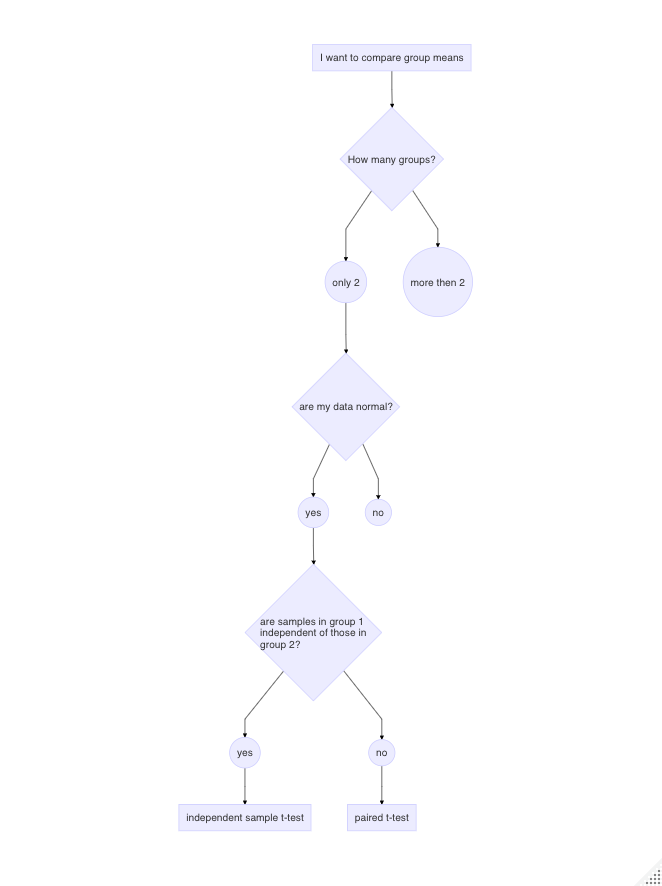
\includegraphics{/Users/jwalker/Documents/Github projects/Bookdown projects/applied-biostats/images/flowchart.png}
\caption{\label{fig:flowchart}A small flow chart demo of the flowchart strategy of statistical analysis. This chart covers a very small subset of potential paths that could be built from an introductory biostatistics textbook.}
\end{figure}

Compared to the flowchart stratgy, the advantages of the regression modeling strategy include

\begin{enumerate}
\def\labelenumi{\arabic{enumi}.}
\tightlist
\item
  A unified aproach in place of a collection of seemingly unrelated tests. The unifed approach is the \emph{regression model}.
\end{enumerate}

It has long been appreciated that classical regression, \emph{t}-tests, ANOVA, and other methods are all variations of the equation for a line \(Y = mX + b\) using slightly different notation

\begin{equation}
Y = \beta_0 + \beta_1 X + \varepsilon
\end{equation}

Chapter 1 explains the meaning of this notation but the point to make here is that because all regression models are variations of this equation, a modeling strategy of learning or doing statistics is more coherent than a flowchart strategy. Generalizations of this basic equation include general linear models, linear mixed models, generalized linear models, generalized additive models, causal graphical models, multivariate models, and machine learning. This book is not a comprehensive source for any of these methods but an introduction to the common foundations of all these methods.

\begin{enumerate}
\def\labelenumi{\arabic{enumi}.}
\setcounter{enumi}{1}
\tightlist
\item
  Estimates of effects and uncertainty are ultimately \emph{far} more useful than \emph{p}-values. For example, to build useful models on the effects of an increasingly acidified ocean on coral growth, we want to estimate the \emph{direction} and \emph{magnitude} of the effects at different levels of acidification and how these estimates change under different conditions. We can compare the magnitude to a prediction of the magnitude from a mechanistic model of growth. We can use a magnitude and uncertainty to make predictions about the future of coral reefs, under different scenarios of ocean acidification. We can use the estimated effects and uncertainty to model the consequences of the effects of acidification on coral growth on fish production or carbon cycling.
\end{enumerate}

By contrast, researchers learn little from a hypothesis test -- that is, comparing \emph{p} to 0.05. A \emph{p}-value is a measure of compatibility between the data and the null hypothesis and, consequently, a pretty good -- but imperfect -- tool to dampen the frequency that we are fooled by randomness. Importantly, a \emph{p}-value \textbf{is not a measure of the size of an effect}. At most, a small \emph{p}-value gives a researcher some confidence in the existence and direction of an effect. But if we are investigating the effects of acidified ocean water on coral growth, it would be absurd to conclude from a \emph{p}-value that pH does or does not affect growth. pH affects \emph{everything} about cell biology.

\emph{p}-values are neither necessary nor sufficient for good data analysis. Properly understood, a \emph{p}-value is a useful tool in the data analysis toolkit. As stated above, the proper use of \emph{p}-values dampens the frequency that we are fooled by randomness. Importantly, the estimation of effects and uncertainty and the computation of a \emph{p}-value are not alternatives. Indeed, the \emph{p}-value returned by many hypothesis tests are computed from the regression model used to estimate the effects. Throughout this text, statistical models are used to compute a \emph{p}-value \emph{in addition to} the estimates of effects and their uncertainty.

\textbf{NHST Blues} -- The ``discovery by p-value'' strategy, or Null-Hypothesis Significance Testing (NHST), has been criticized by statisticians for many, many decades. Nevertheless, introductory biostatistics textbooks written by both biologists and statisticians continue to organize textbooks around a collection of hypothesis tests, with much less emphasis on estimation and uncertainty. The NHST strategy of learning or doing statistics is easy in that it requires little understanding of the statistical model underneath the tests and its assumptions, limitations, and behavior. The NHST strategy in combination with point-and-click software enables ``mindless statistics''\footnote{Gegenrezer} and encourages the belief that statistics is a tool like a word processor is a tool, afterall, a rigorous analysis of one's data requires little more than getting p-values and creating bar plots. Indeed, many PhD programs in the biosciences require no statistics coursework and the only training available to students is from the other graduate students and postdocs in the lab. As a consequence, the biological sciences literature is filled with error bars that imply data with negative values and p-values that have little relationship to the probability of the data under the null. More importantly for science, the reported statistics are often not doing for the study what the researchers and journal editors think they are doing.

\hypertarget{math}{%
\section{Math}\label{math}}

\hypertarget{r-and-programming}{%
\section{R and programming}\label{r-and-programming}}

\hypertarget{a-completed-r-markdown-document}{%
\chapter*{A completed R Markdown document}\label{a-completed-r-markdown-document}}
\addcontentsline{toc}{chapter}{A completed R Markdown document}

Chapter 1 is a completed R Markdown document for a mini project -- think of it as a template for organizing your own R Markdown documents. This example is a re-analysis of the experiments in Figure 2 in the article \href{https://www.nature.com/articles/s41467-020-15483-7}{ASK1 inhibits browning of white adipose tissue in obesity} , including generation of the publication-ready plots. I chose this example, because of the diversity of analyses and plot types. My analyses and plots differ slightly from those of the researchers because I implemented better practices -- the stuff of this text.

A little background on the subject of the article: Mammalian brown adipose tissue (BAT) is composed of adipose (fat) cells that use the potential energy of the proton gradient across the inner mitochondrial membrane to generate heat instead of ATP. This is enabled by the facilitation of the protein \emph{uncoupling receptor 1} (UCP1). In response to health consequences of obesity, including metabolic syndrome, researchers are investigating various ways to increase BAT or stimulate BAT activity. One way to increase BAT is by signaling white adipose tissue (WAT) cells to ``brown'', that is, to transform into more BAT-like cells, by turning up expression of UCP1.

The researchers of ASK1 study investigated the effects of adipocyte-expressed apoptosis signal-regulating kinase 1 (ASK1) on the browning of white adipose tissue. For the experiments in Figure 2, the researchers created mice ``adipocyte-specific ASK1 knockout (KO) mice (ASK1Δadipo) on a C57BL/6 background using the Cre-lox system''. For the control, ``littermate mice with floxed ASK1 but lacking Cre expression under the adiponectin promotor were used (ASK1F/F)''. The KO and control mice were assigned to either Chow or a High Fat Diet (HFD). The experimental design is two-crossed factors, each with two levels, which I call a \(2 \times 2\) factorial design in this text.

\begin{itemize}
\item
  Some of the plots are coded directly in this document. Others use functions from the chapter ``Plotting functions''. But, to use these in an R Markdown document, these functions have to be saved in a ``R Script'' file. This script file then needs to be read at the start of the R Markdown document. I named the script file ``ggplotsci.R'' and placed it in a folder called ``R'' at the level of the project (directly within the project folder).
\item
  This example was written with the Bookdown style sheet (because its part of this book), which doesn't have one nice features of creating R Markdown documents for reports and manuscripts -- code folding. In an R Markdown document with code folding, a user can toggle between showing and hiding code. The html output with code folding is here.
\end{itemize}

\hypertarget{analysis-for-figure-2-of-ask1-inhibits-browning-of-white-adipose-tissue-in-obesity}{%
\chapter{Analysis for Figure 2 of ``ASK1 inhibits browning of white adipose tissue in obesity''}\label{analysis-for-figure-2-of-ask1-inhibits-browning-of-white-adipose-tissue-in-obesity}}

\begin{Shaded}
\begin{Highlighting}[]
\CommentTok{# wrangling packages}
\KeywordTok{library}\NormalTok{(here)}
\KeywordTok{library}\NormalTok{(janitor)}
\KeywordTok{library}\NormalTok{(readxl)}
\KeywordTok{library}\NormalTok{(data.table)}
\KeywordTok{library}\NormalTok{(stringr)}

\CommentTok{# analysis packages}
\KeywordTok{library}\NormalTok{(emmeans)}
\KeywordTok{library}\NormalTok{(car) }\CommentTok{# qqplot, spreadlevel}
\KeywordTok{library}\NormalTok{(DHARMa)}

\CommentTok{# graphing packages}
\KeywordTok{library}\NormalTok{(ggsci)}
\KeywordTok{library}\NormalTok{(ggpubr)}
\KeywordTok{library}\NormalTok{(ggforce)}
\KeywordTok{library}\NormalTok{(cowplot)}
\KeywordTok{library}\NormalTok{(lazyWeave) }\CommentTok{#pvalstring}

\NormalTok{here <-}\StringTok{ }\NormalTok{here}\OperatorTok{::}\KeywordTok{here}\NormalTok{()}
\NormalTok{data_path <-}\StringTok{ "data"}

\NormalTok{ggplotsci_path <-}\StringTok{ }\NormalTok{here}\OperatorTok{::}\KeywordTok{here}\NormalTok{(}\StringTok{"R"}\NormalTok{, }\StringTok{"ggplotsci.R"}\NormalTok{)}
\KeywordTok{source}\NormalTok{(ggplotsci_path)}
\end{Highlighting}
\end{Shaded}

Data source: \href{https://www.nature.com/articles/s41467-020-15483-7}{ASK1 inhibits browning of white adipose tissue in obesity}

This chunk assigns the path to the Excel data file for all panels of Figure 2. The data for each panel are in a single sheet in the Excel file named ``Source Date\_Figure 2''.

\begin{Shaded}
\begin{Highlighting}[]
\NormalTok{data_folder <-}\StringTok{ "ASK1 inhibits browning of white adipose tissue in obesity"}
\NormalTok{file_name <-}\StringTok{ "41467_2020_15483_MOESM4_ESM.xlsx"}
\NormalTok{file_path <-}\StringTok{ }\NormalTok{here}\OperatorTok{::}\KeywordTok{here}\NormalTok{(data_path, data_folder, file_name)}
  
\NormalTok{fig_}\DecValTok{2}\NormalTok{_sheet <-}\StringTok{ "Source Date_Figure 2"}
\end{Highlighting}
\end{Shaded}

\hypertarget{useful-functions}{%
\section{useful functions}\label{useful-functions}}

A function to import longitudinal data from Fig 2

\begin{Shaded}
\begin{Highlighting}[]
\CommentTok{# function to read in parts of 2b}
\NormalTok{import_fig_}\DecValTok{2}\NormalTok{_part <-}\StringTok{ }\ControlFlowTok{function}\NormalTok{(range_}\DecValTok{2}\NormalTok{)\{}
\NormalTok{  fig_}\DecValTok{2}\NormalTok{_part <-}\StringTok{ }\KeywordTok{read_excel}\NormalTok{(file_path,}
                          \DataTypeTok{sheet =}\NormalTok{ fig_}\DecValTok{2}\NormalTok{_sheet,}
                          \DataTypeTok{range =}\NormalTok{ range_}\DecValTok{2}\NormalTok{,}
                          \DataTypeTok{col_names =} \OtherTok{TRUE}\NormalTok{) }\OperatorTok
\StringTok{    }\KeywordTok{data.table}\NormalTok{()}
\NormalTok{  group <-}\StringTok{ }\KeywordTok{colnames}\NormalTok{(fig_}\DecValTok{2}\NormalTok{_part)[}\DecValTok{1}\NormalTok{]}
  \KeywordTok{setnames}\NormalTok{(fig_}\DecValTok{2}\NormalTok{_part, }\DataTypeTok{old =}\NormalTok{ group, }\DataTypeTok{new =} \StringTok{"treatment"}\NormalTok{)}
\NormalTok{  fig_}\DecValTok{2}\NormalTok{_part[, treatment }\OperatorTok{:}\ErrorTok{=}\StringTok{ }\KeywordTok{as.character}\NormalTok{(treatment)] }\CommentTok{# this was read as logical}
\NormalTok{  fig_}\DecValTok{2}\NormalTok{_part[, treatment }\OperatorTok{:}\ErrorTok{=}\StringTok{ }\NormalTok{group] }\CommentTok{# assign treatment group}
\NormalTok{  fig_}\DecValTok{2}\NormalTok{_part[, mouse_id }\OperatorTok{:}\ErrorTok{=}\StringTok{ }\KeywordTok{paste}\NormalTok{(group, .I)]}
  \KeywordTok{return}\NormalTok{(fig_}\DecValTok{2}\NormalTok{_part)}
\NormalTok{\}}
\end{Highlighting}
\end{Shaded}

\begin{Shaded}
\begin{Highlighting}[]
\CommentTok{# script to compute various area under the curves (AUC) using trapezoidal method}
\CommentTok{# le Floch's "incremental" auc substracts the baseline value from all points.}
\CommentTok{# This can create some elements with negative area if post-baseline values are less}
\CommentTok{# than baseline value.}
\CommentTok{# Some researchers "correct" this by setting any(y - ybar < 0 to zero. Don't do this.}

\NormalTok{auc <-}\StringTok{ }\ControlFlowTok{function}\NormalTok{(x, y, }\DataTypeTok{method=}\StringTok{"auc"}\NormalTok{, }\DataTypeTok{average =} \OtherTok{FALSE}\NormalTok{)\{}
  \CommentTok{# method = "auc", auc computed using trapezoidal calc}
  \CommentTok{# method = "iauc" is an incremental AUC of Le Floch}
  \CommentTok{# method = "pos_iauc" is a "positive" incremental AUC of Le Floch but not Wolever}
  \CommentTok{# method = "post_0_auc" is AUC of post-time0 values}
  \CommentTok{# if average then divide area by duration}
  \ControlFlowTok{if}\NormalTok{(method}\OperatorTok{==}\StringTok{"iauc"}\NormalTok{)\{y <-}\StringTok{ }\NormalTok{y }\OperatorTok{-}\StringTok{ }\NormalTok{y[}\DecValTok{1}\NormalTok{]\}}
  \ControlFlowTok{if}\NormalTok{(method}\OperatorTok{==}\StringTok{"pos_iauc"}\NormalTok{)\{y[y }\OperatorTok{<}\StringTok{ }\DecValTok{0}\NormalTok{] <-}\StringTok{ }\DecValTok{0}\NormalTok{\}}
  \ControlFlowTok{if}\NormalTok{(method}\OperatorTok{==}\StringTok{"post_0_auc"}\NormalTok{)\{}
\NormalTok{    x <-}\StringTok{ }\NormalTok{x[}\OperatorTok{-}\DecValTok{1}\NormalTok{]}
\NormalTok{    y <-}\StringTok{ }\NormalTok{y[}\OperatorTok{-}\DecValTok{1}\NormalTok{]}
\NormalTok{  \}}
\NormalTok{  n <-}\StringTok{ }\KeywordTok{length}\NormalTok{(x)}
\NormalTok{  area <-}\StringTok{ }\DecValTok{0}
  \ControlFlowTok{for}\NormalTok{(i }\ControlFlowTok{in} \DecValTok{2}\OperatorTok{:}\NormalTok{n)\{}
\NormalTok{    area <-}\StringTok{ }\NormalTok{area }\OperatorTok{+}\StringTok{ }\NormalTok{(x[i] }\OperatorTok{-}\StringTok{ }\NormalTok{x[i}\DecValTok{-1}\NormalTok{])}\OperatorTok{*}\NormalTok{(y[i}\DecValTok{-1}\NormalTok{] }\OperatorTok{+}\StringTok{ }\NormalTok{y[i])}
\NormalTok{  \}}
\NormalTok{  value <-}\StringTok{ }\NormalTok{area}\OperatorTok{/}\DecValTok{2}
  \ControlFlowTok{if}\NormalTok{(average }\OperatorTok{==}\StringTok{ }\OtherTok{TRUE}\NormalTok{)\{}
\NormalTok{    value <-}\StringTok{ }\NormalTok{value}\OperatorTok{/}\NormalTok{(x[}\KeywordTok{length}\NormalTok{(x)] }\OperatorTok{-}\StringTok{ }\NormalTok{x[}\DecValTok{1}\NormalTok{])}
\NormalTok{  \}}
  \KeywordTok{return}\NormalTok{(value)}
\NormalTok{\}}
\end{Highlighting}
\end{Shaded}

\begin{Shaded}
\begin{Highlighting}[]
\NormalTok{pal_nature_mod <-}\StringTok{ }\KeywordTok{c}\NormalTok{(}
  \StringTok{"#3DB7E9"}\NormalTok{, }\CommentTok{# summer sky}
  \StringTok{"#e69f00"}\NormalTok{, }\CommentTok{# gamboge, squash, buttercup}
  \StringTok{"#359B73"}\NormalTok{, }\CommentTok{# ocean green}
  \StringTok{"#2271B2"}\NormalTok{, }\CommentTok{# honolulu blue}
  \StringTok{"#f0e442"}\NormalTok{, }\CommentTok{# holiday, }
  \StringTok{"#F748A5"}\NormalTok{, }\CommentTok{# barbi pink}
  \StringTok{"#d55e00"} \CommentTok{# bamboo}
\NormalTok{)}
\end{Highlighting}
\end{Shaded}

\hypertarget{figure-2b-effect-of-ask1-ko-on-growth-body-weight}{%
\section{figure 2b -- effect of ASK1 KO on growth (body weight)}\label{figure-2b-effect-of-ask1-ko-on-growth-body-weight}}

\hypertarget{figure-2b-import}{%
\subsection{figure 2b -- import}\label{figure-2b-import}}

\begin{Shaded}
\begin{Highlighting}[]
\NormalTok{range_list <-}\StringTok{ }\KeywordTok{c}\NormalTok{(}\StringTok{"A21:N41"}\NormalTok{, }\StringTok{"A43:N56"}\NormalTok{, }\StringTok{"A58:N110"}\NormalTok{, }\StringTok{"A112:N170"}\NormalTok{)}
\NormalTok{fig_2b_wide <-}\StringTok{ }\KeywordTok{data.table}\NormalTok{(}\OtherTok{NULL}\NormalTok{)}
\ControlFlowTok{for}\NormalTok{(range_i }\ControlFlowTok{in}\NormalTok{ range_list)\{}
\NormalTok{  part <-}\StringTok{ }\KeywordTok{import_fig_2_part}\NormalTok{(range_i)}
\NormalTok{  fig_2b_wide <-}\StringTok{ }\KeywordTok{rbind}\NormalTok{(fig_2b_wide,}
\NormalTok{                       part)}
\NormalTok{\}}

\NormalTok{fig_2b <-}\StringTok{ }\KeywordTok{melt}\NormalTok{(fig_2b_wide,}
               \DataTypeTok{id.vars =} \KeywordTok{c}\NormalTok{(}\StringTok{"treatment"}\NormalTok{, }\StringTok{"mouse_id"}\NormalTok{),}
               \DataTypeTok{variable.name =} \StringTok{"week"}\NormalTok{,}
               \DataTypeTok{value.name =} \StringTok{"body_weight"}\NormalTok{)}
\NormalTok{fig_2b[, week }\OperatorTok{:}\ErrorTok{=}\StringTok{ }\KeywordTok{as.numeric}\NormalTok{(}\KeywordTok{as.character}\NormalTok{(week))]}
\NormalTok{fig_2b[, }\KeywordTok{c}\NormalTok{(}\StringTok{"ask1"}\NormalTok{, }\StringTok{"diet"}\NormalTok{) }\OperatorTok{:}\ErrorTok{=}\StringTok{ }\KeywordTok{tstrsplit}\NormalTok{(treatment, }\StringTok{" "}\NormalTok{, }\DataTypeTok{fixed=}\OtherTok{TRUE}\NormalTok{)]}
\NormalTok{fig_2b[, week_f }\OperatorTok{:}\ErrorTok{=}\StringTok{ }\KeywordTok{factor}\NormalTok{(week)]}
\end{Highlighting}
\end{Shaded}

\hypertarget{figure-2b-exploratory-plots}{%
\subsection{figure 2b -- exploratory plots}\label{figure-2b-exploratory-plots}}

\begin{Shaded}
\begin{Highlighting}[]
\KeywordTok{qplot}\NormalTok{(}\DataTypeTok{x =}\NormalTok{ week,}
      \DataTypeTok{y =}\NormalTok{ body_weight,}
      \DataTypeTok{data =}\NormalTok{ fig_2b,}
      \DataTypeTok{color =}\NormalTok{ treatment) }\OperatorTok{+}
\StringTok{  }\KeywordTok{facet_grid}\NormalTok{(ask1}\OperatorTok{~}\NormalTok{diet)}
\end{Highlighting}
\end{Shaded}

\begin{verbatim}
## Warning in grid.Call(C_textBounds, as.graphicsAnnot(x$label), x$x, x$y, :
## conversion failure on 'ASK1Δadipo' in 'mbcsToSbcs': dot substituted for
## <ce>
\end{verbatim}

\begin{verbatim}
## Warning in grid.Call(C_textBounds, as.graphicsAnnot(x$label), x$x, x$y, :
## conversion failure on 'ASK1Δadipo' in 'mbcsToSbcs': dot substituted for
## <94>
\end{verbatim}

\begin{verbatim}
## Warning in grid.Call(C_textBounds, as.graphicsAnnot(x$label), x$x, x$y, :
## conversion failure on 'ASK1Δadipo' in 'mbcsToSbcs': dot substituted for
## <ce>
\end{verbatim}

\begin{verbatim}
## Warning in grid.Call(C_textBounds, as.graphicsAnnot(x$label), x$x, x$y, :
## conversion failure on 'ASK1Δadipo' in 'mbcsToSbcs': dot substituted for
## <94>
\end{verbatim}

\begin{verbatim}
## Warning in grid.Call(C_textBounds, as.graphicsAnnot(x$label), x$x, x$y, :
## conversion failure on 'ASK1Δadipo chow' in 'mbcsToSbcs': dot substituted
## for <ce>
\end{verbatim}

\begin{verbatim}
## Warning in grid.Call(C_textBounds, as.graphicsAnnot(x$label), x$x, x$y, :
## conversion failure on 'ASK1Δadipo chow' in 'mbcsToSbcs': dot substituted
## for <94>
\end{verbatim}

\begin{verbatim}
## Warning in grid.Call(C_textBounds, as.graphicsAnnot(x$label), x$x, x$y, :
## conversion failure on 'ASK1Δadipo chow' in 'mbcsToSbcs': dot substituted
## for <ce>
\end{verbatim}

\begin{verbatim}
## Warning in grid.Call(C_textBounds, as.graphicsAnnot(x$label), x$x, x$y, :
## conversion failure on 'ASK1Δadipo chow' in 'mbcsToSbcs': dot substituted
## for <94>
\end{verbatim}

\begin{verbatim}
## Warning in grid.Call(C_textBounds, as.graphicsAnnot(x$label), x$x, x$y, :
## conversion failure on 'ASK1Δadipo chow' in 'mbcsToSbcs': dot substituted
## for <ce>
\end{verbatim}

\begin{verbatim}
## Warning in grid.Call(C_textBounds, as.graphicsAnnot(x$label), x$x, x$y, :
## conversion failure on 'ASK1Δadipo chow' in 'mbcsToSbcs': dot substituted
## for <94>
\end{verbatim}

\begin{verbatim}
## Warning in grid.Call(C_textBounds, as.graphicsAnnot(x$label), x$x, x$y, :
## conversion failure on 'ASK1Δadipo chow' in 'mbcsToSbcs': dot substituted
## for <ce>
\end{verbatim}

\begin{verbatim}
## Warning in grid.Call(C_textBounds, as.graphicsAnnot(x$label), x$x, x$y, :
## conversion failure on 'ASK1Δadipo chow' in 'mbcsToSbcs': dot substituted
## for <94>
\end{verbatim}

\begin{verbatim}
## Warning in grid.Call(C_textBounds, as.graphicsAnnot(x$label), x$x, x$y, :
## conversion failure on 'ASK1Δadipo chow' in 'mbcsToSbcs': dot substituted
## for <ce>
\end{verbatim}

\begin{verbatim}
## Warning in grid.Call(C_textBounds, as.graphicsAnnot(x$label), x$x, x$y, :
## conversion failure on 'ASK1Δadipo chow' in 'mbcsToSbcs': dot substituted
## for <94>
\end{verbatim}

\begin{verbatim}
## Warning in grid.Call(C_textBounds, as.graphicsAnnot(x$label), x$x, x$y, :
## conversion failure on 'ASK1Δadipo HFD' in 'mbcsToSbcs': dot substituted for
## <ce>
\end{verbatim}

\begin{verbatim}
## Warning in grid.Call(C_textBounds, as.graphicsAnnot(x$label), x$x, x$y, :
## conversion failure on 'ASK1Δadipo HFD' in 'mbcsToSbcs': dot substituted for
## <94>
\end{verbatim}

\begin{verbatim}
## Warning in grid.Call(C_textBounds, as.graphicsAnnot(x$label), x$x, x$y, :
## conversion failure on 'ASK1Δadipo HFD' in 'mbcsToSbcs': dot substituted for
## <ce>
\end{verbatim}

\begin{verbatim}
## Warning in grid.Call(C_textBounds, as.graphicsAnnot(x$label), x$x, x$y, :
## conversion failure on 'ASK1Δadipo HFD' in 'mbcsToSbcs': dot substituted for
## <94>
\end{verbatim}

\begin{verbatim}
## Warning in grid.Call(C_textBounds, as.graphicsAnnot(x$label), x$x, x$y, :
## conversion failure on 'ASK1Δadipo HFD' in 'mbcsToSbcs': dot substituted for
## <ce>
\end{verbatim}

\begin{verbatim}
## Warning in grid.Call(C_textBounds, as.graphicsAnnot(x$label), x$x, x$y, :
## conversion failure on 'ASK1Δadipo HFD' in 'mbcsToSbcs': dot substituted for
## <94>
\end{verbatim}

\begin{verbatim}
## Warning in grid.Call(C_textBounds, as.graphicsAnnot(x$label), x$x, x$y, :
## conversion failure on 'ASK1Δadipo HFD' in 'mbcsToSbcs': dot substituted for
## <ce>
\end{verbatim}

\begin{verbatim}
## Warning in grid.Call(C_textBounds, as.graphicsAnnot(x$label), x$x, x$y, :
## conversion failure on 'ASK1Δadipo HFD' in 'mbcsToSbcs': dot substituted for
## <94>
\end{verbatim}

\begin{verbatim}
## Warning in grid.Call(C_textBounds, as.graphicsAnnot(x$label), x$x, x$y, :
## conversion failure on 'ASK1Δadipo HFD' in 'mbcsToSbcs': dot substituted for
## <ce>
\end{verbatim}

\begin{verbatim}
## Warning in grid.Call(C_textBounds, as.graphicsAnnot(x$label), x$x, x$y, :
## conversion failure on 'ASK1Δadipo HFD' in 'mbcsToSbcs': dot substituted for
## <94>
\end{verbatim}

\begin{verbatim}
## Warning in grid.Call(C_textBounds, as.graphicsAnnot(x$label), x$x, x$y, :
## conversion failure on 'ASK1Δadipo chow' in 'mbcsToSbcs': dot substituted
## for <ce>
\end{verbatim}

\begin{verbatim}
## Warning in grid.Call(C_textBounds, as.graphicsAnnot(x$label), x$x, x$y, :
## conversion failure on 'ASK1Δadipo chow' in 'mbcsToSbcs': dot substituted
## for <94>
\end{verbatim}

\begin{verbatim}
## Warning in grid.Call(C_textBounds, as.graphicsAnnot(x$label), x$x, x$y, :
## conversion failure on 'ASK1Δadipo chow' in 'mbcsToSbcs': dot substituted
## for <ce>
\end{verbatim}

\begin{verbatim}
## Warning in grid.Call(C_textBounds, as.graphicsAnnot(x$label), x$x, x$y, :
## conversion failure on 'ASK1Δadipo chow' in 'mbcsToSbcs': dot substituted
## for <94>
\end{verbatim}

\begin{verbatim}
## Warning in grid.Call(C_textBounds, as.graphicsAnnot(x$label), x$x, x$y, :
## conversion failure on 'ASK1Δadipo chow' in 'mbcsToSbcs': dot substituted
## for <ce>
\end{verbatim}

\begin{verbatim}
## Warning in grid.Call(C_textBounds, as.graphicsAnnot(x$label), x$x, x$y, :
## conversion failure on 'ASK1Δadipo chow' in 'mbcsToSbcs': dot substituted
## for <94>
\end{verbatim}

\begin{verbatim}
## Warning in grid.Call(C_textBounds, as.graphicsAnnot(x$label), x$x, x$y, :
## conversion failure on 'ASK1Δadipo chow' in 'mbcsToSbcs': dot substituted
## for <ce>
\end{verbatim}

\begin{verbatim}
## Warning in grid.Call(C_textBounds, as.graphicsAnnot(x$label), x$x, x$y, :
## conversion failure on 'ASK1Δadipo chow' in 'mbcsToSbcs': dot substituted
## for <94>
\end{verbatim}

\begin{verbatim}
## Warning in grid.Call(C_textBounds, as.graphicsAnnot(x$label), x$x, x$y, :
## conversion failure on 'ASK1Δadipo chow' in 'mbcsToSbcs': dot substituted
## for <ce>
\end{verbatim}

\begin{verbatim}
## Warning in grid.Call(C_textBounds, as.graphicsAnnot(x$label), x$x, x$y, :
## conversion failure on 'ASK1Δadipo chow' in 'mbcsToSbcs': dot substituted
## for <94>
\end{verbatim}

\begin{verbatim}
## Warning in grid.Call(C_textBounds, as.graphicsAnnot(x$label), x$x, x$y, :
## conversion failure on 'ASK1Δadipo HFD' in 'mbcsToSbcs': dot substituted for
## <ce>
\end{verbatim}

\begin{verbatim}
## Warning in grid.Call(C_textBounds, as.graphicsAnnot(x$label), x$x, x$y, :
## conversion failure on 'ASK1Δadipo HFD' in 'mbcsToSbcs': dot substituted for
## <94>
\end{verbatim}

\begin{verbatim}
## Warning in grid.Call(C_textBounds, as.graphicsAnnot(x$label), x$x, x$y, :
## conversion failure on 'ASK1Δadipo HFD' in 'mbcsToSbcs': dot substituted for
## <ce>
\end{verbatim}

\begin{verbatim}
## Warning in grid.Call(C_textBounds, as.graphicsAnnot(x$label), x$x, x$y, :
## conversion failure on 'ASK1Δadipo HFD' in 'mbcsToSbcs': dot substituted for
## <94>
\end{verbatim}

\begin{verbatim}
## Warning in grid.Call(C_textBounds, as.graphicsAnnot(x$label), x$x, x$y, :
## conversion failure on 'ASK1Δadipo HFD' in 'mbcsToSbcs': dot substituted for
## <ce>
\end{verbatim}

\begin{verbatim}
## Warning in grid.Call(C_textBounds, as.graphicsAnnot(x$label), x$x, x$y, :
## conversion failure on 'ASK1Δadipo HFD' in 'mbcsToSbcs': dot substituted for
## <94>
\end{verbatim}

\begin{verbatim}
## Warning in grid.Call(C_textBounds, as.graphicsAnnot(x$label), x$x, x$y, :
## conversion failure on 'ASK1Δadipo HFD' in 'mbcsToSbcs': dot substituted for
## <ce>
\end{verbatim}

\begin{verbatim}
## Warning in grid.Call(C_textBounds, as.graphicsAnnot(x$label), x$x, x$y, :
## conversion failure on 'ASK1Δadipo HFD' in 'mbcsToSbcs': dot substituted for
## <94>
\end{verbatim}

\begin{verbatim}
## Warning in grid.Call(C_textBounds, as.graphicsAnnot(x$label), x$x, x$y, :
## conversion failure on 'ASK1Δadipo HFD' in 'mbcsToSbcs': dot substituted for
## <ce>
\end{verbatim}

\begin{verbatim}
## Warning in grid.Call(C_textBounds, as.graphicsAnnot(x$label), x$x, x$y, :
## conversion failure on 'ASK1Δadipo HFD' in 'mbcsToSbcs': dot substituted for
## <94>
\end{verbatim}

\begin{verbatim}
## Warning in grid.Call.graphics(C_text, as.graphicsAnnot(x$label), x$x,
## x$y, : conversion failure on 'ASK1Δadipo' in 'mbcsToSbcs': dot substituted
## for <ce>
\end{verbatim}

\begin{verbatim}
## Warning in grid.Call.graphics(C_text, as.graphicsAnnot(x$label), x$x,
## x$y, : conversion failure on 'ASK1Δadipo' in 'mbcsToSbcs': dot substituted
## for <94>
\end{verbatim}

\begin{verbatim}
## Warning in grid.Call(C_textBounds, as.graphicsAnnot(x$label), x$x, x$y, :
## conversion failure on 'ASK1Δadipo chow' in 'mbcsToSbcs': dot substituted
## for <ce>
\end{verbatim}

\begin{verbatim}
## Warning in grid.Call(C_textBounds, as.graphicsAnnot(x$label), x$x, x$y, :
## conversion failure on 'ASK1Δadipo chow' in 'mbcsToSbcs': dot substituted
## for <94>
\end{verbatim}

\begin{verbatim}
## Warning in grid.Call(C_textBounds, as.graphicsAnnot(x$label), x$x, x$y, :
## conversion failure on 'ASK1Δadipo chow' in 'mbcsToSbcs': dot substituted
## for <ce>
\end{verbatim}

\begin{verbatim}
## Warning in grid.Call(C_textBounds, as.graphicsAnnot(x$label), x$x, x$y, :
## conversion failure on 'ASK1Δadipo chow' in 'mbcsToSbcs': dot substituted
## for <94>
\end{verbatim}

\begin{verbatim}
## Warning in grid.Call(C_textBounds, as.graphicsAnnot(x$label), x$x, x$y, :
## conversion failure on 'ASK1Δadipo chow' in 'mbcsToSbcs': dot substituted
## for <ce>
\end{verbatim}

\begin{verbatim}
## Warning in grid.Call(C_textBounds, as.graphicsAnnot(x$label), x$x, x$y, :
## conversion failure on 'ASK1Δadipo chow' in 'mbcsToSbcs': dot substituted
## for <94>
\end{verbatim}

\begin{verbatim}
## Warning in grid.Call(C_textBounds, as.graphicsAnnot(x$label), x$x, x$y, :
## conversion failure on 'ASK1Δadipo chow' in 'mbcsToSbcs': dot substituted
## for <ce>
\end{verbatim}

\begin{verbatim}
## Warning in grid.Call(C_textBounds, as.graphicsAnnot(x$label), x$x, x$y, :
## conversion failure on 'ASK1Δadipo chow' in 'mbcsToSbcs': dot substituted
## for <94>
\end{verbatim}

\begin{verbatim}
## Warning in grid.Call(C_textBounds, as.graphicsAnnot(x$label), x$x, x$y, :
## conversion failure on 'ASK1Δadipo chow' in 'mbcsToSbcs': dot substituted
## for <ce>
\end{verbatim}

\begin{verbatim}
## Warning in grid.Call(C_textBounds, as.graphicsAnnot(x$label), x$x, x$y, :
## conversion failure on 'ASK1Δadipo chow' in 'mbcsToSbcs': dot substituted
## for <94>
\end{verbatim}

\begin{verbatim}
## Warning in grid.Call(C_textBounds, as.graphicsAnnot(x$label), x$x, x$y, :
## conversion failure on 'ASK1Δadipo chow' in 'mbcsToSbcs': dot substituted
## for <ce>
\end{verbatim}

\begin{verbatim}
## Warning in grid.Call(C_textBounds, as.graphicsAnnot(x$label), x$x, x$y, :
## conversion failure on 'ASK1Δadipo chow' in 'mbcsToSbcs': dot substituted
## for <94>
\end{verbatim}

\begin{verbatim}
## Warning in grid.Call(C_textBounds, as.graphicsAnnot(x$label), x$x, x$y, :
## conversion failure on 'ASK1Δadipo chow' in 'mbcsToSbcs': dot substituted
## for <ce>
\end{verbatim}

\begin{verbatim}
## Warning in grid.Call(C_textBounds, as.graphicsAnnot(x$label), x$x, x$y, :
## conversion failure on 'ASK1Δadipo chow' in 'mbcsToSbcs': dot substituted
## for <94>
\end{verbatim}

\begin{verbatim}
## Warning in grid.Call(C_textBounds, as.graphicsAnnot(x$label), x$x, x$y, :
## conversion failure on 'ASK1Δadipo chow' in 'mbcsToSbcs': dot substituted
## for <ce>
\end{verbatim}

\begin{verbatim}
## Warning in grid.Call(C_textBounds, as.graphicsAnnot(x$label), x$x, x$y, :
## conversion failure on 'ASK1Δadipo chow' in 'mbcsToSbcs': dot substituted
## for <94>
\end{verbatim}

\begin{verbatim}
## Warning in grid.Call(C_textBounds, as.graphicsAnnot(x$label), x$x, x$y, :
## conversion failure on 'ASK1Δadipo chow' in 'mbcsToSbcs': dot substituted
## for <ce>
\end{verbatim}

\begin{verbatim}
## Warning in grid.Call(C_textBounds, as.graphicsAnnot(x$label), x$x, x$y, :
## conversion failure on 'ASK1Δadipo chow' in 'mbcsToSbcs': dot substituted
## for <94>
\end{verbatim}

\begin{verbatim}
## Warning in grid.Call(C_textBounds, as.graphicsAnnot(x$label), x$x, x$y, :
## conversion failure on 'ASK1Δadipo chow' in 'mbcsToSbcs': dot substituted
## for <ce>
\end{verbatim}

\begin{verbatim}
## Warning in grid.Call(C_textBounds, as.graphicsAnnot(x$label), x$x, x$y, :
## conversion failure on 'ASK1Δadipo chow' in 'mbcsToSbcs': dot substituted
## for <94>
\end{verbatim}

\begin{verbatim}
## Warning in grid.Call(C_textBounds, as.graphicsAnnot(x$label), x$x, x$y, :
## conversion failure on 'ASK1Δadipo chow' in 'mbcsToSbcs': dot substituted
## for <ce>
\end{verbatim}

\begin{verbatim}
## Warning in grid.Call(C_textBounds, as.graphicsAnnot(x$label), x$x, x$y, :
## conversion failure on 'ASK1Δadipo chow' in 'mbcsToSbcs': dot substituted
## for <94>
\end{verbatim}

\begin{verbatim}
## Warning in grid.Call(C_textBounds, as.graphicsAnnot(x$label), x$x, x$y, :
## conversion failure on 'ASK1Δadipo chow' in 'mbcsToSbcs': dot substituted
## for <ce>
\end{verbatim}

\begin{verbatim}
## Warning in grid.Call(C_textBounds, as.graphicsAnnot(x$label), x$x, x$y, :
## conversion failure on 'ASK1Δadipo chow' in 'mbcsToSbcs': dot substituted
## for <94>
\end{verbatim}

\begin{verbatim}
## Warning in grid.Call(C_textBounds, as.graphicsAnnot(x$label), x$x, x$y, :
## conversion failure on 'ASK1Δadipo chow' in 'mbcsToSbcs': dot substituted
## for <ce>
\end{verbatim}

\begin{verbatim}
## Warning in grid.Call(C_textBounds, as.graphicsAnnot(x$label), x$x, x$y, :
## conversion failure on 'ASK1Δadipo chow' in 'mbcsToSbcs': dot substituted
## for <94>
\end{verbatim}

\begin{verbatim}
## Warning in grid.Call(C_textBounds, as.graphicsAnnot(x$label), x$x, x$y, :
## conversion failure on 'ASK1Δadipo chow' in 'mbcsToSbcs': dot substituted
## for <ce>
\end{verbatim}

\begin{verbatim}
## Warning in grid.Call(C_textBounds, as.graphicsAnnot(x$label), x$x, x$y, :
## conversion failure on 'ASK1Δadipo chow' in 'mbcsToSbcs': dot substituted
## for <94>
\end{verbatim}

\begin{verbatim}
## Warning in grid.Call.graphics(C_text, as.graphicsAnnot(x$label), x$x,
## x$y, : conversion failure on 'ASK1Δadipo chow' in 'mbcsToSbcs': dot
## substituted for <ce>
\end{verbatim}

\begin{verbatim}
## Warning in grid.Call.graphics(C_text, as.graphicsAnnot(x$label), x$x,
## x$y, : conversion failure on 'ASK1Δadipo chow' in 'mbcsToSbcs': dot
## substituted for <94>
\end{verbatim}

\begin{verbatim}
## Warning in grid.Call(C_textBounds, as.graphicsAnnot(x$label), x$x, x$y, :
## conversion failure on 'ASK1Δadipo HFD' in 'mbcsToSbcs': dot substituted for
## <ce>
\end{verbatim}

\begin{verbatim}
## Warning in grid.Call(C_textBounds, as.graphicsAnnot(x$label), x$x, x$y, :
## conversion failure on 'ASK1Δadipo HFD' in 'mbcsToSbcs': dot substituted for
## <94>
\end{verbatim}

\begin{verbatim}
## Warning in grid.Call(C_textBounds, as.graphicsAnnot(x$label), x$x, x$y, :
## conversion failure on 'ASK1Δadipo HFD' in 'mbcsToSbcs': dot substituted for
## <ce>
\end{verbatim}

\begin{verbatim}
## Warning in grid.Call(C_textBounds, as.graphicsAnnot(x$label), x$x, x$y, :
## conversion failure on 'ASK1Δadipo HFD' in 'mbcsToSbcs': dot substituted for
## <94>
\end{verbatim}

\begin{verbatim}
## Warning in grid.Call(C_textBounds, as.graphicsAnnot(x$label), x$x, x$y, :
## conversion failure on 'ASK1Δadipo HFD' in 'mbcsToSbcs': dot substituted for
## <ce>
\end{verbatim}

\begin{verbatim}
## Warning in grid.Call(C_textBounds, as.graphicsAnnot(x$label), x$x, x$y, :
## conversion failure on 'ASK1Δadipo HFD' in 'mbcsToSbcs': dot substituted for
## <94>
\end{verbatim}

\begin{verbatim}
## Warning in grid.Call(C_textBounds, as.graphicsAnnot(x$label), x$x, x$y, :
## conversion failure on 'ASK1Δadipo HFD' in 'mbcsToSbcs': dot substituted for
## <ce>
\end{verbatim}

\begin{verbatim}
## Warning in grid.Call(C_textBounds, as.graphicsAnnot(x$label), x$x, x$y, :
## conversion failure on 'ASK1Δadipo HFD' in 'mbcsToSbcs': dot substituted for
## <94>
\end{verbatim}

\begin{verbatim}
## Warning in grid.Call(C_textBounds, as.graphicsAnnot(x$label), x$x, x$y, :
## conversion failure on 'ASK1Δadipo HFD' in 'mbcsToSbcs': dot substituted for
## <ce>
\end{verbatim}

\begin{verbatim}
## Warning in grid.Call(C_textBounds, as.graphicsAnnot(x$label), x$x, x$y, :
## conversion failure on 'ASK1Δadipo HFD' in 'mbcsToSbcs': dot substituted for
## <94>
\end{verbatim}

\begin{verbatim}
## Warning in grid.Call(C_textBounds, as.graphicsAnnot(x$label), x$x, x$y, :
## conversion failure on 'ASK1Δadipo HFD' in 'mbcsToSbcs': dot substituted for
## <ce>
\end{verbatim}

\begin{verbatim}
## Warning in grid.Call(C_textBounds, as.graphicsAnnot(x$label), x$x, x$y, :
## conversion failure on 'ASK1Δadipo HFD' in 'mbcsToSbcs': dot substituted for
## <94>
\end{verbatim}

\begin{verbatim}
## Warning in grid.Call(C_textBounds, as.graphicsAnnot(x$label), x$x, x$y, :
## conversion failure on 'ASK1Δadipo HFD' in 'mbcsToSbcs': dot substituted for
## <ce>
\end{verbatim}

\begin{verbatim}
## Warning in grid.Call(C_textBounds, as.graphicsAnnot(x$label), x$x, x$y, :
## conversion failure on 'ASK1Δadipo HFD' in 'mbcsToSbcs': dot substituted for
## <94>
\end{verbatim}

\begin{verbatim}
## Warning in grid.Call(C_textBounds, as.graphicsAnnot(x$label), x$x, x$y, :
## conversion failure on 'ASK1Δadipo HFD' in 'mbcsToSbcs': dot substituted for
## <ce>
\end{verbatim}

\begin{verbatim}
## Warning in grid.Call(C_textBounds, as.graphicsAnnot(x$label), x$x, x$y, :
## conversion failure on 'ASK1Δadipo HFD' in 'mbcsToSbcs': dot substituted for
## <94>
\end{verbatim}

\begin{verbatim}
## Warning in grid.Call(C_textBounds, as.graphicsAnnot(x$label), x$x, x$y, :
## conversion failure on 'ASK1Δadipo HFD' in 'mbcsToSbcs': dot substituted for
## <ce>
\end{verbatim}

\begin{verbatim}
## Warning in grid.Call(C_textBounds, as.graphicsAnnot(x$label), x$x, x$y, :
## conversion failure on 'ASK1Δadipo HFD' in 'mbcsToSbcs': dot substituted for
## <94>
\end{verbatim}

\begin{verbatim}
## Warning in grid.Call(C_textBounds, as.graphicsAnnot(x$label), x$x, x$y, :
## conversion failure on 'ASK1Δadipo HFD' in 'mbcsToSbcs': dot substituted for
## <ce>
\end{verbatim}

\begin{verbatim}
## Warning in grid.Call(C_textBounds, as.graphicsAnnot(x$label), x$x, x$y, :
## conversion failure on 'ASK1Δadipo HFD' in 'mbcsToSbcs': dot substituted for
## <94>
\end{verbatim}

\begin{verbatim}
## Warning in grid.Call(C_textBounds, as.graphicsAnnot(x$label), x$x, x$y, :
## conversion failure on 'ASK1Δadipo HFD' in 'mbcsToSbcs': dot substituted for
## <ce>
\end{verbatim}

\begin{verbatim}
## Warning in grid.Call(C_textBounds, as.graphicsAnnot(x$label), x$x, x$y, :
## conversion failure on 'ASK1Δadipo HFD' in 'mbcsToSbcs': dot substituted for
## <94>
\end{verbatim}

\begin{verbatim}
## Warning in grid.Call(C_textBounds, as.graphicsAnnot(x$label), x$x, x$y, :
## conversion failure on 'ASK1Δadipo HFD' in 'mbcsToSbcs': dot substituted for
## <ce>
\end{verbatim}

\begin{verbatim}
## Warning in grid.Call(C_textBounds, as.graphicsAnnot(x$label), x$x, x$y, :
## conversion failure on 'ASK1Δadipo HFD' in 'mbcsToSbcs': dot substituted for
## <94>
\end{verbatim}

\begin{verbatim}
## Warning in grid.Call(C_textBounds, as.graphicsAnnot(x$label), x$x, x$y, :
## conversion failure on 'ASK1Δadipo HFD' in 'mbcsToSbcs': dot substituted for
## <ce>
\end{verbatim}

\begin{verbatim}
## Warning in grid.Call(C_textBounds, as.graphicsAnnot(x$label), x$x, x$y, :
## conversion failure on 'ASK1Δadipo HFD' in 'mbcsToSbcs': dot substituted for
## <94>
\end{verbatim}

\begin{verbatim}
## Warning in grid.Call(C_textBounds, as.graphicsAnnot(x$label), x$x, x$y, :
## conversion failure on 'ASK1Δadipo HFD' in 'mbcsToSbcs': dot substituted for
## <ce>
\end{verbatim}

\begin{verbatim}
## Warning in grid.Call(C_textBounds, as.graphicsAnnot(x$label), x$x, x$y, :
## conversion failure on 'ASK1Δadipo HFD' in 'mbcsToSbcs': dot substituted for
## <94>
\end{verbatim}

\begin{verbatim}
## Warning in grid.Call.graphics(C_text, as.graphicsAnnot(x$label), x$x,
## x$y, : conversion failure on 'ASK1Δadipo HFD' in 'mbcsToSbcs': dot
## substituted for <ce>
\end{verbatim}

\begin{verbatim}
## Warning in grid.Call.graphics(C_text, as.graphicsAnnot(x$label), x$x,
## x$y, : conversion failure on 'ASK1Δadipo HFD' in 'mbcsToSbcs': dot
## substituted for <94>
\end{verbatim}

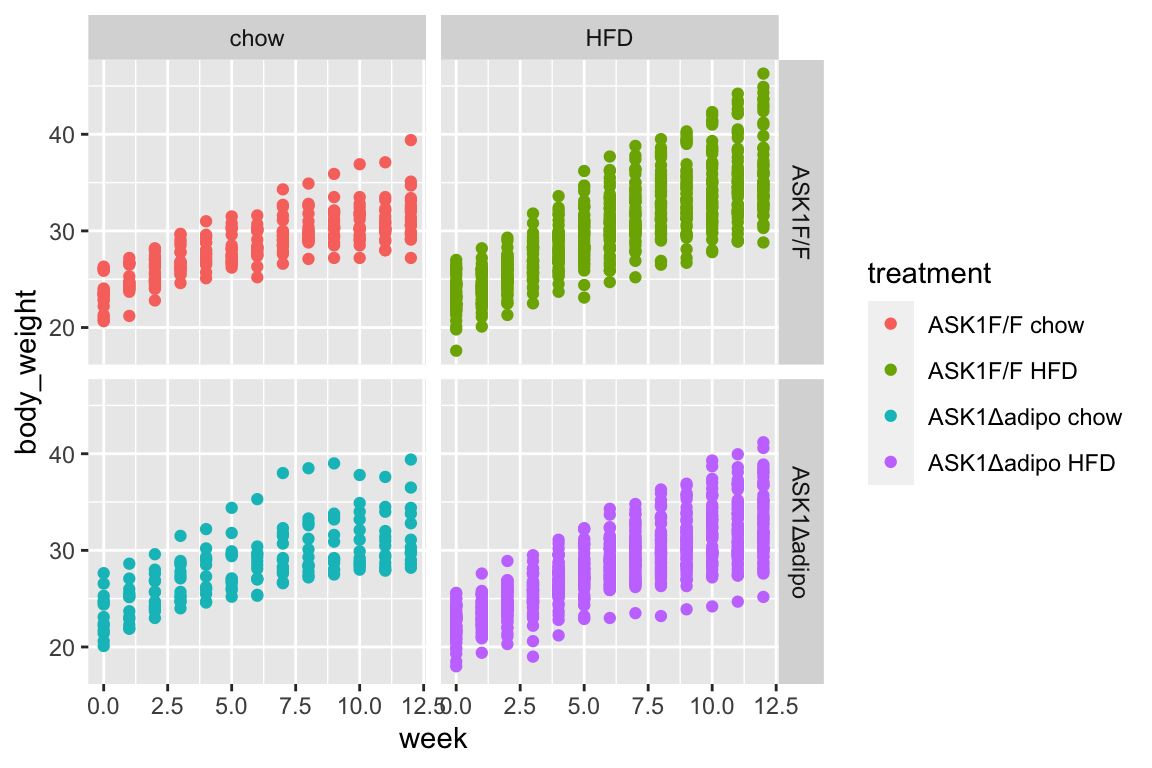
\includegraphics{Walker-elementary-statistical-modeling-draft_files/figure-latex/target-fig2b-initial-plot-1-1.pdf}

\begin{enumerate}
\def\labelenumi{\arabic{enumi}.}
\tightlist
\item
  no obvious outliers
\item
  reduced growth rate at bigger size
\end{enumerate}

\begin{Shaded}
\begin{Highlighting}[]
\KeywordTok{qplot}\NormalTok{(}\DataTypeTok{x =}\NormalTok{ week,}
      \DataTypeTok{y =}\NormalTok{ body_weight,}
      \DataTypeTok{data =}\NormalTok{ fig_2b,}
      \DataTypeTok{color =}\NormalTok{ treatment) }\OperatorTok{+}
\StringTok{  }\KeywordTok{geom_smooth}\NormalTok{()}
\end{Highlighting}
\end{Shaded}

\begin{verbatim}
## `geom_smooth()` using method = 'loess' and formula 'y ~ x'
\end{verbatim}

\begin{verbatim}
## Warning in grid.Call(C_textBounds, as.graphicsAnnot(x$label), x$x, x$y, :
## conversion failure on 'ASK1Δadipo chow' in 'mbcsToSbcs': dot substituted
## for <ce>
\end{verbatim}

\begin{verbatim}
## Warning in grid.Call(C_textBounds, as.graphicsAnnot(x$label), x$x, x$y, :
## conversion failure on 'ASK1Δadipo chow' in 'mbcsToSbcs': dot substituted
## for <94>
\end{verbatim}

\begin{verbatim}
## Warning in grid.Call(C_textBounds, as.graphicsAnnot(x$label), x$x, x$y, :
## conversion failure on 'ASK1Δadipo chow' in 'mbcsToSbcs': dot substituted
## for <ce>
\end{verbatim}

\begin{verbatim}
## Warning in grid.Call(C_textBounds, as.graphicsAnnot(x$label), x$x, x$y, :
## conversion failure on 'ASK1Δadipo chow' in 'mbcsToSbcs': dot substituted
## for <94>
\end{verbatim}

\begin{verbatim}
## Warning in grid.Call(C_textBounds, as.graphicsAnnot(x$label), x$x, x$y, :
## conversion failure on 'ASK1Δadipo chow' in 'mbcsToSbcs': dot substituted
## for <ce>
\end{verbatim}

\begin{verbatim}
## Warning in grid.Call(C_textBounds, as.graphicsAnnot(x$label), x$x, x$y, :
## conversion failure on 'ASK1Δadipo chow' in 'mbcsToSbcs': dot substituted
## for <94>
\end{verbatim}

\begin{verbatim}
## Warning in grid.Call(C_textBounds, as.graphicsAnnot(x$label), x$x, x$y, :
## conversion failure on 'ASK1Δadipo chow' in 'mbcsToSbcs': dot substituted
## for <ce>
\end{verbatim}

\begin{verbatim}
## Warning in grid.Call(C_textBounds, as.graphicsAnnot(x$label), x$x, x$y, :
## conversion failure on 'ASK1Δadipo chow' in 'mbcsToSbcs': dot substituted
## for <94>
\end{verbatim}

\begin{verbatim}
## Warning in grid.Call(C_textBounds, as.graphicsAnnot(x$label), x$x, x$y, :
## conversion failure on 'ASK1Δadipo chow' in 'mbcsToSbcs': dot substituted
## for <ce>
\end{verbatim}

\begin{verbatim}
## Warning in grid.Call(C_textBounds, as.graphicsAnnot(x$label), x$x, x$y, :
## conversion failure on 'ASK1Δadipo chow' in 'mbcsToSbcs': dot substituted
## for <94>
\end{verbatim}

\begin{verbatim}
## Warning in grid.Call(C_textBounds, as.graphicsAnnot(x$label), x$x, x$y, :
## conversion failure on 'ASK1Δadipo HFD' in 'mbcsToSbcs': dot substituted for
## <ce>
\end{verbatim}

\begin{verbatim}
## Warning in grid.Call(C_textBounds, as.graphicsAnnot(x$label), x$x, x$y, :
## conversion failure on 'ASK1Δadipo HFD' in 'mbcsToSbcs': dot substituted for
## <94>
\end{verbatim}

\begin{verbatim}
## Warning in grid.Call(C_textBounds, as.graphicsAnnot(x$label), x$x, x$y, :
## conversion failure on 'ASK1Δadipo HFD' in 'mbcsToSbcs': dot substituted for
## <ce>
\end{verbatim}

\begin{verbatim}
## Warning in grid.Call(C_textBounds, as.graphicsAnnot(x$label), x$x, x$y, :
## conversion failure on 'ASK1Δadipo HFD' in 'mbcsToSbcs': dot substituted for
## <94>
\end{verbatim}

\begin{verbatim}
## Warning in grid.Call(C_textBounds, as.graphicsAnnot(x$label), x$x, x$y, :
## conversion failure on 'ASK1Δadipo HFD' in 'mbcsToSbcs': dot substituted for
## <ce>
\end{verbatim}

\begin{verbatim}
## Warning in grid.Call(C_textBounds, as.graphicsAnnot(x$label), x$x, x$y, :
## conversion failure on 'ASK1Δadipo HFD' in 'mbcsToSbcs': dot substituted for
## <94>
\end{verbatim}

\begin{verbatim}
## Warning in grid.Call(C_textBounds, as.graphicsAnnot(x$label), x$x, x$y, :
## conversion failure on 'ASK1Δadipo HFD' in 'mbcsToSbcs': dot substituted for
## <ce>
\end{verbatim}

\begin{verbatim}
## Warning in grid.Call(C_textBounds, as.graphicsAnnot(x$label), x$x, x$y, :
## conversion failure on 'ASK1Δadipo HFD' in 'mbcsToSbcs': dot substituted for
## <94>
\end{verbatim}

\begin{verbatim}
## Warning in grid.Call(C_textBounds, as.graphicsAnnot(x$label), x$x, x$y, :
## conversion failure on 'ASK1Δadipo HFD' in 'mbcsToSbcs': dot substituted for
## <ce>
\end{verbatim}

\begin{verbatim}
## Warning in grid.Call(C_textBounds, as.graphicsAnnot(x$label), x$x, x$y, :
## conversion failure on 'ASK1Δadipo HFD' in 'mbcsToSbcs': dot substituted for
## <94>
\end{verbatim}

\begin{verbatim}
## Warning in grid.Call(C_textBounds, as.graphicsAnnot(x$label), x$x, x$y, :
## conversion failure on 'ASK1Δadipo chow' in 'mbcsToSbcs': dot substituted
## for <ce>
\end{verbatim}

\begin{verbatim}
## Warning in grid.Call(C_textBounds, as.graphicsAnnot(x$label), x$x, x$y, :
## conversion failure on 'ASK1Δadipo chow' in 'mbcsToSbcs': dot substituted
## for <94>
\end{verbatim}

\begin{verbatim}
## Warning in grid.Call(C_textBounds, as.graphicsAnnot(x$label), x$x, x$y, :
## conversion failure on 'ASK1Δadipo chow' in 'mbcsToSbcs': dot substituted
## for <ce>
\end{verbatim}

\begin{verbatim}
## Warning in grid.Call(C_textBounds, as.graphicsAnnot(x$label), x$x, x$y, :
## conversion failure on 'ASK1Δadipo chow' in 'mbcsToSbcs': dot substituted
## for <94>
\end{verbatim}

\begin{verbatim}
## Warning in grid.Call(C_textBounds, as.graphicsAnnot(x$label), x$x, x$y, :
## conversion failure on 'ASK1Δadipo chow' in 'mbcsToSbcs': dot substituted
## for <ce>
\end{verbatim}

\begin{verbatim}
## Warning in grid.Call(C_textBounds, as.graphicsAnnot(x$label), x$x, x$y, :
## conversion failure on 'ASK1Δadipo chow' in 'mbcsToSbcs': dot substituted
## for <94>
\end{verbatim}

\begin{verbatim}
## Warning in grid.Call(C_textBounds, as.graphicsAnnot(x$label), x$x, x$y, :
## conversion failure on 'ASK1Δadipo chow' in 'mbcsToSbcs': dot substituted
## for <ce>
\end{verbatim}

\begin{verbatim}
## Warning in grid.Call(C_textBounds, as.graphicsAnnot(x$label), x$x, x$y, :
## conversion failure on 'ASK1Δadipo chow' in 'mbcsToSbcs': dot substituted
## for <94>
\end{verbatim}

\begin{verbatim}
## Warning in grid.Call(C_textBounds, as.graphicsAnnot(x$label), x$x, x$y, :
## conversion failure on 'ASK1Δadipo chow' in 'mbcsToSbcs': dot substituted
## for <ce>
\end{verbatim}

\begin{verbatim}
## Warning in grid.Call(C_textBounds, as.graphicsAnnot(x$label), x$x, x$y, :
## conversion failure on 'ASK1Δadipo chow' in 'mbcsToSbcs': dot substituted
## for <94>
\end{verbatim}

\begin{verbatim}
## Warning in grid.Call(C_textBounds, as.graphicsAnnot(x$label), x$x, x$y, :
## conversion failure on 'ASK1Δadipo HFD' in 'mbcsToSbcs': dot substituted for
## <ce>
\end{verbatim}

\begin{verbatim}
## Warning in grid.Call(C_textBounds, as.graphicsAnnot(x$label), x$x, x$y, :
## conversion failure on 'ASK1Δadipo HFD' in 'mbcsToSbcs': dot substituted for
## <94>
\end{verbatim}

\begin{verbatim}
## Warning in grid.Call(C_textBounds, as.graphicsAnnot(x$label), x$x, x$y, :
## conversion failure on 'ASK1Δadipo HFD' in 'mbcsToSbcs': dot substituted for
## <ce>
\end{verbatim}

\begin{verbatim}
## Warning in grid.Call(C_textBounds, as.graphicsAnnot(x$label), x$x, x$y, :
## conversion failure on 'ASK1Δadipo HFD' in 'mbcsToSbcs': dot substituted for
## <94>
\end{verbatim}

\begin{verbatim}
## Warning in grid.Call(C_textBounds, as.graphicsAnnot(x$label), x$x, x$y, :
## conversion failure on 'ASK1Δadipo HFD' in 'mbcsToSbcs': dot substituted for
## <ce>
\end{verbatim}

\begin{verbatim}
## Warning in grid.Call(C_textBounds, as.graphicsAnnot(x$label), x$x, x$y, :
## conversion failure on 'ASK1Δadipo HFD' in 'mbcsToSbcs': dot substituted for
## <94>
\end{verbatim}

\begin{verbatim}
## Warning in grid.Call(C_textBounds, as.graphicsAnnot(x$label), x$x, x$y, :
## conversion failure on 'ASK1Δadipo HFD' in 'mbcsToSbcs': dot substituted for
## <ce>
\end{verbatim}

\begin{verbatim}
## Warning in grid.Call(C_textBounds, as.graphicsAnnot(x$label), x$x, x$y, :
## conversion failure on 'ASK1Δadipo HFD' in 'mbcsToSbcs': dot substituted for
## <94>
\end{verbatim}

\begin{verbatim}
## Warning in grid.Call(C_textBounds, as.graphicsAnnot(x$label), x$x, x$y, :
## conversion failure on 'ASK1Δadipo HFD' in 'mbcsToSbcs': dot substituted for
## <ce>
\end{verbatim}

\begin{verbatim}
## Warning in grid.Call(C_textBounds, as.graphicsAnnot(x$label), x$x, x$y, :
## conversion failure on 'ASK1Δadipo HFD' in 'mbcsToSbcs': dot substituted for
## <94>
\end{verbatim}

\begin{verbatim}
## Warning in grid.Call(C_textBounds, as.graphicsAnnot(x$label), x$x, x$y, :
## conversion failure on 'ASK1Δadipo chow' in 'mbcsToSbcs': dot substituted
## for <ce>
\end{verbatim}

\begin{verbatim}
## Warning in grid.Call(C_textBounds, as.graphicsAnnot(x$label), x$x, x$y, :
## conversion failure on 'ASK1Δadipo chow' in 'mbcsToSbcs': dot substituted
## for <94>
\end{verbatim}

\begin{verbatim}
## Warning in grid.Call(C_textBounds, as.graphicsAnnot(x$label), x$x, x$y, :
## conversion failure on 'ASK1Δadipo chow' in 'mbcsToSbcs': dot substituted
## for <ce>
\end{verbatim}

\begin{verbatim}
## Warning in grid.Call(C_textBounds, as.graphicsAnnot(x$label), x$x, x$y, :
## conversion failure on 'ASK1Δadipo chow' in 'mbcsToSbcs': dot substituted
## for <94>
\end{verbatim}

\begin{verbatim}
## Warning in grid.Call(C_textBounds, as.graphicsAnnot(x$label), x$x, x$y, :
## conversion failure on 'ASK1Δadipo chow' in 'mbcsToSbcs': dot substituted
## for <ce>
\end{verbatim}

\begin{verbatim}
## Warning in grid.Call(C_textBounds, as.graphicsAnnot(x$label), x$x, x$y, :
## conversion failure on 'ASK1Δadipo chow' in 'mbcsToSbcs': dot substituted
## for <94>
\end{verbatim}

\begin{verbatim}
## Warning in grid.Call(C_textBounds, as.graphicsAnnot(x$label), x$x, x$y, :
## conversion failure on 'ASK1Δadipo chow' in 'mbcsToSbcs': dot substituted
## for <ce>
\end{verbatim}

\begin{verbatim}
## Warning in grid.Call(C_textBounds, as.graphicsAnnot(x$label), x$x, x$y, :
## conversion failure on 'ASK1Δadipo chow' in 'mbcsToSbcs': dot substituted
## for <94>
\end{verbatim}

\begin{verbatim}
## Warning in grid.Call(C_textBounds, as.graphicsAnnot(x$label), x$x, x$y, :
## conversion failure on 'ASK1Δadipo chow' in 'mbcsToSbcs': dot substituted
## for <ce>
\end{verbatim}

\begin{verbatim}
## Warning in grid.Call(C_textBounds, as.graphicsAnnot(x$label), x$x, x$y, :
## conversion failure on 'ASK1Δadipo chow' in 'mbcsToSbcs': dot substituted
## for <94>
\end{verbatim}

\begin{verbatim}
## Warning in grid.Call(C_textBounds, as.graphicsAnnot(x$label), x$x, x$y, :
## conversion failure on 'ASK1Δadipo chow' in 'mbcsToSbcs': dot substituted
## for <ce>
\end{verbatim}

\begin{verbatim}
## Warning in grid.Call(C_textBounds, as.graphicsAnnot(x$label), x$x, x$y, :
## conversion failure on 'ASK1Δadipo chow' in 'mbcsToSbcs': dot substituted
## for <94>
\end{verbatim}

\begin{verbatim}
## Warning in grid.Call(C_textBounds, as.graphicsAnnot(x$label), x$x, x$y, :
## conversion failure on 'ASK1Δadipo chow' in 'mbcsToSbcs': dot substituted
## for <ce>
\end{verbatim}

\begin{verbatim}
## Warning in grid.Call(C_textBounds, as.graphicsAnnot(x$label), x$x, x$y, :
## conversion failure on 'ASK1Δadipo chow' in 'mbcsToSbcs': dot substituted
## for <94>
\end{verbatim}

\begin{verbatim}
## Warning in grid.Call(C_textBounds, as.graphicsAnnot(x$label), x$x, x$y, :
## conversion failure on 'ASK1Δadipo chow' in 'mbcsToSbcs': dot substituted
## for <ce>
\end{verbatim}

\begin{verbatim}
## Warning in grid.Call(C_textBounds, as.graphicsAnnot(x$label), x$x, x$y, :
## conversion failure on 'ASK1Δadipo chow' in 'mbcsToSbcs': dot substituted
## for <94>
\end{verbatim}

\begin{verbatim}
## Warning in grid.Call(C_textBounds, as.graphicsAnnot(x$label), x$x, x$y, :
## conversion failure on 'ASK1Δadipo chow' in 'mbcsToSbcs': dot substituted
## for <ce>
\end{verbatim}

\begin{verbatim}
## Warning in grid.Call(C_textBounds, as.graphicsAnnot(x$label), x$x, x$y, :
## conversion failure on 'ASK1Δadipo chow' in 'mbcsToSbcs': dot substituted
## for <94>
\end{verbatim}

\begin{verbatim}
## Warning in grid.Call(C_textBounds, as.graphicsAnnot(x$label), x$x, x$y, :
## conversion failure on 'ASK1Δadipo chow' in 'mbcsToSbcs': dot substituted
## for <ce>
\end{verbatim}

\begin{verbatim}
## Warning in grid.Call(C_textBounds, as.graphicsAnnot(x$label), x$x, x$y, :
## conversion failure on 'ASK1Δadipo chow' in 'mbcsToSbcs': dot substituted
## for <94>
\end{verbatim}

\begin{verbatim}
## Warning in grid.Call(C_textBounds, as.graphicsAnnot(x$label), x$x, x$y, :
## conversion failure on 'ASK1Δadipo chow' in 'mbcsToSbcs': dot substituted
## for <ce>
\end{verbatim}

\begin{verbatim}
## Warning in grid.Call(C_textBounds, as.graphicsAnnot(x$label), x$x, x$y, :
## conversion failure on 'ASK1Δadipo chow' in 'mbcsToSbcs': dot substituted
## for <94>
\end{verbatim}

\begin{verbatim}
## Warning in grid.Call(C_textBounds, as.graphicsAnnot(x$label), x$x, x$y, :
## conversion failure on 'ASK1Δadipo chow' in 'mbcsToSbcs': dot substituted
## for <ce>
\end{verbatim}

\begin{verbatim}
## Warning in grid.Call(C_textBounds, as.graphicsAnnot(x$label), x$x, x$y, :
## conversion failure on 'ASK1Δadipo chow' in 'mbcsToSbcs': dot substituted
## for <94>
\end{verbatim}

\begin{verbatim}
## Warning in grid.Call(C_textBounds, as.graphicsAnnot(x$label), x$x, x$y, :
## conversion failure on 'ASK1Δadipo chow' in 'mbcsToSbcs': dot substituted
## for <ce>
\end{verbatim}

\begin{verbatim}
## Warning in grid.Call(C_textBounds, as.graphicsAnnot(x$label), x$x, x$y, :
## conversion failure on 'ASK1Δadipo chow' in 'mbcsToSbcs': dot substituted
## for <94>
\end{verbatim}

\begin{verbatim}
## Warning in grid.Call(C_textBounds, as.graphicsAnnot(x$label), x$x, x$y, :
## conversion failure on 'ASK1Δadipo chow' in 'mbcsToSbcs': dot substituted
## for <ce>
\end{verbatim}

\begin{verbatim}
## Warning in grid.Call(C_textBounds, as.graphicsAnnot(x$label), x$x, x$y, :
## conversion failure on 'ASK1Δadipo chow' in 'mbcsToSbcs': dot substituted
## for <94>
\end{verbatim}

\begin{verbatim}
## Warning in grid.Call.graphics(C_text, as.graphicsAnnot(x$label), x$x,
## x$y, : conversion failure on 'ASK1Δadipo chow' in 'mbcsToSbcs': dot
## substituted for <ce>
\end{verbatim}

\begin{verbatim}
## Warning in grid.Call.graphics(C_text, as.graphicsAnnot(x$label), x$x,
## x$y, : conversion failure on 'ASK1Δadipo chow' in 'mbcsToSbcs': dot
## substituted for <94>
\end{verbatim}

\begin{verbatim}
## Warning in grid.Call(C_textBounds, as.graphicsAnnot(x$label), x$x, x$y, :
## conversion failure on 'ASK1Δadipo HFD' in 'mbcsToSbcs': dot substituted for
## <ce>
\end{verbatim}

\begin{verbatim}
## Warning in grid.Call(C_textBounds, as.graphicsAnnot(x$label), x$x, x$y, :
## conversion failure on 'ASK1Δadipo HFD' in 'mbcsToSbcs': dot substituted for
## <94>
\end{verbatim}

\begin{verbatim}
## Warning in grid.Call(C_textBounds, as.graphicsAnnot(x$label), x$x, x$y, :
## conversion failure on 'ASK1Δadipo HFD' in 'mbcsToSbcs': dot substituted for
## <ce>
\end{verbatim}

\begin{verbatim}
## Warning in grid.Call(C_textBounds, as.graphicsAnnot(x$label), x$x, x$y, :
## conversion failure on 'ASK1Δadipo HFD' in 'mbcsToSbcs': dot substituted for
## <94>
\end{verbatim}

\begin{verbatim}
## Warning in grid.Call(C_textBounds, as.graphicsAnnot(x$label), x$x, x$y, :
## conversion failure on 'ASK1Δadipo HFD' in 'mbcsToSbcs': dot substituted for
## <ce>
\end{verbatim}

\begin{verbatim}
## Warning in grid.Call(C_textBounds, as.graphicsAnnot(x$label), x$x, x$y, :
## conversion failure on 'ASK1Δadipo HFD' in 'mbcsToSbcs': dot substituted for
## <94>
\end{verbatim}

\begin{verbatim}
## Warning in grid.Call(C_textBounds, as.graphicsAnnot(x$label), x$x, x$y, :
## conversion failure on 'ASK1Δadipo HFD' in 'mbcsToSbcs': dot substituted for
## <ce>
\end{verbatim}

\begin{verbatim}
## Warning in grid.Call(C_textBounds, as.graphicsAnnot(x$label), x$x, x$y, :
## conversion failure on 'ASK1Δadipo HFD' in 'mbcsToSbcs': dot substituted for
## <94>
\end{verbatim}

\begin{verbatim}
## Warning in grid.Call(C_textBounds, as.graphicsAnnot(x$label), x$x, x$y, :
## conversion failure on 'ASK1Δadipo HFD' in 'mbcsToSbcs': dot substituted for
## <ce>
\end{verbatim}

\begin{verbatim}
## Warning in grid.Call(C_textBounds, as.graphicsAnnot(x$label), x$x, x$y, :
## conversion failure on 'ASK1Δadipo HFD' in 'mbcsToSbcs': dot substituted for
## <94>
\end{verbatim}

\begin{verbatim}
## Warning in grid.Call(C_textBounds, as.graphicsAnnot(x$label), x$x, x$y, :
## conversion failure on 'ASK1Δadipo HFD' in 'mbcsToSbcs': dot substituted for
## <ce>
\end{verbatim}

\begin{verbatim}
## Warning in grid.Call(C_textBounds, as.graphicsAnnot(x$label), x$x, x$y, :
## conversion failure on 'ASK1Δadipo HFD' in 'mbcsToSbcs': dot substituted for
## <94>
\end{verbatim}

\begin{verbatim}
## Warning in grid.Call(C_textBounds, as.graphicsAnnot(x$label), x$x, x$y, :
## conversion failure on 'ASK1Δadipo HFD' in 'mbcsToSbcs': dot substituted for
## <ce>
\end{verbatim}

\begin{verbatim}
## Warning in grid.Call(C_textBounds, as.graphicsAnnot(x$label), x$x, x$y, :
## conversion failure on 'ASK1Δadipo HFD' in 'mbcsToSbcs': dot substituted for
## <94>
\end{verbatim}

\begin{verbatim}
## Warning in grid.Call(C_textBounds, as.graphicsAnnot(x$label), x$x, x$y, :
## conversion failure on 'ASK1Δadipo HFD' in 'mbcsToSbcs': dot substituted for
## <ce>
\end{verbatim}

\begin{verbatim}
## Warning in grid.Call(C_textBounds, as.graphicsAnnot(x$label), x$x, x$y, :
## conversion failure on 'ASK1Δadipo HFD' in 'mbcsToSbcs': dot substituted for
## <94>
\end{verbatim}

\begin{verbatim}
## Warning in grid.Call(C_textBounds, as.graphicsAnnot(x$label), x$x, x$y, :
## conversion failure on 'ASK1Δadipo HFD' in 'mbcsToSbcs': dot substituted for
## <ce>
\end{verbatim}

\begin{verbatim}
## Warning in grid.Call(C_textBounds, as.graphicsAnnot(x$label), x$x, x$y, :
## conversion failure on 'ASK1Δadipo HFD' in 'mbcsToSbcs': dot substituted for
## <94>
\end{verbatim}

\begin{verbatim}
## Warning in grid.Call(C_textBounds, as.graphicsAnnot(x$label), x$x, x$y, :
## conversion failure on 'ASK1Δadipo HFD' in 'mbcsToSbcs': dot substituted for
## <ce>
\end{verbatim}

\begin{verbatim}
## Warning in grid.Call(C_textBounds, as.graphicsAnnot(x$label), x$x, x$y, :
## conversion failure on 'ASK1Δadipo HFD' in 'mbcsToSbcs': dot substituted for
## <94>
\end{verbatim}

\begin{verbatim}
## Warning in grid.Call(C_textBounds, as.graphicsAnnot(x$label), x$x, x$y, :
## conversion failure on 'ASK1Δadipo HFD' in 'mbcsToSbcs': dot substituted for
## <ce>
\end{verbatim}

\begin{verbatim}
## Warning in grid.Call(C_textBounds, as.graphicsAnnot(x$label), x$x, x$y, :
## conversion failure on 'ASK1Δadipo HFD' in 'mbcsToSbcs': dot substituted for
## <94>
\end{verbatim}

\begin{verbatim}
## Warning in grid.Call(C_textBounds, as.graphicsAnnot(x$label), x$x, x$y, :
## conversion failure on 'ASK1Δadipo HFD' in 'mbcsToSbcs': dot substituted for
## <ce>
\end{verbatim}

\begin{verbatim}
## Warning in grid.Call(C_textBounds, as.graphicsAnnot(x$label), x$x, x$y, :
## conversion failure on 'ASK1Δadipo HFD' in 'mbcsToSbcs': dot substituted for
## <94>
\end{verbatim}

\begin{verbatim}
## Warning in grid.Call(C_textBounds, as.graphicsAnnot(x$label), x$x, x$y, :
## conversion failure on 'ASK1Δadipo HFD' in 'mbcsToSbcs': dot substituted for
## <ce>
\end{verbatim}

\begin{verbatim}
## Warning in grid.Call(C_textBounds, as.graphicsAnnot(x$label), x$x, x$y, :
## conversion failure on 'ASK1Δadipo HFD' in 'mbcsToSbcs': dot substituted for
## <94>
\end{verbatim}

\begin{verbatim}
## Warning in grid.Call(C_textBounds, as.graphicsAnnot(x$label), x$x, x$y, :
## conversion failure on 'ASK1Δadipo HFD' in 'mbcsToSbcs': dot substituted for
## <ce>
\end{verbatim}

\begin{verbatim}
## Warning in grid.Call(C_textBounds, as.graphicsAnnot(x$label), x$x, x$y, :
## conversion failure on 'ASK1Δadipo HFD' in 'mbcsToSbcs': dot substituted for
## <94>
\end{verbatim}

\begin{verbatim}
## Warning in grid.Call.graphics(C_text, as.graphicsAnnot(x$label), x$x,
## x$y, : conversion failure on 'ASK1Δadipo HFD' in 'mbcsToSbcs': dot
## substituted for <ce>
\end{verbatim}

\begin{verbatim}
## Warning in grid.Call.graphics(C_text, as.graphicsAnnot(x$label), x$x,
## x$y, : conversion failure on 'ASK1Δadipo HFD' in 'mbcsToSbcs': dot
## substituted for <94>
\end{verbatim}

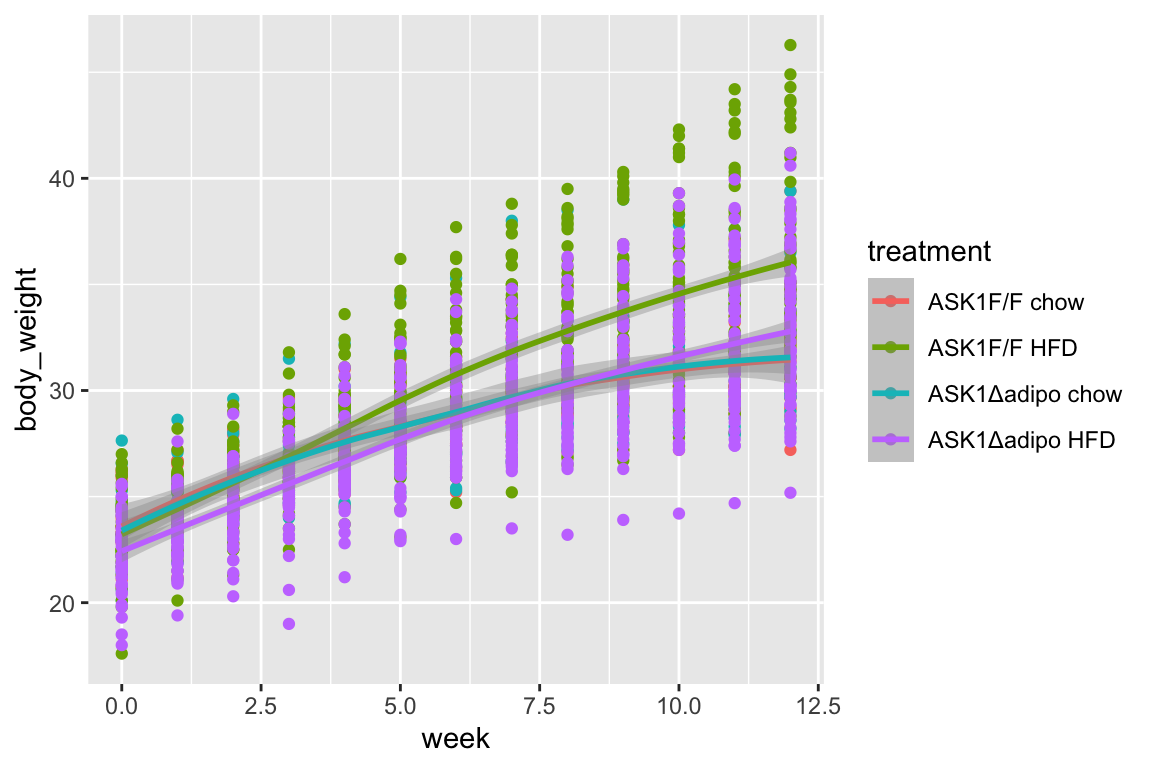
\includegraphics{Walker-elementary-statistical-modeling-draft_files/figure-latex/target-fig2b-initial-plot-2-1.pdf}
1. loess smooth. Growth in ASK1F/F + HFD clearly greater than other three treatment combinations.

\hypertarget{figure-2c-effect-of-ask1-ko-on-final-body-weight}{%
\section{Figure 2c -- Effect of ASK1 KO on final body weight}\label{figure-2c-effect-of-ask1-ko-on-final-body-weight}}

\hypertarget{figure-2c-import}{%
\subsection{Figure 2c -- import}\label{figure-2c-import}}

\begin{Shaded}
\begin{Highlighting}[]
\NormalTok{range_2c <-}\StringTok{ "A173:BD176"}
\NormalTok{y_cols <-}\StringTok{ }\KeywordTok{c}\NormalTok{(}\StringTok{"ASK1F/F chow"}\NormalTok{, }\StringTok{"ASK1Δadipo chow"}\NormalTok{, }\StringTok{"ASK1F/F HFD"}\NormalTok{, }\StringTok{"ASK1Δadipo HFD"}\NormalTok{)}
\NormalTok{fig_2c_import <-}\StringTok{ }\KeywordTok{read_excel}\NormalTok{(file_path,}
                     \DataTypeTok{sheet =}\NormalTok{ fig_}\DecValTok{2}\NormalTok{_sheet,}
                     \DataTypeTok{range =}\NormalTok{ range_2c,}
                     \DataTypeTok{col_names =} \OtherTok{FALSE}\NormalTok{) }\OperatorTok
\StringTok{  }\KeywordTok{transpose}\NormalTok{(}\DataTypeTok{make.names=}\DecValTok{1}\NormalTok{) }\OperatorTok
\StringTok{  }\KeywordTok{data.table}\NormalTok{() }\OperatorTok
\StringTok{  }\KeywordTok{melt}\NormalTok{(}\DataTypeTok{measure.vars =}\NormalTok{ y_cols,}
       \DataTypeTok{variable.name =} \StringTok{"treatment"}\NormalTok{,}
       \DataTypeTok{value.name =} \StringTok{"body_weight_gain"}\NormalTok{) }\OperatorTok
\StringTok{  }\KeywordTok{na.omit}\NormalTok{()}
\end{Highlighting}
\end{Shaded}

\begin{verbatim}
## New names:
## * `` -> ...1
## * `` -> ...2
## * `` -> ...3
## * `` -> ...4
## * `` -> ...5
## * ...
\end{verbatim}

\begin{Shaded}
\begin{Highlighting}[]
\NormalTok{fig_2c_import[, mouse_id }\OperatorTok{:}\ErrorTok{=}\StringTok{ }\KeywordTok{paste}\NormalTok{(treatment, .I, }\DataTypeTok{sep =} \StringTok{"_"}\NormalTok{),}
\NormalTok{       by =}\StringTok{ }\NormalTok{treatment]}
\end{Highlighting}
\end{Shaded}

\hypertarget{figure-2c-check-own-computation-of-weight-change-v-imported-value}{%
\subsection{Figure 2c -- check own computation of weight change v imported value}\label{figure-2c-check-own-computation-of-weight-change-v-imported-value}}

Note that three cases are missing from fig\_2c import that are in fig\_2b

\begin{Shaded}
\begin{Highlighting}[]
\CommentTok{# change colnames to char}
\NormalTok{fig_2c <-}\StringTok{ }\KeywordTok{copy}\NormalTok{(fig_2b_wide)}
\NormalTok{weeks <-}\StringTok{ }\KeywordTok{unique}\NormalTok{(fig_2b[, week])}
\KeywordTok{setnames}\NormalTok{(fig_2c,}
         \DataTypeTok{old =} \KeywordTok{colnames}\NormalTok{(fig_2c),}
         \DataTypeTok{new =} \KeywordTok{c}\NormalTok{(}\StringTok{"treatment"}\NormalTok{, }\KeywordTok{paste0}\NormalTok{(}\StringTok{"week_"}\NormalTok{, weeks), }\StringTok{"mouse_id"}\NormalTok{))}
\NormalTok{fig_2c[, weight_gain }\OperatorTok{:}\ErrorTok{=}\StringTok{ }\NormalTok{week_}\DecValTok{12} \OperatorTok{-}\StringTok{ }\NormalTok{week_}\DecValTok{0}\NormalTok{]}
\NormalTok{fig_2c <-}\StringTok{ }\NormalTok{fig_2c[, .SD, .SDcols =}\StringTok{ }\KeywordTok{c}\NormalTok{(}\StringTok{"treatment"}\NormalTok{,}
                                \StringTok{"week_0"}\NormalTok{,}
                                \StringTok{"week_12"}\NormalTok{,}
                                \StringTok{"weight_gain"}\NormalTok{)]}
\NormalTok{fig_2c[, mouse_id }\OperatorTok{:}\ErrorTok{=}\StringTok{ }\KeywordTok{paste}\NormalTok{(treatment, .I, }\DataTypeTok{sep =} \StringTok{"_"}\NormalTok{),}
\NormalTok{       by =}\StringTok{ }\NormalTok{treatment]}

\NormalTok{fig_2c[, }\KeywordTok{c}\NormalTok{(}\StringTok{"ask1"}\NormalTok{, }\StringTok{"diet"}\NormalTok{) }\OperatorTok{:}\ErrorTok{=}\StringTok{ }\KeywordTok{tstrsplit}\NormalTok{(treatment, }\StringTok{" "}\NormalTok{, }\DataTypeTok{fixed=}\OtherTok{TRUE}\NormalTok{)]}

\NormalTok{fig_2c_check <-}\StringTok{ }\KeywordTok{merge}\NormalTok{(fig_2c,}
\NormalTok{                fig_2c_import,}
                \DataTypeTok{by =} \KeywordTok{c}\NormalTok{(}\StringTok{"mouse_id"}\NormalTok{),}
                \DataTypeTok{all =} \OtherTok{TRUE}\NormalTok{)}

\CommentTok{#View(fig_2c_check)}
\end{Highlighting}
\end{Shaded}

\hypertarget{figure-2c-exploratory-plots}{%
\subsection{Figure 2c -- exploratory plots}\label{figure-2c-exploratory-plots}}

\begin{Shaded}
\begin{Highlighting}[]
\KeywordTok{qplot}\NormalTok{(}\DataTypeTok{x =}\NormalTok{ treatment,}
      \DataTypeTok{y =}\NormalTok{ weight_gain,}
      \DataTypeTok{data =}\NormalTok{ fig_2c)}
\end{Highlighting}
\end{Shaded}

\begin{verbatim}
## Warning in grid.Call(C_textBounds, as.graphicsAnnot(x$label), x$x, x$y, :
## conversion failure on 'ASK1Δadipo chow' in 'mbcsToSbcs': dot substituted
## for <ce>
\end{verbatim}

\begin{verbatim}
## Warning in grid.Call(C_textBounds, as.graphicsAnnot(x$label), x$x, x$y, :
## conversion failure on 'ASK1Δadipo chow' in 'mbcsToSbcs': dot substituted
## for <94>
\end{verbatim}

\begin{verbatim}
## Warning in grid.Call(C_textBounds, as.graphicsAnnot(x$label), x$x, x$y, :
## conversion failure on 'ASK1Δadipo HFD' in 'mbcsToSbcs': dot substituted for
## <ce>
\end{verbatim}

\begin{verbatim}
## Warning in grid.Call(C_textBounds, as.graphicsAnnot(x$label), x$x, x$y, :
## conversion failure on 'ASK1Δadipo HFD' in 'mbcsToSbcs': dot substituted for
## <94>
\end{verbatim}

\begin{verbatim}
## Warning in grid.Call(C_textBounds, as.graphicsAnnot(x$label), x$x, x$y, :
## conversion failure on 'ASK1Δadipo chow' in 'mbcsToSbcs': dot substituted
## for <ce>
\end{verbatim}

\begin{verbatim}
## Warning in grid.Call(C_textBounds, as.graphicsAnnot(x$label), x$x, x$y, :
## conversion failure on 'ASK1Δadipo chow' in 'mbcsToSbcs': dot substituted
## for <94>
\end{verbatim}

\begin{verbatim}
## Warning in grid.Call(C_textBounds, as.graphicsAnnot(x$label), x$x, x$y, :
## conversion failure on 'ASK1Δadipo HFD' in 'mbcsToSbcs': dot substituted for
## <ce>
\end{verbatim}

\begin{verbatim}
## Warning in grid.Call(C_textBounds, as.graphicsAnnot(x$label), x$x, x$y, :
## conversion failure on 'ASK1Δadipo HFD' in 'mbcsToSbcs': dot substituted for
## <94>
\end{verbatim}

\begin{verbatim}
## Warning in grid.Call(C_textBounds, as.graphicsAnnot(x$label), x$x, x$y, :
## conversion failure on 'ASK1Δadipo chow' in 'mbcsToSbcs': dot substituted
## for <ce>
\end{verbatim}

\begin{verbatim}
## Warning in grid.Call(C_textBounds, as.graphicsAnnot(x$label), x$x, x$y, :
## conversion failure on 'ASK1Δadipo chow' in 'mbcsToSbcs': dot substituted
## for <94>
\end{verbatim}

\begin{verbatim}
## Warning in grid.Call(C_textBounds, as.graphicsAnnot(x$label), x$x, x$y, :
## conversion failure on 'ASK1Δadipo HFD' in 'mbcsToSbcs': dot substituted for
## <ce>
\end{verbatim}

\begin{verbatim}
## Warning in grid.Call(C_textBounds, as.graphicsAnnot(x$label), x$x, x$y, :
## conversion failure on 'ASK1Δadipo HFD' in 'mbcsToSbcs': dot substituted for
## <94>
\end{verbatim}

\begin{verbatim}
## Warning in grid.Call(C_textBounds, as.graphicsAnnot(x$label), x$x, x$y, :
## conversion failure on 'ASK1Δadipo chow' in 'mbcsToSbcs': dot substituted
## for <ce>
\end{verbatim}

\begin{verbatim}
## Warning in grid.Call(C_textBounds, as.graphicsAnnot(x$label), x$x, x$y, :
## conversion failure on 'ASK1Δadipo chow' in 'mbcsToSbcs': dot substituted
## for <94>
\end{verbatim}

\begin{verbatim}
## Warning in grid.Call(C_textBounds, as.graphicsAnnot(x$label), x$x, x$y, :
## conversion failure on 'ASK1Δadipo HFD' in 'mbcsToSbcs': dot substituted for
## <ce>
\end{verbatim}

\begin{verbatim}
## Warning in grid.Call(C_textBounds, as.graphicsAnnot(x$label), x$x, x$y, :
## conversion failure on 'ASK1Δadipo HFD' in 'mbcsToSbcs': dot substituted for
## <94>
\end{verbatim}

\begin{verbatim}
## Warning in grid.Call(C_textBounds, as.graphicsAnnot(x$label), x$x, x$y, :
## conversion failure on 'ASK1Δadipo chow' in 'mbcsToSbcs': dot substituted
## for <ce>
\end{verbatim}

\begin{verbatim}
## Warning in grid.Call(C_textBounds, as.graphicsAnnot(x$label), x$x, x$y, :
## conversion failure on 'ASK1Δadipo chow' in 'mbcsToSbcs': dot substituted
## for <94>
\end{verbatim}

\begin{verbatim}
## Warning in grid.Call(C_textBounds, as.graphicsAnnot(x$label), x$x, x$y, :
## conversion failure on 'ASK1Δadipo HFD' in 'mbcsToSbcs': dot substituted for
## <ce>
\end{verbatim}

\begin{verbatim}
## Warning in grid.Call(C_textBounds, as.graphicsAnnot(x$label), x$x, x$y, :
## conversion failure on 'ASK1Δadipo HFD' in 'mbcsToSbcs': dot substituted for
## <94>
\end{verbatim}

\begin{verbatim}
## Warning in grid.Call(C_textBounds, as.graphicsAnnot(x$label), x$x, x$y, :
## conversion failure on 'ASK1Δadipo chow' in 'mbcsToSbcs': dot substituted
## for <ce>
\end{verbatim}

\begin{verbatim}
## Warning in grid.Call(C_textBounds, as.graphicsAnnot(x$label), x$x, x$y, :
## conversion failure on 'ASK1Δadipo chow' in 'mbcsToSbcs': dot substituted
## for <94>
\end{verbatim}

\begin{verbatim}
## Warning in grid.Call(C_textBounds, as.graphicsAnnot(x$label), x$x, x$y, :
## conversion failure on 'ASK1Δadipo HFD' in 'mbcsToSbcs': dot substituted for
## <ce>
\end{verbatim}

\begin{verbatim}
## Warning in grid.Call(C_textBounds, as.graphicsAnnot(x$label), x$x, x$y, :
## conversion failure on 'ASK1Δadipo HFD' in 'mbcsToSbcs': dot substituted for
## <94>
\end{verbatim}

\begin{verbatim}
## Warning in grid.Call(C_textBounds, as.graphicsAnnot(x$label), x$x, x$y, :
## conversion failure on 'ASK1Δadipo chow' in 'mbcsToSbcs': dot substituted
## for <ce>
\end{verbatim}

\begin{verbatim}
## Warning in grid.Call(C_textBounds, as.graphicsAnnot(x$label), x$x, x$y, :
## conversion failure on 'ASK1Δadipo chow' in 'mbcsToSbcs': dot substituted
## for <94>
\end{verbatim}

\begin{verbatim}
## Warning in grid.Call(C_textBounds, as.graphicsAnnot(x$label), x$x, x$y, :
## conversion failure on 'ASK1Δadipo HFD' in 'mbcsToSbcs': dot substituted for
## <ce>
\end{verbatim}

\begin{verbatim}
## Warning in grid.Call(C_textBounds, as.graphicsAnnot(x$label), x$x, x$y, :
## conversion failure on 'ASK1Δadipo HFD' in 'mbcsToSbcs': dot substituted for
## <94>
\end{verbatim}

\begin{verbatim}
## Warning in grid.Call(C_textBounds, as.graphicsAnnot(x$label), x$x, x$y, :
## conversion failure on 'ASK1Δadipo chow' in 'mbcsToSbcs': dot substituted
## for <ce>
\end{verbatim}

\begin{verbatim}
## Warning in grid.Call(C_textBounds, as.graphicsAnnot(x$label), x$x, x$y, :
## conversion failure on 'ASK1Δadipo chow' in 'mbcsToSbcs': dot substituted
## for <94>
\end{verbatim}

\begin{verbatim}
## Warning in grid.Call(C_textBounds, as.graphicsAnnot(x$label), x$x, x$y, :
## conversion failure on 'ASK1Δadipo HFD' in 'mbcsToSbcs': dot substituted for
## <ce>
\end{verbatim}

\begin{verbatim}
## Warning in grid.Call(C_textBounds, as.graphicsAnnot(x$label), x$x, x$y, :
## conversion failure on 'ASK1Δadipo HFD' in 'mbcsToSbcs': dot substituted for
## <94>
\end{verbatim}

\begin{verbatim}
## Warning in grid.Call(C_textBounds, as.graphicsAnnot(x$label), x$x, x$y, :
## conversion failure on 'ASK1Δadipo chow' in 'mbcsToSbcs': dot substituted
## for <ce>
\end{verbatim}

\begin{verbatim}
## Warning in grid.Call(C_textBounds, as.graphicsAnnot(x$label), x$x, x$y, :
## conversion failure on 'ASK1Δadipo chow' in 'mbcsToSbcs': dot substituted
## for <94>
\end{verbatim}

\begin{verbatim}
## Warning in grid.Call(C_textBounds, as.graphicsAnnot(x$label), x$x, x$y, :
## conversion failure on 'ASK1Δadipo HFD' in 'mbcsToSbcs': dot substituted for
## <ce>
\end{verbatim}

\begin{verbatim}
## Warning in grid.Call(C_textBounds, as.graphicsAnnot(x$label), x$x, x$y, :
## conversion failure on 'ASK1Δadipo HFD' in 'mbcsToSbcs': dot substituted for
## <94>
\end{verbatim}

\begin{verbatim}
## Warning in grid.Call(C_textBounds, as.graphicsAnnot(x$label), x$x, x$y, :
## conversion failure on 'ASK1Δadipo chow' in 'mbcsToSbcs': dot substituted
## for <ce>
\end{verbatim}

\begin{verbatim}
## Warning in grid.Call(C_textBounds, as.graphicsAnnot(x$label), x$x, x$y, :
## conversion failure on 'ASK1Δadipo chow' in 'mbcsToSbcs': dot substituted
## for <94>
\end{verbatim}

\begin{verbatim}
## Warning in grid.Call(C_textBounds, as.graphicsAnnot(x$label), x$x, x$y, :
## conversion failure on 'ASK1Δadipo HFD' in 'mbcsToSbcs': dot substituted for
## <ce>
\end{verbatim}

\begin{verbatim}
## Warning in grid.Call(C_textBounds, as.graphicsAnnot(x$label), x$x, x$y, :
## conversion failure on 'ASK1Δadipo HFD' in 'mbcsToSbcs': dot substituted for
## <94>
\end{verbatim}

\begin{verbatim}
## Warning in grid.Call(C_textBounds, as.graphicsAnnot(x$label), x$x, x$y, :
## conversion failure on 'ASK1Δadipo chow' in 'mbcsToSbcs': dot substituted
## for <ce>
\end{verbatim}

\begin{verbatim}
## Warning in grid.Call(C_textBounds, as.graphicsAnnot(x$label), x$x, x$y, :
## conversion failure on 'ASK1Δadipo chow' in 'mbcsToSbcs': dot substituted
## for <94>
\end{verbatim}

\begin{verbatim}
## Warning in grid.Call(C_textBounds, as.graphicsAnnot(x$label), x$x, x$y, :
## conversion failure on 'ASK1Δadipo HFD' in 'mbcsToSbcs': dot substituted for
## <ce>
\end{verbatim}

\begin{verbatim}
## Warning in grid.Call(C_textBounds, as.graphicsAnnot(x$label), x$x, x$y, :
## conversion failure on 'ASK1Δadipo HFD' in 'mbcsToSbcs': dot substituted for
## <94>
\end{verbatim}

\begin{verbatim}
## Warning in grid.Call(C_textBounds, as.graphicsAnnot(x$label), x$x, x$y, :
## conversion failure on 'ASK1Δadipo chow' in 'mbcsToSbcs': dot substituted
## for <ce>
\end{verbatim}

\begin{verbatim}
## Warning in grid.Call(C_textBounds, as.graphicsAnnot(x$label), x$x, x$y, :
## conversion failure on 'ASK1Δadipo chow' in 'mbcsToSbcs': dot substituted
## for <94>
\end{verbatim}

\begin{verbatim}
## Warning in grid.Call(C_textBounds, as.graphicsAnnot(x$label), x$x, x$y, :
## conversion failure on 'ASK1Δadipo HFD' in 'mbcsToSbcs': dot substituted for
## <ce>
\end{verbatim}

\begin{verbatim}
## Warning in grid.Call(C_textBounds, as.graphicsAnnot(x$label), x$x, x$y, :
## conversion failure on 'ASK1Δadipo HFD' in 'mbcsToSbcs': dot substituted for
## <94>
\end{verbatim}

\begin{verbatim}
## Warning in grid.Call(C_textBounds, as.graphicsAnnot(x$label), x$x, x$y, :
## conversion failure on 'ASK1Δadipo chow' in 'mbcsToSbcs': dot substituted
## for <ce>
\end{verbatim}

\begin{verbatim}
## Warning in grid.Call(C_textBounds, as.graphicsAnnot(x$label), x$x, x$y, :
## conversion failure on 'ASK1Δadipo chow' in 'mbcsToSbcs': dot substituted
## for <94>
\end{verbatim}

\begin{verbatim}
## Warning in grid.Call(C_textBounds, as.graphicsAnnot(x$label), x$x, x$y, :
## conversion failure on 'ASK1Δadipo HFD' in 'mbcsToSbcs': dot substituted for
## <ce>
\end{verbatim}

\begin{verbatim}
## Warning in grid.Call(C_textBounds, as.graphicsAnnot(x$label), x$x, x$y, :
## conversion failure on 'ASK1Δadipo HFD' in 'mbcsToSbcs': dot substituted for
## <94>
\end{verbatim}

\begin{verbatim}
## Warning in grid.Call.graphics(C_text, as.graphicsAnnot(x$label), x$x,
## x$y, : conversion failure on 'ASK1Δadipo chow' in 'mbcsToSbcs': dot
## substituted for <ce>
\end{verbatim}

\begin{verbatim}
## Warning in grid.Call.graphics(C_text, as.graphicsAnnot(x$label), x$x,
## x$y, : conversion failure on 'ASK1Δadipo chow' in 'mbcsToSbcs': dot
## substituted for <94>
\end{verbatim}

\begin{verbatim}
## Warning in grid.Call.graphics(C_text, as.graphicsAnnot(x$label), x$x,
## x$y, : conversion failure on 'ASK1Δadipo HFD' in 'mbcsToSbcs': dot
## substituted for <ce>
\end{verbatim}

\begin{verbatim}
## Warning in grid.Call.graphics(C_text, as.graphicsAnnot(x$label), x$x,
## x$y, : conversion failure on 'ASK1Δadipo HFD' in 'mbcsToSbcs': dot
## substituted for <94>
\end{verbatim}

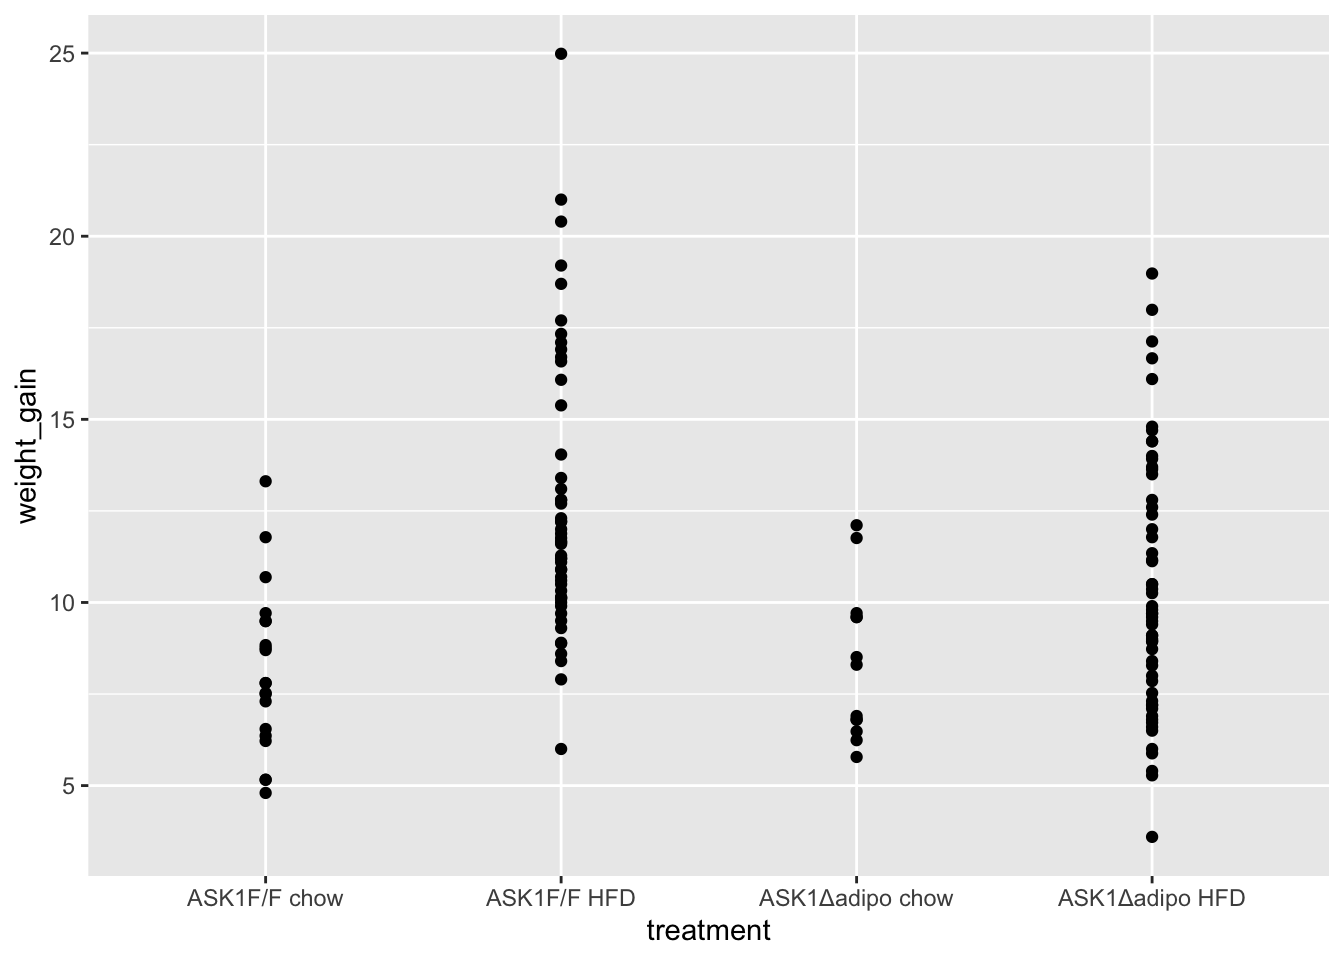
\includegraphics{Walker-elementary-statistical-modeling-draft_files/figure-latex/unnamed-chunk-3-1.pdf}

\begin{itemize}
\tightlist
\item
  no obvious outliers
\item
  variance increases with mean, as expected from growth, suggests a multiplicative model. But start with simple lm.
\end{itemize}

\hypertarget{figure-2c-fit-the-model-m1-lm}{%
\subsection{Figure 2c -- fit the model: m1 (lm)}\label{figure-2c-fit-the-model-m1-lm}}

\begin{Shaded}
\begin{Highlighting}[]
\NormalTok{fig_2c_m1 <-}\StringTok{ }\KeywordTok{lm}\NormalTok{(weight_gain }\OperatorTok{~}\StringTok{ }\NormalTok{week_}\DecValTok{0} \OperatorTok{+}\StringTok{ }\NormalTok{ask1}\OperatorTok{*}\NormalTok{diet, }\DataTypeTok{data =}\NormalTok{ fig_2c)}
\end{Highlighting}
\end{Shaded}

\hypertarget{figure-2c-check-the-model-m1}{%
\subsection{Figure 2c -- check the model: m1}\label{figure-2c-check-the-model-m1}}

\begin{Shaded}
\begin{Highlighting}[]
\CommentTok{# check normality assumption}
\KeywordTok{set.seed}\NormalTok{(}\DecValTok{1}\NormalTok{)}
\KeywordTok{qqPlot}\NormalTok{(fig_2c_m1, }\DataTypeTok{id=}\OtherTok{FALSE}\NormalTok{)}
\end{Highlighting}
\end{Shaded}

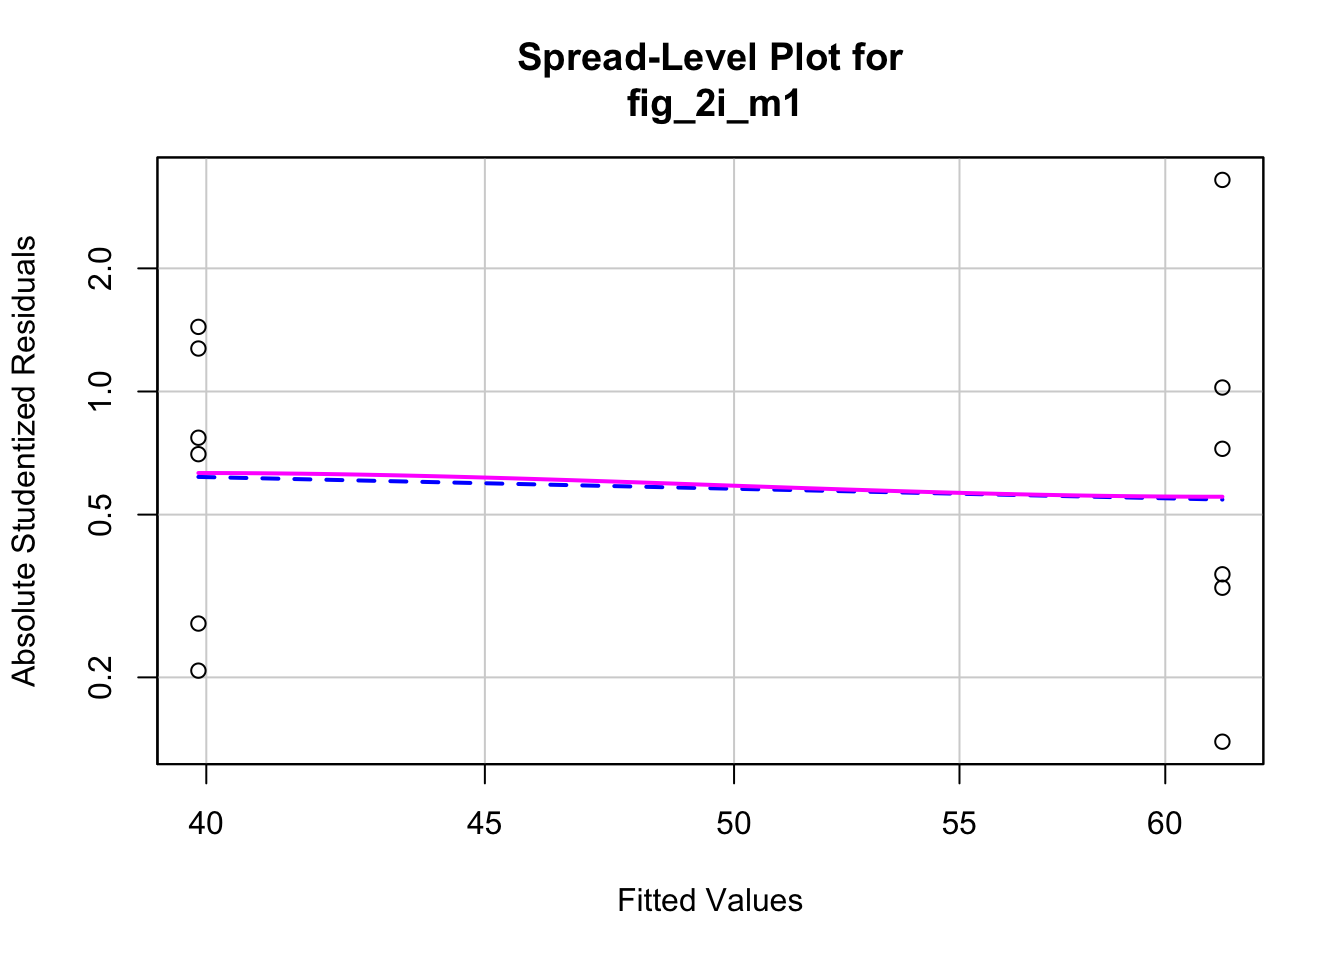
\includegraphics{Walker-elementary-statistical-modeling-draft_files/figure-latex/unnamed-chunk-5-1.pdf}

\begin{Shaded}
\begin{Highlighting}[]
\KeywordTok{spreadLevelPlot}\NormalTok{(fig_2c_m1, }\DataTypeTok{id=}\OtherTok{FALSE}\NormalTok{)}
\end{Highlighting}
\end{Shaded}

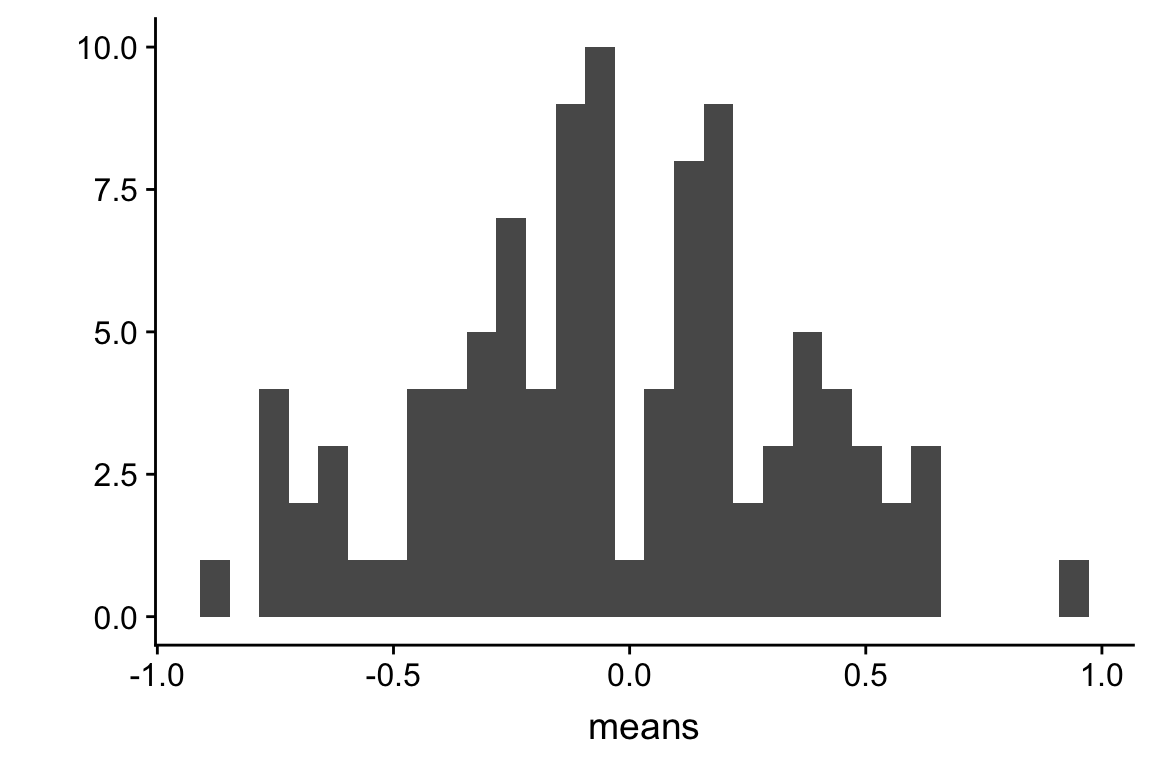
\includegraphics{Walker-elementary-statistical-modeling-draft_files/figure-latex/unnamed-chunk-6-1.pdf}

\begin{verbatim}
## 
## Suggested power transformation:  0.06419448
\end{verbatim}

\begin{itemize}
\tightlist
\item
  QQ indicates possible right skew but especially left side is squashed toward mean
\item
  spread-level indicates variance increases with mean
\end{itemize}

For p-value, this may not be too severe but for intervals, best to account for this. Try gamma with log link (which makes biological sense for growth)

\hypertarget{figure-2c-fit-the-model-m2-gamma-glm}{%
\subsection{Figure 2c -- fit the model: m2 (gamma glm)}\label{figure-2c-fit-the-model-m2-gamma-glm}}

\begin{Shaded}
\begin{Highlighting}[]
\NormalTok{fig_2c_m2 <-}\StringTok{ }\KeywordTok{glm}\NormalTok{(weight_gain }\OperatorTok{~}\StringTok{ }\NormalTok{week_}\DecValTok{0} \OperatorTok{+}\StringTok{ }\NormalTok{ask1}\OperatorTok{*}\NormalTok{diet,}
          \DataTypeTok{family =} \KeywordTok{Gamma}\NormalTok{(}\DataTypeTok{link =} \StringTok{"log"}\NormalTok{),}
          \DataTypeTok{data =}\NormalTok{ fig_2c)}
\end{Highlighting}
\end{Shaded}

\hypertarget{figure-2c-check-the-model-m2}{%
\subsection{Figure 2c -- check the model, m2}\label{figure-2c-check-the-model-m2}}

\begin{Shaded}
\begin{Highlighting}[]
\KeywordTok{set.seed}\NormalTok{(}\DecValTok{1}\NormalTok{)}
\NormalTok{fig_2c_m2_sim  <-}\StringTok{  }\KeywordTok{simulateResiduals}\NormalTok{(fig_2c_m2,  }\DataTypeTok{n=}\DecValTok{250}\NormalTok{)}
\end{Highlighting}
\end{Shaded}

\begin{verbatim}
## Model family was recognized or set as continuous, but duplicate values were detected in the response. Consider if you are fitting an appropriate model.
\end{verbatim}

\begin{Shaded}
\begin{Highlighting}[]
\KeywordTok{plot}\NormalTok{(fig_2c_m2_sim) }
\end{Highlighting}
\end{Shaded}

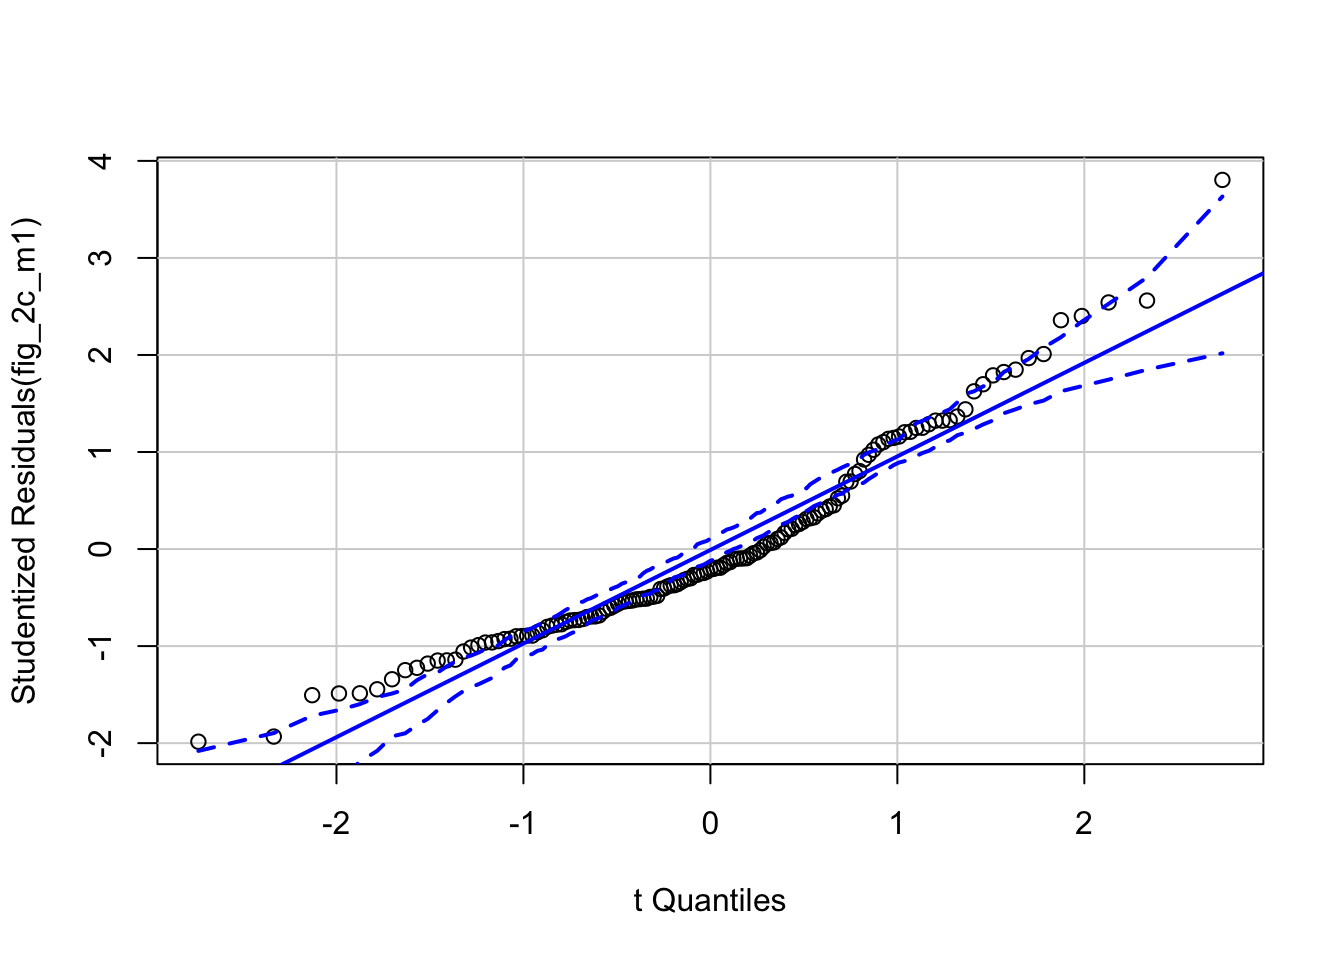
\includegraphics{Walker-elementary-statistical-modeling-draft_files/figure-latex/unnamed-chunk-8-1.pdf}

\begin{itemize}
\tightlist
\item
  well behaved QQ and spread-level
\end{itemize}

\hypertarget{figure-2c-inference-from-the-model}{%
\subsection{Figure 2c -- inference from the model}\label{figure-2c-inference-from-the-model}}

\begin{Shaded}
\begin{Highlighting}[]
\NormalTok{coef_table <-}\StringTok{ }\KeywordTok{cbind}\NormalTok{(}\KeywordTok{coef}\NormalTok{(}\KeywordTok{summary}\NormalTok{(fig_2c_m2)),}
                    \KeywordTok{exp}\NormalTok{(}\KeywordTok{confint}\NormalTok{(fig_2c_m2))) }\OperatorTok
\StringTok{  }\KeywordTok{data.table}\NormalTok{(}\DataTypeTok{keep.rownames =} \OtherTok{TRUE}\NormalTok{)}
\NormalTok{coef_table[, Estimate}\OperatorTok{:}\ErrorTok{=}\KeywordTok{exp}\NormalTok{(Estimate)]}
\NormalTok{knitr}\OperatorTok{::}\KeywordTok{kable}\NormalTok{(coef_table, }\DataTypeTok{digits =} \KeywordTok{c}\NormalTok{(}\DecValTok{0}\NormalTok{,}\DecValTok{2}\NormalTok{,}\DecValTok{2}\NormalTok{,}\DecValTok{2}\NormalTok{,}\DecValTok{4}\NormalTok{,}\DecValTok{2}\NormalTok{,}\DecValTok{2}\NormalTok{))}
\end{Highlighting}
\end{Shaded}

rn

Estimate

Std. Error

t value

Pr(\textgreater\textbar t\textbar)

2.5 \%

97.5 \%

(Intercept)

10.87

0.35

6.83

0.0000

5.53

21.50

week\_0

0.99

0.01

-0.84

0.3997

0.96

1.02

ask1ASK1Δadipo

1.03

0.11

0.24

0.8138

0.83

1.28

dietHFD

1.56

0.08

5.45

0.0000

1.33

1.82

ask1ASK1Δadipo:dietHFD

0.79

0.13

-1.93

0.0551

0.61

1.00

\begin{Shaded}
\begin{Highlighting}[]
\NormalTok{fig_2c_m2_emm <-}\StringTok{ }\KeywordTok{emmeans}\NormalTok{(fig_2c_m2, }\DataTypeTok{specs =} \KeywordTok{c}\NormalTok{(}\StringTok{"diet"}\NormalTok{, }\StringTok{"ask1"}\NormalTok{),}
                         \DataTypeTok{type =} \StringTok{"response"}\NormalTok{)}
\NormalTok{fig_2c_m2_pairs <-}\StringTok{ }\KeywordTok{contrast}\NormalTok{(fig_2c_m2_emm,}
                     \DataTypeTok{method =} \StringTok{"revpairwise"}\NormalTok{,}
                     \DataTypeTok{simple =} \StringTok{"each"}\NormalTok{,}
                     \DataTypeTok{combine =} \OtherTok{TRUE}\NormalTok{,}
                     \DataTypeTok{adjust =} \StringTok{"none"}\NormalTok{) }\OperatorTok
\StringTok{  }\KeywordTok{summary}\NormalTok{(}\DataTypeTok{infer =} \OtherTok{TRUE}\NormalTok{)}
\end{Highlighting}
\end{Shaded}

\begin{Shaded}
\begin{Highlighting}[]
\NormalTok{fig_2c_m2_emm}
\end{Highlighting}
\end{Shaded}

\begin{verbatim}
##  diet ask1       response    SE  df asymp.LCL asymp.UCL
##  chow ASK1F/F        8.19 0.568 Inf      7.15      9.39
##  HFD  ASK1F/F       12.75 0.548 Inf     11.72     13.87
##  chow ASK1Δadipo     8.41 0.721 Inf      7.11      9.95
##  HFD  ASK1Δadipo    10.28 0.424 Inf      9.48     11.14
## 
## Confidence level used: 0.95 
## Intervals are back-transformed from the log scale
\end{verbatim}

\begin{Shaded}
\begin{Highlighting}[]
\NormalTok{fig_2c_m2_pairs}
\end{Highlighting}
\end{Shaded}

\begin{verbatim}
##  ask1       diet contrast             ratio     SE  df asymp.LCL asymp.UCL
##  ASK1F/F    .    HFD / chow           1.556 0.1263 Inf     1.328     1.825
##  ASK1Δadipo .    HFD / chow           1.222 0.1168 Inf     1.013     1.474
##  .          chow ASK1Δadipo / ASK1F/F 1.026 0.1127 Inf     0.828     1.273
##  .          HFD  ASK1Δadipo / ASK1F/F 0.806 0.0485 Inf     0.716     0.907
##  z.ratio p.value
##   5.453  <.0001 
##   2.097  0.0360 
##   0.236  0.8134 
##  -3.587  0.0003 
## 
## Confidence level used: 0.95 
## Intervals are back-transformed from the log scale 
## Tests are performed on the log scale
\end{verbatim}

\begin{itemize}
\tightlist
\item
  within ASK1 Cn, HFD mean is 1.6X chow mean
\item
  within ASK1 KO, HFD mean is 1.2X chow mean
\item
  within chow, ASK1 KO mean is 1.0X ASK1 Cn mean
\item
  within HFD, ASK1 KO mean is 0.86X ASK1 Cn mean
\end{itemize}

\begin{Shaded}
\begin{Highlighting}[]
\CommentTok{# same as interaction effect in coefficient table}
\KeywordTok{contrast}\NormalTok{(fig_2c_m2_emm, }\DataTypeTok{interaction =} \StringTok{"pairwise"}\NormalTok{, }\DataTypeTok{by =} \OtherTok{NULL}\NormalTok{) }\OperatorTok
\StringTok{  }\KeywordTok{summary}\NormalTok{(}\DataTypeTok{infer =} \OtherTok{TRUE}\NormalTok{)}
\end{Highlighting}
\end{Shaded}

\begin{verbatim}
##  diet_pairwise ask1_pairwise        ratio     SE  df asymp.LCL asymp.UCL
##  chow / HFD    ASK1F/F / ASK1Δadipo 0.785 0.0982 Inf     0.614         1
##  z.ratio p.value
##  -1.934  0.0531 
## 
## Confidence level used: 0.95 
## Intervals are back-transformed from the log scale 
## Tests are performed on the log scale
\end{verbatim}

\begin{itemize}
\tightlist
\item
  the reduction in weight gain in the ASK1 KO mice compared to ASK1 CN is 0.785X. Notice that p \textgreater{} 0.05.
\end{itemize}

\hypertarget{figure-2c-plot-the-model}{%
\subsection{Figure 2c -- plot the model}\label{figure-2c-plot-the-model}}

\begin{Shaded}
\begin{Highlighting}[]
\NormalTok{fig_2c_m2_emm_dt <-}\StringTok{ }\KeywordTok{summary}\NormalTok{(fig_2c_m2_emm) }\OperatorTok
\StringTok{  }\NormalTok{data.table}
\NormalTok{fig_2c_m2_pairs_dt <-}\StringTok{ }\KeywordTok{data.table}\NormalTok{(fig_2c_m2_pairs)}
\NormalTok{fig_2c_m2_pairs_dt[ , p_pretty }\OperatorTok{:}\ErrorTok{=}\StringTok{ }\KeywordTok{pvalString}\NormalTok{(p.value)]}

\NormalTok{dodge_width <-}\StringTok{ }\FloatTok{0.8} \CommentTok{# separation between groups}
\CommentTok{# get x positions of brackets for p-values}
\CommentTok{# requires looking at table and mentally figuring out}
\CommentTok{# Chow is at x = 1 and HFD is at x = 2}
\NormalTok{fig_2c_m2_pairs_dt[, group1 }\OperatorTok{:}\ErrorTok{=}\StringTok{ }\KeywordTok{c}\NormalTok{(}\DecValTok{1}\OperatorTok{-}\NormalTok{dodge_width}\OperatorTok{/}\DecValTok{4}\NormalTok{,}
                                 \DecValTok{1}\OperatorTok{+}\NormalTok{dodge_width}\OperatorTok{/}\DecValTok{4}\NormalTok{,}
                                 \DecValTok{1}\OperatorTok{-}\NormalTok{dodge_width}\OperatorTok{/}\DecValTok{4}\NormalTok{,}
                                 \DecValTok{2}\OperatorTok{-}\NormalTok{dodge_width}\OperatorTok{/}\DecValTok{4}\NormalTok{)]}
\NormalTok{fig_2c_m2_pairs_dt[, group2 }\OperatorTok{:}\ErrorTok{=}\StringTok{ }\KeywordTok{c}\NormalTok{(}\DecValTok{2}\OperatorTok{-}\NormalTok{dodge_width}\OperatorTok{/}\DecValTok{4}\NormalTok{,}
                                 \DecValTok{2}\OperatorTok{+}\NormalTok{dodge_width}\OperatorTok{/}\DecValTok{4}\NormalTok{,}
                                 \DecValTok{1}\OperatorTok{+}\NormalTok{dodge_width}\OperatorTok{/}\DecValTok{4}\NormalTok{,}
                                 \DecValTok{2}\OperatorTok{+}\NormalTok{dodge_width}\OperatorTok{/}\DecValTok{4}\NormalTok{)]}

\NormalTok{pd <-}\StringTok{ }\KeywordTok{position_dodge}\NormalTok{(}\DataTypeTok{width =}\NormalTok{ dodge_width)}
\NormalTok{fig_2c_gg <-}\StringTok{ }\KeywordTok{ggplot}\NormalTok{(}\DataTypeTok{data =}\NormalTok{ fig_2c,}
                    \KeywordTok{aes}\NormalTok{(}\DataTypeTok{x =}\NormalTok{ diet,}
                        \DataTypeTok{y =}\NormalTok{ weight_gain,}
                        \DataTypeTok{color =}\NormalTok{ ask1)) }\OperatorTok{+}
\StringTok{  }
\StringTok{  }\CommentTok{# points}
\StringTok{  }\KeywordTok{geom_sina}\NormalTok{(}\DataTypeTok{alpha =} \FloatTok{0.5}\NormalTok{,}
            \DataTypeTok{position =}\NormalTok{ pd) }\OperatorTok{+}
\StringTok{  }
\StringTok{  }\CommentTok{# plot means and CI}
\StringTok{  }\KeywordTok{geom_errorbar}\NormalTok{(}\DataTypeTok{data =}\NormalTok{ fig_2c_m2_emm_dt,}
                \KeywordTok{aes}\NormalTok{(}\DataTypeTok{y =}\NormalTok{ response,}
                    \DataTypeTok{ymin =}\NormalTok{ asymp.LCL,}
                    \DataTypeTok{ymax =}\NormalTok{ asymp.UCL,}
                    \DataTypeTok{color =}\NormalTok{ ask1),}
                \DataTypeTok{width =} \DecValTok{0}\NormalTok{,}
                \DataTypeTok{position =}\NormalTok{ pd}
\NormalTok{  ) }\OperatorTok{+}
\StringTok{  }
\StringTok{  }\KeywordTok{geom_point}\NormalTok{(}\DataTypeTok{data =}\NormalTok{ fig_2c_m2_emm_dt,}
             \KeywordTok{aes}\NormalTok{(}\DataTypeTok{y =}\NormalTok{ response,}
                 \DataTypeTok{color =}\NormalTok{ ask1),}
             \DataTypeTok{size =} \DecValTok{3}\NormalTok{,}
             \DataTypeTok{position =}\NormalTok{ pd}
\NormalTok{  ) }\OperatorTok{+}
\StringTok{  }
\StringTok{  }\CommentTok{# plot p-values (y positions are adjusted by eye)}
\StringTok{  }\KeywordTok{stat_pvalue_manual}\NormalTok{(fig_2c_m2_pairs_dt,}
                     \DataTypeTok{label =} \StringTok{"p_pretty"}\NormalTok{,}
                     \DataTypeTok{y.position=}\KeywordTok{c}\NormalTok{(}\FloatTok{28.5}\NormalTok{, }\DecValTok{31}\NormalTok{, }\DecValTok{26}\NormalTok{, }\DecValTok{26}\NormalTok{),}
                     \DataTypeTok{tip.length =} \FloatTok{0.01}\NormalTok{) }\OperatorTok{+}
\StringTok{  }
\StringTok{  }\CommentTok{# aesthetics}
\StringTok{  }\KeywordTok{ylab}\NormalTok{(}\StringTok{"Weight Gain"}\NormalTok{) }\OperatorTok{+}
\StringTok{  }\KeywordTok{scale_color_manual}\NormalTok{(}\DataTypeTok{values=}\NormalTok{pal_nature_mod,}
                     \DataTypeTok{name =} \OtherTok{NULL}\NormalTok{) }\OperatorTok{+}
\StringTok{  }\KeywordTok{theme_pubr}\NormalTok{() }\OperatorTok{+}
\StringTok{  }\KeywordTok{theme}\NormalTok{(}\DataTypeTok{legend.position=}\StringTok{"top"}\NormalTok{) }\OperatorTok{+}
\StringTok{  }\KeywordTok{theme}\NormalTok{(}\DataTypeTok{axis.title.x=}\KeywordTok{element_blank}\NormalTok{()) }\OperatorTok{+}
\StringTok{  }
\StringTok{  }\OtherTok{NULL}

\NormalTok{fig_2c_gg}
\end{Highlighting}
\end{Shaded}

\begin{verbatim}
## Warning in grid.Call(C_textBounds, as.graphicsAnnot(x$label), x$x, x$y, :
## conversion failure on 'ASK1Δadipo' in 'mbcsToSbcs': dot substituted for
## <ce>
\end{verbatim}

\begin{verbatim}
## Warning in grid.Call(C_textBounds, as.graphicsAnnot(x$label), x$x, x$y, :
## conversion failure on 'ASK1Δadipo' in 'mbcsToSbcs': dot substituted for
## <94>
\end{verbatim}

\begin{verbatim}
## Warning in grid.Call(C_textBounds, as.graphicsAnnot(x$label), x$x, x$y, :
## conversion failure on 'ASK1Δadipo' in 'mbcsToSbcs': dot substituted for
## <ce>
\end{verbatim}

\begin{verbatim}
## Warning in grid.Call(C_textBounds, as.graphicsAnnot(x$label), x$x, x$y, :
## conversion failure on 'ASK1Δadipo' in 'mbcsToSbcs': dot substituted for
## <94>
\end{verbatim}

\begin{verbatim}
## Warning in grid.Call(C_textBounds, as.graphicsAnnot(x$label), x$x, x$y, :
## conversion failure on 'ASK1Δadipo' in 'mbcsToSbcs': dot substituted for
## <ce>
\end{verbatim}

\begin{verbatim}
## Warning in grid.Call(C_textBounds, as.graphicsAnnot(x$label), x$x, x$y, :
## conversion failure on 'ASK1Δadipo' in 'mbcsToSbcs': dot substituted for
## <94>
\end{verbatim}

\begin{verbatim}
## Warning in grid.Call(C_textBounds, as.graphicsAnnot(x$label), x$x, x$y, :
## conversion failure on 'ASK1Δadipo' in 'mbcsToSbcs': dot substituted for
## <ce>
\end{verbatim}

\begin{verbatim}
## Warning in grid.Call(C_textBounds, as.graphicsAnnot(x$label), x$x, x$y, :
## conversion failure on 'ASK1Δadipo' in 'mbcsToSbcs': dot substituted for
## <94>
\end{verbatim}

\begin{verbatim}
## Warning in grid.Call(C_textBounds, as.graphicsAnnot(x$label), x$x, x$y, :
## conversion failure on 'ASK1Δadipo' in 'mbcsToSbcs': dot substituted for
## <ce>
\end{verbatim}

\begin{verbatim}
## Warning in grid.Call(C_textBounds, as.graphicsAnnot(x$label), x$x, x$y, :
## conversion failure on 'ASK1Δadipo' in 'mbcsToSbcs': dot substituted for
## <94>
\end{verbatim}

\begin{verbatim}
## Warning in grid.Call(C_textBounds, as.graphicsAnnot(x$label), x$x, x$y, :
## conversion failure on 'ASK1Δadipo' in 'mbcsToSbcs': dot substituted for
## <ce>
\end{verbatim}

\begin{verbatim}
## Warning in grid.Call(C_textBounds, as.graphicsAnnot(x$label), x$x, x$y, :
## conversion failure on 'ASK1Δadipo' in 'mbcsToSbcs': dot substituted for
## <94>
\end{verbatim}

\begin{verbatim}
## Warning in grid.Call(C_textBounds, as.graphicsAnnot(x$label), x$x, x$y, :
## conversion failure on 'ASK1Δadipo' in 'mbcsToSbcs': dot substituted for
## <ce>
\end{verbatim}

\begin{verbatim}
## Warning in grid.Call(C_textBounds, as.graphicsAnnot(x$label), x$x, x$y, :
## conversion failure on 'ASK1Δadipo' in 'mbcsToSbcs': dot substituted for
## <94>
\end{verbatim}

\begin{verbatim}
## Warning in grid.Call(C_textBounds, as.graphicsAnnot(x$label), x$x, x$y, :
## conversion failure on 'ASK1Δadipo' in 'mbcsToSbcs': dot substituted for
## <ce>
\end{verbatim}

\begin{verbatim}
## Warning in grid.Call(C_textBounds, as.graphicsAnnot(x$label), x$x, x$y, :
## conversion failure on 'ASK1Δadipo' in 'mbcsToSbcs': dot substituted for
## <94>
\end{verbatim}

\begin{verbatim}
## Warning in grid.Call(C_textBounds, as.graphicsAnnot(x$label), x$x, x$y, :
## conversion failure on 'ASK1Δadipo' in 'mbcsToSbcs': dot substituted for
## <ce>
\end{verbatim}

\begin{verbatim}
## Warning in grid.Call(C_textBounds, as.graphicsAnnot(x$label), x$x, x$y, :
## conversion failure on 'ASK1Δadipo' in 'mbcsToSbcs': dot substituted for
## <94>
\end{verbatim}

\begin{verbatim}
## Warning in grid.Call(C_textBounds, as.graphicsAnnot(x$label), x$x, x$y, :
## conversion failure on 'ASK1Δadipo' in 'mbcsToSbcs': dot substituted for
## <ce>
\end{verbatim}

\begin{verbatim}
## Warning in grid.Call(C_textBounds, as.graphicsAnnot(x$label), x$x, x$y, :
## conversion failure on 'ASK1Δadipo' in 'mbcsToSbcs': dot substituted for
## <94>
\end{verbatim}

\begin{verbatim}
## Warning in grid.Call(C_textBounds, as.graphicsAnnot(x$label), x$x, x$y, :
## conversion failure on 'ASK1Δadipo' in 'mbcsToSbcs': dot substituted for
## <ce>
\end{verbatim}

\begin{verbatim}
## Warning in grid.Call(C_textBounds, as.graphicsAnnot(x$label), x$x, x$y, :
## conversion failure on 'ASK1Δadipo' in 'mbcsToSbcs': dot substituted for
## <94>
\end{verbatim}

\begin{verbatim}
## Warning in grid.Call(C_textBounds, as.graphicsAnnot(x$label), x$x, x$y, :
## conversion failure on 'ASK1Δadipo' in 'mbcsToSbcs': dot substituted for
## <ce>
\end{verbatim}

\begin{verbatim}
## Warning in grid.Call(C_textBounds, as.graphicsAnnot(x$label), x$x, x$y, :
## conversion failure on 'ASK1Δadipo' in 'mbcsToSbcs': dot substituted for
## <94>
\end{verbatim}

\begin{verbatim}
## Warning in grid.Call(C_textBounds, as.graphicsAnnot(x$label), x$x, x$y, :
## conversion failure on 'ASK1Δadipo' in 'mbcsToSbcs': dot substituted for
## <ce>
\end{verbatim}

\begin{verbatim}
## Warning in grid.Call(C_textBounds, as.graphicsAnnot(x$label), x$x, x$y, :
## conversion failure on 'ASK1Δadipo' in 'mbcsToSbcs': dot substituted for
## <94>
\end{verbatim}

\begin{verbatim}
## Warning in grid.Call(C_textBounds, as.graphicsAnnot(x$label), x$x, x$y, :
## conversion failure on 'ASK1Δadipo' in 'mbcsToSbcs': dot substituted for
## <ce>
\end{verbatim}

\begin{verbatim}
## Warning in grid.Call(C_textBounds, as.graphicsAnnot(x$label), x$x, x$y, :
## conversion failure on 'ASK1Δadipo' in 'mbcsToSbcs': dot substituted for
## <94>
\end{verbatim}

\begin{verbatim}
## Warning in grid.Call(C_textBounds, as.graphicsAnnot(x$label), x$x, x$y, :
## conversion failure on 'ASK1Δadipo' in 'mbcsToSbcs': dot substituted for
## <ce>
\end{verbatim}

\begin{verbatim}
## Warning in grid.Call(C_textBounds, as.graphicsAnnot(x$label), x$x, x$y, :
## conversion failure on 'ASK1Δadipo' in 'mbcsToSbcs': dot substituted for
## <94>
\end{verbatim}

\begin{verbatim}
## Warning in grid.Call(C_textBounds, as.graphicsAnnot(x$label), x$x, x$y, :
## conversion failure on 'ASK1Δadipo' in 'mbcsToSbcs': dot substituted for
## <ce>
\end{verbatim}

\begin{verbatim}
## Warning in grid.Call(C_textBounds, as.graphicsAnnot(x$label), x$x, x$y, :
## conversion failure on 'ASK1Δadipo' in 'mbcsToSbcs': dot substituted for
## <94>
\end{verbatim}

\begin{verbatim}
## Warning in grid.Call(C_textBounds, as.graphicsAnnot(x$label), x$x, x$y, :
## conversion failure on 'ASK1Δadipo' in 'mbcsToSbcs': dot substituted for
## <ce>
\end{verbatim}

\begin{verbatim}
## Warning in grid.Call(C_textBounds, as.graphicsAnnot(x$label), x$x, x$y, :
## conversion failure on 'ASK1Δadipo' in 'mbcsToSbcs': dot substituted for
## <94>
\end{verbatim}

\begin{verbatim}
## Warning in grid.Call(C_textBounds, as.graphicsAnnot(x$label), x$x, x$y, :
## conversion failure on 'ASK1Δadipo' in 'mbcsToSbcs': dot substituted for
## <ce>
\end{verbatim}

\begin{verbatim}
## Warning in grid.Call(C_textBounds, as.graphicsAnnot(x$label), x$x, x$y, :
## conversion failure on 'ASK1Δadipo' in 'mbcsToSbcs': dot substituted for
## <94>
\end{verbatim}

\begin{verbatim}
## Warning in grid.Call(C_textBounds, as.graphicsAnnot(x$label), x$x, x$y, :
## conversion failure on 'ASK1Δadipo' in 'mbcsToSbcs': dot substituted for
## <ce>
\end{verbatim}

\begin{verbatim}
## Warning in grid.Call(C_textBounds, as.graphicsAnnot(x$label), x$x, x$y, :
## conversion failure on 'ASK1Δadipo' in 'mbcsToSbcs': dot substituted for
## <94>
\end{verbatim}

\begin{verbatim}
## Warning in grid.Call(C_textBounds, as.graphicsAnnot(x$label), x$x, x$y, :
## conversion failure on 'ASK1Δadipo' in 'mbcsToSbcs': dot substituted for
## <ce>
\end{verbatim}

\begin{verbatim}
## Warning in grid.Call(C_textBounds, as.graphicsAnnot(x$label), x$x, x$y, :
## conversion failure on 'ASK1Δadipo' in 'mbcsToSbcs': dot substituted for
## <94>
\end{verbatim}

\begin{verbatim}
## Warning in grid.Call(C_textBounds, as.graphicsAnnot(x$label), x$x, x$y, :
## conversion failure on 'ASK1Δadipo' in 'mbcsToSbcs': dot substituted for
## <ce>
\end{verbatim}

\begin{verbatim}
## Warning in grid.Call(C_textBounds, as.graphicsAnnot(x$label), x$x, x$y, :
## conversion failure on 'ASK1Δadipo' in 'mbcsToSbcs': dot substituted for
## <94>
\end{verbatim}

\begin{verbatim}
## Warning in grid.Call(C_textBounds, as.graphicsAnnot(x$label), x$x, x$y, :
## conversion failure on 'ASK1Δadipo' in 'mbcsToSbcs': dot substituted for
## <ce>
\end{verbatim}

\begin{verbatim}
## Warning in grid.Call(C_textBounds, as.graphicsAnnot(x$label), x$x, x$y, :
## conversion failure on 'ASK1Δadipo' in 'mbcsToSbcs': dot substituted for
## <94>
\end{verbatim}

\begin{verbatim}
## Warning in grid.Call(C_textBounds, as.graphicsAnnot(x$label), x$x, x$y, :
## conversion failure on 'ASK1Δadipo' in 'mbcsToSbcs': dot substituted for
## <ce>
\end{verbatim}

\begin{verbatim}
## Warning in grid.Call(C_textBounds, as.graphicsAnnot(x$label), x$x, x$y, :
## conversion failure on 'ASK1Δadipo' in 'mbcsToSbcs': dot substituted for
## <94>
\end{verbatim}

\begin{verbatim}
## Warning in grid.Call(C_textBounds, as.graphicsAnnot(x$label), x$x, x$y, :
## conversion failure on 'ASK1Δadipo' in 'mbcsToSbcs': dot substituted for
## <ce>
\end{verbatim}

\begin{verbatim}
## Warning in grid.Call(C_textBounds, as.graphicsAnnot(x$label), x$x, x$y, :
## conversion failure on 'ASK1Δadipo' in 'mbcsToSbcs': dot substituted for
## <94>
\end{verbatim}

\begin{verbatim}
## Warning in grid.Call.graphics(C_text, as.graphicsAnnot(x$label), x$x,
## x$y, : conversion failure on 'ASK1Δadipo' in 'mbcsToSbcs': dot substituted
## for <ce>
\end{verbatim}

\begin{verbatim}
## Warning in grid.Call.graphics(C_text, as.graphicsAnnot(x$label), x$x,
## x$y, : conversion failure on 'ASK1Δadipo' in 'mbcsToSbcs': dot substituted
## for <94>
\end{verbatim}

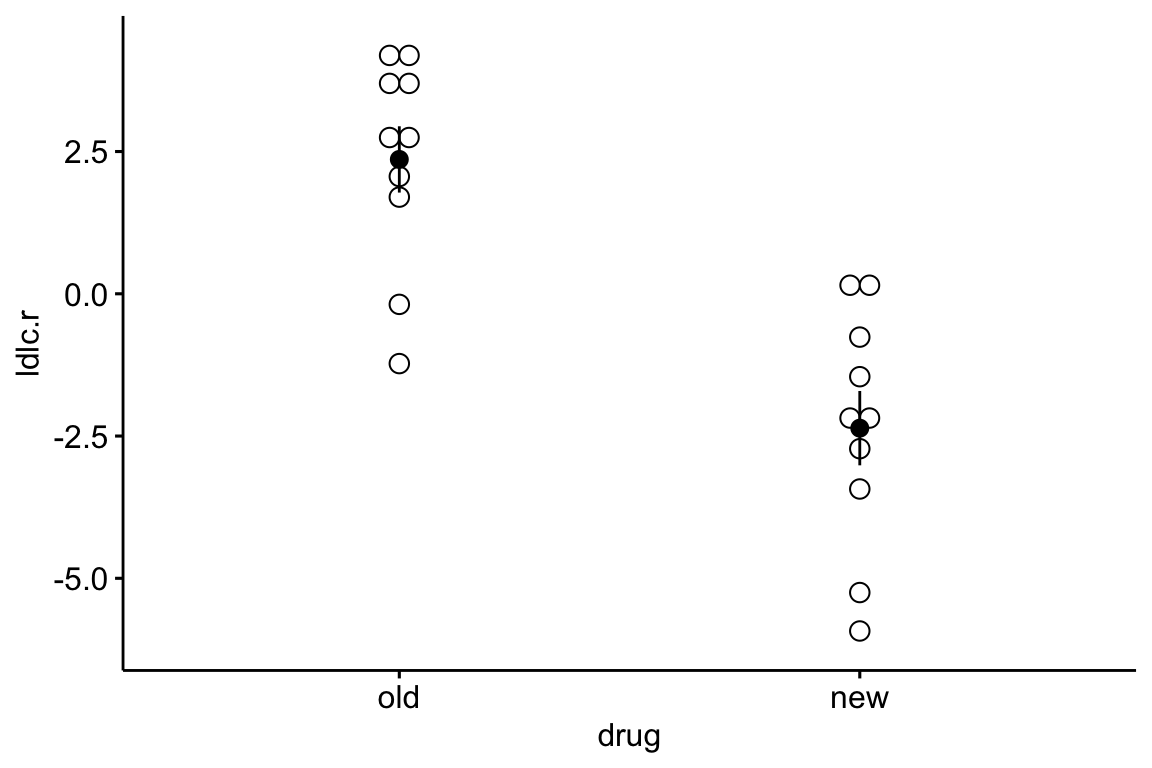
\includegraphics{Walker-elementary-statistical-modeling-draft_files/figure-latex/unnamed-chunk-14-1.pdf}

\hypertarget{figure-2c-report}{%
\subsection{Figure 2c -- report}\label{figure-2c-report}}

Results could be reported using either:

(This is inconsistent with plot, if using this, the plot should reverse what factor is on the x-axis and what factor is the grouping (color) variable) Mean weight gain in ASK1F/F mice on HFD was 1.56 (95\% CI: 1.33, 1.82, \(p < 0.0001\)) times that of ASK1F/F mice on chow while mean weight gain in ASK1Δadipo mice on HFD was only 1.22 (95\% CI: 1.01, 1.47, \(p = 0.036\)) times that of ASK1Δadipo mice on chow. This reduction in weight gain in ASK1Δadipo mice compared to ASK1F/F control mice was 0.79 times (95\% CI; 0.61, 1.00, \(p = 0.0531\)).

(This is consistent with the plot in that its comparing difference in the grouping factor within each level of the factor on the x-axis) Mean weight gain in ASK1Δadipo mice on chow was trivially larger (1.03 times) than that in ASK1F/F mice on chow (95\% CI: 0.83, 1.27, \(p = 0.81\)) while mean weight gain in ASK1Δadipo mice on HFD was smaller (0.81 times) than that in ASK1F/F control mice on HFD (95\% CI: 0.72 , 0.91, \(p = 0.0003\)). This reduction in weight gain in ASK1Δadipo mice compared to ASK1Δadipo mice is 0.79 times (95\% CI; 0.61, 1.00, \(p = 0.0531\)).

\textbf{note to research team}. The big difference in \emph{p}-values between weight difference on chow and weight difference on HFD might lead one to believe there is a ``difference in this difference''. Using a \emph{p}-value = effect strategy, this is not supported.

\hypertarget{figure-2d-effect-of-ask1-ko-on-glucose-tolerance-whole-curve}{%
\section{Figure 2d -- Effect of ASK1 KO on glucose tolerance (whole curve)}\label{figure-2d-effect-of-ask1-ko-on-glucose-tolerance-whole-curve}}

\hypertarget{figure-2d-import}{%
\subsection{Figure 2d -- Import}\label{figure-2d-import}}

\begin{Shaded}
\begin{Highlighting}[]
\NormalTok{range_list <-}\StringTok{ }\KeywordTok{c}\NormalTok{(}\StringTok{"A179:H189"}\NormalTok{, }\StringTok{"A191:H199"}\NormalTok{, }\StringTok{"A201:H214"}\NormalTok{, }\StringTok{"A216:H230"}\NormalTok{)}
\NormalTok{fig_2d_wide <-}\StringTok{ }\KeywordTok{data.table}\NormalTok{(}\OtherTok{NULL}\NormalTok{)}
\ControlFlowTok{for}\NormalTok{(range_i }\ControlFlowTok{in}\NormalTok{ range_list)\{}
\NormalTok{  part <-}\StringTok{ }\KeywordTok{import_fig_2_part}\NormalTok{(range_i)}
\NormalTok{  fig_2d_wide <-}\StringTok{ }\KeywordTok{rbind}\NormalTok{(fig_2d_wide,}
\NormalTok{                       part)}
\NormalTok{\}}
\NormalTok{fig_2d_wide[, }\KeywordTok{c}\NormalTok{(}\StringTok{"ask1"}\NormalTok{, }\StringTok{"diet"}\NormalTok{) }\OperatorTok{:}\ErrorTok{=}\StringTok{ }\KeywordTok{tstrsplit}\NormalTok{(treatment, }\StringTok{" "}\NormalTok{, }\DataTypeTok{fixed=}\OtherTok{TRUE}\NormalTok{)]}

\CommentTok{# melt}
\NormalTok{fig_2d <-}\StringTok{ }\KeywordTok{melt}\NormalTok{(fig_2d_wide,}
               \DataTypeTok{id.vars =} \KeywordTok{c}\NormalTok{(}\StringTok{"treatment"}\NormalTok{,}
                           \StringTok{"ask1"}\NormalTok{,}
                           \StringTok{"diet"}\NormalTok{,}
                           \StringTok{"mouse_id"}\NormalTok{),}
               \DataTypeTok{variable.name =} \StringTok{"time"}\NormalTok{,}
               \DataTypeTok{value.name =} \StringTok{"glucose"}\NormalTok{)}
\NormalTok{fig_2d[, time }\OperatorTok{:}\ErrorTok{=}\StringTok{ }\KeywordTok{as.numeric}\NormalTok{(}\KeywordTok{as.character}\NormalTok{(time))]}

\CommentTok{# for plot only (not analysis!)}
\NormalTok{shift <-}\StringTok{ }\DecValTok{2}
\NormalTok{fig_2d[treatment }\OperatorTok{==}\StringTok{ "ASK1F/F chow"}\NormalTok{, time_x }\OperatorTok{:}\ErrorTok{=}\StringTok{ }\NormalTok{time }\OperatorTok{-}\StringTok{ }\NormalTok{shift}\OperatorTok{*}\FloatTok{1.5}\NormalTok{]}
\NormalTok{fig_2d[treatment }\OperatorTok{==}\StringTok{ "ASK1Δadipo chow"}\NormalTok{, time_x }\OperatorTok{:}\ErrorTok{=}\StringTok{ }\NormalTok{time }\OperatorTok{-}\StringTok{ }\NormalTok{shift}\OperatorTok{*}\NormalTok{.}\DecValTok{5}\NormalTok{]}
\NormalTok{fig_2d[treatment }\OperatorTok{==}\StringTok{ "ASK1F/F HFD"}\NormalTok{, time_x }\OperatorTok{:}\ErrorTok{=}\StringTok{ }\NormalTok{time }\OperatorTok{+}\StringTok{ }\NormalTok{shift}\OperatorTok{*}\NormalTok{.}\DecValTok{5}\NormalTok{]}
\NormalTok{fig_2d[treatment }\OperatorTok{==}\StringTok{ "ASK1Δadipo HFD"}\NormalTok{, time_x }\OperatorTok{:}\ErrorTok{=}\StringTok{ }\NormalTok{time }\OperatorTok{+}\StringTok{ }\NormalTok{shift}\OperatorTok{*}\FloatTok{1.5}\NormalTok{]}
\end{Highlighting}
\end{Shaded}

\hypertarget{figure-2d-exploratory-plots}{%
\subsection{Figure 2d -- exploratory plots}\label{figure-2d-exploratory-plots}}

\begin{Shaded}
\begin{Highlighting}[]
\KeywordTok{qplot}\NormalTok{(}\DataTypeTok{x =}\NormalTok{ time_x, }\DataTypeTok{y =}\NormalTok{ glucose, }\DataTypeTok{color =}\NormalTok{ treatment, }\DataTypeTok{data =}\NormalTok{ fig_2d) }\OperatorTok{+}
\StringTok{  }\KeywordTok{geom_line}\NormalTok{(}\KeywordTok{aes}\NormalTok{(}\DataTypeTok{group =}\NormalTok{ mouse_id), }\DataTypeTok{alpha =} \FloatTok{0.3}\NormalTok{)}
\end{Highlighting}
\end{Shaded}

\begin{verbatim}
## Warning in grid.Call(C_textBounds, as.graphicsAnnot(x$label), x$x, x$y, :
## conversion failure on 'ASK1Δadipo chow' in 'mbcsToSbcs': dot substituted
## for <ce>
\end{verbatim}

\begin{verbatim}
## Warning in grid.Call(C_textBounds, as.graphicsAnnot(x$label), x$x, x$y, :
## conversion failure on 'ASK1Δadipo chow' in 'mbcsToSbcs': dot substituted
## for <94>
\end{verbatim}

\begin{verbatim}
## Warning in grid.Call(C_textBounds, as.graphicsAnnot(x$label), x$x, x$y, :
## conversion failure on 'ASK1Δadipo chow' in 'mbcsToSbcs': dot substituted
## for <ce>
\end{verbatim}

\begin{verbatim}
## Warning in grid.Call(C_textBounds, as.graphicsAnnot(x$label), x$x, x$y, :
## conversion failure on 'ASK1Δadipo chow' in 'mbcsToSbcs': dot substituted
## for <94>
\end{verbatim}

\begin{verbatim}
## Warning in grid.Call(C_textBounds, as.graphicsAnnot(x$label), x$x, x$y, :
## conversion failure on 'ASK1Δadipo chow' in 'mbcsToSbcs': dot substituted
## for <ce>
\end{verbatim}

\begin{verbatim}
## Warning in grid.Call(C_textBounds, as.graphicsAnnot(x$label), x$x, x$y, :
## conversion failure on 'ASK1Δadipo chow' in 'mbcsToSbcs': dot substituted
## for <94>
\end{verbatim}

\begin{verbatim}
## Warning in grid.Call(C_textBounds, as.graphicsAnnot(x$label), x$x, x$y, :
## conversion failure on 'ASK1Δadipo chow' in 'mbcsToSbcs': dot substituted
## for <ce>
\end{verbatim}

\begin{verbatim}
## Warning in grid.Call(C_textBounds, as.graphicsAnnot(x$label), x$x, x$y, :
## conversion failure on 'ASK1Δadipo chow' in 'mbcsToSbcs': dot substituted
## for <94>
\end{verbatim}

\begin{verbatim}
## Warning in grid.Call(C_textBounds, as.graphicsAnnot(x$label), x$x, x$y, :
## conversion failure on 'ASK1Δadipo chow' in 'mbcsToSbcs': dot substituted
## for <ce>
\end{verbatim}

\begin{verbatim}
## Warning in grid.Call(C_textBounds, as.graphicsAnnot(x$label), x$x, x$y, :
## conversion failure on 'ASK1Δadipo chow' in 'mbcsToSbcs': dot substituted
## for <94>
\end{verbatim}

\begin{verbatim}
## Warning in grid.Call(C_textBounds, as.graphicsAnnot(x$label), x$x, x$y, :
## conversion failure on 'ASK1Δadipo HFD' in 'mbcsToSbcs': dot substituted for
## <ce>
\end{verbatim}

\begin{verbatim}
## Warning in grid.Call(C_textBounds, as.graphicsAnnot(x$label), x$x, x$y, :
## conversion failure on 'ASK1Δadipo HFD' in 'mbcsToSbcs': dot substituted for
## <94>
\end{verbatim}

\begin{verbatim}
## Warning in grid.Call(C_textBounds, as.graphicsAnnot(x$label), x$x, x$y, :
## conversion failure on 'ASK1Δadipo HFD' in 'mbcsToSbcs': dot substituted for
## <ce>
\end{verbatim}

\begin{verbatim}
## Warning in grid.Call(C_textBounds, as.graphicsAnnot(x$label), x$x, x$y, :
## conversion failure on 'ASK1Δadipo HFD' in 'mbcsToSbcs': dot substituted for
## <94>
\end{verbatim}

\begin{verbatim}
## Warning in grid.Call(C_textBounds, as.graphicsAnnot(x$label), x$x, x$y, :
## conversion failure on 'ASK1Δadipo HFD' in 'mbcsToSbcs': dot substituted for
## <ce>
\end{verbatim}

\begin{verbatim}
## Warning in grid.Call(C_textBounds, as.graphicsAnnot(x$label), x$x, x$y, :
## conversion failure on 'ASK1Δadipo HFD' in 'mbcsToSbcs': dot substituted for
## <94>
\end{verbatim}

\begin{verbatim}
## Warning in grid.Call(C_textBounds, as.graphicsAnnot(x$label), x$x, x$y, :
## conversion failure on 'ASK1Δadipo HFD' in 'mbcsToSbcs': dot substituted for
## <ce>
\end{verbatim}

\begin{verbatim}
## Warning in grid.Call(C_textBounds, as.graphicsAnnot(x$label), x$x, x$y, :
## conversion failure on 'ASK1Δadipo HFD' in 'mbcsToSbcs': dot substituted for
## <94>
\end{verbatim}

\begin{verbatim}
## Warning in grid.Call(C_textBounds, as.graphicsAnnot(x$label), x$x, x$y, :
## conversion failure on 'ASK1Δadipo HFD' in 'mbcsToSbcs': dot substituted for
## <ce>
\end{verbatim}

\begin{verbatim}
## Warning in grid.Call(C_textBounds, as.graphicsAnnot(x$label), x$x, x$y, :
## conversion failure on 'ASK1Δadipo HFD' in 'mbcsToSbcs': dot substituted for
## <94>
\end{verbatim}

\begin{verbatim}
## Warning in grid.Call(C_textBounds, as.graphicsAnnot(x$label), x$x, x$y, :
## conversion failure on 'ASK1Δadipo chow' in 'mbcsToSbcs': dot substituted
## for <ce>
\end{verbatim}

\begin{verbatim}
## Warning in grid.Call(C_textBounds, as.graphicsAnnot(x$label), x$x, x$y, :
## conversion failure on 'ASK1Δadipo chow' in 'mbcsToSbcs': dot substituted
## for <94>
\end{verbatim}

\begin{verbatim}
## Warning in grid.Call(C_textBounds, as.graphicsAnnot(x$label), x$x, x$y, :
## conversion failure on 'ASK1Δadipo chow' in 'mbcsToSbcs': dot substituted
## for <ce>
\end{verbatim}

\begin{verbatim}
## Warning in grid.Call(C_textBounds, as.graphicsAnnot(x$label), x$x, x$y, :
## conversion failure on 'ASK1Δadipo chow' in 'mbcsToSbcs': dot substituted
## for <94>
\end{verbatim}

\begin{verbatim}
## Warning in grid.Call(C_textBounds, as.graphicsAnnot(x$label), x$x, x$y, :
## conversion failure on 'ASK1Δadipo chow' in 'mbcsToSbcs': dot substituted
## for <ce>
\end{verbatim}

\begin{verbatim}
## Warning in grid.Call(C_textBounds, as.graphicsAnnot(x$label), x$x, x$y, :
## conversion failure on 'ASK1Δadipo chow' in 'mbcsToSbcs': dot substituted
## for <94>
\end{verbatim}

\begin{verbatim}
## Warning in grid.Call(C_textBounds, as.graphicsAnnot(x$label), x$x, x$y, :
## conversion failure on 'ASK1Δadipo chow' in 'mbcsToSbcs': dot substituted
## for <ce>
\end{verbatim}

\begin{verbatim}
## Warning in grid.Call(C_textBounds, as.graphicsAnnot(x$label), x$x, x$y, :
## conversion failure on 'ASK1Δadipo chow' in 'mbcsToSbcs': dot substituted
## for <94>
\end{verbatim}

\begin{verbatim}
## Warning in grid.Call(C_textBounds, as.graphicsAnnot(x$label), x$x, x$y, :
## conversion failure on 'ASK1Δadipo chow' in 'mbcsToSbcs': dot substituted
## for <ce>
\end{verbatim}

\begin{verbatim}
## Warning in grid.Call(C_textBounds, as.graphicsAnnot(x$label), x$x, x$y, :
## conversion failure on 'ASK1Δadipo chow' in 'mbcsToSbcs': dot substituted
## for <94>
\end{verbatim}

\begin{verbatim}
## Warning in grid.Call(C_textBounds, as.graphicsAnnot(x$label), x$x, x$y, :
## conversion failure on 'ASK1Δadipo HFD' in 'mbcsToSbcs': dot substituted for
## <ce>
\end{verbatim}

\begin{verbatim}
## Warning in grid.Call(C_textBounds, as.graphicsAnnot(x$label), x$x, x$y, :
## conversion failure on 'ASK1Δadipo HFD' in 'mbcsToSbcs': dot substituted for
## <94>
\end{verbatim}

\begin{verbatim}
## Warning in grid.Call(C_textBounds, as.graphicsAnnot(x$label), x$x, x$y, :
## conversion failure on 'ASK1Δadipo HFD' in 'mbcsToSbcs': dot substituted for
## <ce>
\end{verbatim}

\begin{verbatim}
## Warning in grid.Call(C_textBounds, as.graphicsAnnot(x$label), x$x, x$y, :
## conversion failure on 'ASK1Δadipo HFD' in 'mbcsToSbcs': dot substituted for
## <94>
\end{verbatim}

\begin{verbatim}
## Warning in grid.Call(C_textBounds, as.graphicsAnnot(x$label), x$x, x$y, :
## conversion failure on 'ASK1Δadipo HFD' in 'mbcsToSbcs': dot substituted for
## <ce>
\end{verbatim}

\begin{verbatim}
## Warning in grid.Call(C_textBounds, as.graphicsAnnot(x$label), x$x, x$y, :
## conversion failure on 'ASK1Δadipo HFD' in 'mbcsToSbcs': dot substituted for
## <94>
\end{verbatim}

\begin{verbatim}
## Warning in grid.Call(C_textBounds, as.graphicsAnnot(x$label), x$x, x$y, :
## conversion failure on 'ASK1Δadipo HFD' in 'mbcsToSbcs': dot substituted for
## <ce>
\end{verbatim}

\begin{verbatim}
## Warning in grid.Call(C_textBounds, as.graphicsAnnot(x$label), x$x, x$y, :
## conversion failure on 'ASK1Δadipo HFD' in 'mbcsToSbcs': dot substituted for
## <94>
\end{verbatim}

\begin{verbatim}
## Warning in grid.Call(C_textBounds, as.graphicsAnnot(x$label), x$x, x$y, :
## conversion failure on 'ASK1Δadipo HFD' in 'mbcsToSbcs': dot substituted for
## <ce>
\end{verbatim}

\begin{verbatim}
## Warning in grid.Call(C_textBounds, as.graphicsAnnot(x$label), x$x, x$y, :
## conversion failure on 'ASK1Δadipo HFD' in 'mbcsToSbcs': dot substituted for
## <94>
\end{verbatim}

\begin{verbatim}
## Warning in grid.Call(C_textBounds, as.graphicsAnnot(x$label), x$x, x$y, :
## conversion failure on 'ASK1Δadipo chow' in 'mbcsToSbcs': dot substituted
## for <ce>
\end{verbatim}

\begin{verbatim}
## Warning in grid.Call(C_textBounds, as.graphicsAnnot(x$label), x$x, x$y, :
## conversion failure on 'ASK1Δadipo chow' in 'mbcsToSbcs': dot substituted
## for <94>
\end{verbatim}

\begin{verbatim}
## Warning in grid.Call(C_textBounds, as.graphicsAnnot(x$label), x$x, x$y, :
## conversion failure on 'ASK1Δadipo chow' in 'mbcsToSbcs': dot substituted
## for <ce>
\end{verbatim}

\begin{verbatim}
## Warning in grid.Call(C_textBounds, as.graphicsAnnot(x$label), x$x, x$y, :
## conversion failure on 'ASK1Δadipo chow' in 'mbcsToSbcs': dot substituted
## for <94>
\end{verbatim}

\begin{verbatim}
## Warning in grid.Call(C_textBounds, as.graphicsAnnot(x$label), x$x, x$y, :
## conversion failure on 'ASK1Δadipo chow' in 'mbcsToSbcs': dot substituted
## for <ce>
\end{verbatim}

\begin{verbatim}
## Warning in grid.Call(C_textBounds, as.graphicsAnnot(x$label), x$x, x$y, :
## conversion failure on 'ASK1Δadipo chow' in 'mbcsToSbcs': dot substituted
## for <94>
\end{verbatim}

\begin{verbatim}
## Warning in grid.Call(C_textBounds, as.graphicsAnnot(x$label), x$x, x$y, :
## conversion failure on 'ASK1Δadipo chow' in 'mbcsToSbcs': dot substituted
## for <ce>
\end{verbatim}

\begin{verbatim}
## Warning in grid.Call(C_textBounds, as.graphicsAnnot(x$label), x$x, x$y, :
## conversion failure on 'ASK1Δadipo chow' in 'mbcsToSbcs': dot substituted
## for <94>
\end{verbatim}

\begin{verbatim}
## Warning in grid.Call(C_textBounds, as.graphicsAnnot(x$label), x$x, x$y, :
## conversion failure on 'ASK1Δadipo chow' in 'mbcsToSbcs': dot substituted
## for <ce>
\end{verbatim}

\begin{verbatim}
## Warning in grid.Call(C_textBounds, as.graphicsAnnot(x$label), x$x, x$y, :
## conversion failure on 'ASK1Δadipo chow' in 'mbcsToSbcs': dot substituted
## for <94>
\end{verbatim}

\begin{verbatim}
## Warning in grid.Call(C_textBounds, as.graphicsAnnot(x$label), x$x, x$y, :
## conversion failure on 'ASK1Δadipo chow' in 'mbcsToSbcs': dot substituted
## for <ce>
\end{verbatim}

\begin{verbatim}
## Warning in grid.Call(C_textBounds, as.graphicsAnnot(x$label), x$x, x$y, :
## conversion failure on 'ASK1Δadipo chow' in 'mbcsToSbcs': dot substituted
## for <94>
\end{verbatim}

\begin{verbatim}
## Warning in grid.Call(C_textBounds, as.graphicsAnnot(x$label), x$x, x$y, :
## conversion failure on 'ASK1Δadipo chow' in 'mbcsToSbcs': dot substituted
## for <ce>
\end{verbatim}

\begin{verbatim}
## Warning in grid.Call(C_textBounds, as.graphicsAnnot(x$label), x$x, x$y, :
## conversion failure on 'ASK1Δadipo chow' in 'mbcsToSbcs': dot substituted
## for <94>
\end{verbatim}

\begin{verbatim}
## Warning in grid.Call(C_textBounds, as.graphicsAnnot(x$label), x$x, x$y, :
## conversion failure on 'ASK1Δadipo chow' in 'mbcsToSbcs': dot substituted
## for <ce>
\end{verbatim}

\begin{verbatim}
## Warning in grid.Call(C_textBounds, as.graphicsAnnot(x$label), x$x, x$y, :
## conversion failure on 'ASK1Δadipo chow' in 'mbcsToSbcs': dot substituted
## for <94>
\end{verbatim}

\begin{verbatim}
## Warning in grid.Call(C_textBounds, as.graphicsAnnot(x$label), x$x, x$y, :
## conversion failure on 'ASK1Δadipo chow' in 'mbcsToSbcs': dot substituted
## for <ce>
\end{verbatim}

\begin{verbatim}
## Warning in grid.Call(C_textBounds, as.graphicsAnnot(x$label), x$x, x$y, :
## conversion failure on 'ASK1Δadipo chow' in 'mbcsToSbcs': dot substituted
## for <94>
\end{verbatim}

\begin{verbatim}
## Warning in grid.Call(C_textBounds, as.graphicsAnnot(x$label), x$x, x$y, :
## conversion failure on 'ASK1Δadipo chow' in 'mbcsToSbcs': dot substituted
## for <ce>
\end{verbatim}

\begin{verbatim}
## Warning in grid.Call(C_textBounds, as.graphicsAnnot(x$label), x$x, x$y, :
## conversion failure on 'ASK1Δadipo chow' in 'mbcsToSbcs': dot substituted
## for <94>
\end{verbatim}

\begin{verbatim}
## Warning in grid.Call(C_textBounds, as.graphicsAnnot(x$label), x$x, x$y, :
## conversion failure on 'ASK1Δadipo chow' in 'mbcsToSbcs': dot substituted
## for <ce>
\end{verbatim}

\begin{verbatim}
## Warning in grid.Call(C_textBounds, as.graphicsAnnot(x$label), x$x, x$y, :
## conversion failure on 'ASK1Δadipo chow' in 'mbcsToSbcs': dot substituted
## for <94>
\end{verbatim}

\begin{verbatim}
## Warning in grid.Call(C_textBounds, as.graphicsAnnot(x$label), x$x, x$y, :
## conversion failure on 'ASK1Δadipo chow' in 'mbcsToSbcs': dot substituted
## for <ce>
\end{verbatim}

\begin{verbatim}
## Warning in grid.Call(C_textBounds, as.graphicsAnnot(x$label), x$x, x$y, :
## conversion failure on 'ASK1Δadipo chow' in 'mbcsToSbcs': dot substituted
## for <94>
\end{verbatim}

\begin{verbatim}
## Warning in grid.Call(C_textBounds, as.graphicsAnnot(x$label), x$x, x$y, :
## conversion failure on 'ASK1Δadipo chow' in 'mbcsToSbcs': dot substituted
## for <ce>
\end{verbatim}

\begin{verbatim}
## Warning in grid.Call(C_textBounds, as.graphicsAnnot(x$label), x$x, x$y, :
## conversion failure on 'ASK1Δadipo chow' in 'mbcsToSbcs': dot substituted
## for <94>
\end{verbatim}

\begin{verbatim}
## Warning in grid.Call(C_textBounds, as.graphicsAnnot(x$label), x$x, x$y, :
## conversion failure on 'ASK1Δadipo chow' in 'mbcsToSbcs': dot substituted
## for <ce>
\end{verbatim}

\begin{verbatim}
## Warning in grid.Call(C_textBounds, as.graphicsAnnot(x$label), x$x, x$y, :
## conversion failure on 'ASK1Δadipo chow' in 'mbcsToSbcs': dot substituted
## for <94>
\end{verbatim}

\begin{verbatim}
## Warning in grid.Call.graphics(C_text, as.graphicsAnnot(x$label), x$x,
## x$y, : conversion failure on 'ASK1Δadipo chow' in 'mbcsToSbcs': dot
## substituted for <ce>
\end{verbatim}

\begin{verbatim}
## Warning in grid.Call.graphics(C_text, as.graphicsAnnot(x$label), x$x,
## x$y, : conversion failure on 'ASK1Δadipo chow' in 'mbcsToSbcs': dot
## substituted for <94>
\end{verbatim}

\begin{verbatim}
## Warning in grid.Call(C_textBounds, as.graphicsAnnot(x$label), x$x, x$y, :
## conversion failure on 'ASK1Δadipo HFD' in 'mbcsToSbcs': dot substituted for
## <ce>
\end{verbatim}

\begin{verbatim}
## Warning in grid.Call(C_textBounds, as.graphicsAnnot(x$label), x$x, x$y, :
## conversion failure on 'ASK1Δadipo HFD' in 'mbcsToSbcs': dot substituted for
## <94>
\end{verbatim}

\begin{verbatim}
## Warning in grid.Call(C_textBounds, as.graphicsAnnot(x$label), x$x, x$y, :
## conversion failure on 'ASK1Δadipo HFD' in 'mbcsToSbcs': dot substituted for
## <ce>
\end{verbatim}

\begin{verbatim}
## Warning in grid.Call(C_textBounds, as.graphicsAnnot(x$label), x$x, x$y, :
## conversion failure on 'ASK1Δadipo HFD' in 'mbcsToSbcs': dot substituted for
## <94>
\end{verbatim}

\begin{verbatim}
## Warning in grid.Call(C_textBounds, as.graphicsAnnot(x$label), x$x, x$y, :
## conversion failure on 'ASK1Δadipo HFD' in 'mbcsToSbcs': dot substituted for
## <ce>
\end{verbatim}

\begin{verbatim}
## Warning in grid.Call(C_textBounds, as.graphicsAnnot(x$label), x$x, x$y, :
## conversion failure on 'ASK1Δadipo HFD' in 'mbcsToSbcs': dot substituted for
## <94>
\end{verbatim}

\begin{verbatim}
## Warning in grid.Call(C_textBounds, as.graphicsAnnot(x$label), x$x, x$y, :
## conversion failure on 'ASK1Δadipo HFD' in 'mbcsToSbcs': dot substituted for
## <ce>
\end{verbatim}

\begin{verbatim}
## Warning in grid.Call(C_textBounds, as.graphicsAnnot(x$label), x$x, x$y, :
## conversion failure on 'ASK1Δadipo HFD' in 'mbcsToSbcs': dot substituted for
## <94>
\end{verbatim}

\begin{verbatim}
## Warning in grid.Call(C_textBounds, as.graphicsAnnot(x$label), x$x, x$y, :
## conversion failure on 'ASK1Δadipo HFD' in 'mbcsToSbcs': dot substituted for
## <ce>
\end{verbatim}

\begin{verbatim}
## Warning in grid.Call(C_textBounds, as.graphicsAnnot(x$label), x$x, x$y, :
## conversion failure on 'ASK1Δadipo HFD' in 'mbcsToSbcs': dot substituted for
## <94>
\end{verbatim}

\begin{verbatim}
## Warning in grid.Call(C_textBounds, as.graphicsAnnot(x$label), x$x, x$y, :
## conversion failure on 'ASK1Δadipo HFD' in 'mbcsToSbcs': dot substituted for
## <ce>
\end{verbatim}

\begin{verbatim}
## Warning in grid.Call(C_textBounds, as.graphicsAnnot(x$label), x$x, x$y, :
## conversion failure on 'ASK1Δadipo HFD' in 'mbcsToSbcs': dot substituted for
## <94>
\end{verbatim}

\begin{verbatim}
## Warning in grid.Call(C_textBounds, as.graphicsAnnot(x$label), x$x, x$y, :
## conversion failure on 'ASK1Δadipo HFD' in 'mbcsToSbcs': dot substituted for
## <ce>
\end{verbatim}

\begin{verbatim}
## Warning in grid.Call(C_textBounds, as.graphicsAnnot(x$label), x$x, x$y, :
## conversion failure on 'ASK1Δadipo HFD' in 'mbcsToSbcs': dot substituted for
## <94>
\end{verbatim}

\begin{verbatim}
## Warning in grid.Call(C_textBounds, as.graphicsAnnot(x$label), x$x, x$y, :
## conversion failure on 'ASK1Δadipo HFD' in 'mbcsToSbcs': dot substituted for
## <ce>
\end{verbatim}

\begin{verbatim}
## Warning in grid.Call(C_textBounds, as.graphicsAnnot(x$label), x$x, x$y, :
## conversion failure on 'ASK1Δadipo HFD' in 'mbcsToSbcs': dot substituted for
## <94>
\end{verbatim}

\begin{verbatim}
## Warning in grid.Call(C_textBounds, as.graphicsAnnot(x$label), x$x, x$y, :
## conversion failure on 'ASK1Δadipo HFD' in 'mbcsToSbcs': dot substituted for
## <ce>
\end{verbatim}

\begin{verbatim}
## Warning in grid.Call(C_textBounds, as.graphicsAnnot(x$label), x$x, x$y, :
## conversion failure on 'ASK1Δadipo HFD' in 'mbcsToSbcs': dot substituted for
## <94>
\end{verbatim}

\begin{verbatim}
## Warning in grid.Call(C_textBounds, as.graphicsAnnot(x$label), x$x, x$y, :
## conversion failure on 'ASK1Δadipo HFD' in 'mbcsToSbcs': dot substituted for
## <ce>
\end{verbatim}

\begin{verbatim}
## Warning in grid.Call(C_textBounds, as.graphicsAnnot(x$label), x$x, x$y, :
## conversion failure on 'ASK1Δadipo HFD' in 'mbcsToSbcs': dot substituted for
## <94>
\end{verbatim}

\begin{verbatim}
## Warning in grid.Call(C_textBounds, as.graphicsAnnot(x$label), x$x, x$y, :
## conversion failure on 'ASK1Δadipo HFD' in 'mbcsToSbcs': dot substituted for
## <ce>
\end{verbatim}

\begin{verbatim}
## Warning in grid.Call(C_textBounds, as.graphicsAnnot(x$label), x$x, x$y, :
## conversion failure on 'ASK1Δadipo HFD' in 'mbcsToSbcs': dot substituted for
## <94>
\end{verbatim}

\begin{verbatim}
## Warning in grid.Call(C_textBounds, as.graphicsAnnot(x$label), x$x, x$y, :
## conversion failure on 'ASK1Δadipo HFD' in 'mbcsToSbcs': dot substituted for
## <ce>
\end{verbatim}

\begin{verbatim}
## Warning in grid.Call(C_textBounds, as.graphicsAnnot(x$label), x$x, x$y, :
## conversion failure on 'ASK1Δadipo HFD' in 'mbcsToSbcs': dot substituted for
## <94>
\end{verbatim}

\begin{verbatim}
## Warning in grid.Call(C_textBounds, as.graphicsAnnot(x$label), x$x, x$y, :
## conversion failure on 'ASK1Δadipo HFD' in 'mbcsToSbcs': dot substituted for
## <ce>
\end{verbatim}

\begin{verbatim}
## Warning in grid.Call(C_textBounds, as.graphicsAnnot(x$label), x$x, x$y, :
## conversion failure on 'ASK1Δadipo HFD' in 'mbcsToSbcs': dot substituted for
## <94>
\end{verbatim}

\begin{verbatim}
## Warning in grid.Call(C_textBounds, as.graphicsAnnot(x$label), x$x, x$y, :
## conversion failure on 'ASK1Δadipo HFD' in 'mbcsToSbcs': dot substituted for
## <ce>
\end{verbatim}

\begin{verbatim}
## Warning in grid.Call(C_textBounds, as.graphicsAnnot(x$label), x$x, x$y, :
## conversion failure on 'ASK1Δadipo HFD' in 'mbcsToSbcs': dot substituted for
## <94>
\end{verbatim}

\begin{verbatim}
## Warning in grid.Call.graphics(C_text, as.graphicsAnnot(x$label), x$x,
## x$y, : conversion failure on 'ASK1Δadipo HFD' in 'mbcsToSbcs': dot
## substituted for <ce>
\end{verbatim}

\begin{verbatim}
## Warning in grid.Call.graphics(C_text, as.graphicsAnnot(x$label), x$x,
## x$y, : conversion failure on 'ASK1Δadipo HFD' in 'mbcsToSbcs': dot
## substituted for <94>
\end{verbatim}

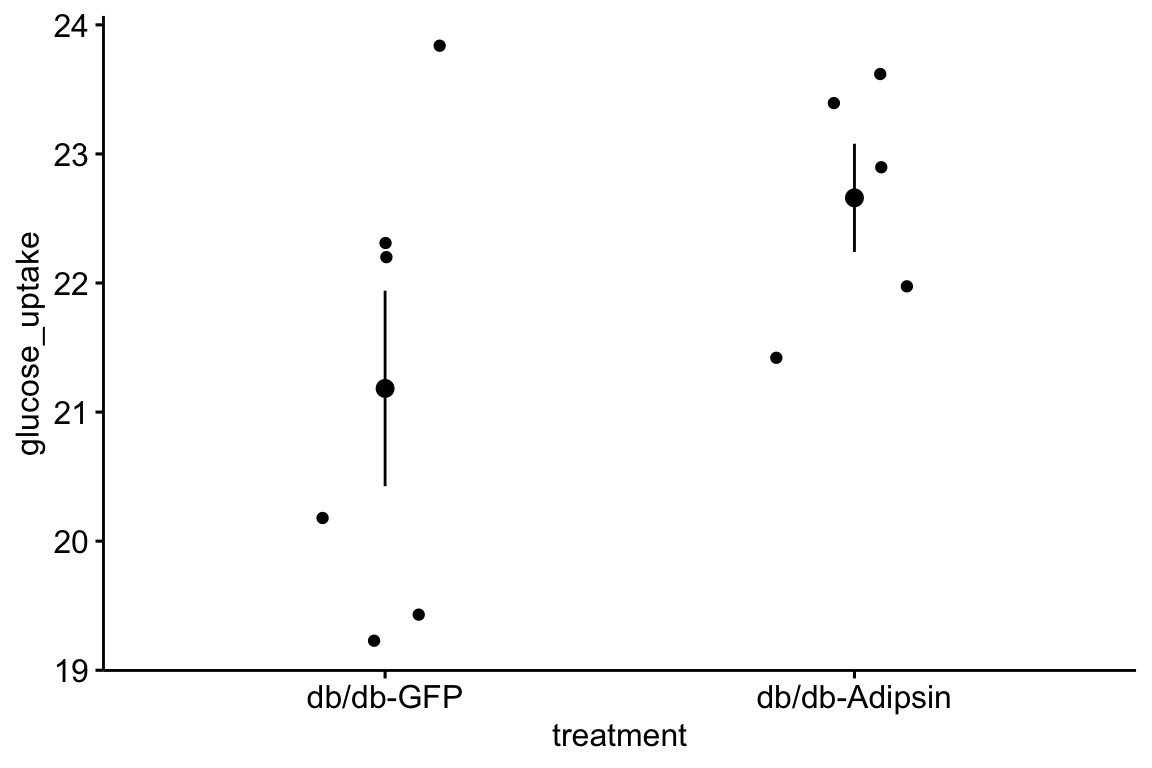
\includegraphics{Walker-elementary-statistical-modeling-draft_files/figure-latex/unnamed-chunk-16-1.pdf}
* no obvious unplausible outliers but two mice w/ high values in ``F/F HFD''
* similar at time zero (initial effect is trivial)

use AUC conditional on time 0 glucose

\begin{Shaded}
\begin{Highlighting}[]
\KeywordTok{qplot}\NormalTok{(}\DataTypeTok{x =}\NormalTok{ time,}
      \DataTypeTok{y =}\NormalTok{ glucose,}
      \DataTypeTok{data =}\NormalTok{ fig_2d,}
      \DataTypeTok{color =}\NormalTok{ treatment) }\OperatorTok{+}
\StringTok{  }\KeywordTok{geom_smooth}\NormalTok{()}
\end{Highlighting}
\end{Shaded}

\begin{verbatim}
## `geom_smooth()` using method = 'loess' and formula 'y ~ x'
\end{verbatim}

\begin{verbatim}
## Warning in grid.Call(C_textBounds, as.graphicsAnnot(x$label), x$x, x$y, :
## conversion failure on 'ASK1Δadipo chow' in 'mbcsToSbcs': dot substituted
## for <ce>
\end{verbatim}

\begin{verbatim}
## Warning in grid.Call(C_textBounds, as.graphicsAnnot(x$label), x$x, x$y, :
## conversion failure on 'ASK1Δadipo chow' in 'mbcsToSbcs': dot substituted
## for <94>
\end{verbatim}

\begin{verbatim}
## Warning in grid.Call(C_textBounds, as.graphicsAnnot(x$label), x$x, x$y, :
## conversion failure on 'ASK1Δadipo chow' in 'mbcsToSbcs': dot substituted
## for <ce>
\end{verbatim}

\begin{verbatim}
## Warning in grid.Call(C_textBounds, as.graphicsAnnot(x$label), x$x, x$y, :
## conversion failure on 'ASK1Δadipo chow' in 'mbcsToSbcs': dot substituted
## for <94>
\end{verbatim}

\begin{verbatim}
## Warning in grid.Call(C_textBounds, as.graphicsAnnot(x$label), x$x, x$y, :
## conversion failure on 'ASK1Δadipo chow' in 'mbcsToSbcs': dot substituted
## for <ce>
\end{verbatim}

\begin{verbatim}
## Warning in grid.Call(C_textBounds, as.graphicsAnnot(x$label), x$x, x$y, :
## conversion failure on 'ASK1Δadipo chow' in 'mbcsToSbcs': dot substituted
## for <94>
\end{verbatim}

\begin{verbatim}
## Warning in grid.Call(C_textBounds, as.graphicsAnnot(x$label), x$x, x$y, :
## conversion failure on 'ASK1Δadipo chow' in 'mbcsToSbcs': dot substituted
## for <ce>
\end{verbatim}

\begin{verbatim}
## Warning in grid.Call(C_textBounds, as.graphicsAnnot(x$label), x$x, x$y, :
## conversion failure on 'ASK1Δadipo chow' in 'mbcsToSbcs': dot substituted
## for <94>
\end{verbatim}

\begin{verbatim}
## Warning in grid.Call(C_textBounds, as.graphicsAnnot(x$label), x$x, x$y, :
## conversion failure on 'ASK1Δadipo chow' in 'mbcsToSbcs': dot substituted
## for <ce>
\end{verbatim}

\begin{verbatim}
## Warning in grid.Call(C_textBounds, as.graphicsAnnot(x$label), x$x, x$y, :
## conversion failure on 'ASK1Δadipo chow' in 'mbcsToSbcs': dot substituted
## for <94>
\end{verbatim}

\begin{verbatim}
## Warning in grid.Call(C_textBounds, as.graphicsAnnot(x$label), x$x, x$y, :
## conversion failure on 'ASK1Δadipo HFD' in 'mbcsToSbcs': dot substituted for
## <ce>
\end{verbatim}

\begin{verbatim}
## Warning in grid.Call(C_textBounds, as.graphicsAnnot(x$label), x$x, x$y, :
## conversion failure on 'ASK1Δadipo HFD' in 'mbcsToSbcs': dot substituted for
## <94>
\end{verbatim}

\begin{verbatim}
## Warning in grid.Call(C_textBounds, as.graphicsAnnot(x$label), x$x, x$y, :
## conversion failure on 'ASK1Δadipo HFD' in 'mbcsToSbcs': dot substituted for
## <ce>
\end{verbatim}

\begin{verbatim}
## Warning in grid.Call(C_textBounds, as.graphicsAnnot(x$label), x$x, x$y, :
## conversion failure on 'ASK1Δadipo HFD' in 'mbcsToSbcs': dot substituted for
## <94>
\end{verbatim}

\begin{verbatim}
## Warning in grid.Call(C_textBounds, as.graphicsAnnot(x$label), x$x, x$y, :
## conversion failure on 'ASK1Δadipo HFD' in 'mbcsToSbcs': dot substituted for
## <ce>
\end{verbatim}

\begin{verbatim}
## Warning in grid.Call(C_textBounds, as.graphicsAnnot(x$label), x$x, x$y, :
## conversion failure on 'ASK1Δadipo HFD' in 'mbcsToSbcs': dot substituted for
## <94>
\end{verbatim}

\begin{verbatim}
## Warning in grid.Call(C_textBounds, as.graphicsAnnot(x$label), x$x, x$y, :
## conversion failure on 'ASK1Δadipo HFD' in 'mbcsToSbcs': dot substituted for
## <ce>
\end{verbatim}

\begin{verbatim}
## Warning in grid.Call(C_textBounds, as.graphicsAnnot(x$label), x$x, x$y, :
## conversion failure on 'ASK1Δadipo HFD' in 'mbcsToSbcs': dot substituted for
## <94>
\end{verbatim}

\begin{verbatim}
## Warning in grid.Call(C_textBounds, as.graphicsAnnot(x$label), x$x, x$y, :
## conversion failure on 'ASK1Δadipo HFD' in 'mbcsToSbcs': dot substituted for
## <ce>
\end{verbatim}

\begin{verbatim}
## Warning in grid.Call(C_textBounds, as.graphicsAnnot(x$label), x$x, x$y, :
## conversion failure on 'ASK1Δadipo HFD' in 'mbcsToSbcs': dot substituted for
## <94>
\end{verbatim}

\begin{verbatim}
## Warning in grid.Call(C_textBounds, as.graphicsAnnot(x$label), x$x, x$y, :
## conversion failure on 'ASK1Δadipo chow' in 'mbcsToSbcs': dot substituted
## for <ce>
\end{verbatim}

\begin{verbatim}
## Warning in grid.Call(C_textBounds, as.graphicsAnnot(x$label), x$x, x$y, :
## conversion failure on 'ASK1Δadipo chow' in 'mbcsToSbcs': dot substituted
## for <94>
\end{verbatim}

\begin{verbatim}
## Warning in grid.Call(C_textBounds, as.graphicsAnnot(x$label), x$x, x$y, :
## conversion failure on 'ASK1Δadipo chow' in 'mbcsToSbcs': dot substituted
## for <ce>
\end{verbatim}

\begin{verbatim}
## Warning in grid.Call(C_textBounds, as.graphicsAnnot(x$label), x$x, x$y, :
## conversion failure on 'ASK1Δadipo chow' in 'mbcsToSbcs': dot substituted
## for <94>
\end{verbatim}

\begin{verbatim}
## Warning in grid.Call(C_textBounds, as.graphicsAnnot(x$label), x$x, x$y, :
## conversion failure on 'ASK1Δadipo chow' in 'mbcsToSbcs': dot substituted
## for <ce>
\end{verbatim}

\begin{verbatim}
## Warning in grid.Call(C_textBounds, as.graphicsAnnot(x$label), x$x, x$y, :
## conversion failure on 'ASK1Δadipo chow' in 'mbcsToSbcs': dot substituted
## for <94>
\end{verbatim}

\begin{verbatim}
## Warning in grid.Call(C_textBounds, as.graphicsAnnot(x$label), x$x, x$y, :
## conversion failure on 'ASK1Δadipo chow' in 'mbcsToSbcs': dot substituted
## for <ce>
\end{verbatim}

\begin{verbatim}
## Warning in grid.Call(C_textBounds, as.graphicsAnnot(x$label), x$x, x$y, :
## conversion failure on 'ASK1Δadipo chow' in 'mbcsToSbcs': dot substituted
## for <94>
\end{verbatim}

\begin{verbatim}
## Warning in grid.Call(C_textBounds, as.graphicsAnnot(x$label), x$x, x$y, :
## conversion failure on 'ASK1Δadipo chow' in 'mbcsToSbcs': dot substituted
## for <ce>
\end{verbatim}

\begin{verbatim}
## Warning in grid.Call(C_textBounds, as.graphicsAnnot(x$label), x$x, x$y, :
## conversion failure on 'ASK1Δadipo chow' in 'mbcsToSbcs': dot substituted
## for <94>
\end{verbatim}

\begin{verbatim}
## Warning in grid.Call(C_textBounds, as.graphicsAnnot(x$label), x$x, x$y, :
## conversion failure on 'ASK1Δadipo HFD' in 'mbcsToSbcs': dot substituted for
## <ce>
\end{verbatim}

\begin{verbatim}
## Warning in grid.Call(C_textBounds, as.graphicsAnnot(x$label), x$x, x$y, :
## conversion failure on 'ASK1Δadipo HFD' in 'mbcsToSbcs': dot substituted for
## <94>
\end{verbatim}

\begin{verbatim}
## Warning in grid.Call(C_textBounds, as.graphicsAnnot(x$label), x$x, x$y, :
## conversion failure on 'ASK1Δadipo HFD' in 'mbcsToSbcs': dot substituted for
## <ce>
\end{verbatim}

\begin{verbatim}
## Warning in grid.Call(C_textBounds, as.graphicsAnnot(x$label), x$x, x$y, :
## conversion failure on 'ASK1Δadipo HFD' in 'mbcsToSbcs': dot substituted for
## <94>
\end{verbatim}

\begin{verbatim}
## Warning in grid.Call(C_textBounds, as.graphicsAnnot(x$label), x$x, x$y, :
## conversion failure on 'ASK1Δadipo HFD' in 'mbcsToSbcs': dot substituted for
## <ce>
\end{verbatim}

\begin{verbatim}
## Warning in grid.Call(C_textBounds, as.graphicsAnnot(x$label), x$x, x$y, :
## conversion failure on 'ASK1Δadipo HFD' in 'mbcsToSbcs': dot substituted for
## <94>
\end{verbatim}

\begin{verbatim}
## Warning in grid.Call(C_textBounds, as.graphicsAnnot(x$label), x$x, x$y, :
## conversion failure on 'ASK1Δadipo HFD' in 'mbcsToSbcs': dot substituted for
## <ce>
\end{verbatim}

\begin{verbatim}
## Warning in grid.Call(C_textBounds, as.graphicsAnnot(x$label), x$x, x$y, :
## conversion failure on 'ASK1Δadipo HFD' in 'mbcsToSbcs': dot substituted for
## <94>
\end{verbatim}

\begin{verbatim}
## Warning in grid.Call(C_textBounds, as.graphicsAnnot(x$label), x$x, x$y, :
## conversion failure on 'ASK1Δadipo HFD' in 'mbcsToSbcs': dot substituted for
## <ce>
\end{verbatim}

\begin{verbatim}
## Warning in grid.Call(C_textBounds, as.graphicsAnnot(x$label), x$x, x$y, :
## conversion failure on 'ASK1Δadipo HFD' in 'mbcsToSbcs': dot substituted for
## <94>
\end{verbatim}

\begin{verbatim}
## Warning in grid.Call(C_textBounds, as.graphicsAnnot(x$label), x$x, x$y, :
## conversion failure on 'ASK1Δadipo chow' in 'mbcsToSbcs': dot substituted
## for <ce>
\end{verbatim}

\begin{verbatim}
## Warning in grid.Call(C_textBounds, as.graphicsAnnot(x$label), x$x, x$y, :
## conversion failure on 'ASK1Δadipo chow' in 'mbcsToSbcs': dot substituted
## for <94>
\end{verbatim}

\begin{verbatim}
## Warning in grid.Call(C_textBounds, as.graphicsAnnot(x$label), x$x, x$y, :
## conversion failure on 'ASK1Δadipo chow' in 'mbcsToSbcs': dot substituted
## for <ce>
\end{verbatim}

\begin{verbatim}
## Warning in grid.Call(C_textBounds, as.graphicsAnnot(x$label), x$x, x$y, :
## conversion failure on 'ASK1Δadipo chow' in 'mbcsToSbcs': dot substituted
## for <94>
\end{verbatim}

\begin{verbatim}
## Warning in grid.Call(C_textBounds, as.graphicsAnnot(x$label), x$x, x$y, :
## conversion failure on 'ASK1Δadipo chow' in 'mbcsToSbcs': dot substituted
## for <ce>
\end{verbatim}

\begin{verbatim}
## Warning in grid.Call(C_textBounds, as.graphicsAnnot(x$label), x$x, x$y, :
## conversion failure on 'ASK1Δadipo chow' in 'mbcsToSbcs': dot substituted
## for <94>
\end{verbatim}

\begin{verbatim}
## Warning in grid.Call(C_textBounds, as.graphicsAnnot(x$label), x$x, x$y, :
## conversion failure on 'ASK1Δadipo chow' in 'mbcsToSbcs': dot substituted
## for <ce>
\end{verbatim}

\begin{verbatim}
## Warning in grid.Call(C_textBounds, as.graphicsAnnot(x$label), x$x, x$y, :
## conversion failure on 'ASK1Δadipo chow' in 'mbcsToSbcs': dot substituted
## for <94>
\end{verbatim}

\begin{verbatim}
## Warning in grid.Call(C_textBounds, as.graphicsAnnot(x$label), x$x, x$y, :
## conversion failure on 'ASK1Δadipo chow' in 'mbcsToSbcs': dot substituted
## for <ce>
\end{verbatim}

\begin{verbatim}
## Warning in grid.Call(C_textBounds, as.graphicsAnnot(x$label), x$x, x$y, :
## conversion failure on 'ASK1Δadipo chow' in 'mbcsToSbcs': dot substituted
## for <94>
\end{verbatim}

\begin{verbatim}
## Warning in grid.Call(C_textBounds, as.graphicsAnnot(x$label), x$x, x$y, :
## conversion failure on 'ASK1Δadipo chow' in 'mbcsToSbcs': dot substituted
## for <ce>
\end{verbatim}

\begin{verbatim}
## Warning in grid.Call(C_textBounds, as.graphicsAnnot(x$label), x$x, x$y, :
## conversion failure on 'ASK1Δadipo chow' in 'mbcsToSbcs': dot substituted
## for <94>
\end{verbatim}

\begin{verbatim}
## Warning in grid.Call(C_textBounds, as.graphicsAnnot(x$label), x$x, x$y, :
## conversion failure on 'ASK1Δadipo chow' in 'mbcsToSbcs': dot substituted
## for <ce>
\end{verbatim}

\begin{verbatim}
## Warning in grid.Call(C_textBounds, as.graphicsAnnot(x$label), x$x, x$y, :
## conversion failure on 'ASK1Δadipo chow' in 'mbcsToSbcs': dot substituted
## for <94>
\end{verbatim}

\begin{verbatim}
## Warning in grid.Call(C_textBounds, as.graphicsAnnot(x$label), x$x, x$y, :
## conversion failure on 'ASK1Δadipo chow' in 'mbcsToSbcs': dot substituted
## for <ce>
\end{verbatim}

\begin{verbatim}
## Warning in grid.Call(C_textBounds, as.graphicsAnnot(x$label), x$x, x$y, :
## conversion failure on 'ASK1Δadipo chow' in 'mbcsToSbcs': dot substituted
## for <94>
\end{verbatim}

\begin{verbatim}
## Warning in grid.Call(C_textBounds, as.graphicsAnnot(x$label), x$x, x$y, :
## conversion failure on 'ASK1Δadipo chow' in 'mbcsToSbcs': dot substituted
## for <ce>
\end{verbatim}

\begin{verbatim}
## Warning in grid.Call(C_textBounds, as.graphicsAnnot(x$label), x$x, x$y, :
## conversion failure on 'ASK1Δadipo chow' in 'mbcsToSbcs': dot substituted
## for <94>
\end{verbatim}

\begin{verbatim}
## Warning in grid.Call(C_textBounds, as.graphicsAnnot(x$label), x$x, x$y, :
## conversion failure on 'ASK1Δadipo chow' in 'mbcsToSbcs': dot substituted
## for <ce>
\end{verbatim}

\begin{verbatim}
## Warning in grid.Call(C_textBounds, as.graphicsAnnot(x$label), x$x, x$y, :
## conversion failure on 'ASK1Δadipo chow' in 'mbcsToSbcs': dot substituted
## for <94>
\end{verbatim}

\begin{verbatim}
## Warning in grid.Call(C_textBounds, as.graphicsAnnot(x$label), x$x, x$y, :
## conversion failure on 'ASK1Δadipo chow' in 'mbcsToSbcs': dot substituted
## for <ce>
\end{verbatim}

\begin{verbatim}
## Warning in grid.Call(C_textBounds, as.graphicsAnnot(x$label), x$x, x$y, :
## conversion failure on 'ASK1Δadipo chow' in 'mbcsToSbcs': dot substituted
## for <94>
\end{verbatim}

\begin{verbatim}
## Warning in grid.Call(C_textBounds, as.graphicsAnnot(x$label), x$x, x$y, :
## conversion failure on 'ASK1Δadipo chow' in 'mbcsToSbcs': dot substituted
## for <ce>
\end{verbatim}

\begin{verbatim}
## Warning in grid.Call(C_textBounds, as.graphicsAnnot(x$label), x$x, x$y, :
## conversion failure on 'ASK1Δadipo chow' in 'mbcsToSbcs': dot substituted
## for <94>
\end{verbatim}

\begin{verbatim}
## Warning in grid.Call(C_textBounds, as.graphicsAnnot(x$label), x$x, x$y, :
## conversion failure on 'ASK1Δadipo chow' in 'mbcsToSbcs': dot substituted
## for <ce>
\end{verbatim}

\begin{verbatim}
## Warning in grid.Call(C_textBounds, as.graphicsAnnot(x$label), x$x, x$y, :
## conversion failure on 'ASK1Δadipo chow' in 'mbcsToSbcs': dot substituted
## for <94>
\end{verbatim}

\begin{verbatim}
## Warning in grid.Call(C_textBounds, as.graphicsAnnot(x$label), x$x, x$y, :
## conversion failure on 'ASK1Δadipo chow' in 'mbcsToSbcs': dot substituted
## for <ce>
\end{verbatim}

\begin{verbatim}
## Warning in grid.Call(C_textBounds, as.graphicsAnnot(x$label), x$x, x$y, :
## conversion failure on 'ASK1Δadipo chow' in 'mbcsToSbcs': dot substituted
## for <94>
\end{verbatim}

\begin{verbatim}
## Warning in grid.Call.graphics(C_text, as.graphicsAnnot(x$label), x$x,
## x$y, : conversion failure on 'ASK1Δadipo chow' in 'mbcsToSbcs': dot
## substituted for <ce>
\end{verbatim}

\begin{verbatim}
## Warning in grid.Call.graphics(C_text, as.graphicsAnnot(x$label), x$x,
## x$y, : conversion failure on 'ASK1Δadipo chow' in 'mbcsToSbcs': dot
## substituted for <94>
\end{verbatim}

\begin{verbatim}
## Warning in grid.Call(C_textBounds, as.graphicsAnnot(x$label), x$x, x$y, :
## conversion failure on 'ASK1Δadipo HFD' in 'mbcsToSbcs': dot substituted for
## <ce>
\end{verbatim}

\begin{verbatim}
## Warning in grid.Call(C_textBounds, as.graphicsAnnot(x$label), x$x, x$y, :
## conversion failure on 'ASK1Δadipo HFD' in 'mbcsToSbcs': dot substituted for
## <94>
\end{verbatim}

\begin{verbatim}
## Warning in grid.Call(C_textBounds, as.graphicsAnnot(x$label), x$x, x$y, :
## conversion failure on 'ASK1Δadipo HFD' in 'mbcsToSbcs': dot substituted for
## <ce>
\end{verbatim}

\begin{verbatim}
## Warning in grid.Call(C_textBounds, as.graphicsAnnot(x$label), x$x, x$y, :
## conversion failure on 'ASK1Δadipo HFD' in 'mbcsToSbcs': dot substituted for
## <94>
\end{verbatim}

\begin{verbatim}
## Warning in grid.Call(C_textBounds, as.graphicsAnnot(x$label), x$x, x$y, :
## conversion failure on 'ASK1Δadipo HFD' in 'mbcsToSbcs': dot substituted for
## <ce>
\end{verbatim}

\begin{verbatim}
## Warning in grid.Call(C_textBounds, as.graphicsAnnot(x$label), x$x, x$y, :
## conversion failure on 'ASK1Δadipo HFD' in 'mbcsToSbcs': dot substituted for
## <94>
\end{verbatim}

\begin{verbatim}
## Warning in grid.Call(C_textBounds, as.graphicsAnnot(x$label), x$x, x$y, :
## conversion failure on 'ASK1Δadipo HFD' in 'mbcsToSbcs': dot substituted for
## <ce>
\end{verbatim}

\begin{verbatim}
## Warning in grid.Call(C_textBounds, as.graphicsAnnot(x$label), x$x, x$y, :
## conversion failure on 'ASK1Δadipo HFD' in 'mbcsToSbcs': dot substituted for
## <94>
\end{verbatim}

\begin{verbatim}
## Warning in grid.Call(C_textBounds, as.graphicsAnnot(x$label), x$x, x$y, :
## conversion failure on 'ASK1Δadipo HFD' in 'mbcsToSbcs': dot substituted for
## <ce>
\end{verbatim}

\begin{verbatim}
## Warning in grid.Call(C_textBounds, as.graphicsAnnot(x$label), x$x, x$y, :
## conversion failure on 'ASK1Δadipo HFD' in 'mbcsToSbcs': dot substituted for
## <94>
\end{verbatim}

\begin{verbatim}
## Warning in grid.Call(C_textBounds, as.graphicsAnnot(x$label), x$x, x$y, :
## conversion failure on 'ASK1Δadipo HFD' in 'mbcsToSbcs': dot substituted for
## <ce>
\end{verbatim}

\begin{verbatim}
## Warning in grid.Call(C_textBounds, as.graphicsAnnot(x$label), x$x, x$y, :
## conversion failure on 'ASK1Δadipo HFD' in 'mbcsToSbcs': dot substituted for
## <94>
\end{verbatim}

\begin{verbatim}
## Warning in grid.Call(C_textBounds, as.graphicsAnnot(x$label), x$x, x$y, :
## conversion failure on 'ASK1Δadipo HFD' in 'mbcsToSbcs': dot substituted for
## <ce>
\end{verbatim}

\begin{verbatim}
## Warning in grid.Call(C_textBounds, as.graphicsAnnot(x$label), x$x, x$y, :
## conversion failure on 'ASK1Δadipo HFD' in 'mbcsToSbcs': dot substituted for
## <94>
\end{verbatim}

\begin{verbatim}
## Warning in grid.Call(C_textBounds, as.graphicsAnnot(x$label), x$x, x$y, :
## conversion failure on 'ASK1Δadipo HFD' in 'mbcsToSbcs': dot substituted for
## <ce>
\end{verbatim}

\begin{verbatim}
## Warning in grid.Call(C_textBounds, as.graphicsAnnot(x$label), x$x, x$y, :
## conversion failure on 'ASK1Δadipo HFD' in 'mbcsToSbcs': dot substituted for
## <94>
\end{verbatim}

\begin{verbatim}
## Warning in grid.Call(C_textBounds, as.graphicsAnnot(x$label), x$x, x$y, :
## conversion failure on 'ASK1Δadipo HFD' in 'mbcsToSbcs': dot substituted for
## <ce>
\end{verbatim}

\begin{verbatim}
## Warning in grid.Call(C_textBounds, as.graphicsAnnot(x$label), x$x, x$y, :
## conversion failure on 'ASK1Δadipo HFD' in 'mbcsToSbcs': dot substituted for
## <94>
\end{verbatim}

\begin{verbatim}
## Warning in grid.Call(C_textBounds, as.graphicsAnnot(x$label), x$x, x$y, :
## conversion failure on 'ASK1Δadipo HFD' in 'mbcsToSbcs': dot substituted for
## <ce>
\end{verbatim}

\begin{verbatim}
## Warning in grid.Call(C_textBounds, as.graphicsAnnot(x$label), x$x, x$y, :
## conversion failure on 'ASK1Δadipo HFD' in 'mbcsToSbcs': dot substituted for
## <94>
\end{verbatim}

\begin{verbatim}
## Warning in grid.Call(C_textBounds, as.graphicsAnnot(x$label), x$x, x$y, :
## conversion failure on 'ASK1Δadipo HFD' in 'mbcsToSbcs': dot substituted for
## <ce>
\end{verbatim}

\begin{verbatim}
## Warning in grid.Call(C_textBounds, as.graphicsAnnot(x$label), x$x, x$y, :
## conversion failure on 'ASK1Δadipo HFD' in 'mbcsToSbcs': dot substituted for
## <94>
\end{verbatim}

\begin{verbatim}
## Warning in grid.Call(C_textBounds, as.graphicsAnnot(x$label), x$x, x$y, :
## conversion failure on 'ASK1Δadipo HFD' in 'mbcsToSbcs': dot substituted for
## <ce>
\end{verbatim}

\begin{verbatim}
## Warning in grid.Call(C_textBounds, as.graphicsAnnot(x$label), x$x, x$y, :
## conversion failure on 'ASK1Δadipo HFD' in 'mbcsToSbcs': dot substituted for
## <94>
\end{verbatim}

\begin{verbatim}
## Warning in grid.Call(C_textBounds, as.graphicsAnnot(x$label), x$x, x$y, :
## conversion failure on 'ASK1Δadipo HFD' in 'mbcsToSbcs': dot substituted for
## <ce>
\end{verbatim}

\begin{verbatim}
## Warning in grid.Call(C_textBounds, as.graphicsAnnot(x$label), x$x, x$y, :
## conversion failure on 'ASK1Δadipo HFD' in 'mbcsToSbcs': dot substituted for
## <94>
\end{verbatim}

\begin{verbatim}
## Warning in grid.Call(C_textBounds, as.graphicsAnnot(x$label), x$x, x$y, :
## conversion failure on 'ASK1Δadipo HFD' in 'mbcsToSbcs': dot substituted for
## <ce>
\end{verbatim}

\begin{verbatim}
## Warning in grid.Call(C_textBounds, as.graphicsAnnot(x$label), x$x, x$y, :
## conversion failure on 'ASK1Δadipo HFD' in 'mbcsToSbcs': dot substituted for
## <94>
\end{verbatim}

\begin{verbatim}
## Warning in grid.Call.graphics(C_text, as.graphicsAnnot(x$label), x$x,
## x$y, : conversion failure on 'ASK1Δadipo HFD' in 'mbcsToSbcs': dot
## substituted for <ce>
\end{verbatim}

\begin{verbatim}
## Warning in grid.Call.graphics(C_text, as.graphicsAnnot(x$label), x$x,
## x$y, : conversion failure on 'ASK1Δadipo HFD' in 'mbcsToSbcs': dot
## substituted for <94>
\end{verbatim}

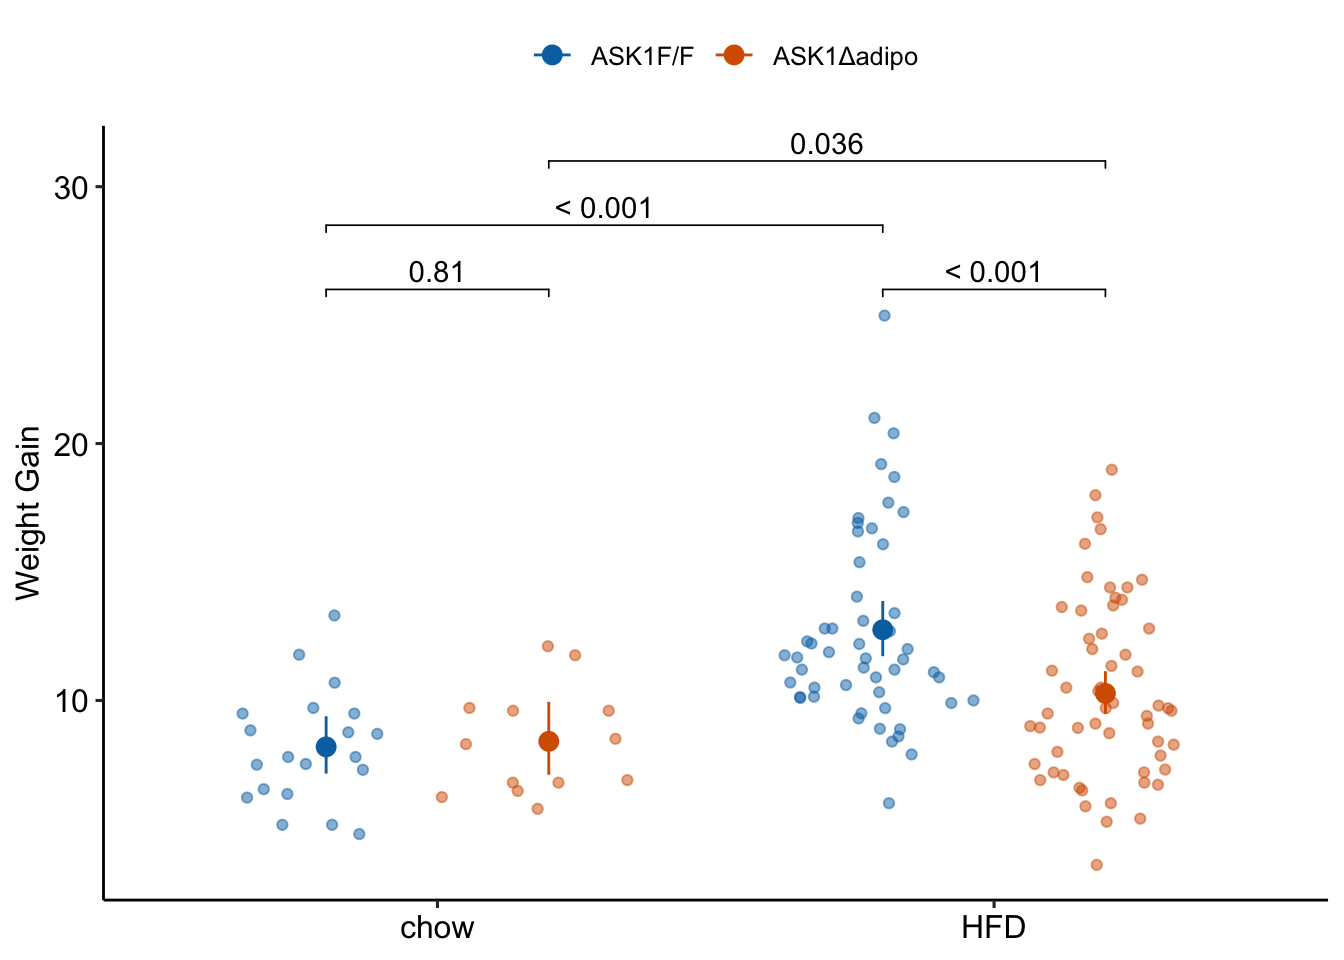
\includegraphics{Walker-elementary-statistical-modeling-draft_files/figure-latex/unnamed-chunk-17-1.pdf}

\hypertarget{figure-2d-fit-the-model}{%
\subsection{Figure 2d -- fit the model}\label{figure-2d-fit-the-model}}

\hypertarget{figure-2d-check-the-model}{%
\subsection{Figure 2d -- check the model}\label{figure-2d-check-the-model}}

\hypertarget{figure-2d-inference}{%
\subsection{Figure 2d -- inference}\label{figure-2d-inference}}

\hypertarget{figure-2d-plot-the-model}{%
\subsection{Figure 2d -- plot the model}\label{figure-2d-plot-the-model}}

\hypertarget{figure-2e-effect-of-ask1-ko-on-glucose-tolerance-summary-measure}{%
\section{Figure 2e -- Effect of ASK1 KO on glucose tolerance (summary measure)}\label{figure-2e-effect-of-ask1-ko-on-glucose-tolerance-summary-measure}}

The researchers did create a table to import but this analysis uses the mean post-baseline glucose amount as the response instead of the area under the curve of over the full 120 minutes. This mean is computed as the post-baseline area under the curve divided by the duration of time of the post-baseline measures (105 minutes). This analysis will use fig\_2d\_wide since there is only one a single Y variable per mouse.

\hypertarget{figure-2e-message-the-data}{%
\subsection{Figure 2e -- message the data}\label{figure-2e-message-the-data}}

\begin{Shaded}
\begin{Highlighting}[]
\CommentTok{# AUC of post-baseline values}
\CommentTok{# do this after melt as we don't need this in long format)}
\NormalTok{fig_2d_wide[, glucose_}\DecValTok{0} \OperatorTok{:}\ErrorTok{=}\StringTok{ }\KeywordTok{get}\NormalTok{(}\StringTok{"0"}\NormalTok{)]}

\NormalTok{times <-}\StringTok{ }\KeywordTok{c}\NormalTok{(}\DecValTok{0}\NormalTok{, }\DecValTok{15}\NormalTok{, }\DecValTok{30}\NormalTok{, }\DecValTok{45}\NormalTok{, }\DecValTok{60}\NormalTok{, }\DecValTok{90}\NormalTok{, }\DecValTok{120}\NormalTok{)}
\NormalTok{time_cols <-}\StringTok{ }\KeywordTok{as.character}\NormalTok{(times)}
\NormalTok{Y <-}\StringTok{ }\NormalTok{fig_2d_wide[, .SD, .SDcols =}\StringTok{ }\NormalTok{time_cols]}
\NormalTok{fig_2d_wide[, glucose_mean }\OperatorTok{:}\ErrorTok{=}\StringTok{ }\KeywordTok{apply}\NormalTok{(Y, }\DecValTok{1}\NormalTok{, auc,}
                           \DataTypeTok{x=}\NormalTok{times,}
                           \DataTypeTok{method =} \StringTok{"post_0_auc"}\NormalTok{,}
                           \DataTypeTok{average =} \OtherTok{TRUE}\NormalTok{)]}
\end{Highlighting}
\end{Shaded}

\hypertarget{figure-2e-exploratory-plots}{%
\subsection{Figure 2e -- exploratory plots}\label{figure-2e-exploratory-plots}}

\begin{Shaded}
\begin{Highlighting}[]
\KeywordTok{qplot}\NormalTok{(}\DataTypeTok{x =}\NormalTok{ treatment, }\DataTypeTok{y =}\NormalTok{ glucose_mean, }\DataTypeTok{data =}\NormalTok{ fig_2d_wide)}
\end{Highlighting}
\end{Shaded}

\begin{verbatim}
## Warning in grid.Call(C_textBounds, as.graphicsAnnot(x$label), x$x, x$y, :
## conversion failure on 'ASK1Δadipo chow' in 'mbcsToSbcs': dot substituted
## for <ce>
\end{verbatim}

\begin{verbatim}
## Warning in grid.Call(C_textBounds, as.graphicsAnnot(x$label), x$x, x$y, :
## conversion failure on 'ASK1Δadipo chow' in 'mbcsToSbcs': dot substituted
## for <94>
\end{verbatim}

\begin{verbatim}
## Warning in grid.Call(C_textBounds, as.graphicsAnnot(x$label), x$x, x$y, :
## conversion failure on 'ASK1Δadipo HFD' in 'mbcsToSbcs': dot substituted for
## <ce>
\end{verbatim}

\begin{verbatim}
## Warning in grid.Call(C_textBounds, as.graphicsAnnot(x$label), x$x, x$y, :
## conversion failure on 'ASK1Δadipo HFD' in 'mbcsToSbcs': dot substituted for
## <94>
\end{verbatim}

\begin{verbatim}
## Warning in grid.Call(C_textBounds, as.graphicsAnnot(x$label), x$x, x$y, :
## conversion failure on 'ASK1Δadipo chow' in 'mbcsToSbcs': dot substituted
## for <ce>
\end{verbatim}

\begin{verbatim}
## Warning in grid.Call(C_textBounds, as.graphicsAnnot(x$label), x$x, x$y, :
## conversion failure on 'ASK1Δadipo chow' in 'mbcsToSbcs': dot substituted
## for <94>
\end{verbatim}

\begin{verbatim}
## Warning in grid.Call(C_textBounds, as.graphicsAnnot(x$label), x$x, x$y, :
## conversion failure on 'ASK1Δadipo HFD' in 'mbcsToSbcs': dot substituted for
## <ce>
\end{verbatim}

\begin{verbatim}
## Warning in grid.Call(C_textBounds, as.graphicsAnnot(x$label), x$x, x$y, :
## conversion failure on 'ASK1Δadipo HFD' in 'mbcsToSbcs': dot substituted for
## <94>
\end{verbatim}

\begin{verbatim}
## Warning in grid.Call(C_textBounds, as.graphicsAnnot(x$label), x$x, x$y, :
## conversion failure on 'ASK1Δadipo chow' in 'mbcsToSbcs': dot substituted
## for <ce>
\end{verbatim}

\begin{verbatim}
## Warning in grid.Call(C_textBounds, as.graphicsAnnot(x$label), x$x, x$y, :
## conversion failure on 'ASK1Δadipo chow' in 'mbcsToSbcs': dot substituted
## for <94>
\end{verbatim}

\begin{verbatim}
## Warning in grid.Call(C_textBounds, as.graphicsAnnot(x$label), x$x, x$y, :
## conversion failure on 'ASK1Δadipo HFD' in 'mbcsToSbcs': dot substituted for
## <ce>
\end{verbatim}

\begin{verbatim}
## Warning in grid.Call(C_textBounds, as.graphicsAnnot(x$label), x$x, x$y, :
## conversion failure on 'ASK1Δadipo HFD' in 'mbcsToSbcs': dot substituted for
## <94>
\end{verbatim}

\begin{verbatim}
## Warning in grid.Call(C_textBounds, as.graphicsAnnot(x$label), x$x, x$y, :
## conversion failure on 'ASK1Δadipo chow' in 'mbcsToSbcs': dot substituted
## for <ce>
\end{verbatim}

\begin{verbatim}
## Warning in grid.Call(C_textBounds, as.graphicsAnnot(x$label), x$x, x$y, :
## conversion failure on 'ASK1Δadipo chow' in 'mbcsToSbcs': dot substituted
## for <94>
\end{verbatim}

\begin{verbatim}
## Warning in grid.Call(C_textBounds, as.graphicsAnnot(x$label), x$x, x$y, :
## conversion failure on 'ASK1Δadipo HFD' in 'mbcsToSbcs': dot substituted for
## <ce>
\end{verbatim}

\begin{verbatim}
## Warning in grid.Call(C_textBounds, as.graphicsAnnot(x$label), x$x, x$y, :
## conversion failure on 'ASK1Δadipo HFD' in 'mbcsToSbcs': dot substituted for
## <94>
\end{verbatim}

\begin{verbatim}
## Warning in grid.Call(C_textBounds, as.graphicsAnnot(x$label), x$x, x$y, :
## conversion failure on 'ASK1Δadipo chow' in 'mbcsToSbcs': dot substituted
## for <ce>
\end{verbatim}

\begin{verbatim}
## Warning in grid.Call(C_textBounds, as.graphicsAnnot(x$label), x$x, x$y, :
## conversion failure on 'ASK1Δadipo chow' in 'mbcsToSbcs': dot substituted
## for <94>
\end{verbatim}

\begin{verbatim}
## Warning in grid.Call(C_textBounds, as.graphicsAnnot(x$label), x$x, x$y, :
## conversion failure on 'ASK1Δadipo HFD' in 'mbcsToSbcs': dot substituted for
## <ce>
\end{verbatim}

\begin{verbatim}
## Warning in grid.Call(C_textBounds, as.graphicsAnnot(x$label), x$x, x$y, :
## conversion failure on 'ASK1Δadipo HFD' in 'mbcsToSbcs': dot substituted for
## <94>
\end{verbatim}

\begin{verbatim}
## Warning in grid.Call(C_textBounds, as.graphicsAnnot(x$label), x$x, x$y, :
## conversion failure on 'ASK1Δadipo chow' in 'mbcsToSbcs': dot substituted
## for <ce>
\end{verbatim}

\begin{verbatim}
## Warning in grid.Call(C_textBounds, as.graphicsAnnot(x$label), x$x, x$y, :
## conversion failure on 'ASK1Δadipo chow' in 'mbcsToSbcs': dot substituted
## for <94>
\end{verbatim}

\begin{verbatim}
## Warning in grid.Call(C_textBounds, as.graphicsAnnot(x$label), x$x, x$y, :
## conversion failure on 'ASK1Δadipo HFD' in 'mbcsToSbcs': dot substituted for
## <ce>
\end{verbatim}

\begin{verbatim}
## Warning in grid.Call(C_textBounds, as.graphicsAnnot(x$label), x$x, x$y, :
## conversion failure on 'ASK1Δadipo HFD' in 'mbcsToSbcs': dot substituted for
## <94>
\end{verbatim}

\begin{verbatim}
## Warning in grid.Call(C_textBounds, as.graphicsAnnot(x$label), x$x, x$y, :
## conversion failure on 'ASK1Δadipo chow' in 'mbcsToSbcs': dot substituted
## for <ce>
\end{verbatim}

\begin{verbatim}
## Warning in grid.Call(C_textBounds, as.graphicsAnnot(x$label), x$x, x$y, :
## conversion failure on 'ASK1Δadipo chow' in 'mbcsToSbcs': dot substituted
## for <94>
\end{verbatim}

\begin{verbatim}
## Warning in grid.Call(C_textBounds, as.graphicsAnnot(x$label), x$x, x$y, :
## conversion failure on 'ASK1Δadipo HFD' in 'mbcsToSbcs': dot substituted for
## <ce>
\end{verbatim}

\begin{verbatim}
## Warning in grid.Call(C_textBounds, as.graphicsAnnot(x$label), x$x, x$y, :
## conversion failure on 'ASK1Δadipo HFD' in 'mbcsToSbcs': dot substituted for
## <94>
\end{verbatim}

\begin{verbatim}
## Warning in grid.Call(C_textBounds, as.graphicsAnnot(x$label), x$x, x$y, :
## conversion failure on 'ASK1Δadipo chow' in 'mbcsToSbcs': dot substituted
## for <ce>
\end{verbatim}

\begin{verbatim}
## Warning in grid.Call(C_textBounds, as.graphicsAnnot(x$label), x$x, x$y, :
## conversion failure on 'ASK1Δadipo chow' in 'mbcsToSbcs': dot substituted
## for <94>
\end{verbatim}

\begin{verbatim}
## Warning in grid.Call(C_textBounds, as.graphicsAnnot(x$label), x$x, x$y, :
## conversion failure on 'ASK1Δadipo HFD' in 'mbcsToSbcs': dot substituted for
## <ce>
\end{verbatim}

\begin{verbatim}
## Warning in grid.Call(C_textBounds, as.graphicsAnnot(x$label), x$x, x$y, :
## conversion failure on 'ASK1Δadipo HFD' in 'mbcsToSbcs': dot substituted for
## <94>
\end{verbatim}

\begin{verbatim}
## Warning in grid.Call(C_textBounds, as.graphicsAnnot(x$label), x$x, x$y, :
## conversion failure on 'ASK1Δadipo chow' in 'mbcsToSbcs': dot substituted
## for <ce>
\end{verbatim}

\begin{verbatim}
## Warning in grid.Call(C_textBounds, as.graphicsAnnot(x$label), x$x, x$y, :
## conversion failure on 'ASK1Δadipo chow' in 'mbcsToSbcs': dot substituted
## for <94>
\end{verbatim}

\begin{verbatim}
## Warning in grid.Call(C_textBounds, as.graphicsAnnot(x$label), x$x, x$y, :
## conversion failure on 'ASK1Δadipo HFD' in 'mbcsToSbcs': dot substituted for
## <ce>
\end{verbatim}

\begin{verbatim}
## Warning in grid.Call(C_textBounds, as.graphicsAnnot(x$label), x$x, x$y, :
## conversion failure on 'ASK1Δadipo HFD' in 'mbcsToSbcs': dot substituted for
## <94>
\end{verbatim}

\begin{verbatim}
## Warning in grid.Call(C_textBounds, as.graphicsAnnot(x$label), x$x, x$y, :
## conversion failure on 'ASK1Δadipo chow' in 'mbcsToSbcs': dot substituted
## for <ce>
\end{verbatim}

\begin{verbatim}
## Warning in grid.Call(C_textBounds, as.graphicsAnnot(x$label), x$x, x$y, :
## conversion failure on 'ASK1Δadipo chow' in 'mbcsToSbcs': dot substituted
## for <94>
\end{verbatim}

\begin{verbatim}
## Warning in grid.Call(C_textBounds, as.graphicsAnnot(x$label), x$x, x$y, :
## conversion failure on 'ASK1Δadipo HFD' in 'mbcsToSbcs': dot substituted for
## <ce>
\end{verbatim}

\begin{verbatim}
## Warning in grid.Call(C_textBounds, as.graphicsAnnot(x$label), x$x, x$y, :
## conversion failure on 'ASK1Δadipo HFD' in 'mbcsToSbcs': dot substituted for
## <94>
\end{verbatim}

\begin{verbatim}
## Warning in grid.Call(C_textBounds, as.graphicsAnnot(x$label), x$x, x$y, :
## conversion failure on 'ASK1Δadipo chow' in 'mbcsToSbcs': dot substituted
## for <ce>
\end{verbatim}

\begin{verbatim}
## Warning in grid.Call(C_textBounds, as.graphicsAnnot(x$label), x$x, x$y, :
## conversion failure on 'ASK1Δadipo chow' in 'mbcsToSbcs': dot substituted
## for <94>
\end{verbatim}

\begin{verbatim}
## Warning in grid.Call(C_textBounds, as.graphicsAnnot(x$label), x$x, x$y, :
## conversion failure on 'ASK1Δadipo HFD' in 'mbcsToSbcs': dot substituted for
## <ce>
\end{verbatim}

\begin{verbatim}
## Warning in grid.Call(C_textBounds, as.graphicsAnnot(x$label), x$x, x$y, :
## conversion failure on 'ASK1Δadipo HFD' in 'mbcsToSbcs': dot substituted for
## <94>
\end{verbatim}

\begin{verbatim}
## Warning in grid.Call(C_textBounds, as.graphicsAnnot(x$label), x$x, x$y, :
## conversion failure on 'ASK1Δadipo chow' in 'mbcsToSbcs': dot substituted
## for <ce>
\end{verbatim}

\begin{verbatim}
## Warning in grid.Call(C_textBounds, as.graphicsAnnot(x$label), x$x, x$y, :
## conversion failure on 'ASK1Δadipo chow' in 'mbcsToSbcs': dot substituted
## for <94>
\end{verbatim}

\begin{verbatim}
## Warning in grid.Call(C_textBounds, as.graphicsAnnot(x$label), x$x, x$y, :
## conversion failure on 'ASK1Δadipo HFD' in 'mbcsToSbcs': dot substituted for
## <ce>
\end{verbatim}

\begin{verbatim}
## Warning in grid.Call(C_textBounds, as.graphicsAnnot(x$label), x$x, x$y, :
## conversion failure on 'ASK1Δadipo HFD' in 'mbcsToSbcs': dot substituted for
## <94>
\end{verbatim}

\begin{verbatim}
## Warning in grid.Call(C_textBounds, as.graphicsAnnot(x$label), x$x, x$y, :
## conversion failure on 'ASK1Δadipo chow' in 'mbcsToSbcs': dot substituted
## for <ce>
\end{verbatim}

\begin{verbatim}
## Warning in grid.Call(C_textBounds, as.graphicsAnnot(x$label), x$x, x$y, :
## conversion failure on 'ASK1Δadipo chow' in 'mbcsToSbcs': dot substituted
## for <94>
\end{verbatim}

\begin{verbatim}
## Warning in grid.Call(C_textBounds, as.graphicsAnnot(x$label), x$x, x$y, :
## conversion failure on 'ASK1Δadipo HFD' in 'mbcsToSbcs': dot substituted for
## <ce>
\end{verbatim}

\begin{verbatim}
## Warning in grid.Call(C_textBounds, as.graphicsAnnot(x$label), x$x, x$y, :
## conversion failure on 'ASK1Δadipo HFD' in 'mbcsToSbcs': dot substituted for
## <94>
\end{verbatim}

\begin{verbatim}
## Warning in grid.Call.graphics(C_text, as.graphicsAnnot(x$label), x$x,
## x$y, : conversion failure on 'ASK1Δadipo chow' in 'mbcsToSbcs': dot
## substituted for <ce>
\end{verbatim}

\begin{verbatim}
## Warning in grid.Call.graphics(C_text, as.graphicsAnnot(x$label), x$x,
## x$y, : conversion failure on 'ASK1Δadipo chow' in 'mbcsToSbcs': dot
## substituted for <94>
\end{verbatim}

\begin{verbatim}
## Warning in grid.Call.graphics(C_text, as.graphicsAnnot(x$label), x$x,
## x$y, : conversion failure on 'ASK1Δadipo HFD' in 'mbcsToSbcs': dot
## substituted for <ce>
\end{verbatim}

\begin{verbatim}
## Warning in grid.Call.graphics(C_text, as.graphicsAnnot(x$label), x$x,
## x$y, : conversion failure on 'ASK1Δadipo HFD' in 'mbcsToSbcs': dot
## substituted for <94>
\end{verbatim}

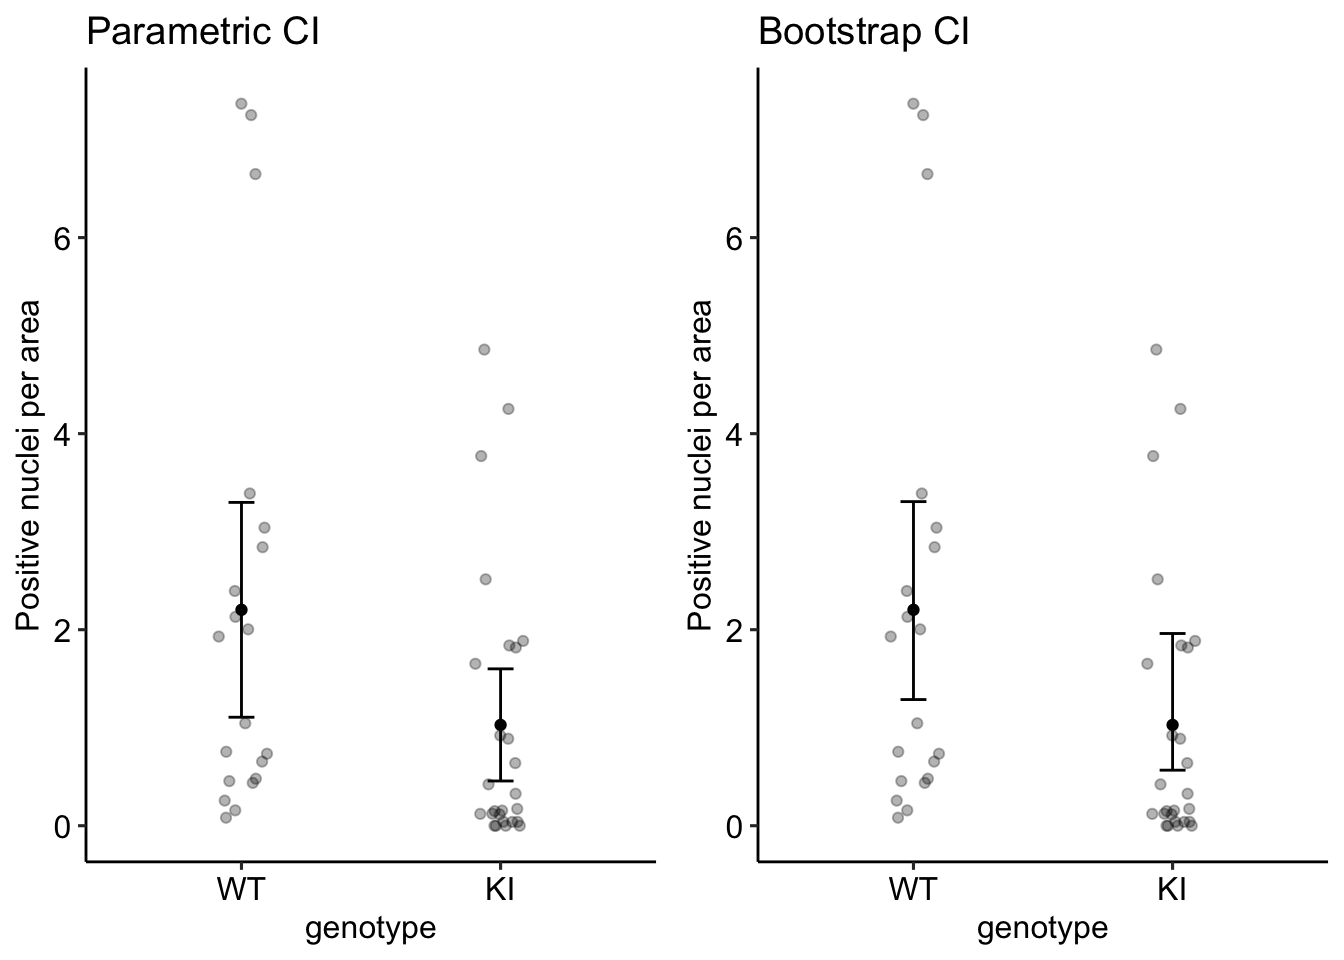
\includegraphics{Walker-elementary-statistical-modeling-draft_files/figure-latex/unnamed-chunk-19-1.pdf}

\hypertarget{figure-2e-fit-the-model}{%
\subsection{Figure 2e -- fit the model}\label{figure-2e-fit-the-model}}

\begin{Shaded}
\begin{Highlighting}[]
\NormalTok{fig_2e_m1 <-}\StringTok{ }\KeywordTok{lm}\NormalTok{(glucose_mean }\OperatorTok{~}\StringTok{ }\NormalTok{glucose_}\DecValTok{0} \OperatorTok{+}\StringTok{ }\NormalTok{ask1}\OperatorTok{*}\NormalTok{diet, }\DataTypeTok{data =}\NormalTok{ fig_2d_wide)}
\end{Highlighting}
\end{Shaded}

\hypertarget{figure-2e-check-the-model}{%
\subsection{Figure 2e -- check the model}\label{figure-2e-check-the-model}}

\begin{Shaded}
\begin{Highlighting}[]
\CommentTok{# check normality assumption}
\KeywordTok{set.seed}\NormalTok{(}\DecValTok{1}\NormalTok{)}
\KeywordTok{qqPlot}\NormalTok{(fig_2e_m1, }\DataTypeTok{id=}\OtherTok{FALSE}\NormalTok{)}
\end{Highlighting}
\end{Shaded}

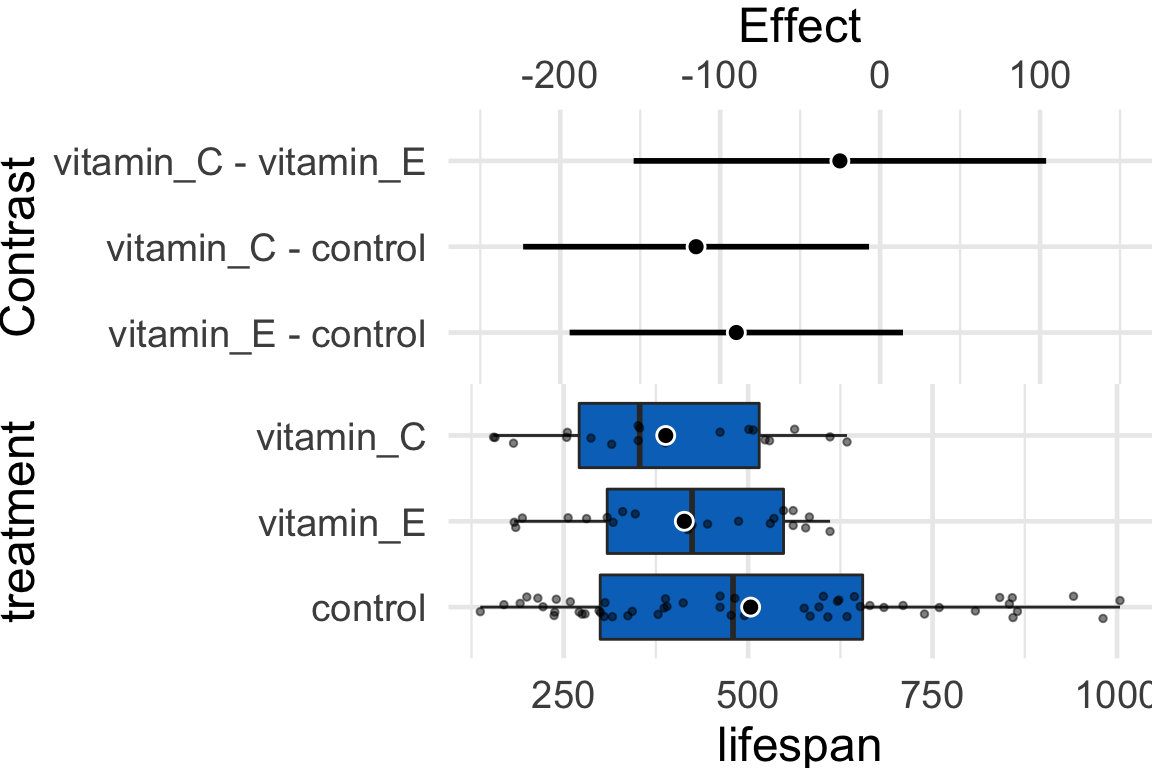
\includegraphics{Walker-elementary-statistical-modeling-draft_files/figure-latex/unnamed-chunk-21-1.pdf}

\begin{Shaded}
\begin{Highlighting}[]
\KeywordTok{spreadLevelPlot}\NormalTok{(fig_2e_m1, }\DataTypeTok{id=}\OtherTok{FALSE}\NormalTok{)}
\end{Highlighting}
\end{Shaded}

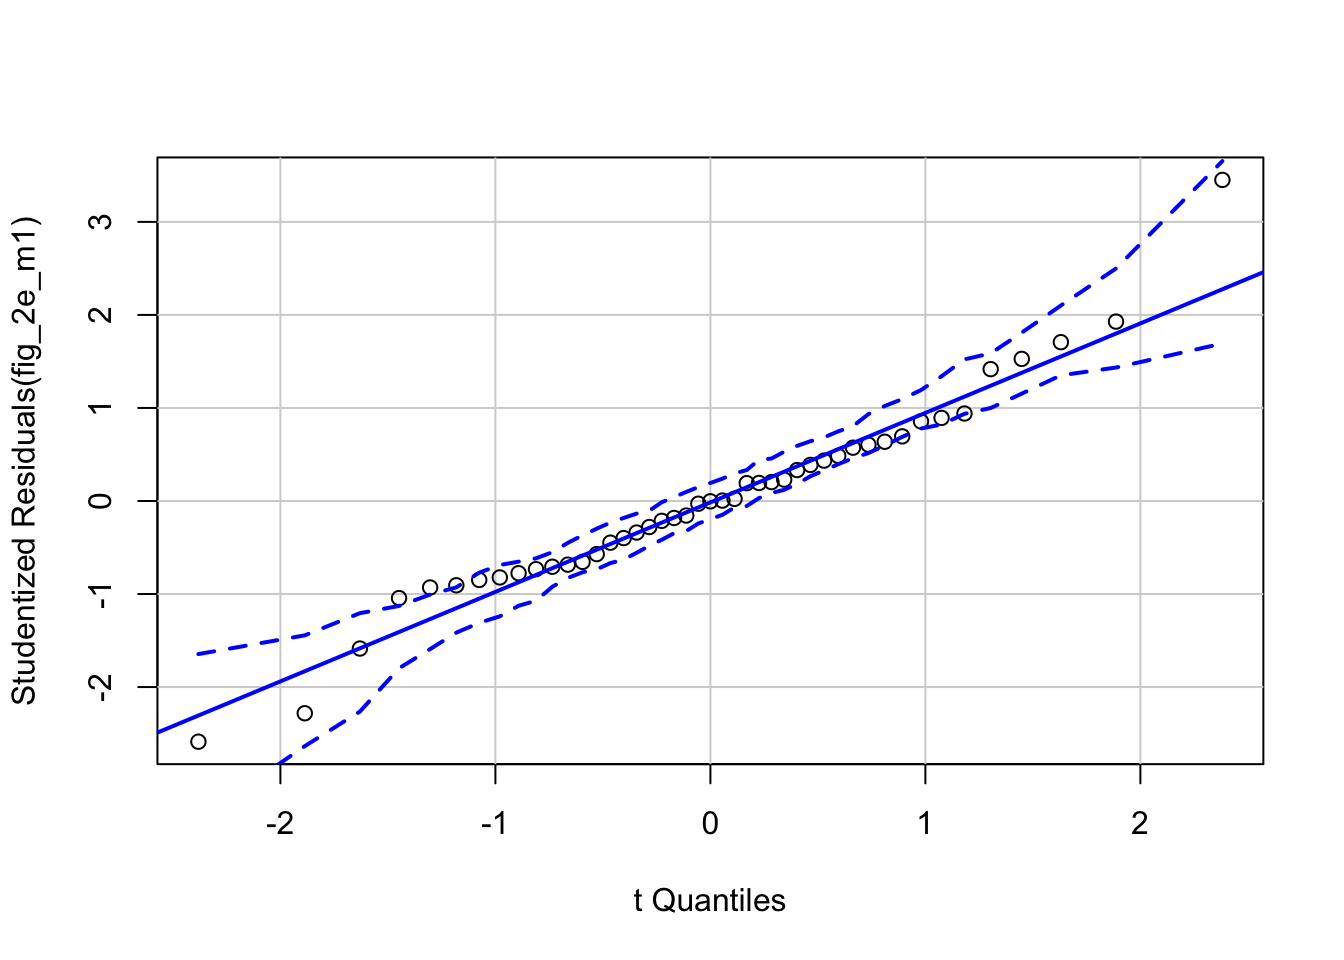
\includegraphics{Walker-elementary-statistical-modeling-draft_files/figure-latex/unnamed-chunk-22-1.pdf}

\begin{verbatim}
## 
## Suggested power transformation:  -0.4035073
\end{verbatim}

\hypertarget{figure-2e-inference-from-the-model}{%
\subsection{Figure 2e -- inference from the model}\label{figure-2e-inference-from-the-model}}

\begin{Shaded}
\begin{Highlighting}[]
\NormalTok{fig_2e_m1_coef <-}\StringTok{ }\KeywordTok{coef}\NormalTok{(}\KeywordTok{summary}\NormalTok{(fig_2e_m1))}
\NormalTok{fig_2e_m1_coef}
\end{Highlighting}
\end{Shaded}

\begin{verbatim}
##                          Estimate Std. Error    t value     Pr(>|t|)
## (Intercept)             8.6835026  1.2556730  6.9154169 2.460045e-08
## glucose_0               1.2194720  0.2390919  5.1004329 8.592596e-06
## ask1ASK1Δadipo         -0.3488511  0.8759124 -0.3982716 6.925479e-01
## dietHFD                 4.2782121  0.7908612  5.4095613 3.185930e-06
## ask1ASK1Δadipo:dietHFD -2.7503448  1.1288320 -2.4364518 1.937783e-02
\end{verbatim}

\begin{Shaded}
\begin{Highlighting}[]
\NormalTok{fig_2e_m1_emm <-}\StringTok{ }\KeywordTok{emmeans}\NormalTok{(fig_2e_m1, }\DataTypeTok{specs =} \KeywordTok{c}\NormalTok{(}\StringTok{"diet"}\NormalTok{, }\StringTok{"ask1"}\NormalTok{))}
\NormalTok{fig_2e_m1_pairs <-}\StringTok{ }\KeywordTok{contrast}\NormalTok{(fig_2e_m1_emm,}
                     \DataTypeTok{method =} \StringTok{"revpairwise"}\NormalTok{,}
                     \DataTypeTok{simple =} \StringTok{"each"}\NormalTok{,}
                     \DataTypeTok{combine =} \OtherTok{TRUE}\NormalTok{,}
                     \DataTypeTok{adjust =} \StringTok{"none"}\NormalTok{) }\OperatorTok
\StringTok{  }\KeywordTok{summary}\NormalTok{(}\DataTypeTok{infer =} \OtherTok{TRUE}\NormalTok{)}
\end{Highlighting}
\end{Shaded}

\begin{Shaded}
\begin{Highlighting}[]
\NormalTok{fig_2e_m1_emm}
\end{Highlighting}
\end{Shaded}

\begin{verbatim}
##  diet ask1       emmean    SE df lower.CL upper.CL
##  chow ASK1F/F      14.7 0.587 40     13.5     15.9
##  HFD  ASK1F/F      18.9 0.520 40     17.9     20.0
##  chow ASK1Δadipo   14.3 0.659 40     13.0     15.7
##  HFD  ASK1Δadipo   15.9 0.493 40     14.9     16.8
## 
## Confidence level used: 0.95
\end{verbatim}

\begin{Shaded}
\begin{Highlighting}[]
\NormalTok{fig_2e_m1_pairs}
\end{Highlighting}
\end{Shaded}

\begin{verbatim}
##  ask1       diet contrast             estimate    SE df lower.CL upper.CL
##  ASK1F/F    .    HFD - chow              4.278 0.791 40    2.680     5.88
##  ASK1Δadipo .    HFD - chow              1.528 0.824 40   -0.138     3.19
##  .          chow ASK1Δadipo - ASK1F/F   -0.349 0.876 40   -2.119     1.42
##  .          HFD  ASK1Δadipo - ASK1F/F   -3.099 0.715 40   -4.544    -1.65
##  t.ratio p.value
##   5.410  <.0001 
##   1.853  0.0712 
##  -0.398  0.6925 
##  -4.335  0.0001 
## 
## Confidence level used: 0.95
\end{verbatim}

\hypertarget{figure-2e-plot-the-model}{%
\subsection{Figure 2e -- plot the model}\label{figure-2e-plot-the-model}}

\begin{Shaded}
\begin{Highlighting}[]
\NormalTok{fig_2e_gg <-}\StringTok{ }\KeywordTok{gg_mean_error}\NormalTok{(}\DataTypeTok{data =}\NormalTok{ fig_2d_wide,}
                          \DataTypeTok{fit =}\NormalTok{ fig_2e_m1,}
                          \DataTypeTok{fit_emm =}\NormalTok{ fig_2e_m1_emm,}
                          \DataTypeTok{fit_pairs =}\NormalTok{ fig_2e_m1_pairs,}
                          \DataTypeTok{x_col =} \StringTok{"diet"}\NormalTok{,}
                          \DataTypeTok{y_col =} \StringTok{"glucose_mean"}\NormalTok{,}
                          \DataTypeTok{g_col =} \StringTok{"ask1"}\NormalTok{,}
                          \DataTypeTok{wrap_col =} \OtherTok{NULL}\NormalTok{,}
                          \DataTypeTok{x_label =} \StringTok{"none"}\NormalTok{,}
                          \DataTypeTok{y_label =} \StringTok{"Post-baseline glucose (mmol per l)"}\NormalTok{,}
                          \DataTypeTok{g_label =} \StringTok{""}\NormalTok{,}
                          \DataTypeTok{dots =} \StringTok{"sina"}\NormalTok{,}
                          \DataTypeTok{dodge_width =} \FloatTok{0.8}\NormalTok{,}
                          \DataTypeTok{adjust =} \FloatTok{0.5}\NormalTok{,}
                          \DataTypeTok{p_show =} \KeywordTok{c}\NormalTok{(}\DecValTok{3}\NormalTok{, }\DecValTok{4}\NormalTok{, }\DecValTok{2}\NormalTok{,}\DecValTok{1}\NormalTok{),}
                          \DataTypeTok{p_pos =} \KeywordTok{c}\NormalTok{(}\DecValTok{1}\NormalTok{,}\DecValTok{1}\NormalTok{,}\DecValTok{2}\NormalTok{,}\DecValTok{3}\NormalTok{))}
\NormalTok{fig_2e_gg}
\end{Highlighting}
\end{Shaded}

\begin{verbatim}
## Warning in grid.Call(C_textBounds, as.graphicsAnnot(x$label), x$x, x$y, :
## conversion failure on 'ASK1Δadipo' in 'mbcsToSbcs': dot substituted for
## <ce>
\end{verbatim}

\begin{verbatim}
## Warning in grid.Call(C_textBounds, as.graphicsAnnot(x$label), x$x, x$y, :
## conversion failure on 'ASK1Δadipo' in 'mbcsToSbcs': dot substituted for
## <94>
\end{verbatim}

\begin{verbatim}
## Warning in grid.Call(C_textBounds, as.graphicsAnnot(x$label), x$x, x$y, :
## conversion failure on 'ASK1Δadipo' in 'mbcsToSbcs': dot substituted for
## <ce>
\end{verbatim}

\begin{verbatim}
## Warning in grid.Call(C_textBounds, as.graphicsAnnot(x$label), x$x, x$y, :
## conversion failure on 'ASK1Δadipo' in 'mbcsToSbcs': dot substituted for
## <94>
\end{verbatim}

\begin{verbatim}
## Warning in grid.Call(C_textBounds, as.graphicsAnnot(x$label), x$x, x$y, :
## conversion failure on 'ASK1Δadipo' in 'mbcsToSbcs': dot substituted for
## <ce>
\end{verbatim}

\begin{verbatim}
## Warning in grid.Call(C_textBounds, as.graphicsAnnot(x$label), x$x, x$y, :
## conversion failure on 'ASK1Δadipo' in 'mbcsToSbcs': dot substituted for
## <94>
\end{verbatim}

\begin{verbatim}
## Warning in grid.Call(C_textBounds, as.graphicsAnnot(x$label), x$x, x$y, :
## conversion failure on 'ASK1Δadipo' in 'mbcsToSbcs': dot substituted for
## <ce>
\end{verbatim}

\begin{verbatim}
## Warning in grid.Call(C_textBounds, as.graphicsAnnot(x$label), x$x, x$y, :
## conversion failure on 'ASK1Δadipo' in 'mbcsToSbcs': dot substituted for
## <94>
\end{verbatim}

\begin{verbatim}
## Warning in grid.Call(C_textBounds, as.graphicsAnnot(x$label), x$x, x$y, :
## conversion failure on 'ASK1Δadipo' in 'mbcsToSbcs': dot substituted for
## <ce>
\end{verbatim}

\begin{verbatim}
## Warning in grid.Call(C_textBounds, as.graphicsAnnot(x$label), x$x, x$y, :
## conversion failure on 'ASK1Δadipo' in 'mbcsToSbcs': dot substituted for
## <94>
\end{verbatim}

\begin{verbatim}
## Warning in grid.Call(C_textBounds, as.graphicsAnnot(x$label), x$x, x$y, :
## conversion failure on 'ASK1Δadipo' in 'mbcsToSbcs': dot substituted for
## <ce>
\end{verbatim}

\begin{verbatim}
## Warning in grid.Call(C_textBounds, as.graphicsAnnot(x$label), x$x, x$y, :
## conversion failure on 'ASK1Δadipo' in 'mbcsToSbcs': dot substituted for
## <94>
\end{verbatim}

\begin{verbatim}
## Warning in grid.Call(C_textBounds, as.graphicsAnnot(x$label), x$x, x$y, :
## conversion failure on 'ASK1Δadipo' in 'mbcsToSbcs': dot substituted for
## <ce>
\end{verbatim}

\begin{verbatim}
## Warning in grid.Call(C_textBounds, as.graphicsAnnot(x$label), x$x, x$y, :
## conversion failure on 'ASK1Δadipo' in 'mbcsToSbcs': dot substituted for
## <94>
\end{verbatim}

\begin{verbatim}
## Warning in grid.Call(C_textBounds, as.graphicsAnnot(x$label), x$x, x$y, :
## conversion failure on 'ASK1Δadipo' in 'mbcsToSbcs': dot substituted for
## <ce>
\end{verbatim}

\begin{verbatim}
## Warning in grid.Call(C_textBounds, as.graphicsAnnot(x$label), x$x, x$y, :
## conversion failure on 'ASK1Δadipo' in 'mbcsToSbcs': dot substituted for
## <94>
\end{verbatim}

\begin{verbatim}
## Warning in grid.Call(C_textBounds, as.graphicsAnnot(x$label), x$x, x$y, :
## conversion failure on 'ASK1Δadipo' in 'mbcsToSbcs': dot substituted for
## <ce>
\end{verbatim}

\begin{verbatim}
## Warning in grid.Call(C_textBounds, as.graphicsAnnot(x$label), x$x, x$y, :
## conversion failure on 'ASK1Δadipo' in 'mbcsToSbcs': dot substituted for
## <94>
\end{verbatim}

\begin{verbatim}
## Warning in grid.Call(C_textBounds, as.graphicsAnnot(x$label), x$x, x$y, :
## conversion failure on 'ASK1Δadipo' in 'mbcsToSbcs': dot substituted for
## <ce>
\end{verbatim}

\begin{verbatim}
## Warning in grid.Call(C_textBounds, as.graphicsAnnot(x$label), x$x, x$y, :
## conversion failure on 'ASK1Δadipo' in 'mbcsToSbcs': dot substituted for
## <94>
\end{verbatim}

\begin{verbatim}
## Warning in grid.Call(C_textBounds, as.graphicsAnnot(x$label), x$x, x$y, :
## conversion failure on 'ASK1Δadipo' in 'mbcsToSbcs': dot substituted for
## <ce>
\end{verbatim}

\begin{verbatim}
## Warning in grid.Call(C_textBounds, as.graphicsAnnot(x$label), x$x, x$y, :
## conversion failure on 'ASK1Δadipo' in 'mbcsToSbcs': dot substituted for
## <94>
\end{verbatim}

\begin{verbatim}
## Warning in grid.Call(C_textBounds, as.graphicsAnnot(x$label), x$x, x$y, :
## conversion failure on 'ASK1Δadipo' in 'mbcsToSbcs': dot substituted for
## <ce>
\end{verbatim}

\begin{verbatim}
## Warning in grid.Call(C_textBounds, as.graphicsAnnot(x$label), x$x, x$y, :
## conversion failure on 'ASK1Δadipo' in 'mbcsToSbcs': dot substituted for
## <94>
\end{verbatim}

\begin{verbatim}
## Warning in grid.Call(C_textBounds, as.graphicsAnnot(x$label), x$x, x$y, :
## conversion failure on 'ASK1Δadipo' in 'mbcsToSbcs': dot substituted for
## <ce>
\end{verbatim}

\begin{verbatim}
## Warning in grid.Call(C_textBounds, as.graphicsAnnot(x$label), x$x, x$y, :
## conversion failure on 'ASK1Δadipo' in 'mbcsToSbcs': dot substituted for
## <94>
\end{verbatim}

\begin{verbatim}
## Warning in grid.Call(C_textBounds, as.graphicsAnnot(x$label), x$x, x$y, :
## conversion failure on 'ASK1Δadipo' in 'mbcsToSbcs': dot substituted for
## <ce>
\end{verbatim}

\begin{verbatim}
## Warning in grid.Call(C_textBounds, as.graphicsAnnot(x$label), x$x, x$y, :
## conversion failure on 'ASK1Δadipo' in 'mbcsToSbcs': dot substituted for
## <94>
\end{verbatim}

\begin{verbatim}
## Warning in grid.Call(C_textBounds, as.graphicsAnnot(x$label), x$x, x$y, :
## conversion failure on 'ASK1Δadipo' in 'mbcsToSbcs': dot substituted for
## <ce>
\end{verbatim}

\begin{verbatim}
## Warning in grid.Call(C_textBounds, as.graphicsAnnot(x$label), x$x, x$y, :
## conversion failure on 'ASK1Δadipo' in 'mbcsToSbcs': dot substituted for
## <94>
\end{verbatim}

\begin{verbatim}
## Warning in grid.Call(C_textBounds, as.graphicsAnnot(x$label), x$x, x$y, :
## conversion failure on 'ASK1Δadipo' in 'mbcsToSbcs': dot substituted for
## <ce>
\end{verbatim}

\begin{verbatim}
## Warning in grid.Call(C_textBounds, as.graphicsAnnot(x$label), x$x, x$y, :
## conversion failure on 'ASK1Δadipo' in 'mbcsToSbcs': dot substituted for
## <94>
\end{verbatim}

\begin{verbatim}
## Warning in grid.Call(C_textBounds, as.graphicsAnnot(x$label), x$x, x$y, :
## conversion failure on 'ASK1Δadipo' in 'mbcsToSbcs': dot substituted for
## <ce>
\end{verbatim}

\begin{verbatim}
## Warning in grid.Call(C_textBounds, as.graphicsAnnot(x$label), x$x, x$y, :
## conversion failure on 'ASK1Δadipo' in 'mbcsToSbcs': dot substituted for
## <94>
\end{verbatim}

\begin{verbatim}
## Warning in grid.Call(C_textBounds, as.graphicsAnnot(x$label), x$x, x$y, :
## conversion failure on 'ASK1Δadipo' in 'mbcsToSbcs': dot substituted for
## <ce>
\end{verbatim}

\begin{verbatim}
## Warning in grid.Call(C_textBounds, as.graphicsAnnot(x$label), x$x, x$y, :
## conversion failure on 'ASK1Δadipo' in 'mbcsToSbcs': dot substituted for
## <94>
\end{verbatim}

\begin{verbatim}
## Warning in grid.Call(C_textBounds, as.graphicsAnnot(x$label), x$x, x$y, :
## conversion failure on 'ASK1Δadipo' in 'mbcsToSbcs': dot substituted for
## <ce>
\end{verbatim}

\begin{verbatim}
## Warning in grid.Call(C_textBounds, as.graphicsAnnot(x$label), x$x, x$y, :
## conversion failure on 'ASK1Δadipo' in 'mbcsToSbcs': dot substituted for
## <94>
\end{verbatim}

\begin{verbatim}
## Warning in grid.Call(C_textBounds, as.graphicsAnnot(x$label), x$x, x$y, :
## conversion failure on 'ASK1Δadipo' in 'mbcsToSbcs': dot substituted for
## <ce>
\end{verbatim}

\begin{verbatim}
## Warning in grid.Call(C_textBounds, as.graphicsAnnot(x$label), x$x, x$y, :
## conversion failure on 'ASK1Δadipo' in 'mbcsToSbcs': dot substituted for
## <94>
\end{verbatim}

\begin{verbatim}
## Warning in grid.Call(C_textBounds, as.graphicsAnnot(x$label), x$x, x$y, :
## conversion failure on 'ASK1Δadipo' in 'mbcsToSbcs': dot substituted for
## <ce>
\end{verbatim}

\begin{verbatim}
## Warning in grid.Call(C_textBounds, as.graphicsAnnot(x$label), x$x, x$y, :
## conversion failure on 'ASK1Δadipo' in 'mbcsToSbcs': dot substituted for
## <94>
\end{verbatim}

\begin{verbatim}
## Warning in grid.Call(C_textBounds, as.graphicsAnnot(x$label), x$x, x$y, :
## conversion failure on 'ASK1Δadipo' in 'mbcsToSbcs': dot substituted for
## <ce>
\end{verbatim}

\begin{verbatim}
## Warning in grid.Call(C_textBounds, as.graphicsAnnot(x$label), x$x, x$y, :
## conversion failure on 'ASK1Δadipo' in 'mbcsToSbcs': dot substituted for
## <94>
\end{verbatim}

\begin{verbatim}
## Warning in grid.Call(C_textBounds, as.graphicsAnnot(x$label), x$x, x$y, :
## conversion failure on 'ASK1Δadipo' in 'mbcsToSbcs': dot substituted for
## <ce>
\end{verbatim}

\begin{verbatim}
## Warning in grid.Call(C_textBounds, as.graphicsAnnot(x$label), x$x, x$y, :
## conversion failure on 'ASK1Δadipo' in 'mbcsToSbcs': dot substituted for
## <94>
\end{verbatim}

\begin{verbatim}
## Warning in grid.Call(C_textBounds, as.graphicsAnnot(x$label), x$x, x$y, :
## conversion failure on 'ASK1Δadipo' in 'mbcsToSbcs': dot substituted for
## <ce>
\end{verbatim}

\begin{verbatim}
## Warning in grid.Call(C_textBounds, as.graphicsAnnot(x$label), x$x, x$y, :
## conversion failure on 'ASK1Δadipo' in 'mbcsToSbcs': dot substituted for
## <94>
\end{verbatim}

\begin{verbatim}
## Warning in grid.Call.graphics(C_text, as.graphicsAnnot(x$label), x$x,
## x$y, : conversion failure on 'ASK1Δadipo' in 'mbcsToSbcs': dot substituted
## for <ce>
\end{verbatim}

\begin{verbatim}
## Warning in grid.Call.graphics(C_text, as.graphicsAnnot(x$label), x$x,
## x$y, : conversion failure on 'ASK1Δadipo' in 'mbcsToSbcs': dot substituted
## for <94>
\end{verbatim}

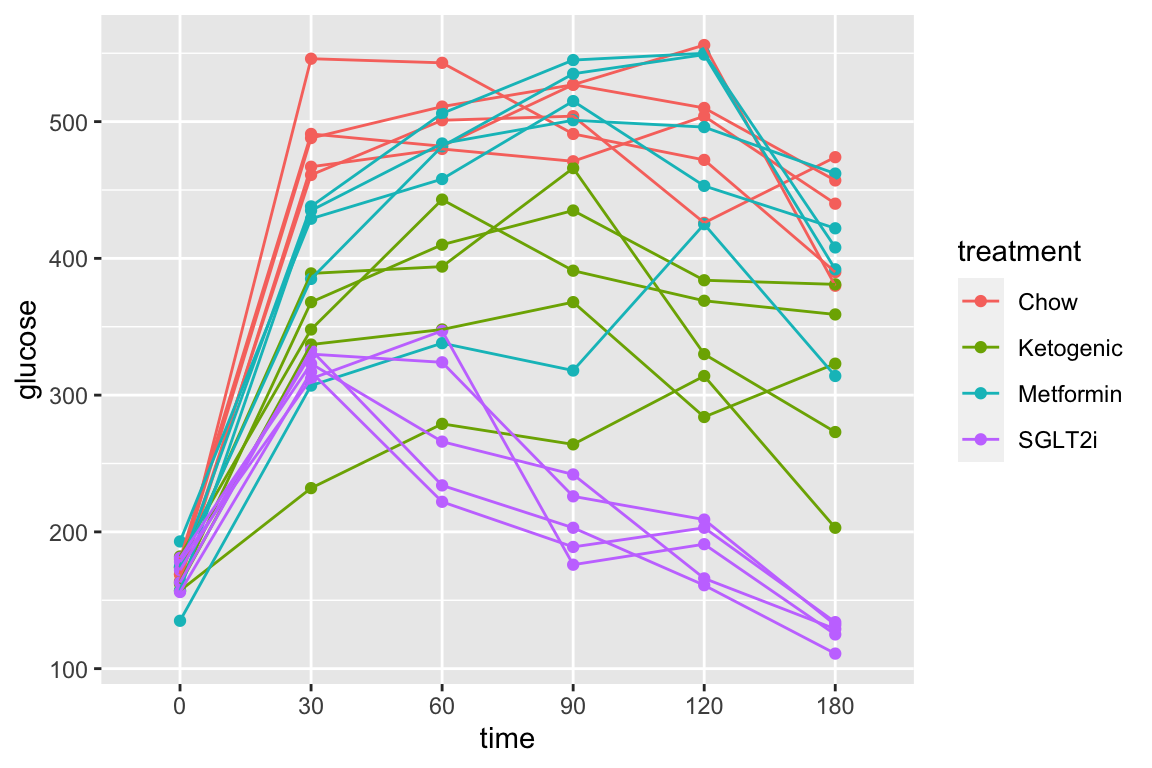
\includegraphics{Walker-elementary-statistical-modeling-draft_files/figure-latex/unnamed-chunk-27-1.pdf}

\hypertarget{figure-2f-effect-of-ask1-on-glucose-infusion-rate}{%
\section{Figure 2f -- Effect of ASK1 on glucose infusion rate}\label{figure-2f-effect-of-ask1-on-glucose-infusion-rate}}

\hypertarget{figure-2f-import}{%
\subsection{Figure 2f -- import}\label{figure-2f-import}}

\begin{Shaded}
\begin{Highlighting}[]
\NormalTok{range_2f <-}\StringTok{ "A239:I240"}
\NormalTok{treatment_levels <-}\StringTok{ }\KeywordTok{c}\NormalTok{(}\StringTok{"ASK1F/F"}\NormalTok{, }\StringTok{"ASK1Δadipo"}\NormalTok{)}
\NormalTok{fig_2f <-}\StringTok{ }\KeywordTok{read_excel}\NormalTok{(file_path,}
                     \DataTypeTok{sheet =}\NormalTok{ fig_}\DecValTok{2}\NormalTok{_sheet,}
                     \DataTypeTok{range =}\NormalTok{ range_2f,}
                     \DataTypeTok{col_names =} \OtherTok{FALSE}\NormalTok{) }\OperatorTok
\StringTok{  }\KeywordTok{transpose}\NormalTok{(}\DataTypeTok{make.names=}\DecValTok{1}\NormalTok{) }\OperatorTok
\StringTok{  }\KeywordTok{data.table}\NormalTok{() }\OperatorTok
\StringTok{  }\KeywordTok{melt}\NormalTok{(}\DataTypeTok{measure.vars =}\NormalTok{ treatment_levels,}
       \DataTypeTok{variable.name =} \StringTok{"treatment"}\NormalTok{,}
       \DataTypeTok{value.name =} \StringTok{"glucose_infusion_rate"}\NormalTok{) }\OperatorTok
\StringTok{  }\KeywordTok{na.omit}\NormalTok{()}

\NormalTok{fig_2f[, treatment }\OperatorTok{:}\ErrorTok{=}\StringTok{ }\KeywordTok{factor}\NormalTok{(treatment, treatment_levels)]}
\end{Highlighting}
\end{Shaded}

\hypertarget{figure-2f-exploratory-plots}{%
\subsection{Figure 2f -- exploratory plots}\label{figure-2f-exploratory-plots}}

\hypertarget{figure-2f-fit-the-model}{%
\subsection{Figure 2f -- fit the model}\label{figure-2f-fit-the-model}}

\begin{Shaded}
\begin{Highlighting}[]
\NormalTok{fig_2f_m1 <-}\StringTok{ }\KeywordTok{lm}\NormalTok{(glucose_infusion_rate }\OperatorTok{~}\StringTok{ }\NormalTok{treatment, }\DataTypeTok{data =}\NormalTok{ fig_2f)}
\end{Highlighting}
\end{Shaded}

\hypertarget{figure-2f-check-the-model}{%
\subsection{Figure 2f -- check the model}\label{figure-2f-check-the-model}}

\hypertarget{figure-2f-inference}{%
\subsection{Figure 2f -- inference}\label{figure-2f-inference}}

\begin{Shaded}
\begin{Highlighting}[]
\NormalTok{fig_2f_m1_coef <-}\StringTok{ }\KeywordTok{summary}\NormalTok{(fig_2f_m1) }\OperatorTok
\StringTok{  }\KeywordTok{coef}\NormalTok{()}
\NormalTok{fig_2f_m1_emm <-}\StringTok{ }\KeywordTok{emmeans}\NormalTok{(fig_2f_m1, }\DataTypeTok{specs =} \StringTok{"treatment"}\NormalTok{)}
\NormalTok{fig_2f_m1_pairs <-}\StringTok{ }\KeywordTok{contrast}\NormalTok{(fig_2f_m1_emm,}
                            \DataTypeTok{method =} \StringTok{"revpairwise"}\NormalTok{) }\OperatorTok
\StringTok{  }\KeywordTok{summary}\NormalTok{(}\DataTypeTok{infer =} \OtherTok{TRUE}\NormalTok{)}
\end{Highlighting}
\end{Shaded}

\begin{Shaded}
\begin{Highlighting}[]
\NormalTok{fig_2f_m1_pairs}
\end{Highlighting}
\end{Shaded}

\begin{verbatim}
##  contrast             estimate  SE df lower.CL upper.CL t.ratio p.value
##  ASK1Δadipo - ASK1F/F     18.9 6.3 12     5.18     32.6 3.000   0.0111 
## 
## Confidence level used: 0.95
\end{verbatim}

\hypertarget{figure-2f-plot-the-model}{%
\subsection{Figure 2f -- plot the model}\label{figure-2f-plot-the-model}}

\begin{Shaded}
\begin{Highlighting}[]
\NormalTok{fig_2f_m1_emm_dt <-}\StringTok{ }\KeywordTok{summary}\NormalTok{(fig_2f_m1_emm) }\OperatorTok
\StringTok{  }\NormalTok{data.table}
\NormalTok{fig_2f_m1_pairs_dt <-}\StringTok{ }\KeywordTok{data.table}\NormalTok{(fig_2f_m1_pairs)}
\NormalTok{fig_2f_m1_pairs_dt[ , p_pretty }\OperatorTok{:}\ErrorTok{=}\StringTok{ }\KeywordTok{pvalString}\NormalTok{(p.value)]}
\NormalTok{fig_2f_m1_pairs_dt[, group1 }\OperatorTok{:}\ErrorTok{=}\StringTok{ }\DecValTok{1}\NormalTok{]}
\NormalTok{fig_2f_m1_pairs_dt[, group2 }\OperatorTok{:}\ErrorTok{=}\StringTok{ }\DecValTok{2}\NormalTok{]}


\NormalTok{fig_2f_gg <-}\StringTok{ }\KeywordTok{ggplot}\NormalTok{(}\DataTypeTok{data =}\NormalTok{ fig_2f,}
                    \KeywordTok{aes}\NormalTok{(}\DataTypeTok{x =}\NormalTok{ treatment,}
                        \DataTypeTok{y =}\NormalTok{ glucose_infusion_rate,}
                        \DataTypeTok{color =}\NormalTok{ treatment)) }\OperatorTok{+}
\StringTok{  }
\StringTok{  }\CommentTok{# points}
\StringTok{  }\KeywordTok{geom_sina}\NormalTok{(}\DataTypeTok{alpha =} \FloatTok{0.5}\NormalTok{,}
            \DataTypeTok{position =}\NormalTok{ pd) }\OperatorTok{+}
\StringTok{  }
\StringTok{  }\CommentTok{# plot means and CI}
\StringTok{  }\KeywordTok{geom_errorbar}\NormalTok{(}\DataTypeTok{data =}\NormalTok{ fig_2f_m1_emm_dt,}
                \KeywordTok{aes}\NormalTok{(}\DataTypeTok{y =}\NormalTok{ emmean,}
                    \DataTypeTok{ymin =}\NormalTok{ lower.CL,}
                    \DataTypeTok{ymax =}\NormalTok{ upper.CL,}
                    \DataTypeTok{color =}\NormalTok{ treatment),}
                \DataTypeTok{width =} \DecValTok{0}\NormalTok{,}
                \DataTypeTok{position =}\NormalTok{ pd,}
                \DataTypeTok{color =} \StringTok{"black"}
\NormalTok{  ) }\OperatorTok{+}
\StringTok{  }
\StringTok{  }\KeywordTok{geom_point}\NormalTok{(}\DataTypeTok{data =}\NormalTok{ fig_2f_m1_emm_dt,}
             \KeywordTok{aes}\NormalTok{(}\DataTypeTok{y =}\NormalTok{ emmean,}
                 \DataTypeTok{color =}\NormalTok{ treatment),}
             \DataTypeTok{size =} \DecValTok{3}\NormalTok{,}
             \DataTypeTok{position =}\NormalTok{ pd,}
             \DataTypeTok{color =} \StringTok{"black"}
\NormalTok{  ) }\OperatorTok{+}
\StringTok{  }
\StringTok{ }\CommentTok{# plot p-values (y positions are adjusted by eye)}
\StringTok{  }\KeywordTok{stat_pvalue_manual}\NormalTok{(fig_2f_m1_pairs_dt,}
                     \DataTypeTok{label =} \StringTok{"p_pretty"}\NormalTok{,}
                     \DataTypeTok{y.position=}\KeywordTok{c}\NormalTok{(}\DecValTok{95}\NormalTok{),}
                     \DataTypeTok{tip.length =} \FloatTok{0.01}\NormalTok{) }\OperatorTok{+}
\StringTok{  }
\StringTok{  }\CommentTok{# aesthetics}
\StringTok{  }\KeywordTok{ylab}\NormalTok{(}\StringTok{"Glucose infusion rate"}\NormalTok{) }\OperatorTok{+}
\StringTok{  }\KeywordTok{scale_color_manual}\NormalTok{(}\DataTypeTok{values=}\NormalTok{pal_nature_mod,}
                     \DataTypeTok{name =} \OtherTok{NULL}\NormalTok{) }\OperatorTok{+}
\StringTok{  }\KeywordTok{theme_pubr}\NormalTok{() }\OperatorTok{+}
\StringTok{  }\KeywordTok{theme}\NormalTok{(}\DataTypeTok{legend.position=}\StringTok{"none"}\NormalTok{) }\OperatorTok{+}
\StringTok{  }\KeywordTok{theme}\NormalTok{(}\DataTypeTok{axis.title.x=}\KeywordTok{element_blank}\NormalTok{()) }\OperatorTok{+}
\StringTok{  }
\StringTok{  }\OtherTok{NULL}

\NormalTok{fig_2f_gg}
\end{Highlighting}
\end{Shaded}

\begin{verbatim}
## Warning in grid.Call(C_textBounds, as.graphicsAnnot(x$label), x$x, x$y, :
## conversion failure on 'ASK1Δadipo' in 'mbcsToSbcs': dot substituted for
## <ce>
\end{verbatim}

\begin{verbatim}
## Warning in grid.Call(C_textBounds, as.graphicsAnnot(x$label), x$x, x$y, :
## conversion failure on 'ASK1Δadipo' in 'mbcsToSbcs': dot substituted for
## <94>
\end{verbatim}

\begin{verbatim}
## Warning in grid.Call(C_textBounds, as.graphicsAnnot(x$label), x$x, x$y, :
## conversion failure on 'ASK1Δadipo' in 'mbcsToSbcs': dot substituted for
## <ce>
\end{verbatim}

\begin{verbatim}
## Warning in grid.Call(C_textBounds, as.graphicsAnnot(x$label), x$x, x$y, :
## conversion failure on 'ASK1Δadipo' in 'mbcsToSbcs': dot substituted for
## <94>
\end{verbatim}

\begin{verbatim}
## Warning in grid.Call(C_textBounds, as.graphicsAnnot(x$label), x$x, x$y, :
## conversion failure on 'ASK1Δadipo' in 'mbcsToSbcs': dot substituted for
## <ce>
\end{verbatim}

\begin{verbatim}
## Warning in grid.Call(C_textBounds, as.graphicsAnnot(x$label), x$x, x$y, :
## conversion failure on 'ASK1Δadipo' in 'mbcsToSbcs': dot substituted for
## <94>
\end{verbatim}

\begin{verbatim}
## Warning in grid.Call(C_textBounds, as.graphicsAnnot(x$label), x$x, x$y, :
## conversion failure on 'ASK1Δadipo' in 'mbcsToSbcs': dot substituted for
## <ce>
\end{verbatim}

\begin{verbatim}
## Warning in grid.Call(C_textBounds, as.graphicsAnnot(x$label), x$x, x$y, :
## conversion failure on 'ASK1Δadipo' in 'mbcsToSbcs': dot substituted for
## <94>
\end{verbatim}

\begin{verbatim}
## Warning in grid.Call(C_textBounds, as.graphicsAnnot(x$label), x$x, x$y, :
## conversion failure on 'ASK1Δadipo' in 'mbcsToSbcs': dot substituted for
## <ce>
\end{verbatim}

\begin{verbatim}
## Warning in grid.Call(C_textBounds, as.graphicsAnnot(x$label), x$x, x$y, :
## conversion failure on 'ASK1Δadipo' in 'mbcsToSbcs': dot substituted for
## <94>
\end{verbatim}

\begin{verbatim}
## Warning in grid.Call(C_textBounds, as.graphicsAnnot(x$label), x$x, x$y, :
## conversion failure on 'ASK1Δadipo' in 'mbcsToSbcs': dot substituted for
## <ce>
\end{verbatim}

\begin{verbatim}
## Warning in grid.Call(C_textBounds, as.graphicsAnnot(x$label), x$x, x$y, :
## conversion failure on 'ASK1Δadipo' in 'mbcsToSbcs': dot substituted for
## <94>
\end{verbatim}

\begin{verbatim}
## Warning in grid.Call(C_textBounds, as.graphicsAnnot(x$label), x$x, x$y, :
## conversion failure on 'ASK1Δadipo' in 'mbcsToSbcs': dot substituted for
## <ce>
\end{verbatim}

\begin{verbatim}
## Warning in grid.Call(C_textBounds, as.graphicsAnnot(x$label), x$x, x$y, :
## conversion failure on 'ASK1Δadipo' in 'mbcsToSbcs': dot substituted for
## <94>
\end{verbatim}

\begin{verbatim}
## Warning in grid.Call(C_textBounds, as.graphicsAnnot(x$label), x$x, x$y, :
## conversion failure on 'ASK1Δadipo' in 'mbcsToSbcs': dot substituted for
## <ce>
\end{verbatim}

\begin{verbatim}
## Warning in grid.Call(C_textBounds, as.graphicsAnnot(x$label), x$x, x$y, :
## conversion failure on 'ASK1Δadipo' in 'mbcsToSbcs': dot substituted for
## <94>
\end{verbatim}

\begin{verbatim}
## Warning in grid.Call(C_textBounds, as.graphicsAnnot(x$label), x$x, x$y, :
## conversion failure on 'ASK1Δadipo' in 'mbcsToSbcs': dot substituted for
## <ce>
\end{verbatim}

\begin{verbatim}
## Warning in grid.Call(C_textBounds, as.graphicsAnnot(x$label), x$x, x$y, :
## conversion failure on 'ASK1Δadipo' in 'mbcsToSbcs': dot substituted for
## <94>
\end{verbatim}

\begin{verbatim}
## Warning in grid.Call(C_textBounds, as.graphicsAnnot(x$label), x$x, x$y, :
## conversion failure on 'ASK1Δadipo' in 'mbcsToSbcs': dot substituted for
## <ce>
\end{verbatim}

\begin{verbatim}
## Warning in grid.Call(C_textBounds, as.graphicsAnnot(x$label), x$x, x$y, :
## conversion failure on 'ASK1Δadipo' in 'mbcsToSbcs': dot substituted for
## <94>
\end{verbatim}

\begin{verbatim}
## Warning in grid.Call(C_textBounds, as.graphicsAnnot(x$label), x$x, x$y, :
## conversion failure on 'ASK1Δadipo' in 'mbcsToSbcs': dot substituted for
## <ce>
\end{verbatim}

\begin{verbatim}
## Warning in grid.Call(C_textBounds, as.graphicsAnnot(x$label), x$x, x$y, :
## conversion failure on 'ASK1Δadipo' in 'mbcsToSbcs': dot substituted for
## <94>
\end{verbatim}

\begin{verbatim}
## Warning in grid.Call(C_textBounds, as.graphicsAnnot(x$label), x$x, x$y, :
## conversion failure on 'ASK1Δadipo' in 'mbcsToSbcs': dot substituted for
## <ce>
\end{verbatim}

\begin{verbatim}
## Warning in grid.Call(C_textBounds, as.graphicsAnnot(x$label), x$x, x$y, :
## conversion failure on 'ASK1Δadipo' in 'mbcsToSbcs': dot substituted for
## <94>
\end{verbatim}

\begin{verbatim}
## Warning in grid.Call(C_textBounds, as.graphicsAnnot(x$label), x$x, x$y, :
## conversion failure on 'ASK1Δadipo' in 'mbcsToSbcs': dot substituted for
## <ce>
\end{verbatim}

\begin{verbatim}
## Warning in grid.Call(C_textBounds, as.graphicsAnnot(x$label), x$x, x$y, :
## conversion failure on 'ASK1Δadipo' in 'mbcsToSbcs': dot substituted for
## <94>
\end{verbatim}

\begin{verbatim}
## Warning in grid.Call.graphics(C_text, as.graphicsAnnot(x$label), x$x,
## x$y, : conversion failure on 'ASK1Δadipo' in 'mbcsToSbcs': dot substituted
## for <ce>
\end{verbatim}

\begin{verbatim}
## Warning in grid.Call.graphics(C_text, as.graphicsAnnot(x$label), x$x,
## x$y, : conversion failure on 'ASK1Δadipo' in 'mbcsToSbcs': dot substituted
## for <94>
\end{verbatim}

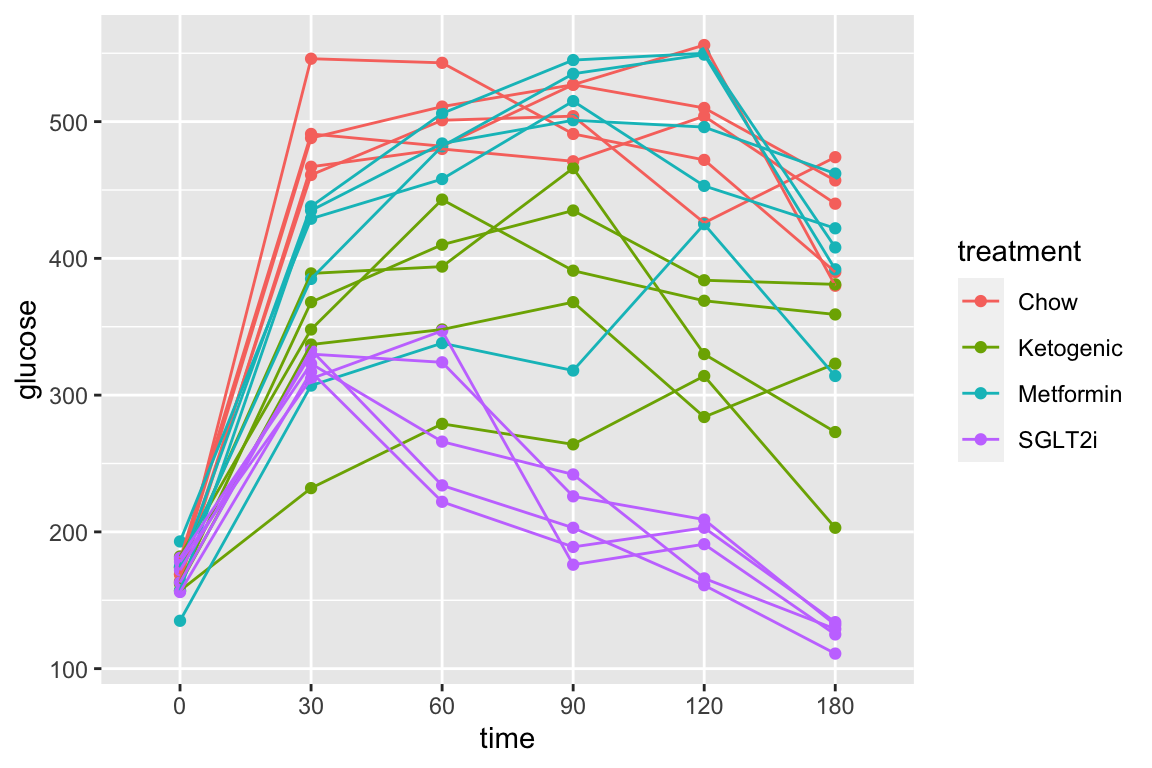
\includegraphics{Walker-elementary-statistical-modeling-draft_files/figure-latex/unnamed-chunk-32-1.pdf}

\hypertarget{figure-2g}{%
\section{Figure 2g}\label{figure-2g}}

\hypertarget{figure-2g-import}{%
\subsection{Figure 2g -- import}\label{figure-2g-import}}

\begin{Shaded}
\begin{Highlighting}[]
\NormalTok{range_list <-}\StringTok{ }\KeywordTok{c}\NormalTok{(}\StringTok{"A244:G247"}\NormalTok{, }\StringTok{"A250:H253"}\NormalTok{)}
\CommentTok{# import ASK1F/F}
\NormalTok{fig_2g_}\DecValTok{1}\NormalTok{ <-}\StringTok{ }\KeywordTok{read_excel}\NormalTok{(file_path,}
                     \DataTypeTok{sheet =}\NormalTok{ fig_}\DecValTok{2}\NormalTok{_sheet,}
                     \DataTypeTok{range =} \StringTok{"A244:G247"}\NormalTok{,}
                     \DataTypeTok{col_names =} \OtherTok{FALSE}\NormalTok{) }\OperatorTok
\StringTok{  }\KeywordTok{transpose}\NormalTok{(}\DataTypeTok{make.names=}\DecValTok{1}\NormalTok{) }\OperatorTok
\StringTok{  }\KeywordTok{data.table}\NormalTok{()}
\end{Highlighting}
\end{Shaded}

\begin{verbatim}
## New names:
## * `` -> ...1
## * `` -> ...2
## * `` -> ...3
## * `` -> ...4
## * `` -> ...5
## * ...
\end{verbatim}

\begin{Shaded}
\begin{Highlighting}[]
\NormalTok{fig_2g_}\DecValTok{1}\NormalTok{[, treatment }\OperatorTok{:}\ErrorTok{=}\StringTok{ "ASK1F/F"}\NormalTok{]}

\CommentTok{# import ASK1Δadipo}
\NormalTok{fig_2g_}\DecValTok{2}\NormalTok{ <-}\StringTok{ }\KeywordTok{read_excel}\NormalTok{(file_path,}
                     \DataTypeTok{sheet =}\NormalTok{ fig_}\DecValTok{2}\NormalTok{_sheet,}
                     \DataTypeTok{range =} \StringTok{"A250:H253"}\NormalTok{,}
                     \DataTypeTok{col_names =} \OtherTok{FALSE}\NormalTok{) }\OperatorTok
\StringTok{  }\KeywordTok{transpose}\NormalTok{(}\DataTypeTok{make.names=}\DecValTok{1}\NormalTok{) }\OperatorTok
\StringTok{  }\KeywordTok{data.table}\NormalTok{()}
\end{Highlighting}
\end{Shaded}

\begin{verbatim}
## New names:
## * `` -> ...1
## * `` -> ...2
## * `` -> ...3
## * `` -> ...4
## * `` -> ...5
## * ...
\end{verbatim}

\begin{Shaded}
\begin{Highlighting}[]
\NormalTok{fig_2g_}\DecValTok{2}\NormalTok{[, treatment }\OperatorTok{:}\ErrorTok{=}\StringTok{ "ASK1Δadipo"}\NormalTok{]}

\CommentTok{# combine}
\NormalTok{fig_2g <-}\StringTok{ }\KeywordTok{rbind}\NormalTok{(fig_2g_}\DecValTok{1}\NormalTok{, fig_2g_}\DecValTok{2}\NormalTok{)}
\end{Highlighting}
\end{Shaded}

\hypertarget{figure-2g-exploratory-plots}{%
\subsection{Figure 2g -- exploratory plots}\label{figure-2g-exploratory-plots}}

\hypertarget{figure-2g-fit-the-model}{%
\subsection{Figure 2g -- fit the model}\label{figure-2g-fit-the-model}}

\begin{Shaded}
\begin{Highlighting}[]
\CommentTok{# a more sophisticated would be a mixed model to dampen noise}
\NormalTok{fig_2g_m1_ingWAT <-}\StringTok{ }\KeywordTok{lm}\NormalTok{(ingWAT }\OperatorTok{~}\StringTok{ }\NormalTok{treatment, }\DataTypeTok{data =}\NormalTok{ fig_2g)}
\NormalTok{fig_2g_m1_epiWAT <-}\StringTok{ }\KeywordTok{lm}\NormalTok{(epiWAT }\OperatorTok{~}\StringTok{ }\NormalTok{treatment, }\DataTypeTok{data =}\NormalTok{ fig_2g)}
\NormalTok{fig_2g_m1_Muscle <-}\StringTok{ }\KeywordTok{lm}\NormalTok{(Muscle }\OperatorTok{~}\StringTok{ }\NormalTok{treatment, }\DataTypeTok{data =}\NormalTok{ fig_2g)}
\NormalTok{fig_2g_m1_BAT <-}\StringTok{ }\KeywordTok{lm}\NormalTok{(BAT }\OperatorTok{~}\StringTok{ }\NormalTok{treatment, }\DataTypeTok{data =}\NormalTok{ fig_2g)}
\end{Highlighting}
\end{Shaded}

\hypertarget{figure-2g-check-the-model}{%
\subsection{Figure 2g -- check the model}\label{figure-2g-check-the-model}}

\hypertarget{figure-2g-inference}{%
\subsection{Figure 2g -- inference}\label{figure-2g-inference}}

\begin{Shaded}
\begin{Highlighting}[]
\NormalTok{fig_2g_infer <-}\StringTok{ }\ControlFlowTok{function}\NormalTok{(m1)\{}
\NormalTok{  m1_emm <-}\StringTok{ }\KeywordTok{emmeans}\NormalTok{(m1, }\DataTypeTok{specs =} \StringTok{"treatment"}\NormalTok{)}
\NormalTok{  m1_pairs <-}\StringTok{ }\KeywordTok{contrast}\NormalTok{(m1_emm,}
                              \DataTypeTok{method =} \StringTok{"revpairwise"}\NormalTok{) }\OperatorTok
\StringTok{    }\KeywordTok{summary}\NormalTok{(}\DataTypeTok{infer =} \OtherTok{TRUE}\NormalTok{)}
  \KeywordTok{return}\NormalTok{(}\KeywordTok{list}\NormalTok{(}\DataTypeTok{emm =}\NormalTok{ m1_emm,}
              \DataTypeTok{pairs =}\NormalTok{ m1_pairs))}
\NormalTok{\}}

\NormalTok{fig_2g_m1_emm_dt <-}\StringTok{ }\KeywordTok{data.table}\NormalTok{(}\OtherTok{NULL}\NormalTok{)}
\NormalTok{fig_2g_m1_pairs_dt <-}\StringTok{ }\KeywordTok{data.table}\NormalTok{(}\OtherTok{NULL}\NormalTok{)}
\NormalTok{m1_list <-}\StringTok{ }\KeywordTok{list}\NormalTok{(fig_2g_m1_ingWAT, }
\NormalTok{             fig_2g_m1_epiWAT,}
\NormalTok{             fig_2g_m1_Muscle,}
\NormalTok{             fig_2g_m1_BAT)}
\NormalTok{y_cols <-}\StringTok{ }\KeywordTok{c}\NormalTok{(}\StringTok{"ingWAT"}\NormalTok{, }\StringTok{"epiWAT"}\NormalTok{, }\StringTok{"Muscle"}\NormalTok{, }\StringTok{"BAT"}\NormalTok{)}
\ControlFlowTok{for}\NormalTok{(i }\ControlFlowTok{in} \DecValTok{1}\OperatorTok{:}\KeywordTok{length}\NormalTok{(y_cols))\{}
\NormalTok{  m1_infer <-}\StringTok{ }\KeywordTok{fig_2g_infer}\NormalTok{(m1_list[[i]])}

\NormalTok{  m1_emm_dt <-}\StringTok{ }\KeywordTok{summary}\NormalTok{(m1_infer}\OperatorTok{$}\NormalTok{emm) }\OperatorTok
\StringTok{    }\NormalTok{data.table}
\NormalTok{  fig_2g_m1_emm_dt <-}\StringTok{ }\KeywordTok{rbind}\NormalTok{(fig_2g_m1_emm_dt,}
                            \KeywordTok{data.table}\NormalTok{(}\DataTypeTok{tissue =}\NormalTok{ y_cols[i], m1_emm_dt))}
\NormalTok{  m1_pairs_dt <-}\StringTok{ }\NormalTok{m1_infer}\OperatorTok{$}\NormalTok{pairs }\OperatorTok
\StringTok{    }\NormalTok{data.table}
\NormalTok{  fig_2g_m1_pairs_dt <-}\StringTok{ }\KeywordTok{rbind}\NormalTok{(fig_2g_m1_pairs_dt,}
                            \KeywordTok{data.table}\NormalTok{(}\DataTypeTok{tissue =}\NormalTok{ y_cols[i], m1_pairs_dt))}
\NormalTok{\}}
\end{Highlighting}
\end{Shaded}

\begin{Shaded}
\begin{Highlighting}[]
\NormalTok{fig_2g_m1_pairs_dt}
\end{Highlighting}
\end{Shaded}

\begin{verbatim}
##    tissue             contrast  estimate        SE df     lower.CL
## 1: ingWAT ASK1Δadipo - ASK1F/F  3.595000  1.468289 10   0.32344725
## 2: epiWAT ASK1Δadipo - ASK1F/F  1.390238  0.669957 11  -0.08432738
## 3: Muscle ASK1Δadipo - ASK1F/F  2.694048  5.675468 11  -9.79757382
## 4:    BAT ASK1Δadipo - ASK1F/F 33.855000 28.715230  7 -34.04572935
##      upper.CL   t.ratio    p.value
## 1:   6.866553 2.4484273 0.03435010
## 2:   2.864804 2.0751153 0.06222096
## 3:  15.185669 0.4746829 0.64429728
## 4: 101.755729 1.1789911 0.27691810
\end{verbatim}

\hypertarget{figure-2g-plot-the-model}{%
\subsection{Figure 2g -- plot the model}\label{figure-2g-plot-the-model}}

\begin{Shaded}
\begin{Highlighting}[]
\CommentTok{# melt fig_2g}

\NormalTok{fig_2g_long <-}\StringTok{ }\KeywordTok{melt}\NormalTok{(fig_2g,}
                    \DataTypeTok{id.vars =} \StringTok{"treatment"}\NormalTok{,}
                    \DataTypeTok{variable.name =} \StringTok{"tissue"}\NormalTok{,}
                    \DataTypeTok{value.name =} \StringTok{"glucose_uptake"}\NormalTok{)}

\CommentTok{# change name of ASK1Δadipo label}
\NormalTok{fig_2g_long[treatment }\OperatorTok{==}\StringTok{ "ASK1Δadipo"}\NormalTok{, treatment }\OperatorTok{:}\ErrorTok{=}\StringTok{ "ASK1-/-adipo"}\NormalTok{]}
\NormalTok{fig_2g_m1_emm_dt[treatment }\OperatorTok{==}\StringTok{ "ASK1Δadipo"}\NormalTok{, treatment }\OperatorTok{:}\ErrorTok{=}\StringTok{ "ASK1-/-adipo"}\NormalTok{]}

\NormalTok{fig_2g_m1_pairs_dt[ , p_pretty }\OperatorTok{:}\ErrorTok{=}\StringTok{ }\KeywordTok{pvalString}\NormalTok{(p.value)]}
\NormalTok{fig_2g_m1_pairs_dt[, group1 }\OperatorTok{:}\ErrorTok{=}\StringTok{ }\DecValTok{1}\NormalTok{]}
\NormalTok{fig_2g_m1_pairs_dt[, group2 }\OperatorTok{:}\ErrorTok{=}\StringTok{ }\DecValTok{2}\NormalTok{]}

\NormalTok{fig_2g_plot <-}\StringTok{ }\ControlFlowTok{function}\NormalTok{(tissue_i,}
                        \DataTypeTok{y_lab =} \OtherTok{FALSE}\NormalTok{, }\CommentTok{# title y-axis?}
                        \DataTypeTok{g_lab =} \OtherTok{FALSE}  \CommentTok{# add group label?}
\NormalTok{                        )\{}
\NormalTok{  y_max <-}\StringTok{ }\KeywordTok{max}\NormalTok{(fig_2g_long[tissue }\OperatorTok{==}\StringTok{ }\NormalTok{tissue_i, glucose_uptake], }\DataTypeTok{na.rm=}\OtherTok{TRUE}\NormalTok{)}
\NormalTok{  y_min <-}\StringTok{ }\KeywordTok{min}\NormalTok{(fig_2g_long[tissue }\OperatorTok{==}\StringTok{ }\NormalTok{tissue_i, glucose_uptake], }\DataTypeTok{na.rm=}\OtherTok{TRUE}\NormalTok{)}
\NormalTok{  y_pos <-}\StringTok{ }\NormalTok{y_max }\OperatorTok{+}\StringTok{ }\NormalTok{(y_max}\OperatorTok{-}\NormalTok{y_min)}\OperatorTok{*}\NormalTok{.}\DecValTok{05}
  
\NormalTok{  gg <-}\StringTok{ }\KeywordTok{ggplot}\NormalTok{(}\DataTypeTok{data =}\NormalTok{ fig_2g_long[tissue }\OperatorTok{==}\StringTok{ }\NormalTok{tissue_i],}
                      \KeywordTok{aes}\NormalTok{(}\DataTypeTok{x =}\NormalTok{ treatment,}
                          \DataTypeTok{y =}\NormalTok{ glucose_uptake,}
                          \DataTypeTok{color =}\NormalTok{ treatment)) }\OperatorTok{+}
\StringTok{    }
\StringTok{    }\CommentTok{# points}
\StringTok{    }\KeywordTok{geom_sina}\NormalTok{(}\DataTypeTok{alpha =} \FloatTok{0.5}\NormalTok{,}
              \DataTypeTok{position =}\NormalTok{ pd) }\OperatorTok{+}
\StringTok{    }
\StringTok{    }\CommentTok{# plot means and CI}
\StringTok{    }\KeywordTok{geom_errorbar}\NormalTok{(}\DataTypeTok{data =}\NormalTok{ fig_2g_m1_emm_dt[tissue }\OperatorTok{==}\StringTok{ }\NormalTok{tissue_i],}
                  \KeywordTok{aes}\NormalTok{(}\DataTypeTok{y =}\NormalTok{ emmean,}
                      \DataTypeTok{ymin =}\NormalTok{ lower.CL,}
                      \DataTypeTok{ymax =}\NormalTok{ upper.CL,}
                      \DataTypeTok{color =}\NormalTok{ treatment),}
                  \DataTypeTok{width =} \DecValTok{0}\NormalTok{,}
                  \DataTypeTok{position =}\NormalTok{ pd}
\NormalTok{    ) }\OperatorTok{+}
\StringTok{    }
\StringTok{    }\KeywordTok{geom_point}\NormalTok{(}\DataTypeTok{data =}\NormalTok{ fig_2g_m1_emm_dt[tissue }\OperatorTok{==}\StringTok{ }\NormalTok{tissue_i],}
               \KeywordTok{aes}\NormalTok{(}\DataTypeTok{y =}\NormalTok{ emmean,}
                   \DataTypeTok{color =}\NormalTok{ treatment),}
               \DataTypeTok{size =} \DecValTok{3}\NormalTok{,}
               \DataTypeTok{position =}\NormalTok{ pd}
\NormalTok{    ) }\OperatorTok{+}
\StringTok{    }
\StringTok{    }\CommentTok{# plot p-values (y positions are adjusted by eye)}
\StringTok{    }\KeywordTok{stat_pvalue_manual}\NormalTok{(fig_2g_m1_pairs_dt[tissue }\OperatorTok{==}\StringTok{ }\NormalTok{tissue_i],}
                       \DataTypeTok{label =} \StringTok{"p_pretty"}\NormalTok{,}
                       \DataTypeTok{y.position=}\KeywordTok{c}\NormalTok{(y_pos),}
                       \DataTypeTok{tip.length =} \FloatTok{0.01}\NormalTok{) }\OperatorTok{+}
\StringTok{    }
\StringTok{    }\CommentTok{# aesthetics}
\StringTok{    }\KeywordTok{ylab}\NormalTok{(}\StringTok{"Glucose Uptake"}\NormalTok{) }\OperatorTok{+}
\StringTok{    }\KeywordTok{scale_color_manual}\NormalTok{(}\DataTypeTok{values=}\NormalTok{pal_nature_mod,}
                       \DataTypeTok{name =} \OtherTok{NULL}\NormalTok{) }\OperatorTok{+}
\StringTok{    }\KeywordTok{ggtitle}\NormalTok{(tissue_i)}\OperatorTok{+}
\StringTok{    }
\StringTok{    }\KeywordTok{theme_pubr}\NormalTok{() }\OperatorTok{+}
\StringTok{    }\KeywordTok{theme}\NormalTok{(}\DataTypeTok{legend.position=}\StringTok{"top"}\NormalTok{) }\OperatorTok{+}
\StringTok{    }\KeywordTok{theme}\NormalTok{(}\DataTypeTok{axis.title.x =} \KeywordTok{element_blank}\NormalTok{(),}
          \DataTypeTok{axis.text.x =} \KeywordTok{element_blank}\NormalTok{(),}
          \DataTypeTok{axis.ticks.x =} \KeywordTok{element_blank}\NormalTok{()) }\OperatorTok{+}
\StringTok{    }
\StringTok{    }\OtherTok{NULL}
  
  \ControlFlowTok{if}\NormalTok{(y_lab }\OperatorTok{==}\StringTok{ }\OtherTok{FALSE}\NormalTok{)\{}
\NormalTok{    gg <-}\StringTok{ }\NormalTok{gg }\OperatorTok{+}\StringTok{ }\KeywordTok{theme}\NormalTok{(}\DataTypeTok{axis.title.y =} \KeywordTok{element_blank}\NormalTok{())}
\NormalTok{  \}}
  \ControlFlowTok{if}\NormalTok{(g_lab }\OperatorTok{==}\StringTok{ }\OtherTok{FALSE}\NormalTok{)\{}
\NormalTok{    gg <-}\StringTok{ }\NormalTok{gg }\OperatorTok{+}\StringTok{ }\KeywordTok{theme}\NormalTok{(}\DataTypeTok{legend.position=}\StringTok{"none"}\NormalTok{)}
\NormalTok{  \}}
  
  \KeywordTok{return}\NormalTok{(gg)}
\NormalTok{\}}

\NormalTok{y_cols <-}\StringTok{ }\KeywordTok{c}\NormalTok{(}\StringTok{"ingWAT"}\NormalTok{, }\StringTok{"epiWAT"}\NormalTok{, }\StringTok{"Muscle"}\NormalTok{, }\StringTok{"BAT"}\NormalTok{)}
\NormalTok{legend <-}\StringTok{ }\KeywordTok{get_legend}\NormalTok{(}\KeywordTok{fig_2g_plot}\NormalTok{(}\StringTok{"ingWAT"}\NormalTok{, }\DataTypeTok{y_lab =} \OtherTok{TRUE}\NormalTok{, }\DataTypeTok{g_lab =} \OtherTok{TRUE}\NormalTok{))}
\NormalTok{gg1 <-}\StringTok{ }\KeywordTok{fig_2g_plot}\NormalTok{(}\StringTok{"ingWAT"}\NormalTok{, }\DataTypeTok{y_lab =} \OtherTok{TRUE}\NormalTok{, )}
\NormalTok{gg2 <-}\StringTok{ }\KeywordTok{fig_2g_plot}\NormalTok{(}\StringTok{"epiWAT"}\NormalTok{)}
\NormalTok{gg3 <-}\StringTok{ }\KeywordTok{fig_2g_plot}\NormalTok{(}\StringTok{"Muscle"}\NormalTok{)}
\NormalTok{gg4 <-}\StringTok{ }\KeywordTok{fig_2g_plot}\NormalTok{(}\StringTok{"BAT"}\NormalTok{)}
\NormalTok{top_gg <-}\StringTok{ }\KeywordTok{plot_grid}\NormalTok{(gg1, gg2, gg3, gg4,}
                       \DataTypeTok{nrow=}\DecValTok{1}\NormalTok{,}
                       \DataTypeTok{rel_widths =} \KeywordTok{c}\NormalTok{(}\FloatTok{1.15}\NormalTok{, }\DecValTok{1}\NormalTok{, }\FloatTok{1.05}\NormalTok{, }\FloatTok{1.1}\NormalTok{)) }\CommentTok{# by eye}
\KeywordTok{plot_grid}\NormalTok{(top_gg, legend,}
          \DataTypeTok{nrow=}\DecValTok{2}\NormalTok{,}
          \DataTypeTok{rel_heights =} \KeywordTok{c}\NormalTok{(}\DecValTok{1}\NormalTok{, }\FloatTok{0.1}\NormalTok{))}
\end{Highlighting}
\end{Shaded}

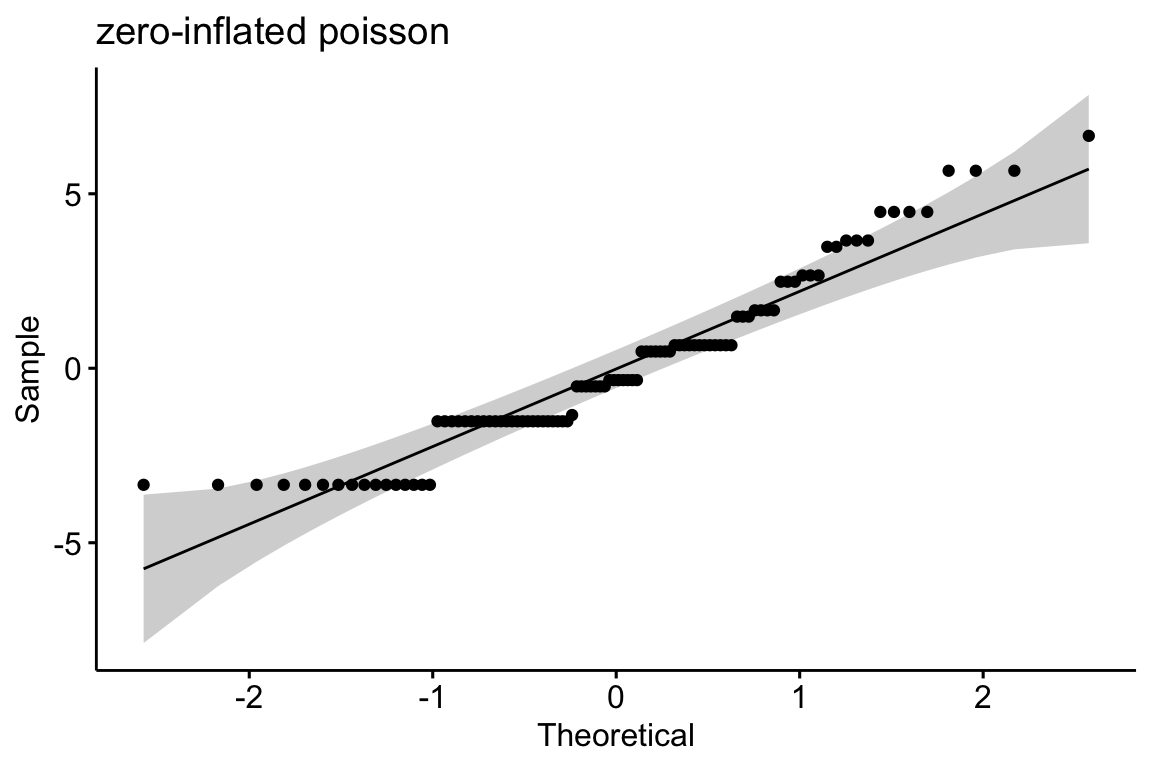
\includegraphics{Walker-elementary-statistical-modeling-draft_files/figure-latex/unnamed-chunk-37-1.pdf}

\hypertarget{figure-2h}{%
\section{Figure 2h}\label{figure-2h}}

\hypertarget{figure-2i}{%
\section{Figure 2i}\label{figure-2i}}

\hypertarget{figure-2j}{%
\section{Figure 2j}\label{figure-2j}}

\hypertarget{exercises}{%
\section{Exercises}\label{exercises}}

\begin{enumerate}
\def\labelenumi{\arabic{enumi}.}
\tightlist
\item
  Using the code chunks for Figure 2f, complete the analysis for Figure 2i. This should simply require copying the chunks from 2f and swapping out the correct names (and the range of the Excel file!) of variables. At a minimum you will need to run
\end{enumerate}

\begin{itemize}
\tightlist
\item
  the setup chunk with the libraries
\item
  the chunk defining the path of the data folder and the sheet with Figure 2
\item
  the chunk defining the pal\_nature\_mod palette in the ``useful functions'' section
\end{itemize}

\hypertarget{part-i-r-fundamentals}{%
\chapter*{Part I: R fundamentals}\label{part-i-r-fundamentals}}
\addcontentsline{toc}{chapter}{Part I: R fundamentals}

\hypertarget{organization-r-projects-and-r-notebooks}{%
\chapter{Organization -- R Projects and R Notebooks}\label{organization-r-projects-and-r-notebooks}}

A typical statistical modeling project will consist of:

\begin{enumerate}
\def\labelenumi{\arabic{enumi}.}
\tightlist
\item
  importing data from Excel or text (.csv or .txt) files
\item
  cleaning data
\item
  initial exploratory plots
\item
  analysis
\item
  model checking
\item
  generating plots
\item
  generating tables
\item
  writing text to describe the project, the methods, the analysis, and the interpretation of the results (plots and tables)
\end{enumerate}

The best practice for reproducible research is to have all of these steps in a single document and all of the files for this project in a single folder (directory), preferably on a cloud drive. Too many research projects are not reproducible because the data were cleaned in Excel, and then different parts of the data were separately imported into a GUI statistics software for analysis, and then output from the statistics software was transcribed to Excel to make a table. And other parts of the analysis are used to create a plot in some plotting software. And then the tables and plots are pasted into Microsoft Word to create a report. Any change at any step in this process will require the researcher to remember all the downstream parts that are dependent on the change and to re-do an analysis, or a table, or a plot, etc. etc.

R studio encourages best practices by creating a \textbf{project folder} that contains all project documents and implementing a version of markdown called R Markdown. An R Markdown document can explicitly link all parts of the workflow so that changes in earlier steps automatically flow into the later steps. At the completion of a project, a researcher can choose ``run all'' from the menu and the data are read, cleaned, analyzed, ploted, tabled, and put into a report with the text.

\hypertarget{r-vs-r-studio}{%
\section{R vs R Studio}\label{r-vs-r-studio}}

R is a programming language. The software that translates this language into instructions for your computer works behind the curtain. To use R, you need some kind of interface software. R Studio is the interface software used in this text. R Studio has options for creating multiple document types that can interface with R. This text uses R Markdown documents, but interestingly R Studio provides two kinds of R Markdown document -- ``R Markdown'' and ``R Notebook''

\hypertarget{r-notebook-vs.-r-markdown}{%
\section{R Notebook vs.~R Markdown}\label{r-notebook-vs.-r-markdown}}

Markdown is a document processing tool for writing single documents that contain text (word processing), code, images, and tables in a single file that can then be \textbf{knit} to all the modern output formats including html for web pages, pdf for technical reports or submissions to journals, and microsoft word for professors or colleagues who are stuck in 1999.

R Markdown is R Studio's version of Markdown. If an R Markdown document is knitted to an html document and opened in a web browser, you will see a pretty web page with your text, code, and images. If the html file is opened in R Studio, you will see a text document of the html code. You won't see pretty text or images or even your R code.

An R Studio Notebook is an R Markdown file. The file is saved with the .Rmd extension like any R markdown file. An R Studio Notebook automatically creates an preview file with the extension .nb.html. If the nb.html file is opened in a web browser, you will see a pretty web page with your text, code, and images -- just like a normal .html file knitted from a normal R Markdown document. But if the .nb.html file is opened in R Studio, you will see the original R Markdown document. Neat!

R Studio Notebooks have advantages and disadvantages. If I use R Markdown to analyze data for a colleague, I can give the colleague the knitted .html file as a beautiful, readable report. In a typical report to colleagues, I will probably hide all the underlying code used to import and wrangle the data, do the computations, and construct the figures. If a colleague wants the underlying code, I have to send the original .Rmd file with the .html file. Or I have to knit two versions of the .html file, a pretty one without all the code chunks and the complete one, with all the code chunks.

If I create my report using an R Studio Notebook and knit to a .nb.html file, then the colleague can see both with a single file! If they only want to read the text and see the pretty images and tables, they can just open the .nb.html file in a browser. But if they want to see the code that did everything, they can open the file in R Studio. Awesome!

An R Studio Notebook is the good tool for a student in a class. The student can send the professor the .nb.html file and the professor can recover the full R Markdown document if needed.

When would I not use R Studio Notebooks? One example is teaching. If I create an assignment where students have to import data, wrangle the data, analyze the data, and create a plot and table, I might give them an .html file with the target image and table\ldots can they reproduce this? I'd create the assignment as an R Markdown document and include code chunks that do everything -- import, wrangle, analyze, plot, table. For the output html, I'd hide the chunks that do all this. If compiled from a R Markdown document, a student could not recover the hidden code. But if compiled from a R Studio notebook document, the student could simply open the .nb.html file in R Studio and recover the original R Markdown document! Don't do this!

Some other differences between R Markdown and R Notebook

The preview (.nb.html) file for a R Notebook is made and updated when the notebook file is saves and includes whatever has been run in the R Notebook document. If a chunk that creates a plot has not been run, the preview file will not show the plot. If a chunk returns messages or warnings, the html preview will show these messages or warnings. This can create a very messy html document to give to a colleague or professor. To hide the messages and warnings, the chunk options ``message=FALSE'' or ``warning=FALSE'' have to be added to each chunk with a message or warning and then the chunk has to be re-run. Now the preview file is clean.

This behavior is very different from knitting a R Markdown file. When knit, all chunks are run so if a chunk creating a plot was not manually run, the chunk will be run during the knit and the plot will show in the output. Since knitting runs all chunks, a user can create global behavior such as inserting \texttt{knitr::opts\_chunk\$set(message\ =\ FALSE)} into the setup chunk. Now a chunk that returns a message when run interactively will not show the message in the knit output. But if I insert this into the setup chunk of an R Notebook document, it will have no effect on the preview because the preview is not a knit file from a clean run of all chunks but a knit file of what the user has done. I sometimes want to see messages and especially warnings when I interact with my chunks but I almost never want these messages in my output. This is easier to do with R Markdown instead of R Notebook because of this ability to set global options.

\hypertarget{importing-packages}{%
\section{Importing Packages}\label{importing-packages}}

The R scripts you write will include functions in packages that are not included in Base R. These packages need to be downloaded from an internet server to your computer. You only need to do this once (although you have to redo it each time you update R). But, each time you start a new R session, you will need to load a package using the \texttt{library()} function. Now is a good time to import packages that we will use

Open R Studio and choose the menu item ``Tools'' \textgreater{} ``Install Packages''. In the ``packages'' input box, insert the names of packages to install the package. The names can be separated by spaces or commas, for example ``data.table, emmeans, ggplot2''. Make sure that ``install dependencies'' is clicked before you click ``Install''. Packages that we will use in this book are

\begin{enumerate}
\def\labelenumi{\arabic{enumi}.}
\tightlist
\item
  Import and analysis packages
\end{enumerate}

\begin{itemize}
\tightlist
\item
  here -- we use to read from and write to the correct folder
\item
  janitor -- we use the function clean\_names from this package
\item
  readxl -- elegant importing from microsoft Excel spreadsheets
\item
  data.table - improves functionality of data frames
\end{itemize}

\begin{enumerate}
\def\labelenumi{\arabic{enumi}.}
\setcounter{enumi}{1}
\tightlist
\item
  analysis packages
\end{enumerate}

\begin{itemize}
\tightlist
\item
  nlme -- we use this for gls models
\item
  lme4 -- we use this for linear mixed models
\item
  lmerTest -- we use this for inference with linear mixed models
\item
  glmmTMB -- we use this for generalized linear models
\item
  MASS -- we will use glm.nb from this package
\item
  afex -- we use this for classic ANOVA
\item
  emmeans -- we use this to compute modeled means and contrasts
\end{itemize}

\begin{enumerate}
\def\labelenumi{\arabic{enumi}.}
\setcounter{enumi}{2}
\tightlist
\item
  graphing packages
\end{enumerate}

\begin{itemize}
\tightlist
\item
  ggplot2 -- we use this for plotting
\item
  ggsci -- we use this for the color palettes
\item
  ggpubr -- we use this to make ggplots a bit easier
\item
  ggforce -- we use this for improved jitter plots
\item
  cowplot -- we use this to combine plots
\end{itemize}

Once these are installed, you don't need to do this again. You simply need to use the \texttt{library()} function at the start of a markdown script.

\hypertarget{create-an-r-studio-project-for-this-textbook}{%
\section{Create an R Studio Project for this textbook}\label{create-an-r-studio-project-for-this-textbook}}

\begin{enumerate}
\def\labelenumi{\arabic{enumi}.}
\tightlist
\item
  Create a project folder within the Documents folder (Mac OS) or My Documents folder (Windows OS). All files associated with this book will reside inside this folder. The name of the project folder should be something meaningful, such as ``Applied\_Biostatics'' or the name of your class (for students in my Applied Biostatics class, this folder could be named ``BIO\_413'').
\item
  Within the project folder, create new folders named

  \begin{enumerate}
  \def\labelenumii{\arabic{enumii}.}
  \tightlist
  \item
    ``Rmd'' -- this is where your R markdown files are stored
  \item
    ``R'' -- this is where additional R script files are stored
  \item
    ``data'' -- this is where data that we download from public archives are stored
  \item
    ``output'' -- this is where you will store fake data generated in this class
  \item
    ``images'' -- this is where image files are stored
  \end{enumerate}
\item
  Open R Studio and click the menu item File \textgreater{} New Project\ldots{}
\item
  Choose ``Existing Directory'' and navigate to your project folder
\item
  Choose ``Create Project''
\item
  Check that a ``.Rproj'' file is in your project folder
\end{enumerate}

\hypertarget{create-an-r-markdown-file-for-this-chapter}{%
\subsection{Create an R Markdown file for this Chapter}\label{create-an-r-markdown-file-for-this-chapter}}

\begin{enumerate}
\def\labelenumi{\arabic{enumi}.}
\tightlist
\item
  The top-left icon in R Studio is a little plus sign within a green circle. Click this and choose ``R Markdown'' from the pull-down menu.
\item
  Give the file a meaningful title like ``Chapter 1 -- Organization''
\item
  Delete all text below the first code chunk, starting with the header ``\#\# R Markdown''
\end{enumerate}

\hypertarget{modify-the-yaml-header}{%
\subsubsection{Modify the yaml header}\label{modify-the-yaml-header}}

Replace ``output: html\_document'' in the yaml header with the following

\begin{verbatim}
output:
  html_document:
    toc: true
    toc_float: true
    code_folding: hide
\end{verbatim}

\hypertarget{modify-the-setup-chunk}{%
\subsubsection{Modify the ``setup'' chunk}\label{modify-the-setup-chunk}}

The setup chunk should look something like this

\begin{Shaded}
\begin{Highlighting}[]
\NormalTok{knitr}\OperatorTok{::}\NormalTok{opts_chunk}\OperatorTok{$}\KeywordTok{set}\NormalTok{(}\DataTypeTok{echo =} \OtherTok{TRUE}\NormalTok{)}

\CommentTok{# wrangling packages}
\KeywordTok{library}\NormalTok{(here)}
\KeywordTok{library}\NormalTok{(janitor)}
\KeywordTok{library}\NormalTok{(readxl)}
\KeywordTok{library}\NormalTok{(data.table)}

\CommentTok{# graphing packages}
\KeywordTok{library}\NormalTok{(ggsci)}
\KeywordTok{library}\NormalTok{(ggpubr)}
\KeywordTok{library}\NormalTok{(ggforce)}
\KeywordTok{library}\NormalTok{(cowplot)}

\NormalTok{here <-}\StringTok{ }\NormalTok{here}\OperatorTok{::}\KeywordTok{here}\NormalTok{()}
\NormalTok{data_path <-}\StringTok{ "data"}
\end{Highlighting}
\end{Shaded}

\hypertarget{create-a-fake-data-chunk}{%
\subsection{Create a ``fake-data'' chunk}\label{create-a-fake-data-chunk}}

\begin{enumerate}
\def\labelenumi{\arabic{enumi}.}
\setcounter{enumi}{3}
\tightlist
\item
  Create a new chunk and label it ``fake-data''. Insert the following R script and then click the chunk's run button
\end{enumerate}

\begin{Shaded}
\begin{Highlighting}[]
\KeywordTok{set.seed}\NormalTok{(}\DecValTok{1}\NormalTok{)}
\NormalTok{n <-}\StringTok{ }\DecValTok{6}
\NormalTok{fake_data <-}\StringTok{ }\KeywordTok{data.table}\NormalTok{(}
    \DataTypeTok{treatment =} \KeywordTok{rep}\NormalTok{(}\KeywordTok{c}\NormalTok{(}\StringTok{"cn"}\NormalTok{, }\StringTok{"tr"}\NormalTok{), }\DataTypeTok{each =}\NormalTok{ n),}
    \DataTypeTok{fat_mass =} \KeywordTok{rnorm}\NormalTok{(n}\OperatorTok{*}\DecValTok{2}\NormalTok{, }\DataTypeTok{mean =} \FloatTok{6.4}\NormalTok{, }\DataTypeTok{sd =} \FloatTok{0.9}\NormalTok{),}
    \DataTypeTok{lean_mass =} \KeywordTok{rnorm}\NormalTok{(n}\OperatorTok{*}\DecValTok{2}\NormalTok{, }\DataTypeTok{mean =} \FloatTok{30.1}\NormalTok{, }\DataTypeTok{sd =} \FloatTok{4.2}\NormalTok{)}
\NormalTok{)}
\CommentTok{# View(fake_data)}
\end{Highlighting}
\end{Shaded}

This chunk creates fake data. The data aren't too realistic because there is no expected correlation between fat and lean mass, which would be expected in any real animal. The comment (\#) sign before \texttt{View} ``comments out'' the line of code, so it is not run. Remove the comment and re-run the chunk.

\hypertarget{create-a-plot-chunk}{%
\subsection{Create a ``plot'' chunk}\label{create-a-plot-chunk}}

\begin{enumerate}
\def\labelenumi{\arabic{enumi}.}
\setcounter{enumi}{4}
\tightlist
\item
  Create a new chunk and label it ``plot''. Insert the following R script and then click the chunk's run button
\end{enumerate}

\begin{Shaded}
\begin{Highlighting}[]
\NormalTok{gg_fat <-}\StringTok{ }\KeywordTok{ggdotplot}\NormalTok{(}\DataTypeTok{data =}\NormalTok{ fake_data,}
                \DataTypeTok{x =} \StringTok{"treatment"}\NormalTok{,}
                \DataTypeTok{y =} \StringTok{"fat_mass"}\NormalTok{,}
                \DataTypeTok{fill =} \StringTok{"treatment"}\NormalTok{,}
                \DataTypeTok{palette =} \StringTok{"jco"}\NormalTok{) }\OperatorTok{+}
\StringTok{    }\KeywordTok{ylab}\NormalTok{(}\StringTok{"Fat mass (g)"}\NormalTok{) }\OperatorTok{+}
\StringTok{    }\OtherTok{NULL}

\NormalTok{gg_lean <-}\StringTok{ }\KeywordTok{ggdotplot}\NormalTok{(}\DataTypeTok{data =}\NormalTok{ fake_data,}
                \DataTypeTok{x =} \StringTok{"treatment"}\NormalTok{,}
                \DataTypeTok{y =} \StringTok{"lean_mass"}\NormalTok{,}
                \DataTypeTok{fill =} \StringTok{"treatment"}\NormalTok{,}
                \DataTypeTok{palette =} \StringTok{"jco"}\NormalTok{) }\OperatorTok{+}
\StringTok{    }\KeywordTok{ylab}\NormalTok{(}\StringTok{"Lean mass (g)"}\NormalTok{) }\OperatorTok{+}
\StringTok{    }\OtherTok{NULL}

\KeywordTok{plot_grid}\NormalTok{(gg_fat, gg_lean, }\DataTypeTok{labels =} \StringTok{"AUTO"}\NormalTok{)}
\end{Highlighting}
\end{Shaded}

\begin{verbatim}
## `stat_bindot()` using `bins = 30`. Pick better value with `binwidth`.
## `stat_bindot()` using `bins = 30`. Pick better value with `binwidth`.
\end{verbatim}

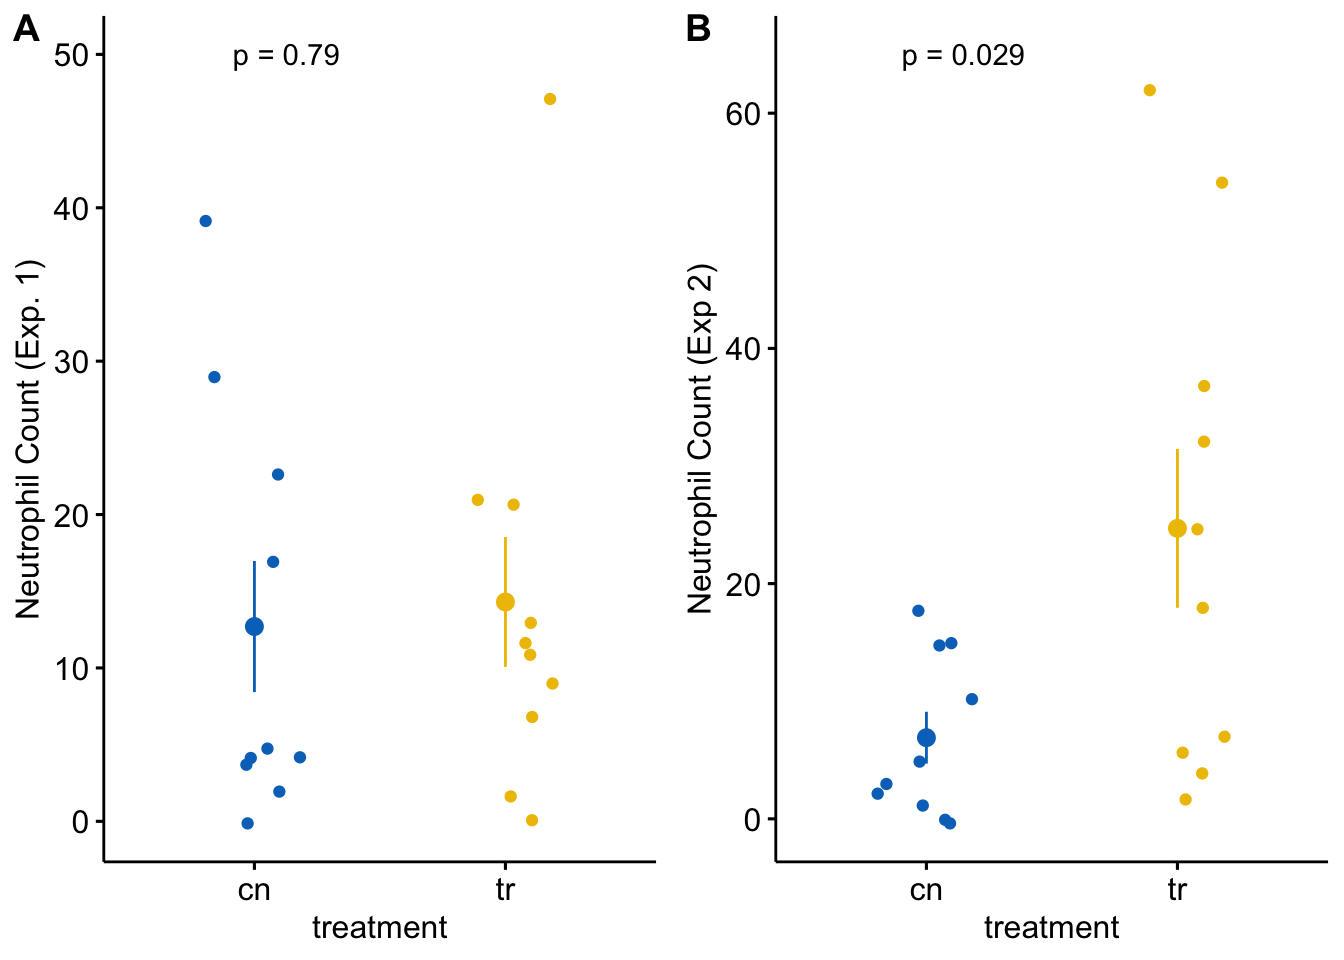
\includegraphics{Walker-elementary-statistical-modeling-draft_files/figure-latex/intro-plot-1.pdf}

\hypertarget{knit}{%
\subsection{Knit}\label{knit}}

\begin{enumerate}
\def\labelenumi{\arabic{enumi}.}
\setcounter{enumi}{5}
\tightlist
\item
  Knit to an html file
\item
  Knit to a pdf file
\item
  Knit to a word document
\end{enumerate}

Add the code option \texttt{echo\ =\ FALSE} to each chunk and re-knit to html, pdf, and word

\hypertarget{data-reading-wrangling-and-writing}{%
\chapter{Data -- Reading, Wrangling, and Writing}\label{data-reading-wrangling-and-writing}}

Importing data into R can be a struggle for new R users and, unfortunately, most online ``how to import'' sources give easy but superficial methods that don't follow best practices for increasing reproducibility or do not allow flexible organization of files within a project. Go straight to (Working in R){[}data-working-in-r{]} if you just want to learn the method used to import files in this text and don't care about important background information.

Some examples:

\begin{enumerate}
\def\labelenumi{\arabic{enumi}.}
\tightlist
\item
  \texttt{df\ \textless{}-\ read.table(file="clipboard")} imports data copied to the clipboard, from an Excel/Sheets file or from an open text file. For this to be semi-reproducible, a comment specifying the filename, worksheet and range that was copied is necessary. More problematic (catastrophically so for reproducibility), is, how does a researcher know that they highlighted and copied the correct range in the Excel sheet?
\item
  \texttt{df\ \textless{}-\ read.csv(file.choose())} opens the familiar ``open file'' dialog box, which lets the user navigate to the file of choice. For this to be semi-reproducible, a comment specifying the filename to import is necessary. The catastrophic problem (for reproducibility) is, how does a researcher know which file was actually opened during an R session? The researcher might think they opened ``walker\_maine\_bee\_data\_clean\_androscoggin.csv'' but mistakenly opened ``walker\_maine\_bee\_data\_clean\_aroostook.csv''.
\item
  \texttt{df\ \textless{}-\ read.table(file="my\_data.txt")} and \texttt{df\ \textless{}-\ read\_excel(file="my\_data.xlsx")} are reproducible because the filename is explicitly specified. But, this method requires that ``my\_data'' is physically located in the same folder as the file containing the R script (the notebook .Rmd file in our case) and this violates the best practice of clean project organization with different folders for the different kinds of files (data, R scripts, images, manuscript text, etc.).
\item
  R Studio has an elegant import tool in the environment pane that opens a custom dialog box that allows the researcher to navigate to the file, and to specify what part of the file to import, such as the specific sheet and range for an Excel file. This has the same reproducibility issues as \#1 and \#2 but R Studio includes the equivalent script, which adds all relevant information for reproducility. One then simply copies and pastes this script into a code chunk and voila! The next time the script is run, the data can be imported from the script without using menus and dialog boxes. Except that..the script does not seem to take into account that the \textbf{working directory} of an R Markdown file is not the project folder but the folder containing the R Markdown file and so this two-step method fails. More personally, I'd prefer to run a chunk that quickly opens the data file instead of re-navigating through my file system and re-specifying the sheet and range every time I re-start the project in a new R session.
\end{enumerate}

There are at least three solutions to the issues raised above, all requiring some understanding of \textbf{file paths} and directory structure in an operating system. A file such as ``my\_data.xlsx'' has an \textbf{absolute} file path, which is the full address of the file (the filename is something like your house street number). The absolute file path of ``my\_data.xlsx'' might be ``/Users/jwalker/Documents/applied-biostatistics/data/my\_data.xlsx''. A \textbf{relative} file path is the file path from the \textbf{working directory}. In an R Studio project, the working directory is the project directory, which is the directory containing the .Rproj file. This will be the working directory of the console. \emph{Importantly}, the working directory of an R Markdown code chunk is the folder containing the saved R Markdown file. An R Studio Notebook is an R Markdown file so the working directory of a notebook code chunk is the folder containing the saved notebook file. If a notebook file is located within the notebooks folder, which is located within the project folder, then the relative file path to ``my\_file.xlsx'' is ``../data/my\_file.xlsx''. The ``..'' tells the file OS to move ``up'' into the parent directory (which is the project folder) and the ``data'' tells the file OS to move ``down'' into the data folder. These are put together into a single address using ``/''. The beauty of relative paths is that they remain the same -- and so do not break one's script -- if the project folder, and all of its contents including the data folder and the notebooks folder, is moved to another location on the hard drive (say into a new ``Research'' folder). By contrast, the absolute file path changes, which breaks any old script.

The three solutions are

\begin{enumerate}
\def\labelenumi{\arabic{enumi}.}
\tightlist
\item
  Create a \textbf{relative path} to the file using something like \texttt{file\_path\ \textless{}-\ "../data/my\_data.xlsx"}. This should \emph{always} work but it fails on some computers. For example, if the project folder is on a Windows OS (but not Mac OS) desktop, the assigned relative address doesn't seem to look in the folder containing the file.
\item
  Create a setup chunk that reroutes the working directory to the project folder using the script
\end{enumerate}

\begin{Shaded}
\begin{Highlighting}[]
\CommentTok{# use this in a chuck called "setup" to force the working directory to be}
\CommentTok{# at the level of the project file.}
\NormalTok{knitr}\OperatorTok{::}\NormalTok{opts_knit}\OperatorTok{$}\KeywordTok{set}\NormalTok{(}\DataTypeTok{root.dir =}\NormalTok{ rprojroot}\OperatorTok{::}\KeywordTok{find_rstudio_root_file}\NormalTok{())}
\end{Highlighting}
\end{Shaded}

For this to work, the chunk has to be named ``setup'', that is, the text inside the curly brackets at the top of the chunk should be ``r setup''. Then, with this chunk, the relative file path is \texttt{file\_path\ \textless{}-\ "../data/my\_data.xlsx"} if ``my\_data.xlsx'' is immediately inside the data folder which is immediately inside the project folder. This should work on any machine, and should work even if a project folder is moved.

\begin{enumerate}
\def\labelenumi{\arabic{enumi}.}
\setcounter{enumi}{2}
\tightlist
\item
  Use the function here(). The most robust solution seems to be using the function here() from the here package. The function works something like this
\end{enumerate}

\begin{Shaded}
\begin{Highlighting}[]
\NormalTok{data_folder <-}\StringTok{ "data"} \CommentTok{# path to data that are imported}
\NormalTok{file_name <-}\StringTok{ "my_data.xlsx"}
\NormalTok{file_path <-}\StringTok{ }\KeywordTok{here}\NormalTok{(data_folder, file_name) }\CommentTok{# paste together parts of the address}
\NormalTok{my_file <-}\StringTok{ }\KeywordTok{read_excel}\NormalTok{(}\DataTypeTok{file =}\NormalTok{ file_path)}
\end{Highlighting}
\end{Shaded}

\texttt{here()} creates an absolute path, but one that is created on the fly, and will change (or should change) correctly if the project folder is moved on the same machine or to another machine.

\hypertarget{learning-from-this-chapter}{%
\section{Learning from this chapter}\label{learning-from-this-chapter}}

It will be easiest to learn from this chapter by starting with a clean notebook for the chapter. Create a new notebook and save it to the ``notebooks'' folder of your ``applied biostats'' project. \textbf{Important:} import/export scripts will not work properly until the file is saved! Get in the habit of creating the file, saving it immediately, and saving it often.

\begin{enumerate}
\def\labelenumi{\arabic{enumi}.}
\tightlist
\item
  Delete everything after the YAML header (this is the section at the top bounded by the ``---''.
\item
  Create a setup chunk that loads packages and creates variables for the locations of reading, writing, and image folders.
\end{enumerate}

\begin{Shaded}
\begin{Highlighting}[]
\CommentTok{# import and wrangling packages}
\KeywordTok{library}\NormalTok{(here) }\CommentTok{# here() creates the absolute path to the file}
\KeywordTok{library}\NormalTok{(janitor) }\CommentTok{# clean_names to clean col labels of imported data}
\KeywordTok{library}\NormalTok{(readxl) }\CommentTok{# import excel}
\KeywordTok{library}\NormalTok{(data.table) }\CommentTok{# use data.table for wrangling}

\CommentTok{# analysis packages}
\KeywordTok{library}\NormalTok{(emmeans) }\CommentTok{# get estimated marginal means and CIs, used for plot}

\CommentTok{# plotting packages}
\KeywordTok{library}\NormalTok{(ggplot2) }\CommentTok{# ggplot environment}
\KeywordTok{library}\NormalTok{(ggpubr) }\CommentTok{# publication ready plots}

\NormalTok{here <-}\StringTok{ }\NormalTok{here}\OperatorTok{::}\NormalTok{here }\CommentTok{# make sure ``here` uses `here::here`}

\CommentTok{# relative paths to project folders}
\NormalTok{data_folder <-}\StringTok{ "data"} \CommentTok{# path to data that are imported}
\NormalTok{output_folder <-}\StringTok{ "output"} \CommentTok{# path to data that are saved}
\NormalTok{image_folder <-}\StringTok{ "images"}
\end{Highlighting}
\end{Shaded}

Note on the script above
1. Be kind to the future you by loading only the packages necessary for the code in the R Markdown file that you are working on. If your default is to load everything, the future you will be confused why something was installed.
2. Be kind to the future you by commenting on why a package is loaded; usually this is a specific function from the package
3. \texttt{here\ \textless{}-\ here::here} is my favorite script ever. What is it doing? One can read this as ``assign the function here from the here package to the object here'' (this is reading the script right to left). Why do this? It turns out the multiple packages define a function called ``here''. If any of these packages are loaded after the here package, then \texttt{here} from here won't work -- it will be replaced by \texttt{here} from the more recently loaded package. To make sure that \texttt{here} uses the function from the here package, I simply reassign \texttt{here} from the here package to the object ``here'' \emph{after} loading in all packages.

\hypertarget{data-working-in-r}{%
\section{Working in R}\label{data-working-in-r}}

\hypertarget{importing-data}{%
\subsection{Importing data}\label{importing-data}}

\hypertarget{excel-file}{%
\subsubsection{Excel file}\label{excel-file}}

The Excel dataset is from an experiment on the growth response of zebra finch chicks to an incubation call that presumably signals ``hot environment'' to the embryos (\href{http://science.sciencemag.org/content/353/6301/812}{Mariette, M.M. and Buchanan, K.L., 2016. Prenatal acoustic communication programs offspring for high posthatching temperatures in a songbird. Science, 353(6301), pp.812-814}). The source file is from the Dryad Repository here:

\textbf{file name}: ``allDatasetsMarietteBuchanan2016.xls''

\textbf{source}: \url{https://datadryad.org//handle/10255/dryad.122315}

Steps

\begin{enumerate}
\def\labelenumi{\arabic{enumi}.}
\tightlist
\item
  Copy the title of the article, which is ``Prenatal acoustic communication programs offspring for high post-hatching temperatures in a songbird''
\item
  Create a new folder within the ``data'' folder. Name the folder the title of the paper by pasting the name from the clipboard. This is the ``data from'' folder, since it contains the data from the publication with the title of the folder.
\item
  Download the .xls file into this folder
\end{enumerate}

A .xls file is an old (pre 2007) Microsoft Excel file type. It is a binary file and can only be opened into a readable format with software that knows how to translate the proprietary format. The more modern Excel file type is .xlsx, which contains within it multiple xml components. An xml file is a text file, and so contains readable content, but the content is xml code to display something. In general, I am a big advocate of archiving stuff as text files (manuscripts, data, scripts, blog posts) because these will \emph{always} be readable by future software. Microsoft Excel is not likely to die anytime soon and software that can read .xls and especially .xlsx files (again, .xlsx files are text files) is even less likely to disappear but we can feel even more confident if data are archived as text files. That said, a single microsoft excel file with multiple sheets is an efficient method for distributing data and the readxl package provides excellent tools for reading different sheets of a single .xls or .xlsx file.

The code below uses the function \texttt{read\_excel()} from the package readxl. More about the amazing power of this package is the \href{https://readxl.tidyverse.org}{tidyverse page} and \href{http://r4ds.had.co.nz/data-import.html}{chapter 11} in the \emph{R for Data Science} book.

\begin{Shaded}
\begin{Highlighting}[]
\NormalTok{folder <-}\StringTok{ "Prenatal acoustic communication programs offspring for high post-hatching temperatures in a songbird"}
\NormalTok{fn <-}\StringTok{ "allDatasetsMarietteBuchanan2016.xls"}
\NormalTok{file_path <-}\StringTok{ }\KeywordTok{here}\NormalTok{(data_folder, folder, fn)}
\NormalTok{chick <-}\StringTok{ }\KeywordTok{read_excel}\NormalTok{(file_path, }
                    \DataTypeTok{sheet =} \StringTok{"nestlingMass"}\NormalTok{) }\OperatorTok\StringTok{ }\CommentTok{# import}
\StringTok{  }\KeywordTok{clean_names}\NormalTok{() }\OperatorTok\StringTok{ }\CommentTok{# clean the column names}
\StringTok{  }\KeywordTok{data.table}\NormalTok{() }\CommentTok{# convert to data.table}
\end{Highlighting}
\end{Shaded}

This text will consistently uses this protocol for storing and retrieving downloaded files. The first three lines in the script above creates the directory path to the file. This path includes three variables

\begin{enumerate}
\def\labelenumi{\arabic{enumi}.}
\tightlist
\item
  \texttt{data\_folder} -- assigned to ``data'' in the setup chunk. ``data'' is a folder within the project folder that contains (or will contain) all datasets for this text. The data come from many different published papers, so the data for each publication gets its own folder within ``data''.
\item
  \texttt{folder} -- the name of the ``data from'' folder within ``data'' containing the data files. In this text, these folder names will always be the name of the published paper.
\item
  \texttt{filename} -- the name of the file to read. There may be multiple data files within the publication's data folder.
\end{enumerate}

These are all put together into the absolute path using the function \texttt{here()} from the here package. Take a look at the value of file\_path to confirm.

The last four lines (starting with \texttt{chick\ \textless{}-}) contains three functions that are \textbf{piped} together using the pipe operator \texttt{\%\textgreater{}\%}. These functions

\begin{enumerate}
\def\labelenumi{\arabic{enumi}.}
\tightlist
\item
  read the specified data from the specified file and assign this to \texttt{chick}
\item
  clean the column names of the data.frame
\item
  convert the data.frame to a data.table.
\end{enumerate}

There are multiple ways to do this exactly this, including

A copy of the code above, which uses pipes

\begin{Shaded}
\begin{Highlighting}[]
\NormalTok{chick <-}\StringTok{ }\KeywordTok{read_excel}\NormalTok{(file_path, }
                    \DataTypeTok{sheet =} \StringTok{"nestlingMass"}\NormalTok{) }\OperatorTok\StringTok{ }\CommentTok{# import}
\StringTok{  }\KeywordTok{clean_names}\NormalTok{() }\OperatorTok\StringTok{ }\CommentTok{# clean the column names}
\StringTok{  }\KeywordTok{data.table}\NormalTok{() }\CommentTok{# convert to data.table}
\end{Highlighting}
\end{Shaded}

Very similar to the code above but without pipes. This requires complete assignment statements (\texttt{meh\ \textless{}-\ blah}). This is easy to read but the pipes (above) use slightly less type and indent the post-import-processing steps and so the pipes make the script a wee bit more organized.

\begin{Shaded}
\begin{Highlighting}[]
\NormalTok{chick <-}\StringTok{ }\KeywordTok{read_excel}\NormalTok{(file_path, }
                    \DataTypeTok{sheet =} \StringTok{"nestlingMass"}\NormalTok{)}\CommentTok{# import}
\NormalTok{chick <-}\StringTok{ }\KeywordTok{clean_names}\NormalTok{(chick) }\CommentTok{# clean the column names}
\NormalTok{chick <-}\StringTok{ }\KeywordTok{data.table}\NormalTok{(chick) }\CommentTok{# convert to data.table}
\end{Highlighting}
\end{Shaded}

The script above that simply embeds each function. To read this, you have to start deep and then move out. This is easy enough for this statement if you are used to reading this kinda stuff. But nests of embedded functions can quickly become hard to read and the future you will be happy if you don't do this. I sometimes will nest a single function in another but I'm trying to switch my default to pipes.

\begin{Shaded}
\begin{Highlighting}[]
\NormalTok{chick <-}\StringTok{ }\KeywordTok{data.table}\NormalTok{(}\KeywordTok{clean_names}\NormalTok{(}\KeywordTok{read_excel}\NormalTok{(file_path, }
                    \DataTypeTok{sheet =} \StringTok{"nestlingMass"}\NormalTok{))) }\CommentTok{# convert to data.table}
\end{Highlighting}
\end{Shaded}

\hypertarget{the-read_excel-function}{%
\paragraph{The read\_excel function}\label{the-read_excel-function}}

\texttt{read\_excel} is a beautifully flexible function because Excel. Data can be in different sheets and there can be different datasets within a single sheet. And, researchers tend to use Excel like a blackboard in that an Excel sheet often contains calculations such as means, standard deviations and t-tests. When using \texttt{read\_excel} it is important to send the function enough information to read the correct data. For the chick data, if we simply used

\begin{Shaded}
\begin{Highlighting}[]
\NormalTok{chick <-}\StringTok{ }\KeywordTok{read_excel}\NormalTok{(file_path) }\OperatorTok
\StringTok{  }\KeywordTok{clean_names}\NormalTok{() }\OperatorTok
\StringTok{  }\KeywordTok{data.table}\NormalTok{()}
\end{Highlighting}
\end{Shaded}

without specifying the sheet, \texttt{read\_excel} defaults to reading the first sheet (``OccurrenceIncubationCall''), which is not what we wanted. We can specify the exact range to important using the \texttt{range\ =} argument

\begin{Shaded}
\begin{Highlighting}[]
\NormalTok{chick <-}\StringTok{ }\KeywordTok{read_excel}\NormalTok{(file_path, }
                    \DataTypeTok{sheet =} \StringTok{"nestlingMass"}\NormalTok{,}
                    \DataTypeTok{range =} \StringTok{"A1:Q131"}\NormalTok{) }\OperatorTok\StringTok{ }\CommentTok{# import}
\StringTok{  }\KeywordTok{clean_names}\NormalTok{() }\OperatorTok\StringTok{ }\CommentTok{# clean the column names}
\StringTok{  }\KeywordTok{data.table}\NormalTok{() }\CommentTok{# convert to data.table}
\end{Highlighting}
\end{Shaded}

This isn't necessary for these data because the ``nestlingMass'' sheet contains only a matrix of data and not extraneous information and the \texttt{read\_excel} function is smart enough to figure this out. For many of the data sets in wet bench experimental biology, the range argument will be crucial.

\hypertarget{view-the-imported-data.table-to-check-that-the-file-was-imported-correctly-and-to-learn-about-the-contents.}{%
\paragraph{View the imported data.table to check that the file was imported correctly and to learn about the contents.}\label{view-the-imported-data.table-to-check-that-the-file-was-imported-correctly-and-to-learn-about-the-contents.}}

Insert the following after your import script and run:

\begin{Shaded}
\begin{Highlighting}[]
\KeywordTok{View}\NormalTok{(chick) }\CommentTok{# check}
\end{Highlighting}
\end{Shaded}

The line \texttt{View(chick)} script opens a new tab containing a spreadsheet-like display of the data.table \texttt{chick}.

Okay, let's back up to understand why we post-process with \texttt{clean\_names}. Re-import the data but without this function. I've done this by simply commenting out the line. The pipe above then skips over this and goes to \texttt{data.table()}.

\begin{Shaded}
\begin{Highlighting}[]
\NormalTok{chick <-}\StringTok{ }\KeywordTok{read_excel}\NormalTok{(file_path, }
                    \DataTypeTok{sheet=}\StringTok{"nestlingMass"}\NormalTok{) }\OperatorTok\StringTok{ }\CommentTok{# import}
\CommentTok{#  clean_names() %>% # clean the column names}
\StringTok{  }\KeywordTok{data.table}\NormalTok{() }\CommentTok{# convert to data.table}
\end{Highlighting}
\end{Shaded}

You can see the column names of \texttt{chick} using View but I find it easier to look at these names using \texttt{names} or \texttt{colnames} (yes, there are elebenty million ways to do anything in R) (\texttt{names} is very general in that it can be used to return the names of the parts of any list, while \texttt{colnames} is specific to matrix-like objects)

\begin{Shaded}
\begin{Highlighting}[]
\KeywordTok{names}\NormalTok{(chick)}
\end{Highlighting}
\end{Shaded}

\begin{verbatim}
##  [1] "chick ID"                       "brood ID"                      
##  [3] "brood composition"              "sex"                           
##  [5] "rank in nest"                   "playback treatment"            
##  [7] "nest temperature above ambient" "max daily temp hatch day"      
##  [9] "mean max temp hatch to day2"    "mean max temp hatch to day10"  
## [11] "mean max temp hatch to day13"   "hatching mass"                 
## [13] "day1 mass"                      "day2 mass"                     
## [15] "day10 mass"                     "day13 mass"                    
## [17] "day13 tarsus"
\end{verbatim}

In general, it is bad practice to include spaces, parentheses, and special characters such as -, \$ or \^{}, in the column names of a data frame because these increase handling costs later on. The best practice is to replace a blank with an underscore, for example \texttt{rank\_in\_nest}. Some coders separate words with a period (\texttt{rank.in.nest}). Others mash words together into a single word like this \texttt{rankinnest} but this should generally be avoided because the result can be hard to read. Finally, some coders use Caps to separate words like this \texttt{RankInNest}. This is easier to read than simple concatenation but the underscore is the easiest to read.

The \texttt{clean\_names} from the janitor package is a beautiful function to clean the column names of a data frame including replacing spaces with an underscore and stripping parentheses. The default clean includes changing any uppercase letter to lower case. Many coders like to work with all lowercase variable names to avoid having to hit the shift key. I am one of these.

\textbf{Worst Practices} -- resist the temptation to change the column names in the data file, which reduces reproducibility. Leave original data files original. Always increase reproducibility!

\textbf{colleague blues} -- Most researchers live in an Excel world and save data in a way that is efficient for computing stuff in Excel but not efficient for statistical analysis using R or other statistical computing software packages (with the exception of Graphpad Prism). Analyzing data will be much less frustrating if the data are saved in a format that facilitates analysis. Best practices for creating data files

\begin{enumerate}
\def\labelenumi{\arabic{enumi}.}
\item
  \url{https://www.youtube.com/watch?time_continue=309\&v=Ry2xjTBtNFE} -- An excellent video introduction to best practices for organizing data in a spreadsheet that will subsequently be analyzed by statistics software.
\item
  Broman, K. W., \& Woo, K. H. (2017). Data organization in spreadsheets (No.~e3183v1). \url{https://doi.org/10.7287/peerj.preprints.3183v1} -- An excelllent review of best practices for organizing data in a spreadsheet.
\end{enumerate}

\textbf{beginner blues} -- after running the code with the clean\_names commented out, type this into the console \texttt{chick\ \textless{}-\ clean\_names(chick)}. Now if you look at the column names with \texttt{names(chick)}, you see the names have been cleaned. But, if you quit R Studio, then re-open the notebook and run the chunks, your column names will not be clean because your command to clean the names was not in the saved script but simply entered into the console. The memory of this change was lost when you quit R Studio. This is a very common beginner mistake -- make changes with scripts in the console that aren't preserved in the saved chunks in the notbook. I'm not advising against changing the values of objects in the console -- I do this frequently when debugging or to experiment -- but to simply be aware that if you want specific operations to be reproducible, they need to be in the saved chunks in your notebook file.

Delete the comment and re-run the chunk so that \texttt{chick} has clean names. Save the file!

\hypertarget{explore-with-plots}{%
\paragraph{Explore with plots}\label{explore-with-plots}}

Did I mention to delete the comment in front of \texttt{clean\_names} and re-run the chunk so that \texttt{chick} has clean names?

Just for fun, let's plot the data and reproduce something close to Fig. 2A and B. We are using the \texttt{qplot} function, which is from the ggplot2 package. qplots are quick plots -- something you want to do to quickly look at data but don't want to turn into a publication quality plot.

\begin{Shaded}
\begin{Highlighting}[]
\KeywordTok{qplot}\NormalTok{(}\DataTypeTok{x =}\NormalTok{ nest_temperature_above_ambient,}
      \DataTypeTok{y =}\NormalTok{ day13_mass,}
      \DataTypeTok{data =}\NormalTok{ chick[playback_treatment }\OperatorTok{==}\StringTok{ "treat"}\NormalTok{]) }\OperatorTok{+}
\StringTok{  }\KeywordTok{geom_smooth}\NormalTok{(}\DataTypeTok{method =} \StringTok{"lm"}\NormalTok{)}
\end{Highlighting}
\end{Shaded}

\begin{verbatim}
## `geom_smooth()` using formula 'y ~ x'
\end{verbatim}

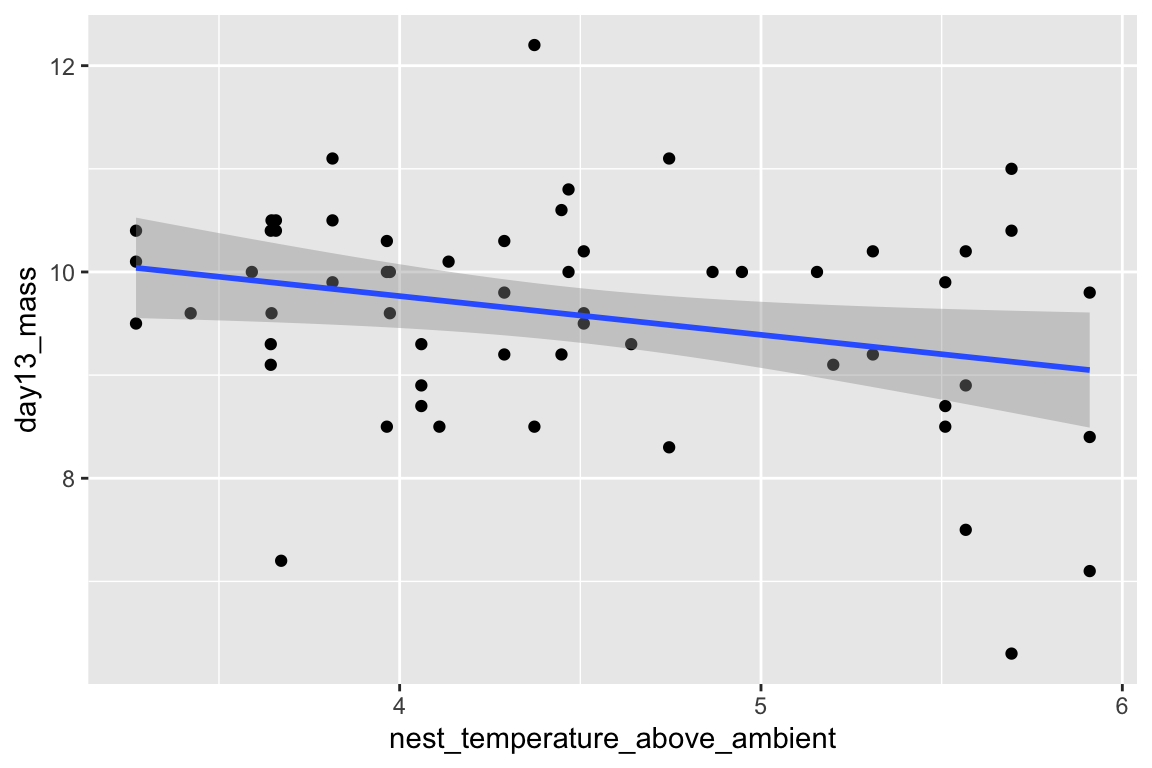
\includegraphics{Walker-elementary-statistical-modeling-draft_files/figure-latex/data-plotchickdata-1.pdf}

\begin{Shaded}
\begin{Highlighting}[]
\KeywordTok{qplot}\NormalTok{(}\DataTypeTok{x =}\NormalTok{ nest_temperature_above_ambient,}
      \DataTypeTok{y =}\NormalTok{ day13_mass,}
      \DataTypeTok{data =}\NormalTok{ chick[playback_treatment }\OperatorTok{==}\StringTok{ "cont"}\NormalTok{]) }\OperatorTok{+}
\StringTok{  }\KeywordTok{geom_smooth}\NormalTok{(}\DataTypeTok{method =} \StringTok{"lm"}\NormalTok{)}
\end{Highlighting}
\end{Shaded}

\begin{verbatim}
## `geom_smooth()` using formula 'y ~ x'
\end{verbatim}

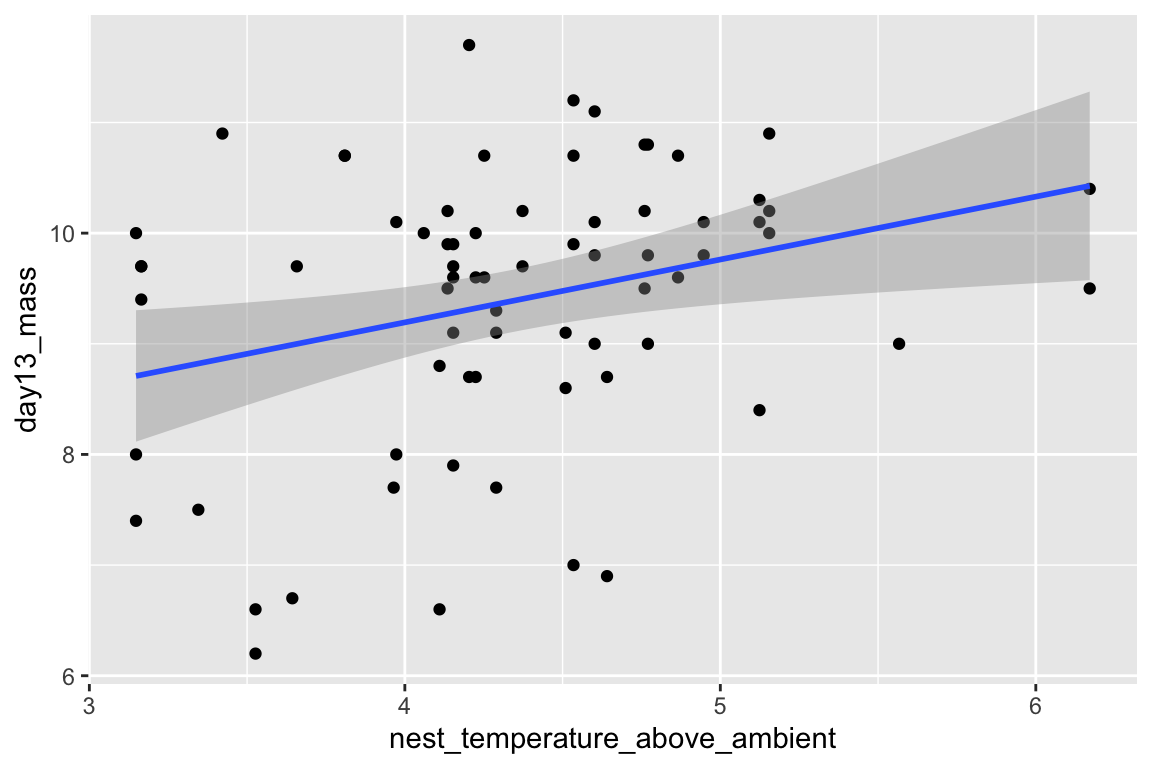
\includegraphics{Walker-elementary-statistical-modeling-draft_files/figure-latex/data-plotchickdata-2.pdf}

Notes on the code to make these plots

\begin{enumerate}
\def\labelenumi{\arabic{enumi}.}
\tightlist
\item
  the names of the columns to use as the x and y axes were not embedded into quotes (e.g.~``nest\_temperature\_above\_ambient''). Sometimes a column name has to be in quotes and sometimes not. In general, if the column name is sent to the function as a list (even if its a list with a single item), the names need to be in quotes. Regardless, remember this when you are debugging.
\item
  The first plot includes only the subset of data in which the value of \texttt{playback\_treatment} is ``treat''. Similarly, the second plot includes only the subset of data in which the value of \texttt{playback\_treatment} is ``cont''. I have sent a subset of the data to the plot function. There are elebenty million ways to subset data in R, I have done it the ``data.table way''.
\item
  each argument in the qplot function is on a separate line (created by adding a return after the comma) and the \texttt{geom\_smooth} function is on a new line. This just makes the function more readable then not doing this. What do you think?
\end{enumerate}

\begin{Shaded}
\begin{Highlighting}[]
\KeywordTok{qplot}\NormalTok{(}\DataTypeTok{x =}\NormalTok{ nest_temperature_above_ambient, }\DataTypeTok{y =}\NormalTok{ day13_mass, }\DataTypeTok{data =}\NormalTok{ chick[playback_treatment }\OperatorTok{==}\StringTok{ "treat"}\NormalTok{]) }\OperatorTok{+}\StringTok{ }\KeywordTok{geom_smooth}\NormalTok{(}\DataTypeTok{method =} \StringTok{"lm"}\NormalTok{)}
\end{Highlighting}
\end{Shaded}

\begin{enumerate}
\def\labelenumi{\arabic{enumi}.}
\setcounter{enumi}{3}
\tightlist
\item
  I have included the name of each argument. This isn't necessary but it makes the function more readable \emph{and} avoids potential bugs. The arguments without the argument names looks like this
\end{enumerate}

\begin{Shaded}
\begin{Highlighting}[]
\KeywordTok{qplot}\NormalTok{(nest_temperature_above_ambient, day13_mass, }\DataTypeTok{data =}\NormalTok{ chick[playback_treatment }\OperatorTok{==}\StringTok{ "treat"}\NormalTok{]) }\OperatorTok{+}\StringTok{ }\KeywordTok{geom_smooth}\NormalTok{(}\DataTypeTok{method =} \StringTok{"lm"}\NormalTok{)}
\end{Highlighting}
\end{Shaded}

\hypertarget{text-file}{%
\subsubsection{Text file}\label{text-file}}

The example dataset comes from an experiment on the effect of \href{http://science.sciencemag.org/content/early/2012/03/28/science.1215025}{neonicotinoid pesticides on bumble bee colony growth}.

\textbf{file name}: ``Whitehorn, O'Connor, Wackers, Goulson (2012) Data from `Neonicotinoid pesticide reduces bumblebee colony growth and queen production'.csv.csv''

\textbf{source}: \url{https://datadryad.org//resource/doi:10.5061/dryad.1805c973}

Steps

\begin{enumerate}
\def\labelenumi{\arabic{enumi}.}
\tightlist
\item
  Copy the title of the paper title, which is ``Neonicotinoid pesticide reduces bumblebee colony growth and queen production''
\item
  Create a new folder within ``data''. Name the folder the title of the paper by pasting from the clipboard. This is the ``data from'' folder, since it contains the data from the publication with the title of the folder.
\item
  Download the .csv file into this folder
\end{enumerate}

A .csv file is a text file that is comma-delimted, which means that the entries of a row are separated by commas. A text file is readable by any text editor software and most other kinds of software. Datasets that are stored as text files are typically saved as either .csv (where the entries of a row are separated by commas) or .txt (where the entries are separated by tabs). The base R way to read a .csv file is using \texttt{read.csv}. The \texttt{read.table} function is more versatile, as the delimiter can be specified. The function \texttt{fread()} from the data.table package is fast, smart, and flexible. It is smart in the sense that it guesses what the delimter is. Unfortunately, because of spaces in the column labels for this file, fread guesses incorrectly (another reason why spaces in column labels should be avoided). To overcome this, the statement below specifies that the file contains a ``header'' (a line containing column labels)

\begin{Shaded}
\begin{Highlighting}[]
\NormalTok{folder <-}\StringTok{ "Neonicotinoid pesticide reduces bumblebee colony growth and queen production"}
\NormalTok{filename <-}\StringTok{ "Whitehorn, O'Connor, Wackers, Goulson (2012) Data from 'Neonicotinoid pesticide reduces bumblebee colony growth and queen production'.csv.csv"}
\NormalTok{file_path <-}\StringTok{ }\KeywordTok{here}\NormalTok{(data_folder, folder, filename)}
\NormalTok{bee <-}\StringTok{ }\KeywordTok{fread}\NormalTok{(file_path, }\DataTypeTok{header=}\OtherTok{TRUE}\NormalTok{) }\OperatorTok
\StringTok{  }\KeywordTok{clean_names}\NormalTok{()}
\end{Highlighting}
\end{Shaded}

Here, as with the import of the Excel file, the first three lines create the directory path to the file. There is no need to pipe \texttt{bee} to \texttt{data.table()} because \texttt{fread} automatically importants the data as a data.table. It does not need to be converted.

Here is a reproduction of Fig 2 from the journal article.

\begin{Shaded}
\begin{Highlighting}[]
\NormalTok{bee[, treatment}\OperatorTok{:}\ErrorTok{=}\KeywordTok{factor}\NormalTok{(treatment, }\KeywordTok{c}\NormalTok{(}\StringTok{"Control"}\NormalTok{, }\StringTok{"Low"}\NormalTok{, }\StringTok{"High"}\NormalTok{))] }\CommentTok{# reorder factor levels}
\KeywordTok{ggbarplot}\NormalTok{(}\DataTypeTok{data=}\NormalTok{bee, }\DataTypeTok{x=}\StringTok{"treatment"}\NormalTok{, }\DataTypeTok{y=}\StringTok{"new_queens"}\NormalTok{, }\DataTypeTok{add =} \StringTok{"mean_se"}\NormalTok{)}
\end{Highlighting}
\end{Shaded}

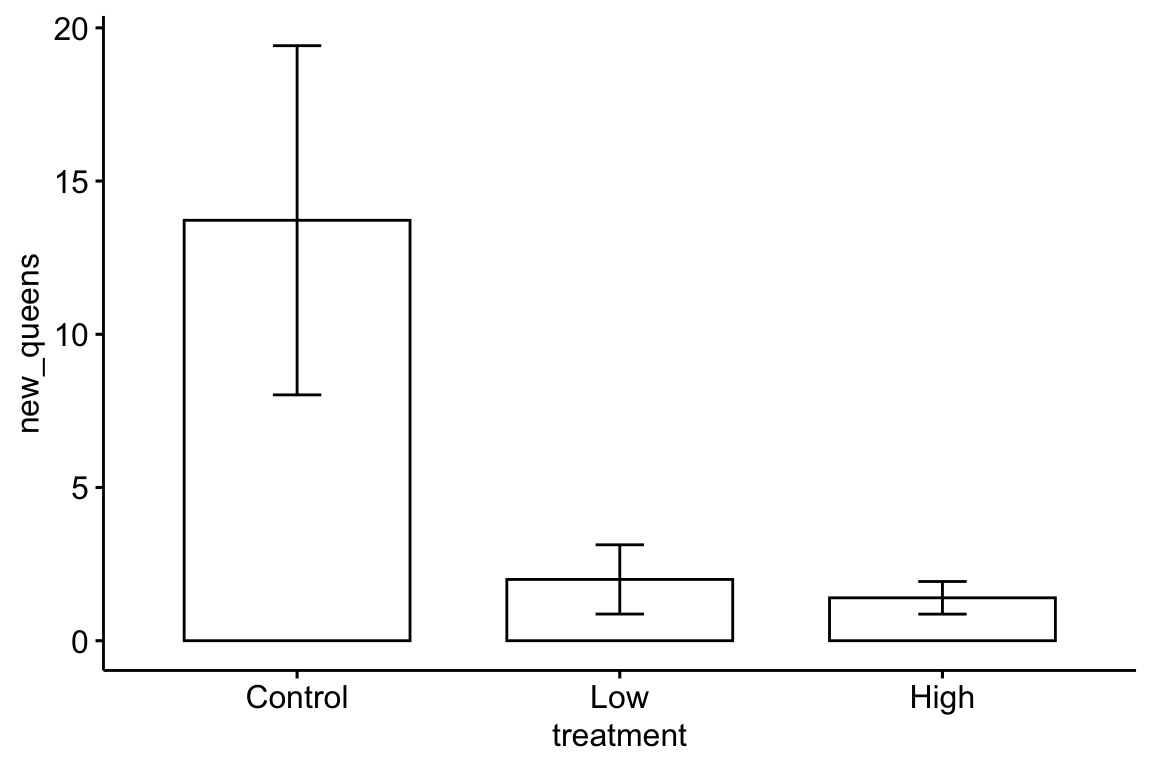
\includegraphics{Walker-elementary-statistical-modeling-draft_files/figure-latex/data-plot-bee-fig-2-1.pdf}

\hypertarget{troubleshooting-file-import}{%
\subsubsection{Troubleshooting file import}\label{troubleshooting-file-import}}

If you get an error that starts with ``Error: \texttt{path} does not exist:'' then R is not ``seeing'' your specified file given the path you've given it.

\begin{enumerate}
\def\labelenumi{\arabic{enumi}.}
\tightlist
\item
  Make sure you loaded the package \texttt{here} in a ``setup'' chunk and that you have run the chunk
\item
  Make sure you have assigned \texttt{data\_folder\ \textless{}-\ "data"} in the setup chunk and have run the chunk.
\item
  Make sure your ``data'' folder is \emph{one level} inside your project folder. ``one level'' means it is not buried deeper inside other folders within the project folder.
\item
  Make sure your ``data from'' folder (the folder with the title of the publication) is one level inside your ``data'' folder
\item
  Make sure your data file is one level inside the correct ``data from'' folder.
\item
  \textbf{Bug alert} Make sure you have the name of the ``data from \ldots{}'' folder correct in your script. Do not type the name of the folder. Instead, go to the finder and highlight the folder containing the data file, copy the name, return to the R markdown script, type \texttt{folder\ \textless{}-\ ""} and then paste the clipboard (the name of the folder) in between the quote marks.
\item
  \textbf{Bug alert} Make sure the file name is correct in the script. As with the folder name, I go to the finder and copy the file name and paste it in place. In Windows use ctrl-a instead of ctrl-c to copy the full filename including the extension.
\end{enumerate}

More generally, Humans are very good at understanding misspelled and OdDLy capitalized words but the R language (or any computer language) is very literal. R is \textbf{case sensitive} (some programming languages are not). ``Prenatal acoustic communication'', ``Prenatal Acoustic Communication'', and ``prenatal acoustic communication'' are all different values. Spelling AND capitalization have to be perfect, not simply close. Spelling includes \emph{spaces}. A frequent bug is a file name typed as ``Prenatal acoustic communication'' when the actual name is ``Prenatal acoustic communication''. Can you spot the bug? The original (what we need to copy) has two spaces between ``acoustic'' and ``communication'' while the incorrect copy has only one.

Spelling bugs are avoided by simply copying and pasting names of folders, names of files, column names of data frames, and level names of factors, which leads to a general rule of R scripting\ldots{}

\hypertarget{rule-number-one-in-r-scripting-rule1}{%
\subsubsection{Rule number one in R scripting \{\# rule1\}}\label{rule-number-one-in-r-scripting-rule1}}

\textbf{Always copy and paste any text that will be inserted into quotes}

Do not try to type it out. You have been warned.

\hypertarget{data-wrangling}{%
\section{Data wrangling}\label{data-wrangling}}

Data archived in Excel spreadsheets, at least in wet-bench experimental biology projects, are generally not in a format this is readily analyzed in R, or any statistical software other than perhaps Graphpad Prism. Use these examples as templates for how to import and wrangle Excel-archived data in your project.

\hypertarget{reshaping-data-wide-to-long}{%
\subsection{Reshaping data -- Wide to long}\label{reshaping-data-wide-to-long}}

\hypertarget{wide-to-long-adipsin-data}{%
\subsubsection{Wide to long -- Adipsin data}\label{wide-to-long-adipsin-data}}

Source: \href{https://www.nature.com/articles/s41591-019-0610-4}{Adipsin preserves beta cells in diabetic mice and associates with protection from type 2 diabetes in humans}

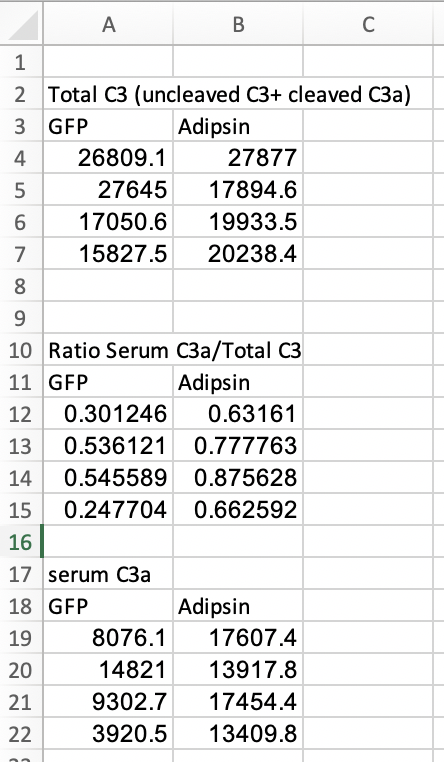
\includegraphics[width=0.6\linewidth]{/Users/jwalker/Documents/Github projects/Bookdown projects/applied-biostats/images/adipsin_fig1h_data}

Fig. 1h of the Adipsin paper presents three bar plots, each comparing a response variable between the control (GFP) and treated (Adipsin) groups. A screenshot of the Excel-archived data is shown above. The data are in \textbf{wide format}. In wide-format, the values of a variable are in separate columns for each treatment level (group). This is seen in the screenshot of the data. In the data for the first panel of Fig. 1h (Total C3), the values for the GFP group are in Column A and the values for the Adipsin group are in Column B. Wide format is efficient for computations in a spreadsheet, such as computing means and standard deviations of columns of data, and for plotting.

For most statistical analyses of experimental data in R (and most statistics software), all values of a single variable should be in a single column. This is called \textbf{long format}. I've rearranged the data from the archived spread sheet into long format by stacking each group's values into a single column, shown in the screen capture below. All values of total C3 are in a single column, as are the values for the other variables. In long format, there needs to be a way to identify which values belong to which group and this is achieved with column ``treatment''. In adition to the treatment column, I created a column containing the mouse identification number (I made these up as they were not given in the Excel-archived data).

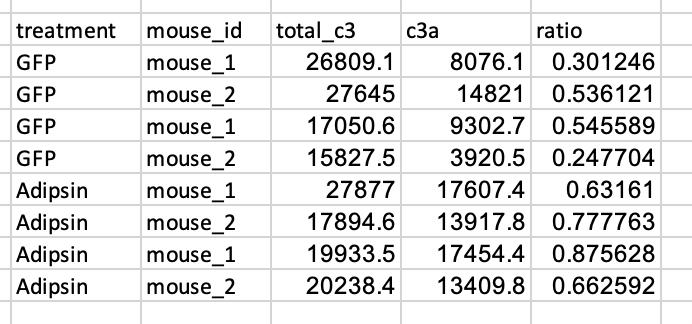
\includegraphics[width=0.6\linewidth]{/Users/jwalker/Documents/Github projects/Bookdown projects/applied-biostats/images/adipsin_fig1h_long}

The difference between wide and long also reflects how we think about statistical analysis. When we do a \emph{t}-test to compare the means of total C3 between GFP and Adipsin groups, we might think we have two things: the set of C3 values for the GFP group and the set of C3 values for the Adipsin group. When we fit a linear model, we also have two things, the variable \emph{treatment} containing treatment level assignment and the variable \emph{c3} containing the C3 values. In wide format, there is nothing to suggest that \emph{treatment} is a variable.

There are many functions to tidy data from wide to long. \texttt{melt} from the data.table package is especially useful. It is data.table's version of melt from the reshape2 package.

The major arguments of \texttt{data.table::melt} are

\texttt{melt(data,\ id.vars,\ measure.vars,\ variable.name,\ value.name)}

\texttt{melt} takes the data in the columns listed in \texttt{measure.vars} and stacks these into a single column named \texttt{value.name}. The names of the columns in \texttt{measure.vars} are the values of the elements in a new column named \texttt{variable.name}. The elements of any column in \texttt{id.vars} are repeated \emph{p} times, where \emph{p} is the number of columns that were stacked.

Let's melt the three different response variables of the adipsin data and \texttt{merge} them into a single data.table. There are several ways to combine data sets including \texttt{merge} and \texttt{cbind}. We'll compare these later.

\begin{Shaded}
\begin{Highlighting}[]
\NormalTok{file_folder <-}\StringTok{ "Adipsin preserves beta cells in diabetic mice and associates with protection from type 2 diabetes in humans"}
\NormalTok{fn <-}\StringTok{ "41591_2019_610_MOESM3_ESM.xlsx"}
\NormalTok{file_path <-}\StringTok{ }\KeywordTok{here}\NormalTok{(data_folder, file_folder, fn)}

\NormalTok{treatment_levels <-}\StringTok{ }\KeywordTok{c}\NormalTok{(}\StringTok{"GFP"}\NormalTok{,    }\StringTok{"Adipsin"}\NormalTok{)}

\CommentTok{# separately read each treatment}
\NormalTok{fig1h_total <-}\StringTok{ }\KeywordTok{read_excel}\NormalTok{(file_path,}
                    \DataTypeTok{sheet =} \StringTok{"Figure 1h"}\NormalTok{,}
                    \DataTypeTok{range =} \StringTok{"A3:B7"}\NormalTok{) }\OperatorTok
\StringTok{  }\KeywordTok{data.table}\NormalTok{() }\OperatorTok
\StringTok{  }\KeywordTok{melt}\NormalTok{(}\DataTypeTok{measure.vars =}\NormalTok{ treatment_levels,}
       \DataTypeTok{variable.name =} \StringTok{"treatment"}\NormalTok{,}
       \DataTypeTok{value.name =} \StringTok{"total_c3"}\NormalTok{)}
\CommentTok{# give each mouse a unique ID}
\NormalTok{fig1h_total[, mouse_id }\OperatorTok{:}\ErrorTok{=}\StringTok{ }\DecValTok{1}\OperatorTok{:}\NormalTok{.N]  }
  
\NormalTok{fig1h_ratio <-}\StringTok{ }\KeywordTok{read_excel}\NormalTok{(file_path,}
                    \DataTypeTok{sheet =} \StringTok{"Figure 1h"}\NormalTok{,}
                    \DataTypeTok{range =} \StringTok{"A11:B15"}\NormalTok{) }\OperatorTok
\StringTok{  }\KeywordTok{data.table}\NormalTok{() }\OperatorTok
\StringTok{  }\KeywordTok{melt}\NormalTok{(}\DataTypeTok{measure.vars =}\NormalTok{ treatment_levels,}
       \DataTypeTok{variable.name =} \StringTok{"treatment"}\NormalTok{,}
       \DataTypeTok{value.name =} \StringTok{"ratio"}\NormalTok{)}
\CommentTok{# give each mouse a unique ID}
\NormalTok{fig1h_ratio[, mouse_id }\OperatorTok{:}\ErrorTok{=}\StringTok{ }\DecValTok{1}\OperatorTok{:}\NormalTok{.N]  }

\NormalTok{fig1h_c3a <-}\StringTok{ }\KeywordTok{read_excel}\NormalTok{(file_path,}
                    \DataTypeTok{sheet =} \StringTok{"Figure 1h"}\NormalTok{,}
                    \DataTypeTok{range =} \StringTok{"A18:B22"}\NormalTok{) }\OperatorTok
\StringTok{  }\KeywordTok{data.table}\NormalTok{() }\OperatorTok
\StringTok{  }\KeywordTok{melt}\NormalTok{(}\DataTypeTok{measure.vars =}\NormalTok{ treatment_levels,}
       \DataTypeTok{variable.name =} \StringTok{"treatment"}\NormalTok{,}
       \DataTypeTok{value.name =} \StringTok{"c3a"}\NormalTok{)}
\CommentTok{# give each mouse a unique ID}
\NormalTok{fig1h_c3a[, mouse_id }\OperatorTok{:}\ErrorTok{=}\StringTok{ }\DecValTok{1}\OperatorTok{:}\NormalTok{.N] }

\NormalTok{fig1h <-}\StringTok{ }\KeywordTok{merge}\NormalTok{(fig1h_total, fig1h_c3a,}
               \DataTypeTok{by =} \KeywordTok{c}\NormalTok{(}\StringTok{"treatment"}\NormalTok{, }\StringTok{"mouse_id"}\NormalTok{))}
\NormalTok{fig1h <-}\StringTok{ }\KeywordTok{merge}\NormalTok{(fig1h, fig1h_ratio,}
               \DataTypeTok{by =} \KeywordTok{c}\NormalTok{(}\StringTok{"treatment"}\NormalTok{, }\StringTok{"mouse_id"}\NormalTok{))}
\NormalTok{fig1h[, check_ratio }\OperatorTok{:}\ErrorTok{=}\StringTok{ }\NormalTok{c3a}\OperatorTok{/}\NormalTok{total_c3]}

\CommentTok{# View(fig1h) # uncomment to view}
\NormalTok{fig1h}
\end{Highlighting}
\end{Shaded}

\begin{verbatim}
##    treatment mouse_id total_c3     c3a     ratio check_ratio
## 1:       GFP        1  26809.1  8076.1 0.3012458   0.3012447
## 2:       GFP        2  27645.0 14821.0 0.5361205   0.5361186
## 3:       GFP        3  17050.6  9302.7 0.5455894   0.5455937
## 4:       GFP        4  15827.5  3920.5 0.2477042   0.2477018
## 5:   Adipsin        5  27877.0 17607.4 0.6316098   0.6316103
## 6:   Adipsin        6  17894.6 13917.8 0.7777626   0.7777654
## 7:   Adipsin        7  19933.5 17454.4 0.8756279   0.8756315
## 8:   Adipsin        8  20238.4 13409.8 0.6625924   0.6625919
\end{verbatim}

\hypertarget{wide-to-long-enteric-nervous-system-data}{%
\subsubsection{Wide to long -- Enteric nervous system data}\label{wide-to-long-enteric-nervous-system-data}}

Article: Rolig, A. S., Mittge, E. K., Ganz, J., Troll, J. V., Melancon, E., Wiles, T. J., \ldots{} Guillemin, K. (2017). The enteric nervous system promotes intestinal health by constraining microbiota composition. PLOS Biology, 15(2), e2000689. \url{https://doi.org/10.1371/journal.pbio.2000689}

\textbf{Data source} \url{https://doi.org/10.1371/journal.pbio.2000689.s008}

\textbf{file name}: ``journal.pbio.2000689.s008.xlsx''

Let's import and reshape the data for figure 2d. Look at the excel file and the data in Fig. 2d. There is a single treament with four levels, but the authors have organized the data in each level in separate columns and used the column header as the level name.

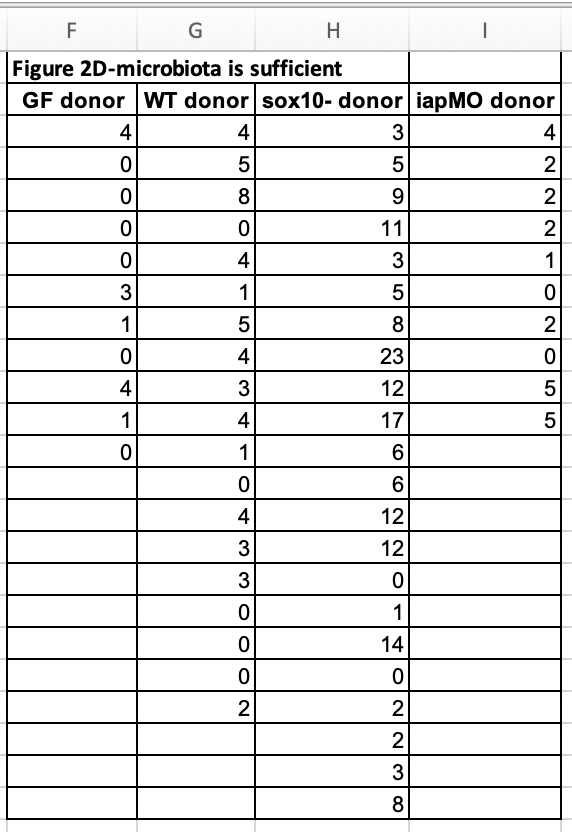
\includegraphics[width=0.6\linewidth]{/Users/jwalker/Documents/Github projects/Bookdown projects/applied-biostats/images/enteric_fig2d_wide}

Let's melt the data from wide to long by stacking the four columns into a single column ``neutrophil\_count'' and adding a treatment column identifying the group.

\begin{Shaded}
\begin{Highlighting}[]
\NormalTok{folder <-}\StringTok{ "The enteric nervous system promotes intestinal health by constraining microbiota composition"}
\NormalTok{filename <-}\StringTok{ "journal.pbio.2000689.s008.xlsx"}
\NormalTok{file_path <-}\StringTok{ }\KeywordTok{here}\NormalTok{(data_folder, folder, filename)}

\CommentTok{# figure 2D data}
\NormalTok{sheet_i <-}\StringTok{ "Figure 2"}
\NormalTok{range_i <-}\StringTok{ "F2:I24"}
\NormalTok{fig_2d_wide <-}\StringTok{ }\KeywordTok{read_excel}\NormalTok{(file_path, }\DataTypeTok{sheet=}\NormalTok{sheet_i, }\DataTypeTok{range=}\NormalTok{range_i) }\OperatorTok
\StringTok{  }\KeywordTok{clean_names}\NormalTok{() }\OperatorTok
\StringTok{  }\KeywordTok{data.table}\NormalTok{()}

\CommentTok{# change column names by replacing without "_donor" in each name}
\CommentTok{# these new column names will become the levels of the treatment factor}
\NormalTok{new_colnames <-}\StringTok{ }\KeywordTok{c}\NormalTok{(}\StringTok{"gf"}\NormalTok{, }\StringTok{"wt"}\NormalTok{, }\StringTok{"sox10"}\NormalTok{, }\StringTok{"iap_mo"}\NormalTok{)}
\KeywordTok{setnames}\NormalTok{(fig_2d_wide, }\DataTypeTok{old=}\KeywordTok{colnames}\NormalTok{(fig_2d_wide), }\DataTypeTok{new=}\NormalTok{new_colnames)}

\CommentTok{# wide to long}
\NormalTok{fig_2d <-}\StringTok{ }\KeywordTok{melt}\NormalTok{(fig_2d_wide, }
              \DataTypeTok{measure.vars=}\KeywordTok{colnames}\NormalTok{(fig_2d_wide), }
              \DataTypeTok{variable.name=}\StringTok{"treatment"}\NormalTok{, }
              \DataTypeTok{value.name=}\StringTok{"neutrophil_count"}\NormalTok{)}

\CommentTok{# omit empty rows}
\NormalTok{fig_2d <-}\StringTok{ }\KeywordTok{na.omit}\NormalTok{(fig_2d)}

\CommentTok{# re-order factors}
\NormalTok{fig_2d[, treatment }\OperatorTok{:}\ErrorTok{=}\StringTok{ }\KeywordTok{factor}\NormalTok{(treatment,}
                         \DataTypeTok{levels =} \KeywordTok{c}\NormalTok{(}\StringTok{"wt"}\NormalTok{, }\StringTok{"gf"}\NormalTok{, }\StringTok{"sox10"}\NormalTok{, }\StringTok{"iap_mo"}\NormalTok{))]}

\CommentTok{# View(fig_2d)}
\end{Highlighting}
\end{Shaded}

To learn (instead of just copy and modify), it's best to do this in steps and not run the whole chunk. At each step, look at the result using View. The script above includes three extra wrangling steps.

\begin{enumerate}
\def\labelenumi{\arabic{enumi}.}
\item
  Changing column names in fig\_2d\_wide. The column names in wide format will become the treatment level names of the \emph{treatment} factor after reshaping. It will be easier down the road if these names are shorter and the "\_donor" in each name is redundant. The \texttt{setnames} function renames the column names.
\item
  For these data, the number of measures within the different treatments differs and, as a consequence, there are multiple cells with \texttt{NA} which indicates a missing value. \texttt{View(fig\_2d\_wide)} (this can be typed in the console) to see this. After reshaping to long format (fig\_2d), the rows with missing values become empty rows -- there is no useful information in them (View this). To see this, re-run the lines of the chunk up to the line ``\# omit empty rows''. The \texttt{na.omit} function deletes any row with missing values. Here, this deletes these information-less rows. Be very careful with \texttt{na.omit}. You do not want to delete rows of data that contain information you want.
\item
  For both analysis and plots, we want to compare values to the control level, which is named ``wt'' for the fig\_2d data. That is, we want ``wt'' to be the \emph{reference} level. To achieve this, the levels of the factor \emph{treatment} need to be re-ordered using the \texttt{levels} argument. (note, I typically do not add ``levels ='', but simply pass the list of levels)
\end{enumerate}

\hypertarget{wide-to-long-bee-data}{%
\subsubsection{Wide to long -- bee data}\label{wide-to-long-bee-data}}

The example above is pretty easy, because the all columns in the original data frame are melted (stacked). Here is an example in which only a subset of columns are stacked. In addition, only a subset of the remaining columns are retained in the long format data frame. The data are from Panel A of supplement Fig. 8 (\url{https://journals.plos.org/plosbiology/article/file?type=supplementary\&id=info:doi/10.1371/journal.pbio.2003467.s019}) from

Kešnerová, L., Mars, R.A., Ellegaard, K.M., Troilo, M., Sauer, U. and Engel, P., 2017. Disentangling metabolic functions of bacteria in the honey bee gut. PLoS biology, 15(12), p.e2003467.

**data source*:** \url{https://doi.org/10.1371/journal.pbio.2003467.s001}

\begin{Shaded}
\begin{Highlighting}[]
\NormalTok{folder <-}\StringTok{ "Data from Disentangling metabolic functions of bacteria in the honey bee gut"}
\NormalTok{filename <-}\StringTok{ "journal.pbio.2003467.s001.xlsx"}

\CommentTok{# figure 2D data}
\NormalTok{sheet_i <-}\StringTok{ "S8 Fig"}
\NormalTok{range_i <-}\StringTok{ "A2:H12"}
\NormalTok{file_path <-}\StringTok{ }\KeywordTok{here}\NormalTok{(data_folder, folder, filename)}
\NormalTok{fig_s8a_wide <-}\StringTok{ }\KeywordTok{read_excel}\NormalTok{(file_path,}
                      \DataTypeTok{sheet=}\NormalTok{sheet_i,}
                      \DataTypeTok{range=}\NormalTok{range_i) }\OperatorTok
\StringTok{  }\KeywordTok{clean_names}\NormalTok{() }\OperatorTok
\StringTok{  }\KeywordTok{data.table}\NormalTok{()}

\CommentTok{# wide to long}
\NormalTok{stack_cols <-}\StringTok{ }\KeywordTok{paste0}\NormalTok{(}\StringTok{"replicate"}\NormalTok{, }\DecValTok{1}\OperatorTok{:}\DecValTok{5}\NormalTok{)}
\NormalTok{fig_s8a <-}\StringTok{ }\KeywordTok{melt}\NormalTok{(fig_s8a_wide,}
              \DataTypeTok{id.vars =} \KeywordTok{c}\NormalTok{(}\StringTok{"media"}\NormalTok{, }\StringTok{"time_h"}\NormalTok{),}
              \DataTypeTok{measure.vars =}\NormalTok{ stack_cols, }
              \DataTypeTok{variable.name =} \StringTok{"Replicate"}\NormalTok{, }
              \DataTypeTok{value.name =} \StringTok{"OD600"}\NormalTok{) }\CommentTok{# measure of absorbance at 600nm}
\end{Highlighting}
\end{Shaded}

\hypertarget{wide-to-long-stacking-multiple-sets-of-columns}{%
\subsubsection{Wide to long -- stacking multiple sets of columns}\label{wide-to-long-stacking-multiple-sets-of-columns}}

This example comes from my lab, where a student measured sprint speed in each fish three times prior to treatment and three times following treatment. The wide format data looked something like this

\begin{Shaded}
\begin{Highlighting}[]
\KeywordTok{set.seed}\NormalTok{(}\DecValTok{1}\NormalTok{)}
\NormalTok{fd_wide <-}\StringTok{ }\KeywordTok{data.table}\NormalTok{(}\DataTypeTok{fish_ID=}\KeywordTok{paste0}\NormalTok{(}\StringTok{"fish"}\NormalTok{,}\DecValTok{1}\OperatorTok{:}\DecValTok{4}\NormalTok{),}
                      \DataTypeTok{treatment=}\KeywordTok{rep}\NormalTok{(}\KeywordTok{c}\NormalTok{(}\StringTok{"cn"}\NormalTok{, }\StringTok{"tr"}\NormalTok{), }\DataTypeTok{each=}\DecValTok{2}\NormalTok{),}
                      \DataTypeTok{length=}\KeywordTok{rnorm}\NormalTok{(}\DecValTok{4}\NormalTok{, }\DecValTok{12}\NormalTok{, }\DecValTok{2}\NormalTok{),}
                      \DataTypeTok{pre_1=}\KeywordTok{rnorm}\NormalTok{(}\DecValTok{4}\NormalTok{, }\DecValTok{50}\NormalTok{, }\DecValTok{5}\NormalTok{),}
                      \DataTypeTok{pre_2=}\KeywordTok{rnorm}\NormalTok{(}\DecValTok{4}\NormalTok{, }\DecValTok{50}\NormalTok{, }\DecValTok{5}\NormalTok{),}
                      \DataTypeTok{pre_3=}\KeywordTok{rnorm}\NormalTok{(}\DecValTok{4}\NormalTok{, }\DecValTok{50}\NormalTok{, }\DecValTok{5}\NormalTok{),}
                      \DataTypeTok{post_1=}\KeywordTok{rnorm}\NormalTok{(}\DecValTok{4}\NormalTok{, }\DecValTok{50}\NormalTok{, }\DecValTok{5}\NormalTok{),}
                      \DataTypeTok{post_2=}\KeywordTok{rnorm}\NormalTok{(}\DecValTok{4}\NormalTok{, }\DecValTok{50}\NormalTok{, }\DecValTok{5}\NormalTok{),}
                      \DataTypeTok{post_3=}\KeywordTok{rnorm}\NormalTok{(}\DecValTok{4}\NormalTok{, }\DecValTok{50}\NormalTok{, }\DecValTok{5}\NormalTok{)}
\NormalTok{                      )}
\NormalTok{knitr}\OperatorTok{::}\KeywordTok{kable}\NormalTok{(fd_wide, }\DataTypeTok{digits=}\DecValTok{1}\NormalTok{)}
\end{Highlighting}
\end{Shaded}

fish\_ID

treatment

length

pre\_1

pre\_2

pre\_3

post\_1

post\_2

post\_3

fish1

cn

10.7

51.6

52.9

46.9

49.9

54.6

53.1

fish2

cn

12.4

45.9

48.5

38.9

54.7

53.9

49.7

fish3

tr

10.3

52.4

57.6

55.6

54.1

50.4

49.2

fish4

tr

15.2

53.7

51.9

49.8

53.0

40.1

42.6

To analyze the response (post-treatment sprint) adjusted for pre-treatment sprint, the three pre-treatment sprint measures need to be stacked into a single column and the three post-treatment measures need to be stacked into a single column. This is easy using \texttt{melt} from the data.table package.

\begin{Shaded}
\begin{Highlighting}[]
\NormalTok{pre_cols <-}\StringTok{ }\KeywordTok{paste}\NormalTok{(}\StringTok{"pre"}\NormalTok{, }\DecValTok{1}\OperatorTok{:}\DecValTok{3}\NormalTok{, }\DataTypeTok{sep=}\StringTok{"_"}\NormalTok{)}
\NormalTok{post_cols <-}\StringTok{ }\KeywordTok{paste}\NormalTok{(}\StringTok{"post"}\NormalTok{, }\DecValTok{1}\OperatorTok{:}\DecValTok{3}\NormalTok{, }\DataTypeTok{sep=}\StringTok{"_"}\NormalTok{)}
\NormalTok{fd <-}\StringTok{ }\KeywordTok{melt}\NormalTok{(fd_wide,}
           \DataTypeTok{id.vars=}\KeywordTok{c}\NormalTok{(}\StringTok{"fish_ID"}\NormalTok{, }\StringTok{"treatment"}\NormalTok{, }\StringTok{"length"}\NormalTok{),}
           \DataTypeTok{measure.vars=}\KeywordTok{list}\NormalTok{(pre_cols, post_cols),}
           \DataTypeTok{variable.name=}\StringTok{"Order"}\NormalTok{,}
           \DataTypeTok{value.name=}\KeywordTok{c}\NormalTok{(}\StringTok{"sprint_pre"}\NormalTok{, }\StringTok{"sprint_post"}\NormalTok{))}
\NormalTok{knitr}\OperatorTok{::}\KeywordTok{kable}\NormalTok{(fd, }\DataTypeTok{digits=}\DecValTok{1}\NormalTok{)}
\end{Highlighting}
\end{Shaded}

fish\_ID

treatment

length

Order

sprint\_pre

sprint\_post

fish1

cn

10.7

1

51.6

49.9

fish2

cn

12.4

1

45.9

54.7

fish3

tr

10.3

1

52.4

54.1

fish4

tr

15.2

1

53.7

53.0

fish1

cn

10.7

2

52.9

54.6

fish2

cn

12.4

2

48.5

53.9

fish3

tr

10.3

2

57.6

50.4

fish4

tr

15.2

2

51.9

40.1

fish1

cn

10.7

3

46.9

53.1

fish2

cn

12.4

3

38.9

49.7

fish3

tr

10.3

3

55.6

49.2

fish4

tr

15.2

3

49.8

42.6

\hypertarget{reshaping-data-transpose-turning-the-columns-into-rows}{%
\subsection{Reshaping data -- Transpose (turning the columns into rows)}\label{reshaping-data-transpose-turning-the-columns-into-rows}}

\hypertarget{transpose-pi3k-inhibitors-data}{%
\subsubsection{Transpose -- PI3K inhibitors data}\label{transpose-pi3k-inhibitors-data}}

Source: \href{https://www.nature.com/articles/s41586-018-0343-4}{Suppression of insulin feedback enhances the efficacy of PI3K inhibitors}

Figure 3A of this publication is a plot of blood glucose level taken on the same individual mice from four treatment groups over six time periods. Data on a single variable such as blood glucose, taken on the same individual at multiple time points, are known as \textbf{longitudial data} but are often mistakenly called \textbf{repeated measures data}. There are mulitple ways to analyze longitudinal data, some goood, some less good. There are two reasonable ways to archive longitudinal data for analysis in R. The Excel-archived data for Figure 3A is neither. A screen capture of two of the four treatment groups is shown below.

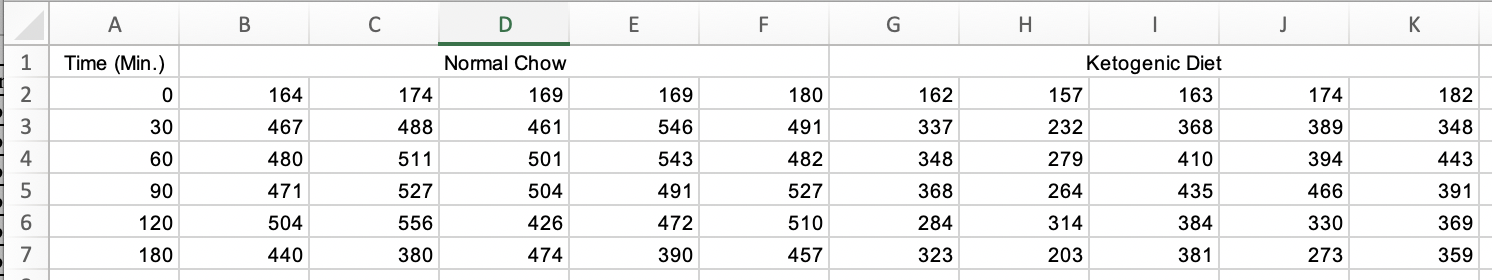
\includegraphics[width=0.6\linewidth]{/Users/jwalker/Documents/Github projects/Bookdown projects/applied-biostats/images/pi3k-inhibitors}

In the archived data the individual mice are in columns. The measure at each time point is in rows. And the treatment group is in blocks. Typical data for analysis in R should have the individual mice in rows and each variable in columns (an exception in experimental biology is omics data, such as RNA expression levels. Many packages with functions to analyze these data have the genes on each row and the individual on each column). The Figure 3A data are turned on its side. We need to \textbf{transpose} the data, or rotate the matrix 90 degrees (make the columns rows and the rows columns) to turn the data into wide format. From this we can create a new data.table with the data in long format.

\begin{Shaded}
\begin{Highlighting}[]
\NormalTok{folder <-}\StringTok{ "Suppression of insulin feedback enhances the efficacy of PI3K inhibitors"}
\NormalTok{filename <-}\StringTok{ "41586_2018_343_MOESM6_ESM.xlsx"}
\NormalTok{file_path <-}\StringTok{ }\KeywordTok{here}\NormalTok{(data_folder, folder, filename)}
\NormalTok{pi3k_side <-}\StringTok{ }\KeywordTok{read_excel}\NormalTok{(file_path,}
                    \DataTypeTok{sheet =} \StringTok{"Figure 3A (Blood Glucose)"}\NormalTok{,}
                    \DataTypeTok{range =} \StringTok{"A2:U7"}\NormalTok{,}
                    \DataTypeTok{col_names =} \OtherTok{FALSE}\NormalTok{) }\OperatorTok
\StringTok{  }\KeywordTok{data.table}\NormalTok{()}
\end{Highlighting}
\end{Shaded}

\begin{verbatim}
## New names:
## * `` -> ...1
## * `` -> ...2
## * `` -> ...3
## * `` -> ...4
## * `` -> ...5
## * ...
\end{verbatim}

\begin{Shaded}
\begin{Highlighting}[]
\CommentTok{# give columns names as the treatment of each mouse}
\CommentTok{# verify n=5 per group}
\NormalTok{treatment_levels <-}\StringTok{ }\KeywordTok{c}\NormalTok{(}\StringTok{"Chow"}\NormalTok{, }\StringTok{"Ketogenic"}\NormalTok{, }\StringTok{"Metformin"}\NormalTok{, }\StringTok{"SGLT2i"}\NormalTok{)}
\KeywordTok{colnames}\NormalTok{(pi3k_side) <-}\StringTok{ }\KeywordTok{c}\NormalTok{(}\StringTok{"time"}\NormalTok{,}
                         \KeywordTok{rep}\NormalTok{(treatment_levels, }\DataTypeTok{each =} \DecValTok{5}\NormalTok{))}

\CommentTok{# transpose}
\CommentTok{# keep colnames in "side" as values of treatment col in "wide"}
\CommentTok{# make values of "time" in "side" the colnames in "wide"}
\NormalTok{pi3k_wide <-}\StringTok{ }\KeywordTok{transpose}\NormalTok{(pi3k_side,}
                       \DataTypeTok{keep.names =} \StringTok{"treatment"}\NormalTok{, }
                       \DataTypeTok{make.names =} \StringTok{"time"}\NormalTok{)}

\CommentTok{# make a baseline column }
\NormalTok{pi3k_wide[, glucose_}\DecValTok{0} \OperatorTok{:}\ErrorTok{=}\StringTok{ }\KeywordTok{get}\NormalTok{(}\StringTok{"0"}\NormalTok{)]}

\CommentTok{# make-up a mouse id for each mouse}
\NormalTok{pi3k_wide[, id }\OperatorTok{:}\ErrorTok{=}\StringTok{ }\KeywordTok{paste}\NormalTok{(treatment, }\DecValTok{1}\OperatorTok{:}\NormalTok{.N, }\DataTypeTok{sep =} \StringTok{"_"}\NormalTok{), by =}\StringTok{ }\NormalTok{treatment]}

\CommentTok{# make treatement a factor with "chow" as reference}
\NormalTok{pi3k_wide[, treatment }\OperatorTok{:}\ErrorTok{=}\StringTok{ }\KeywordTok{factor}\NormalTok{(treatment, treatment_levels)]}

\CommentTok{# make a long version}
\NormalTok{pi3k_long <-}\StringTok{ }\KeywordTok{melt}\NormalTok{(pi3k_wide,}
                  \DataTypeTok{id.vars =} \KeywordTok{c}\NormalTok{(}\StringTok{"treatment"}\NormalTok{, }\StringTok{"id"}\NormalTok{, }\StringTok{"glucose_0"}\NormalTok{),}
                  \DataTypeTok{variable.name =} \StringTok{"time"}\NormalTok{,}
                  \DataTypeTok{value.name =} \StringTok{"glucose"}\NormalTok{)}
\end{Highlighting}
\end{Shaded}

Notes

\begin{enumerate}
\def\labelenumi{\arabic{enumi}.}
\tightlist
\item
  Read the comments on the usage of the \texttt{keep.names} and \texttt{make.names} arguments of \texttt{transpose}. These are powerful.
\item
  pi3k\_wide has column names that are times (in minutes). This presents wrangling problems (column names shouldn't be numbers. Here it is useful to create the long format data.table with a time column of numbers). For example, the code above creates copies the column ``0'' into a new column ``glucose\_0'' using \texttt{glucose\_0\ :=\ get("0")}. Had the code been \texttt{glucose\_0\ :=\ "0"}, all values would be the character ``0''. Had the code been \texttt{glucose\_0\ :=\ 0}, all values would be the number 0. \texttt{get} looks for the column with the name of whatever is inside the parentheses.
\end{enumerate}

Let's do a quick plot to examine the data

\begin{Shaded}
\begin{Highlighting}[]
\KeywordTok{qplot}\NormalTok{(}\DataTypeTok{x =}\NormalTok{ time,}
      \DataTypeTok{y =}\NormalTok{ glucose,}
      \DataTypeTok{data =}\NormalTok{ pi3k_long,}
      \DataTypeTok{color =}\NormalTok{ treatment) }\OperatorTok{+}
\StringTok{  }\KeywordTok{geom_line}\NormalTok{(}\KeywordTok{aes}\NormalTok{(}\DataTypeTok{group =}\NormalTok{ id))}
\end{Highlighting}
\end{Shaded}

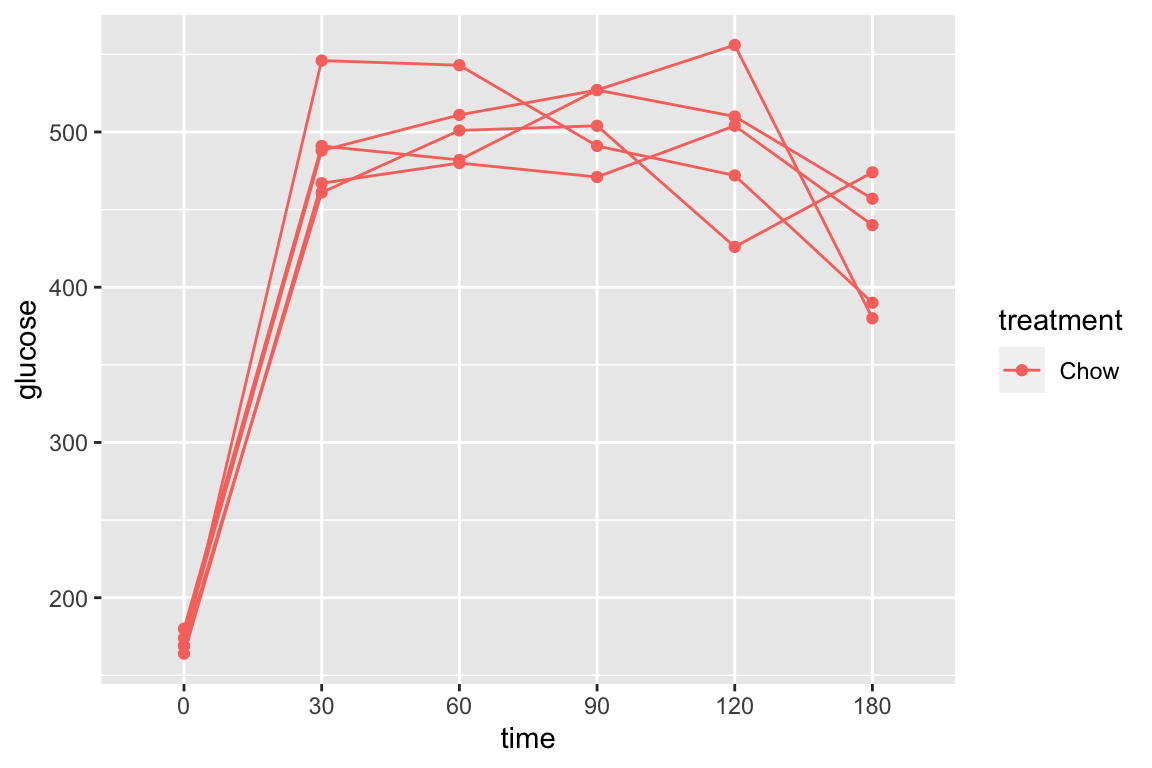
\includegraphics{Walker-elementary-statistical-modeling-draft_files/figure-latex/unnamed-chunk-61-1.pdf}

\hypertarget{combining-data}{%
\subsection{Combining data}\label{combining-data}}

\textbf{Source article} Bak, A.M., Vendelbo, M.H., Christensen, B., Viggers, R., Bibby, B.M., Rungby, J., Jørgensen, J.O.L., Møller, N. and Jessen, N., 2018. Prolonged fasting-induced metabolic signatures in human skeletal muscle of lean and obese men. PloS one, 13(9), p.e0200817.

\textbf{Data source} \url{https://datadryad.org/stash/dataset/doi:10.5061/dryad.6121hj7}

\textbf{file name}: datafiles.xlsx

The data are from a randomized \textbf{crossover} design where 18 men (9 lean and 9 obese) were measured for multiple metabolic markers at two times: 1) in a post-absorptive state after 12 hours overnight fast, and 2) in a prolonged fasting state after 72 hours of fasting. In addition, at each time point, metabolic markers were measured prior to and after an insulin infusion. Here, we want to reproduce values in Table 2, which are measures of mean blood insulin and metabolite levels after 12 hours and 72 hours fasting in both the lean and obese groups.

A difficulty for the analyst is that the response data are in the ``Table 2'' sheet but the variable containing the assignment to ``lean'' or ``obese'' group is in the ``Table 1'' sheet. To analyze these response, the two datasets need to be combined into a single data frame. The important consideration when combining data is that \emph{like is matched with like}. For the fasting dataset, ``like'' is the subject id, and we have some data for each subject id in Table 1 and other data for the same subject ids in Table 2. This means that we essentially want to glue the columns of table 2 to the columns of table 1 in a way that insures that the correct data for each subject id is on the same row. This is a bit more complicated for these data because Table 1 contains 18 data rows, one for each subject id and Table 2 contains 36 data rows, 2 for each subject id, because each subject has data measured at 12 hours and at 72 hours.

\hypertarget{subsetting-data}{%
\subsection{Subsetting data}\label{subsetting-data}}

It is common to see researchers create multiple subsets of data for further processing. This practice should be be discouraged because the same variables will be in multiple data frames and it can be hard to keep track of any processing of variables in the different datasets. Instead, subset the data at the level of analysis.

There are many ways to subset data in R. Experienced users tend to divide up into those using base R, those using the tidyverse packages, or those using data.table. Learn one well. This book uses data.table. Before outlining usage in data.table, let's back up a bit and review different \emph{indexing} systems.

\begin{itemize}
\tightlist
\item
  In Excel, rows are specified (or ``indexed'') by numbers and columns by letters. Every cell has an address, for example C2 is the cell in the 2nd row and 3rd column. Notice that in Excel, the column part of the address comes before the row part.
\item
  In statistics, it is extremely common to use a system where \(x_{ij}\) is the value of the element in the \emph{i}th row and \emph{j}th column of the matrix \textbf{X}. Notice that in this notatin, the row index (\emph{i}) comes before the column index (\emph{j}).
\item
  In programming languages, including R, it is extremely common to use a system where my\_data{[}i, j{]} is the value of the element in the \emph{i}th row and \emph{j}th column of the matrix-like object named ``my\_data'' (such as a data frame in R).
\item
  data.table explicitly refers to the row index and column index as \emph{i} and \emph{j}.
\end{itemize}

\hypertarget{specifying-a-subset-of-rows-observations-or-cases}{%
\subsubsection{Specifying a subset of rows (``observations'' or ``cases'')}\label{specifying-a-subset-of-rows-observations-or-cases}}

A subset of rows is specified using either a list of row numbers or

In a data.table, a subset of rows is specified using either a list of row numbers or a combination of comparison operators (==, !=, \textgreater, \textless, \textgreater=, \textless=, \%in\%) and Boolean logic operators (\&, \textbar, ! -- these are ``and'', ``or'', ``not'') as \emph{i}.

Let's use the pi3k\_long data from above to explore this. First, the plot of plasma glucose for all individuals in each treatment group across all time points.

\begin{Shaded}
\begin{Highlighting}[]
\KeywordTok{qplot}\NormalTok{(}\DataTypeTok{x =}\NormalTok{ time,}
      \DataTypeTok{y =}\NormalTok{ glucose,}
      \DataTypeTok{data =}\NormalTok{ pi3k_long,}
      \DataTypeTok{color =}\NormalTok{ treatment) }\OperatorTok{+}
\StringTok{  }\KeywordTok{geom_line}\NormalTok{(}\KeywordTok{aes}\NormalTok{(}\DataTypeTok{group =}\NormalTok{ id))}
\end{Highlighting}
\end{Shaded}

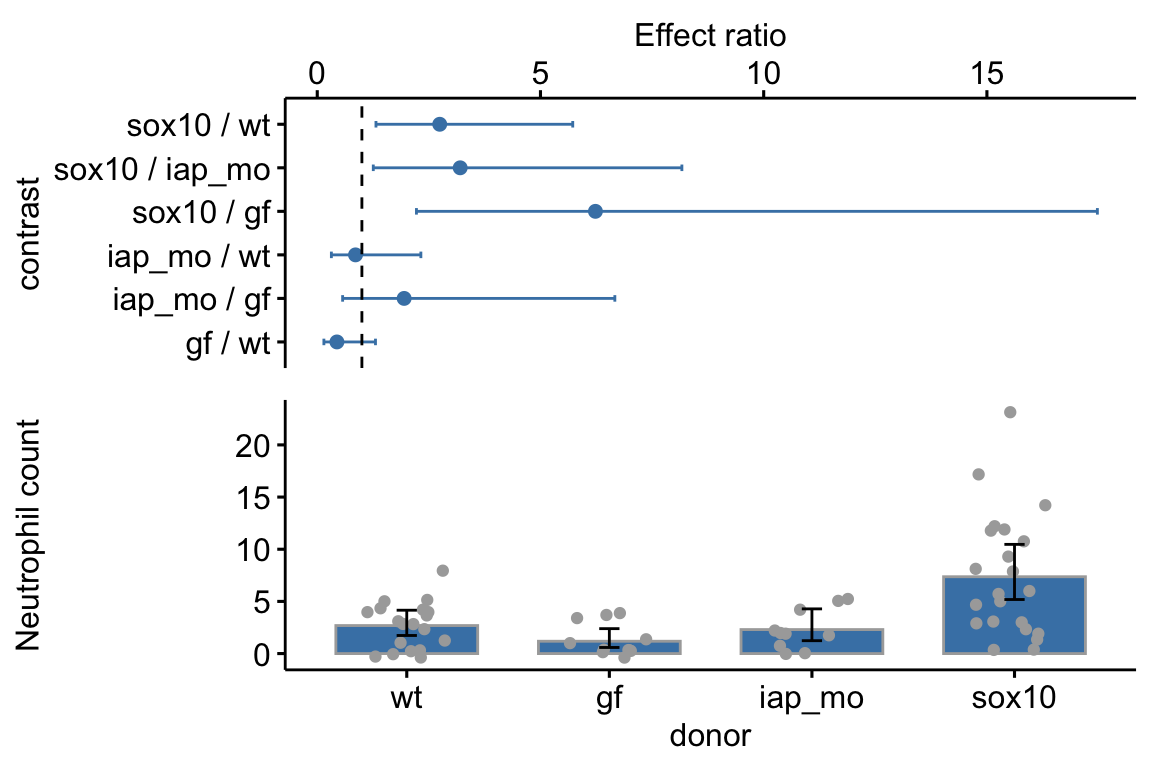
\includegraphics{Walker-elementary-statistical-modeling-draft_files/figure-latex/unnamed-chunk-62-1.pdf}

\texttt{pi3k\_long{[}treatment\ ==\ "Chow",{]})} is the subset of rows in which entries in the column ``treatment'' take the value ``Chow'' using the ``is equal'' (``=='') operator

\begin{Shaded}
\begin{Highlighting}[]
\KeywordTok{qplot}\NormalTok{(}\DataTypeTok{x =}\NormalTok{ time,}
      \DataTypeTok{y =}\NormalTok{ glucose,}
      \DataTypeTok{data =}\NormalTok{ pi3k_long[treatment }\OperatorTok{==}\StringTok{ "Chow"}\NormalTok{,],}
      \DataTypeTok{color =}\NormalTok{ treatment) }\OperatorTok{+}
\StringTok{  }\KeywordTok{geom_line}\NormalTok{(}\KeywordTok{aes}\NormalTok{(}\DataTypeTok{group =}\NormalTok{ id))}
\end{Highlighting}
\end{Shaded}

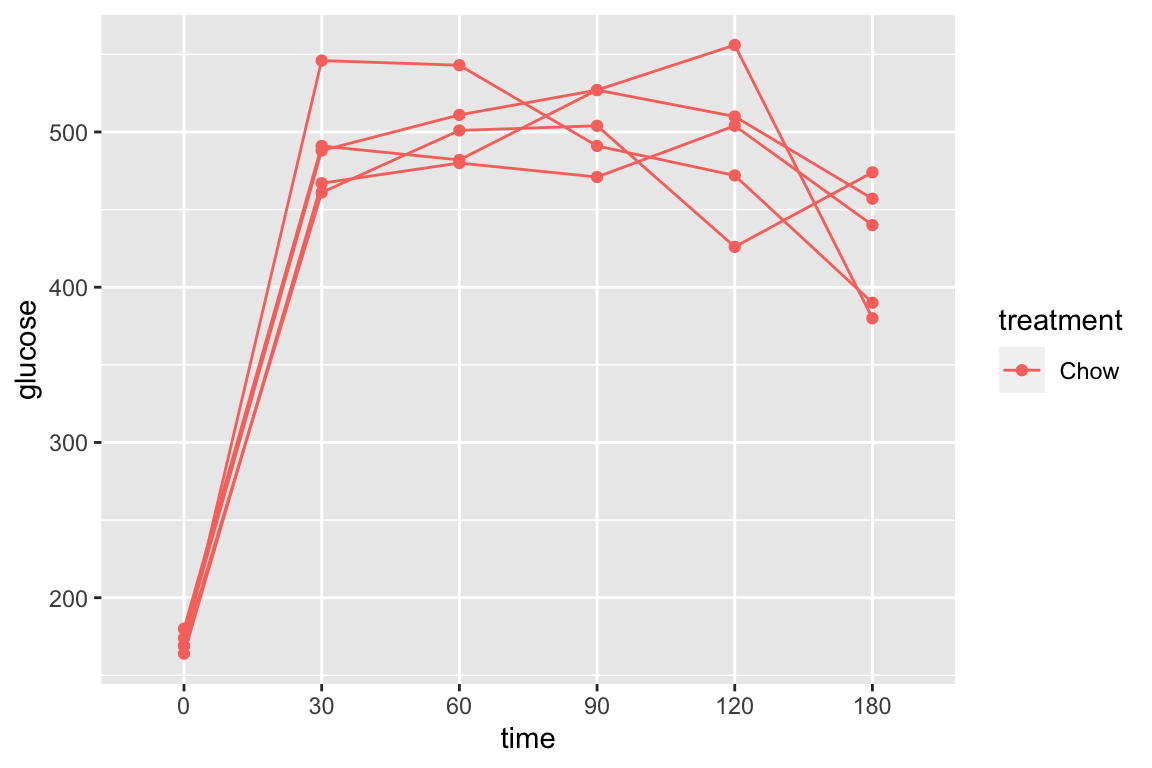
\includegraphics{Walker-elementary-statistical-modeling-draft_files/figure-latex/unnamed-chunk-63-1.pdf}

And the subset of rows in which entries in the column ``treatment'' take any value but ``Chow'' using the ``not equal'' operator (``!='').

\begin{Shaded}
\begin{Highlighting}[]
\KeywordTok{qplot}\NormalTok{(}\DataTypeTok{x =}\NormalTok{ time,}
      \DataTypeTok{y =}\NormalTok{ glucose,}
      \DataTypeTok{data =}\NormalTok{ pi3k_long[treatment }\OperatorTok{!=}\StringTok{ "Chow"}\NormalTok{,],}
      \DataTypeTok{color =}\NormalTok{ treatment) }\OperatorTok{+}
\StringTok{  }\KeywordTok{geom_line}\NormalTok{(}\KeywordTok{aes}\NormalTok{(}\DataTypeTok{group =}\NormalTok{ id))}
\end{Highlighting}
\end{Shaded}

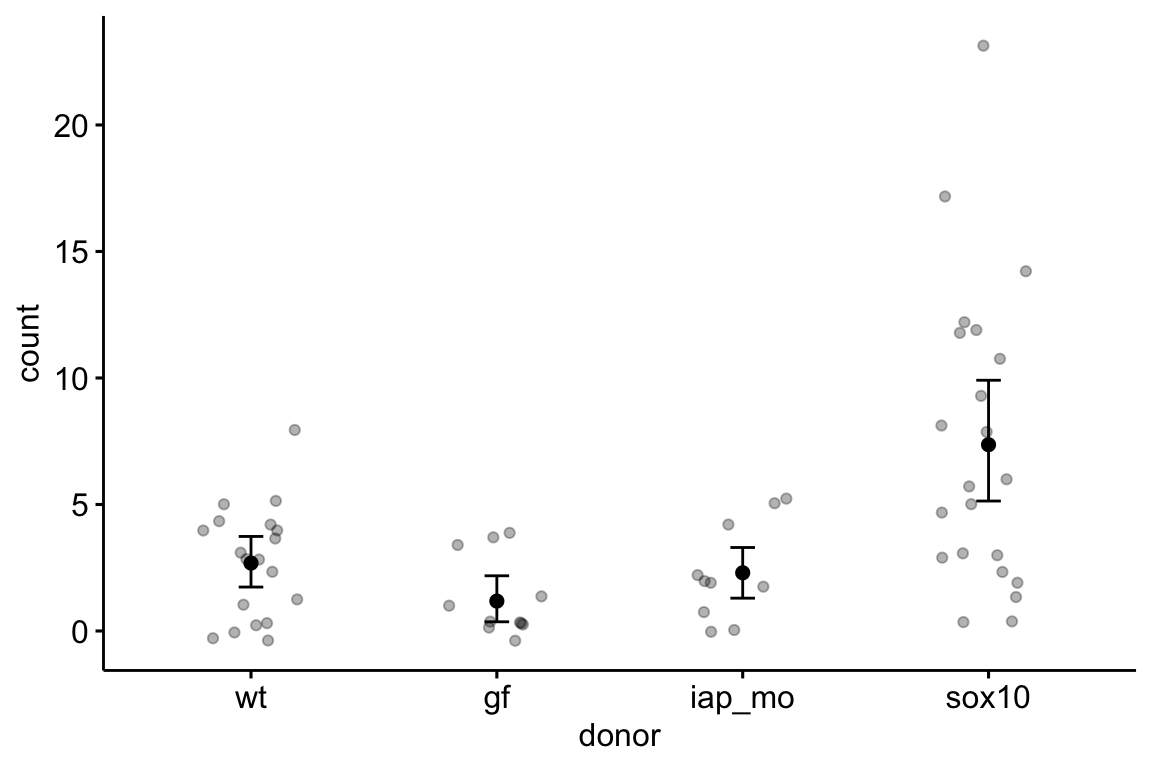
\includegraphics{Walker-elementary-statistical-modeling-draft_files/figure-latex/unnamed-chunk-64-1.pdf}

The subset of rows in which entries in the column ``treatment'' take either the value ``Chow'' or the value ``SGLT2i'' by combining two ``is equal'' (``=='') operators using the OR (``\textbar{}'') boolean operator

\begin{Shaded}
\begin{Highlighting}[]
\KeywordTok{qplot}\NormalTok{(}\DataTypeTok{x =}\NormalTok{ time,}
      \DataTypeTok{y =}\NormalTok{ glucose,}
      \DataTypeTok{data =}\NormalTok{ pi3k_long[treatment }\OperatorTok{==}\StringTok{ "Chow"} \OperatorTok{|}\StringTok{ }\NormalTok{treatment }\OperatorTok{==}\StringTok{ "SGLT2i"}\NormalTok{,],}
      \DataTypeTok{color =}\NormalTok{ treatment) }\OperatorTok{+}
\StringTok{  }\KeywordTok{geom_line}\NormalTok{(}\KeywordTok{aes}\NormalTok{(}\DataTypeTok{group =}\NormalTok{ id))}
\end{Highlighting}
\end{Shaded}

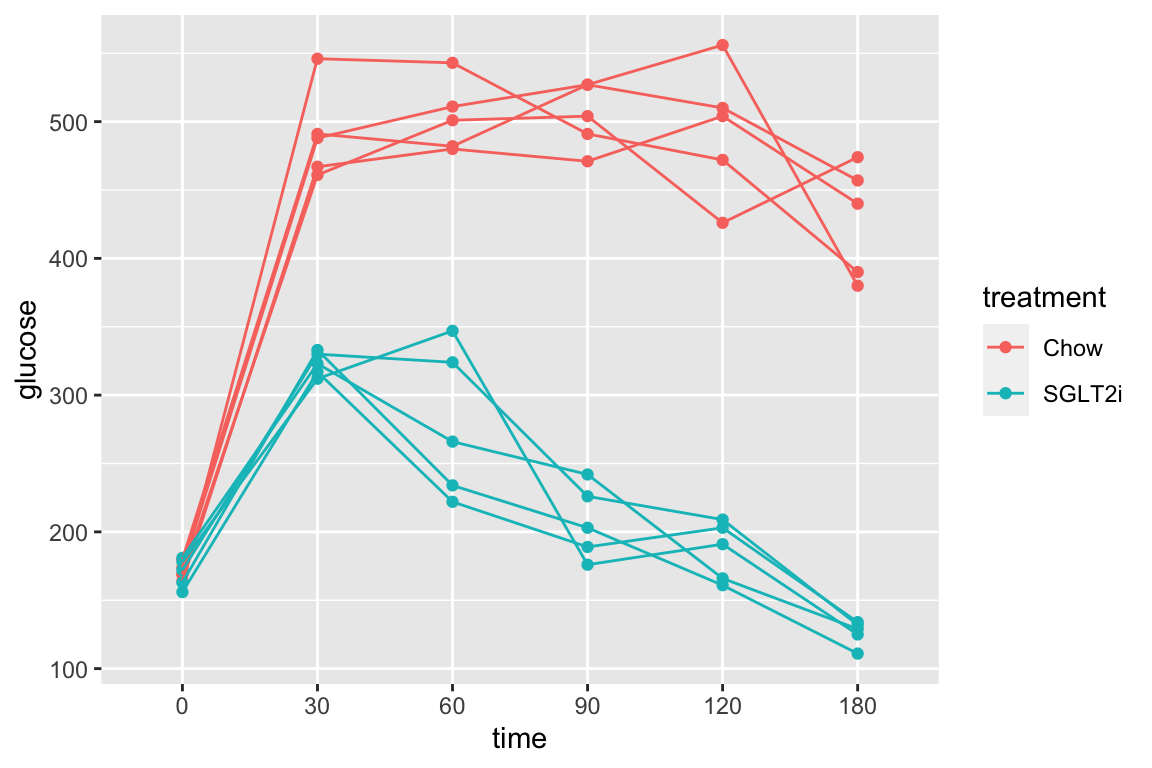
\includegraphics{Walker-elementary-statistical-modeling-draft_files/figure-latex/unnamed-chunk-65-1.pdf}

The subset of rows in which entries in the column ``time'' take either the value ``30'' or the value ``60'' using the ``in a list'' operator (\%in\%). The values in the ``time'' column look like integers but are actually treatment levels (which act like string or character variables).

\begin{Shaded}
\begin{Highlighting}[]
\KeywordTok{qplot}\NormalTok{(}\DataTypeTok{x =}\NormalTok{ time,}
      \DataTypeTok{y =}\NormalTok{ glucose,}
      \DataTypeTok{data =}\NormalTok{ pi3k_long[time  }\OperatorTok\StringTok{ }\KeywordTok{c}\NormalTok{(}\StringTok{"30"}\NormalTok{, }\StringTok{"60"}\NormalTok{),],}
      \DataTypeTok{color =}\NormalTok{ treatment) }\OperatorTok{+}
\StringTok{  }\KeywordTok{geom_line}\NormalTok{(}\KeywordTok{aes}\NormalTok{(}\DataTypeTok{group =}\NormalTok{ id))}
\end{Highlighting}
\end{Shaded}

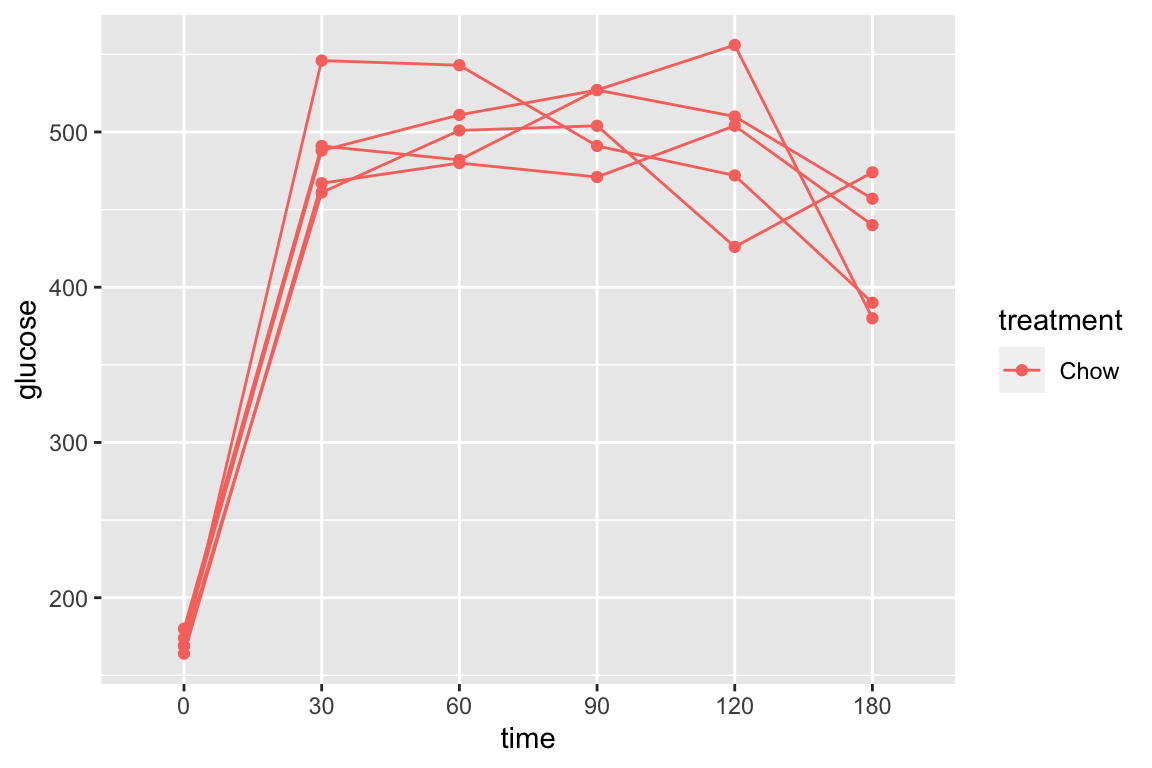
\includegraphics{Walker-elementary-statistical-modeling-draft_files/figure-latex/unnamed-chunk-66-1.pdf}

The subset of rows in which entries in the column ``time\_c'' are less than or equal to 60 using the ``less than or equal to'' operator AND the value in the treatment column is in the list (``Chow'', ``SGLT2i''). The two comparisons are combined with the AND (``\&'') Boolean operator.

\begin{Shaded}
\begin{Highlighting}[]
\NormalTok{pi3k_long[, time_c }\OperatorTok{:}\ErrorTok{=}\StringTok{ }\KeywordTok{as.numeric}\NormalTok{(}\KeywordTok{as.character}\NormalTok{(time))]}
\KeywordTok{qplot}\NormalTok{(}\DataTypeTok{x =}\NormalTok{ time,}
      \DataTypeTok{y =}\NormalTok{ glucose,}
      \DataTypeTok{data =}\NormalTok{ pi3k_long[time_c }\OperatorTok{<=}\StringTok{ }\DecValTok{30} \OperatorTok{&}\StringTok{ }\NormalTok{treatment }\OperatorTok\StringTok{ }\KeywordTok{c}\NormalTok{(}\StringTok{"Chow"}\NormalTok{, }\StringTok{"SGLT2i"}\NormalTok{),],}
      \DataTypeTok{color =}\NormalTok{ treatment) }\OperatorTok{+}
\StringTok{  }\KeywordTok{geom_line}\NormalTok{(}\KeywordTok{aes}\NormalTok{(}\DataTypeTok{group =}\NormalTok{ id))}
\end{Highlighting}
\end{Shaded}

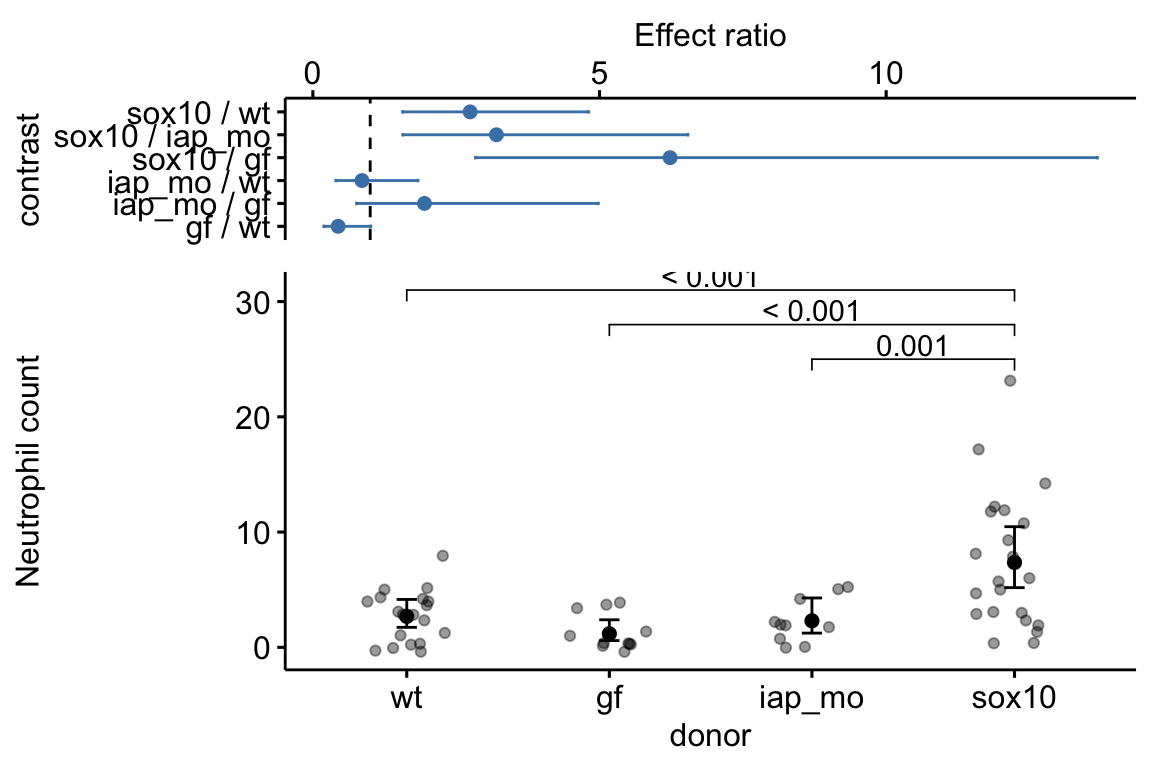
\includegraphics{Walker-elementary-statistical-modeling-draft_files/figure-latex/unnamed-chunk-67-1.pdf}

The same result as above but using different operators. I would describe this as, the subset of rows in which entries in the column ``time\_c'' are less than or equal to 60 using the ``less than or equal to'' operator AND the value in the treatment column is either ``Chow'' OR ``SGLT2i''. The two comparisons are combined with the AND (``\&'') Boolean operator. The order of operations is determined by the parentheses, as with all algebra.

\begin{Shaded}
\begin{Highlighting}[]
\NormalTok{pi3k_long[, time_c }\OperatorTok{:}\ErrorTok{=}\StringTok{ }\KeywordTok{as.numeric}\NormalTok{(}\KeywordTok{as.character}\NormalTok{(time))]}
\KeywordTok{qplot}\NormalTok{(}\DataTypeTok{x =}\NormalTok{ time,}
      \DataTypeTok{y =}\NormalTok{ glucose,}
      \DataTypeTok{data =}\NormalTok{ pi3k_long[time_c }\OperatorTok{<=}\StringTok{ }\DecValTok{30} \OperatorTok{&}\StringTok{ }\NormalTok{(treatment }\OperatorTok{==}\StringTok{ "Chow"} \OperatorTok{|}\StringTok{ }\NormalTok{treatment }\OperatorTok{==}\StringTok{ "SGLT2i"}\NormalTok{),],}
      \DataTypeTok{color =}\NormalTok{ treatment) }\OperatorTok{+}
\StringTok{  }\KeywordTok{geom_line}\NormalTok{(}\KeywordTok{aes}\NormalTok{(}\DataTypeTok{group =}\NormalTok{ id))}
\end{Highlighting}
\end{Shaded}

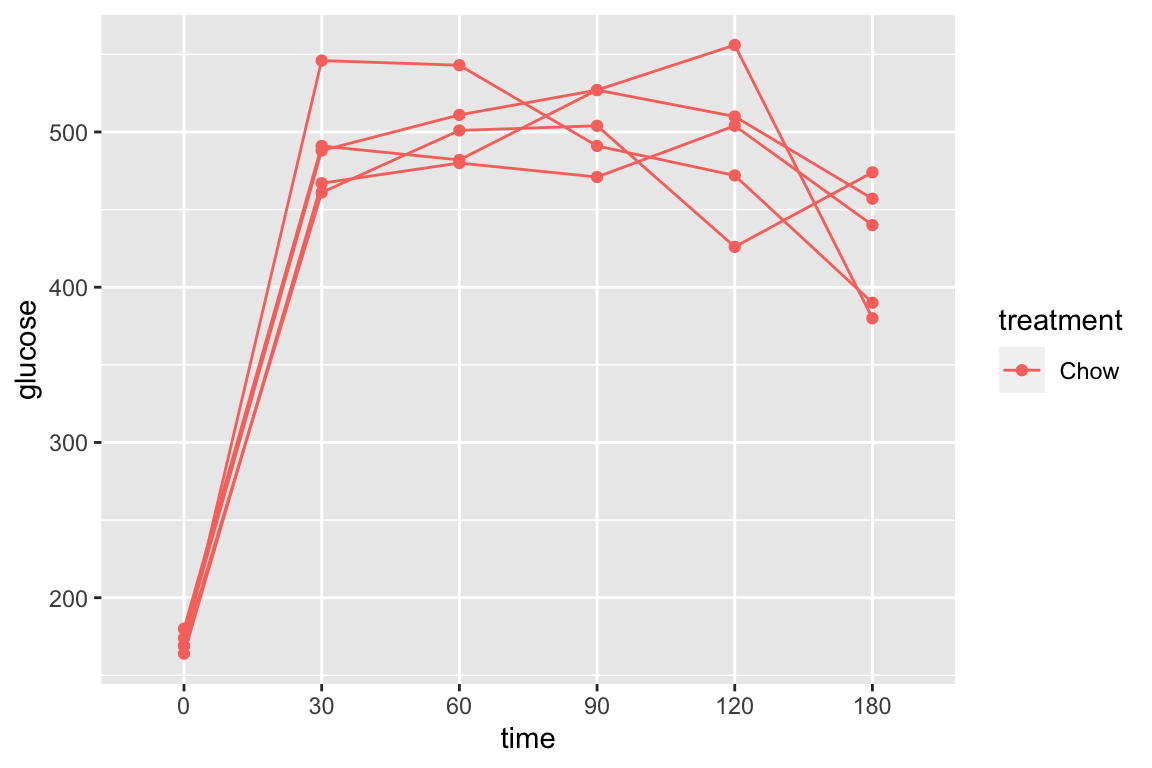
\includegraphics{Walker-elementary-statistical-modeling-draft_files/figure-latex/unnamed-chunk-68-1.pdf}

\hypertarget{wrangling-columns}{%
\subsection{Wrangling columns}\label{wrangling-columns}}

\hypertarget{creating-new-columns-that-are-functions-of-values-in-existing-columnes}{%
\subsubsection{Creating new columns that are functions of values in existing columnes}\label{creating-new-columns-that-are-functions-of-values-in-existing-columnes}}

\hypertarget{change-the-reference-level-of-a-factor}{%
\subsubsection{Change the reference level of a factor}\label{change-the-reference-level-of-a-factor}}

\hypertarget{converting-a-single-column-with-all-combinations-of-a-2-x-2-factorial-experiment-into-two-columns-each-containing-the-two-levels-of-a-factor}{%
\subsubsection{Converting a single column with all combinations of a 2 x 2 factorial experiment into two columns, each containing the two levels of a factor}\label{converting-a-single-column-with-all-combinations-of-a-2-x-2-factorial-experiment-into-two-columns-each-containing-the-two-levels-of-a-factor}}

\textbf{Article source}: Tauriello, D., Palomo-Ponce, S., Stork, D. et al.~TGFβ drives immune evasion in genetically reconstituted colon cancer metastasis. Nature 554, 538--543 (2018) \url{doi:10.1038/nature25492}

\textbf{Data source}: \url{https://www.nature.com/articles/nature25492\#Sec23}

filename: ``41586\_2018\_BFnature25492\_MOESM10\_ESM.xlsx''

sheet: ``Fig. 4h-tumours''

The analysis of the data in Fig. 4h specifies a single \(X\) variable ``Treatment'' with four levels (or groups): ``Con'', ``Gal'', ``aPD-L1'', and ``Gal+aPD-L1''. These levels indicate that the design is actually \textbf{factorial} with two factors, each with two levels. The first factor has levels ``no Gal'' and ``Gal''. The second factor has levels ``no aPD-L1'', ``aPD-L1''. The single column Treatment ``flattens'' the 2 X 2 factorial design to a 4 x 1 design. In general, we would want to analyze an experiment like this as factorial model, because this allows us to make inferences about the \emph{interaction effect} between the two factors. For these inferences, we need a standard error, or a confidence interval, or a \emph{p}-value of the estimate, which we can easily get from the factorial model. In order to analyze the data with a factorial model, we need to create two new columns -- one column is the factor variable containing the two levels of Gal and one column is the factor variable containing the two levels of aPD-L1.

\begin{Shaded}
\begin{Highlighting}[]
\NormalTok{gal_levels <-}\StringTok{ }\KeywordTok{c}\NormalTok{(}\StringTok{"no Gal"}\NormalTok{, }\StringTok{"Gal"}\NormalTok{)}
\NormalTok{tumor[, gal }\OperatorTok{:}\ErrorTok{=}\StringTok{ }\KeywordTok{ifelse}\NormalTok{(treatment }\OperatorTok{==}\StringTok{ "Gal"} \OperatorTok{|}\StringTok{ }\NormalTok{treatment }\OperatorTok{==}\StringTok{ "Gal+aPD-L1"}\NormalTok{,}
\NormalTok{                      gal_levels[}\DecValTok{2}\NormalTok{],}
\NormalTok{                      gal_levels[}\DecValTok{1}\NormalTok{])]}

\NormalTok{apd_levels <-}\StringTok{ }\KeywordTok{c}\NormalTok{(}\StringTok{"no aPD-L1"}\NormalTok{, }\StringTok{"aPD-L1"}\NormalTok{)}
\NormalTok{tumor[, apdl1 }\OperatorTok{:}\ErrorTok{=}\StringTok{ }\KeywordTok{ifelse}\NormalTok{(treatment }\OperatorTok{==}\StringTok{ "aPD-L1"} \OperatorTok{|}\StringTok{ }\NormalTok{treatment }\OperatorTok{==}\StringTok{ "Gal+aPD-L1"}\NormalTok{,}
\NormalTok{                      apd_levels[}\DecValTok{2}\NormalTok{],}
\NormalTok{                      apd_levels[}\DecValTok{1}\NormalTok{])]}

\CommentTok{# re-order factor levels}
\NormalTok{tumor[, gal}\OperatorTok{:}\ErrorTok{=}\KeywordTok{factor}\NormalTok{(gal, gal_levels)]}
\NormalTok{tumor[, apdl1}\OperatorTok{:}\ErrorTok{=}\KeywordTok{factor}\NormalTok{(apdl1, apd_levels)]}
\end{Highlighting}
\end{Shaded}

A way to check the results to make sure that our conversion is correct is to compute the sampel size for the 2 x 2 combinations, but include the original treatment column in the \texttt{by} list.

\begin{Shaded}
\begin{Highlighting}[]
\NormalTok{tumor[}\OperatorTok{!}\KeywordTok{is.na}\NormalTok{(num_positive_per_mm), .(}\DataTypeTok{N=}\NormalTok{.N), by=.(treatment, gal, apdl1)]}
\end{Highlighting}
\end{Shaded}

\begin{verbatim}
##     treatment    gal     apdl1   N
## 1:        Con no Gal no aPD-L1 124
## 2:        Gal    Gal no aPD-L1  89
## 3:     aPD-L1 no Gal    aPD-L1 101
## 4: Gal+aPD-L1    Gal    aPD-L1  58
\end{verbatim}

That looks good.

\textbf{Bug alert} If you break Rule \#1, and type in the treatment level ``Gal+aPD-L1'' as ``Gal + aPD-L1'', then you will get new columns containing junk.

\begin{verbatim}
##     treatment    gal     apdl1   N
## 1:        Con no Gal no aPD-L1 124
## 2:        Gal    Gal no aPD-L1  89
## 3:     aPD-L1 no Gal    aPD-L1 101
## 4: Gal+aPD-L1 no Gal no aPD-L1  58
\end{verbatim}

Remember Rule \#1. Always copy and paste any text that will be inserted into quotes. This is easily done here by typing \texttt{unique(tumor\$treatment)} into the console. This function returns the unique values of the column ``treatment'' of the data.table ``tumor''.

\begin{quote}
unique(tumor\$treatment)
{[}1{]} ``Con'' ``Gal'' ``aPD-L1'' ``Gal+aPD-L1''
\end{quote}

Now, copy the name of a level and paste into your code. Repeat until done.

\hypertarget{missing-data}{%
\subsection{Missing data}\label{missing-data}}

Source: \href{https://journals.plos.org/plosgenetics/article?id=10.1371/journal.pgen.1008002\&rev=1}{Deletion of Cdkn1b in ACI rats leads to increased proliferation and pregnancy-associated changes in the mammary gland due to perturbed systemic endocrine environment}

Supplement Figure 1F of this paper shows weight as a function of age class and genotype for the whole body and 8 organs. There are some missing weights in the Excel-archived data. These missing data are designated with a minus ``-'' sign. To import these data in correctly, use the \texttt{na\ =} argument in the \texttt{read\_excel} function.

\begin{Shaded}
\begin{Highlighting}[]
\NormalTok{file_folder <-}\StringTok{ "Deletion of Cdkn1b in ACI rats leads to increased proliferation and pregnancy-associated changes in the mammary gland due to perturbed systemic endocrine environment"}
\NormalTok{file_name <-}\StringTok{ "journal.pgen.1008002.s008.xlsx"}
\NormalTok{file_path <-}\StringTok{ }\KeywordTok{here}\NormalTok{(data_folder, file_folder, file_name)}
  
\NormalTok{fig_s1f <-}\StringTok{ }\KeywordTok{read_excel}\NormalTok{(file_path,}
                    \DataTypeTok{sheet =} \StringTok{"all weights"}\NormalTok{,}
                    \DataTypeTok{range =} \StringTok{"A2:K57"}\NormalTok{,}
                    \DataTypeTok{na =} \StringTok{"-"}\NormalTok{,}
                    \DataTypeTok{col_names =} \OtherTok{TRUE}\NormalTok{) }\OperatorTok
\StringTok{  }\KeywordTok{clean_names}\NormalTok{() }\OperatorTok
\StringTok{  }\KeywordTok{data.table}\NormalTok{()}

\NormalTok{fig_s1f[, genotype }\OperatorTok{:}\ErrorTok{=}\StringTok{ }\KeywordTok{factor}\NormalTok{(genotype, }\KeywordTok{c}\NormalTok{(}\StringTok{"+/+"}\NormalTok{, }\StringTok{"-/-"}\NormalTok{))]}
\NormalTok{fig_s1f[, age_class }\OperatorTok{:}\ErrorTok{=}\StringTok{ }\KeywordTok{ifelse}\NormalTok{(age_at_sac_wks }\OperatorTok{<=}\StringTok{ }\FloatTok{6.0}\NormalTok{, }\StringTok{"4-6"}\NormalTok{, }\StringTok{"8+"}\NormalTok{)]}

\CommentTok{# View(fig_s1f)}
\end{Highlighting}
\end{Shaded}

Notes

\begin{enumerate}
\def\labelenumi{\arabic{enumi}.}
\tightlist
\item
  In R, a value of ``NA'' represents missing.
\item
  The default value for \texttt{na\ =} is an empty (or blank) cell (not a space but a cell that is empty).
\item
  \texttt{na\ =} accepts a list of strings, for example \texttt{na\ =\ c("",\ "-99",\ "-\/-")} that will all be read as na.
\end{enumerate}

\hypertarget{handling-missing-data}{%
\subsubsection{Handling missing data}\label{handling-missing-data}}

\hypertarget{many-base-r-functions-used-for-summary-measures-require-na-handling}{%
\paragraph{Many base R functions used for summary measures require NA handling}\label{many-base-r-functions-used-for-summary-measures-require-na-handling}}

\begin{Shaded}
\begin{Highlighting}[]
\KeywordTok{mean}\NormalTok{(fig_s1f[, ovary]) }\CommentTok{# returns "NA"}
\end{Highlighting}
\end{Shaded}

\begin{verbatim}
## [1] NA
\end{verbatim}

\begin{Shaded}
\begin{Highlighting}[]
\KeywordTok{mean}\NormalTok{(fig_s1f[, ovary], }\DataTypeTok{na.rm =} \OtherTok{TRUE}\NormalTok{) }\CommentTok{# returns the mean}
\end{Highlighting}
\end{Shaded}

\begin{verbatim}
## [1] 0.2489524
\end{verbatim}

\begin{Shaded}
\begin{Highlighting}[]
\KeywordTok{sd}\NormalTok{(fig_s1f[, ovary]) }\CommentTok{# returns "NA"}
\end{Highlighting}
\end{Shaded}

\begin{verbatim}
## [1] NA
\end{verbatim}

\begin{Shaded}
\begin{Highlighting}[]
\KeywordTok{sd}\NormalTok{(fig_s1f[, ovary], }\DataTypeTok{na.rm =} \OtherTok{TRUE}\NormalTok{) }\CommentTok{# returns the mean}
\end{Highlighting}
\end{Shaded}

\begin{verbatim}
## [1] 0.151694
\end{verbatim}

\begin{Shaded}
\begin{Highlighting}[]
\KeywordTok{sum}\NormalTok{(fig_s1f[, ovary]) }\CommentTok{# returns "NA"}
\end{Highlighting}
\end{Shaded}

\begin{verbatim}
## [1] NA
\end{verbatim}

\begin{Shaded}
\begin{Highlighting}[]
\KeywordTok{sum}\NormalTok{(fig_s1f[, ovary], }\DataTypeTok{na.rm =} \OtherTok{TRUE}\NormalTok{) }\CommentTok{# returns the mean}
\end{Highlighting}
\end{Shaded}

\begin{verbatim}
## [1] 10.456
\end{verbatim}

There are many ways to get the sample size for a particular variable. Be careful if using \texttt{length()} which counts NA as part of the vector of values.

\hypertarget{the-is.na-function-is-useful}{%
\paragraph{The !is.na function is useful}\label{the-is.na-function-is-useful}}

\begin{Shaded}
\begin{Highlighting}[]
\KeywordTok{length}\NormalTok{(fig_s1f[, ovary])}
\end{Highlighting}
\end{Shaded}

\begin{verbatim}
## [1] 55
\end{verbatim}

\begin{Shaded}
\begin{Highlighting}[]
\KeywordTok{length}\NormalTok{(fig_s1f[}\OperatorTok{!}\KeywordTok{is.na}\NormalTok{(ovary), ovary])}
\end{Highlighting}
\end{Shaded}

\begin{verbatim}
## [1] 42
\end{verbatim}

Notes

\begin{enumerate}
\def\labelenumi{\arabic{enumi}.}
\tightlist
\item
  \texttt{!is.na(ovary)} is taking the subset of rows of fig\_s1f for which the value of ``ovary'' is not NA (!is.na is read ``not is.na'')
\end{enumerate}

This is especially useful if you are creating your own code uses counts. Here I create a table of means, standard error of the mean, and 95\% CIs of the mean for each genotype group. But first, this script generates the wrong N for each group (since there are missing values), although the mean and SD are correct.

\begin{Shaded}
\begin{Highlighting}[]
\NormalTok{fig_s1f[, .(}\DataTypeTok{mean =} \KeywordTok{mean}\NormalTok{(spleen, }\DataTypeTok{na.rm =} \OtherTok{TRUE}\NormalTok{),}
            \DataTypeTok{n =}\NormalTok{ .N,}
            \DataTypeTok{sd =} \KeywordTok{sd}\NormalTok{(spleen, }\DataTypeTok{na.rm =} \OtherTok{TRUE}\NormalTok{)),}
\NormalTok{        by =}\StringTok{ }\NormalTok{genotype]}
\end{Highlighting}
\end{Shaded}

\begin{verbatim}
##    genotype      mean  n         sd
## 1:      -/- 0.5801333 21 0.13680480
## 2:      +/+ 0.2956667 34 0.04460855
\end{verbatim}

To compute the correct \emph{n}, which will be necessary for computing the SE and the CI, use \texttt{!is.na}

\begin{Shaded}
\begin{Highlighting}[]
\NormalTok{spleen_summary <-}\StringTok{ }\NormalTok{fig_s1f[}\OperatorTok{!}\KeywordTok{is.na}\NormalTok{(spleen), .(}\DataTypeTok{mean =} \KeywordTok{mean}\NormalTok{(spleen),}
            \DataTypeTok{n =}\NormalTok{ .N,}
            \DataTypeTok{sd =} \KeywordTok{sd}\NormalTok{(spleen)),}
\NormalTok{        by =}\StringTok{ }\NormalTok{genotype]}
\NormalTok{spleen_summary[, se }\OperatorTok{:}\ErrorTok{=}\StringTok{ }\NormalTok{sd}\OperatorTok{/}\KeywordTok{sqrt}\NormalTok{(n)]}
\NormalTok{spleen_summary[, lower }\OperatorTok{:}\ErrorTok{=}\StringTok{ }\NormalTok{mean }\OperatorTok{+}\StringTok{ }\NormalTok{se}\OperatorTok{*}\KeywordTok{qt}\NormalTok{(.}\DecValTok{025}\NormalTok{, (n}\DecValTok{-1}\NormalTok{))]}
\NormalTok{spleen_summary[, upper }\OperatorTok{:}\ErrorTok{=}\StringTok{ }\NormalTok{mean }\OperatorTok{+}\StringTok{ }\NormalTok{se}\OperatorTok{*}\KeywordTok{qt}\NormalTok{(.}\DecValTok{975}\NormalTok{, (n}\DecValTok{-1}\NormalTok{))]}
\NormalTok{spleen_summary}
\end{Highlighting}
\end{Shaded}

\begin{verbatim}
##    genotype      mean  n         sd         se     lower     upper
## 1:      -/- 0.5801333 15 0.13680480 0.03532285 0.5043734 0.6558933
## 2:      +/+ 0.2956667 27 0.04460855 0.00858492 0.2780201 0.3133132
\end{verbatim}

\hypertarget{ggplot-functions-automatically-handle-missing-values}{%
\paragraph{ggplot functions automatically handle missing values}\label{ggplot-functions-automatically-handle-missing-values}}

with a useful warning.

\begin{Shaded}
\begin{Highlighting}[]
\KeywordTok{qplot}\NormalTok{(}\DataTypeTok{x =}\NormalTok{ body_wt_g_sac,}
      \DataTypeTok{y =}\NormalTok{ spleen,}
      \DataTypeTok{color =}\NormalTok{ genotype,}
      \DataTypeTok{data =}\NormalTok{ fig_s1f)}
\end{Highlighting}
\end{Shaded}

\begin{verbatim}
## Warning: Removed 13 rows containing missing values (geom_point).
\end{verbatim}

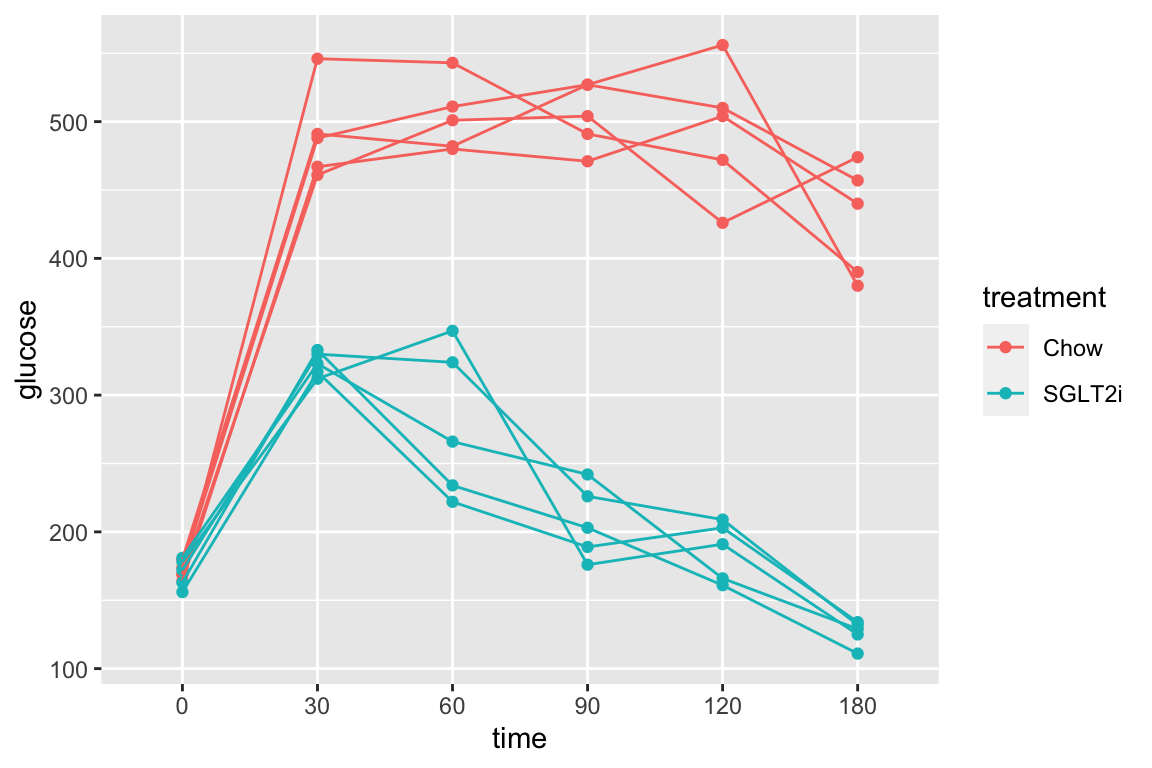
\includegraphics{Walker-elementary-statistical-modeling-draft_files/figure-latex/unnamed-chunk-78-1.pdf}

\hypertarget{regression-model-functions-lm-glm-gls-etc.-handle-missing-values-by-default}{%
\paragraph{Regression model functions (lm, glm, gls, etc.) handle missing values by default}\label{regression-model-functions-lm-glm-gls-etc.-handle-missing-values-by-default}}

Missing data in regression model functions such as \texttt{lm} are handled using the argument \texttt{na.action\ =} and the default is ``na.omit'', which omits any rows that contain a missing value in one or more of the model variables (it includes rows if these contain missing values only in the columns not included in the model). It's as if the user took the subset of data including only the columns containing the model variables and then deleted any row with missing values.

Here is the coefficient table of the fit model object that did not explictly tell the \texttt{lm} function how to handle missing data.

\begin{Shaded}
\begin{Highlighting}[]
\NormalTok{m1 <-}\StringTok{ }\KeywordTok{lm}\NormalTok{(spleen }\OperatorTok{~}\StringTok{ }\NormalTok{body_wt_g_sac }\OperatorTok{+}\StringTok{ }\NormalTok{genotype,}
         \DataTypeTok{data =}\NormalTok{ fig_s1f)}
\KeywordTok{coef}\NormalTok{(}\KeywordTok{summary}\NormalTok{(m1))}
\end{Highlighting}
\end{Shaded}

\begin{verbatim}
##                 Estimate   Std. Error   t value     Pr(>|t|)
## (Intercept)   0.04238009 0.0242993900  1.744081 8.902319e-02
## body_wt_g_sac 0.00167493 0.0001506493 11.118067 1.170042e-13
## genotype-/-   0.23760586 0.0147600545 16.097898 8.072069e-19
\end{verbatim}

Here is the coefficient table of the fit model object that did explicitly tell \texttt{lm} how to handle missing data, using the argument \texttt{na.action\ =\ "na.exclude"}. These coefficient tables are the same.

\begin{Shaded}
\begin{Highlighting}[]
\NormalTok{m2 <-}\StringTok{ }\KeywordTok{lm}\NormalTok{(spleen }\OperatorTok{~}\StringTok{ }\NormalTok{body_wt_g_sac }\OperatorTok{+}\StringTok{ }\NormalTok{genotype,}
         \DataTypeTok{data =}\NormalTok{ fig_s1f,}
         \DataTypeTok{na.action =} \StringTok{"na.exclude"}\NormalTok{)}
\KeywordTok{coef}\NormalTok{(}\KeywordTok{summary}\NormalTok{(m2))}
\end{Highlighting}
\end{Shaded}

\begin{verbatim}
##                 Estimate   Std. Error   t value     Pr(>|t|)
## (Intercept)   0.04238009 0.0242993900  1.744081 8.902319e-02
## body_wt_g_sac 0.00167493 0.0001506493 11.118067 1.170042e-13
## genotype-/-   0.23760586 0.0147600545 16.097898 8.072069e-19
\end{verbatim}

\hypertarget{butbeware-of-fitted-predicted-or-residual-values-from-regression-model-functions-unless-youve-explictly-told-the-function-how-to-handle-missing-values}{%
\subsubsection{But\ldots beware of fitted, predicted, or residual values from regression model functions unless you've explictly told the function how to handle missing values}\label{butbeware-of-fitted-predicted-or-residual-values-from-regression-model-functions-unless-youve-explictly-told-the-function-how-to-handle-missing-values}}

\textbf{Use \texttt{na.action\ =\ "na.exclude"}} if you want to add the fitted (or predicted) values or residuals as new columns in the original data object (fig\_sf1). Compare the length of the fitted values vector from models m1 (using the default ``na.omit'') and m2 (using the ``na.exclude'').

\begin{Shaded}
\begin{Highlighting}[]
\KeywordTok{length}\NormalTok{(}\KeywordTok{fitted}\NormalTok{(m1))}
\end{Highlighting}
\end{Shaded}

\begin{verbatim}
## [1] 42
\end{verbatim}

\begin{Shaded}
\begin{Highlighting}[]
\KeywordTok{length}\NormalTok{(}\KeywordTok{fitted}\NormalTok{(m2))}
\end{Highlighting}
\end{Shaded}

\begin{verbatim}
## [1] 55
\end{verbatim}

There are 55 observations (rows in the data) but only 42 complete rows with no missing values. The vector of fitted values from m1 has 42 fitted values. The vector of fitted values from m2 has 55 elements, the 42 fitted values plus 13 NA elements.

This is important if we want to do something like add the fitted values (or residuals, or some function of these) to the original data object (fig\_sf1). Here I compute the spleen weights adjusted to the mean body weight of the control (``+/+'') group using the residuals from m1 and m2.

\begin{Shaded}
\begin{Highlighting}[]
\NormalTok{mean_x_control <-}\StringTok{ }\KeywordTok{mean}\NormalTok{(fig_s1f[genotype }\OperatorTok{==}\StringTok{ "+/+"}\NormalTok{, body_wt_g_sac])}
\NormalTok{b <-}\StringTok{ }\KeywordTok{coef}\NormalTok{(m1)}
\NormalTok{fig_s1f[, spleen_adj_m1 }\OperatorTok{:}\ErrorTok{=}\StringTok{ }\NormalTok{b[}\DecValTok{1}\NormalTok{] }\OperatorTok{+}
\StringTok{          }\NormalTok{b[}\DecValTok{2}\NormalTok{]}\OperatorTok{*}\NormalTok{mean_x_control }\OperatorTok{+}
\StringTok{          }\NormalTok{b[}\DecValTok{3}\NormalTok{]}\OperatorTok{*}\NormalTok{(}\KeywordTok{as.integer}\NormalTok{(genotype)}\OperatorTok{-}\DecValTok{1} \OperatorTok{+}
\StringTok{          }\KeywordTok{residuals}\NormalTok{(m1))]}
\end{Highlighting}
\end{Shaded}

\begin{verbatim}
## Warning in as.integer(genotype) - 1 + residuals(m1): longer object length
## is not a multiple of shorter object length
\end{verbatim}

\begin{Shaded}
\begin{Highlighting}[]
\NormalTok{fig_s1f[, spleen_adj_m2 }\OperatorTok{:}\ErrorTok{=}\StringTok{ }\NormalTok{b[}\DecValTok{1}\NormalTok{] }\OperatorTok{+}
\StringTok{          }\NormalTok{b[}\DecValTok{2}\NormalTok{]}\OperatorTok{*}\NormalTok{mean_x_control }\OperatorTok{+}
\StringTok{          }\NormalTok{b[}\DecValTok{3}\NormalTok{]}\OperatorTok{*}\NormalTok{(}\KeywordTok{as.integer}\NormalTok{(genotype)}\OperatorTok{-}\DecValTok{1} \OperatorTok{+}
\StringTok{          }\KeywordTok{residuals}\NormalTok{(m2))]}
\CommentTok{# View(fig_s1f)}
\end{Highlighting}
\end{Shaded}

The computation of ``spleen\_adj\_m1'' returns a warning that the values of \texttt{residuals(m1)} were recycled (the first 42 elements of the new column were filled with the 42 residuals and the last 13 elements of the new column were filled with the first 13 residuals) -- after the first row of missing data, all of these computed adjusted values are wrong. Using \texttt{residuals(m2}), the adjusted values are matched to the correct row and the rows with missing variables do not have an adjusted value (because there is no residual to compute this).

\hypertarget{saving-data}{%
\section{Saving data}\label{saving-data}}

For many projects, it is uncommon to save data. I might save simulated data if it takes a long time (tens of minutes to hours or even days) to generate these and I simply want to work with the simulated data in the future and not have to regenerate it. Or I might save processed data if it takes a long time to import and process and I want to analyze the processed data in the future and not have to re-import and process it.

If the data will only be used in this or future R projects, the data can be saved as an R object using \texttt{saveRDS()}

\begin{Shaded}
\begin{Highlighting}[]
\NormalTok{outfile_name <-}\StringTok{ "Prenatal acoustic communication programs offspring for high post-hatching temperatures in a songbird.Rds"}
\NormalTok{save_file_path <-}\StringTok{ }\KeywordTok{here}\NormalTok{(output_folder, outfile_name)}
\KeywordTok{saveRDS}\NormalTok{(}\DataTypeTok{object =}\NormalTok{ chick, }\DataTypeTok{file =}\NormalTok{ save_file_path)}

\CommentTok{# to read this use}
\NormalTok{chick <-}\StringTok{ }\KeywordTok{readRDS}\NormalTok{(save_file_path)}
\end{Highlighting}
\end{Shaded}

Reading a large .Rds file is very fast compared to reading the same data stored as a text file. However, if the data need to be imported into some other software, such as a spreadsheet, then save the data as a text file.

\begin{Shaded}
\begin{Highlighting}[]
\CommentTok{# save the data to output folder}

\CommentTok{# tab delimited}
\NormalTok{outfile_name <-}\StringTok{ "Prenatal acoustic communication programs offspring for high post-hatching temperatures in a songbird.txt"}
\NormalTok{save_file_path <-}\StringTok{ }\KeywordTok{here}\NormalTok{(output_folder, outfile_name)}
\KeywordTok{write.table}\NormalTok{(chick, save_file_path, }\DataTypeTok{sep=}\StringTok{"}\CharTok{\textbackslash{}t}\StringTok{"}\NormalTok{, }\DataTypeTok{quote=}\OtherTok{FALSE}\NormalTok{)}

\CommentTok{# comma delimited}
\NormalTok{outfile_name <-}\StringTok{ "Prenatal acoustic communication programs offspring for high post-hatching temperatures in a songbird.csv"}
\NormalTok{save_file_path <-}\StringTok{ }\KeywordTok{here}\NormalTok{(output_folder, outfile_name)}
\KeywordTok{write.table}\NormalTok{(chick, save_file_path, }\DataTypeTok{sep=}\StringTok{","}\NormalTok{, }\DataTypeTok{quote=}\OtherTok{FALSE}\NormalTok{)}
\end{Highlighting}
\end{Shaded}

Look at your project directory to make sure the file is where it should be! We used \texttt{write.table()} to create a tab-delimited text file using \texttt{sep="\textbackslash{}t"} to specify tabs to separate the row elements. "\t" is the standard character string for a tab. Check in your output folder and open the file in a text editor.

\hypertarget{plotting-models}{%
\chapter{Plotting Models}\label{plotting-models}}

\emph{So, along the lines of Sarah Susanka's ``Not So Big House,'' Kolbert asks the group, ``What would a Pretty Good House look like?''} -- Michael Maines\footnote{``The Pretty Good House - Finding the right balance between construction cost and energy performance''. \url{https://www.greenbuildingadvisor.com/article/the-pretty-good-house}}

When it comes to plotting, many researchers mindlessly generate plots that are easily generated by the software and look like the typical plots published in the field. The resulting plot is comforting because it is familiar, not because it effectively communicates what a good plot should communicate -- the model results.

Plots should be the focus of both the reader and researcher. Instead of mindless plotting, a researcher should ask a series of questions of every plot

\begin{enumerate}
\def\labelenumi{\arabic{enumi}.}
\tightlist
\item
  What is the point of each element in a plot?
\item
  Are these the points that I most want to communicate?
\item
  Are there better practices for communicating these points?
\item
  Are the points that I want to communicate that are not covered by these elements?
\end{enumerate}

The answer to these questions should inform what is and what is not plotted. The result is a pretty good plot. The idea of a pretty good plot is borrowed from the ``pretty good house'' concept that grew out of a collaborative group of builders and architects in Northern New England. The ``pretty good house'' combines best practices for building an earth friendly, high performance home at a reasonable cost. There is no pretty good house governing body that awards certificates of achievement but, instead, a set of metrics and a collection of building practices that can achieve these.

A typical pretty good plot contains some combination of

\begin{enumerate}
\def\labelenumi{\arabic{enumi}.}
\tightlist
\item
  Modeled effects with confidence intervals. ``Effects'' are the coefficients of a model, or contrasts constructed from the model, such as pairwise differences between the means of the levels of a factor. Inferences are typically made from the estimated effects
\item
  Modeled means and standard errors or confidence intervals.
\item
  Raw data points or a summary distribution of these.
\end{enumerate}

\hypertarget{pretty-good-plots-show-the-model-and-the-data}{%
\section{Pretty good plots show the model and the data}\label{pretty-good-plots-show-the-model-and-the-data}}

The data to introduce best practices in plotting come from ``The enteric nervous system promotes intestinal health by constraining microbiota composition''\footnote{Rolig, A.S., Mittge, E.K., Ganz, J., Troll, J.V., Melancon, E., Wiles, T.J., Alligood, K., Stephens, W.Z., Eisen, J.S. and Guillemin, K., 2017. The enteric nervous system promotes intestinal health by constraining microbiota composition. PLoS biology, 15(2), p.e2000689}. The researchers found that zebrafish with a \emph{sox10} mutation lacked an enteric nervous system and developed a microbiota-dependent inflammation. The paper includes several experiments to probe the hypothesis that the ENS regulates microbial community composition and, in turn, inflammatory status. The data here are from Fig. 2 of the paper, which reports the results of one of a set of experiments to test the hypothesis that microbiota from \emph{sox10} mutants (that induce inflammation) are necessary and sufficient to induce inflammation in wildtype guts. In this experiment, homogenized intestines and their microbial community from four different donor groups were added to the flasks housing the zebrafish. The response variable is neutrophil count. Neutrophils are a white blood cell that increase in number during inflammation. The four treatment levels are the different donors of intestinal microbes: wt (wild type), gf (germ free, so no microbes are transferred), iap\_mo (a control ``for the possibility that nonbacterial factors such as host pro-inflammatory cytokines rather than microbial derived factors cause transmissible intestinal inflammation''), and sox10.

\hypertarget{pretty-good-plot-component-1-modeled-effects-plot}{%
\subsection{Pretty good plot component 1: Modeled effects plot}\label{pretty-good-plot-component-1-modeled-effects-plot}}

Biologists infer the biological consequences of a treatment by interpreting the magnitude and sign of treatment ``effects'', such as the differences in means among treatment levels. Why then do we mostly plot treatment level means, where effects can only be inferred \emph{indirectly}, by mentally computing differences in means? Instead, our primary plots should be effects plots, which \emph{directly} communicate treatment effects, and the uncertainty in the estimates of these effects.

\begin{figure}
\centering
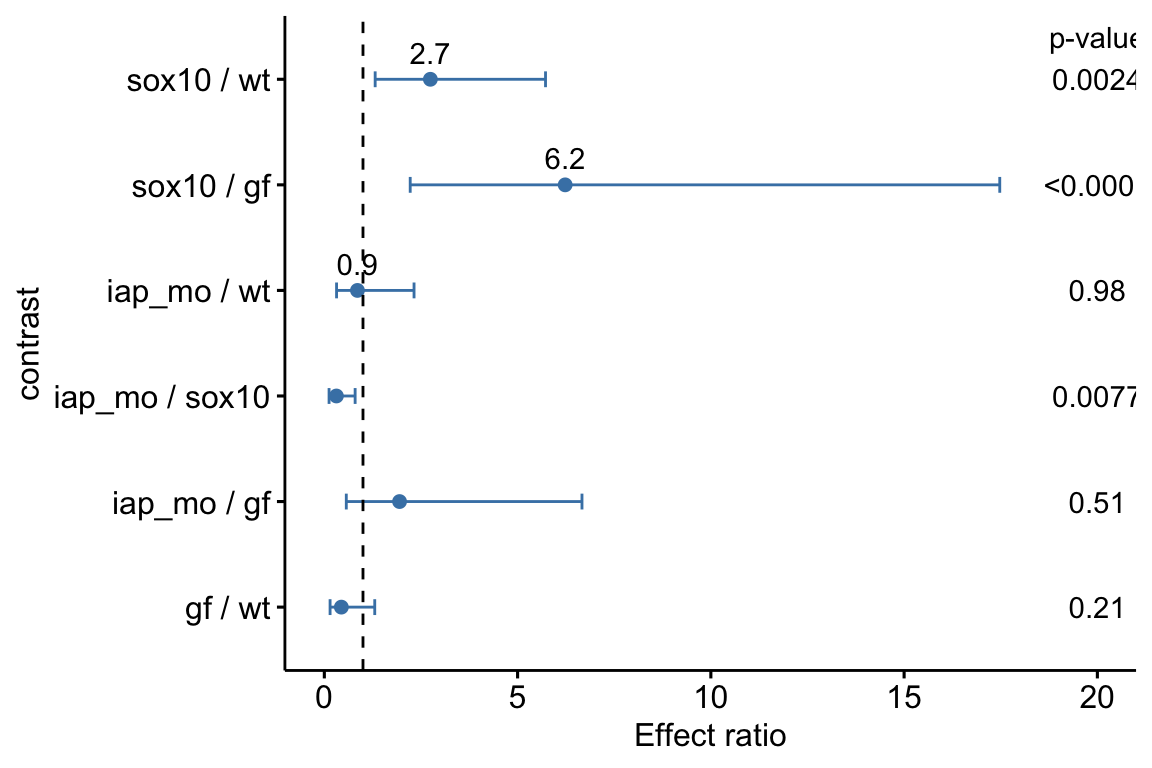
\includegraphics{Walker-elementary-statistical-modeling-draft_files/figure-latex/plots-effect-1.pdf}
\caption{\label{fig:plots-effect}Effects Plot}
\end{figure}

The y-axis contains all pairwise comparisons among the four treatment levels. The x-axis is the response, which is the ratio of the means of the two groups in the comparison. For example, the top comparison shows that guts in fish exposed to sox10 donors have 2.7X more neutrophils per length of gut than guts in fish exposed to wild type donors. The bars are 95\% confidence intervals, with is the range of effects that are compatible with the observed data at the 95\% level (confidence intervals are disscussed in depth in chapter xxx.). The small end of the interval for the sox10/wt comparison is 1.31, meaning that effects as small as 31\% increased neutrophil count are compatible with the data. It is up to the research community to decide if 2.7X or 1.31X are physiologically meaningful effects. \emph{p}-values from the hypothesis tests are included.

\hypertarget{pretty-good-plot-component-2-modeled-mean-and-ci-plot}{%
\subsection{Pretty good plot component 2: Modeled mean and CI plot}\label{pretty-good-plot-component-2-modeled-mean-and-ci-plot}}

Often the means of the treatment levels are meaningful, for example, if neutrophils per length of gut is a standard measure then researchers working in this area will be familiar with usual and unusal values. The data used in Fig \ref{fig:plots-effect} are used to plot means and confidence intervals of the mean using a \textbf{bar chart}, which is a pretty good chart type for measures such as counts in which negative values are prohibited and zero is meaningful.

\begin{figure}
\centering
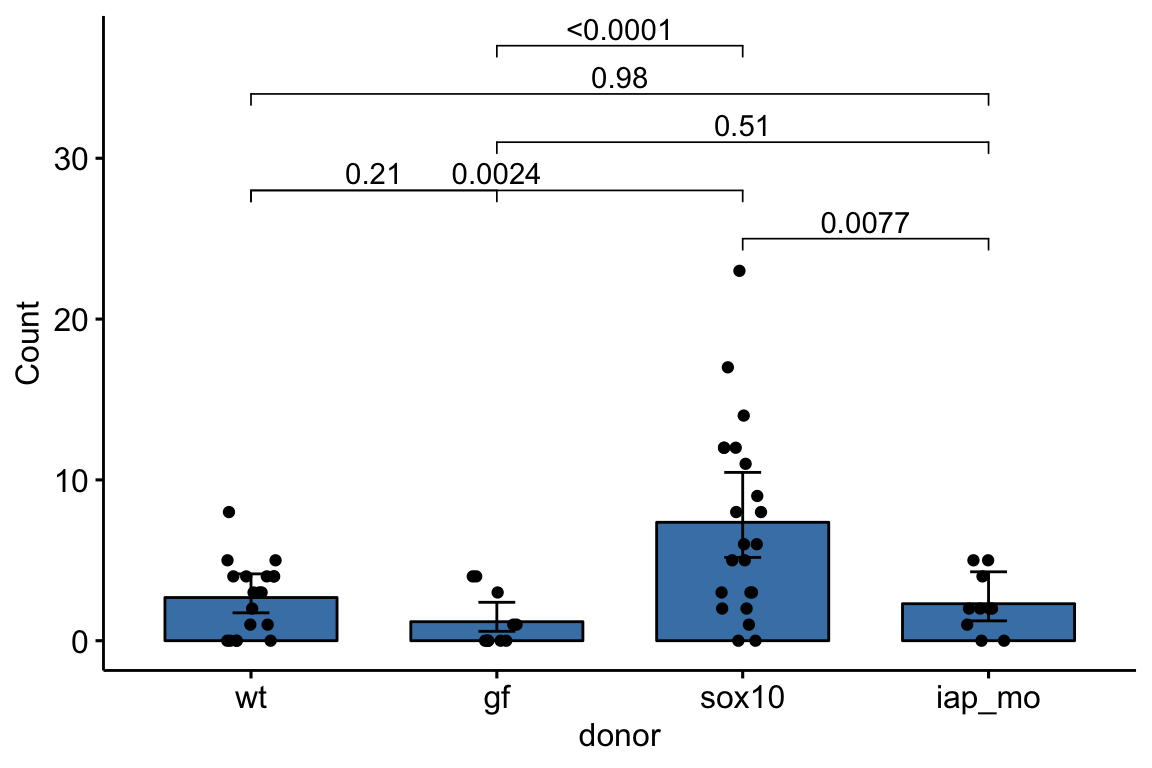
\includegraphics{Walker-elementary-statistical-modeling-draft_files/figure-latex/plots-means-1.pdf}
\caption{\label{fig:plots-means}Mean and error plot}
\end{figure}

Fig. \ref{fig:plots-means} plots the \emph{modeled} means, represented by the tops of the bars, the modeled 95\% confidence intervals of each mean, represented by the error bars, and the \emph{p}-values for all pairwise comparisons. What do I mean by \emph{modeled} means and error intervals?

\begin{enumerate}
\def\labelenumi{\arabic{enumi}.}
\tightlist
\item
  Modeled means and error intervals are estimated from the statistical model. Many published plots are of raw means and error intervals, meaning that the mean and error for each treatment level is computed only using the response measures in that treatment level.
\item
  A modeled mean will often be equal to the raw mean, but this will not always be the case, for example if there are covariates in the model (Chapter xxx).
\item
  Modeled error intervals are never the same as the raw error intervals, and are commonly conspicuously different. Almost always, we should plot modeled means and error intervals, since these represent the statistics that are relevant to inference.
\end{enumerate}

Fig. \ref{fig:plots-means} also plots the raw count data as ``jittered'' black dots. ``Showing the data'' is a pretty good feature of a plot because it allows the reader to get a sense of the underlying sample size and distribution including outliers, which can be used to mentally model check the published statistical analysis. For example, the jittered dots in Fig. \ref{fig:plots-means} suggest a \textbf{heterogeneity} of variances; specifically, the treatment level with the largest mean has a conspicuously higher variance. This pattern violates the assumptions of a general linear model and should raise a red flag to a reader if the researchers used a general linear model to analyze the data.

What a mean-and-error plot fails to show, at least directly, are the effects. To infer the effects from the plot, a reader must perform mental math -- either compute the difference or the ratio between pairs of means. This mental math is easy enough if the comparisons are between individual treatment levels but much harder if the comparisons are between pooled sets of treatment levels, for example in a factorial experimental design. The mental math that is excessively difficult is the reconstruction of some kind of error interval of the contrasts, for example the 95\% confidence intervals in Fig. \ref{plots-effect} and it is this interval that is necessary for a researcher to infer the range of biological consequences that are compatible with the experiment. The inclusion of the \emph{p}-values for all pairwise comparisons gives the significance level of these contrasts, but of the kinds of summary results that we could present (contrasts, error intervals, \emph{p}-values), the \emph{p}-values are the least informative.

\hypertarget{combining-effects-and-modeled-mean-and-ci-plots-an-effects-and-response-plot.}{%
\subsection{Combining Effects and Modeled mean and CI plots -- an Effects and response plot.}\label{combining-effects-and-modeled-mean-and-ci-plots-an-effects-and-response-plot.}}

If one wants to show both effects and the data, then these can be combined.

\begin{figure}
\centering
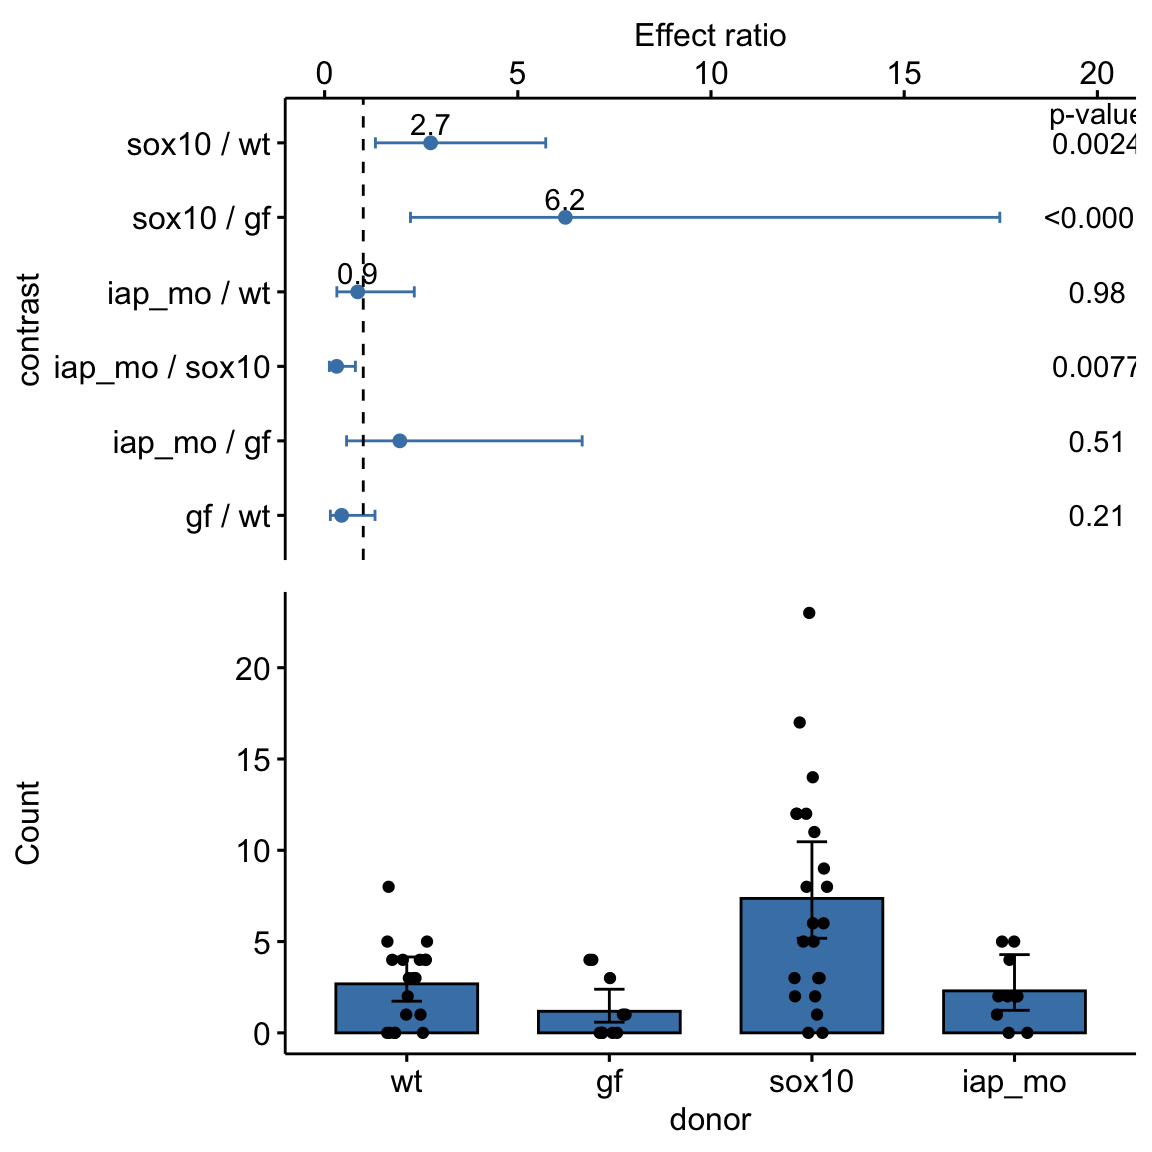
\includegraphics{Walker-elementary-statistical-modeling-draft_files/figure-latex/plots-harrellplot-1.pdf}
\caption{\label{fig:plots-harrellplot}A pretty good plot}
\end{figure}

If the means do not have any importance in understanding the results, the effects plot can be combined with some kind of a plot summarizing the distribution, such as a boxplot.

\begin{figure}
\centering
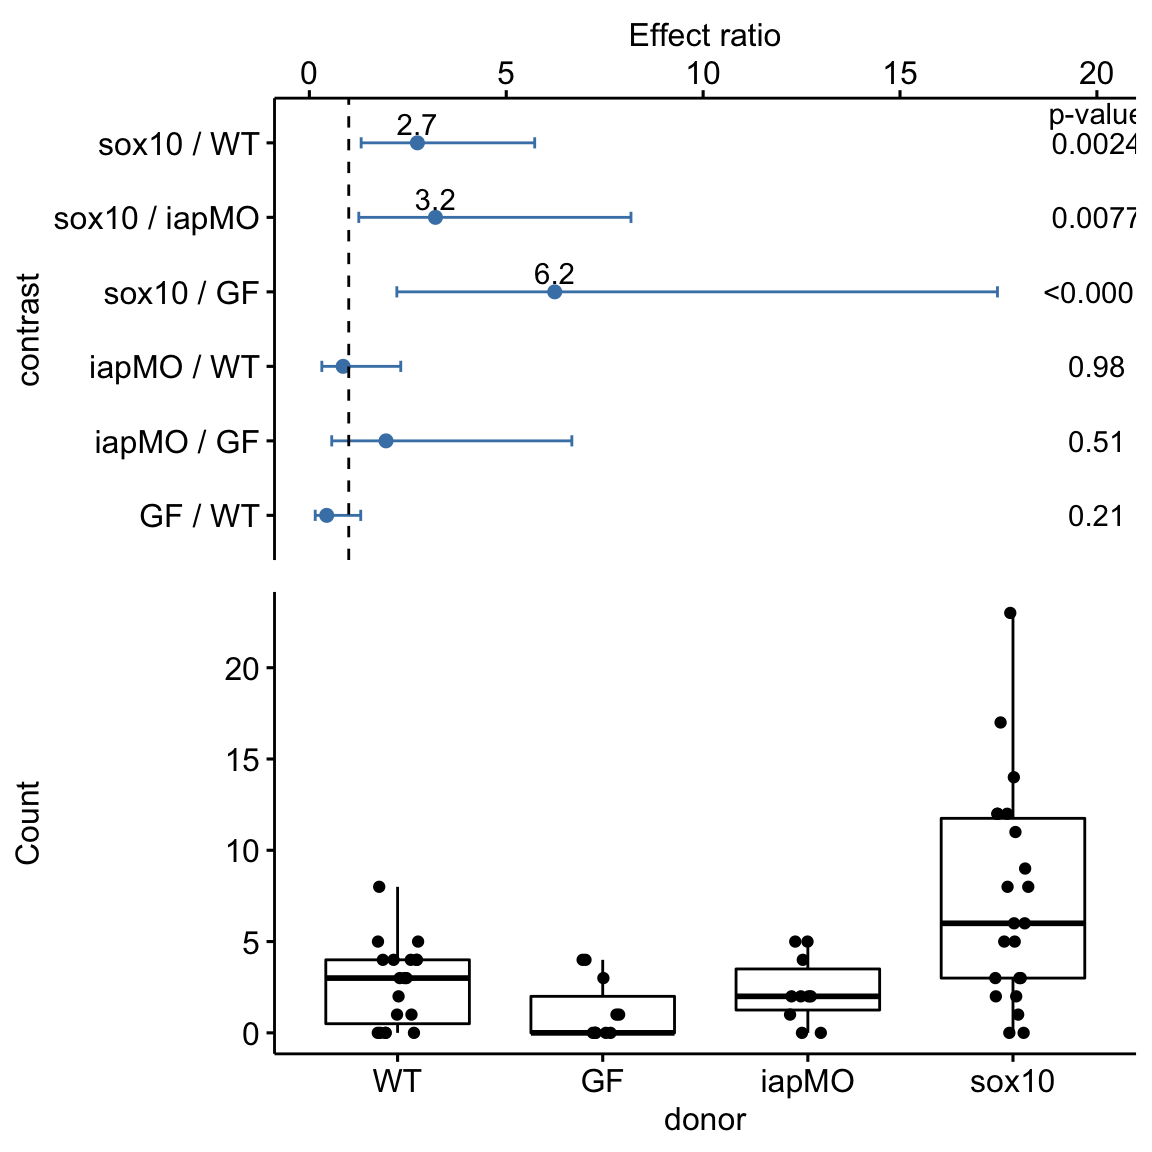
\includegraphics{Walker-elementary-statistical-modeling-draft_files/figure-latex/plots-harrelplot2-1.pdf}
\caption{\label{fig:plots-harrelplot2}Another pretty good plot}
\end{figure}

Regardless, the effects plot is the most important component as this is the illustration of the story a researcher wants to tell.

\hypertarget{some-comments-on-plot-components}{%
\section{Some comments on plot components}\label{some-comments-on-plot-components}}

\begin{enumerate}
\def\labelenumi{\arabic{enumi}.}
\tightlist
\item
  \textbf{Alternatives to barplots make good plots for the supplement, not the main paper}. A prominent trend over the last few years has been the replacement of bar plots with plots that ``show the data'', such as jitter plots or dot plots, or that show summaries of the distribution, such as box plots or violin plots. These plot types were developed for exploratory data analysis, not to communicate the results of experiments. All of these plots fail to communicate the results of the statistical model and, because of this, are inferior to an effects plot, and even a mean-and-error plot, if the mean and error are the modeled values. Box/Violoin/Dot/Jitter plots are a useful supplement to an effects plot, either combined with the effects plot as above, or as a supplementary figure.
\item
  Standard error bars, computed from the raw data, can have absurd implications. For example, I sometimes see standard error bars cross \(y=0\) for a response that cannot be negative, such as a count. Even if the standard error bar doesn't cross zero, it is common to see standard error bars that imply (but do not explicitly show) 95\% confidence intervals that cross zero, again for responses that cannot be negative. A standard error bar or confidence interval that crosses zero implies that negative means are compatible with the data. This is an absurd implication for responses that cannot have negative values (or are ``bounded by'' zero). Explicit or implicit error bars that cross zero are especially common for count responses with small means. \emph{If} a researcher plots confidence intervals, these should be computed using a method that avoids absurd implications, such methods include the bootstrap and generalized linear models.
\item
  \textbf{Stars add minimal value}. Many researchers add star symbols to a plot indicating the level of significance of a particular paired comparison. An uncommon, but better, alternative would be to add the actual p-value (as above). Adding a p-value (or stars) does communicate model results, and so adds value to a mean-and-error or box/violin/jitter plot. However, much more value would be added by simply reporting an effects plot or a combined effects-and-response plot.
\end{enumerate}

\hypertarget{working-in-r}{%
\section{Working in R}\label{working-in-r}}

A reasonable goal of any research project should be a script to generate the final plots entirely within the R environment and not rely on external drawing software to add finishing features. \href{https://ggplot2.tidyverse.org}{ggplot2} is one of the major plotting environments in R and the one that seems to have the strongest following, especially among new R users. ggplot2 has the ability to generate extremely personalized and finished plots. However, creating a plot with multiple layers (bars, lines, error intervals, raw data points, p-values, text annotations) can often require many hours of googling.

\href{https://cran.r-project.org/web/packages/ggpubr/index.html}{ggpubr} is an extension to ggplot2 (it calls ggplot2 functions under the hood) and provides many canned functions for producing the kinds of ggplots that are published in biological journals. With one line of script, a researcher can generate a publishable plot that is as good or better than many published plot.

\textbf{Here I show how to add custom (ggplot2) features to a ggpubr plot}

Throughout this book, ggpubr is used to create a basic plot and then additional features are added to the basic plot using ggplot2 functions.

\hypertarget{unpooled-se-bars-and-confidence-intervals}{%
\subsection{Unpooled SE bars and confidence intervals}\label{unpooled-se-bars-and-confidence-intervals}}

\texttt{ggplot2} and \texttt{ggpubr} default to unpooled error intervals (standard error bars and confidence intervals).

\begin{Shaded}
\begin{Highlighting}[]
\NormalTok{gg1 <-}\StringTok{ }\KeywordTok{ggbarplot}\NormalTok{(}\DataTypeTok{data =}\NormalTok{ exp2d,}
                 \DataTypeTok{x =} \StringTok{"donor"}\NormalTok{, }
                 \DataTypeTok{y =} \StringTok{"count"}\NormalTok{, }
                 \DataTypeTok{add =} \KeywordTok{c}\NormalTok{(}\StringTok{"mean_se"}\NormalTok{),}
                 \DataTypeTok{fill =} \StringTok{"steelblue"}
\NormalTok{)}
\NormalTok{gg2 <-}\StringTok{ }\KeywordTok{ggbarplot}\NormalTok{(}\DataTypeTok{data =}\NormalTok{ exp2d,}
                 \DataTypeTok{x =} \StringTok{"donor"}\NormalTok{, }
                 \DataTypeTok{y =} \StringTok{"count"}\NormalTok{, }
                 \DataTypeTok{add =} \KeywordTok{c}\NormalTok{(}\StringTok{"mean_ci"}\NormalTok{),}
                 \DataTypeTok{fill =} \StringTok{"steelblue"}
\NormalTok{)}
\KeywordTok{plot_grid}\NormalTok{(gg1, gg2, }\DataTypeTok{ncol=}\DecValTok{2}\NormalTok{, }\DataTypeTok{labels=}\StringTok{"AUTO"}\NormalTok{)}
\end{Highlighting}
\end{Shaded}

\begin{figure}
\centering
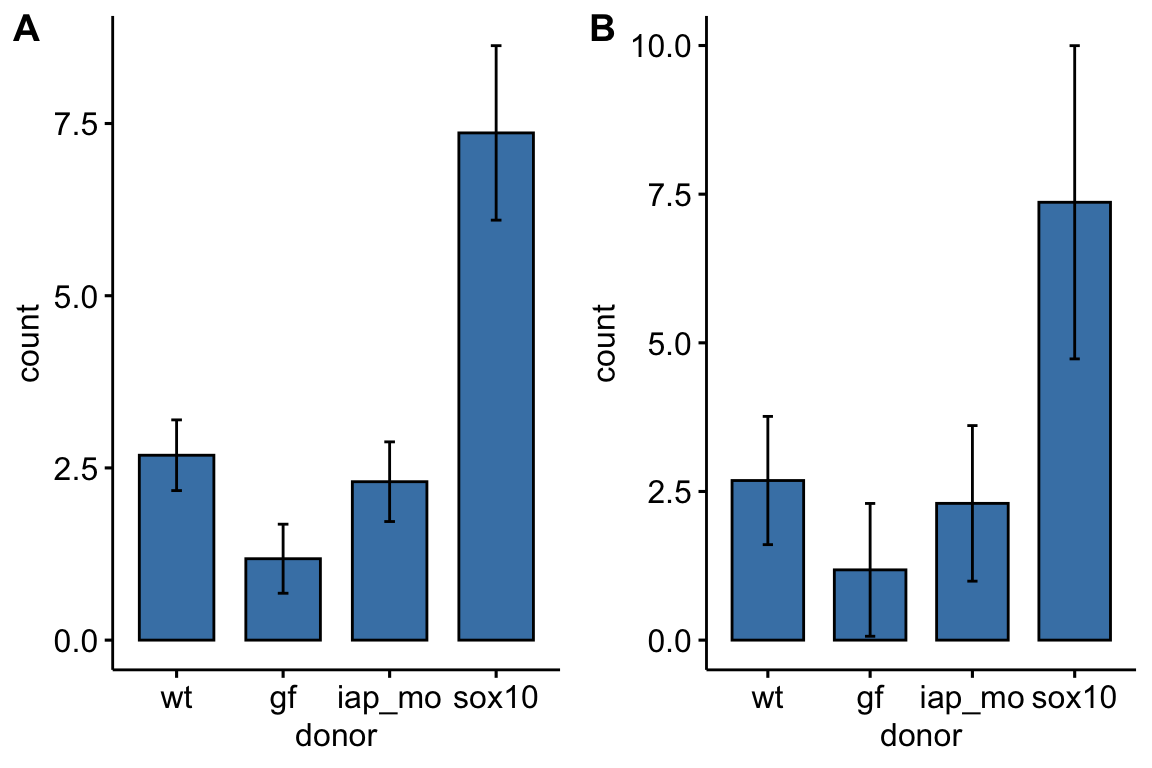
\includegraphics{Walker-elementary-statistical-modeling-draft_files/figure-latex/plots-unpooled-1.pdf}
\caption{\label{fig:plots-unpooled}(A) Mean and 1 SE error bar. (B) Mean and 95\% CI.}
\end{figure}

\hypertarget{adding-bootstrap-intervals}{%
\subsection{Adding bootstrap intervals}\label{adding-bootstrap-intervals}}

A bootstrap CI uses resamples of the data to estimate the interval and is a better choice than the default CI for data such as counts and proportions. The plot below uses ggpubr to create a stripchart of the data and the color of the data points are ``de-emphasized'' -- in order to emphasize the mean and CI -- by making them more transparent (using the argument \texttt{alpha}). \texttt{alpha} is added before the argument to add the mean in order to no de-emphasize the mean.

\begin{Shaded}
\begin{Highlighting}[]
\KeywordTok{set.seed}\NormalTok{(}\DecValTok{1}\NormalTok{)}
\NormalTok{gg.boot <-}\StringTok{ }\KeywordTok{ggstripchart}\NormalTok{(}\DataTypeTok{data=}\NormalTok{exp2d,}
                   \DataTypeTok{x =} \StringTok{"donor"}\NormalTok{, }
                   \DataTypeTok{y =} \StringTok{"count"}\NormalTok{, }
                   \DataTypeTok{alpha =} \FloatTok{0.4}\NormalTok{,}
                   \DataTypeTok{add =} \StringTok{"mean"}
\NormalTok{) }\OperatorTok{+}\StringTok{ }
\StringTok{  }\KeywordTok{stat_summary}\NormalTok{(}\DataTypeTok{fun.data =} \StringTok{"mean_cl_boot"}\NormalTok{, }
               \DataTypeTok{geom =} \StringTok{"errorbar"}\NormalTok{, }
               \DataTypeTok{width =} \FloatTok{0.1}\NormalTok{) }\OperatorTok{+}
\StringTok{  }\OtherTok{NULL}
\end{Highlighting}
\end{Shaded}

\begin{verbatim}
## Warning: `fun.y` is deprecated. Use `fun` instead.
\end{verbatim}

\begin{verbatim}
## Warning: `fun.ymin` is deprecated. Use `fun.min` instead.
\end{verbatim}

\begin{verbatim}
## Warning: `fun.ymax` is deprecated. Use `fun.max` instead.
\end{verbatim}

\begin{Shaded}
\begin{Highlighting}[]
\NormalTok{gg.boot}
\end{Highlighting}
\end{Shaded}

\begin{figure}
\centering
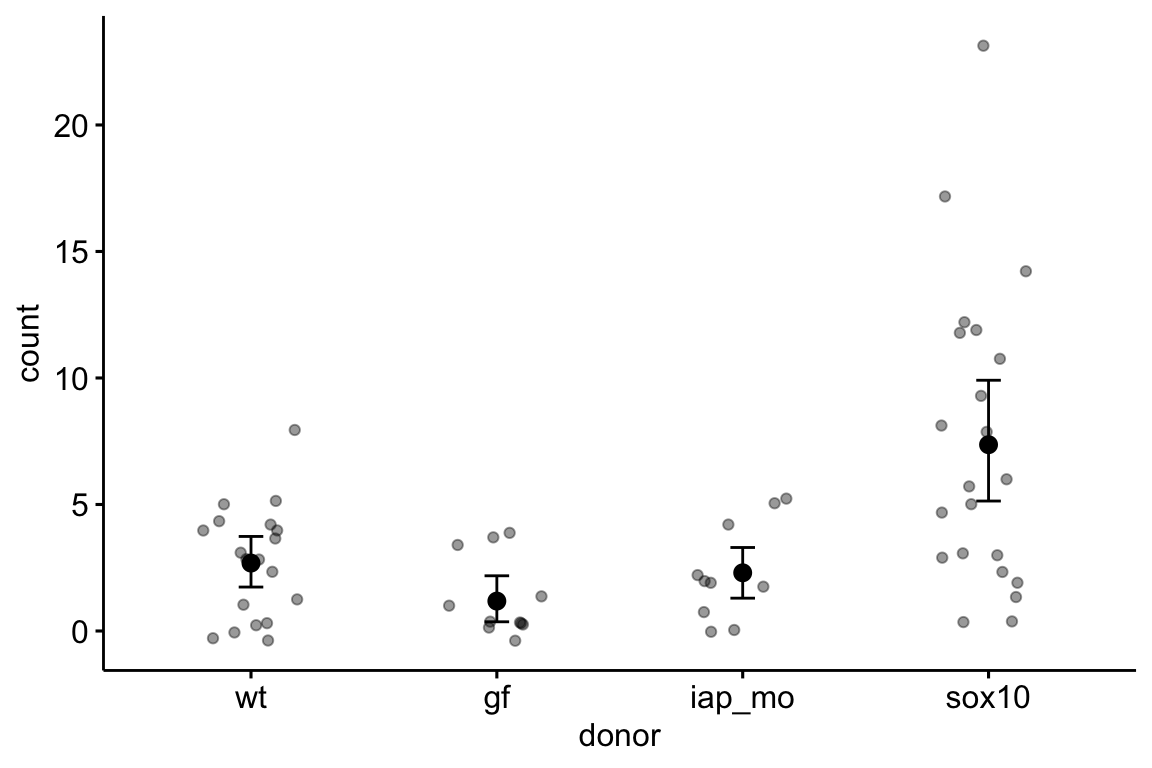
\includegraphics{Walker-elementary-statistical-modeling-draft_files/figure-latex/plot-boot-plot-1.pdf}
\caption{\label{fig:plot-boot-plot}Sample means with bootstrapped 95\% confidence intervals.}
\end{figure}

\hypertarget{adding-modeled-means-and-error-intervals}{%
\subsection{Adding modeled means and error intervals}\label{adding-modeled-means-and-error-intervals}}

This section is extremely important for implementing the work flow advocated in this text. The goal is to plot the modeled means with some sort of error interval, typically a confidence interval, \emph{and} to show the data or a summary of the data in a single plot. The procedure is

\begin{enumerate}
\def\labelenumi{\arabic{enumi}.}
\tightlist
\item
  fit the model
\item
  use the fit model to estimate the modeled means and confidence limits using \texttt{emmeans} from the \href{https://cran.r-project.org/web/packages/emmeans/index.html}{emmeans package}.
\item
  use the \texttt{emmean} object to estimate the contrasts of interests using the \texttt{contrast} function from emmeans.
\item
  Use the objects from steps 2 and 3 to plot the modeled means
\end{enumerate}

\textbf{Step 1: Fit the model}. A negative binomial, generalized linear model with log-link is fit to the count data.

\begin{Shaded}
\begin{Highlighting}[]
\NormalTok{m1 <-}\StringTok{ }\KeywordTok{glm.nb}\NormalTok{(count }\OperatorTok{~}\StringTok{ }\NormalTok{donor, }\DataTypeTok{data=}\NormalTok{exp2d)}
\KeywordTok{coef}\NormalTok{(}\KeywordTok{summary}\NormalTok{(m1))}
\end{Highlighting}
\end{Shaded}

\begin{verbatim}
##               Estimate Std. Error    z value     Pr(>|z|)
## (Intercept)  0.9873867  0.2229971  4.4278004 9.519895e-06
## donorgf     -0.8203326  0.4227008 -1.9406930 5.229553e-02
## donoriap_mo -0.1544775  0.3878578 -0.3982839 6.904209e-01
## donorsox10   1.0091672  0.2862047  3.5260325 4.218353e-04
\end{verbatim}

\begin{itemize}
\tightlist
\item
  The estimates and SE are on the \textbf{link scale}, which means they are in log-transformed space (or ``log space''). Exponentiate these with exp(x) to \textbf{backstransform} these to the the \textbf{response scale} which is the scale of the measurement (number of neutrophils).
\end{itemize}

\textbf{Step 2: Estimate the modeled means and confidence levels}. The second step is to pass the fit model object (m1) to \texttt{emmeans} to estimate the modeled means.

\begin{Shaded}
\begin{Highlighting}[]
\NormalTok{m1.emm <-}\StringTok{ }\KeywordTok{emmeans}\NormalTok{(m1, }\DataTypeTok{specs=}\StringTok{"donor"}\NormalTok{, }\DataTypeTok{type=}\StringTok{"response"}\NormalTok{)}
\NormalTok{m1.emm}
\end{Highlighting}
\end{Shaded}

\begin{verbatim}
##  donor  response    SE  df asymp.LCL asymp.UCL
##  wt         2.68 0.599 Inf     1.734      4.16
##  gf         1.18 0.424 Inf     0.585      2.39
##  iap_mo     2.30 0.730 Inf     1.235      4.28
##  sox10      7.36 1.321 Inf     5.181     10.47
## 
## Confidence level used: 0.95 
## Intervals are back-transformed from the log scale
\end{verbatim}

\begin{itemize}
\tightlist
\item
  We specify the means that we want to estimate with ``specs =''. Here, we want to estimate the means of the levels of \(donor\).
\item
  Because the linear predictor of the model is on the log scale, we use the ``type'' argument to specify that we want the means to be backtransformed to the \textbf{response scale}, which is the scale of the measurement (number of cells)
\item
  It can be useful to convert the emmeans table m1.emm to a data.table (or data.frame or tibble) using \texttt{m1.emm\ \textless{}-\ data.table(m1.emm)}. \textbf{Bug alert} If you do this, the object cannot be passed to the next step, the \texttt{contrast} function. So if you want the emmeans table as a data.table, assign it to a different name, for example \texttt{m1.emm\_dt\ \textless{}-\ data.table(m1.emm)}.
\end{itemize}

\textbf{Step 3: Compute the contrasts, with p-values and confidence levels}. Contrasts among levels, or combinations of levels, are computed by passing the emmeans object (m1.emm) to the \texttt{contrast} function.

\begin{Shaded}
\begin{Highlighting}[]
\NormalTok{m1.pairs <-}\StringTok{ }\KeywordTok{contrast}\NormalTok{(m1.emm, }\DataTypeTok{method=}\StringTok{"revpairwise"}\NormalTok{, }\DataTypeTok{adjust=}\StringTok{"none"}\NormalTok{) }\OperatorTok
\StringTok{  }\KeywordTok{summary}\NormalTok{(}\DataTypeTok{infer=}\KeywordTok{c}\NormalTok{(}\OtherTok{TRUE}\NormalTok{, }\OtherTok{TRUE}\NormalTok{))}
\NormalTok{m1.pairs}
\end{Highlighting}
\end{Shaded}

\begin{verbatim}
##  contrast       ratio    SE  df asymp.LCL asymp.UCL z.ratio p.value
##  gf / wt        0.440 0.186 Inf     0.192      1.01 -1.941  0.0523 
##  iap_mo / wt    0.857 0.332 Inf     0.401      1.83 -0.398  0.6904 
##  iap_mo / gf    1.946 0.933 Inf     0.761      4.98  1.389  0.1647 
##  sox10 / wt     2.743 0.785 Inf     1.566      4.81  3.526  0.0004 
##  sox10 / gf     6.231 2.501 Inf     2.837     13.68  4.558  <.0001 
##  sox10 / iap_mo 3.202 1.167 Inf     1.567      6.54  3.192  0.0014 
## 
## Confidence level used: 0.95 
## Intervals are back-transformed from the log scale 
## Tests are performed on the log scale
\end{verbatim}

\begin{itemize}
\tightlist
\item
  Here, we set ``method'' to ``revpairwise'' in order to compute contrasts among all pairs of levels of \(donor\). There are \(m = 4\) levels and so \(m(m-1)/2 = 6\) pairwise contrasts. ``revpairwise'' is used instead of ``pairwise'' because the former sets the direction of the contrasts that include the reference as non-reference level minus reference level.
\item
  I use the ``adjust'' argument to specify no \emph{p}-value adjustment for multiple tests.
\item
  the contrast object is then piped (\%\textgreater\%) to the summary function, where I pass to the argument ``infer'', that I want both the confidence intervals (the first TRUE) and \emph{p}-values (the second TRUE)
\item
  this step isn't necessary if we were plotting only modeled means and CIs but 1) we almost always want contrasts with a fit model and so that is done here as part of the uninterrupted work flow that this book advocates and 2) we do use the \emph{p}-values and CIs from this table (m1.pairs) in the final plot below.
\item
  \textbf{Bug alert} again, the emmeans table m1.emm must be passed to \texttt{contrast} as an emmeans object. If you have converted this object to a data.table, you will get an error. See the last note in Step 2.
\end{itemize}

\textbf{Step 4: Plot the modeled means and 95\% error intervals}.

The code below first creates the stripchart using the ggpubr function and then adds the confidence intervals using \texttt{geom\_errorbar} and means using \texttt{geom\_point}. The stripchart uses the data in the exp2d data.table. The errorbar and mean use the values in m1.emm object created by the \texttt{emmeans} function. The \texttt{geom\_errorbar} and \texttt{geom\_point} functions require an ``aesthetic'' to tell ggplot which column contains the y values of the points to plot (the ``x'' values are still in the column ``donor'', which is a column in both the exp2d data.table and m1.emm). The name of the column containing the ``y'' values in m1.emm is ``response''.

\begin{Shaded}
\begin{Highlighting}[]
\KeywordTok{set.seed}\NormalTok{(}\DecValTok{1}\NormalTok{)}
\NormalTok{gg.nb <-}\StringTok{ }\KeywordTok{ggstripchart}\NormalTok{(}\DataTypeTok{data=}\NormalTok{exp2d,}
                 \DataTypeTok{x=}\StringTok{"donor"}\NormalTok{, }
                 \DataTypeTok{y=}\StringTok{"count"}\NormalTok{,}
                 \DataTypeTok{alpha =} \FloatTok{0.4}\NormalTok{) }\OperatorTok{+}
\StringTok{  }\KeywordTok{ylab}\NormalTok{(}\StringTok{"Neutrophil count"}\NormalTok{) }\OperatorTok{+}
\StringTok{  }\KeywordTok{geom_errorbar}\NormalTok{(}\DataTypeTok{data=}\KeywordTok{summary}\NormalTok{(m1.emm), }
                \KeywordTok{aes}\NormalTok{(}\DataTypeTok{y=}\NormalTok{response,}
                    \DataTypeTok{ymin=}\NormalTok{asymp.LCL, }
                    \DataTypeTok{ymax=}\NormalTok{asymp.UCL), }
                \DataTypeTok{width=}\FloatTok{0.1}\NormalTok{) }\OperatorTok{+}
\StringTok{  }\KeywordTok{geom_point}\NormalTok{(}\DataTypeTok{data=}\KeywordTok{summary}\NormalTok{(m1.emm), }
                \KeywordTok{aes}\NormalTok{(}\DataTypeTok{y=}\NormalTok{response), }
                \DataTypeTok{size=}\DecValTok{2}\NormalTok{) }\OperatorTok{+}
\StringTok{  }\OtherTok{NULL}

\NormalTok{gg.nb}
\end{Highlighting}
\end{Shaded}

\begin{figure}
\centering
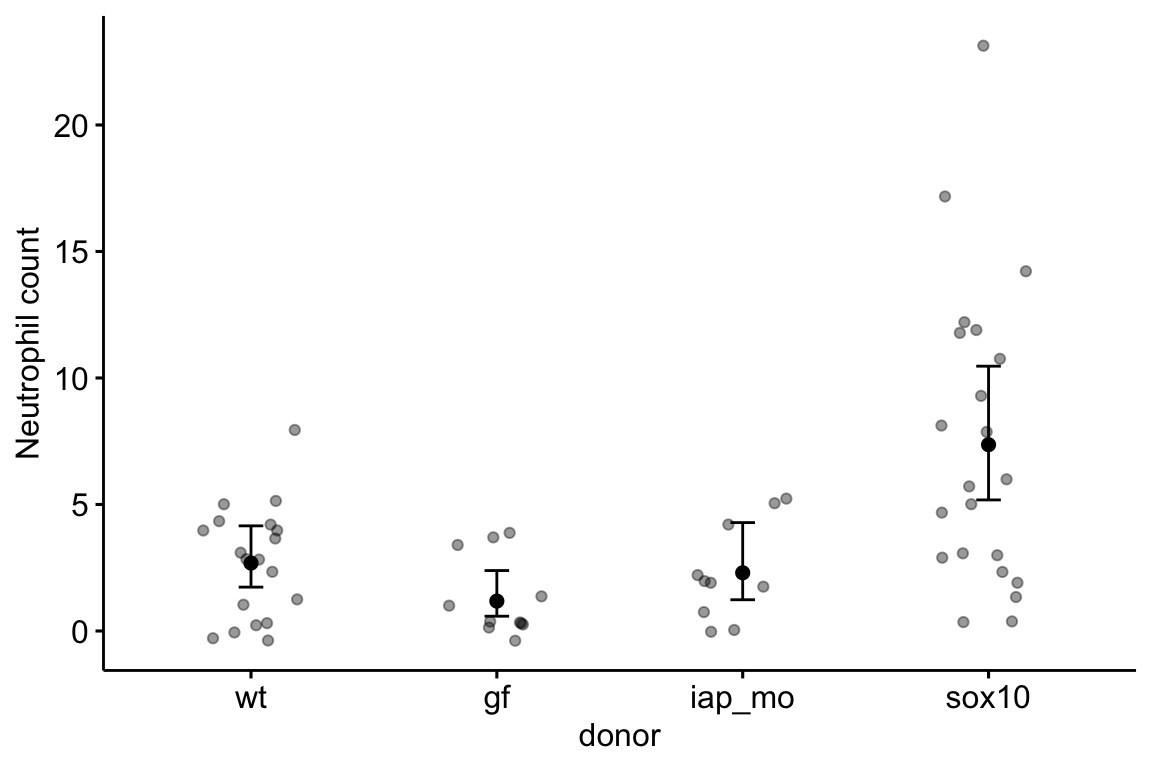
\includegraphics{Walker-elementary-statistical-modeling-draft_files/figure-latex/plot-nb-plot-1.pdf}
\caption{\label{fig:plot-nb-plot}Modeled means and 95\% confidence interval computed from a negative binomial generalized linear model.}
\end{figure}

Some notes on the plot code

\begin{itemize}
\tightlist
\item
  A column name passed to a \texttt{ggpubr} function must be in quotes but a column name passed to a \texttt{ggplot2} function cannot be in quotes
\item
  \textbf{Bug alert}. The data passed to ggplot2 must be a data.frame. In order for the ggplot2 functions to use the m1.emm object, the object has to be passed as \texttt{summary(m1.emm)}.
\item
  \textbf{Bug alert}. Because the m1.emm table does not have a column named ``count'', which is the ``y'' column specified in \texttt{ggstripchart}, you must supply a new ``y'' column name to the \texttt{aes} function of \texttt{geom\_errorbar} and \texttt{geom\_point}. This is the name of the column in the emmeans table containing the modeled means. In m1.emm, this name is ``response'' but it can take different names in different emmeans tables, depending on the fit model.
\end{itemize}

\hypertarget{adding-p-values}{%
\subsection{Adding p-values}\label{adding-p-values}}

In this section, I show how to add \emph{p}-values to a ggpubr plot using \texttt{stat\_compare\_means}. Because this function has only a limited set of models that can be used to compute the \emph{p}-values, I don't find it very useful and instead recommend adding custom \emph{p}-values from the fit model (or from a permutation test) using the method in the next section.

For this example, a ``t.test'' is used to compute the p-values. The mean and error are the sample-based estimates because these, and not the modeled estimates, are consistent with the t-test \emph{p}-values.

\begin{Shaded}
\begin{Highlighting}[]
\NormalTok{compare_list <-}\StringTok{ }\KeywordTok{list}\NormalTok{(}\KeywordTok{c}\NormalTok{(}\StringTok{"sox10"}\NormalTok{, }\StringTok{"iap_mo"}\NormalTok{), }\KeywordTok{c}\NormalTok{(}\StringTok{"sox10"}\NormalTok{, }\StringTok{"gf"}\NormalTok{), }\KeywordTok{c}\NormalTok{(}\StringTok{"sox10"}\NormalTok{, }\StringTok{"wt"}\NormalTok{))}

\NormalTok{gg.sample <-}\StringTok{ }\KeywordTok{ggstripchart}\NormalTok{(}\DataTypeTok{data=}\NormalTok{exp2d,}
          \DataTypeTok{x=}\StringTok{"donor"}\NormalTok{, }
          \DataTypeTok{y=}\StringTok{"count"}\NormalTok{,}
          \DataTypeTok{alpha =} \FloatTok{0.4}\NormalTok{,}
          \DataTypeTok{add=}\KeywordTok{c}\NormalTok{(}\StringTok{"mean_ci"}\NormalTok{)) }\OperatorTok{+}
\StringTok{  }\KeywordTok{stat_compare_means}\NormalTok{(}\DataTypeTok{method =} \StringTok{"t.test"}\NormalTok{, }\DataTypeTok{comparisons=}\NormalTok{compare_list) }\OperatorTok{+}
\StringTok{  }\KeywordTok{ylab}\NormalTok{(}\StringTok{"Neutrophil count"}\NormalTok{) }\OperatorTok{+}
\StringTok{  }\OtherTok{NULL}

\NormalTok{gg.sample}
\end{Highlighting}
\end{Shaded}

\begin{figure}
\centering
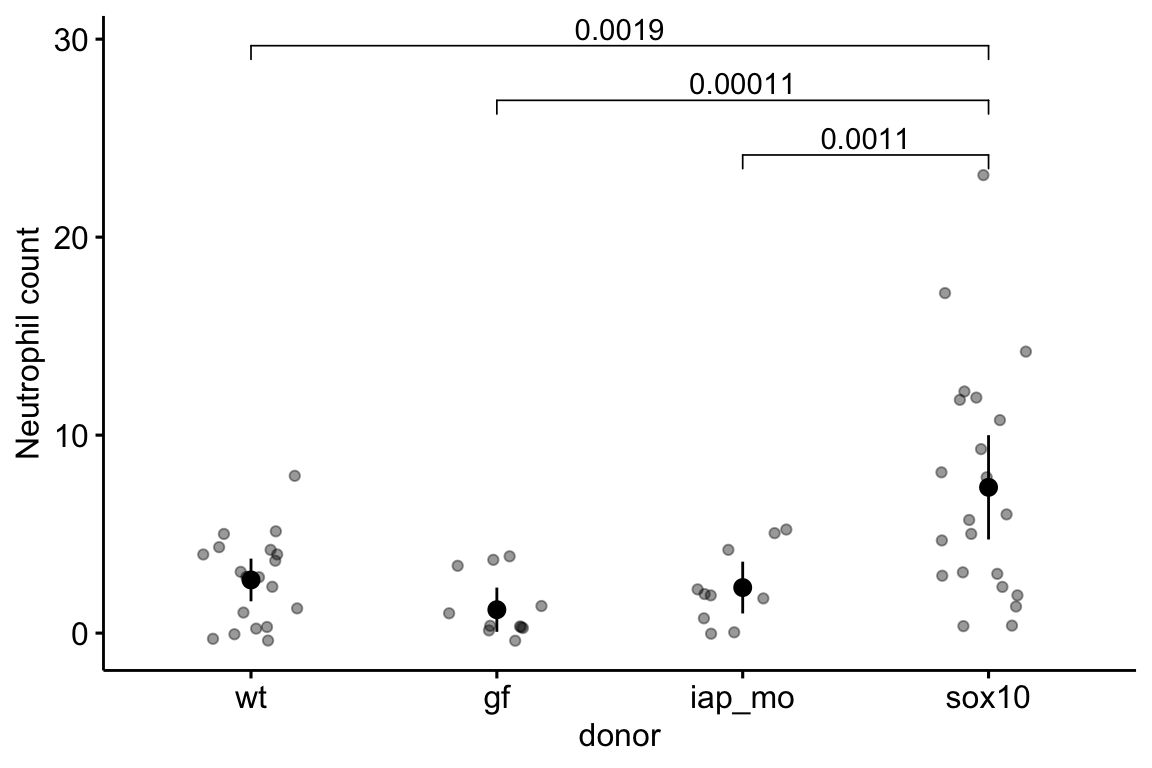
\includegraphics{Walker-elementary-statistical-modeling-draft_files/figure-latex/plot-p-values-1.pdf}
\caption{\label{fig:plot-p-values}t-test p-values for the plot of sample means and CIs. The p-values were computed using ggpubr's function stat\_compare\_means.}
\end{figure}

Notes on the code

\begin{itemize}
\item
  The pairs to compare with a \emph{p}-value are specified with \texttt{comparison\ =}. The order of the pairs in the list function determine the order plotted from bottom (lowest on the y-axis) to top (highest on the y-axis).
\item
  \textbf{It is important to know what exactly is being computed when analyzing data and reporting results} and ``t test'' is not sufficient to know this. The t-test could be the classic t-test or a Welch test. In this example, there are multiple comparisons and the standard error of the test statistic could be the pooled estimate from the linear model, or a pairwise estimate computed separately for each pair. And, given the multiple comparisons, the p-values could be adjusted or not. These kinds of questions can be checked with a function's help page. \texttt{?stat\_compare\_means} doesn't answer these questions but suggests \texttt{compare\_means}, which also doesn't answer these questions. The script below has checks to see what p-values the function is returning. Run it in your session by changing the value of check\_it to TRUE.
\end{itemize}

\begin{Shaded}
\begin{Highlighting}[]
\CommentTok{# checks on the p-value}
\CommentTok{# t-tests using SE pooled over all four groups}
\NormalTok{check_it <-}\StringTok{ }\OtherTok{FALSE}
\ControlFlowTok{if}\NormalTok{(check_it}\OperatorTok{==}\OtherTok{TRUE}\NormalTok{)\{}
\NormalTok{  m1.lm <-}\StringTok{ }\KeywordTok{lm}\NormalTok{(count}\OperatorTok{~}\NormalTok{donor, }\DataTypeTok{data=}\NormalTok{exp2d)}
\NormalTok{  m1.lm.emm <-}\StringTok{ }\KeywordTok{emmeans}\NormalTok{(m1.lm, }\DataTypeTok{specs=}\StringTok{"donor"}\NormalTok{)}
  \KeywordTok{contrast}\NormalTok{(m1.lm.emm, }\DataTypeTok{method=}\StringTok{"trt.vs.ctrl"}\NormalTok{, }\DataTypeTok{ref=}\DecValTok{4}\NormalTok{, }\DataTypeTok{adjust=}\StringTok{"none"}\NormalTok{) }\CommentTok{# pooled SD}
  
  \KeywordTok{pairwise.t.test}\NormalTok{(exp2d}\OperatorTok{$}\NormalTok{count, exp2d}\OperatorTok{$}\NormalTok{donor, }\DataTypeTok{p.adjust.method=}\StringTok{"none"}\NormalTok{, }\DataTypeTok{pool.sd=}\OtherTok{FALSE}\NormalTok{) }\CommentTok{# non-pooled SD}
  \CommentTok{# compare}
  \KeywordTok{t.test}\NormalTok{(count}\OperatorTok{~}\NormalTok{donor, }\DataTypeTok{data=}\NormalTok{exp2d[donor}\OperatorTok{==}\StringTok{"wt"} \OperatorTok{|}\StringTok{ }\NormalTok{donor}\OperatorTok{==}\StringTok{"sox10"}\NormalTok{]) }\CommentTok{# matches, this is Welch t}
  \KeywordTok{t.test}\NormalTok{(count}\OperatorTok{~}\NormalTok{donor, }\DataTypeTok{data=}\NormalTok{exp2d[donor}\OperatorTok{==}\StringTok{"wt"} \OperatorTok{|}\StringTok{ }\NormalTok{donor}\OperatorTok{==}\StringTok{"sox10"}\NormalTok{], }\DataTypeTok{var.equal=}\OtherTok{TRUE}\NormalTok{)}
\NormalTok{\}}
\end{Highlighting}
\end{Shaded}

So, the \emph{p}-values returned by \texttt{stat\_compare\_means(method="t.test")} are computed from independent (not pooled over the four groups) Welch t-tests.

\hypertarget{adding-custom-p-values}{%
\subsection{Adding custom p-values}\label{adding-custom-p-values}}

If we want to add permutation \emph{p}-values to the plot with bootstrapped CIs (\ref{fig:plot-boot-plot} or add \emph{p}-values from the generalized linear model to the plot of modeled means and CIs (\ref{fig:plot-nb-plot}, we need to use the function \texttt{stat\_pvalue\_manual} from the ggpubr package. In order to implement this, we need to add a step to the work flow path above

\textbf{Step 5: Add group columns and a column of formatted p-values to the contrast table}

The \texttt{stat\_pvalue\_manual} function needs to read a data frame with a columns labeled ``group1'' and ``group2'' that contain the pairs of levels to compare with a plotted p-value and a column ``p'' containing the nicely formatted p-values to add to the plot. There is no R function to create this table, but here is a script to add these to the contrast object returned by the \texttt{contrast} function of emmeans. In this example, I use m1.pairs from above and add the p-values to the plot of modeled means and CIs (\ref{fig:plot-nb-plot}.

First, we need these functions. Run these two lines to define the functions \texttt{odd} and \texttt{even}

\begin{Shaded}
\begin{Highlighting}[]
\NormalTok{odd <-}\StringTok{ }\ControlFlowTok{function}\NormalTok{(x) x}\OperatorTok\DecValTok{2} \OperatorTok{!=}\StringTok{ }\DecValTok{0}
\NormalTok{even <-}\StringTok{ }\ControlFlowTok{function}\NormalTok{(x) x}\OperatorTok\DecValTok{2} \OperatorTok{==}\StringTok{ }\DecValTok{0}
\end{Highlighting}
\end{Shaded}

Second, we need to use these functions to add the columns. There are several R packages that provide functions to format \emph{p}-values. Here, I use the function \texttt{pvalString} from the \href{https://www.rdocumentation.org/packages/lazyWeave/versions/3.0.2/topics/pvalString}{lazyWeave} package. This script also uses \texttt{str\_split} from the package \href{https://cran.r-project.org/web/packages/stringr/index.html}{stringr}.

\begin{Shaded}
\begin{Highlighting}[]
\CommentTok{# convert m1.pairs to a data.table and assign to a new object, in order to}
\CommentTok{# keep a clean copy of m1.pairs}
\NormalTok{m1.pvalues <-}\StringTok{ }\KeywordTok{data.table}\NormalTok{(m1.pairs)}

\CommentTok{# if the linear model is from a glm with log link, use this}
\NormalTok{groups <-}\StringTok{ }\KeywordTok{unlist}\NormalTok{(}\KeywordTok{str_split}\NormalTok{(m1.pvalues}\OperatorTok{$}\NormalTok{contrast, }\StringTok{" / "}\NormalTok{))}
\CommentTok{# add the group1 and group 2 columns}
\NormalTok{m1.pvalues[, group1 }\OperatorTok{:}\ErrorTok{=}\StringTok{ }\NormalTok{groups[}\KeywordTok{odd}\NormalTok{(}\DecValTok{1}\OperatorTok{:}\KeywordTok{length}\NormalTok{(groups))]]}
\NormalTok{m1.pvalues[, group2 }\OperatorTok{:}\ErrorTok{=}\StringTok{ }\NormalTok{groups[}\KeywordTok{even}\NormalTok{(}\DecValTok{1}\OperatorTok{:}\KeywordTok{length}\NormalTok{(groups))]]}

\CommentTok{# create a column of nicely formatted p-values for display.}
\NormalTok{m1.pvalues[, p }\OperatorTok{:}\ErrorTok{=}\StringTok{ }\KeywordTok{pvalString}\NormalTok{(p.value)]}
\end{Highlighting}
\end{Shaded}

\textbf{Bug alert} notes on the script to build the p-value table, if you don't want your code to fail.

\begin{itemize}
\tightlist
\item
  The script to extract the pair of group labels \texttt{str\_split(m1.pvalues\$contrast,\ "\ /\ "))} has to be written so that the characters within the quotes matches the characters separating the groups in the ``contrast'' column of the contrast table (here, m1.pairs). This will typically be either a space-minus-space or a space-slash-space. If the model fit is \texttt{lm} and the response is not transformed, then the correct code is \texttt{str\_split(m1.pvalues\$contrast,\ "\ -\ "))}. Regardless, look at the table to check.
\item
  In step 3 above, we took the contrast table object and passed it to the function \texttt{summary}, which converts the contrast table object to a data.frame. If we had skipped this step, \texttt{data.table(m1.pairs)} would fail. Instead, we'd have to use \texttt{data.table(summary(m1.pairs))}.
\end{itemize}

Now we can add the p-value to the ggplot object gg.nb created above. This is the beauty of a ggplot object (including those created by ggpubr), we can just keep adding stuff to it.

\begin{Shaded}
\begin{Highlighting}[]
\NormalTok{gg.nb <-}\StringTok{ }\NormalTok{gg.nb }\OperatorTok{+}
\StringTok{    }\KeywordTok{stat_pvalue_manual}\NormalTok{(m1.pvalues[}\DecValTok{4}\OperatorTok{:}\DecValTok{6}\NormalTok{,], }\CommentTok{# only show sox effects}
                           \DataTypeTok{label =} \StringTok{"p"}\NormalTok{, }
                           \DataTypeTok{y.position=}\KeywordTok{c}\NormalTok{(}\DecValTok{31}\NormalTok{, }\DecValTok{28}\NormalTok{, }\DecValTok{25}\NormalTok{)) }\OperatorTok{+}
\StringTok{  }\OtherTok{NULL}

\NormalTok{gg.nb}
\end{Highlighting}
\end{Shaded}

\begin{figure}
\centering
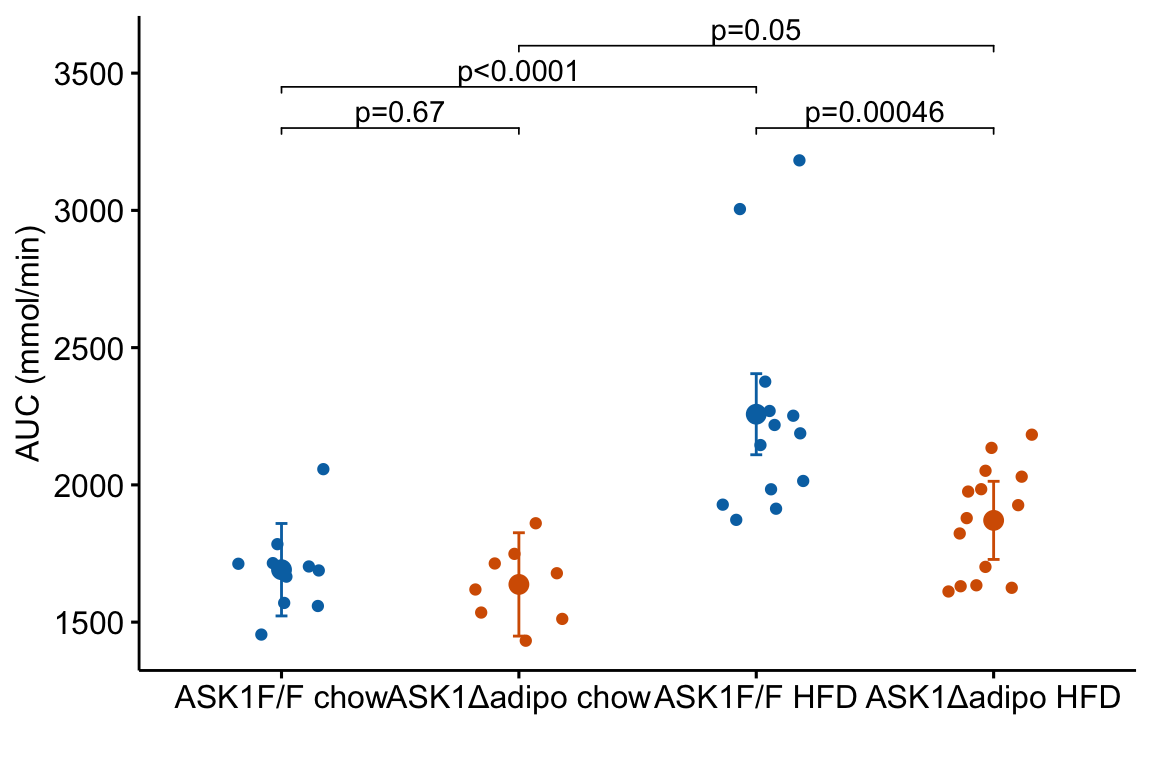
\includegraphics{Walker-elementary-statistical-modeling-draft_files/figure-latex/plot-manual-p-values-1.pdf}
\caption{\label{fig:plot-manual-p-values}Effects and means plot. Top panel: Effects (top panel) of treatments on neutrophil count. Bottom panel: modeled means of treatment levels with 95\% confidence intervals.}
\end{figure}

Notes on adding manual \emph{p}-values to the plot:

\begin{itemize}
\tightlist
\item
  The pairs of groups to compare are specified by indexing the rows of m1.pvalues. Above, I limit the comparisons to those in rows 4-6. If I wanted to specify non-continous rows, I could use something like \texttt{m1.pvalues{[}c(1,3,5),{]}}, for example.
\item
  The most manual part of adding manual p-values is setting the position for the brackets using the ``position'' argument. The values in this argument are the y-coordinates of the brackets. This may take some trial-and-error to position the brackets satisfactorily.
\end{itemize}

\hypertarget{modeled-error-intervals-of-the-effect}{%
\subsubsection{Modeled error intervals of the effect}\label{modeled-error-intervals-of-the-effect}}

For the plot of effects, we use table of contrasts m1.pairs as the data.

\begin{Shaded}
\begin{Highlighting}[]
\NormalTok{gg.effects <-}\StringTok{ }\KeywordTok{ggdotplot}\NormalTok{(}\DataTypeTok{data =}\NormalTok{ m1.pairs,}
                        \DataTypeTok{x=}\StringTok{"contrast"}\NormalTok{, }
                        \DataTypeTok{y=}\StringTok{"ratio"}\NormalTok{, }
                        \DataTypeTok{color =} \StringTok{"steelblue"}\NormalTok{,}
                        \DataTypeTok{fill =} \StringTok{"steelblue"}\NormalTok{,}
                        \DataTypeTok{size=}\FloatTok{0.5}\NormalTok{) }\OperatorTok{+}
\StringTok{  }
\StringTok{  }\KeywordTok{geom_errorbar}\NormalTok{(}\KeywordTok{aes}\NormalTok{(}\DataTypeTok{x=}\NormalTok{contrast, }
                    \DataTypeTok{ymin=}\NormalTok{asymp.LCL, }
                    \DataTypeTok{ymax=}\NormalTok{asymp.UCL),}
                \DataTypeTok{width=}\FloatTok{0.15}\NormalTok{, }
                \DataTypeTok{color=}\StringTok{"steelblue"}\NormalTok{) }\OperatorTok{+}
\StringTok{  }\KeywordTok{ylab}\NormalTok{(}\StringTok{"Effect ratio"}\NormalTok{) }\OperatorTok{+}
\StringTok{  }\KeywordTok{geom_hline}\NormalTok{(}\DataTypeTok{yintercept=}\DecValTok{1}\NormalTok{, }\DataTypeTok{linetype =} \DecValTok{2}\NormalTok{) }\OperatorTok{+}
\StringTok{  }\KeywordTok{coord_flip}\NormalTok{() }\OperatorTok{+}\StringTok{ }
\StringTok{  }
\StringTok{  }\OtherTok{NULL}

\NormalTok{gg.effects}
\end{Highlighting}
\end{Shaded}

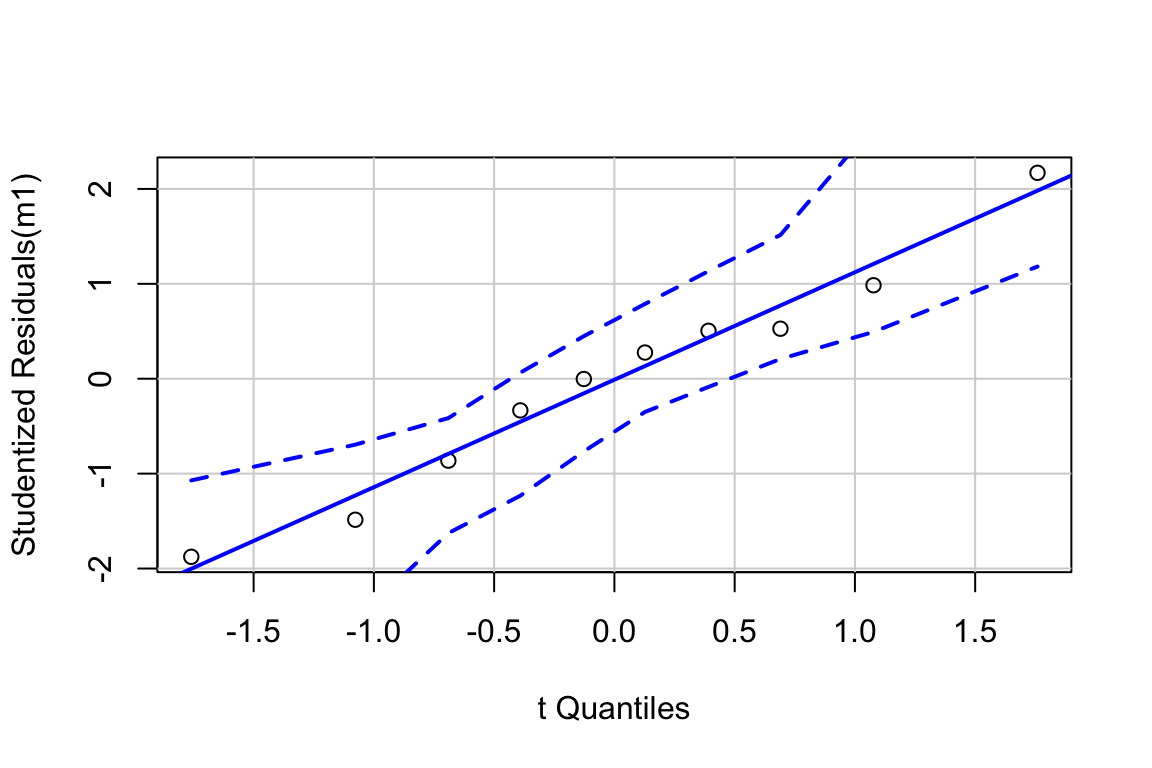
\includegraphics{Walker-elementary-statistical-modeling-draft_files/figure-latex/unnamed-chunk-85-1.pdf}

\hypertarget{combining-effects-and-response-plots}{%
\subsubsection{Combining effects and response plots}\label{combining-effects-and-response-plots}}

The ggplots are combined using \texttt{plot\_grid} from the package \href{https://cran.r-project.org/web/packages/cowplot/vignettes/introduction.html}{cowplot}

\begin{Shaded}
\begin{Highlighting}[]
\NormalTok{gg.effects <-}\StringTok{ }\NormalTok{gg.effects }\OperatorTok{+}\StringTok{ }\KeywordTok{scale_y_continuous}\NormalTok{(}\DataTypeTok{position=}\StringTok{"right"}\NormalTok{)}
\KeywordTok{plot_grid}\NormalTok{(gg.effects, gg.nb, }\DataTypeTok{nrow=}\DecValTok{2}\NormalTok{, }\DataTypeTok{align =} \StringTok{"v"}\NormalTok{, }\DataTypeTok{rel_heights =} \KeywordTok{c}\NormalTok{(}\DecValTok{1}\NormalTok{, }\DecValTok{2}\NormalTok{))}
\end{Highlighting}
\end{Shaded}

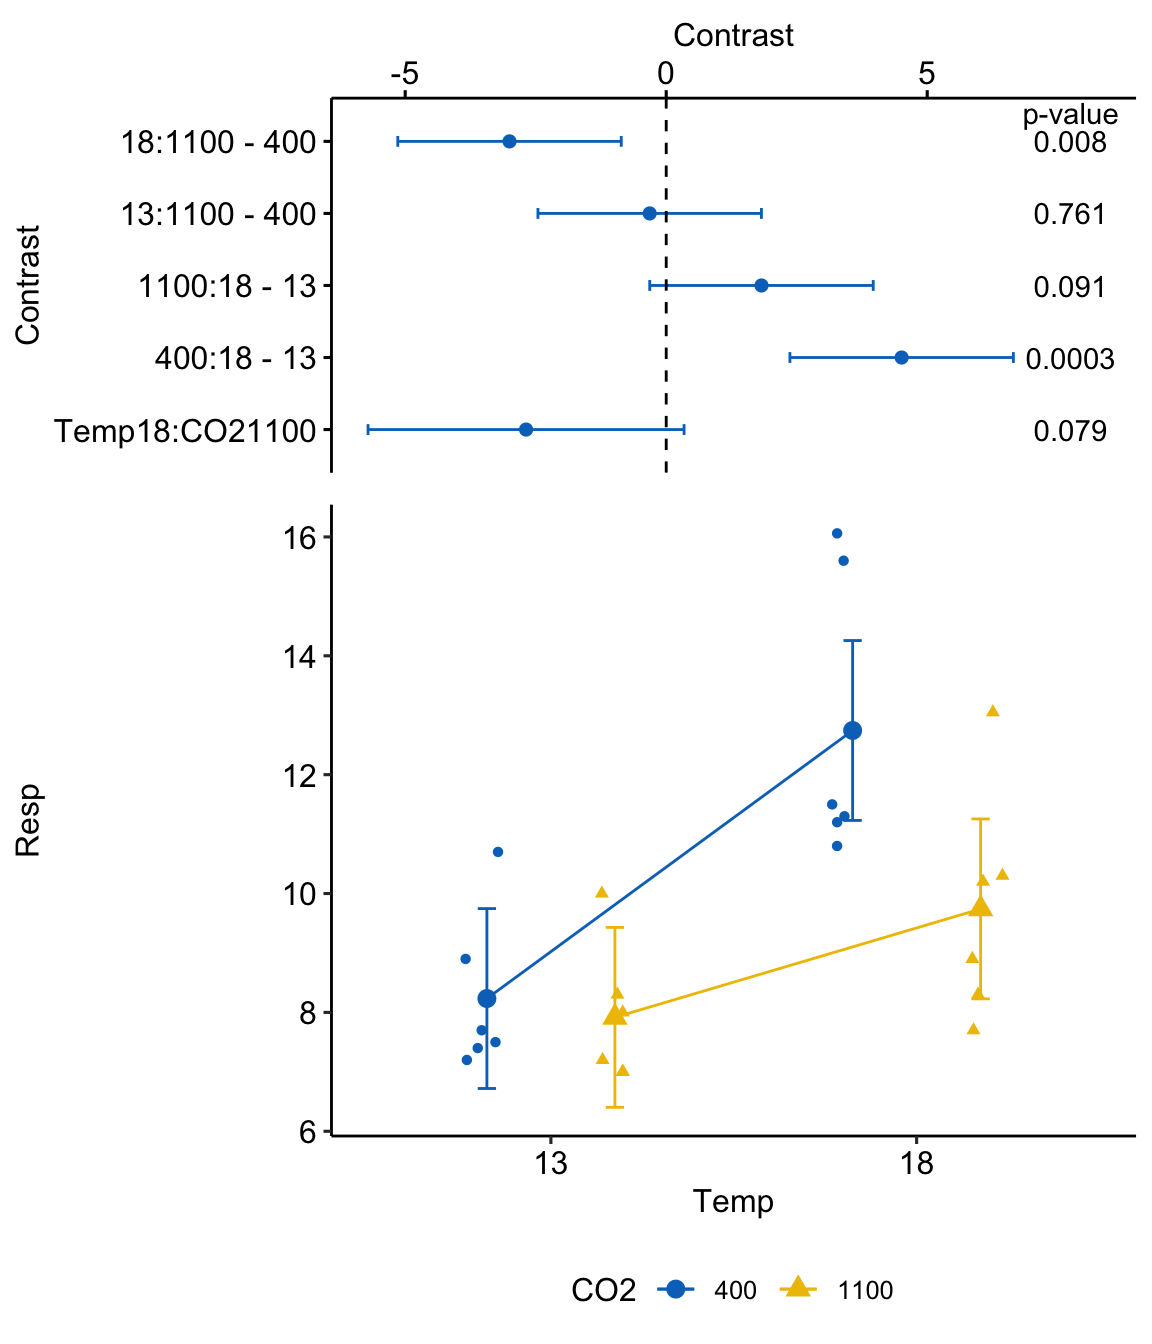
\includegraphics{Walker-elementary-statistical-modeling-draft_files/figure-latex/unnamed-chunk-86-1.pdf}

\hypertarget{plotting-two-factors}{%
\subsection{Plotting two factors}\label{plotting-two-factors}}

The data are from figure 6d. This solution requires computing either the raw or modeled means and errors and adding these to a base ggpubr plot. Many packages have summary statistics functions for means, standard deviations, and standard errors. This is easily done by simply computing the statistics using data.table functionality.

\begin{Shaded}
\begin{Highlighting}[]
\CommentTok{# compute raw statistics}
\CommentTok{# enclosing the line within parentheses prints the result to the console!}
\NormalTok{(exp6d.raw <-}\StringTok{ }\NormalTok{exp6d[}\OperatorTok{!}\KeywordTok{is.na}\NormalTok{(count), .(}\DataTypeTok{count=}\KeywordTok{mean}\NormalTok{(count),}
                       \DataTypeTok{se=}\KeywordTok{sd}\NormalTok{(count)}\OperatorTok{/}\KeywordTok{sqrt}\NormalTok{(.N)),}
                   \DataTypeTok{by=}\NormalTok{.(treatment, strain)]}
\NormalTok{)}
\end{Highlighting}
\end{Shaded}

\begin{verbatim}
##     treatment strain    count       se
## 1:    control     wt 13.08333 2.310904
## 2:    control  sox10 45.61538 6.259903
## 3: transplant     wt 16.35714 2.259552
## 4: transplant  sox10 18.33333 4.536274
\end{verbatim}

Modeled means, standard errors, and confidence limits are conveniently computed using the \texttt{emmeans} (``estimated marginal means'') function from the emmeans package.

\begin{Shaded}
\begin{Highlighting}[]
\CommentTok{# modeled statsistics}
\NormalTok{m1 <-}\StringTok{ }\KeywordTok{glm.nb}\NormalTok{(count }\OperatorTok{~}\StringTok{ }\NormalTok{treatment}\OperatorTok{*}\NormalTok{strain, }\DataTypeTok{data=}\NormalTok{exp6d)}
\NormalTok{(m1.emm <-}\StringTok{ }\KeywordTok{data.table}\NormalTok{(}\KeywordTok{summary}\NormalTok{(}\KeywordTok{emmeans}\NormalTok{(m1, }\DataTypeTok{specs=}\KeywordTok{c}\NormalTok{(}\StringTok{"treatment"}\NormalTok{, }\StringTok{"strain"}\NormalTok{), }\DataTypeTok{type=}\StringTok{"response"}\NormalTok{))))}
\end{Highlighting}
\end{Shaded}

\begin{verbatim}
##     treatment strain response       SE  df asymp.LCL asymp.UCL
## 1:    control     wt 13.08333 2.032161 Inf  9.649528  17.73907
## 2: transplant     wt 16.35714 2.289208 Inf 12.433129  21.51961
## 3:    control  sox10 45.61538 6.132974 Inf 35.048350  59.36837
## 4: transplant  sox10 18.33333 3.871911 Inf 12.119140  27.73391
\end{verbatim}

\begin{Shaded}
\begin{Highlighting}[]
\CommentTok{# change column "response" to "count" for the ggplot}
\KeywordTok{setnames}\NormalTok{(m1.emm, }\DataTypeTok{old=}\StringTok{"response"}\NormalTok{, }\DataTypeTok{new=}\StringTok{"count"}\NormalTok{)}
\end{Highlighting}
\end{Shaded}

\begin{Shaded}
\begin{Highlighting}[]
\CommentTok{#pairs_i <- list(c("sox10", "iap_mo"), c("sox10", "gf"), c("sox10", "wt"))}
\NormalTok{pd =}\StringTok{ }\KeywordTok{position_dodge}\NormalTok{(}\FloatTok{0.7}\NormalTok{)}
\KeywordTok{ggbarplot}\NormalTok{(}\DataTypeTok{x=}\StringTok{"treatment"}\NormalTok{, }
          \DataTypeTok{y=}\StringTok{"count"}\NormalTok{,}
          \DataTypeTok{data=}\NormalTok{exp6d,}
          \DataTypeTok{add=}\KeywordTok{c}\NormalTok{(}\StringTok{"mean"}\NormalTok{),}
          \DataTypeTok{color =} \StringTok{"black"}\NormalTok{,}
          \DataTypeTok{fill =} \StringTok{"strain"}\NormalTok{,}
          \DataTypeTok{palette =} \StringTok{"jco"}\NormalTok{,}
          \DataTypeTok{position =}\NormalTok{ pd,}
          \DataTypeTok{size=}\FloatTok{0.5}\NormalTok{) }\OperatorTok{+}
\StringTok{  }\CommentTok{#stat_compare_means(method = "t.test", comparisons=pairs_i) +}
\StringTok{  }\KeywordTok{ylab}\NormalTok{(}\StringTok{"Neutrophil count"}\NormalTok{) }\OperatorTok{+}
\StringTok{  }\CommentTok{# geom_dotplot(aes(fill=strain),}
\StringTok{  }\CommentTok{#              binaxis='y', stackdir='center', position=pd, show.legend=FALSE,}
\StringTok{  }\CommentTok{#              color="grey") +}
\StringTok{  }\KeywordTok{geom_point}\NormalTok{(}\KeywordTok{aes}\NormalTok{(}\DataTypeTok{fill=}\NormalTok{strain), }\DataTypeTok{position=}\KeywordTok{position_jitterdodge}\NormalTok{(}\DataTypeTok{jitter.width=}\FloatTok{0.2}\NormalTok{), }\DataTypeTok{show.legend=}\OtherTok{FALSE}\NormalTok{, }\DataTypeTok{alpha=}\FloatTok{0.5}\NormalTok{) }\OperatorTok{+}
\StringTok{  }\KeywordTok{geom_errorbar}\NormalTok{(}\DataTypeTok{data=}\NormalTok{m1.emm, }\KeywordTok{aes}\NormalTok{(}\DataTypeTok{x=}\NormalTok{treatment, }\DataTypeTok{ymin=}\NormalTok{asymp.LCL, }\DataTypeTok{ymax=}\NormalTok{asymp.UCL, }\DataTypeTok{group=}\NormalTok{strain),}
                \DataTypeTok{position=}\NormalTok{pd, }\DataTypeTok{width=}\FloatTok{0.1}\NormalTok{) }\OperatorTok{+}
\StringTok{  }\OtherTok{NULL}
\end{Highlighting}
\end{Shaded}

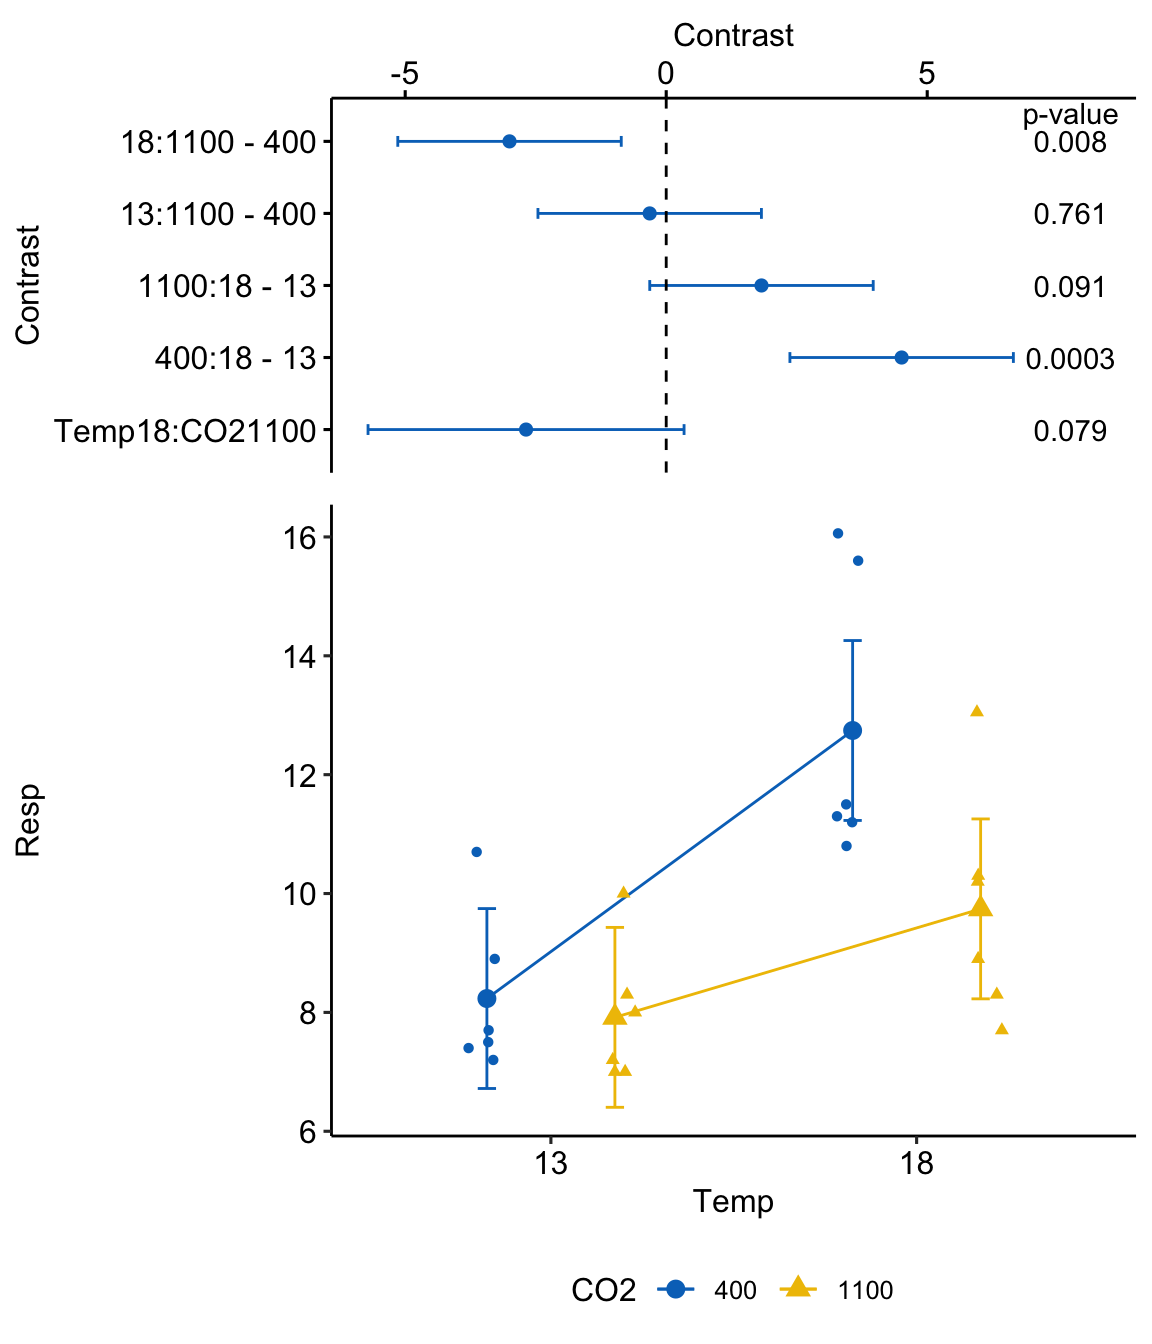
\includegraphics{Walker-elementary-statistical-modeling-draft_files/figure-latex/unnamed-chunk-89-1.pdf}

\hypertarget{interaction-plot}{%
\subsection{Interaction plot}\label{interaction-plot}}

\begin{Shaded}
\begin{Highlighting}[]
\CommentTok{#pairs_i <- list(c("sox10", "iap_mo"), c("sox10", "gf"), c("sox10", "wt"))}

\NormalTok{pd =}\StringTok{ }\KeywordTok{position_dodge}\NormalTok{(}\FloatTok{0.2}\NormalTok{)}
\KeywordTok{ggplot}\NormalTok{(}\DataTypeTok{data=}\NormalTok{m1.emm, }\KeywordTok{aes}\NormalTok{(}\DataTypeTok{x=}\NormalTok{treatment, }\DataTypeTok{y=}\NormalTok{count, }\DataTypeTok{shape=}\NormalTok{strain, }\DataTypeTok{color=}\NormalTok{strain, }\DataTypeTok{group=}\NormalTok{strain)) }\OperatorTok{+}
\StringTok{  }\KeywordTok{geom_point}\NormalTok{(}\DataTypeTok{position=}\NormalTok{pd, }\DataTypeTok{size=}\DecValTok{3}\NormalTok{) }\OperatorTok{+}
\StringTok{  }\KeywordTok{geom_errorbar}\NormalTok{(}\DataTypeTok{data=}\NormalTok{m1.emm, }\KeywordTok{aes}\NormalTok{(}\DataTypeTok{x=}\NormalTok{treatment, }\DataTypeTok{ymin=}\NormalTok{asymp.LCL, }\DataTypeTok{ymax=}\NormalTok{asymp.UCL, }\DataTypeTok{group=}\NormalTok{strain),}\DataTypeTok{position=}\NormalTok{pd, }\DataTypeTok{width=}\FloatTok{0.1}\NormalTok{) }\OperatorTok{+}
\StringTok{  }\KeywordTok{geom_line}\NormalTok{(}\DataTypeTok{position=}\NormalTok{pd) }\OperatorTok{+}
\StringTok{  }\KeywordTok{ylab}\NormalTok{(}\StringTok{"Neutrophil count"}\NormalTok{) }\OperatorTok{+}
\StringTok{  }\KeywordTok{scale_color_jco}\NormalTok{() }\OperatorTok{+}
\StringTok{  }\KeywordTok{theme_pubr}\NormalTok{() }\OperatorTok{+}
\StringTok{  }\OtherTok{NULL}
\end{Highlighting}
\end{Shaded}

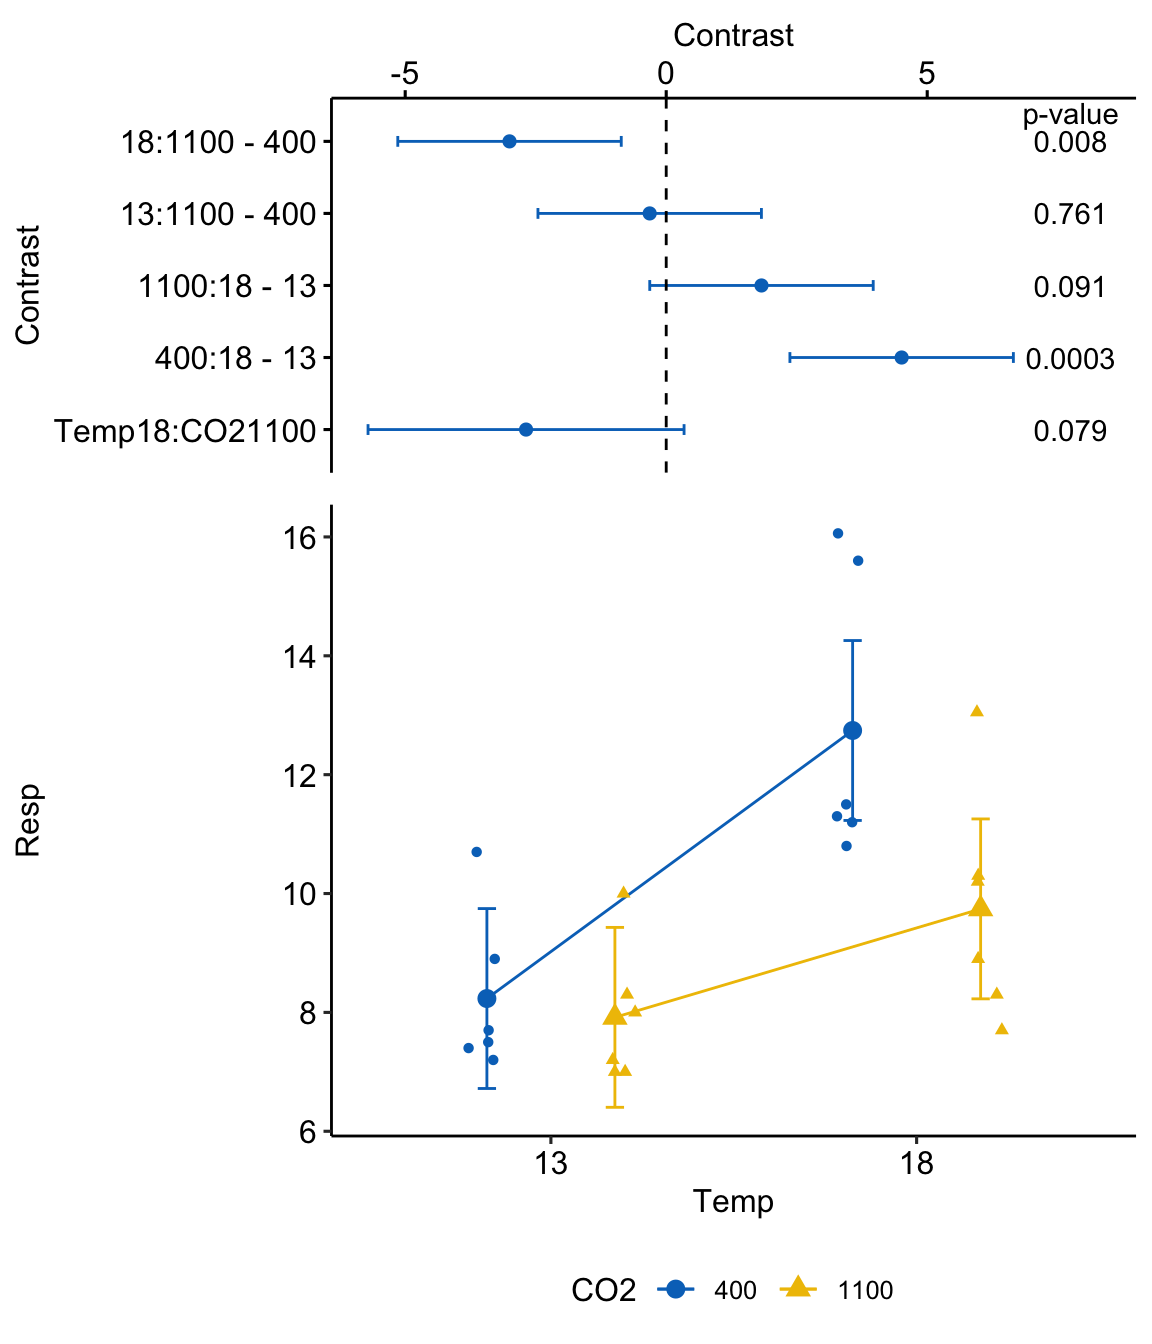
\includegraphics{Walker-elementary-statistical-modeling-draft_files/figure-latex/unnamed-chunk-90-1.pdf}

\hypertarget{plot-components}{%
\subsection{Plot components}\label{plot-components}}

\hypertarget{showing-the-data}{%
\subsubsection{Showing the data}\label{showing-the-data}}

If there are only a few cases per group, there is little reason to summarize the distribution. Instead plot the individual points using a stripchart or a jitter plot

\begin{Shaded}
\begin{Highlighting}[]
\CommentTok{# sample 4 points from each group to make it a small n experiment}
\NormalTok{inc <-}\StringTok{ }\NormalTok{exp2d[, .(}\DataTypeTok{inc=}\KeywordTok{sample}\NormalTok{(}\KeywordTok{min}\NormalTok{(.I)}\OperatorTok{:}\KeywordTok{max}\NormalTok{(.I), }\DecValTok{4}\NormalTok{)), by=donor][, inc]}
\KeywordTok{ggstripchart}\NormalTok{(}\DataTypeTok{x =} \StringTok{"donor"}\NormalTok{,}
             \DataTypeTok{y =} \StringTok{"count"}\NormalTok{,}
             \DataTypeTok{alpha =} \FloatTok{0.5}\NormalTok{,}
             \DataTypeTok{add =} \StringTok{"mean"}\NormalTok{,}
             \DataTypeTok{data =}\NormalTok{ exp2d[inc,])}
\end{Highlighting}
\end{Shaded}

\begin{verbatim}
## Warning: `fun.y` is deprecated. Use `fun` instead.
\end{verbatim}

\begin{verbatim}
## Warning: `fun.ymin` is deprecated. Use `fun.min` instead.
\end{verbatim}

\begin{verbatim}
## Warning: `fun.ymax` is deprecated. Use `fun.max` instead.
\end{verbatim}

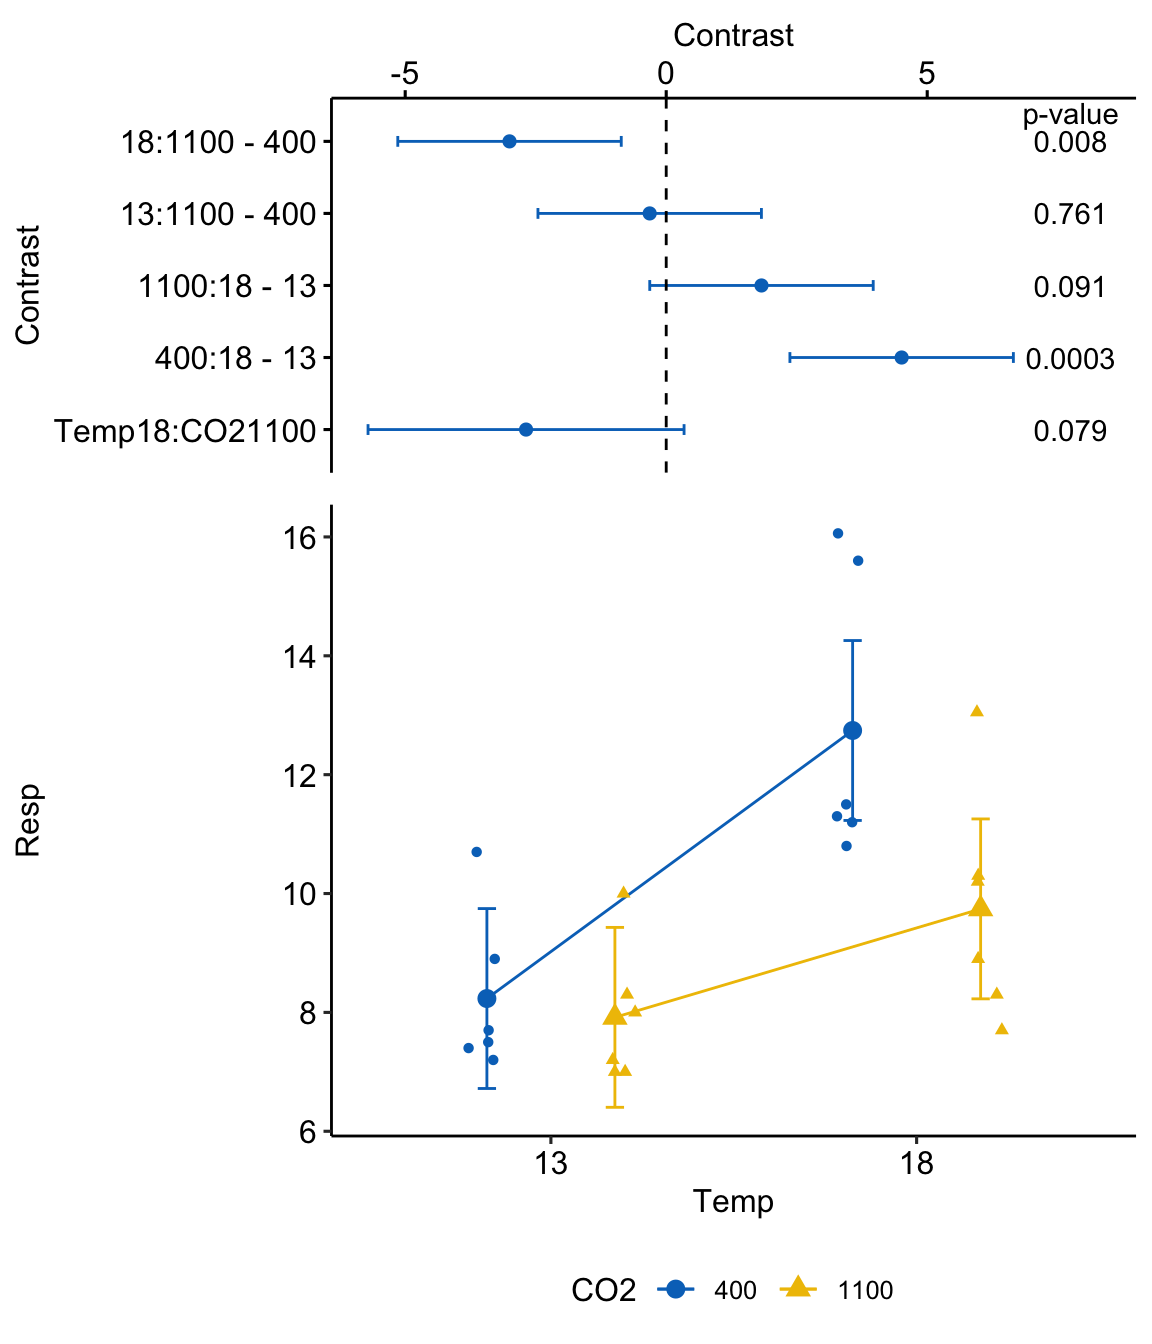
\includegraphics{Walker-elementary-statistical-modeling-draft_files/figure-latex/unnamed-chunk-91-1.pdf}

With more points, a stripchart can be okay but with too many points the distribution might be obscured. Reasonable alternatives are a box plot, a violin plot, and a dotplot.

\begin{Shaded}
\begin{Highlighting}[]
\NormalTok{gg1 <-}\StringTok{ }\KeywordTok{ggstripchart}\NormalTok{(}\DataTypeTok{x =} \StringTok{"donor"}\NormalTok{,}
          \DataTypeTok{y =} \StringTok{"count"}\NormalTok{,}
          \DataTypeTok{fill=}\StringTok{"steelblue"}\NormalTok{,}
          \DataTypeTok{data =}\NormalTok{ exp2d)}

\NormalTok{gg2 <-}\StringTok{ }\KeywordTok{ggboxplot}\NormalTok{(}\DataTypeTok{x =} \StringTok{"donor"}\NormalTok{,}
          \DataTypeTok{y =} \StringTok{"count"}\NormalTok{,}
          \DataTypeTok{fill=}\StringTok{"steelblue"}\NormalTok{,}
          \DataTypeTok{data =}\NormalTok{ exp2d)}

\NormalTok{gg3 <-}\StringTok{ }\KeywordTok{ggviolin}\NormalTok{(}\DataTypeTok{x =} \StringTok{"donor"}\NormalTok{,}
          \DataTypeTok{y =} \StringTok{"count"}\NormalTok{,}
          \DataTypeTok{fill=}\StringTok{"steelblue"}\NormalTok{,}
          \DataTypeTok{data =}\NormalTok{ exp2d)}
\NormalTok{gg4 <-}\StringTok{ }\KeywordTok{ggdotplot}\NormalTok{(}\DataTypeTok{x =} \StringTok{"donor"}\NormalTok{,}
          \DataTypeTok{y =} \StringTok{"count"}\NormalTok{,}
          \DataTypeTok{fill=}\StringTok{"steelblue"}\NormalTok{,}
          \DataTypeTok{data =}\NormalTok{ exp2d)}
\KeywordTok{plot_grid}\NormalTok{(gg1, gg2, gg3, gg4, }\DataTypeTok{nrow=}\DecValTok{2}\NormalTok{)}
\end{Highlighting}
\end{Shaded}

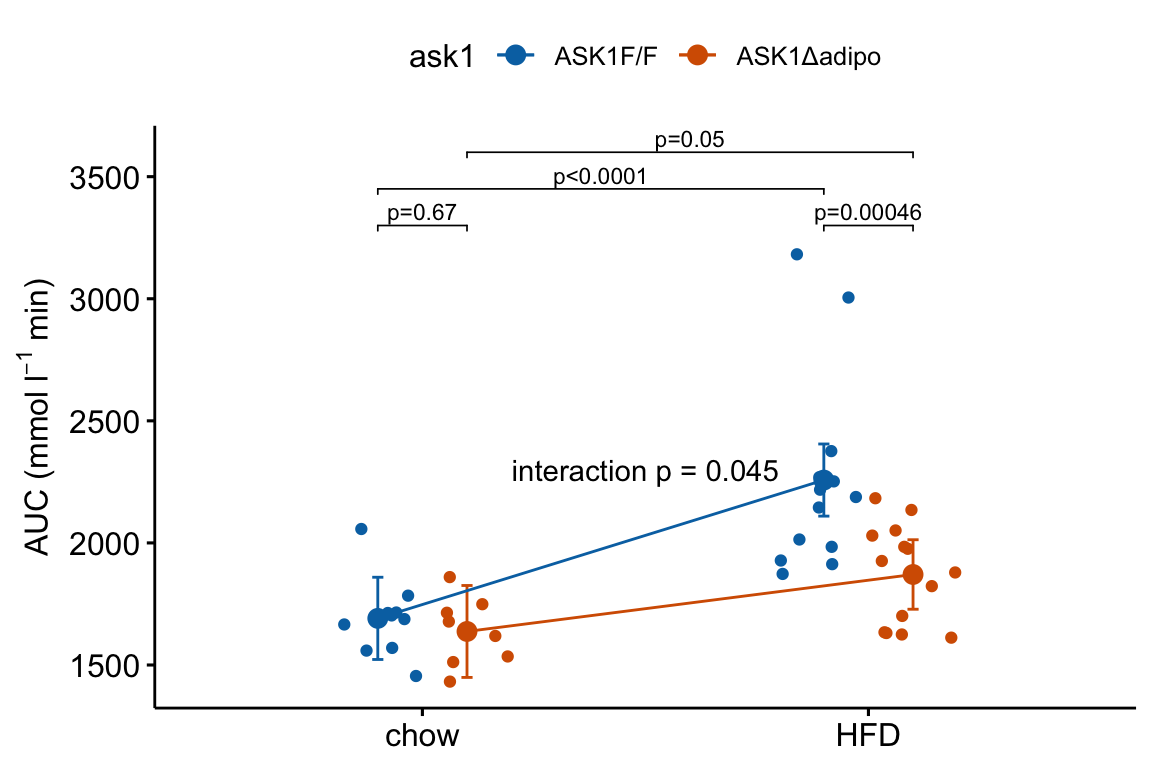
\includegraphics{Walker-elementary-statistical-modeling-draft_files/figure-latex/unnamed-chunk-92-1.pdf}

\hypertarget{part-ii-some-fundamentals-of-statistical-modeling}{%
\chapter*{Part II: Some Fundamentals of Statistical Modeling}\label{part-ii-some-fundamentals-of-statistical-modeling}}
\addcontentsline{toc}{chapter}{Part II: Some Fundamentals of Statistical Modeling}

\hypertarget{variability-and-uncertainty-standard-deviations-standard-errors-confidence-intervals}{%
\chapter{Variability and Uncertainty (Standard Deviations, Standard Errors, Confidence Intervals)}\label{variability-and-uncertainty-standard-deviations-standard-errors-confidence-intervals}}

\textbf{Uncertainty} is the stuff of science. A major goal of statistics is measuring uncertainty. What do we mean by uncertainty? Uncertainty is the error in estimating a parameter, such as the mean of a sample, or the difference in means between two experimental treatments, or the predicted response given a certain change in conditions. Uncertainty is measured with a \textbf{variance} or its square root, which is a \textbf{standard deviation}. The standard deviation of a statistic is also (and more commonly) called a \textbf{standard error}.

Uncertainty emerges because of variability. In any introductory statistics class, students are introduced to two measures of variability, the ``standard deviation'' and the ``standard error.'' These terms are absolutely fundamental to statistics -- they are the start of everything else. Yet, many biology researchers confuse these terms and certainly, introductory students do too.

When a research biologist uses the term ``standard deviation,'' they are probably referring to the sample standard deviation which is a measure of the variability of a sample. When a research biologist uses the term ``standard error,'' they are probably referring to the standard error of a mean, but it could be the standard error of another statistics, such as a difference between means or a regression slope. An important point to remember and understand is that all standard errors \emph{are} standard deviations. This will make more sense soon.

\hypertarget{the-sample-standard-deviation-vs.-the-standard-error-of-the-mean}{%
\section{The sample standard deviation vs.~the standard error of the mean}\label{the-sample-standard-deviation-vs.-the-standard-error-of-the-mean}}

A standard deviation is the square root of the sampling variance.

\hypertarget{sample-standard-deviation}{%
\subsection{Sample standard deviation}\label{sample-standard-deviation}}

The sample standard deviation is a measure of the variability of a sample. For example, were we to look at a histological section of skeletal muscle we would see that the diameter of the fibers (the muscle cells) is variable. We could use imaging software to measure the diameter of a sample of 100 cells and get a \textbf{distribution} like this

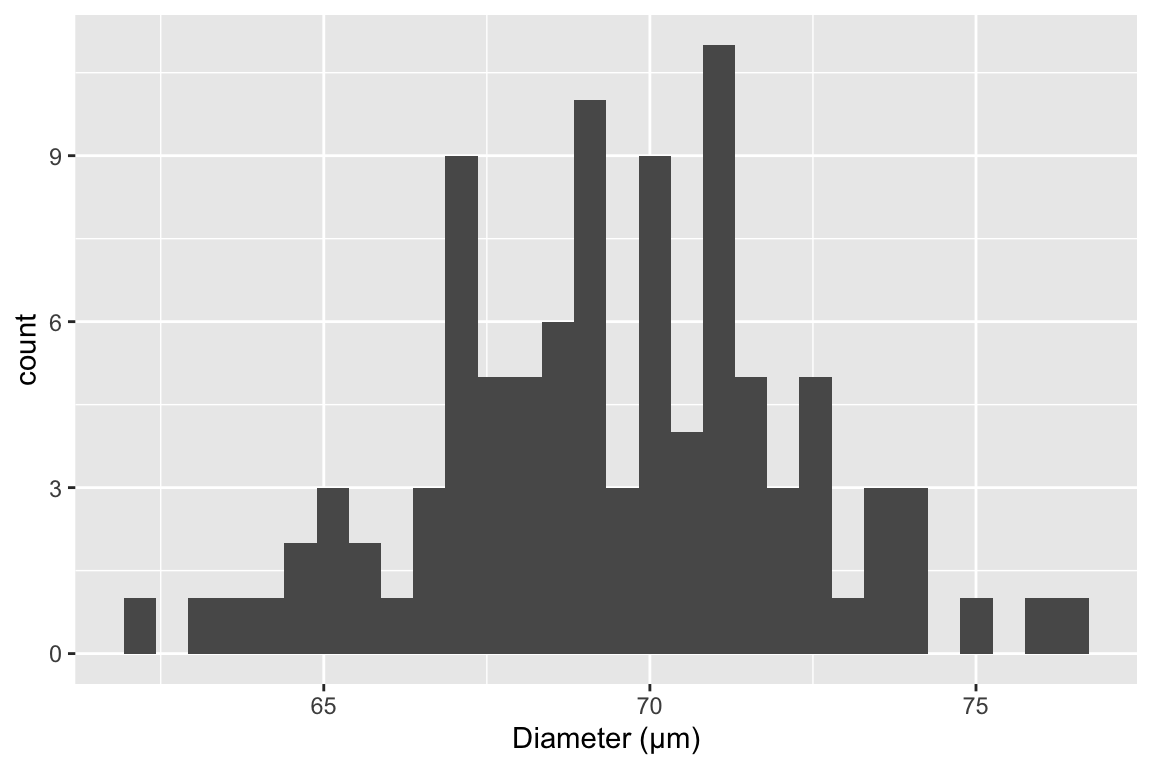
\includegraphics{Walker-elementary-statistical-modeling-draft_files/figure-latex/histogram-1.pdf}

The mean of this sample is 69.4µm and the standard deviation is 2.8 µm. The standard deviation is the square root of the variance, and so computed by

\begin{equation}
s_y = \sqrt{\frac{\sum_{i=1}^n{(y_i - \overline{y})^2}}{n-1}}
\label{eq:variance}
\end{equation}

Memorize this equation. To understand the logic of this measure of variability, note that \(y_i - \overline{y}\) is the \textbf{deviation} of the \(i\)th value from the sample mean, so the numerator is the sum of squared deviations. The numerator is a sum over \(n\) items and the denominator is \(n-1\) so the variance is (almost!) an averaged squared deviation. More variable samples will have bigger deviations and, therefore, bigger average squared deviations. Since the standard deviation is the square root of the variance, a standard deviation is the square root of an average squared deviation. This makes it similar in value to the averaged deviation (or average of the absolute values of the deviations since the average deviation is, by definition of a mean, zero).

\hypertarget{notes-on-the-variance-and-standard-deviation}{%
\subsubsection{Notes on the variance and standard deviation}\label{notes-on-the-variance-and-standard-deviation}}

\begin{enumerate}
\def\labelenumi{\arabic{enumi}.}
\tightlist
\item
  Variances are additive but standard deviations are not. This means that the variance of the sum of two independent (uncorrelated) random variables is simply the sum of the variances of each of the variables. This is important for many statistical analyses.
\item
  The units of variance are the square of the original units, which is awkward for interpretation. The units of a standard deviation is the same as that of the original variable, and so is much easier to interpet.
\item
  For variables that are approximately normally distributed, we can map the standard deviation to the quantiles of the distribution. For example, 68\% of the values are within one standard deviation of the mean, 95\% of the values are within two standard deviations, and 99\% of the values are within three standard deviations.
\end{enumerate}

\hypertarget{standard-error-of-the-mean}{%
\subsection{Standard error of the mean}\label{standard-error-of-the-mean}}

A standard error of a statistic is a measure of the precision of the statistic. The standard error of the mean is a measure of the precision of the estimate of the mean. The standard error of a difference in means is a measure of the precision of the estimate of the difference in means. The smaller the standard error, the more precise the estimate. The standard error of the mean (SEM) is computed as

\begin{equation}
SEM = \frac{s_y}{\sqrt{n}}
\label{eq:se}
\end{equation}

The SEM is often denoted \(s_{\bar{y}}\) to indicate that it is a standard deviation of the mean (\(\bar{y}\)).

\hypertarget{the-standard-error-of-the-mean-can-be-thought-of-as-a-standard-deviation-of-an-infinitely-long-column-of-re-sampled-means}{%
\subsubsection{The standard error of the mean can be thought of as a standard deviation of an infinitely long column of re-sampled means}\label{the-standard-error-of-the-mean-can-be-thought-of-as-a-standard-deviation-of-an-infinitely-long-column-of-re-sampled-means}}

In what sense is a standard error a standard deviation? This is kinda weird. If we sample 100 cells in the slide of muscle tissue and compute the mean diameter, how can the mean have a standard deviation? There is only one value!

To understand how the SEM is a standard deviation, imagine that we sample \(n\) values from \(N(\mu, \sigma^2)\) (a normal distribution with mean \(\mu\) and variance \(\sigma^2\). The mean of our sample is an estimate of \(\mu\) the standard deviation of sample is an estimate of \(\sigma\)) an infinite number of times and each time, we write down the mean of the new sample. The standard deviation of this infinitely long column of means is the standard error of the mean. Our observed SEM is an estimate of this true value because our observed standard deviation is an estimate of \(\sigma\).

\hypertarget{a-standard-deviation-can-be-computed-for-any-statistic-these-are-all-standard-errors.}{%
\subsubsection{A standard deviation can be computed for any statistic -- these are all standard errors.}\label{a-standard-deviation-can-be-computed-for-any-statistic-these-are-all-standard-errors.}}

The SEM is only one kind of standard error. A standard deviation can be computed for any statistic -- these are all standard errors. For some statistics, such as the mean, the standard error can be computed directly using an equation, such as that for the SEM (equation \eqref{eq:se}). For other statistics, a computer intensive method known as the \textbf{bootstrap} is necessary to compute a standard error. We will return to the bootstrap in Section \ref{bootstrap}.

\hypertarget{notes-on-standard-errors}{%
\subsubsection{Notes on standard errors}\label{notes-on-standard-errors}}

\begin{enumerate}
\def\labelenumi{\arabic{enumi}.}
\tightlist
\item
  The units of a standard error are the units of the measured variable.
\item
  A standard error is proportional to sample variability (the sample standard deviation, \(s_y\)) and inversely proportional to sample size (\(n\)). Sample variability is a function of both natural variation (there really is variation in diameter among fibers in the quadriceps muscle) and measurement error (imaging software with higher resolution can measure a diameter with less error). Since the SEM is a measure of the precision of estimating a mean, this means this precision will increase (or the SEM will decrease) if 1) an investigator uses methods that reduce measurement error and 2) an investigator computes the mean from a larger sample.
\item
  This last point (the SEM decreases with sample size) seems obvious when looking at equation \eqref{eq:se}, since \(n\) is in the denominator. Of course \(n\) is also in the denominator of equation \eqref{eq:variance} for the sample standard deviation but the standard deviation does not decrease as sample size increases. First this wouldn't make any sense -- variability is variability. A sample of 10,000 cell diameters should be no more variable than a sample of 100 cell diameters (think about if you agree with this or not). Second, this should also be obvious from equation \eqref{eq:variance}. The standard deviation is the square root of an average and averages don't increase with the number of things summed since both the the numerator (a sum) and denominator increase with \(n\).
\end{enumerate}

\hypertarget{using-google-sheets-to-generate-fake-data-to-explore-the-standard-error}{%
\section{Using Google Sheets to generate fake data to explore the standard error}\label{using-google-sheets-to-generate-fake-data-to-explore-the-standard-error}}

In statistics we are interested in estimated parameters of a \textbf{population} using measures from a \textbf{sample}. The goal in this section is to use Google Sheets (or Microsoft Excel) to use fake data to discover the behavior of sampling and to gain some intuition about uncertainty using standard errors.

\hypertarget{steps}{%
\subsection{Steps}\label{steps}}

\begin{enumerate}
\def\labelenumi{\arabic{enumi}.}
\tightlist
\item
  Open Google Sheets
\item
  In cell A1 type ``mu''. mu is the greek letter \(\mu\) and is very common notation for the poplation value (the TRUE value!) of the mean of some hypothetical measure. In cell B1, insert some number as the value of \(\mu\). Any number! It can be negative or positive.
\item
  In cell A2 type ``sigma''. sigma is the greek letter \(\sigma\). \(\sigma^2\) is very common (universal!) notation for the population (TRUE) variance of some measure or parameter. Notice that the true (population) values of the mean and variance are greek letters. This is pretty standard in statistics. In cell B2, insert some positive number (standard deviations are the positive square roots of the variance).
\item
  In cell A8 type the number 1
\item
  In cell A9 insert the equation ``=A8 + 1''. What is this equation doing? It is adding the number 1 to to the value in the cell above, so the resulting value should be 2.
\item
  In Cell B8, insert the equation "=normsinv(rand())*\$B\$2 + \$B\$1". The first part of the equation creates a random normal variable with mean 0 and standard deviation 1. multiplication and addition transform this to a random normal variable with mean \(\mu\) and standard deviation \(\sigma\) (the values you set in cells B1 and B2).
\item
  copy cell B8 and paste into cell B9. Now Higlight cells A9:B9 and copy the equations down to row 107. You now have 100 random variables sampled from a infinite population with mean \(\mu\) and standard deviation \(\sigma\).
\item
  In cell A4 write ``mean 10''. In cell B4 insert the equation ``=average(B8:B17)''. The resulting value is the \textbf{sample mean} of the first 10 random variables you created. Is the mean close to \(\mu\)?
\item
  In cell A5 write ``sd 10''. In cell B5 insert the equation ``stdev(B8:B17)''. The result is the \textbf{sample standard deviation} of the first 10 random variables. Is this close to \(\sigma\)?
\item
  In cell A6 write ``mean 100''. In cell B6 insert the equation ``=average(B8:B107)''. The resulting value is the \textbf{sample mean} of the all 100 random variables you created. Is this mean closer to \(\mu\) than mean 10?
\item
  In cell A7 write ``sd 100''. In cell B7 insert the equation ``=stdev(B8:B107)''. The resulting value is the \textbf{sample standard deviation} of the all 100 random variables you created. Is this SD closer to \(\sigma\) than sd 10?
\end{enumerate}

The sample standard deviation is a measure of the variability of the sample. The more spread out the sample (the further each value is from the mean), the bigger the sample standard deviation. The sample standard deviation is most often simply known as ``The'' standard deviation, which is a bit misleading since there are many kinds of standard deviations!

Remember that your computed mean and standard deviations are estimates computed from a sample. They are estimates of the true values \(\mu\) and \(\sigma\). Explore the behavior of the sample mean and standard deviation by re-calculating the spreadsheet. In Excel, a spreadsheet is re-calculated by simultaneously pressing the command and equal key. In Google, command-R recalculates but is painfully slow. Instead, if using Google Sheets, just type the number 1 into a blank cell, and the sheet recalculates quickly. Do it again. And again.

Each time you re-calculate, a new set of random numbers are generated and the new means and standard deviations are computed. Compare mean 10 and mean 100 each re-calculation. Notice that these estimates are variable. They change with each re-calculation. How variable is mean 10 compared to mean 100? The variability of the estimate of the mean is a measure of \textbf{uncertainty} in the estimate. Are we more uncertain with mean 10 or with mean 100? This variability is measured by a standard deviation. This \textbf{standard deviation of the mean} is also called the \textbf{standard error of the mean}. Many researchers are loose with terms and use ``The'' standard error to mean the standard error of the mean, even though there are many kinds of standard errors. In general, ``standard error''" is abbreviated as ``SE.'' Sometimes ``standard error of the mean'' is specifically abbreviated to ``SEM.''

The standard error of the mean is a measure of the precision in estimating the mean. The smaller the value the more precise the estimate. The standard error of the mean \emph{is} a standard deviation of the mean. This is kinda weird. If we sample a population one time and compute a mean, how can the mean have a standard deviation? There is only one value! And we compute this value using the sample standard deviation: \(SEM = \frac{SD}{\sqrt{N}}\). To understand how the SEM is a standard deviation, Imagine recalculating the spread sheet an infinite number of times and each time, you write down the newly computed mean. The standard error of the mean is the standard deviation of this infinitely long column of means.

\hypertarget{using-r-to-generate-fake-data-to-explore-the-standard-error}{%
\section{Using R to generate fake data to explore the standard error}\label{using-r-to-generate-fake-data-to-explore-the-standard-error}}

note that I use ``standard deviation'' to refer to the sample standard deviation and ``standard error'' to refer to the standard error of the mean (again, we can compute standard errors as a standard deviation of any kind of estimate)

\hypertarget{part-i}{%
\subsection{part I}\label{part-i}}

In the exercise above, you used Google Sheets to generate \(p\) columns of fake data. Each column had \(n\) elements, so the matrix of fake data was \(n \times m\) (it is standard in most fields to specify a matrix as rows by columns). This is \emph{much} easier to do in R and how much grows exponentially as the size of the matrix grows.

To start, we just generate a \(n \times p\) matrix of normal random numbers.

\begin{Shaded}
\begin{Highlighting}[]
\CommentTok{# R script to gain some intuition about standard deviation (sd) and standard error (se)}
\CommentTok{# you will probably need to install ggplot2 using library(ggplot2) }
\NormalTok{n <-}\StringTok{ }\DecValTok{6} \CommentTok{# sample size}
\NormalTok{p <-}\StringTok{ }\DecValTok{100} \CommentTok{# number of columns of fake data to generate}
\NormalTok{fake_data <-}\StringTok{ }\KeywordTok{matrix}\NormalTok{(}\KeywordTok{rnorm}\NormalTok{(n}\OperatorTok{*}\NormalTok{p, }\DataTypeTok{mean=}\DecValTok{0}\NormalTok{, }\DataTypeTok{sd=}\DecValTok{1}\NormalTok{), }\DataTypeTok{nrow=}\NormalTok{n, }\DataTypeTok{ncol=}\NormalTok{p) }\CommentTok{# create a matrix}
\end{Highlighting}
\end{Shaded}

the 3rd line is the cool thing about R. In one line I'm creating a dataset with \(n\) rows and \(p\) columns. Each column is a sample of the standard normal distribution which by definition has mean zero and standard deviation of 1. But, and this is important, any sample from this distribution will not have exactly mean zero and standard deviation of 1, because it's a sample, the mean and standard deviation will have some small errror from the truth. The line has two parts to it: first I'm using the function ``rnorm'' (for random normal) to create a vector of n*m random, normal deviates (draws from the random normal distribution) and then I'm organizing these into a matrix (using the function ``matrix'')

To compute the vector of means, standard deviations, and standard errors for each column of \texttt{fake\_data}, use the \texttt{apply()} function.

\begin{Shaded}
\begin{Highlighting}[]
\NormalTok{means <-}\StringTok{ }\KeywordTok{apply}\NormalTok{(fake_data,}\DecValTok{2}\NormalTok{,mean) }\CommentTok{# the apply function is super useful}
\NormalTok{sds <-}\StringTok{ }\KeywordTok{apply}\NormalTok{(fake_data,}\DecValTok{2}\NormalTok{,sd)}
\NormalTok{sems <-}\StringTok{ }\NormalTok{sds}\OperatorTok{/}\KeywordTok{sqrt}\NormalTok{(n)}
\end{Highlighting}
\end{Shaded}

\texttt{apply()} is a workhorse in many R scripts and is often used in R scripts in place of a for-loop (see below) because it takes fewer lines of code.

The SEM is the standard deviation of the mean, so let's see if the standard deviation of the means is close to the true standard error. We sampled from a normal distribution with SD=1 so the true standard is

\begin{Shaded}
\begin{Highlighting}[]
\DecValTok{1}\OperatorTok{/}\KeywordTok{sqrt}\NormalTok{(n)}
\end{Highlighting}
\end{Shaded}

\begin{verbatim}
## [1] 0.4082483
\end{verbatim}

and the standard deviation of the \(p\) means is

\begin{Shaded}
\begin{Highlighting}[]
\KeywordTok{sd}\NormalTok{(means)}
\end{Highlighting}
\end{Shaded}

\begin{verbatim}
## [1] 0.3731974
\end{verbatim}

Questions

\begin{enumerate}
\def\labelenumi{\arabic{enumi}.}
\tightlist
\item
  how close is \texttt{sd(means)} to the true SE?
\item
  change p above to 1000. Now how close is sd(means) to the true SE?
\item
  change p above to 10,000. Now how close is sd(means) to the true SE?
\end{enumerate}

\hypertarget{part-ii---means}{%
\subsection{part II - means}\label{part-ii---means}}

This is a visualization of the spread, or variability, of the sampled means

\begin{Shaded}
\begin{Highlighting}[]
\KeywordTok{qplot}\NormalTok{(means)}
\end{Highlighting}
\end{Shaded}

\begin{verbatim}
## `stat_bin()` using `bins = 30`. Pick better value with `binwidth`.
\end{verbatim}

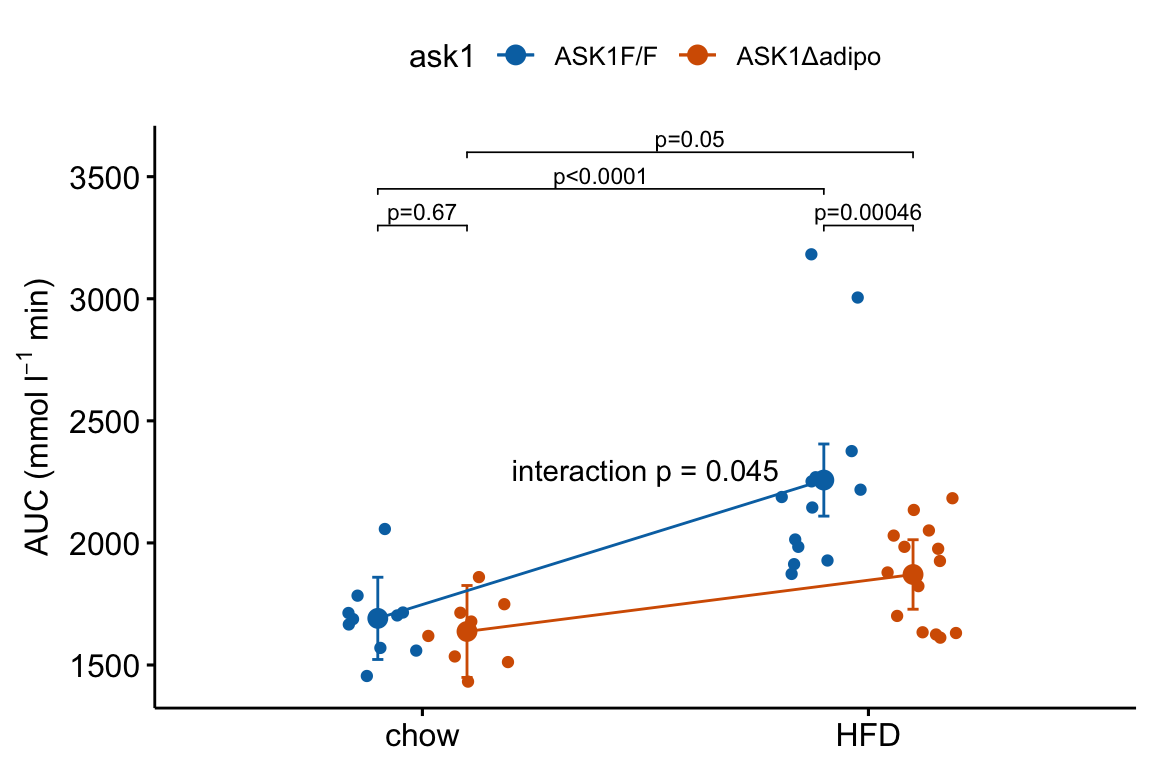
\includegraphics{Walker-elementary-statistical-modeling-draft_files/figure-latex/unnamed-chunk-96-1.pdf}

Compute the mean of the means

\begin{Shaded}
\begin{Highlighting}[]
\KeywordTok{mean}\NormalTok{(means)}
\end{Highlighting}
\end{Shaded}

\begin{verbatim}
## [1] -0.039961
\end{verbatim}

Questions

\begin{enumerate}
\def\labelenumi{\arabic{enumi}.}
\tightlist
\item
  Remember that the true mean is zero. How close, in general, are the sampled means to the true mean. How variable are the means? How is this quantified?
\item
  change n to 100, then replot. Are the means, in general, closer to the true mean? How variable are the means now?
\item
  Is the mean estimated with \(n=100\) closer to the truth, in general, then the mean estimated with \(n=6\)?
\item
  Redo with \(n=10000\)
\end{enumerate}

\hypertarget{part-iii---how-do-sd-and-se-change-as-sample-size-n-increases}{%
\subsection{part III - how do SD and SE change as sample size (n) increases?}\label{part-iii---how-do-sd-and-se-change-as-sample-size-n-increases}}

\begin{Shaded}
\begin{Highlighting}[]
\KeywordTok{mean}\NormalTok{(sds)}
\end{Highlighting}
\end{Shaded}

\begin{verbatim}
## [1] 1.017144
\end{verbatim}

Questions

\begin{enumerate}
\def\labelenumi{\arabic{enumi}.}
\tightlist
\item
  what is the mean of the standard deviations when n=6 (set p=1000)
\item
  what is the mean of the standard deviations when n=100 (set p=1000)
\item
  when n = 1000? (set p=1000)
\item
  when n = 10000? (set p=1000)
\item
  how does the mean of the standard deviations change as n increases (does it get smaller? or stay about the same size)
\item
  repeat the above with SEM
\end{enumerate}

\begin{Shaded}
\begin{Highlighting}[]
\KeywordTok{mean}\NormalTok{(sems)}
\end{Highlighting}
\end{Shaded}

\begin{verbatim}
## [1] 0.4152472
\end{verbatim}

Congratulations, you have just done a Monte Carlo simulation!

\hypertarget{part-iv-generating-fake-data-with-for-loops}{%
\subsection{Part IV -- Generating fake data with for-loops}\label{part-iv-generating-fake-data-with-for-loops}}

A \textbf{for-loop} is used to iterate a computation.

\begin{Shaded}
\begin{Highlighting}[]
\NormalTok{n <-}\StringTok{ }\DecValTok{6} \CommentTok{# sample size}
\NormalTok{n_iter <-}\StringTok{ }\DecValTok{10}\OperatorTok{^}\DecValTok{5} \CommentTok{# number of iterations of loop (equivalent to p)}
\NormalTok{means <-}\StringTok{ }\KeywordTok{numeric}\NormalTok{(n_iter)}
\NormalTok{sds <-}\StringTok{ }\KeywordTok{numeric}\NormalTok{(n_iter)}
\NormalTok{sems <-}\StringTok{ }\KeywordTok{numeric}\NormalTok{(n_iter)}
\ControlFlowTok{for}\NormalTok{(i }\ControlFlowTok{in} \DecValTok{1}\OperatorTok{:}\NormalTok{n_iter)\{}
\NormalTok{  y <-}\StringTok{ }\KeywordTok{rnorm}\NormalTok{(n) }\CommentTok{# mean=0 and sd=1 are default so not necessary to specify}
\NormalTok{  means[i] <-}\StringTok{ }\KeywordTok{mean}\NormalTok{(y)}
\NormalTok{  sds[i] <-}\StringTok{ }\KeywordTok{sd}\NormalTok{(y)}
\NormalTok{  sems[i] <-}\StringTok{ }\KeywordTok{sd}\NormalTok{(y)}\OperatorTok{/}\KeywordTok{sqrt}\NormalTok{(n)}
\NormalTok{\}}
\KeywordTok{sd}\NormalTok{(means)}
\end{Highlighting}
\end{Shaded}

\begin{verbatim}
## [1] 0.4090702
\end{verbatim}

\begin{Shaded}
\begin{Highlighting}[]
\KeywordTok{mean}\NormalTok{(sems)}
\end{Highlighting}
\end{Shaded}

\begin{verbatim}
## [1] 0.3883867
\end{verbatim}

Questions

\begin{enumerate}
\def\labelenumi{\arabic{enumi}.}
\tightlist
\item
  What do \texttt{sd(means)} and \texttt{mean(sems)} converge to as \texttt{n\_iter} is increased from 100 to 1000 to 10,000?
\item
  Do they converge to the same number?
\item
  Should they?
\item
  What is the correct number?
\end{enumerate}

Question number 4 is asking what is E(SEM), the ``expected standard error of the mean''. There is a very easy formula to compute this. What is it?

\hypertarget{bootstrap}{%
\section{Bootstrapped standard errors}\label{bootstrap}}

The bootstrap is certainly one of the most valuable tools invented in modern statistics. But, it's not only a useful tool for applied statistics, it's a useful tool for understanding statistics. Playing with a parametric bootstrap will almost certainly induce an ``aha, so that's what statisticians mean by \ldots{}'' moment.

To understand the bootstrap, let's review a standard error. A \emph{parametric} standard error of a mean is the \emph{expected} standard deviation of an infinite number of means. A standard error of any statistic is the \emph{expected} standard deviation of that statistic. I highlight \emph{expected} to emphasize that parametric standard errors assume a certain distribution (not necessarily a Normal distribution, although the equation for the SEM in Equation \eqref{eq:se} assumes a normal distribution if the standard deviation is computed as in Equation \eqref{eq:sd}).

A bootstrapped standard error of a statistic is the \textbf{empirical} standard deviation of the statistic from a finite number of \emph{samples}. The basic algorithm for a bootstrap is (here ``the statistic'' is the mean of the sample)

\begin{enumerate}
\def\labelenumi{\arabic{enumi}.}
\tightlist
\item
  sample \(n\) values from a probability distribution
\item
  compute the mean
\item
  repeat step 1 and 2 many times
\item
  for a bootstrapped standard error, compute the standard deviation of the set of means saved from each iteration of steps 1 and 2.
\end{enumerate}

The probability distribution can come from two sources:

\begin{enumerate}
\def\labelenumi{\arabic{enumi}.}
\tightlist
\item
  A \textbf{parametric bootstrap} uses samples from a parametric probability distribution, such as a Normal distribution or a poisson distribution (remember, these are ``parametric'' because the distribution is completely described by a set of parameters). A good question is why bother? In general, one would use a parametric bootstrap for a statistic for which there is no formula for the standard error, but the underlying data come from a parametric probability distribution.
\item
  A \textbf{non-parametric} bootstrap uses \emph{resamples from the data}. The data are resampled \emph{with replacement}. ``Resample with replacement'' means to sample \(n\) times from the full set of observed values. If we were to do this manually, we would i) write down each value of the original sample on its own piece of paper and throw all pieces into a hat. ii) pick a paper from the hat, add its value to sample \(i\), and return the paper to the hat. iii) repeat step ii \(n\) times, where \(n\) is the original sample size. The new sample contains some values multiple times (papers that were picked out of the hat more than once) and is missing some values (papers that were not picked out in any of the \(n\) picks). A good question is, why bother? A non-parametric bootstrap assumes no specific \emph{parametric} probability distribution but it does assume the distributio of the observed sample is a good approximation of the true population distribution (in which case, the probability of picking a certain value is a good approximation to the true probability).
\end{enumerate}

\hypertarget{an-example-of-bootstrapped-standard-errors-using-vole-data}{%
\subsection{An example of bootstrapped standard errors using vole data}\label{an-example-of-bootstrapped-standard-errors-using-vole-data}}

Let's use the vole data to explore the bootstrap and ``resampling''. The data are archived at Dryad Repository. Use the script in Section \ref{vole-data} to wrangle the data into a usable format.

\begin{enumerate}
\def\labelenumi{\arabic{enumi}.}
\tightlist
\item
  URL: \url{https://datadryad.org//resource/doi:10.5061/dryad.31cc4}
\item
  file: RSBL-2013-0432 vole data.xlsx
\item
  sheet: COLD VOLES LIFESPAN
\end{enumerate}

The data are the measured lifespans of the short-tailed field vole (\emph{Microtus agrestis}) under three different experimental treatments: vitamin E supplementation, vitamin C supplementation, and control (no vitamin supplementation). Vitamins C and E are antioxidants, which are thought to be protective of basic cell function since they bind to the cell-damaging reactive oxygen species that result from cell metabolism.

Let's compute the standard error of the mean of the control group lifespan using both a parametric and a nonparametric bootstrap. To implement the algorithm above using easy-to-understand code, I'll first extract the set of lifespan values for the control group and assign it to its own variable.

\begin{Shaded}
\begin{Highlighting}[]
\NormalTok{control_voles <-}\StringTok{ }\NormalTok{vole[treatment}\OperatorTok{==}\StringTok{"control"}\NormalTok{, lifespan]}
\end{Highlighting}
\end{Shaded}

\texttt{{[}treatment=="control",\ {]}} indexes the rows (that is, returns the row numbers) that satisfy the condtion \texttt{treatment\ =\ "control"}. Or, put another way, it selects the \textbf{subset} of rows that contain the value ``control'' in the column ``treatment''. \texttt{{[},\ lifespan{]}} indexes the column labeled ``lifespan''. Combined, these two indices extract the values of the column ``lifespan'' in the subset of rows that contain the value ``control'' in the column ``treatment''. The resulting vector of values is assigned to the variable ``control\_voles''.

\hypertarget{parametric-bootstrap}{%
\subsubsection{parametric bootstrap}\label{parametric-bootstrap}}

\begin{Shaded}
\begin{Highlighting}[]
\CommentTok{# we'll use these as parameters for parametric bootstrap}
\NormalTok{n <-}\StringTok{ }\KeywordTok{length}\NormalTok{(control_voles)}
\NormalTok{mu <-}\StringTok{ }\KeywordTok{mean}\NormalTok{(control_voles)}
\NormalTok{sigma <-}\StringTok{ }\KeywordTok{sd}\NormalTok{(control_voles)}

\NormalTok{n_iter <-}\StringTok{ }\DecValTok{1000} \CommentTok{# number of bootstrap iterations, or p}
\NormalTok{means <-}\StringTok{ }\KeywordTok{numeric}\NormalTok{(n_iter) }\CommentTok{# we will save the means each iteration to this}

\ControlFlowTok{for}\NormalTok{(iter }\ControlFlowTok{in} \DecValTok{1}\OperatorTok{:}\NormalTok{n_iter)\{ }\CommentTok{# this line sets up the number of iterations, p}
\NormalTok{  fake_sample <-}\StringTok{ }\KeywordTok{rnorm}\NormalTok{(n, }\DataTypeTok{mean=}\NormalTok{mu, }\DataTypeTok{sd=}\NormalTok{sigma)}
\NormalTok{  means[iter] <-}\StringTok{ }\KeywordTok{mean}\NormalTok{(fake_sample)}
\NormalTok{\}}
\NormalTok{(se_para_boot <-}\StringTok{ }\KeywordTok{sd}\NormalTok{(means))}
\end{Highlighting}
\end{Shaded}

\begin{verbatim}
## [1] 30.49765
\end{verbatim}

\hypertarget{non-parametric-bootstrap}{%
\subsubsection{non-parametric bootstrap}\label{non-parametric-bootstrap}}

\begin{Shaded}
\begin{Highlighting}[]
\NormalTok{n_iter <-}\StringTok{ }\DecValTok{1000} \CommentTok{# number of bootstrap iterations, or p}
\NormalTok{means <-}\StringTok{ }\KeywordTok{numeric}\NormalTok{(n_iter) }\CommentTok{# we will save the means each iteration to this}
\NormalTok{inc <-}\StringTok{ }\DecValTok{1}\OperatorTok{:}\NormalTok{n }\CommentTok{# inc indexes the elements to sample. By setting inc to 1:n prior to the loop, the first mean that is computed is the observed mean}
\ControlFlowTok{for}\NormalTok{(iter }\ControlFlowTok{in} \DecValTok{1}\OperatorTok{:}\NormalTok{n_iter)\{ }\CommentTok{# this line sets up the number of iterations, p}
\NormalTok{  means[iter] <-}\StringTok{ }\KeywordTok{mean}\NormalTok{(control_voles[inc]) }\CommentTok{# inc is the set of rows to include in the computation of the mean.}
\NormalTok{  inc <-}\StringTok{ }\KeywordTok{sample}\NormalTok{(}\DecValTok{1}\OperatorTok{:}\NormalTok{n, }\DataTypeTok{replace=}\OtherTok{TRUE}\NormalTok{) }\CommentTok{# re-sample for the next iteration}
\NormalTok{\}}
\NormalTok{(se_np_boot <-}\StringTok{ }\KeywordTok{sd}\NormalTok{(means))}
\end{Highlighting}
\end{Shaded}

\begin{verbatim}
## [1] 32.47356
\end{verbatim}

The parametric bootstrapped SEM is 30.5. The non-parametric bootstrapped SEM is 32.47. Run these several times to get a sense how much variation there is in the bootstrapped estimate of the SEM given the number of iterations. Compute the \textbf{parametric} standard error using equation \eqref{eq:se} and compare to the bootstrapped values.

\hypertarget{confidence-interval}{%
\section{Confidence Interval}\label{confidence-interval}}

Here I introduce a \textbf{confidence interval} of a sample mean but the concept is easily generalized to any parameter. The mean of the Control voles is 503.4 and the SE of the mean is 31.61. The SE is used to construct the lower and upper boundary of a ``1 - \(\alpha\)'' confidence interval using \texttt{lower\ \textless{}-\ mean(x)\ +\ qt(alpha/2,\ df\ =\ n-1)*se(x)} and \texttt{upper\ \textless{}-\ mean(x)\ +\ qt(1-(alpha/2),\ df\ =\ n-1)*se(x)}.

\begin{Shaded}
\begin{Highlighting}[]
\NormalTok{(lower <-}\StringTok{ }\KeywordTok{mean}\NormalTok{(control_voles) }\OperatorTok{+}\StringTok{ }\KeywordTok{qt}\NormalTok{(}\FloatTok{0.05}\OperatorTok{/}\DecValTok{2}\NormalTok{, }\DataTypeTok{df=}\NormalTok{(n}\DecValTok{-1}\NormalTok{))}\OperatorTok{*}\KeywordTok{sd}\NormalTok{(control_voles)}\OperatorTok{/}\KeywordTok{sqrt}\NormalTok{(n))}
\end{Highlighting}
\end{Shaded}

\begin{verbatim}
## [1] 440.0464
\end{verbatim}

\begin{Shaded}
\begin{Highlighting}[]
\NormalTok{(upper <-}\StringTok{ }\KeywordTok{mean}\NormalTok{(control_voles) }\OperatorTok{+}\StringTok{ }\KeywordTok{qt}\NormalTok{(}\DecValTok{1} \OperatorTok{-}\StringTok{ }\FloatTok{0.05}\OperatorTok{/}\DecValTok{2}\NormalTok{, }\DataTypeTok{df=}\NormalTok{(n}\DecValTok{-1}\NormalTok{))}\OperatorTok{*}\KeywordTok{sd}\NormalTok{(control_voles)}\OperatorTok{/}\KeywordTok{sqrt}\NormalTok{(n))}
\end{Highlighting}
\end{Shaded}

\begin{verbatim}
## [1] 566.7393
\end{verbatim}

The function \texttt{qt} maps a probability to a \emph{t}-value -- this is the opposite of a \emph{t} test, which maps a \emph{t}-value to a probability. Sending \(\alpha/2\) and \(1 - \alpha/2\) to \texttt{qt} returns the bounds of the confidence intereval on a standardized scale. Multiplying these bounds by the standard error of the control vole lifespan pops the bounds onto the scale of the control vole lifespans.

We can check our manual computation with the linear model

\begin{Shaded}
\begin{Highlighting}[]
\KeywordTok{confint}\NormalTok{(}\KeywordTok{lm}\NormalTok{(control_voles }\OperatorTok{~}\StringTok{ }\DecValTok{1}\NormalTok{))}
\end{Highlighting}
\end{Shaded}

\begin{verbatim}
##                2.5 %   97.5 %
## (Intercept) 440.0464 566.7393
\end{verbatim}

\hypertarget{interpretation-of-a-confidence-interval}{%
\subsection{Interpretation of a confidence interval}\label{interpretation-of-a-confidence-interval}}

Okay, so what \emph{is} a confidence interval? A confidence interval of the mean is a measure of the uncertainty in the estimate of the mean. A 95\% confidence interval has a 95\% probability (in the sense of long-run frequency) of containing the true mean. It is not correct to state that ``there is a 95\% probability that the true mean lies within the interval''. These sound the same but they are two different probabilities. The first (correct interpretation) is a probability of a procedure -- if we re-do this procedure (sample data, compute the mean, and compute a 95\% CI), 95\% of these CIs will contain the true mean. The second (incorrect interpretation) is a probability that a parameter (\(\mu\), the true mean) lies within some range. The second (incorrect) interepretation of the CI is correct only if we also assume that \emph{any} value of the mean is equally probable (Greenland xxx), an assumption that is absurd for almost any data.

Perhaps a more useful interpretation of a confidence interval is, a confidence interval contains the range of true means that are compatible with the data, in the sense that a \(t\)-test would not reject the null hypothesis of a difference between the estimate and any value within the interval (this interpretation does not imply anything about the true value) (Greenland xxx). The ``compatibility'' interpretation is very useful because it implies that values outside of the interval are less compatible with the data.

Let's look at the confidence intervals of all three vole groups in light of the ``compatibility'' interpretation.

\begin{Shaded}
\begin{Highlighting}[]
\NormalTok{vole_ci <-}\StringTok{ }\NormalTok{vole[, .(}\DataTypeTok{lifespan =} \KeywordTok{mean}\NormalTok{(lifespan),}
                    \DataTypeTok{lo =} \KeywordTok{mean}\NormalTok{(lifespan) }\OperatorTok{+}\StringTok{ }\KeywordTok{sd}\NormalTok{(lifespan)}\OperatorTok{/}\KeywordTok{sqrt}\NormalTok{(.N)}\OperatorTok{*}\KeywordTok{qt}\NormalTok{(.}\DecValTok{025}\NormalTok{, (.N}\DecValTok{-1}\NormalTok{)),}
                    \DataTypeTok{up =} \KeywordTok{mean}\NormalTok{(lifespan) }\OperatorTok{+}\StringTok{ }\KeywordTok{sd}\NormalTok{(lifespan)}\OperatorTok{/}\KeywordTok{sqrt}\NormalTok{(.N)}\OperatorTok{*}\KeywordTok{qt}\NormalTok{(.}\DecValTok{975}\NormalTok{, (.N}\DecValTok{-1}\NormalTok{)),}
                    \DataTypeTok{N =}\NormalTok{ .N),}
\NormalTok{                by =}\StringTok{ }\NormalTok{.(treatment)]}
\KeywordTok{ggplot}\NormalTok{(}\DataTypeTok{data=}\NormalTok{vole_ci, }\KeywordTok{aes}\NormalTok{(}\DataTypeTok{x=}\NormalTok{treatment, }\DataTypeTok{y=}\NormalTok{lifespan)) }\OperatorTok{+}
\StringTok{  }\KeywordTok{geom_point}\NormalTok{() }\OperatorTok{+}
\StringTok{  }\KeywordTok{geom_errorbar}\NormalTok{(}\KeywordTok{aes}\NormalTok{(}\DataTypeTok{x=}\NormalTok{treatment, }\DataTypeTok{ymin=}\NormalTok{lo, }\DataTypeTok{ymax=}\NormalTok{up), }
                \DataTypeTok{width=}\FloatTok{0.1}\NormalTok{) }\OperatorTok{+}
\StringTok{  }\OtherTok{NULL}
\end{Highlighting}
\end{Shaded}

\includegraphics{Walker-elementary-statistical-modeling-draft_files/figure-latex/unnamed-chunk-104-1.pdf}

\hypertarget{part-iii-introduction-to-linear-models}{%
\chapter*{Part III: Introduction to Linear Models}\label{part-iii-introduction-to-linear-models}}
\addcontentsline{toc}{chapter}{Part III: Introduction to Linear Models}

\hypertarget{an-introduction-to-statistical-modeling}{%
\chapter{An Introduction to Statistical Modeling}\label{an-introduction-to-statistical-modeling}}

This chapter introduces statistical modeling using the \textbf{linear model}. All students are familiar with the idea of a linear model from learning the equation of a line, which is

\begin{equation}
Y = mX + b
\label{eq:line}
\end{equation}

where \(m\) is the slope of the line and \(b\) is the \(Y\)-intercept. It is useful to think of equation \eqref{eq:line} as a function that maps values of \(X\) to values of \(Y\). Using this function, if we input some value of \(X\), we always get the same value of Y as the output.

A linear model is a function, like that in equation \eqref{eq:line}, that is fit to a set of data, often to model a process that generated the data or something like the data. The line in Figure \ref{fig:line}A is just that, a line, but the line in Figure \ref{fig:line}B is a linear model fit to the data in Figure \ref{fig:line}B.

\begin{figure}
\centering
\includegraphics{Walker-elementary-statistical-modeling-draft_files/figure-latex/line-1.pdf}
\caption{\label{fig:line}A line vs.~a linear model. (A) the line \(y=-3.48X + 105.7\) is drawn. (B) A linear model fit to the data. The model coefficients are numerically equal to the slope and intercept of the line in A.}
\end{figure}

\hypertarget{two-specifications-of-a-linear-model}{%
\section{Two specifications of a linear model}\label{two-specifications-of-a-linear-model}}

\hypertarget{the-error-draw-specification}{%
\subsection{The ``error draw'' specification}\label{the-error-draw-specification}}

A linear model is commonly specified using

\begin{align}
Y &= \beta_0 + \beta_1 X + \varepsilon\\
\label{eq:lm}
\end{align}

This specification of a linear model has two parts: the \textbf{linear predictor} \(Y = \beta_0 + \beta_1 X\) and the \textbf{error} \(\varepsilon\). The linear predictor part looks like the equation for a line except that 1) \(\beta_0\) is used for the intercept and \(\beta_1\) for the slope and 2) the intercept term precedes the slope term. This re-labeling and re-arrangement make the notation for a linear model more flexible for more complicated linear models. For example \(Y = \beta_0 + \beta_1 X_1 + \beta_2 X_2 + \varepsilon\) is a model where \(Y\) is a function of two \(X\) variables.

As with the equation for a line, the linear predictor part of a linear model is a function that maps a specific value of \(X\) to a value of \(Y\). This mapped value is the \textbf{expected value}, or expectation, given a specific input value of \(X\). This is often written as \(\mathrm{E}[Y|X]\), which is read as ``the expected value of \(Y\) given \(X\)'', where ``given X'' means a specific value of X. This text will often use the word \textbf{conditional} in place of ``given''. It is important to recognize that \(\mathrm{E}[Y|X]\) is a \textbf{conditional mean} -- it is the mean value of \(Y\) when we observe that \(X\) has some specific value \(x\).

Introductory textbooks almost always introduce linear models using equation \eqref{eq:lm} above. The key part of the model that is missing from the specification above is a second line
\begin{equation}
\varepsilon \sim N(0, \sigma^2)
\end{equation}

which is read as ``epsilon is distributed as Normal with mean zero and variance sigma squared''. This line explicitly specifies the distribution of the error part. The error part of a linear model is a random ``draw'' from a normal distribution with mean zero and variance \(\sigma^2\). Using the error-draw specification, we can think of any measurement of \(Y\) as an expected value plus some random value sampled from a specific distribution.

\hypertarget{the-conditional-draw-specification}{%
\subsection{The ``conditional draw'' specification}\label{the-conditional-draw-specification}}

A second way of specifying a linear model is

\begin{align}
y_i &\sim N(\mu_i, \sigma^2)\\
\mathrm{E}(Y|X) &= \mu\\
\mu_i &= \beta_0 + \beta_1 x_i
\label{eq:lm-spec2}
\end{align}

The first line states that the response variable \(Y\) is a random variable independently drawn from a normal distribution with mean \(\mu\) and variance \(\sigma^2\). This first line is the \textbf{stochastic} part of the statistical model. The second line simply states that \(\mu\) (the greek letter ``mu'') from the first line is the conditional mean or conditional expectation. The third line states how \(\mu_i\) is generated given that \(X=x_i\). This is the linear predictor, which is the \textbf{systematic} (or deterministic) part of the statistical model. It is systematic because the same value of \(x_i\) will always generate the same \(\mu_i\).

\hypertarget{comparing-the-two-ways-of-specifying-the-linear-model}{%
\subsection{Comparing the two ways of specifying the linear model}\label{comparing-the-two-ways-of-specifying-the-linear-model}}

These two ways of specifying the model encourage slightly different ways of thinking about how the data (the response varible \(Y\)) were generated. The error-draw specification ``generates'' data by 1) constructing what \(y_i\) ``should be'' given \(x_i\) (this is the conditional expection), then 2) adding some error \(e_i\) drawn from a normal distribution with mean zero and some specified variance. The conditional-draw specification ``generates'' data by 1) constructing what \(y_i\) ``should be'' given \(x_i\), then 2) drawing a random variable from some specified distribution \emph{whose mean is this expectation}. This random draw is not ``error'' but the measured value \(y_i\). For the error draw generation, we need only one hat of random numbers, but for the conditional draw generation, we need a hat for each value of \(x_i\).

Here is a short script that generates data by implementing both the error-draw and condition-draw specifications.

\begin{Shaded}
\begin{Highlighting}[]
\NormalTok{n <-}\StringTok{ }\DecValTok{5}
\NormalTok{b_}\DecValTok{0}\NormalTok{ <-}\StringTok{ }\FloatTok{10.0}
\NormalTok{b_}\DecValTok{1}\NormalTok{ <-}\StringTok{ }\FloatTok{1.2}
\NormalTok{sigma <-}\StringTok{ }\FloatTok{0.4}
\NormalTok{x <-}\StringTok{ }\DecValTok{1}\OperatorTok{:}\NormalTok{n}
\NormalTok{y_expected <-}\StringTok{ }\NormalTok{b_}\DecValTok{0} \OperatorTok{+}\StringTok{ }\NormalTok{b_}\DecValTok{1}\OperatorTok{*}\NormalTok{x}

\CommentTok{# error-draw. Note that the n draws are all from the same distribution}
\KeywordTok{set.seed}\NormalTok{(}\DecValTok{1}\NormalTok{)}
\NormalTok{y_error_draw <-}\StringTok{ }\NormalTok{y_expected }\OperatorTok{+}\StringTok{ }\KeywordTok{rnorm}\NormalTok{(n, }\DataTypeTok{mean =} \DecValTok{0}\NormalTok{, }\DataTypeTok{sd =}\NormalTok{ sigma)}

\CommentTok{# conditional-draw. Note that the n draws are each from a different}
\CommentTok{# distribution because each has a different mean.}
\KeywordTok{set.seed}\NormalTok{(}\DecValTok{1}\NormalTok{)}
\NormalTok{y_conditional_draw <-}\StringTok{ }\KeywordTok{rnorm}\NormalTok{(n, }\DataTypeTok{mean =}\NormalTok{ y_expected, }\DataTypeTok{sd =}\NormalTok{ sigma)}

\KeywordTok{data.table}\NormalTok{(}\DataTypeTok{X =}\NormalTok{ x,}
           \StringTok{"Y (error draw)"}\NormalTok{ =}\StringTok{ }\NormalTok{y_error_draw,}
           \StringTok{"Y (conditional draw)"}\NormalTok{ =}\StringTok{ }\NormalTok{y_conditional_draw)}
\end{Highlighting}
\end{Shaded}

\begin{verbatim}
##    X Y (error draw) Y (conditional draw)
## 1: 1       10.94942             10.94942
## 2: 2       12.47346             12.47346
## 3: 3       13.26575             13.26575
## 4: 4       15.43811             15.43811
## 5: 5       16.13180             16.13180
\end{verbatim}

The error-draw specification is not useful for thinking about data generation for data analyzed by generalized linear models, which are models that allow one to specify distribution families other than Normal (such as the binomial, Poisson, and Gamma families). In fact, thinking about a model as a predictor plus error can lead to the misconception that in a generalized linear model, the error (or residuals from the fit) has a distribution from the non-Normal distribution modeled. This cannot be true because the distributions modeled using generalized linear models (other than the Normal) do not have negative values (some residuals must have negative values since the mean of the residuals is zero). Introductory biostatistics textbooks typically only introduce the error-draw specification because introductory textbooks recommend data transformation or non-parametric tests if the data are not approximately normal. This is unfortunate because generalized linear models are extremely useful for real biological data.

Although a linear model (or statistical model more generally) is a model of a data-generating process, linear models are not typically used to actually generate any data. Instead, when we use a linear model to understand something about a real dataset, we think of our data as one realization of a process that generates data like ours. A linear model is a model of that process. That said, it is incredibly useful to use linear models to create fake datasets for at least two reasons: to probe our understanding of statistical modeling generally and, more specifically, to check that a model actually creates data like that in the real dataset that we are analyzing.

\hypertarget{statistical-models-are-used-for-prediction-explanation-and-description}{%
\section{Statistical models are used for prediction, explanation, and description}\label{statistical-models-are-used-for-prediction-explanation-and-description}}

Researchers typically use statistical models to understand relationships between one or more \(Y\) variables and one or more \(X\) variables. These relationships include

\begin{enumerate}
\def\labelenumi{\arabic{enumi}.}
\item
  Descriptive modeling. Sometimes a researcher merely wants to describe the relationship between \(Y\) and a set of \(X\) variables, perhaps to discover patterns. For example, the arrival of a spring migrant bird (\(Y\)) as a function of sex (\(X_1\)) and age (\(X_2\)) might show that males and younger individuals arrive earlier. Importantly, if another \(X\) variable is added to the model (or one dropped), the coefficients, and therefore, the precise description, will change. That is, the interpretation of a coefficient as a descriptor is \emph{conditional} on the other covariates (\(X\) variables) in the model. In a descriptive model, there is no implication of causal effects and the goal is not prediction. Nevertheless, it is very hard for humans to discuss a descriptive model without using causal language, which probably means that it is hard for us to think of these models as \emph{mere description}. Like natural history, descriptive models are useful as patterns in want of an explanation, using more explicit causal models including experiments.
\item
  Predictive modeling. Predictive modeling is very common in applied research. For example, fisheries researchers might model the relationship between population density and habitat variables to predict which subset of ponds in a region are most suitable for brook trout (\emph{Salvelinus fontinalis}) reintroduction. The goal is to build a model with minimal prediction error, which is the error between predicted and actual values for a future sample. In predictive modeling, the \(X\) (``predictor'') variables are largely instrumental -- how these are related to \(Y\) is not a goal of the modeling, although sometimes an investigator may be interested in the relative importance among the \(X\) for predicting \(Y\) (for example, collecting the data may be time consuming, or expensive, or enviromentally destructive, so know which subset of \(X\) are most important for predicting \(Y\) is a useful strategy).
\item
  Explanatory (causal) modeling. Very often, researchers are explicitly interested in \emph{how} the \(X\) variables are causally related to \(Y\). The fisheries researchers that want to reintroduce trout may want to develop and manage a set of ponds to maintain healthy trout populations. This active management requires intervention to change habitat traits in a direction, and with a magnitude, to cause the desired response. This model is predictive -- a specific change in \(X\) predicts a specific response in \(Y\) -- because the coefficients of the model provide knowledge on how the system functions -- how changes in the inputs \emph{cause} change in the output. Causal interpretation of model coefficients requires a set of strong assumptions about the \(X\) variables in the model. These assumptions are typically met in \textbf{experimental designs} but not \textbf{observational designs}.
\end{enumerate}

With observational designs, biologists are often not very explicit about which of these is the goal of the modeling and use a combination of descriptive, predictive, and causal language to describe and discuss results. Many papers read as if the researchers intend explanatory inference but because of norms within the biology community, mask this intention with ``predictive'' language. Here, I advocate embracing explicit, explanatory modeling by being very transparent about the model's goal and assumptions.

\hypertarget{what-do-we-call-the-x-and-y-variables}{%
\section{\texorpdfstring{What do we call the \(X\) and \(Y\) variables?}{What do we call the X and Y variables?}}\label{what-do-we-call-the-x-and-y-variables}}

The inputs to a linear model (the \(X\) variables) have many names. In this text, the \(X\) variables are typically
* \textbf{treatment variables} -- this term makes sense only for variables that are a \textbf{factor} containing the treatment assignment (for example ``control'' and ``treated'')
* \textbf{covariates} -- this term is usually used for the non-focal \(X\) variables in a statistical model.

A linear model is a regression model and in regression modeling, the \(X\) variables are typically called

\begin{itemize}
\tightlist
\item
  \textbf{independent variables} (often shortened to IV) -- ``independent'' in the sense that in a statistical model at least, the \(X\) are not a function of \(Y\).
\item
  \textbf{predictor variables} (or simply, ``predictors'') -- this makes the most sense in prediction models.
\item
  \textbf{explanatory variables} -- this makes sense in causal models and is usually applied in observational designs.
\end{itemize}

In this text, the output of a linear model (the \(Y\) variable or variables if the model is multivariate) will most often be calle either of

\begin{itemize}
\tightlist
\item
  \textbf{response variable} (or simply, ``response'')
\item
  \textbf{outcome variable} (or simply, ``outcome'')
\end{itemize}

These terms have a causal connotation in everyday english. These terms are often used in regression modeling with observational data, even if the model is not explicitly causal. On other term, common in introductory textbooks, is

\begin{itemize}
\tightlist
\item
  \textbf{dependent variable} -- ``dependent'' in the sense that in a statistical model at least, the \(Y\) is a function of the \(X\).
\end{itemize}

\hypertarget{modeling-strategy}{%
\section{Modeling strategy}\label{modeling-strategy}}

\begin{enumerate}
\def\labelenumi{\arabic{enumi}.}
\tightlist
\item
  \textbf{exploratory plots} is \emph{not} data mining, or exploring the data for patterns to test. Instead, initial plots are used to
\end{enumerate}

\begin{itemize}
\tightlist
\item
  examine individual points and identify outliers that are likely due to data transcription errors or measurement blunders (not simply odd, but biologically plausible measures).
\item
  provide useful information for initial model filtering (narrowing the list of potential models that are relevant to the question and data). Statistical modeling includes a diverse array of models, yet almost all methods used by researchers in biology, and all models in this book, are generalizations of the linear model specified in \eqref{eq:lm-spec2}. For some experiments, there may be multiple models that are relevant to the question and data. Model checking (step 3) can help decide which model to ultimately use.
\end{itemize}

\begin{enumerate}
\def\labelenumi{\arabic{enumi}.}
\setcounter{enumi}{1}
\tightlist
\item
  \textbf{fit the model}, in order to estimate the model parameters and the uncertainty in these estimates.
\item
  \textbf{check the model}, which means to use a series of diagnostic plots and computations of model output to check that the fit model reasonably approximates the data.
\item
  \textbf{inference from the model}, which means to use the fit parameters to learn, with uncertainty, about the system, or to predict future observations, with uncertainty.
\item
  \textbf{plot the model}, which means to plot the data, which may be adjusted, and the estimated parameters (or other results dervived from the estimates) with their uncertainty.
\end{enumerate}

\hypertarget{fitting-the-model}{%
\section{Fitting the model}\label{fitting-the-model}}

If we fit the model

\begin{align}
Y &= \beta_0 + \beta_1 X + \varepsilon\\
\varepsilon &\sim N(0, \sigma^2)
\end{align}

we get coefficients that estimate the \(\beta\) parameters, residuals that estimate \(\varepsilon\), and model error that estimates \(\sigma\). The coefficients and residuals can be used to recover the data

\begin{equation}
y_i = b_0 + b_1 x_i + e_i
\end{equation}

The coefficients without the residuals are used to calculate the expected values. For experiments where the focus is on the effect of a treatment on some resopnse, these expected values are the same for all the members of a treatment group and this value is the \textbf{estimated marginal mean} of the group. For a prediction model, these expected values are the \textbf{predicted values} or simply, \textbf{prediction}, which is often denoted \(\hat{y}\).

\begin{equation}
\hat{y}_i = b_0 + b_1 x_i
\end{equation}

where \(i\) stands for (or ``indexes'') the \emph{i}th case or individual.

If our goal is inference -- to infer something about the ``population'' from the sample using the fit model, then \(\hat{y}_i\) is the \textbf{point estimate} of the parameter \(\mu_i\) (the true mean conditional on \(X\)), the coefficients \(b_0\) and \(b_1\) are point estimates of the parameters \(\beta_0\) and \(\beta_1\), and the standard deviation of the \(e_i\) is an estimate of \(\sigma\). ``Population'' is in quotes because it is a very abstract concept. Throughout this book, Greek letters refer to a theoretical parameter and Roman letters refer to point estimates.

Throughout this text, I recommend reporting and interpreting \textbf{interval estimates} of the point estimate. A \textbf{confidence interval} is a type of interval estimate. A confidence interval of a parameter is a measure of the uncertainty in the estimate. A 95\% confidence interval has a 95\% probability (in the sense of long-run frequency) of containing the parameter This probability is a property of the population of intervals that could be computed using the same sampling and measuring procedure. It is not correct, without further assumptions, to state that there is a 95\% probability that the parameter lies within the interval. Perhaps a more useful interpretation is that the interval is a \textbf{compatability interval} in that it contains the range of estimates that are compatible with the data, in the sense that a \(t\)-test would not reject the null hypothesis of a difference between the estimate and any value within the interval (this interpretation does not imply anything about the true value).

\hypertarget{models-fit-to-data-in-which-the-x-are-treatment-variables-are-regression-models}{%
\section{\texorpdfstring{Models fit to data in which the \(X\) are treatment variables are regression models}{Models fit to data in which the X are treatment variables are regression models}}\label{models-fit-to-data-in-which-the-x-are-treatment-variables-are-regression-models}}

\begin{figure}
\centering
\includegraphics{Walker-elementary-statistical-modeling-draft_files/figure-latex/coldVoles-1.pdf}
\caption{\label{fig:coldVoles}HarrellPlot of vole data.}
\end{figure}

For the model fit to the data in Figure \ref{fig:line}B, the coefficient of \(X\) is the slope of the line. Perhaps surprisingly, we can fit a model like equation \eqref{eq:lm} to data in which the \(X\) variable is categorical. A simple example is an experiment of the effect of antioxidants (vitamins C and E) on lifespan in Voles (Fig. \ref{fig:coldVoles}). In this experiment, the \(X\) variable is a categorical, factor variable with three \textbf{levels}: ``Control'', ``Vitamin\_E'' and ``Vitamin\_C''. The trick to using a statistical model with categorical \(X\) (factor variables) is to recode the factor levels into numbers -- how this is done is explained in the chapter on Models with a single Categorical X. When the \(X\) variable is categorical, the coefficients are \emph{differences in group means}. The linear model fit to the vole data has two coefficients, one for Vitamin E and one for vitamin C. The estimate and uncertainty of the these two coefficients are shown in the top part of Figure \ref{fig:coldVoles}. The bottom part shows the raw data, as well as the estimated marginal means and the uncertainty in the estimate of these means.

\hypertarget{assumptions-for-inference-with-a-statistical-model}{%
\section{Assumptions for inference with a statistical model}\label{assumptions-for-inference-with-a-statistical-model}}

\textbf{Inference} refers to using the fit model to generalize from the sample to the population, which assumes that the response is drawn from some specified probability distribution (Normal, or Poisson, or Bernouli, etc.). Throughout this text, I emphasize reporting and interpreting point estimates and confidence intervals. Another kind of inference is a \textbf{significance test}, which is the computation of the probability of ``seeing the data'' or something more extreme than the data, given a specified null hypothesis. A significance test results in a \textbf{p-value}, which can be reported with the point estimate and confidence interval. Somewhat related to a significance test is a hypothesis test, or a \textbf{Null-Hypothesis Signficance Test} (NHST), in which the \(p\)-value from a significance test is compared to a pre-specified error rate called \(\alpha\). Hypothesis testing was developed as a formal means of decision making but this is rarely the use of NHST in modern biology. For almost all applications of \emph{p}-values that I see in the literature that I read in ecology, evolution, phyiology, and wet-bench biology, comparing a \(p\)-value to \(\alpha\) adds no value.

\begin{enumerate}
\def\labelenumi{\arabic{enumi}.}
\tightlist
\item
  The data were generated by a process that is ``linear in the parameters'', which means that the different components of the model are added together. This additive part of the model containing the parameters is the linear predictor in specifications \eqref{eq:lm} and \eqref{eq:lm-spec2} above. For example, a cubic polynomial model
\end{enumerate}

\begin{equation}
\mathrm{E}(Y|X) = \beta_0 + \beta_1 X + \beta_2 X^2 + \beta_3 X^3
\end{equation}

is a linear model, even though the function is non-linear, because the different components are added. Because a linear predictor is additive, it can be compactly defined using matrix algebra

\begin{equation}
\mathrm{E}(Y|X) = \mathbf{X}\boldsymbol{\beta}
\end{equation}

where \(mathbf{X}\) is the \textbf{model matrix} and \(\boldsymbol{\beta}\) is the vector of parameters. We discuss these more in chapter xxx.

A \textbf{Generalized Linear Model} (GLM) has the form \(g(\mu_i) = \eta_i\) where \(\eta\) (the Greek letter ``eta'') is the linear predictor

\begin{equation}
\eta = \mathbf{X}\boldsymbol{\beta} 
\end{equation}

GLMs are extensions of linear models. There are non-linear models that are not linear in the parameters, that is, the predictor is not a simple dot product of the model matrix and a vector of parameters. For example, the Michaelis-Menten model is a non-linear model

\begin{equation}
\mathrm{E}(Y|X)  = \frac{\beta_1 X}{\beta_2 + X}
\end{equation}

that is non-linear in the parameters because the parts are not added together. This text covers linear models and generalized linear models, but not non-linear models that are also non-linear in the parameters.

\begin{enumerate}
\def\labelenumi{\arabic{enumi}.}
\setcounter{enumi}{1}
\tightlist
\item
  The draws from the probability distribution are \textbf{independent}. Independence implies \textbf{uncorrelated} \(Y\) conditional on the \(X\), that is, for any two \(Y\) with the same value of \(X\), we cannot predict the value of one given the value of the other. For example, in the vole data above, uncorrelated implies that we cannot predict the lifespan of one vole within the Vitamin E treatment given the lifespan of another vole in the Vitamin E treatment. For linear models, this assumption is often stated as ``independent errors'' (the \(\varepsilon\) in model \eqref{eq:lm}) instead of independent observations.
\end{enumerate}

There are lots of reasons that conditional responses might be correlated. In the vole example, perhaps the voles were housed in batches of 5 individuals, and slight differences in the environment among the housing containers, caused all the voles in some containers to have shorter lifespans than expected given their treatment assigment and all voles in other containers to have longer lifespans than expected given their treatment assigment. More generally, if there are measures both within and among experimental units (field sites or humans or rats) then we'd expect the measures within the same unit to err from the model in the same direction. Multiple measures within experimental units (a site or individual) creates ``clustered'' observations. Lack of independence or clustered observations can be modeled using models with \textbf{random effects}. These models go by many names including linear mixed models (common in Ecology), hierarchical models, multilevel models, and random effects models. A linear mixed model is a variation of model \eqref{eq:lm}. This text introduces linear mixed models in chapter xxx.

Measures that are taken from sites that are closer together or measures taken closer in time or measures from more closely related biological species will tend to have more similar values than measures taken from sites that are further apart or from times that are further apart or from species that are less closely related. Space and time and phylogeny create \textbf{spatial and temporal and phylogenetic autocorrelation}. Correlated error due to space or time or phylogeny can be modeled with \textbf{Generalized Least Squares} (GLS) models. A GLS model is a variation of model \eqref{eq:lm}.

\hypertarget{specific-assumptions-for-inference-with-a-linear-model}{%
\section{Specific assumptions for inference with a linear model}\label{specific-assumptions-for-inference-with-a-linear-model}}

\begin{enumerate}
\def\labelenumi{\arabic{enumi}.}
\tightlist
\item
  \textbf{Constant variance} or \textbf{homoskedasticity}. The most common way of thinking about this is the error term \(\varepsilon\) has constant variance, which is a short way of saying that random draws of \(\varepsilon\) in model \eqref{eq:lm} are all from the same (or \textbf{identical}) distribution. This is explicitly stated in the second line of model specification \eqref{eq:lm}. If we were to think about this using model specification \eqref{eq:lm-spec2}, then homoskedasticity means that \(\sigma\) in \(N(\mu, \sigma)\) is constant for all observations (or that the \emph{conditional} probability distributions are identical, where \emph{conditional} would mean adjusted for \(\mu\))
\end{enumerate}

Many biological processes generate data in which the error is a function of the mean. For example, measures of biological variables that grow, such as lengths of body parts or population size, have variances that ``grow'' with the mean. Or, measures of counts, such as the number of cells damaged by toxin, the number of eggs in a nest, or the number of mRNA transcripts per cell have variances that are a function of the mean. Heteroskedastic error can be modeled with \textbf{Generalized Least Squares}, a generalization of the linear model, and with \textbf{Generalized Linear Models} (GLM), which are ``extensions'' of the classical linear model.

\begin{enumerate}
\def\labelenumi{\arabic{enumi}.}
\setcounter{enumi}{1}
\tightlist
\item
  Normal or \textbf{Gaussian} probability distribution. As above, the most common way of thinking about this is the error term \(\varepsilon\) is Normal. Using model specification \eqref{eq:lm-spec2}, we'd say the conditional probablity distribution of the response is normal. A normal probability distribution implies that 1) the response is continuous and 2) the conditional probability is symmetric around \(mu_i\). If the conditional probability distribution has a long left or right tail it is \textbf{skewed} left or right. Counts (number of cells, number of eggs, number of mRNA transcripts) and binary responses (sucessful escape or sucessful infestation of host) are not continuous and often often have asymmetric probablity distributions that are skewed to the right and while sometimes both can be reasonably modeled using a linear model they are more often modeled using generalized linear models, which, again, is an extension of the linear model in equation \eqref{eq:lm-spec2}. A classical linear model is a specific case of a GLM.
\end{enumerate}

A common misconception is that inference from a linear model assumes that the \emph{unconditional response} (this is just the response variable) is normally distributed. Both the error-draw and conditional-draw specifications of a linear model show precisely why this conception is wrong. Model \eqref{eq:lm} states explicitly that it is the error that has the normal distribution -- the distribution of \(Y\) is a mix of the distribution of \(X\) and the error. Model \eqref{eq:lm-spec2} states that the conditional outcome has a normal distribution, that is, the distribution after adjusting for variation in \(X\).

\hypertarget{linear-modelregression-model-orstatistical-model}{%
\section{``linear model,''regression model``, or''statistical model"?}\label{linear-modelregression-model-orstatistical-model}}

Statistical modeling terminology can be confusing. The \(X\) variables in a statistical model may be quantitative (continuous or integers) or categorical (names or qualitative amounts) or some mix of the two. Linear models with all quantitative independent variables are often called ``regression models.'' Linear models with all categorical independent variables are often called ``ANOVA models.'' Linear models with a mix of quantitative and categorical variables are often called ``ANCOVA models'' if the focus is on one of the categorical \(X\) or ``regression models'' if there tend to be many independent variables.

This confusion partly results from the history of the development of regression for the analysis of observational data and ANOVA for the analysis of experimental data. The math underneath classical regression (without categorical variables) is the linear model. The math underneath classical ANOVA is the computation of sums of squared deviations from a group mean, or ``sums of squares''. The basic output from a regression is a table of coefficients with standard errors. The basic ouput from ANOVA is an ANOVA table, containing the sums of squares along with mean-squares, \emph{F}-ratios, and \emph{p}-values. Because of these historical differences in usage, underlying math, and output, many textbooks in biostatistics are organized around regression ``vs.'' ANOVA, presenting regression as if it is ``for'' observational studies and ANOVA as if it is ``for'' experiments.

It has been recognized for many decades that experiments can be analyzed using the technique of classical regression if the categorical variables are coded as numbers (again, this will be explained later) and that both regression and ANOVA are variations of a more general, linear model. Despite this, the ``regression vs.~ANOVA'' way-of-thinking dominates the teaching of biostatistics.

To avoid misconceptions that arise from thinking of statistical analysis as ``regression vs.~ANOVA'', I will use the term ``linear model'' as the general, umbrella term to cover everything in this book. By linear model, I mean any model that is linear in the parameters, including classical regression models, marginal models, linear mixed models, and generalized linear models. To avoid repetition, I'll also use ``statistical model''.

\hypertarget{models-with-a-single-continuous-x}{%
\chapter{\texorpdfstring{Models with a single, continuous \emph{X}}{Models with a single, continuous X}}\label{models-with-a-single-continuous-x}}

\begin{enumerate}
\def\labelenumi{\arabic{enumi}.}
\tightlist
\item
  observation warming on phenology
\item
  experiment warming on phenology
\item
  using regression to compare longitudinal (dietary methionine)
\end{enumerate}

\hypertarget{a-linear-model-with-a-single-continuous-x-is-classical-regression}{%
\section{\texorpdfstring{A linear model with a single, continuous \emph{X} is classical ``regression''}{A linear model with a single, continuous X is classical ``regression''}}\label{a-linear-model-with-a-single-continuous-x-is-classical-regression}}

\hypertarget{analysis-of-green-down-data}{%
\subsection{Analysis of ``green-down'' data}\label{analysis-of-green-down-data}}

To introduce some principles of modeling with a single continuous \(X\) variable, I'll use a dataset from \href{https://doi.org/10.1038/s41586-018-0399-1}{Richardson, A.D., Hufkens, K., Milliman, T. et al.~Ecosystem warming extends vegetation activity but heightens vulnerability to cold temperatures. Nature 560, 368--371 (2018).}.

The data are from a \href{https://mnspruce.ornl.gov}{long-term experiment on the effects of warming and CO2 on a high-carbon northern temperate peatland} and is the focal dataset of the study. The experiment involves 10 large, temperature and CO2 controlled enclosures. CO2 is set to 400 ppm in five enclosures and 900 ppm in five enclosures. Temperature of the five enclosures within each CO2 level is set to 0, 2.25, 4.5, 6.75, or 9 °C above ambient temperature. The multiple temperature levels is a \textbf{regression design}, which allows a researcher to measure non-linear effects. Read more about the experimental design and the \href{https://mnspruce.ornl.gov/design}{beautiful implementation}.

The question pursued is in this study is, what is the causal effect of warming on the timing (or phenology) of the transition into photosynthesetic activity (``green-up'') in the spring and of the transition out of photosynthetin ic activity (``green-down'') in the fall? The researchers measured these transition dates, or Day of Year (DOY), using foliage color. Here, we focus on the transition out of photosynthesis or ``green-down'' DOY.

\begin{enumerate}
\def\labelenumi{\arabic{enumi}.}
\tightlist
\item
  \textbf{Vet the data}
\end{enumerate}

\begin{Shaded}
\begin{Highlighting}[]
\NormalTok{gg1 <-}\StringTok{ }\KeywordTok{qplot}\NormalTok{(}\DataTypeTok{x =}\NormalTok{ temperature,}
      \DataTypeTok{y =}\NormalTok{ transition_date,}
      \DataTypeTok{data =}\NormalTok{ fig2c) }\OperatorTok{+}
\StringTok{  }\KeywordTok{geom_smooth}\NormalTok{(}\DataTypeTok{method =} \StringTok{"lm"}\NormalTok{)}
\NormalTok{gg2 <-}\StringTok{ }\KeywordTok{qplot}\NormalTok{(}\DataTypeTok{x =}\NormalTok{ temperature,}
      \DataTypeTok{y =}\NormalTok{ transition_date,}
      \DataTypeTok{data =}\NormalTok{ fig2c) }\OperatorTok{+}
\StringTok{  }\KeywordTok{geom_smooth}\NormalTok{(}\DataTypeTok{method =} \StringTok{"lm"}\NormalTok{, }\DataTypeTok{formula =}\NormalTok{ y }\OperatorTok{~}\StringTok{ }\KeywordTok{poly}\NormalTok{(x, }\DecValTok{2}\NormalTok{))}
\NormalTok{gg3 <-}\StringTok{ }\KeywordTok{qplot}\NormalTok{(}\DataTypeTok{x =}\NormalTok{ temperature,}
      \DataTypeTok{y =}\NormalTok{ transition_date,}
      \DataTypeTok{data =}\NormalTok{ fig2c) }\OperatorTok{+}
\StringTok{  }\KeywordTok{geom_smooth}\NormalTok{()}
\KeywordTok{plot_grid}\NormalTok{(gg1, gg2, gg3, }\DataTypeTok{ncol=}\DecValTok{3}\NormalTok{)}
\end{Highlighting}
\end{Shaded}

\includegraphics{Walker-elementary-statistical-modeling-draft_files/figure-latex/unnamed-chunk-106-1.pdf}

No plot shows any obvious outlier that might be due to measurement blunders or curation error. The linear regression in the left-most plot clearly shows that a linear response is sufficient to capture the effect of temperature on day of green-down.

\begin{enumerate}
\def\labelenumi{\arabic{enumi}.}
\setcounter{enumi}{1}
\item
  \textbf{choose a model}. Because the \(X\) variable (\(temperature\)) was experimentally set to five levels, the data could reasonably be modeled using either a linear model with a categorical \(X\) or a linear model with a continuous \(X\). The advantage of modeling \(temperature\) as a continuous variable is that there is only one effect, the slope of the regression line. If modeled as a categorical factor with five levels, there are, at a minimum, four interesting effects (the difference in means between each non-reference level and reference (temperature = 0) level). Also, for inference, modeling \(temperature\) as a continuous variable increases power for hypothesis tests.
\item
  \textbf{fit the model}
\end{enumerate}

\begin{Shaded}
\begin{Highlighting}[]
\CommentTok{# Step 1: fit the model}
\NormalTok{m1 <-}\StringTok{ }\KeywordTok{lm}\NormalTok{(transition_date }\OperatorTok{~}\StringTok{ }\NormalTok{temperature, }\DataTypeTok{data =}\NormalTok{ fig2c)}
\end{Highlighting}
\end{Shaded}

\begin{enumerate}
\def\labelenumi{\arabic{enumi}.}
\setcounter{enumi}{3}
\tightlist
\item
  \textbf{check the model}
\end{enumerate}

\begin{Shaded}
\begin{Highlighting}[]
\CommentTok{# check normality assumption}
\KeywordTok{set.seed}\NormalTok{(}\DecValTok{1}\NormalTok{)}
\KeywordTok{qqPlot}\NormalTok{(m1, }\DataTypeTok{id=}\OtherTok{FALSE}\NormalTok{)}
\end{Highlighting}
\end{Shaded}

\includegraphics{Walker-elementary-statistical-modeling-draft_files/figure-latex/unnamed-chunk-108-1.pdf}

The Q-Q plot indicates the distribution of residuals is well within that expected for a normal sample and there is no cause for concern with inference.

\begin{Shaded}
\begin{Highlighting}[]
\CommentTok{# check homogeneity assumption}
\KeywordTok{spreadLevelPlot}\NormalTok{(m1, }\DataTypeTok{id=}\OtherTok{FALSE}\NormalTok{)}
\end{Highlighting}
\end{Shaded}

\includegraphics{Walker-elementary-statistical-modeling-draft_files/figure-latex/unnamed-chunk-109-1.pdf}

\begin{verbatim}
## 
## Suggested power transformation:  0.6721303
\end{verbatim}

The spread-location plot shows no conspicuous trend in how the spread changes with the conditonal mean. There is no cause for concern with inference.

\begin{enumerate}
\def\labelenumi{\arabic{enumi}.}
\setcounter{enumi}{4}
\tightlist
\item
  \textbf{inference from the model}
\end{enumerate}

\begin{Shaded}
\begin{Highlighting}[]
\NormalTok{m1_coeff <-}\StringTok{ }\KeywordTok{summary}\NormalTok{(m1) }\OperatorTok
\StringTok{  }\KeywordTok{coef}\NormalTok{()}
\NormalTok{m1_confint <-}\StringTok{ }\KeywordTok{confint}\NormalTok{(m1)}
\NormalTok{m1_coeff <-}\StringTok{ }\KeywordTok{cbind}\NormalTok{(m1_coeff, m1_confint)}
\NormalTok{m1_coeff}
\end{Highlighting}
\end{Shaded}

\begin{verbatim}
##               Estimate Std. Error   t value     Pr(>|t|)      2.5 %
## (Intercept) 289.458750  3.0593949 94.613071 1.738650e-13 282.403773
## temperature   4.982745  0.5541962  8.990941 1.866888e-05   3.704767
##                 97.5 %
## (Intercept) 296.513728
## temperature   6.260724
\end{verbatim}

The effect of added temperature on the day of green-down is 4.98 d per 1 °C (95\% CI: 3.7, 6.3; p \textless{} 0.001).

\begin{enumerate}
\def\labelenumi{\arabic{enumi}.}
\setcounter{enumi}{5}
\tightlist
\item
  \textbf{plot the model}
\end{enumerate}

\begin{figure}
\centering
\includegraphics{Walker-elementary-statistical-modeling-draft_files/figure-latex/continuous-x-plot-1.pdf}
\caption{\label{fig:continuous-x-plot}Re-plot of Figure 2c showing the experimental effect of warming on the date of autumn green-down (the transition to fall foliage color) in a mixed shrub community. The plot type is a scatterplot. The regression line shows the expected value of Y (transition day of year) given a value of X (added temperature). The slope of the regression line is the effect.}
\end{figure}

\hypertarget{learning-from-the-green-down-example}{%
\subsection{Learning from the green-down example}\label{learning-from-the-green-down-example}}

Figure \ref{fig:continuous-x-plot} is a \textbf{scatterplot} with the green-down DOY for the mixed-shrub community on the \(Y\) axis and added temperature on the \(X\) axis. The line through the data is a regression line, which is the expected value of \emph{Y} (green-down DOY) given a specific value of \emph{X} (added temperature). The slope of the line is the \textbf{effect} of added temperature on timing of green-down. We could report ``The effect of added temperature is Slope: 4.98 (3.7, 6.26) d per 1 °C''. The intercept of the regression line is the value of the response (day of green-down) when \(X\) is equal to zero. Very often, this value is not of interest although the value should be reported to allow predictions from the model. Also very often, the value of the intercept is not meaningful because a value of \(X = 0\) is far outside the range of measured \(X\), or the value is absurd because it is impossible (for example, if investigating the effect of body weight on metabolic rate, the value \(weight = 0\) is impossible).

The intercept and slope are the coefficients of the model fit to the data, which is

\begin{equation}
day_i = b_0 + b_1 temperature_i + e_i
\label{eq:continuous-x-fit}
\end{equation}

where \emph{day} is the day of green-down, \emph{temperature} is the added temperature, and \emph{i} refers (or ``indexes'') the \emph{i}th enclosure. This model completely reconstructs the day of green-down for all ten enclosures. For example, the day of green-down for enclosure 8 is

\begin{equation}
332 = 289.458750 + 4.982745 \times 6.73 + 9.00737
\end{equation}

The coefficients in the model are estimates of the parameters of a \textbf{generating model}

\begin{align}
day &= \beta_0 + \beta_1 temperature + \varepsilon\\
\varepsilon &\sim N(0, \sigma^2)
\label{eq:continuous-x-m1}
\end{align}

A generating model of the data is used to make inference, for example, a measure of uncertainty in a prediction in the timing of green-down with future warming, or a measure of uncertainty about the effect of temperature on green-down. A generating model is not necessarily a model of how the researcher believes the actual data were generated.

\hypertarget{what-a-regression-coefficient-means}{%
\subsection{What a regression coefficient means}\label{what-a-regression-coefficient-means}}

A regression coefficient, such as the coefficient for temperature, \(\beta_1\), has two interpretations, a probabilistic interpretation and a causal interpretation. To understand these interpretations, it's useful to remember that a predicted value from a regression model is a \textbf{conditional mean}

\begin{equation}
\textrm{E}[day|temperature] = \beta_0 + \beta_1 temperature
\label{eq:continuous-x-conditional-mean}
\end{equation}

In words ``the expected value of day conditional on temperature is beta-knot plus beta-one times temperature''. An \textbf{expected value} is a long run average -- if we had an infinite number of enclosures with \(temperature=x\) (where \(x\) is a specific value of added temperature, say 2.5 °C), the average \(day\) of these enclosures is \(\beta_0 + \beta_1 x\).

The parameter \(\beta_1\) is a \emph{difference} in conditional means.

\begin{equation}
\beta_1 = \textrm{E}[day|temperature = x+1] - \textrm{E}[day|temperature = x]
\label{eq:beta}
\end{equation}

In words, ``beta-one is the expected value of day of green-down when the temperature equals x + 1 minus the expected value of day of green-down when the temperature equals x.'' A very short way to state this is ``beta-one is a difference in conditional means''.

tl;dr. Note that the ``+ 1'' in this definition is mere convenience. Since the slope of a line is \(\frac{y_2 - y_1}{x_2 - x_1}\), where (\(x_1\), \(y_1\)) and (\(x_2\), \(y_2\)) are the coordinates of any two points on the line, it is convenient to choose two points that differ in \(X\) by one unit, which makes the fraction equal to the numerator only. The numerator is a difference in conditional means. It is also why the units of a regression coefficient are "per unit of \(X\) even if defined as a difference in two \(Y\) values.

The difference between probabilistic and causal interpretations of \(\beta_1\) depends on the ``event'' conditioned on in \(\textrm{E}[day|temperature]\). Let's start with the causal interpretation, which is how we should think about the regression coefficients in the green-down experiment.

\hypertarget{causal-interpretation-conditional-on-doing-x-x}{%
\subsubsection{Causal interpretation -- conditional on ``doing'' X = x}\label{causal-interpretation-conditional-on-doing-x-x}}

In the causal interpretation of regression, \(\textrm{E}[day|temperature]\) is conditioned on ``doing'' a real or hypothetical intervention in the system where we set the value of \(temperature\) to a specific value \(x\) ("\(temperature=x\)), while keeping everything else about the system the same. This can be stated explicitly as \(\textrm{E}[day|\;do\;temperature = x]\). Using the do-operator, we can interpret \(\beta_1\) as an \textbf{effect coefficient}

\begin{equation}
\beta_1 = \textrm{E}[day|\;do\;temperature = x+1] - \textrm{E}[day|\;do\;temperature = x]
\end{equation}

In words, ``beta-one is the expected value of day of green-down were we to set the temperature to x + 1 minus the expected value of day of green-down were we to set the temperature to x.''

tl;dr. In the green-down experiment, the researchers didn't set the temperature in the intervened enclosures to the ambient temperature + 1 but to ambient + 2.25, ambient + 4.5, ambient + 6.75, and ambient + 9.0. Again (see tl;dr above), the + 1 is mere convenience in the definition.

\hypertarget{probabilistic-interpretation-conditional-on-seeing-x-x.}{%
\subsubsection{Probabilistic interpretation -- conditional on ``seeing'' X = x.}\label{probabilistic-interpretation-conditional-on-seeing-x-x.}}

In the probabilistic interpretation of regression, \(\textrm{E}[day|temperature]\) is conditioned on sampling data and ``seeing'' a value of \(temperature\). We can state this explicitly as \(\textrm{E}[day|\;see\;temperature]\). From this, we can interpret \(\beta_1\) as a \textbf{probabilistic coefficient}

\begin{equation}
\beta_1 = \textrm{E}[day|\;see\;temperature = x+1] - \textrm{E}[day|\;see \;temperature = x]
\end{equation}

In words, ``beta-one is the expected value of day of green-down when see that temperature equals x + 1 minus the expected value of day of green-down when we see that temperature equals x.'' To understand what I mean by ``probabilistic'', let's imagine that the green-down data do not come from an experiment in which the researchers intervened and set the added temperature to a specifc value but from ten sites that naturally vary in mean annual temperature. Or from a single site with 10 years of data, with some years warmer and some years colder. Data from this kind of study is \textbf{observational} -- the researcher didn't intervene and set the \(X\) values but merely observed the \(X\) values.

If we sample (or ``see'') a site with a mean annual temperature that is 2.5 °C above a reference value, the expected day of green-down is \(\textrm{E}[day|temperature = 2.5 °C]\). That is, values near \(\textrm{E}[day|temperature = 2.5 °C]\) are more probable than values away from \(\textrm{E}[day|temperature = 2.5 °C]\). Or, if the only information that we have about this site is a mean annual temperature that is 2.5 °C above some reference, then our best prediction of the day of green-down would be \(\textrm{E}[day|temperature = 2.5 °C]\). We do not claim that the 4.98 day delay in green-down is caused by the warmer temperature, only that this is the expected delay relative to the reference having seen the data.

The seeing interpretation of a regression coefficient is \textbf{descriptive}-- it is a description of a mathematical relationship. In this interpretation, the coefficient is not causal in the sense of what the expected \textbf{response} in \(Y\) would be were we to intervene in the system and change \(X\) from \(x\) to \(x+1\).

\hypertarget{omitted-variable-bias}{%
\subsubsection{Omitted variable bias}\label{omitted-variable-bias}}

What is the consequence of interpreting a regression coefficient causally instead of probabilistically?

\begin{figure}
\centering
\includegraphics{Walker-elementary-statistical-modeling-draft_files/figure-latex/continuous-x-dag-1.pdf}
\caption{\label{fig:continuous-x-dag}a Directed Acyclic (or causal) Graph of a hypothetical world where the day of green-down is caused by two, correlated environmental variables, temperature and moisture, and to a noise factor (U) that represents an unspecified set of additional variables that are not correlated to either temperature or moisture.}
\end{figure}

Let's expand the thought experiment where we have an observational data set of green down dates. In this thought experiment, only two variables systematically affect green-down DOY. The first is the temperature that the plants experience; the effect of \(temperature\) is \(\beta\). The second is the soil moisture that the plants experience; the effect of \(moisture\) is \(\alpha\). \(temperature\) and \(moisture\) are correlated with a value \(\rho\). This causal model is graphically represented by the causal graph above.

Lets call \(\mathcal{M}_1\) the linear model including both \(temperature\) and \(moisture\) as \(X\) variables and \(\mathcal{M}_2\) the linear model including only \(temperature\) as an \(X\) variable. With \(\mathcal{M}_1\), the regression coefficient for \(temperature\) is \textbf{unbiased}, which means the expected value of the coefficient for \(temperature\) is equal the true effect \(\beta\). But, with \(\mathcal{M}_2\), regression coefficient for \(temperature\) is \textbf{biased}, which means the expected value of this coefficient does not equal the true effect \(\beta\) but the true effect plus some bias term

\begin{equation}
\mathrm{E}(b_1|\mathcal{M}_1) = \beta + \rho \alpha \frac{\sigma_{moisture}}{\sigma_{temperature}}
\end{equation}

This bias (\(\rho \alpha \frac{\sigma_{moisture}}{\sigma_{temperature}}\)) is \textbf{omitted variable bias}. The omitted variable \(moisture\) is an unmeasured, \textbf{confounding variable}. If confounding variables are omitted from a statistical model, then, as we sample more and more data, our estimate of the effect doesn't converge on the truth but the truth plus some bias.

\hypertarget{using-the-linear-model-for-prediction-prediction-models}{%
\subsection{Using the linear model for prediction -- prediction models}\label{using-the-linear-model-for-prediction-prediction-models}}

Model \eqref{eq:continuous-x-fit} recovers the measured value of \(day\) (green-down DOY) for each enclosure. The equation includes the linear predictor (\(b_0 + b_1 temperature\)) and the \textbf{residual} from the predictor (\(e_i\)). The predictor part is called ``predictor'' because it is the equation for predicting the timing of green-down for any value of \(temperature\)

\begin{equation}
\widehat{day}_i = b_0 + b_1 temperature_i
(\#eq:doy_hat)
\end{equation}

where \(\widehat{day}\) is read as ``day hat'' and is the \textbf{predicted value} or simply the \textbf{prediction}. I prefer \textbf{modeled value} but that term is not in widespread use. If the value is computed for the data that were used for the fit, then \(\widehat{day}_i\) is the \textbf{fitted value}. In a \textbf{prediction model}, we use the predictor part to predict unknown or future values given different modeled inputs (the \(X\)).

T increase (°C)

Predicted Green-down DOY

1

294

2

299

3

304

4

309

5

314

In \textbf{multivariable} models (models with multiple \(X\) variables), the coefficients (or some function of the coefficients) might be used to assess the ``importance'' of the \(X\) variable to the prediction but, in general, the coefficients are not interpreted either probabilistically or causally, unless the model is also explicitly causal.

\hypertarget{using-a-linear-model-for-explanation-causal-models}{%
\subsection{Using a linear model for ``explanation'' -- causal models}\label{using-a-linear-model-for-explanation-causal-models}}

In this text, ``explanatory'' means ``causal'' and a goal of explanatory modeling is the estimates of causal effects using the causal interpretation of the regression coefficients.

Causal interpretation requires conditioning on ``doing X=x''. For the green-down data, ``doing X=x'' is achieved by the random treatment assignment of the enclosures. How does random treatment assignment achieve this? Look again at Figure \ref{fig:continuous-x-dag}. If the values of \(treatment\) are randomly assigned, then, by definition, the expected value of the correlation between \(treatment\) and \(moisture\) is zero. In fact, the expected value of the correlation between \(treatment\) and any measurable variable at the study site is zero. Given, this, the expected value of the regression coefficient for \(temperature\) (\(b_1\)) is \(\beta\) because \(\rho=0\). That is, the estimate of the true effect is unbiased. It doesn't matter if \(moisture\), or any other variable, is excluded from the model. (That said, we may want to include moisture or other variables in the model to increase precision of the causal effect. This is addressed in the chapter ``Models with Covariates''). This is what an experiment does and why experiments are used to answer causal questions.

Can we use observational data for causal modeling? Yes, but the methods for this are outside of the scope of this text. The mathematical foundation for this is known as \textbf{path analysis}, which was developed by geneticist and evolutionary biologist Sewell Wright (I include this because this work has inspired much of how I think about biology and because he is both my academic grandfather and great-grandfather). Causal analysis of observational data in biology is rare outside of ecology and epidemiology. Good starting points for the modern development of causal analysis are \href{https://www.hsph.harvard.edu/miguel-hernan/causal-inference-book/}{Hernán MA and Robins JM (2020)} and \href{https://www.annualreviews.org/doi/abs/10.1146/annurev-genom-083117-021731}{Burgess et al.~(2018)}. A gentle introduction is \href{https://www.basicbooks.com/titles/judea-pearl/the-book-of-why/9780465097609/}{Pearl and Mackenzie (2018)}

\hypertarget{working-in-r-1}{%
\section{Working in R}\label{working-in-r-1}}

\hypertarget{fitting-the-linear-model}{%
\subsection{Fitting the linear model}\label{fitting-the-linear-model}}

A linear model is fit with the \texttt{lm} function, which is very flexible and will be a workhorse in much of this text.

\begin{Shaded}
\begin{Highlighting}[]
\NormalTok{m1 <-}\StringTok{ }\KeywordTok{lm}\NormalTok{(transition_date }\OperatorTok{~}\StringTok{ }\NormalTok{temperature, }\DataTypeTok{data =}\NormalTok{ fig2c)}
\end{Highlighting}
\end{Shaded}

m1 is an lm model object that contains many different kinds information, such as the model coefficients.

\begin{Shaded}
\begin{Highlighting}[]
\KeywordTok{coef}\NormalTok{(m1)}
\end{Highlighting}
\end{Shaded}

\begin{verbatim}
## (Intercept) temperature 
##  289.458750    4.982745
\end{verbatim}

We'll return to others, but first, let's explore some of the flexibility of the \texttt{lm} function. Two arguments were sent to the function

\begin{enumerate}
\def\labelenumi{\arabic{enumi}.}
\tightlist
\item
  the model formula \texttt{transition\_date\ \textasciitilde{}\ temperature} with the form \texttt{Y\ \textasciitilde{}\ X}, where Y and X are names of columns in the data.
\end{enumerate}

\begin{itemize}
\tightlist
\item
  The model formula itself be assinged to a variable, which is useful when building functions. An example
\end{itemize}

\begin{Shaded}
\begin{Highlighting}[]
\NormalTok{coef_table <-}\StringTok{ }\ControlFlowTok{function}\NormalTok{(x, y, data)\{}
\NormalTok{  m1_form <-}\StringTok{ }\KeywordTok{formula}\NormalTok{(}\KeywordTok{paste}\NormalTok{(y, }\StringTok{"~"}\NormalTok{, x))}
\NormalTok{  m1 <-}\StringTok{ }\KeywordTok{lm}\NormalTok{(m1_form, }\DataTypeTok{data =}\NormalTok{ data)}
  \KeywordTok{return}\NormalTok{(}\KeywordTok{coef}\NormalTok{(}\KeywordTok{summary}\NormalTok{(m1)))}
\NormalTok{\}}

\KeywordTok{coef_table}\NormalTok{(}\DataTypeTok{x =} \StringTok{"temperature"}\NormalTok{,}
           \DataTypeTok{y =} \StringTok{"transition_date"}\NormalTok{,}
           \DataTypeTok{data =}\NormalTok{ fig2c)}
\end{Highlighting}
\end{Shaded}

\begin{verbatim}
##               Estimate Std. Error   t value     Pr(>|t|)
## (Intercept) 289.458750  3.0593949 94.613071 1.738650e-13
## temperature   4.982745  0.5541962  8.990941 1.866888e-05
\end{verbatim}

\begin{itemize}
\tightlist
\item
  Both Y and X can also be column names embedded within a function, for example
\end{itemize}

\begin{Shaded}
\begin{Highlighting}[]
\NormalTok{m2 <-}\StringTok{ }\KeywordTok{lm}\NormalTok{(}\KeywordTok{log}\NormalTok{(transition_date) }\OperatorTok{~}\StringTok{ }\NormalTok{temperature, }\DataTypeTok{data =}\NormalTok{ fig2c)}
\KeywordTok{coef}\NormalTok{(m2)}
\end{Highlighting}
\end{Shaded}

\begin{verbatim}
## (Intercept) temperature 
##   5.6690276   0.0160509
\end{verbatim}

or

\begin{Shaded}
\begin{Highlighting}[]
\NormalTok{m3 <-}\StringTok{ }\KeywordTok{lm}\NormalTok{(}\KeywordTok{scale}\NormalTok{(transition_date) }\OperatorTok{~}\StringTok{ }\KeywordTok{scale}\NormalTok{(temperature), }\DataTypeTok{data =}\NormalTok{ fig2c)}
\KeywordTok{coef}\NormalTok{(m3)}
\end{Highlighting}
\end{Shaded}

\begin{verbatim}
##        (Intercept) scale(temperature) 
##       6.484929e-16       9.539117e-01
\end{verbatim}

\begin{enumerate}
\def\labelenumi{\arabic{enumi}.}
\setcounter{enumi}{1}
\tightlist
\item
  The data frame (remember that a data.table is a data frame) containing the columns with the variable names in the model formula. A data argument is not necessary but it is usually the better way (an exception is when a researcher wants to create a matrix of Y variables or to construct their own model matrix)
\end{enumerate}

type \texttt{?lm} into the console to see other arguments of the \texttt{lm} function.

\begin{Shaded}
\begin{Highlighting}[]
\NormalTok{x <-}\StringTok{ }\NormalTok{fig2[panel_2c, temperature]}
\NormalTok{y <-}\StringTok{ }\NormalTok{fig2[panel_2c, transition_date]}
\NormalTok{m4 <-}\StringTok{ }\KeywordTok{lm}\NormalTok{(y }\OperatorTok{~}\StringTok{ }\NormalTok{x)}
\KeywordTok{coef}\NormalTok{(m4)}
\end{Highlighting}
\end{Shaded}

\begin{verbatim}
## (Intercept)           x 
##  289.458750    4.982745
\end{verbatim}

\hypertarget{getting-to-know-the-linear-model-the-summary-function}{%
\subsection{\texorpdfstring{Getting to know the linear model: the \texttt{summary} function}{Getting to know the linear model: the summary function}}\label{getting-to-know-the-linear-model-the-summary-function}}

The \texttt{lm} function returns an \texttt{lm} object, which we've assigned to the name \texttt{m1}. \texttt{m1} contains lots of information about our fit of the linear model to the data. Most of the information that we want for most purposes can be retrieved with the \texttt{summary} function, which is a general-purpose R command the works with many R objects.

\begin{Shaded}
\begin{Highlighting}[]
\KeywordTok{summary}\NormalTok{(m1)}
\end{Highlighting}
\end{Shaded}

\begin{verbatim}
## 
## Call:
## lm(formula = transition_date ~ temperature, data = fig2c)
## 
## Residuals:
##     Min      1Q  Median      3Q     Max 
## -7.5062 -3.8536  0.6645  2.7537  9.0074 
## 
## Coefficients:
##             Estimate Std. Error t value Pr(>|t|)    
## (Intercept) 289.4588     3.0594  94.613 1.74e-13 ***
## temperature   4.9827     0.5542   8.991 1.87e-05 ***
## ---
## Signif. codes:  0 '***' 0.001 '**' 0.01 '*' 0.05 '.' 0.1 ' ' 1
## 
## Residual standard error: 5.443 on 8 degrees of freedom
## Multiple R-squared:  0.9099, Adjusted R-squared:  0.8987 
## F-statistic: 80.84 on 1 and 8 DF,  p-value: 1.867e-05
\end{verbatim}

What is here:

\textbf{Call}. This is the model that was fit

\textbf{Residuals}. This is a summary of the distribution of the residuals. From this one can get a sense of the distribution (for inference, the model assumes a normal distribution with mean zero). More useful ways to examine this distribution will be introduced later in this chapter.

\textbf{Coefficients table}. This contains the linear model coefficients and their standard error and associated \(t\) and \(p\) values.

\begin{enumerate}
\def\labelenumi{\arabic{enumi}.}
\tightlist
\item
  The column of values under ``Estimate'' are the coefficients of the fitted model (equation \eqref{eq:continuous-x-fit}). Here, 289.4587503 is the intercept (\(b_0\)) and 4.9827453 is the effect of \(temperature\) (\(b_1\)).
\item
  The column of values under ``Std. Error'' are the standard errors of the coefficients.
\item
  The column of values under ``t value'' are the \emph{t-statistics} for each coefficient. A \emph{t}-value is a \textbf{signal to noise ratio}. The coefficient \(b_1\) is the ``signal'' and the SE is the noise. Get used to thinking about this ratio. A \emph{t}-value greater than about 3 indicates a ``pretty good'' signal relative to noise, while one much below than 2 is not.
\item
  The column of values under ``Pr(\textgreater\textbar t\textbar)'' is the \emph{p}-value, which is the t-test of the estimate. What is the \emph{p}-value a test of? The \emph{p}-value tests the hypothesis ``how probable are the data, or more extreme than than the data, if the true parameter is zero?''. Formally \(p = \mathrm{freq(t' \ge t|H_o)}\), where \(t'\) is the hypothetical \emph{t}-value, \emph{t} is the observed \(t\)-value, and \(H_o\) is the null hypothesis. We will return to \emph{p}-values in Chapter xxx.
\end{enumerate}

\textbf{Signif. codes}. Significance codes are extremely common in the wet bench experimental biology literature but do not have much to recommend. I'll return to these in the \emph{p}-values chapter.

Beneath the Signif. codes are some model statistics which are useful

\textbf{Residual standard error} This is \(\sqrt{\sum{e_i^2}/(n-2)}\), where \(e_i\) are the residuals in the fitted model. ``degrees of freedom'' is the number of \(e_i\) that are ``allowed to vary'' after fitting the parameters, so is the total sample size (\(n\)) minus the number of parameters in the model. The fit model has two fit parameters (\(b_0\) and \(b_1\) so the df is \(n-2\). Note that this is the denominator in the residual standard error equation.

\textbf{Multiple R-squared}. This is an important but imperfect summary measure of the whole model that effectively measures how much of the total variance in the response variable ``is explained by'' the model. Its value lies between zero and 1. \textbf{It's a good measure to report in a manuscript}, especially for observational data.

\textbf{F-statistic and p-value}. These are statistics for the whole model (not the individual coefficients) and I just don't find these very useful.

\hypertarget{inference-the-coefficient-table-and-confidence-intervals}{%
\subsection{Inference -- the coefficient table and Confidence intervals}\label{inference-the-coefficient-table-and-confidence-intervals}}

To get the coefficient table without the other statistics from \texttt{summary}, use \texttt{summary(m1)\ \%\textgreater{}\%\ coef()}.

\begin{Shaded}
\begin{Highlighting}[]
\NormalTok{m1_coeff <-}\StringTok{ }\KeywordTok{summary}\NormalTok{(m1) }\OperatorTok
\StringTok{  }\KeywordTok{coef}\NormalTok{()}
\NormalTok{m1_confint <-}\StringTok{ }\KeywordTok{confint}\NormalTok{(m1)}
\NormalTok{m1_coeff <-}\StringTok{ }\KeywordTok{cbind}\NormalTok{(m1_coeff, m1_confint)}
\NormalTok{m1_coeff}
\end{Highlighting}
\end{Shaded}

\begin{verbatim}
##               Estimate Std. Error   t value     Pr(>|t|)      2.5 %
## (Intercept) 289.458750  3.0593949 94.613071 1.738650e-13 282.403773
## temperature   4.982745  0.5541962  8.990941 1.866888e-05   3.704767
##                 97.5 %
## (Intercept) 296.513728
## temperature   6.260724
\end{verbatim}

Note that the \emph{p}-value for the coefficient for \emph{temperature} is very small and we could conclude that the data are not compatible with a model of no temperature effect on day of green-down. But did we need a formal hypothesis test for this? We haven't learned much if we have only learned that the slope is ``not likely to be exactly zero'' (Temperature effects everything in biology). A far more important question is not \emph{if} there is a relationship between \emph{temperature} and \emph{day} of green-down, but what is the sign and magnitude of the effect and what is the uncertainty in our estimate of this effect. For this, we we want the coefficient and its SE or confidence interval, both of which are in this table. Remember, our working definition of a confidence interval:

\textbf{A confidence interval contains the range of parameter values that are compatible with the data, in the sense that a \(t\)-test would not reject the null hypothesis of a difference between the estimate and any value within the interval}

A more textbook way of defining a CI is: A 95\% CI of a parameter has a 95\% probability of including the true value of the parameter. It does not mean that there is a 95\% probability that the true value lies in the interval. This is a subtle but important difference. Here is a way of thinking about the proper meaning of the textbook definition: we don't know the true value of \(\beta_1\) but we can 1) repeat the experiment or sampling, 2) re-estimate \(\beta_1\), and 3) re-compute a 95\% CI. If we do 1-3 many times, 95\% of the CIs will include \(\beta_1\) within the interval.

Confidence intervals are often interpreted like \(p\)-values. That is, the researcher looks to see if the CI overlaps with zero and if it does, concludes there is ``no effect''. First, this conclusion is not correct -- \textbf{the inability to find sufficient evidence for an effect does not mean there is no effect, it simply means there is insufficient evidence to conclude there is an effect}!

Second, what we want to use the CI for is to guide us about how big or small the effect might reasonably be, given the data. Again, A CI is a measure of parameter values that are ``compatible'' with the data. If our biological interpretations at the small-end and at the big-end of the interval's range radically differ, then we don't have enough \emph{precision} in our analysis to reach an unambiguous conclusion.

\hypertarget{how-good-is-our-model}{%
\subsection{How good is our model?}\label{how-good-is-our-model}}

A good model has several features including

\begin{enumerate}
\def\labelenumi{\arabic{enumi}.}
\tightlist
\item
  For prediction, a good model accounts for a large fraction of the total variance. The fraction of the total variance accounted for by the model is the \(R^2\) value, which is given in \texttt{summary(m1)} and accessed directly with
\end{enumerate}

\begin{Shaded}
\begin{Highlighting}[]
\KeywordTok{summary}\NormalTok{(m1)}\OperatorTok{$}\NormalTok{r.squared}
\end{Highlighting}
\end{Shaded}

\begin{verbatim}
## [1] 0.9099475
\end{verbatim}

\(R^2\) is the fraction of the total variance of \(Y\) that is generated by the linear predictor.

\begin{equation}
R^2 = \frac{\mathrm{VAR}(\hat{y})}{\mathrm{VAR}(y)}
\end{equation}

\begin{Shaded}
\begin{Highlighting}[]
\KeywordTok{var}\NormalTok{(}\KeywordTok{fitted}\NormalTok{(m1))}\OperatorTok{/}\KeywordTok{var}\NormalTok{(fig2[panel_2c, transition_date])}
\end{Highlighting}
\end{Shaded}

\begin{verbatim}
## [1] 0.9099475
\end{verbatim}

\(R^2\) will vary from zero (the model accounts for nothing) to one (the model accounts for everything). \(R^2\) is often described as the fraction of total variation \emph{explained} by the model" but the usage of ``explain'' is probabilistic and not causal. Because of the ambiguous usage of ``explain'' in statistics, I prefer to avoid the word.

It can be useful sometimes to think of \(R^2\) in terms of \textbf{residual error}, which is the variance of the residuals from the model. The larger the residual error, the smaller the \(R^2\), or

\begin{equation}
R^2 = 1 \frac{\mathrm{VAR}(e)}{\mathrm{VAR}(y)}
\end{equation}

\begin{Shaded}
\begin{Highlighting}[]
\DecValTok{1} \OperatorTok{-}\StringTok{ }\KeywordTok{var}\NormalTok{(}\KeywordTok{residuals}\NormalTok{(m1))}\OperatorTok{/}\KeywordTok{var}\NormalTok{(fig2[panel_2c, transition_date])}
\end{Highlighting}
\end{Shaded}

\begin{verbatim}
## [1] 0.9099475
\end{verbatim}

The smaller the residuals, the higher the \(R^2\) and the closer the predicted values are to the measured values. The sum of the model variance and residual variance equals the total variance and, consequently, \(R^2\) is a signal to signal + noise ratio. The noise in \(R^2\) is the sampling variance of the individual measures. The noise in a \emph{t}-value is the sampling variance of the parameter (for m1, this is the sampling variance of \(b_1\)). This is an important distinction because it means that \emph{t} and \(R^2\) are not related 1:1. In a simple model with only a single \(X\), one might expect \(R^2\) to be big if the \emph{p}-value for the slope is tiny, but this isn't necessarily true because of the different meaning of noise in each. A study with a very large sample size \(n\) can have a tiny \emph{p}-value \emph{and} a small \(R^2\). A \emph{p}-value is not a good indicator of predictability. \(R^2\) is.

\begin{enumerate}
\def\labelenumi{\arabic{enumi}.}
\setcounter{enumi}{1}
\tightlist
\item
  For inference, a good model has well-behaved residuals. There are several aspects of ``well-behaved'' and each is checked with a diagnostic plot. This \textbf{model checking} is covered in more detail in chapter xxx.
\end{enumerate}

Inference from model \eqref{eq:continuous-x-m1} assumes the data were sampled from a normal distribution. To check this, use a quantile-quantile or \textbf{Q-Q plot}. The \texttt{qqPlot} function from the car package generates a more useful plot than that from Base R.

\begin{Shaded}
\begin{Highlighting}[]
\KeywordTok{set.seed}\NormalTok{(}\DecValTok{1}\NormalTok{)}
\KeywordTok{qqPlot}\NormalTok{(m1, }\DataTypeTok{id=}\OtherTok{FALSE}\NormalTok{)}
\end{Highlighting}
\end{Shaded}

\includegraphics{Walker-elementary-statistical-modeling-draft_files/figure-latex/unnamed-chunk-123-1.pdf}

Approximately normal residuals will track the solid line and stay largely within the boundaries marked by the dashed lines. The residuals from m1 fit to the green-down data track the solid line and remain within the dashed lines, indicating adequate model fit.

Note that a formal test of normality is often recommended. Formal tests do not add value above a diagnostic check. Robustness of inference (for example, a \emph{p}-value) is a function of the type and degree of ``non-normalness'', not of a p-value. For a small sample, there is not much power to test for normality, so samples from non-normal distributions pass the test (\(p > 0.05\)) and are deemed ``normal''. For large samples, samples from distributions that deviate slightly from normal fail the test (\(p < 0.05\)) and are deemed ``not normal''. Inference with many non-normal samples with large \(n\) are very robust (meaning infernece is not likely to fool you with randomness).

Inference from model \eqref{eq:continuous-x-m1} assumes homogeneity of the response conditional on \(X\). For a continuous \(X\), this means the residuals should have approximately equal variance at low, mid, and high values of \(X\) (and everywhere in between). One can visually inspect the spread of points in the \(Y\) direction across the groups for categorical \(X\) or along the \emph{X}-axis for continuous \(X\). A useful method for checking how residual variance changes (usually increases) with the conditional mean of \(Y\) is a \textbf{spread-location plot}. The \texttt{spreadLevelPlot(m1)} function from the car package is useful.

\begin{Shaded}
\begin{Highlighting}[]
\KeywordTok{spreadLevelPlot}\NormalTok{(m1)}
\end{Highlighting}
\end{Shaded}

\includegraphics{Walker-elementary-statistical-modeling-draft_files/figure-latex/unnamed-chunk-124-1.pdf}

\begin{verbatim}
## 
## Suggested power transformation:  0.6721303
\end{verbatim}

The dashed blue line shows linear trends while the magenta line shows non-linear trends. For the green-down data, the dashed line is very flat while the magenta-line shows what looks like random fluctations. Taken together, the two lines indicate adequate model fit.

\hypertarget{a-linear-model-with-a-single-categorical-x}{%
\chapter{\texorpdfstring{A linear model with a single, categorical \emph{X}}{A linear model with a single, categorical X}}\label{a-linear-model-with-a-single-categorical-x}}

\hypertarget{a-linear-model-with-a-single-categorical-x-estimates-the-effects-of-x-on-the-response.}{%
\section{\texorpdfstring{A linear model with a single, categorical \emph{X} estimates the effects of \emph{X} on the response.}{A linear model with a single, categorical X estimates the effects of X on the response.}}\label{a-linear-model-with-a-single-categorical-x-estimates-the-effects-of-x-on-the-response.}}

To introduce modeling with a single, categorical \(X\) variable, I'll use the {[}Vole data{]} from Chapter 2. Normal cellular metabolism creates reactive oxygen species (ROS) that can disrupt cell function and potentially cause cell damage. Anti-oxidants are molecules that bind ROS, inhibiting their ability to disrupt cell activity. A working hypothesis for many years is that supplemental anti-oxidants should improve cell function and, scaling up, whole-animal function (such as lifespan). The vole data explores this with supplemental Vitamins C and E, which are anti-oxidants, in the diet of the short-tailed field vole (\emph{Microtus agrestis}).

The goal of the study is to measure the effect of anti-oxidants on lifespan. The researchers randomly assigned the voles to one of thre treatment levels: ``control'', ``vitamin E'', and ``vitamin C''. The variable \(treatment\), is a single, categorical \(X\) variable. Categorical variables are often called \textbf{factors} and the treatment levels are often called \textbf{factor levels}. ``Levels'' is a strange usage of this word; a less formal name for levels is ``groups''. There are no units to a categorical \(X\) variable (even though a certain amount of each anti-oxidant was supplemented). The response (\(Y\)) is \(lifespan\) measured in days.

The linear model with a categorical \(X\) variable with three levels is not immediately obvious, and so I don't present the model until after showing the table of model coefficients. The verbal model is

\begin{equation}
lifespan \sim treatment
\end{equation}

which can be read as ``lifespan as a function of treatment''.

\hypertarget{table-of-model-coefficients}{%
\subsection{Table of model coefficients}\label{table-of-model-coefficients}}

The \emph{table of coefficients} from a linear model fit to some data is critically important for understanding a linear model and interpreting results. Read this section carefully. The coefficient table for a linear model fit to the vole data is

\label{tab:vole-table}Coefficient table of fit linear model of vole data.

Estimate

Std. Error

t value

Pr(\textgreater\textbar t\textbar)

(Intercept)

503.4

27.4

18.4

0.000

treatmentvitamin\_C

-115.1

54.5

-2.1

0.037

treatmentvitamin\_E

-89.9

52.5

-1.7

0.090

The table has three values in the column ``Estimate''. The first estimate, that for ``(intercept)'' is the mean response in the reference level. Here, the reference level is the ``control'' group. The second estimate, that for ``treatmentvitamin\_C'' is the difference between the mean of the vitamin C group and the the mean of the reference (control) group. The \emph{direction} of this difference is important; it is \(\bar{Y}_{vitamin\_c} - \bar{Y}_{control}\), that is the non-reference level minus the reference level. The third estimate, that for ``treatmentvitamin\_E'' is just like the second estimate, except for the vitamin E group. That is, it is \(\bar{Y}_{vitamin\_e} - \bar{Y}_{control}\). The 2nd and 3rd values in the ``Estimate'' columns are the ``effects'' in the model. These effects are ``what happens'' when we add a treatment, such as vitamin E supplementation. When we add the vitamin E supplement, we find the lifespan changes by -89.9 days, relative to the control.

So typically with categorical \(X\), when we speak of an \emph{effect} we mean a difference in means, or a \textbf{contrast}.

\begin{figure}
\centering
\includegraphics{Walker-elementary-statistical-modeling-draft_files/figure-latex/vole-mean-plot-1.pdf}
\caption{\label{fig:vole-mean-plot}What the coefficients of a linear model with a single categorical X mean. The means of the three treatment levels for the vole data are shown with the filled circles. The length of the double-headed arrows are differences in means. The intercept (\(b_0\)) is the mean of the reference treatment level. The coefficients (\(b_1\) and \(b_2\)) are the differences between the treatment level's mean and the reference mean. As with a linear model with a continuous X, the coefficients are effects.}
\end{figure}

\hypertarget{the-linear-model}{%
\subsection{The linear model}\label{the-linear-model}}

We can see an immediate difference between the coefficient table for a linear model fit to a single, categorical \(X\) and that for a single, continuous \(X\). For the latter, there is a single coefficient for \(X\). For the former, there is a coefficient for each level of the categorical \(X\) \emph{except} the ``reference'' level.

The linear model for a single, categorical \(X\) with three factor levels is

\begin{equation}
Y = \beta_0 + \beta_1 X_{group2} + \beta_2 X_{group3} + \varepsilon
\end{equation}

where \(group2\) and \(group3\) refer to the two non-reference groups.

For the vole data, ``control'' is the reference, so the model is

\begin{equation}
lifespan = \beta_0 + \beta_1 vitamin\_C + \beta_2 vitamin\_E + \varepsilon
\end{equation}

\textbf{The ``estimates'' in the coefficient table are the estimates of the parameters in this linear model. These estimates are the coefficients of the fit model,}

\begin{equation}
lifespan_i = b_0 + b_1 vitamin\_C_i + b_2 vitamin\_E_i + e_i
\label{eq:model-cat-x}
\end{equation}

Given the interpretation of the estimates above, \(b_0\) is the mean of the control group, \(b_1\) is the difference in means between the vitamin C and control groups, and \(b_2\) is the difference in means between the vitamin E and control groups. These estimates and their meaning are illustrated in Figure \ref{fig:vole-mean-plot}. Take a while to memorize the bold-faced sentence above equation \eqref{eq:model-cat-x} and to understand this plot. Be able to ``visualize'' the meaning of the coefficients of a linear model in this way.

\hypertarget{a-linear-model-with-a-categorical-x-is-a-regression-model-with-the-treatment-levels-re-coded-as-numbers}{%
\subsubsection{A linear model with a categorical X is a regression model with the treatment levels re-coded as numbers}\label{a-linear-model-with-a-categorical-x-is-a-regression-model-with-the-treatment-levels-re-coded-as-numbers}}

Model \eqref{eq:model-cat-x} is a regression model. A regression model requires that the \(X\) variables be numeric, so how can this model be a regression model? What are the numeric values of \(vitamin\_C\) and \(vitamin\_E\)? The answer is very clever: \(vitamin\_C\) and \(vitamin\_E\) are recoded into \textbf{dummy variables} that contain a one, if response \(i\) is from that treatment level, and zero otherwise. This is called dummy coding or treatment coding. The \texttt{lm} function creates these dummy variables under the table, in something called the \textbf{model matrix}, which we'll cover in another chapter. You won't see these columns in your data. But if you did, they would look like this

lifespan

treatment

treatmentvitamin\_E

treatmentvitamin\_C

621

control

0

0

865

control

0

0

583

vitamin\_E

1

0

561

vitamin\_E

1

0

315

vitamin\_C

0

1

157

vitamin\_C

0

1

R names the dummy variables by combining the names of the factor and the name of the level within the factor. So the \(X\) variables that R creates in the model matrix for the fit linear model in model \eqref{eq:model-cat-x} are \(treatmentvitamin\_C\) and \(treatmentvitamin\_E\). You can see these names as terms in the coefficient table of the fit model. Using these dummy variable names, a better way of writing out the fit model than the notation in model \eqref{eq:model-cat-x} is

\begin{equation}
lifespan_i = b_0 + b_1 treatvitamin\_C_i + b_2 treatvitamin\_E_i + e_i
\label{eq:model-cat-x-better}
\end{equation}

There are alternative coding methods. Dummy coding is the default in R and it makes since when thinking about experimental data. Note that the method of coding can make a difference in an ANOVA table, and many published papers using R have published incorrect interpretations of ANOVA table outputs. This is both getting ahead of ourselves and somewhat moot, because I don't advocate publishing ANOVA tables.

\hypertarget{some-math-to-convince-you-that-the-intercept-of-a-linear-model-with-a-categorical-x-is-the-mean-of-the-reference-group-and-the-intercept-of-a-line}{%
\subsubsection{\texorpdfstring{Some math to convince you that the ``intercept'' of a linear model with a categorical \(X\) is the mean of the reference group \emph{and} the intercept of a line}{Some math to convince you that the ``intercept'' of a linear model with a categorical X is the mean of the reference group and the intercept of a line}}\label{some-math-to-convince-you-that-the-intercept-of-a-linear-model-with-a-categorical-x-is-the-mean-of-the-reference-group-and-the-intercept-of-a-line}}

The mean lifespan given a specific value of \(treatmentvitamin\_C\) and \(treatmentvitamin\_E\) is

\begin{equation}
\mathrm{E}[lifespan] = b_0 + b_1 treatvitamin\_C + b_2 treatvitamin\_E
\label{eq:model-cat-x-better-parametric}
\end{equation}

Recall from your ``Y = mX + b'' days that the intercept of a line is the value of Y when X is set to zero. This is the same for a regression model: the intercept of a regression model is the expected value when all \(X\)-variables are set to zero. Setting the two dummy variables to zero, model \eqref{eq:model-cat-x-better-parametric} reduces to

\begin{equation}
\mathrm{E}[lifespan|treatmentvitamin\_C=0, treatmentvitamin\_E=0] = b_0
\end{equation}

which can be read as ``the mean lifespan when treatmentvitamin\_C and treatmentvitaminE are both set to zero is equal to the intercept''. Since the rows in which both \(treatmentvitamin\_C\) and \(treatmentvitamin\_E\) are zero are the rows for the control group, the intercept of the model is the mean of the control group. Consequently,

\begin{equation}
b_0 = \overline{lifespan}_{control}
\end{equation}

\hypertarget{some-math-to-convince-you-that-the-coefficient-of-a-dummy-variable-in-a-linear-model-with-a-categorial-x-is-a-difference-in-means-and-the-slope-of-a-line.}{%
\subsubsection{\texorpdfstring{Some math to convince you that the coefficient of a dummy variable in a linear model with a categorial \(X\) is a difference in means \emph{and} the slope of a line.}{Some math to convince you that the coefficient of a dummy variable in a linear model with a categorial X is a difference in means and the slope of a line.}}\label{some-math-to-convince-you-that-the-coefficient-of-a-dummy-variable-in-a-linear-model-with-a-categorial-x-is-a-difference-in-means-and-the-slope-of-a-line.}}

The slope of a line is the difference in \(Y\) given a one unit increase in \(X\). In model \eqref{eq:model-cat-x-better-parametric} we have two slopes, one for \(treatmentvitamin\_C\) and one for \(treatmentvitamin\_E\). If we increase \(treatmentvitamin\_C\) from zero to one, but keep \(treatmentvitamin\_E = 0\), model \eqref{eq:model-cat-x-better-parametric} reduces to

\begin{equation}
\mathrm{E}[lifespan|treatmentvitamin\_C=1, treatmentvitamin\_E=0] = b_0 + b_1
\end{equation}

Since the rows in which \(treatmentvitamin\_C = 1\) and \(treatmentvitamin\_E = 0\) are the rows for the vitamin C group, \(b_0 + b_1\) is the mean of the vitamin C group, or

\begin{equation}
b_0 + b_1 = \overline{lifespan}_{vitamin\_C}
\end{equation}

Solving for \(b_1\)

\begin{equation}
b_1 = \overline{lifespan}_{vitamin\_C} - b_0
\end{equation}

and since \(b_0 = \overline{lifespan}_{control}\),

\begin{equation}
b_1 = \overline{lifespan}_{vitamin\_C} - \overline{lifespan}_{control}
\end{equation}

The coefficient of \(treatmentvitamin\_C\) is a difference in means but a slope is a ratio of differences, \(\frac{Y_2 - Y_1}{X_2 - X_1}\). How can \(b_1\) be a difference \emph{and} a ratio? A more satisfactory way to think about \(b_1\) is to remember that we set the \(X\) variable \(treatmentvitamin\_C\) to one to calculate \(\overline{lifespan}_{vitamin\_C}\) and to zero to calculate \(\overline{lifespan}_{control}\), so

\begin{equation}
b_1 = \frac{\overline{lifespan}_{vitamin\_C} - \overline{lifespan}_{control}}{1-0}
\end{equation}

One more potential confusion to clarify: \(b_1\) is a difference in mean lifespand and has the units of \(Lifespan\), which is days. But the units of a regression coefficient are the units of \(Y\) divided by the units of \(X\). In a regression model with a categorical \(X\), the constructed dummy variable is \emph{unitless} and the coefficient simply has the units of \(Y\).

\hypertarget{reporting-results}{%
\subsection{Reporting results}\label{reporting-results}}

What should be reported for the analyis of effects of anti-oxidant supplements on vole lifespan? Best practice includes reporting the raw data with a summary distribution and treatment effects with CIs. ``Raw data'' means the individual lifespans as a function of treatment level.

\hypertarget{harrell-plot-of-the-data}{%
\subsubsection{Harrell Plot of the data}\label{harrell-plot-of-the-data}}

\begin{figure}
\centering
\includegraphics{Walker-elementary-statistical-modeling-draft_files/figure-latex/harrellplot-1.pdf}
\caption{\label{fig:harrellplot}HarrellPlot of the raw data, distribution, and effects of the vole lifespan data.}
\end{figure}

The raw data, the distributions within treatment level, and the effects (difference in means) of treatment can be combined into a single plot that I call a Harrell plot (Figure \ref{fig:voles}). Notice that the \emph{x}-axis and \emph{y} axes are flipped so that \(lifespan\) is on the \emph{x}-axis. It is still the ``response'' or ``Y'' variable! The Harrell plot contains two parts

\begin{enumerate}
\def\labelenumi{\arabic{enumi}.}
\tightlist
\item
  The bottom contains a \textbf{strip chart} (often called a ``dot plot'') of the raw response measures grouped by factor level. Superimposed over the strip chart is a \textbf{box plot} summarizing the distribution of each factor level. The line in the center of a box is the median \(lifespan\) for that group, the left and right edges of the box are the 25\% and 75\% quantiles of \(lifespan\) for that grop, and the lines extending to the left and right of the box are the ``whiskers'', which are the smallest and largest value within \(1.5 IQR\) (inter-quartile range, which is the interval bounded by box).
\item
  The top is a \textbf{forest plot} of the effects and the 95\% CI of the effects. For categorical \(X\), the effects could be model coefficients or treatment \textbf{contrasts}, which are differences in means between treatment levels. Model coefficients are a subset of possible treatment contrasts.
\end{enumerate}

The Harrell plot above shows the effects as model coefficients, which (again!) are differences between the mean of the response in a specific treatment level and the mean of the response in a reference level. Here the reference level is the control group.

\hypertarget{in-text-reporting}{%
\subsubsection{In-text reporting}\label{in-text-reporting}}

"The mean lifespan of cold-reared voles supplemented with vitamin E was 89.9 days shorter than the mean lifespan for the control group (95\% CI: -194.1, 14.3). The mean lifespan of cold-reared voles supplmented with vitamin C was 115.1 days shorter than the mean lifespan for the control group (95\% CI: -223.2, -6.9).

\hypertarget{correct-interpretation-of-the-confidence-interval-is-key}{%
\subsubsection{Correct interpretation of the Confidence Interval is key}\label{correct-interpretation-of-the-confidence-interval-is-key}}

Remember, that the CI contains the range of parameter values that are consistent with the data (in the sense that a t-test wouldn't reject the hypothesis test). This means that a true value at the low end or the high end of the CI is consistent with the data. Your technical report/manuscript should discuss the consequences of this. For example, A small, increase in lifespan is consistant with the Vitamin E but not Vitamin C supplementation, if we use the 95\% CI as a pretty good range for inferring ``consistent with''. Both a 223 day and a 7 day decrease in lifespan are consistant with the Vitamin C effect. 223 days seems like a huge effect, especially for a short lived vole. 7 days is certainly a much smaller effect, but this doesn't mean that it doesn't have important ecological, behavioral, or fitness consequences.

\hypertarget{comparing-the-results-of-a-linear-model-to-classical-hypothesis-tests}{%
\section{Comparing the results of a linear model to classical hypothesis tests}\label{comparing-the-results-of-a-linear-model-to-classical-hypothesis-tests}}

\hypertarget{t-tests-are-special-cases-of-a-linear-model}{%
\subsection{t-tests are special cases of a linear model}\label{t-tests-are-special-cases-of-a-linear-model}}

There isn't ``a'' \emph{t}-test but several flavors of \emph{t}-test including

\begin{enumerate}
\def\labelenumi{\arabic{enumi}.}
\tightlist
\item
  Student's \emph{t}-test. The classical ``two-sample'' test for comparing the means between two groups
\item
  Welch's \emph{t}-test. A modification of Student's test, which relaxes the assumption of equal variance between the groups.
\item
  paired \emph{t}-test. A version of the test when values in the two groups are ``paired'', for example, measuring weight in ten mice before treatment (at ``baseline''), measuring weight in the same ten mice after treatment, then comparing the mean post-treatment to mean pre-treatment weight.
\end{enumerate}

All of these are special cases of the linear model. Welch's and paired t-test are swept within a linear model in later chapters. Here, I focus on Student's \emph{t}-test.

First, let's review \emph{t}-values, which were introduced in Chapter 5 on \emph{p}-values. A reminder, a \emph{t}-value is a ratio of signal to noise, where the signal is an estimate of some parameter and the noise is the standard error of the estimate. The parameter of interest here is the difference in means between treatment and control, so \emph{t} is

\begin{equation}
t = \frac{\bar{y}_t - \bar{y}_c}{s_{\bar{y}_t - \bar{y}_c}}
\label{eq:lm-t-value}
\end{equation}

Note that the numerator and denominator in equation \eqref{eq:lm-t-value} are in the coefficient table of a linear model with categorical \(X\) -- the numerator is the estimate of the effect of a treatment and the denominator is the standard error of this estimate.

To explore these equalities, let's use data from

\textbf{article} Bak, A.M., Vendelbo, M.H., Christensen, B., Viggers, R., Bibby, B.M., Rungby, J., Jørgensen, J.O.L., Møller, N. and Jessen, N., 2018. Prolonged fasting-induced metabolic signatures in human skeletal muscle of lean and obese men. PloS one, 13(9), p.e0200817.

\textbf{data source} \url{https://datadryad.org/stash/dataset/doi:10.5061/dryad.6121hj7}

The data are from a randomized \textbf{crossover} design where 18 men (9 lean and 9 obese) were measured for multiple metabolic markers at two times: 1) in a post-absorptive state after 12 hours overnight fast, and 2) in a prolonged fasting state after 72 hours of fasting. In addition, at each time point, metabolic markers were measured prior to and after an insulin infusion.

\hypertarget{a-student-t-test-is-equivalant-to-the-t-value-and-p-value-in-a-coefficient-table-of-a-linear-model-if-there-are-only-two-levels-in-the-treatment-factor}{%
\subsubsection{\texorpdfstring{A student t-test is equivalant to the t-value and p-value in a coefficient table of a linear model \emph{if} there are only two levels in the treatment factor}{A student t-test is equivalant to the t-value and p-value in a coefficient table of a linear model if there are only two levels in the treatment factor}}\label{a-student-t-test-is-equivalant-to-the-t-value-and-p-value-in-a-coefficient-table-of-a-linear-model-if-there-are-only-two-levels-in-the-treatment-factor}}

Here I compare pre-insulin infusion blood levels of free fatty acids (ffa) between obese and lean subjects at 12h. The data are in Table 2 and the response is the column ``ffa\_t\_210\_min\_m\_m''. The assigment of lean or obese is in Table 1, which needs to be merged with Table 2 in order to subset the lean subjects.

Coefficient table from the linear model

\begin{verbatim}
##             Estimate Std. Error  t value     Pr(>|t|)
## (Intercept) 0.417625 0.04433893 9.418923 1.950636e-07
## groupobese  0.105625 0.06270472 1.684482 1.142414e-01
\end{verbatim}

The \emph{t}-value and \emph{p}-value of the effect of obesity on free-fatty acids \emph{is} a t-test. The numerator of \emph{t} is the difference in free-fatty acids between obese and lean subjects (the ``Estimate'' in the coefficient table). The denominator of \emph{t} if the standard error of this estimate (The ``Std. Error'' in the coefficient table).

To confirm that that the the \emph{t}and \emph{p}-values of the effect of obesity on free-fatty acids \emph{is} a t-test, let's compare the coefficient table to the output of a t-test.

\begin{verbatim}
## 
##  Two Sample t-test
## 
## data:  ffa_t_210_min_m_m by group
## t = -1.6845, df = 14, p-value = 0.1142
## alternative hypothesis: true difference in means is not equal to 0
## 95 percent confidence interval:
##  -0.24011325  0.02886325
## sample estimates:
##  mean in group lean mean in group obese 
##            0.417625            0.523250
\end{verbatim}

The \emph{t}-value in the t.test output is the same as the \emph{t}-value of the effect of obesity (``groupobese'') in the coefficient table of the linear model, except it has the opposite sign. This sign is arbitrary and simply reflects which mean is subtracted from which. The \emph{p}-value for both is the same.

\hypertarget{a-student-t-test-is-not-equivalant-to-the-t-value-and-p-value-in-a-coefficient-table-of-a-linear-model-if-there-are-more-than-two-levels-in-the-treatment-factor.-this-is-a-feture-of-a-linear-model-not-a-bug.}{%
\subsubsection{\texorpdfstring{A student t-test is \emph{not} equivalant to the t-value and p-value in a coefficient table of a linear model \emph{if} there are more than two levels in the treatment factor. This is a feture of a linear model, not a bug.}{A student t-test is not equivalant to the t-value and p-value in a coefficient table of a linear model if there are more than two levels in the treatment factor. This is a feture of a linear model, not a bug.}}\label{a-student-t-test-is-not-equivalant-to-the-t-value-and-p-value-in-a-coefficient-table-of-a-linear-model-if-there-are-more-than-two-levels-in-the-treatment-factor.-this-is-a-feture-of-a-linear-model-not-a-bug.}}

Let's return to the vole data. The \emph{t} and \emph{p} values of the effects of vitamin C and vitamin E in the coefficient table of the linear model of \(lifespan \sim treatment\) are

Level

t

p

vitamin\_C

-2.113

0.037

vitamin\_E

-1.713

0.090

while the \emph{t}-tests between the two supplement levels and the control are

Level

t

p

vitamin\_C

-1.981

0.051

vitamin\_E

-1.628

0.108

The \emph{t}-test statistics differ from those of the linear model because the two use \emph{different} standard errors in the denominator of \emph{t}. Both denominators are computed from a \textbf{pooled variance}, which estimates the population variance using a weighted average of the variances of each of the groups in the model. The linear model contains all three levels (groups) of \(treatment\) and, consequently, the pooled variance is computed from the variances of all three groups. The \emph{t}-test uses the pooled variance averaged over only the two levels compared.

If the linear model uses a pooled variance over all three levels, this raises the question of why the standard error of the vitamin C and vitamin E effects differs (see the full table above). The reason is the vitamin C and vitamin E groups have different sample sizes, so while the standard errors in the table are computed using a common variance, they are computed using different \(n\).

\hypertarget{feature-not-a-bug}{%
\subsubsection{Feature not a bug}\label{feature-not-a-bug}}

\hypertarget{use-the-linear-model-not-a-t-test.}{%
\subsubsection{Use the linear model, not a t-test.}\label{use-the-linear-model-not-a-t-test.}}

\hypertarget{anova-is-a-special-case-of-a-linear-model}{%
\subsection{ANOVA is a special case of a linear model}\label{anova-is-a-special-case-of-a-linear-model}}

\hypertarget{working-in-r-2}{%
\section{Working in R}\label{working-in-r-2}}

Import the vole data from the Dryad repository using the information above and in Chapter 2 section {[}Vole data{]}.

\hypertarget{fitting-the-model-1}{%
\subsection{Fitting the model}\label{fitting-the-model-1}}

As with a single, continuous \(X\), we fit the model using the \texttt{lm} function and with the model formula of the form \texttt{y\ \textasciitilde{}\ x}. Note that the R formula can use the single categorical variable \(treatment\). The code underneath lm will note that \(treatment\) is a factor with three levels and will automatically create the two dummy variables noted above in the linear model.

\begin{Shaded}
\begin{Highlighting}[]
\NormalTok{fit <-}\StringTok{ }\KeywordTok{lm}\NormalTok{(lifespan }\OperatorTok{~}\StringTok{ }\NormalTok{treatment, }\DataTypeTok{data=}\NormalTok{vole)}
\end{Highlighting}
\end{Shaded}

All of the same scripts to access the information in \texttt{fit} that we used with the continuous \(X\) analysis are the same. For example, the base R \texttt{summary} function gives the same information as in the continuous \(X\) example. Other useful functions on the lm object (``fit'') are

\begin{enumerate}
\def\labelenumi{\arabic{enumi}.}
\tightlist
\item
  \texttt{coefficients(fit)} and \texttt{coefficients(summary(fit))}. Note the difference between these. The first is useful if we just want to extract the coefficient. The second if we want the addtional information. These can both be shortened using \texttt{coef} in place of \texttt{coefficients}.
\end{enumerate}

Let's look at the coefficient table

\begin{Shaded}
\begin{Highlighting}[]
\KeywordTok{coef}\NormalTok{(}\KeywordTok{summary}\NormalTok{(fit))}
\end{Highlighting}
\end{Shaded}

\begin{verbatim}
##                      Estimate Std. Error   t value     Pr(>|t|)
## (Intercept)         503.39286   27.40978 18.365445 1.078296e-32
## treatmentvitamin_C -115.07707   54.45772 -2.113145 3.726632e-02
## treatmentvitamin_E  -89.91667   52.48574 -1.713164 9.001428e-02
\end{verbatim}

The reference level is ``control'' -- we know this because there are estimates of the effects for the other two levels.

\hypertarget{changing-the-reference-level}{%
\subsection{Changing the reference level}\label{changing-the-reference-level}}

R assigns the order of the levels of a factor alphabetically, so the order of the levels of treatment are ``control'', ``vitamin\_C'', ``vitamin\_E''. The first of these is the reference level. Remember the intercept is the mean of the reference group and the remaining estimates are the differences in means from this reference. If we want to make some other level the reference, we can change the order of the factor levels using

\begin{Shaded}
\begin{Highlighting}[]
\NormalTok{vole[, treatment}\OperatorTok{:}\ErrorTok{=}\KeywordTok{factor}\NormalTok{(treatment, }
                         \DataTypeTok{levels=}\KeywordTok{c}\NormalTok{(}\StringTok{"vitamin_C"}\NormalTok{, }\StringTok{"vitamin_E"}\NormalTok{, }\StringTok{"control"}\NormalTok{))]}
\end{Highlighting}
\end{Shaded}

The order of the levels in the levels argument sets the new order for any further analysis. Refit the model to see how this re-ordering changes the coefficients

\begin{Shaded}
\begin{Highlighting}[]
\NormalTok{fit2 <-}\StringTok{ }\KeywordTok{lm}\NormalTok{(lifespan }\OperatorTok{~}\StringTok{ }\NormalTok{treatment, }\DataTypeTok{data=}\NormalTok{vole)}
\KeywordTok{coef}\NormalTok{(}\KeywordTok{summary}\NormalTok{(fit2))}
\end{Highlighting}
\end{Shaded}

\begin{verbatim}
##                    Estimate Std. Error   t value     Pr(>|t|)
## (Intercept)        388.3158   47.05685 8.2520573 1.005619e-12
## treatmentvitamin_E  25.1604   64.94462 0.3874132 6.993356e-01
## treatmentcontrol   115.0771   54.45772 2.1131453 3.726632e-02
\end{verbatim}

Understand why the values of these coefficients differ from those in the coefficient table above.

Here, I'm returning the factors back to the original order.

\begin{Shaded}
\begin{Highlighting}[]
\CommentTok{# put factors back to original}
\NormalTok{vole[, treatment}\OperatorTok{:}\ErrorTok{=}\KeywordTok{factor}\NormalTok{(treatment, }
                         \DataTypeTok{levels=}\KeywordTok{c}\NormalTok{(}\StringTok{"control"}\NormalTok{, }\StringTok{"vitamin_C"}\NormalTok{, }\StringTok{"vitamin_E"}\NormalTok{))]}
\end{Highlighting}
\end{Shaded}

\hypertarget{an-introduction-to-contrasts}{%
\subsection{An introduction to contrasts}\label{an-introduction-to-contrasts}}

We often want to compare more than just the non-reference levels to the reference level. For example, we might want to compare the effects of the vitamin E supplementation to vitamin C supplementation. Or, we might want to combine (or ``pool'') vitamin C and vitamin E levels effects into a single ``anti-oxidant'' level and compare to the control. These comparisons of means are called linear \textbf{contrasts}. The emmeans package is a good package for obtaining contrasts for both simple linear models computed with \texttt{lm} and for more complicated statistical models. If you haven't already, download the emmeans package.

\begin{Shaded}
\begin{Highlighting}[]
\NormalTok{fit.em <-}\StringTok{ }\KeywordTok{emmeans}\NormalTok{(fit, }\DataTypeTok{specs=}\StringTok{"treatment"}\NormalTok{)}
\NormalTok{fit.em}
\end{Highlighting}
\end{Shaded}

\begin{verbatim}
##  treatment emmean   SE df lower.CL upper.CL
##  control      503 27.4 93      449      558
##  vitamin_C    388 47.1 93      295      482
##  vitamin_E    413 44.8 93      325      502
## 
## Confidence level used: 0.95
\end{verbatim}

The \texttt{emmeans()} function returns various estimated means, depending on what is specified with the \texttt{spec=} parameter. Here the grouping variable ``treatment'' is specified, so the means returned are estimates of \(\mathrm{E}(lifespan | treatment)\), the modeled means for each level of treatment. For this simple analysis, the modeled means are simply the group means. Note that the default value returned is a table with the standard error and 95\% confidence limits of the estimates.

Let's use the emmeans object to get the contrasts for all combinations of treatment levels.

\begin{Shaded}
\begin{Highlighting}[]
\KeywordTok{summary}\NormalTok{(}\KeywordTok{contrast}\NormalTok{(fit.em, }\DataTypeTok{method=}\StringTok{"revpairwise"}\NormalTok{, }\DataTypeTok{adjust=}\StringTok{"none"}\NormalTok{), }\DataTypeTok{infer=}\KeywordTok{c}\NormalTok{(}\OtherTok{TRUE}\NormalTok{, }\OtherTok{TRUE}\NormalTok{))}
\end{Highlighting}
\end{Shaded}

\begin{verbatim}
##  contrast              estimate   SE df lower.CL upper.CL t.ratio p.value
##  vitamin_C - control     -115.1 54.5 93     -223    -6.93 -2.113  0.0373 
##  vitamin_E - control      -89.9 52.5 93     -194    14.31 -1.713  0.0900 
##  vitamin_E - vitamin_C     25.2 64.9 93     -104   154.13  0.387  0.6993 
## 
## Confidence level used: 0.95
\end{verbatim}

\begin{enumerate}
\def\labelenumi{\arabic{enumi}.}
\tightlist
\item
  method=``revpairwise''. \texttt{contrast} can create different combinations of differences between means. Here I've specified all pairwise differences (the ``rev'' reverses the order of the subtraction). Notice that the statistics (estimate, SE, etc) are equal to the same statistics for \(b_1\) and \(b_2\) of the linear model. I said earlier that these coefficients are contrasts!
\item
  adjust=``none''. In classical frequentist hypothesis testing, the p-value of a contrast in what are called ``post-hoc tests'' is adjusted to reflect ``multiple testing'' (more than one p-value is being computed). This adjustment is almost standard in biology, but the practice is hugely controversial. The concept of multiple testing is important, and we will return to this in a future chapter, but here I have chosen to show the unadjusted p-value. The reason is that I want the unadjusted confidence interval and the adjustment would adjust these as well. If deleted \texttt{adjust="none"} from the script, the contrast function would default to the \textbf{Tukey HSD} (Honestly Significant Difference) test. There are literally dozens and dozens of post-hoc tests, which largely reflects the misplaced emphasis on ``better'' \(p\)-values rather than parameter estimates and their uncertainty.
\item
  infer=c(TRUE, TRUE). This parameter controls what kind of inference to put in the table. The first value specifies the inclusion of the CI (emmeans uses ``CL'' for confidence limit), the second value specifies the inclusion of \(t\) and \(p\)-values.
\end{enumerate}

\hypertarget{harrell-plot}{%
\subsection{Harrell plot}\label{harrell-plot}}

\hypertarget{installing-the-harrellplot-package}{%
\subsubsection{Installing the harrellplot package}\label{installing-the-harrellplot-package}}

The harrellplot package is available on github but not a cran repository and, therefore, takes a little more work to install. To install a package from a github repository,
1. load library(devtools) -- this may need to be installed first using the R Studio Tools \textgreater{} Install Packages\ldots{} tool
2. install harrellplot from github. In the console, type

\texttt{install\_github("middleprofessor/harrellplot")}

\begin{enumerate}
\def\labelenumi{\arabic{enumi}.}
\setcounter{enumi}{2}
\tightlist
\item
  load the harrellplot package
\item
  harrellplot requires other packages including broom, Hmisc, car, lme4, and lmerTest. If you haven't installed these do. load these with the library() function at the start of your notebook.
\end{enumerate}

\hypertarget{using-harrellplot-to-make-a-nice-publishable-plot-of-treatment-effects}{%
\subsubsection{Using harrellplot to make a nice, publishable plot of treatment effects}\label{using-harrellplot-to-make-a-nice-publishable-plot-of-treatment-effects}}

In the console type \texttt{?harrellplot} to see the many parameters. Unlike ggplot2, variable names need to be specified with quotes in the harrellplot function. The harrellplot function is a list with several elements.

Here is the default plot

\begin{Shaded}
\begin{Highlighting}[]
\NormalTok{vole.harrellplot <-}\StringTok{ }\KeywordTok{harrellplot}\NormalTok{(}\DataTypeTok{x=}\StringTok{"treatment"}\NormalTok{, }\DataTypeTok{y=}\StringTok{"lifespan"}\NormalTok{, }\DataTypeTok{data=}\NormalTok{vole)}
\NormalTok{vole.harrellplot}\OperatorTok{$}\NormalTok{gg }\CommentTok{# gg is the plot object}
\end{Highlighting}
\end{Shaded}

\includegraphics{Walker-elementary-statistical-modeling-draft_files/figure-latex/unnamed-chunk-133-1.pdf}

\hypertarget{model-checking}{%
\chapter{Model Checking}\label{model-checking}}

\begin{Shaded}
\begin{Highlighting}[]
\CommentTok{# a function to transform a vector into quantiles}
\CommentTok{# not if the data are 1:n then the output is "rankits"}
\NormalTok{quantilize_}\DecValTok{1}\NormalTok{ <-}\StringTok{ }\ControlFlowTok{function}\NormalTok{(x)\{}
  \CommentTok{# this is the ppoints(x) function}
\NormalTok{  m <-}\StringTok{ }\KeywordTok{length}\NormalTok{(x)}
\NormalTok{  s <-}\StringTok{ }\KeywordTok{trunc}\NormalTok{(}\KeywordTok{rank}\NormalTok{(x))}
\NormalTok{  a <-}\StringTok{ }\KeywordTok{ifelse}\NormalTok{(m }\OperatorTok{<=}\StringTok{ }\DecValTok{10}\NormalTok{, }\DecValTok{3}\OperatorTok{/}\DecValTok{8}\NormalTok{, }\DecValTok{1}\OperatorTok{/}\DecValTok{2}\NormalTok{)}
\NormalTok{  q <-}\StringTok{ }\NormalTok{(s}\OperatorTok{-}\NormalTok{a)}\OperatorTok{/}\NormalTok{(m }\OperatorTok{+}\StringTok{ }\NormalTok{(}\DecValTok{1}\OperatorTok{-}\NormalTok{a) }\OperatorTok{-}\StringTok{ }\NormalTok{a)}
  \KeywordTok{return}\NormalTok{(q)}
\NormalTok{\}}
\end{Highlighting}
\end{Shaded}

\hypertarget{do-coefficients-make-numeric-sense}{%
\section{Do coefficients make numeric sense?}\label{do-coefficients-make-numeric-sense}}

\hypertarget{all-statistical-analyses-should-be-followed-by-model-checking}{%
\section{All statistical analyses should be followed by model checking}\label{all-statistical-analyses-should-be-followed-by-model-checking}}

We us a linear model (or statistical model more generally) to infer effects or predict future outcomes. Our inference is uncertain. Given some modeling assumptions, we can quantify this uncertainty with standard errors, and from these standard errors we can compute confidence intervals and \emph{p}-values. It is good practice to use a series of \textbf{diagnostic plots}, diagnostic statistics, and simulation to check how well the data approximate the fit model and model assumptions. \textbf{Model checking} is used to both check our subjective confidence in the modeled estimates and uncertainty and to provide empirical evidence for subjective decision making in the analysis workflow.

\textbf{NHST blues} -- Researchers are often encouraged by textbooks, colleagues, or the literature to test the assumptions of a \emph{t}-test or ANOVA with formal hypothesis tests of distributions such as a Shaprio-Wilks test of normality or a Levine test of homogeneity. In this strategy, an alternative to the \emph{t}-test/ANOVA is used if the distribution test's p-value is less than some cut-off (such as 0.05). Common alternatives include 1) transformations of the response to either make it more normal or the variances more homogenous, 2) implementation of alternative tests such as a Mann-Whitney-Wilcoxon (MWW) test for non-normal data or a Welch \emph{t}-test/ANOVA for heterogenous variances. The logic of a test of normality or homogeneity before a \emph{t}-test/ANOVA isn't consistent with frequentist thinking because the failure to reject a null hypothesis does not mean the null hypothesis is true. We shouldn't conclude that a sample is ``normal'' or that the variances are ``homogenous'' because a distributional test's \emph{p}-value \textgreater{} 0.05. But, maybe we should of the distributional pre-test as an ``objective'' model check? The logic of this objective decision rule suffers from several issues. \textbf{First}, the subsequent \emph{p}-value of the \emph{t}test/ANOVA test is not valid because this \emph{p}-value is the long-run frequency of a test-statistic as large or larger than the observed statistic conditional on the null -- not conditional on the subset of nulls with \(p > 0.05\) in the distribution test. \textbf{Second}, real data are only approximately normal; with small \(n\), it will be hard to reject the null of a normal distribution because of low power, but, as \(n\) increses, a normality test will reject any real dataset. \textbf{Third}, and most importantly, our analysis should follow the logic of our goals. If our goal is the estimation of effects, we cannot get meaningful estimates from a non-parametric test (with a few exceptions) or a transformed response, as these methods are entirely about computing a ``correct'' \emph{p}-value. Good alternatives to classic non-parametric tests and transformations are bootstrap estimates of confidence limits, permutation tests, and generalized linear models.

\hypertarget{linear-model-assumptions}{%
\section{Linear model assumptions}\label{linear-model-assumptions}}

Assumptions of a linear model concern the distribution of the ``random draw'' in the underlying statistical model. Again, in the random error specification of a linear model

\begin{align}
Y &= \beta_0 + \beta_1 X + \varepsilon\\
\varepsilon &\sim N(0, \sigma)
\label{eq:model-checking-spec1}
\end{align}

the random draw (the ``error'') is from a normal distribution with mean zero and standard deviation \(\sigma\). In the random conditional response specification

\begin{align}
y_i &\sim N(\mu_i, \sigma)\\
\mathrm{E}(Y|X) &= \mu\\
\mu_i &= \beta_0 + \beta_1 x_i
\label{eq:model-checking-spec2}
\end{align}

the random draw is a value drawn from a normal distribution with mean \(\mu_i = \beta_0 + \beta_1 x_i\) and variance \(\sigma^2\). Any inference about the parameter \(\beta_1\) (such as confidence intervals or hypothesis tests) assumes that the these distributions are IID Normal where IID is \textbf{independent and identically distributed} and Normal refers to the Normal (or Gaussian) distribution.

\begin{enumerate}
\def\labelenumi{\arabic{enumi}.}
\tightlist
\item
  Independent means that the error for one case cannot be predicted from the error of any other case. This lack of independence creates \emph{correlated error}. There are lots or reasons that errors might be correlated. If individuals are measured both within and among cages, or tanks, or plots, or field sites, then we'd expect the measures within the same unit (cage, tank, plot, site) to err from the model in the same direction because of environmental features shared by individuals within the unit but not by individuals in other units. Multiple measures within experimental units create ``clusters'' of error. Lack of independence or clustered error can be modeled using models with \textbf{random effects}. These models go by many names including linear mixed models (common in Ecology), hierarchical models, multilevel models, and random effects models. A linear mixed model is a variation of model \eqref{eq:model-checking-spec1}.
\end{enumerate}

\textbf{tl;dr} -- Measures taken within the same individual over time (\emph{repeated measures}) are correlated and are common in all areas of biology. In ecology and evolutionary studies, measures that are taken from sites that are closer together or measures taken closer in time or measures from more closely related biological species will tend to have more similar error than measures taken from sites that are further apart or from times that are further apart or from species that are less closely related. Space and time and phylogeny create \textbf{spatial, temporal, and phylogenetic autocorrelation}. Correlated error due to space or time or phylogeny can be modeled with \textbf{Generalized Least Squares} (GLS) models. A GLS model is a variation of model \eqref{eq:model-checking-spec1}.

\begin{enumerate}
\def\labelenumi{\arabic{enumi}.}
\setcounter{enumi}{1}
\item
  Identical means that the errors are ``drawn'' from the same distribution. Since the model is a linear model, this distribution is a Normal distribution with mean zero and variance \(\sigma^2\). A consequence of ``identical'' is that the error variance is \textbf{homoskedastic}, or constant, or independent of \(X\). If the error variance differs among the \(X\) then the errors are \textbf{heteroskedastic}. Many biological processes generate data in which the error is a function of the mean. For example, measures of biological variables that grow, such as lengths of body parts or population size, have variances that ``grow'' with the mean. Or, measures of counts, such as the number of cells damaged by toxin, the number of eggs in a nest, or the number of mRNA transcripts per cell have variances that are a function of the mean. Both growth and count measures can sometimes be reasonably modeled using a linear model but more often, they are better modeled using a \textbf{generalized linear model} (GLM), which is an extension of a linear model. Heteroskedasitc error arising for other reasons, both biological and experimental, can be modeled with Generalized Least Squares (GLS) or with linear mixed models..
\item
  Normal (Gaussian) error means that 1) the response is continuous and 2) the probability of sampling an individual measuring 0.5 units below the population mean is the same as the probability of sampling an individual measuring 0.5 units above the population mean. Counts (number of cells, number of eggs, number of mRNA transcripts) and binary responses (sucessful escape or sucessful infestation of host) are not continous and often often have asymmetric probablity distributions that are skewed to the right and while sometimes both can be reasonably modeled using a linear model they are more often modeled using a \textbf{generalized linear model} (GLM), which, again, is an extension of the linear model in equation \eqref{eq:model-checking-spec1}.
\end{enumerate}

\hypertarget{diagnostic-plots-use-the-residuals-from-the-model-fit}{%
\section{Diagnostic plots use the residuals from the model fit}\label{diagnostic-plots-use-the-residuals-from-the-model-fit}}

\hypertarget{residuals}{%
\subsection{Residuals}\label{residuals}}

A residual of a statistical model is \(y_i - \hat{y}_i\). Remember that \(\hat{y}_i\) is the predicted value of \(Y\) when \(X\) has the value \(x_i\) (compaactly written as \(X=x_i\)). And remember that \(\hat{y}_i\) is the estimate of \(\mu_i\). For linear models (but not generalized linear models), the residuals of the fit model are estimates of the \(\varepsilon\) in equation \eqref{eq:model-checking-spec1}. This \emph{is not} true for generalized linear models because GLMs are not specified using \eqref{eq:model-checking-spec1}.

\textbf{Alert} A common misconception is that inference from a linear model assumes that the \emph{response} (the measured \(Y\)) is IID Normal. This is wrong. Either specification of the linear model shows precisely why this conception is wrong. Model \eqref{eq:model-checking-spec1} explicitly shows that it is the error that has the normal distribution -- the distribution of \(Y\) is a mix of the distribution of \(X\) and that of the error. A more general way of thinking about the assumed distribution uses the specification in model \eqref{eq:model-checking-spec2}, which shows that it is the \emph{conditional} response that is assumed to be IID normal. Remember, a conditional response (\(y_i\)) is a random draw from the infinite set of responses at a given value of \(X\).

Let's look at the distribution of residuals versus the response for a hypothetical experiment with a single, categorical \(X\) variable (the experimental factor) with two levels (``Cn'' for control and ``Tr'' for treatment). The true parameters are \(\beta_0 = 10\) (the true mean for the control group, or \(\mu_{0}\)), \(\beta_1=4\) (the difference between the true mean for the treatment minus the true mean for the control, or \(\mu_1 - \mu_0\)), and \(\sigma = 2\) (the error standard deviation).

\begin{figure}
\centering
\includegraphics{Walker-elementary-statistical-modeling-draft_files/figure-latex/model-check-histogram, model-check-residuals1-1.pdf}
\caption{(\#fig:model-check-histogram, model-check-residuals1)Histogram of the (A) response, showing with modes near the true means of each group and (B) residuals, with a mode for both groups at zero.}
\end{figure}

The plot above shows a histogram of the response (A) and residuals (B). In the plot of the response, the mode (the highest bar, or bin with the most cases) includes true mean for each group. And, as expected given \(\beta_1=4\), the modes of the two groups are 4 units apart. It should be easy to see from this plot that the response does not have a normal distribution. Instead, it is distincly bimodal. But the distribution of the response \emph{within} each level looks like these are drawn from a normal distribution -- and it should. In the plot of the residuals, the values of both groups are shifted so that the mean of each group is at zero. The consequence of the shift is that the combined set of residuals does look like it is drawn from a Normal distribution.

The two plots suggest two different approaches for model checking. First, we could examine the responses within each level of the experimental factor. Or, second, we could examine the residuals of the fit model, ignoring that the residuals come from multiple groups. The first is inefficient because it requires as many checks as there are levels in the factor. The second requires a single check.

\textbf{Alert} Some textbooks that recommend formal hypothesis tests of normality recommend the inefficient, multiple testing on each group separately. This isn't wrong, it's just more work than it needs to be and also suffers from ``multiple testing''.

\hypertarget{a-normal-q-q-plot-is-used-to-check-normality}{%
\subsection{A Normal Q-Q plot is used to check normality}\label{a-normal-q-q-plot-is-used-to-check-normality}}

A Normal Q-Q plot of the residuals can be used to check how closely the residuals approximate a normal distribution. A Normal Q-Q plot is a scatterplot of

\begin{enumerate}
\def\labelenumi{\arabic{enumi}.}
\tightlist
\item
  \textbf{sample quantiles} on the \emph{y} axis. The sample quantiles is the vector of \(N\) residuals in rank order, from smallest (most negative) to largest (most positive). Sometimes this vector is standardized (doing this makes not difference to the interpretation of the Q-Q plot).
\item
  \textbf{standard normal quantiles} on the \emph{x} axis. This is the vector of standard normal quantiles given \(N\) elements in the vector.
\end{enumerate}

\textbf{Stats 101} A quantile is the value of a distribution that is greater than \(p\) percent of the values in the distribution. The 2.5\% quantile of a uniform distribution from 0 to 1 is 0.025. The 2.5\% quantile of a standard normal distribution is -1.96 (remember that 95\% of the values in a standard normal distribution are between -1.96 and 1.96). The 50\% quantile of a uniform distribution is 0.5 and the 50\% quantile of a standard normal distribution is 0.0 (this is the median of the distribtion -- 50\% of the values are smaller and 50\% of the values are larger).

\textbf{Stats 201} A Q-Q plot more generally is a scatter plot of two vectors of quantiles either of which can come from a sample or a theoretical distribution. In the GLM chapter, the text will introduce Q-Q plots of residual quantiles transformed to have an expected uniform distribution. These are plotted against theoretical uniform quantiles from 0 to 1.

If the sampled distribution closely approximates a normal distribution, the scatter should fall along a line from the bottom, left to the top, right of the plot. The interpretation of a normal Q-Q plot is enhanced with a line of ``expected values'' of the sample quantiles if the sample residuals are drawn from a normal distribution. The closer the sample quantiles are to the line, the more closely the residuals approximate a normal distribution. Because of sampling, the sampled values always deviate from the line, especially at the ends. If the sample was drawn from a normal distribution, these deviations should be small if the sample size is big, but can be more pronounced with a small sample size. This makes it hard to have much confidence in the ``normality'' of a small sample.

Let's have a look at a Normal Q-Q plot of the residuals of the fake data generated above.

\includegraphics{Walker-elementary-statistical-modeling-draft_files/figure-latex/model-check-normal-qq-1.pdf}

Rules of a Q-Q plot

At the small end of the distribution (bottom-left), the sample values are a bit more negative than expected, which means the left tail is a bit extended. At the large end (upper-right), the sample values are, a bit less positive than expected, which means the right tail is a bit shortened. Should we fit a different model given these deviations? To answer this, we look look at the shaded area, which represents the range of expected deviations from expectation (the line) given the sample size. Clearly the deviations are within this range.

Now let's look at simulated samples drawn from non-normal distributions to identify their characteristic deviations.

\hypertarget{right-skewed}{%
\subsubsection{Right skewed}\label{right-skewed}}

Many biological measures are from a distribution with long, right tails (right skewed). Examples include many count variables (number of eggs in a clutch, number of cells colonized by a parasite), and measures of time, weight, or length. What is common to all of these is unconstrained upper bounday but a constrained lower boundary at or above zero (A nest might have zero but eggs. The weight of a fat depot must be greater than zero but the weight of a specific species of fish in a trawl catch might be zero).

A long right tail of conditional responses creates a characteristic positive deviation of the largest quantiles in a Normal Q-Q plot of the residuals from a linear model. Positive deviations at the upper end indicate larger values than expected given a normal distribution. This is the signature of the residuals of a linear model fit to right skewed data.

\includegraphics{Walker-elementary-statistical-modeling-draft_files/figure-latex/model-check-lognormal-1.pdf}

A continous response with a right skewed distribution can be modeled with a generalized linear model using a lognormal or gamma distribution. A count response can be modeled with a generalized linear model using a Poisson, quasi-Poisson, or negative binomial distribution (Chapter xxx).

\hypertarget{excess-zeroes}{%
\subsubsection{Excess zeroes}\label{excess-zeroes}}

Count data often have an excess of zeroes (for example a lake with no nests or a host with no parasites), resulting in positive deviations (closer to zero) at the lower end of the quantile range.

\begin{Shaded}
\begin{Highlighting}[]
\CommentTok{# zero inflated}
\NormalTok{mu_pois <-}\StringTok{ }\FloatTok{2.7}
\NormalTok{beta_pois <-}\StringTok{ }\DecValTok{2}
\NormalTok{p_zero <-}\StringTok{ }\FloatTok{0.3}

\NormalTok{fd.zipois <-}\StringTok{ }\KeywordTok{data.table}\NormalTok{(}
  \DataTypeTok{Treatment=}\KeywordTok{rep}\NormalTok{(}\KeywordTok{c}\NormalTok{(}\StringTok{"Cn"}\NormalTok{, }\StringTok{"Tr"}\NormalTok{), }\DataTypeTok{each=}\NormalTok{n),}
  \DataTypeTok{Response=}\KeywordTok{c}\NormalTok{(SpiecEasi}\OperatorTok{::}\KeywordTok{rzipois}\NormalTok{(n, }\DataTypeTok{lambda =}\NormalTok{ mu_pois, }\DataTypeTok{pstr0 =}\NormalTok{ p_zero), SpiecEasi}\OperatorTok{::}\KeywordTok{rzipois}\NormalTok{(n, }\DataTypeTok{lambda =}\NormalTok{ (mu_pois}\OperatorTok{+}\NormalTok{beta_pois), }\DataTypeTok{pstr0 =}\NormalTok{ p_zero))}
\NormalTok{)}
\NormalTok{m1 <-}\StringTok{ }\KeywordTok{lm}\NormalTok{(Response }\OperatorTok{~}\StringTok{ }\NormalTok{Treatment, }\DataTypeTok{data=}\NormalTok{fd.zipois)}
\NormalTok{fd.zipois[, Residual}\OperatorTok{:}\ErrorTok{=}\KeywordTok{residuals}\NormalTok{(m1)]}
\NormalTok{gg1.zipois <-}\StringTok{ }\KeywordTok{gghistogram}\NormalTok{(}\DataTypeTok{data=}\NormalTok{fd.zipois, }\DataTypeTok{x =} \StringTok{"Response"}\NormalTok{,}
                          \DataTypeTok{color=}\StringTok{"Treatment"}\NormalTok{, }\DataTypeTok{fill=}\StringTok{"Treatment"}\NormalTok{,}
                          \DataTypeTok{add =} \StringTok{"mean"}\NormalTok{, }\DataTypeTok{rug =} \OtherTok{FALSE}\NormalTok{,}
                          \DataTypeTok{bins=}\DecValTok{9}\NormalTok{,}
                          \DataTypeTok{palette =} \KeywordTok{c}\NormalTok{(}\StringTok{"#00AFBB"}\NormalTok{, }\StringTok{"#E7B800"}\NormalTok{)}
\NormalTok{)}

\NormalTok{gg3.zipois <-}\StringTok{ }\KeywordTok{ggqqplot}\NormalTok{(}\DataTypeTok{data=}\NormalTok{fd.zipois, }\DataTypeTok{x =} \StringTok{"Residual"}\NormalTok{, }\DataTypeTok{title=}\StringTok{"zero-inflated poisson"}\NormalTok{)}

\NormalTok{gg3.zipois}
\end{Highlighting}
\end{Shaded}

\includegraphics{Walker-elementary-statistical-modeling-draft_files/figure-latex/unnamed-chunk-134-1.pdf}

\hypertarget{constrained-lower-and-upper-bounds}{%
\subsubsection{Constrained lower and upper bounds}\label{constrained-lower-and-upper-bounds}}

Proportions are constrained to values between zero and one. A proportion can have a distribution that approximates a normal distribution if the mean is near 0.5 and the standard deviation is small. But, more generally, proportions can have distributions with diverse shapes.

\includegraphics{Walker-elementary-statistical-modeling-draft_files/figure-latex/model-check-proportions-1.pdf}

\hypertarget{binary-responses}{%
\subsubsection{Binary responses}\label{binary-responses}}

\hypertarget{outliers---an-outlier-is-a-point-that-is-highly-unexpected-given-the-modeled-distribution.}{%
\subsection{Outliers - an outlier is a point that is highly unexpected given the modeled distribution.}\label{outliers---an-outlier-is-a-point-that-is-highly-unexpected-given-the-modeled-distribution.}}

\hypertarget{model-checking-homoskedasticity}{%
\section{Model checking homoskedasticity}\label{model-checking-homoskedasticity}}

\hypertarget{model-checking-independence---hapiness-adverse-example.}{%
\section{Model checking independence - hapiness adverse example.}\label{model-checking-independence---hapiness-adverse-example.}}

\hypertarget{using-r}{%
\section{Using R}\label{using-r}}

\hypertarget{model-fitting-and-model-fit-ols}{%
\chapter{Model Fitting and Model Fit (OLS)}\label{model-fitting-and-model-fit-ols}}

\hypertarget{least-squares-estimation-and-the-decomposition-of-variance}{%
\section{Least Squares Estimation and the Decomposition of Variance}\label{least-squares-estimation-and-the-decomposition-of-variance}}

The linear models in the last chapter and for much of this book are fit to data using a method called ``ordinary least squares'' (OLS). This chapter explores the meaning of OLS and related statistics, including \(R^2\), as well as some alternative methods for bivariate regression.

\hypertarget{ols-regression}{%
\section{OLS regression}\label{ols-regression}}

\includegraphics{Walker-elementary-statistical-modeling-draft_files/figure-latex/fake-data-ma-1.pdf}

The fake data illustrated in the scatterplot above (Figure \ref{fig:fake-data-ma}) were modeled to look something like the squirrel fecal cortisol metabolite data in the previous chapter. If a typical student is asked to draw a regression line through the scatter, they typically draw a line similar to that in Figure \ref{fig:fake-data-ma}. This line is not the OLS regression line but the major axis of an elipse that encloses the scatter of points--that students invariably draw this line suggests that the brain interprets the major axis of an elliptical scatter of points as a trend (This major axis line is an alternative method for estimating a slope and is known as standard major-axis regression. More about this at the end of this chapter.)

\includegraphics{Walker-elementary-statistical-modeling-draft_files/figure-latex/fake-data-ols-1.pdf}

The OLS regression line is the red line in Figure \ref{fig:fake-data-ols} -- the standard major axis line is left for comparison). The OLS regression line

\begin{enumerate}
\def\labelenumi{\arabic{enumi}.}
\tightlist
\item
  passes through the bivariate mean (\(\bar{x}\), \(\bar{y}\)) of the scatter, and
\item
  minimizes the sum of the squared deviations from each point to it's modeled value \(\sum{(y_i - \hat{y}_i)^2}\)
\end{enumerate}

There are an infinite number of lines that pass through the bivariate mean (think of anchoring a line at the bivariate mean and spinning it). The OLS line is the line that minimizes the squared (vertical) deviations (``least squares'').

For a bivariate regression, the slope (coefficient \(b_1\) of \(X\)) of the OLS model fit is computed by

\begin{equation}
b_1 = \frac{\mathrm{COV}(X, Y)}{\mathrm{VAR}(X)}
\end{equation}

This equation is worth memorizing. We will generalize this into a more flexible equation in a few chapters.

\hypertarget{how-well-does-the-model-fit-the-data-r2-and-variance-explained}{%
\section{\texorpdfstring{How well does the model fit the data? \(R^2\) and ``variance explained''}{How well does the model fit the data? R\^{}2 and ``variance explained''}}\label{how-well-does-the-model-fit-the-data-r2-and-variance-explained}}

Let's switch to real data.

\begin{enumerate}
\def\labelenumi{\arabic{enumi}.}
\tightlist
\item
  Source: Dryad Digital Repository. \url{https://doi.org/10.5061/dryad.056r5}
\item
  File: ``Diet-shift data.xls''
\end{enumerate}

Fish require arachidonic acid (ARA) and other highyly unsaturated fatty acids in their diet and embryo and yolk-stage larvae obtain these from yolk. Fuiman and Faulk (xxx) designed an experiment to investigate if red drum (\emph{Sciaenops ocellatus}) mothers provision the yolk with ARA from recent dietary intake or from stored sources in somatic tissues. The data below are from experiment 8. The \emph{x}-axis is the days since a diet shift to more and less ARA (\(days\)) and the \emph{y}-axis is the ARA content of the eggs (\(ARA\)).

\includegraphics{Walker-elementary-statistical-modeling-draft_files/figure-latex/egg-data-1.pdf}

The statistic \(R^2\) is a measure of the fit of a model to data. The \(R^2\) for the fit of the egg data is 0.42. \(R^2\) is the fraction of two variances \(\frac{\mathrm{VAR}(Model)}{\mathrm{VAR}(Y)}\), or, the fraction of the variance of \(Y\) ``explained by the model.'' The value of \(R^2\) ranges from zero (the fit cannot be any worse) to one (the fit is ``pefect'').

To understand \(R^2\), and its computation, a bit more, let's look at three kinds of deviations.

\begin{verbatim}
## `geom_smooth()` using formula 'y ~ x'
## `geom_smooth()` using formula 'y ~ x'
\end{verbatim}

\begin{figure}
\centering
\includegraphics{Walker-elementary-statistical-modeling-draft_files/figure-latex/ols-deviations-1.pdf}
\caption{\label{fig:ols-deviations}Three kinds of deviations from a fit model. A. Deviations of the measured values from the mean. These are in the numerator of the equation of the sample variance. The dashed line is the mean ARA content. B. Deviations of the measured values from the modeled values. The sum of these deviations squared is what is minimized in an OLS fit. C. Deviations of the modeled values from the mean ARA content. The measured values are in gray, the modeled values in black}
\end{figure}

Figure \ref{fig:ols-deviations}A shows the deviations from the measured values to the mean value (dashed line). These are the deviations in the numerator of the equation to compute the variance of \(ARA_EGG_MG\). Figure \ref{fig:ols-deviations}B shows the deviations of the measured values from the modeled values. The sum of these deviations squared is what is minimized by the OLS fit. The bigger these deviations are, the worse the model fit. Figure \ref{fig:ols-deviations}C shows the deviations of the modeled values to the mean value. The bigger these deviations are, the better the model fit.

The sums of the squares of these deviations (or ``sums of squares'') have names:

\begin{equation}
\mathrm{SS(total)} = \sum{(y_i - \bar{y})^2}
\end{equation}

\begin{equation}
\mathrm{SS(error)} = \sum{(y_i - \hat{y_i})^2}
\end{equation}

\begin{equation}
\mathrm{SS(model)} = \sum{(\hat{y_i} - \bar{y})^2}
\end{equation}

Again, \(\mathrm{SS(total)}\) is the numerator of the equation for the sample variance. It is called ``s-s-total'' because \(\mathrm{SS(total)} = \mathrm{SS(model)} + \mathrm{SS(error)}\). That is, the total sums of squares can be \textbf{decomposed} into two \textbf{components}: the modeled sums of squares and the error sums of squares. Given these components, it's easy to understand \(R^2\)

\begin{equation}
R^2 = \frac{SS(model)}{SS(total)}
\end{equation}

\(R^2\) is the fraction of the total sums of squares that is due to (or ``explained by'') the model sums of squares. Above I said that \(R^2\) is the fraction of \emph{variance} explained by the model. Equation xxx is a ratio of variance, but the \((n-1)^{-1}\) in both the numerator and the denominator cancel out. Finally, many sources give the equation for \(R^2\) as

\begin{equation}
R^2 = 1- \frac{SS(error)}{SS(total)}
\end{equation}

which is an obvious alternative given the decomposition. I prefer the former equation because it emphasizes the model fit instead of model ill-fit.

\hypertarget{best-practices-issues-in-inference}{%
\chapter{Best Practices -- Issues in Inference}\label{best-practices-issues-in-inference}}

\hypertarget{power}{%
\section{Power}\label{power}}

\hypertarget{types-of-error}{%
\subsection{``Types'' of Error}\label{types-of-error}}

I, II, S, M

\hypertarget{multiple-testing}{%
\section{multiple testing}\label{multiple-testing}}

\textbf{Multiple testing} is the practice of adjusting \emph{p}-values (and less commonly confidence intervals) to account for the expected increase in the frequency of Type I error when there are multiple tests (typically Null Hypothesis Significance Tests). Multiple testing tends to arise in two types of situations:

\begin{enumerate}
\def\labelenumi{\arabic{enumi}.}
\tightlist
\item
  Multiple pairwise contrasts among treatment levels (or combinations of levels) are estimated.
\item
  The effects of a treatment on multiple responses are estimated. This can arise if

  \begin{enumerate}
  \def\labelenumii{\alph{enumii}.}
  \tightlist
  \item
    there are multiple ways of measuring the consequences of something -- for example, an injurious treatment on plant health might effect root biomass, shoot biomass, leaf number, leaf area, etc.
  \item
    one is exploring the consequences of an effect on many, many outcomes -- for example, the expression levels of 10,000 genes between normal and obese mice.
  \end{enumerate}
\end{enumerate}

Despite the ubiquitous presence of multiple testing in elementary biostatistics textbooks, in the applied biology literature, and in journal guidelines, the practice of adjusting \emph{p}-values for multiple tests is highly controversial among statisticians. My thoughts:

\begin{enumerate}
\def\labelenumi{\arabic{enumi}.}
\tightlist
\item
  In situations like (1) above, I advocate that researchers \textbf{do not adjust p-values for multiple tests}. In general, its a best practice to only estimate contrasts for which you care about because of some \emph{a priori} model of how the system works. If you compare all pairwise contrasts of an experiment with many treatment levels and/or combinations, expect to find some false discoveries.
\item
  In situations like (2a) above, I advocate that researchers \textbf{do not adjust p-values for multiple tests}.
\item
  In situations like (2b) above, adjusting for the \textbf{False Discovery Rate} is an interesting approach. But, recognize that tests with small \emph{p}-values are \emph{highly provisional} discoveries of a patterns only and not a discovery of the causal sequelae of the treatment. For that, one needs to do the hard work of designing experiments that rigorously probe a working, mechanistic model of the system.
\end{enumerate}

Finally, recognize that anytime there are multiple tests, Type M errors will arise due to the vagaries of sampling. This means that in a rank-ordered list of the effects, those at the top have measured effects that are probably bigger than the true effect. An alternative to adjusted \emph{p}-values is a \textbf{penalized regression} model that shrinks effects toward the mean effect.

\hypertarget{some-background}{%
\subsection{Some background}\label{some-background}}

\hypertarget{family-wise-error-rate}{%
\subsubsection{Family-wise error rate}\label{family-wise-error-rate}}

The logic of multiple testing goes something like this: the more tests that a researcher does, the higher the probability that a false positive (Type I error) will occur, therefore a researcher should should adjust \emph{p}-values so that the Type I error over the set (or ``family'') of tests is 5\%. This adjusted Type I error rate is the ``family-wise error rate''.

If a researcher carries out multiple tests \emph{of data in which the null hypothesis is true}, what is the probability of finding at least one Type I error? This is easy to compute. If the frequency of Type I error for a single test is \(\alpha\), then the probability of no Type I error is \(1 - \alpha\). For two tests, the probability of no Type I error in either test is the product of the probability for each test, or \((1 - \alpha)^2\). By the same logic, for \(m\) tests, the probabilty of no type I error in any of the tests is \((1 - \alpha)^m\). The probability of at least one type one error, across the \(m\) tests, then, is \(1 - (1 - \alpha)^m\). A table of these probabilities for different \(m\) is given below. If the null is true in all tests, then at least one Type I error is more likely than not if there are 14 tests, and close to certain if there more than 50 tests. Don't skip over this paragraph -- the logic is important even if I don't advocate adjusting for multiple tests.

\label{tab:best-type1-table}Probability of at least one type I error within the set of multiple tests, for data in which the null hypothesis is true. The Type I error rate for a single test is 0.05. The number of tests is m. The probability is p.

m

p

1

0.05

3

0.14

6

0.26

10

0.40

50

0.92

100

0.99

\hypertarget{false-discovery-rate}{%
\subsubsection{False discovery rate}\label{false-discovery-rate}}

If a researcher carries out thousands of tests to ``discover'' new facts, and uses \(p < 0.05\) as evidence of discovery, then what is the frequency of \textbf{false discoveries}?

\hypertarget{p-value-filter-i-inflated-effects}{%
\subsubsection{p-value filter I -- Inflated effects}\label{p-value-filter-i-inflated-effects}}

If a researcher caries out many tests, and ranks the effects by magnitude or \emph{p}-value, then the effect sizes of the largest effects will be inflated. Before explaining why, let's simulate this using an experiment of allelopathic effects of the invasive garlic mustard (\emph{Alliaria petiolata}) on gene expression in the native American ginseng (\emph{Panax quinquefolius}). In the treated group, we have ten pots, each with an American ginseng plant grown in a container with a mustard plant. In the control group, we have ten pots, each with an American ginseng plant grown in a container with another American ginseng. I've simulated the response of 10,000 genes. The treatment has a true effect in 10\% of the 10,000 genes but most effects are very small.

\begin{Shaded}
\begin{Highlighting}[]
\KeywordTok{set.seed}\NormalTok{(}\DecValTok{4}\NormalTok{)}
\NormalTok{p <-}\StringTok{ }\DecValTok{10}\OperatorTok{^}\DecValTok{4} \CommentTok{# number of genes}
\NormalTok{pt <-}\StringTok{ }\FloatTok{0.1}\OperatorTok{*}\NormalTok{p }\CommentTok{# number of genes with true response to treatment}
\NormalTok{n <-}\StringTok{ }\DecValTok{10}

\CommentTok{# sample the gene effects from an exponential distribution}
\NormalTok{theta <-}\StringTok{ }\FloatTok{.3}
\NormalTok{beta <-}\StringTok{ }\KeywordTok{c}\NormalTok{(}\KeywordTok{rexp}\NormalTok{(pt, }\DataTypeTok{rate=}\DecValTok{1}\OperatorTok{/}\NormalTok{theta),}
          \KeywordTok{rep}\NormalTok{(}\DecValTok{0}\NormalTok{, (p}\OperatorTok{-}\NormalTok{pt))) }\CommentTok{# the set of 10,000 effects}

\CommentTok{# sample the variance of the expression level with a gamma, and set a minimum}
\NormalTok{sigma <-}\StringTok{ }\KeywordTok{rgamma}\NormalTok{(p, }\DataTypeTok{shape=}\DecValTok{2}\NormalTok{, }\DataTypeTok{scale=}\DecValTok{1}\OperatorTok{/}\DecValTok{4}\NormalTok{) }\OperatorTok{+}\StringTok{ }\FloatTok{0.58}
\CommentTok{# quantile(sigma, c(0.001, 0.1, 0.5, 0.9, 0.999))}

\NormalTok{Y1 <-}\StringTok{ }\KeywordTok{matrix}\NormalTok{(}\KeywordTok{rnorm}\NormalTok{(n}\OperatorTok{*}\NormalTok{p, }\DataTypeTok{mean=}\DecValTok{0}\NormalTok{, }\DataTypeTok{sd=}\KeywordTok{rep}\NormalTok{(sigma, }\DataTypeTok{each=}\NormalTok{n)), }\DataTypeTok{nrow=}\NormalTok{n)}
\NormalTok{Y2 <-}\StringTok{ }\KeywordTok{matrix}\NormalTok{(}\KeywordTok{rnorm}\NormalTok{(n}\OperatorTok{*}\NormalTok{p, }\DataTypeTok{mean=}\KeywordTok{rep}\NormalTok{(beta, }\DataTypeTok{each=}\NormalTok{n), }\DataTypeTok{sd=}\KeywordTok{rep}\NormalTok{(sigma, }\DataTypeTok{each=}\NormalTok{n)), }\DataTypeTok{nrow=}\NormalTok{n) }\CommentTok{# check}
\CommentTok{# use n <- 10^4 to check}
\CommentTok{# apply(y2, 2, mean)[1:5]}
\CommentTok{# b[1:5]}
\NormalTok{x <-}\StringTok{ }\KeywordTok{rep}\NormalTok{(}\KeywordTok{c}\NormalTok{(}\StringTok{"cn"}\NormalTok{,}\StringTok{"tr"}\NormalTok{), }\DataTypeTok{each=}\NormalTok{n)}
\NormalTok{bhat <-}\StringTok{ }\KeywordTok{numeric}\NormalTok{(p)}
\NormalTok{p.value <-}\StringTok{ }\KeywordTok{numeric}\NormalTok{(p)}
\NormalTok{sigma_hat <-}\StringTok{ }\KeywordTok{numeric}\NormalTok{(p)}
\ControlFlowTok{for}\NormalTok{(j }\ControlFlowTok{in} \DecValTok{1}\OperatorTok{:}\NormalTok{p)\{}
\NormalTok{  fit <-}\StringTok{ }\KeywordTok{lm}\NormalTok{(}\KeywordTok{c}\NormalTok{(Y1[,j], Y2[, j]) }\OperatorTok{~}\StringTok{ }\NormalTok{x)}
\NormalTok{  bhat[j] <-}\StringTok{ }\KeywordTok{coef}\NormalTok{(}\KeywordTok{summary}\NormalTok{(fit))[}\StringTok{"xtr"}\NormalTok{, }\StringTok{"Estimate"}\NormalTok{]}
\NormalTok{  p.value[j] <-}\StringTok{ }\KeywordTok{coef}\NormalTok{(}\KeywordTok{summary}\NormalTok{(fit))[}\StringTok{"xtr"}\NormalTok{, }\StringTok{"Pr(>|t|)"}\NormalTok{]}
\NormalTok{  sigma_hat[j] <-}\StringTok{ }\KeywordTok{sqrt}\NormalTok{(}\KeywordTok{sum}\NormalTok{(fit}\OperatorTok{$}\NormalTok{residuals}\OperatorTok{^}\DecValTok{2}\NormalTok{)}\OperatorTok{/}\NormalTok{fit}\OperatorTok{$}\NormalTok{df.residual)}
\NormalTok{\}}
\end{Highlighting}
\end{Shaded}

\begin{figure}
\centering
\includegraphics{Walker-elementary-statistical-modeling-draft_files/figure-latex/inflation-histogram-1.pdf}
\caption{\label{fig:inflation-histogram}A histogram of the distribution of the 10,000 effects}
\end{figure}

\label{tab:unnamed-chunk-136}The top 10 genes ranked by p-value. Rank is the rank of the true effect, from large to small.

effect

estimate

sigma

sd

p.value

relative true effect

rank

2.23

2.67

0.81

0.55

0.0000000

1.00

1

1.59

1.92

0.62

0.57

0.0000005

0.71

7

1.46

1.86

0.84

0.71

0.0000159

0.65

10

1.47

1.78

0.83

0.74

0.0000409

0.66

9

0.00

1.95

1.10

0.85

0.0000717

0.00

0.48

1.26

0.67

0.56

0.0000816

0.21

212

0.97

1.32

0.69

0.60

0.0001004

0.43

45

0.54

1.68

1.06

0.78

0.0001321

0.24

173

0.00

2.05

1.39

0.96

0.0001488

0.00

0.43

-1.78

1.33

0.84

0.0001733

0.19

244

The table above lists the top 10 genes ranked by \emph{p}-value, using the logic that the genes with the smallest \emph{p} values are the genes that we should pursue with further experiments to understand the system. Some points

\begin{enumerate}
\def\labelenumi{\arabic{enumi}.}
\tightlist
\item
  Six of the top ten genes with biggest true effects are \emph{not} on this list. And, in the list are three genes with true effects that have relatively low ranks based on true effect size (column "rank") \emph{and} two genes that have no true effect at all. Also in this list is one gene with an estimated effect (-1.78) that is \emph{opposite} in sign of the true effect (but look at the \emph{p}-value!)
\item
  The estimate of the effect size for all top-ten genes are inflated. The average estimate for these 10 genes is 1.47 while the average true effect for these 10 genes is 0.92 (the estimate ).
\item
  The sample standard deviation (sd) for all top-ten genes is less than the true standard deviation (sigma), in some cases substantially.
\end{enumerate}

The consequence of an inflated estimate of the effect and a deflated estimate of the variance is a large \emph{t} (not shown) and small \emph{p}. What is going on is an individual gene's estimated effect and standard deviation are functions of 1) the true value and 2) a random sampling component. The random component will be symmetric, some effects will be overestimated and some underestimated. When we rank the genes by the estimate of the effect or \emph{t} or \emph{p}, some of the genes that have ``risen to the top'' will be there because of a large, positive, sampling (random) component of the effect and/or a large, negative, sampling component of the variance. Thus some genes' high rank is artificial in the sense that it is high because of a random fluke. If the experiment were re-done, these genes at the top because of a large, random component would (probably) fall back to a position closer to their expected rank (regression to the mean again).

In the example here, all genes at the top have inflated estimates of the effect because of the positive, random component. This inflation effect is a function of the signal to noise ratio, which is controled by theta and sigma in the simulation. If theta is increased (try theta=1), or if sigma is decreased, the signal to noise ratio increases (try it and look at the histogram of the new distribution of effects) and both the 1) inflation and the 2) rise to the top phenomenon decrease.

\hypertarget{p-hacking}{%
\subsubsection{p-hacking}\label{p-hacking}}

\hypertarget{multiple-testing-working-in-r}{%
\subsection{Multiple testing -- working in R}\label{multiple-testing-working-in-r}}

\hypertarget{tukey-hsd-adjustment-of-all-pairwise-comparisons}{%
\subsubsection{Tukey HSD adjustment of all pairwise comparisons}\label{tukey-hsd-adjustment-of-all-pairwise-comparisons}}

The \texttt{adjust} argument in \texttt{emmeans::contrast()} controls the method for \emph{p}-value adjustment. The default is ``tukey''.

\begin{enumerate}
\def\labelenumi{\arabic{enumi}.}
\tightlist
\item
  ``none'' -- no adjustment, in general my preference.
\item
  ``tukey'' -- Tukey's HSD, the default
\item
  ``bonferroni'' -- the standard bonferroni, which is conservative
\item
  ``fdr'' -- the false discovery rate
\item
  ``mvt'' -- based on the multivariate \emph{t} distribution and using covariance structure of the variables
\end{enumerate}

The data are those from Fig. 2D of ``Data from The enteric nervous system promotes intestinal health by constraining microbiota composition''. There is a single factor with four treatment levels. The response is neutrophil count.

No adjustment:

\begin{Shaded}
\begin{Highlighting}[]
\NormalTok{m1 <-}\StringTok{ }\KeywordTok{lm}\NormalTok{(count }\OperatorTok{~}\StringTok{ }\NormalTok{donor, }\DataTypeTok{data=}\NormalTok{exp2d)}
\NormalTok{m1.emm <-}\StringTok{ }\KeywordTok{emmeans}\NormalTok{(m1, }\DataTypeTok{specs=}\StringTok{"donor"}\NormalTok{)}
\NormalTok{m1.pairs.none <-}\StringTok{ }\KeywordTok{contrast}\NormalTok{(m1.emm, }\DataTypeTok{method=}\StringTok{"revpairwise"}\NormalTok{, }\DataTypeTok{adjust=}\StringTok{"none"}\NormalTok{)}
\KeywordTok{summary}\NormalTok{(m1.pairs.none, }\DataTypeTok{infer=}\KeywordTok{c}\NormalTok{(}\OtherTok{TRUE}\NormalTok{, }\OtherTok{TRUE}\NormalTok{))}
\end{Highlighting}
\end{Shaded}

\begin{verbatim}
##  contrast       estimate   SE df lower.CL upper.CL t.ratio p.value
##  gf - wt          -1.502 1.48 58    -4.47     1.47 -1.013  0.3153 
##  sox10 - wt        4.679 1.23 58     2.23     7.13  3.817  0.0003 
##  sox10 - gf        6.182 1.45 58     3.29     9.08  4.276  0.0001 
##  iap_mo - wt      -0.384 1.53 58    -3.45     2.68 -0.251  0.8025 
##  iap_mo - gf       1.118 1.71 58    -2.31     4.54  0.654  0.5159 
##  iap_mo - sox10   -5.064 1.49 58    -8.05    -2.07 -3.391  0.0013 
## 
## Confidence level used: 0.95
\end{verbatim}

Tukey HSD:

\begin{Shaded}
\begin{Highlighting}[]
\NormalTok{m1.pairs.tukey <-}\StringTok{ }\KeywordTok{contrast}\NormalTok{(m1.emm, }\DataTypeTok{method=}\StringTok{"revpairwise"}\NormalTok{, }\DataTypeTok{adjust=}\StringTok{"tukey"}\NormalTok{)}
\KeywordTok{summary}\NormalTok{(m1.pairs.tukey, }\DataTypeTok{infer=}\KeywordTok{c}\NormalTok{(}\OtherTok{TRUE}\NormalTok{, }\OtherTok{TRUE}\NormalTok{))}
\end{Highlighting}
\end{Shaded}

\begin{verbatim}
##  contrast       estimate   SE df lower.CL upper.CL t.ratio p.value
##  gf - wt          -1.502 1.48 58    -5.43     2.42 -1.013  0.7426 
##  sox10 - wt        4.679 1.23 58     1.44     7.92  3.817  0.0018 
##  sox10 - gf        6.182 1.45 58     2.36    10.01  4.276  0.0004 
##  iap_mo - wt      -0.384 1.53 58    -4.43     3.66 -0.251  0.9944 
##  iap_mo - gf       1.118 1.71 58    -3.41     5.64  0.654  0.9138 
##  iap_mo - sox10   -5.064 1.49 58    -9.01    -1.11 -3.391  0.0067 
## 
## Confidence level used: 0.95 
## Conf-level adjustment: tukey method for comparing a family of 4 estimates 
## P value adjustment: tukey method for comparing a family of 4 estimates
\end{verbatim}

\hypertarget{false-discovery-rate-1}{%
\subsection{False Discovery Rate}\label{false-discovery-rate-1}}

\hypertarget{difference-in-p-is-not-different}{%
\section{difference in p is not different}\label{difference-in-p-is-not-different}}

\hypertarget{inference-when-data-are-not-normal}{%
\section{Inference when data are not Normal}\label{inference-when-data-are-not-normal}}

No real data are normal, although many are pretty good approximations of a normal distribution.

I'll come back to this point, but first, let's back up. Inference in statistical models (standard errors, confidence intervals, \emph{p}-values) are a function of the modeled distributions of the parameters (for linear models, this parameter is the conditional (or error) variance \(\sigma^2\)); if the data do not approximate the modeled distribution, then inferential statistics might be to liberal (standard errors are too small, confidence intervals are too narrow, Type I error is more than nominal) or to conservative (standard errors are too large, confidence intervals are too wide, Type I error is less than nominal).

Linear models assume that ``the data'' (specifically, the conditional response, or, equivalently, the residuals from the model) approximate a Normal distribution. Chapter xxx showed how to qualitatively assess how well residuals approximate a Normal distribution using a Q-Q plot. If the researcher concludes that the data poorly approximate a normal distribution because of outliers, the researcher can use robust methods to estimate the parameters. If the approximation is poor because the residuals suggest a skewed distribution or one with heavy or light tails, the researcher can choose among several strategies

\begin{enumerate}
\def\labelenumi{\arabic{enumi}.}
\tightlist
\item
  continue to use the linear model; inference can be fairly robust to non-normal data, especially when the sample size is not small.
\item
  use a generalized linear model (GLM), which is appropriate if the conditional response approximates any of the distributions that can be modeled using GLM (Chapter xxx)
\item
  use bootstrap for confidence intervals and permutation test for \emph{p}-values
\item
  transform the data in a way that makes the conditional response more closely approximate a normal distribution.
\item
  use a classic non-parametric test, which are methods that do not assume a particular distribution
\end{enumerate}

This list is roughly in the order of how I would advise researchers, although the order of 1-3 is pretty arbitrary. I would rarely advise a researcher to use (4) and never advise (5). Probably the most common strategies in the biology literature are (4) and (5). The first is also common but probably more from lack of recognition of issues or because a ``test of normality'' failed to reject that the data are ``not normal''.

On this last point, do not use the \emph{p}-value from a ``test for normality'' (such as a Shapiro-Wilk test) to decide between using the linear model (or t-test or ANOVA) and an alternative such as a generalized linear model (or transformation or non-parametric test). No real data is normal. Tests of normality will tend to ``not reject'' normality (p \textgreater{} 0.05) when the sample size is small and ``reject'' normality (p \textless{} 0.05) when the sample size is very large. But again, a ``not rejected'' hypothesis test does not mean the null (in this case, the data are normal) is true. More importantly, where the test for normality tends to fail to reject (encouraging a researcher to use parametric statistics) is where parametric inference performs the worst (because of small \emph{n}) and where the test for normality tends to reject (encouraging a researcher to use non-parametric statistics) is where the parametric inference performs the best (because of large sample size) (Lumley xxx).

\hypertarget{working-in-r-3}{%
\subsection{Working in R}\label{working-in-r-3}}

The data for demonstrating different strategies are from Fig. 4A of ``Data from The enteric nervous system promotes intestinal health by constraining microbiota composition''. There is a single factor with two treatment levels. The response is neutrophil count.

\begin{figure}
\centering
\includegraphics{Walker-elementary-statistical-modeling-draft_files/figure-latex/best-import-non-normal-counts-1.pdf}
\caption{\label{fig:best-import-non-normal-counts}Distribution of the counts in the wildtype (WT) and sox10 knockout (sox10-) groups. Both groups show a strong right skew, which is common with count data.}
\end{figure}

A linear model to estimate the treatment effect and 95\% confidence interval.

\begin{Shaded}
\begin{Highlighting}[]
\NormalTok{m1 <-}\StringTok{ }\KeywordTok{lm}\NormalTok{(count }\OperatorTok{~}\StringTok{ }\NormalTok{treatment, }\DataTypeTok{data=}\NormalTok{fig4a)}
\NormalTok{m1_emm <-}\StringTok{ }\KeywordTok{emmeans}\NormalTok{(m1, }\DataTypeTok{specs=}\StringTok{"treatment"}\NormalTok{)}
\KeywordTok{summary}\NormalTok{(}\KeywordTok{contrast}\NormalTok{(m1_emm, }\DataTypeTok{method=}\StringTok{"revpairwise"}\NormalTok{),}
        \DataTypeTok{infer=}\KeywordTok{c}\NormalTok{(}\OtherTok{TRUE}\NormalTok{, }\OtherTok{TRUE}\NormalTok{))}
\end{Highlighting}
\end{Shaded}

\begin{verbatim}
##  contrast   estimate   SE  df lower.CL upper.CL t.ratio p.value
##  sox10 - wt     5.16 1.75 174      1.7     8.62 2.947   0.0037 
## 
## Confidence level used: 0.95
\end{verbatim}

\hypertarget{bootstrap-confidence-intervals}{%
\subsection{Bootstrap Confidence Intervals}\label{bootstrap-confidence-intervals}}

A bootstrap confidence interval is computed from the distribution of a statistic from many sets of re-sampled data. The basic algorithm is

\begin{enumerate}
\def\labelenumi{\arabic{enumi}.}
\tightlist
\item
  compute the statistic for the observed data, assign this to \(\theta_1\)
\item
  resample \(n\) rows of the data, with replacement. ``with replacement'' means to sample from the entire set of data and not the set that has yet to be sampled. \(n\) is the original sample size; by resampling \(n\) rows with replacement, some rows will be sampled more than once, and some rows will not be sampled at all.
\item
  compute the statistic for the resampled data, assign these to \(\theta_{2..m}\)
\item
  repeat 2 and 3 \(m-1\) times
\item
  Given the distribution of \(m\) estimates, compute the lower interval as the \(\frac{\alpha}{2}\)th percentile and the upper interval as the \(1 - \frac{\alpha}{2}\)th percentile. For 95\% confidence intervals, these are the 2.5th and 97.5th percentiles.
\end{enumerate}

Let's apply this algorithm to the data from fig4A neutrophil count data in the coefficient table above. The focal statistic in these data is the difference in the mean count for the sox10 and wild type groups (the parameter for \(treatment\) in the linear model). The script below, which computes the 95\% confidence intervals of this difference, resamples within \textbf{strata}, that is, within each group; it does this to preserve the original sample size within each group.

\begin{Shaded}
\begin{Highlighting}[]
\NormalTok{n_iter <-}\StringTok{ }\DecValTok{5000}
\NormalTok{b1 <-}\StringTok{ }\KeywordTok{numeric}\NormalTok{(}\DecValTok{5000}\NormalTok{)}
\NormalTok{inc <-}\StringTok{ }\DecValTok{1}\OperatorTok{:}\KeywordTok{nrow}\NormalTok{(fig4a) }\CommentTok{# the rows for the first iteration are all rows, so this is the observed effect}
\ControlFlowTok{for}\NormalTok{(i }\ControlFlowTok{in} \DecValTok{1}\OperatorTok{:}\NormalTok{n_iter)\{}
  \CommentTok{# inc creates the index of rows to resample preserving the sample size specific to each group}
\NormalTok{  b1[i] <-}\StringTok{ }\KeywordTok{coef}\NormalTok{(}\KeywordTok{lm}\NormalTok{(count }\OperatorTok{~}\StringTok{ }\NormalTok{treatment, }\DataTypeTok{data=}\NormalTok{fig4a[inc, ]))[}\StringTok{"treatmentsox10"}\NormalTok{]}
\NormalTok{  inc <-}\StringTok{ }\KeywordTok{c}\NormalTok{(}\KeywordTok{sample}\NormalTok{(}\KeywordTok{which}\NormalTok{(fig4a[, treatment] }\OperatorTok{==}\StringTok{ "wt"}\NormalTok{), }\DataTypeTok{replace=}\OtherTok{TRUE}\NormalTok{),}
           \KeywordTok{sample}\NormalTok{(}\KeywordTok{which}\NormalTok{(fig4a[, treatment] }\OperatorTok{==}\StringTok{ "sox10"}\NormalTok{), }\DataTypeTok{replace=}\OtherTok{TRUE}\NormalTok{))}
\NormalTok{\}}
\NormalTok{ci <-}\StringTok{ }\KeywordTok{quantile}\NormalTok{(b1, }\KeywordTok{c}\NormalTok{(}\FloatTok{0.025}\NormalTok{, }\FloatTok{0.975}\NormalTok{))}
\KeywordTok{c}\NormalTok{(}\DataTypeTok{contrast =}\NormalTok{ b1[}\DecValTok{1}\NormalTok{], ci[}\DecValTok{1}\NormalTok{], ci[}\DecValTok{2}\NormalTok{])}
\end{Highlighting}
\end{Shaded}

\begin{verbatim}
## contrast     2.5%    97.5% 
## 5.163215 2.077892 8.264316
\end{verbatim}

The intervals calculated in step 5 are \textbf{percentile intervals}. A histogram of the the re-sampled differences helps to visualize the bootstrap (this is a pedagogical tool, not something you would want to publish).

\begin{figure}
\centering
\includegraphics{Walker-elementary-statistical-modeling-draft_files/figure-latex/best-bootstrap-histogram-1.pdf}
\caption{\label{fig:best-bootstrap-histogram}Distribution of the 5000 resampled estimates of the difference in means between the sox10 and wt treatment levels. The dashed lines are located at the 2.5th and 97.5th percentiles of the distribution.}
\end{figure}

\hypertarget{some-r-packages-for-bootstrap-confidence-intervals}{%
\subsubsection{Some R packages for bootstrap confidence intervals}\label{some-r-packages-for-bootstrap-confidence-intervals}}

Percentile intervals are known to be biased, meaning the intervals are shifted. The \texttt{boot} package computes a bias-corrected interval in addition to a percentile interval. \texttt{boot} is a very powerful bootstrap package but requires the researcher to write functions to compute the parameter of interest. \texttt{simpleboot} provides functions for common analysis that does this for you (in R speak, we say that \texttt{simpleboot} is a ``wrapper'' to \texttt{boot}). The function \texttt{simpleboot::two.boot} computes a \texttt{boot}-like object that returns, among other values, the distribution of \(m\) statistics. The \texttt{simpleboot} object is then be fed to \texttt{boot::boot.ci} to get bias-corrected intervals.

\begin{Shaded}
\begin{Highlighting}[]
\NormalTok{bs_diff <-}\StringTok{ }\KeywordTok{two.boot}\NormalTok{(fig4a[treatment}\OperatorTok{==}\StringTok{"sox10"}\NormalTok{, count],}
\NormalTok{                    fig4a[treatment}\OperatorTok{==}\StringTok{"wt"}\NormalTok{, count],}
\NormalTok{                    mean, }
                    \DataTypeTok{R=}\DecValTok{5000}\NormalTok{)}
\KeywordTok{boot.ci}\NormalTok{(bs_diff, }\DataTypeTok{type=}\StringTok{"bca"}\NormalTok{)}
\end{Highlighting}
\end{Shaded}

\begin{verbatim}
## BOOTSTRAP CONFIDENCE INTERVAL CALCULATIONS
## Based on 5000 bootstrap replicates
## 
## CALL : 
## boot.ci(boot.out = bs_diff, type = "bca")
## 
## Intervals : 
## Level       BCa          
## 95%   ( 2.087,  8.410 )  
## Calculations and Intervals on Original Scale
\end{verbatim}

\hypertarget{permutation-test}{%
\subsection{Permutation test}\label{permutation-test}}

A permutation test effectively computes the probability that a random assignment of a response to a particular value of \emph{X} generates a test statistic as large or larger than the observed statistic. If this probability is small, then this ``random assignment'' is unlikely. From this we infer that the actual assignment matters, which implies a treatment effect.

The basic algorithm is

\begin{enumerate}
\def\labelenumi{\arabic{enumi}.}
\tightlist
\item
  compute the test statistic for the observed data, assign this to \(\theta_1\)
\item
  permute the response
\item
  compute the test statistic for the permuted data, assign these to \(\theta_{2..m}\)
\item
  repeat 2 and 3 \(m-1\) times
\item
  compute \(p\) as
\end{enumerate}

\begin{equation}
p_{perm} = \frac{N_{\theta_i \ge \theta_{1}}}{m}
\end{equation}

This is easily done with a \textbf{for loop} in which the observed statistic is the first value in the vector of statistics. If this is done, the minimum value in the numerator for the computation of \(p_{perm}\) is 1, which insures that \(p_{perm}\) is not zero.

The test statistic depends on the analysis. For the simple comparison of means, a simple test statistic is the difference in means. This is the numerator of the test statistic in a \emph{t}-test. The test has more power if the test-statistic is scaled (Manley xxx), so a better test statistic would be \emph{t}, which scales the difference by its standard error.

Here, I implement this algorithm. The test is two-tailed, so the absolute difference is recorded. The first value computed is the observed absolute difference.

\begin{Shaded}
\begin{Highlighting}[]
\KeywordTok{set.seed}\NormalTok{(}\DecValTok{1}\NormalTok{)}
\NormalTok{n_permutations <-}\StringTok{ }\DecValTok{5000}
\NormalTok{d <-}\StringTok{ }\KeywordTok{numeric}\NormalTok{(n_permutations)}

\CommentTok{# create a new column which will contain the permuted response}
\CommentTok{# for the first iteration, this will be the observed order}
\NormalTok{fig4a[, count_perm }\OperatorTok{:}\ErrorTok{=}\StringTok{ }\NormalTok{count]}

\ControlFlowTok{for}\NormalTok{(i }\ControlFlowTok{in} \DecValTok{1}\OperatorTok{:}\NormalTok{n_permutations)\{}
\NormalTok{  d[i] <-}\StringTok{ }\KeywordTok{abs}\NormalTok{(}\KeywordTok{t.test}\NormalTok{(count_perm }\OperatorTok{~}\StringTok{ }\NormalTok{treatment, }\DataTypeTok{data =}\NormalTok{ fig4a)}\OperatorTok{$}\NormalTok{statistic)}
  
  \CommentTok{# permute the count_perm column for the next iteration}
\NormalTok{  fig4a[, count_perm }\OperatorTok{:}\ErrorTok{=}\StringTok{ }\KeywordTok{sample}\NormalTok{(count)]}
\NormalTok{\}}
\NormalTok{p <-}\StringTok{ }\KeywordTok{sum}\NormalTok{(d }\OperatorTok{>=}\StringTok{ }\NormalTok{d[}\DecValTok{1}\NormalTok{])}\OperatorTok{/}\NormalTok{n_permutations}
\NormalTok{p}
\end{Highlighting}
\end{Shaded}

\begin{verbatim}
## [1] 0.002
\end{verbatim}

\hypertarget{some-r-packages-with-permutation-tests.}{%
\subsubsection{Some R packages with permutation tests.}\label{some-r-packages-with-permutation-tests.}}

\texttt{lmPerm::lmp} generates permutation p-values for parameters of any kind of linear model. The test statistic is the sum of squares of the term scaled by the residual sum of squares of the model.

\begin{Shaded}
\begin{Highlighting}[]
\KeywordTok{set.seed}\NormalTok{(}\DecValTok{2}\NormalTok{)}
\KeywordTok{coef}\NormalTok{(}\KeywordTok{summary}\NormalTok{(}\KeywordTok{lmp}\NormalTok{(count }\OperatorTok{~}\StringTok{ }\NormalTok{treatment, }\DataTypeTok{perm=}\StringTok{"Prob"}\NormalTok{, }\DataTypeTok{Ca=}\FloatTok{0.01}\NormalTok{, }
                 \DataTypeTok{data=}\NormalTok{fig4a)))}
\end{Highlighting}
\end{Shaded}

\begin{verbatim}
## [1] "Settings:  unique SS "
\end{verbatim}

\begin{verbatim}
##              Estimate Iter Pr(Prob)
## (Intercept) 13.694815 5000   0.0042
## treatment1  -2.581608 5000   0.0042
\end{verbatim}

\hypertarget{non-parametric-tests}{%
\subsection{Non-parametric tests}\label{non-parametric-tests}}

\begin{enumerate}
\def\labelenumi{\arabic{enumi}.}
\tightlist
\item
  In general, the role of a non-parametric test is a better-behaved \emph{p}-value, that is, one whose Type I error is well controlled. As such, non-parametric tests are more about Null-Hypothesis Statistical Testing and less (or not at all) about Estimation.
\item
  In general, classic non-parametric tests are only available for fairly simple experimental designs. Classic non-parametric tests include

  \begin{itemize}
  \tightlist
  \item
    Independent sample (Student's) \emph{t} test: Mann-Whitney-Wilcoxan
  \item
    Paired \emph{t} test: Wilcoxan signed-rank test
  \end{itemize}
\end{enumerate}

One rarely sees non-parametric tests for more complex designs that include covariates, or multiple factors, but for these, one could 1) convert the response to ranks and fit the usual linear model, or 2) implement a permutation test that properly preserves \textbf{exchangeability}.

Permutation tests control Type I error and are powerful. That said, I would recommend a permutation test as a supplment to, and not replacement of, inference from a generalized linear model.

A non-parametric (Mann-Whitney-Wilcoxon) test of the fake data generated above

\begin{Shaded}
\begin{Highlighting}[]
\KeywordTok{wilcox.test}\NormalTok{(count }\OperatorTok{~}\StringTok{ }\NormalTok{treatment, }\DataTypeTok{data=}\NormalTok{fig4a)}
\end{Highlighting}
\end{Shaded}

\begin{verbatim}
## 
##  Wilcoxon rank sum test with continuity correction
## 
## data:  count by treatment
## W = 2275, p-value = 0.001495
## alternative hypothesis: true location shift is not equal to 0
\end{verbatim}

\hypertarget{log-transformations}{%
\subsection{Log transformations}\label{log-transformations}}

Many response variables within biology, including count data, and almost anything that grows, are right skewed and have variances that increase with the mean. A log transform of a response variable with this kind of distribution will tend to make the residuals more approximately normal and the variance less dependent of the mean. At least two issues arise

\begin{enumerate}
\def\labelenumi{\arabic{enumi}.}
\tightlist
\item
  if the response is count data, and the data include counts of zero, then a fudge factor has to be added to the response since log(0) doesn't exist. The typical fudge factor is to add 1 to \emph{all} values, but this is arbitrary and results do depend on the magnitude of this fudge factor.
\item
  the estimates are on a log scale and do not have the units of the response. The estimates can be back-transformed by taking the exponent of a coefficient or contrast but this itself produces problems. For example, the backtransformed mean of the log-transformed response is not the mean on the origianl scale (the arithmetic mean) but the \textbf{geometric mean}. Geometric means are smaller than arithmetic means, appreciably so if the data are heavily skewed. Do we want our understanding of a system to be based on geometric means?
\end{enumerate}

\hypertarget{working-in-r-log-transformations}{%
\subsubsection{Working in R -- log transformations}\label{working-in-r-log-transformations}}

If we fit a linear model to a log-transformed response then the resulting coefficients and predictions are on the \textbf{log scale}. To make interpretation of the analysies easier, we probably want to \textbf{back-transform} the coefficients or the predictions to the original scale of the response, which is called the \textbf{response scale}.

\begin{Shaded}
\begin{Highlighting}[]
\NormalTok{m2 <-}\StringTok{ }\KeywordTok{lm}\NormalTok{(}\KeywordTok{log}\NormalTok{(count }\OperatorTok{+}\StringTok{ }\DecValTok{1}\NormalTok{) }\OperatorTok{~}\StringTok{ }\NormalTok{treatment, }\DataTypeTok{data=}\NormalTok{fig4a)}
\NormalTok{(m2_emm <-}\StringTok{ }\KeywordTok{emmeans}\NormalTok{(m2,}
                  \DataTypeTok{specs=}\StringTok{"treatment"}\NormalTok{,}
                  \DataTypeTok{type =} \StringTok{"response"}\NormalTok{))}
\end{Highlighting}
\end{Shaded}

\begin{verbatim}
##  treatment response    SE  df lower.CL upper.CL
##  wt            8.22 0.965 174      6.5     10.3
##  sox10        12.59 0.934 174     10.9     14.6
## 
## Confidence level used: 0.95 
## Intervals are back-transformed from the log(mu + 1) scale
\end{verbatim}

The emmeans package is amazing. Using the argument \texttt{type\ =\ "response"} not only backtransforms the means to the response scale but also substracts the 1 that was added to all values in the model.

What about the effect of treatment on count?

\begin{Shaded}
\begin{Highlighting}[]
\KeywordTok{summary}\NormalTok{(}\KeywordTok{contrast}\NormalTok{(m2_emm, }
                 \DataTypeTok{method=}\StringTok{"revpairwise"}\NormalTok{,}
                 \DataTypeTok{type =} \StringTok{"response"}\NormalTok{),}
        \DataTypeTok{infer=}\KeywordTok{c}\NormalTok{(}\OtherTok{TRUE}\NormalTok{, }\OtherTok{TRUE}\NormalTok{))}
\end{Highlighting}
\end{Shaded}

\begin{verbatim}
##  contrast   ratio    SE  df lower.CL upper.CL t.ratio p.value
##  sox10 / wt  1.47 0.185 174     1.15     1.89 3.100   0.0023 
## 
## Confidence level used: 0.95 
## Intervals are back-transformed from the log scale 
## Tests are performed on the log scale
\end{verbatim}

It isn't necessary to backtransform the estimated marginal means prior to computing the contrasts as this can be done in the contrast function itself. Here, the \texttt{type\ =\ "response"} argument in the contrast function is redundant since this was done in the computation of the means. But it is transparent so I want it there.

\textbf{Don't skip this paragraph} Look at the value in the ``contrast'' column -- it is ``sox10 / wt'' and not ``sox10 - wt''. The backtransformed effect is a ratio instead of a difference. \textbf{A difference on the log scale is a ratio on the response scale} because of this equality

\begin{equation}
\mathrm{exp}(\mu_2-\mu_1) = \frac{\mathrm{exp}(\mu_2)}{\mathrm{exp}(\mu_1)})
\end{equation}

The interpretation is: If \(b^*\) is the backtransformed effect, then, given a one unit increase in \(X\), the expected value of the response increases \(b^*\times\). For a categorical \(X\), this means the backtransformed effect is the ratio of backtransformed means -- its what you have to multiply the mean of the reference by to get the mean of the treated group. And, because it is the response that is log-transformed, these means are not arithemetic means but geometric means. Here, this is complicated by the model -- the response is not a simple log transformation but log(response + 1). It is easy enough to get the geometric mean of the treated group -- multiply the backtransformed intercept by the backtransformed coefficient and then subtract 1 -- but because of this subtraction of 1, the interpretation of the backtransformed effect is awkward at best (recall that I told you that a linear model of a log transformed response, and especially the log of the response plus one, leads to difficulty in interpreting the effects).

\begin{Shaded}
\begin{Highlighting}[]
\CommentTok{# backtransformed control mean -- a geometric mean}
\NormalTok{mu_}\DecValTok{1}\NormalTok{ <-}\StringTok{ }\KeywordTok{exp}\NormalTok{(}\KeywordTok{coef}\NormalTok{(m2)[}\DecValTok{1}\NormalTok{])}

\CommentTok{# backtransformed effect}
\NormalTok{b1_star <-}\StringTok{ }\KeywordTok{exp}\NormalTok{(}\KeywordTok{coef}\NormalTok{(m2)[}\DecValTok{2}\NormalTok{])}

\CommentTok{# product minus 1}
\NormalTok{mu_}\DecValTok{1}\OperatorTok{*}\NormalTok{b1_star }\DecValTok{-1}
\end{Highlighting}
\end{Shaded}

\begin{verbatim}
## (Intercept) 
##    12.59357
\end{verbatim}

\begin{Shaded}
\begin{Highlighting}[]
\CommentTok{# geometric mean of treatment group}
\NormalTok{n <-}\StringTok{ }\KeywordTok{length}\NormalTok{(fig4a[treatment}\OperatorTok{==}\StringTok{"sox10"}\NormalTok{, count])}
\KeywordTok{exp}\NormalTok{(}\KeywordTok{mean}\NormalTok{(}\KeywordTok{log}\NormalTok{(fig4a[treatment}\OperatorTok{==}\StringTok{"sox10"}\NormalTok{, count}\OperatorTok{+}\DecValTok{1}\NormalTok{])))}\OperatorTok{-}\DecValTok{1}
\end{Highlighting}
\end{Shaded}

\begin{verbatim}
## [1] 12.59357
\end{verbatim}

Back-transformed effect

\begin{Shaded}
\begin{Highlighting}[]
\NormalTok{m1 <-}\StringTok{ }\KeywordTok{lm}\NormalTok{(count }\OperatorTok{~}\StringTok{ }\NormalTok{treatment, }\DataTypeTok{data=}\NormalTok{fig4a)}
\end{Highlighting}
\end{Shaded}

\begin{Shaded}
\begin{Highlighting}[]
\KeywordTok{exp}\NormalTok{(}\KeywordTok{coef}\NormalTok{(m2)) }
\end{Highlighting}
\end{Shaded}

\begin{verbatim}
##    (Intercept) treatmentsox10 
##       9.219770       1.474394
\end{verbatim}

\hypertarget{performance-of-parametric-tests-and-alternatives}{%
\subsection{Performance of parametric tests and alternatives}\label{performance-of-parametric-tests-and-alternatives}}

\hypertarget{type-i-error}{%
\subsubsection{Type I error}\label{type-i-error}}

If we are going to compute a \(p\)-value, we want it to be uniformly distributed ``under the null''. A simple way to check this is to compute Type I error. If we set \(\alpha = 0.05\), then we'd expect 5\% of tests of an experiment with no effect to have \(p < 0.05\).

\begin{Shaded}
\begin{Highlighting}[]
\CommentTok{# first create a matrix with a bunch of data sets, each in its own column}
\NormalTok{n <-}\StringTok{ }\DecValTok{10}
\NormalTok{n_sets <-}\StringTok{ }\DecValTok{4000}
\NormalTok{fake_matrix <-}\StringTok{ }\KeywordTok{rbind}\NormalTok{(}\KeywordTok{matrix}\NormalTok{(}\KeywordTok{rnegbin}\NormalTok{(n}\OperatorTok{*}\NormalTok{n_sets, }\DataTypeTok{mu=}\DecValTok{10}\NormalTok{, }\DataTypeTok{theta=}\DecValTok{1}\NormalTok{), }\DataTypeTok{nrow=}\NormalTok{n),}
                   \KeywordTok{matrix}\NormalTok{(}\KeywordTok{rnegbin}\NormalTok{(n}\OperatorTok{*}\NormalTok{n_sets, }\DataTypeTok{mu=}\DecValTok{10}\NormalTok{, }\DataTypeTok{theta=}\DecValTok{1}\NormalTok{), }\DataTypeTok{nrow=}\NormalTok{n))}
\NormalTok{treatment <-}\StringTok{ }\KeywordTok{rep}\NormalTok{(}\KeywordTok{c}\NormalTok{(}\StringTok{"cn"}\NormalTok{, }\StringTok{"tr"}\NormalTok{), }\DataTypeTok{each=}\NormalTok{n)}

\NormalTok{tests <-}\StringTok{ }\KeywordTok{c}\NormalTok{(}\StringTok{"lm"}\NormalTok{, }\StringTok{"log_lm"}\NormalTok{,}\StringTok{"mww"}\NormalTok{, }\StringTok{"perm"}\NormalTok{)}
\NormalTok{res_matrix <-}\StringTok{ }\KeywordTok{matrix}\NormalTok{(}\OtherTok{NA}\NormalTok{, }\DataTypeTok{nrow=}\NormalTok{n_sets, }\DataTypeTok{ncol=}\KeywordTok{length}\NormalTok{(tests))}
\KeywordTok{colnames}\NormalTok{(res_matrix) <-}\StringTok{ }\NormalTok{tests}
\ControlFlowTok{for}\NormalTok{(j }\ControlFlowTok{in} \DecValTok{1}\OperatorTok{:}\NormalTok{n_sets)\{}
\NormalTok{  res_matrix[j, }\StringTok{"lm"}\NormalTok{] <-}\StringTok{ }\KeywordTok{coef}\NormalTok{(}\KeywordTok{summary}\NormalTok{(}\KeywordTok{lm}\NormalTok{(fake_matrix[,j] }\OperatorTok{~}\StringTok{ }\NormalTok{treatment}
\NormalTok{                                 )))[}\DecValTok{2}\NormalTok{, }\StringTok{"Pr(>|t|)"}\NormalTok{]}
\NormalTok{  res_matrix[j, }\StringTok{"log_lm"}\NormalTok{] <-}\StringTok{ }\KeywordTok{coef}\NormalTok{(}\KeywordTok{summary}\NormalTok{(}\KeywordTok{lm}\NormalTok{(}\KeywordTok{log}\NormalTok{(fake_matrix[,j] }\OperatorTok{+}\StringTok{ }\DecValTok{1}\NormalTok{) }\OperatorTok{~}\StringTok{ }\NormalTok{treatment}
\NormalTok{                                 )))[}\DecValTok{2}\NormalTok{, }\StringTok{"Pr(>|t|)"}\NormalTok{]}
\NormalTok{  res_matrix[j, }\StringTok{"mww"}\NormalTok{] <-}\StringTok{ }\KeywordTok{wilcox.test}\NormalTok{(fake_matrix[,j] }\OperatorTok{~}\StringTok{ }\NormalTok{treatment,}
                                      \DataTypeTok{exact=}\OtherTok{FALSE}\NormalTok{)}\OperatorTok{$}\NormalTok{p.value}
\NormalTok{  res_matrix[j, }\StringTok{"perm"}\NormalTok{] <-}\StringTok{ }\KeywordTok{coef}\NormalTok{(}\KeywordTok{summary}\NormalTok{(}\KeywordTok{lmp}\NormalTok{(fake_matrix[,j] }\OperatorTok{~}\StringTok{ }\NormalTok{treatment,}
                                 \DataTypeTok{perm=}\StringTok{"Prob"}\NormalTok{, }\DataTypeTok{Ca=}\FloatTok{0.01}\NormalTok{)))[}\DecValTok{2}\NormalTok{, }\StringTok{"Pr(Prob)"}\NormalTok{]}
\NormalTok{\}}
\end{Highlighting}
\end{Shaded}

\begin{Shaded}
\begin{Highlighting}[]
\KeywordTok{apply}\NormalTok{(res_matrix, }\DecValTok{2}\NormalTok{, }\ControlFlowTok{function}\NormalTok{(x) }\KeywordTok{sum}\NormalTok{(x }\OperatorTok{<}\StringTok{ }\FloatTok{0.05}\NormalTok{)}\OperatorTok{/}\NormalTok{n_sets)}
\end{Highlighting}
\end{Shaded}

\begin{verbatim}
##      lm  log_lm     mww    perm 
## 0.04150 0.05250 0.04350 0.04675
\end{verbatim}

Type I error is computed for the linear model, the linear model with a log transformed responpse, Mann-Whitney-Wilcoxon, and permutation tests. All four tests are slightly conservative for data that look like that modeled. The computed Type I error of the permutation test is closest to the nominal value of 0.05.

\hypertarget{power-1}{%
\subsubsection{Power}\label{power-1}}

Power is the probability of a test to reject the null hypothesis if the null hypothesis is false (that is, if an effect exists)

\begin{equation}
\mathrm{Power} = \mathrm{Prob}(p < \alpha | mathrm{effect} \neq 0)
\end{equation}

If all we care about is a \(p-value\) then we want to use a test that is most powerful. But, while power is defined using \(\alpha\), we \emph{can} care about power even if we don't consider \(\alpha\) to be a very useful concept because increased power also increases the precision of an estimate (that is, narrows confidence intervals).

\begin{Shaded}
\begin{Highlighting}[]
\CommentTok{# first create a matrix with a bunch of data sets, each in its own column}
\NormalTok{n <-}\StringTok{ }\DecValTok{5}
\NormalTok{n_sets <-}\StringTok{ }\DecValTok{4000}
\NormalTok{fake_matrix <-}\StringTok{ }\KeywordTok{rbind}\NormalTok{(}\KeywordTok{matrix}\NormalTok{(}\KeywordTok{rnegbin}\NormalTok{(n}\OperatorTok{*}\NormalTok{n_sets, }\DataTypeTok{mu=}\DecValTok{10}\NormalTok{, }\DataTypeTok{theta=}\DecValTok{1}\NormalTok{), }\DataTypeTok{nrow=}\NormalTok{n),}
                   \KeywordTok{matrix}\NormalTok{(}\KeywordTok{rnegbin}\NormalTok{(n}\OperatorTok{*}\NormalTok{n_sets, }\DataTypeTok{mu=}\DecValTok{20}\NormalTok{, }\DataTypeTok{theta=}\DecValTok{1}\NormalTok{), }\DataTypeTok{nrow=}\NormalTok{n))}
\NormalTok{treatment <-}\StringTok{ }\KeywordTok{rep}\NormalTok{(}\KeywordTok{c}\NormalTok{(}\StringTok{"cn"}\NormalTok{, }\StringTok{"tr"}\NormalTok{), }\DataTypeTok{each=}\NormalTok{n)}

\NormalTok{tests <-}\StringTok{ }\KeywordTok{c}\NormalTok{(}\StringTok{"lm"}\NormalTok{, }\StringTok{"log_lm"}\NormalTok{,}\StringTok{"mww"}\NormalTok{, }\StringTok{"perm"}\NormalTok{)}
\NormalTok{res_matrix <-}\StringTok{ }\KeywordTok{matrix}\NormalTok{(}\OtherTok{NA}\NormalTok{, }\DataTypeTok{nrow=}\NormalTok{n_sets, }\DataTypeTok{ncol=}\KeywordTok{length}\NormalTok{(tests))}
\KeywordTok{colnames}\NormalTok{(res_matrix) <-}\StringTok{ }\NormalTok{tests}
\ControlFlowTok{for}\NormalTok{(j }\ControlFlowTok{in} \DecValTok{1}\OperatorTok{:}\NormalTok{n_sets)\{}
\NormalTok{  res_matrix[j, }\StringTok{"lm"}\NormalTok{] <-}\StringTok{ }\KeywordTok{coef}\NormalTok{(}\KeywordTok{summary}\NormalTok{(}\KeywordTok{lm}\NormalTok{(fake_matrix[,j] }\OperatorTok{~}\StringTok{ }\NormalTok{treatment}
\NormalTok{                                 )))[}\DecValTok{2}\NormalTok{, }\StringTok{"Pr(>|t|)"}\NormalTok{]}
\NormalTok{  res_matrix[j, }\StringTok{"log_lm"}\NormalTok{] <-}\StringTok{ }\KeywordTok{coef}\NormalTok{(}\KeywordTok{summary}\NormalTok{(}\KeywordTok{lm}\NormalTok{(}\KeywordTok{log}\NormalTok{(fake_matrix[,j] }\OperatorTok{+}\StringTok{ }\DecValTok{1}\NormalTok{) }\OperatorTok{~}\StringTok{ }\NormalTok{treatment}
\NormalTok{                                 )))[}\DecValTok{2}\NormalTok{, }\StringTok{"Pr(>|t|)"}\NormalTok{]}
\NormalTok{  res_matrix[j, }\StringTok{"mww"}\NormalTok{] <-}\StringTok{ }\KeywordTok{wilcox.test}\NormalTok{(fake_matrix[,j] }\OperatorTok{~}\StringTok{ }\NormalTok{treatment,}
                                      \DataTypeTok{exact=}\OtherTok{FALSE}\NormalTok{)}\OperatorTok{$}\NormalTok{p.value}
\NormalTok{  res_matrix[j, }\StringTok{"perm"}\NormalTok{] <-}\StringTok{ }\KeywordTok{coef}\NormalTok{(}\KeywordTok{summary}\NormalTok{(}\KeywordTok{lmp}\NormalTok{(fake_matrix[,j] }\OperatorTok{~}\StringTok{ }\NormalTok{treatment,}
                                 \DataTypeTok{perm=}\StringTok{"Prob"}\NormalTok{, }\DataTypeTok{Ca=}\FloatTok{0.01}\NormalTok{)))[}\DecValTok{2}\NormalTok{, }\StringTok{"Pr(Prob)"}\NormalTok{]}
\NormalTok{\}}
\end{Highlighting}
\end{Shaded}

\begin{Shaded}
\begin{Highlighting}[]
\KeywordTok{apply}\NormalTok{(res_matrix, }\DecValTok{2}\NormalTok{, }\ControlFlowTok{function}\NormalTok{(x) }\KeywordTok{sum}\NormalTok{(x }\OperatorTok{<}\StringTok{ }\FloatTok{0.05}\NormalTok{)}\OperatorTok{/}\NormalTok{n_sets)}
\end{Highlighting}
\end{Shaded}

\begin{verbatim}
##      lm  log_lm     mww    perm 
## 0.09200 0.12525 0.08375 0.10600
\end{verbatim}

As above, Power is computed for the linear model, linear model with a log-transformed response, Mann-Whitney-Wilcoxan, and permutation, by simulating a ``low power'' experiment. The effect is huge (twice as many cells) but the power is low because the sample size is small (\(n = 5\)). At this sample size, and for this model of fake data, all tests have low power. The power of the log-transformed response is the largest. A problem is, this is not a test of the means but of the log transformed mean plus 1. The power of the permutation test is about 25\% larger than that of the linear model and Mann-Whitney-Wilcoxan test. An advantage of this test is that it is a p-value of the mean. A good complement to this p-value would be bootstraped confidence intervals. Repeat this simulation using \(n=40\) do see how the relative power among the three change in a simulation of an experiment with more power.

\hypertarget{max-vs.-mean}{%
\section{max vs.~mean}\label{max-vs.-mean}}

\hypertarget{pre-post-normalization}{%
\section{pre-post, normalization}\label{pre-post-normalization}}

\hypertarget{part-iv-more-than-one-x-multivariable-models}{%
\chapter*{\texorpdfstring{Part IV: More than one \(X\) -- Multivariable Models}{Part IV: More than one X -- Multivariable Models}}\label{part-iv-more-than-one-x-multivariable-models}}
\addcontentsline{toc}{chapter}{Part IV: More than one \(X\) -- Multivariable Models}

\hypertarget{adding-covariates-to-a-linear-model}{%
\chapter{Adding covariates to a linear model}\label{adding-covariates-to-a-linear-model}}

In its most general sense, \textbf{Covariates} are simply the \(X\) variables in a statistical model. With data from experiments, ``covariates'' more typically refers to \(X\) variables that are added to a model to increase precision of the treatment effects. In observational designs, covariates might be added to a model to 1) increase predictive ability, 2) because the researcher is interested in specific conditional effects, or 3) to eliminate confounding. These are discussed in later chapters.

\hypertarget{adding-covariates-can-increases-the-precision-of-the-effect-of-interest}{%
\section{Adding covariates can increases the precision of the effect of interest}\label{adding-covariates-can-increases-the-precision-of-the-effect-of-interest}}

I use fake data to introduce the concept of \textbf{statistical elimination} of a \textbf{covariate} in a statistical model. Here I am modeling the effect of a new drug on blood LDL-C levels. LDL is a kind of lipoprotein, which are particles in the blood that transport fats and cholesterol to and from different tissues. LDL-C is cholesterol associated with LDL particles. LDL-C is considered ``bad cholesterol'' because LDL is believed to transport cholesterol and other lipids to arterial walls, which is the basis for atherosclerosis.

Twenty applied biostats students are recruited and are randomly assigned to either the ``placebo'' treatment level or ``drug'' treatment level. The response is blood LDL-C concentration. The drug manufacturer wants a measure of the effect of the new drug on ldlc.

The plot below shows the LDL-C response in the placebo and drug groups, including the group means and 95\% confidence intervals.

\begin{equation}
ldlc = \beta_0 + \beta_1 treatment + \varepsilon
\label{eq:cov-no-cov}
\end{equation}

where \(treatment\) is the dummy variable with \(placebo=0\) and \(drug=1\).

\begin{figure}
\centering
\includegraphics{Walker-elementary-statistical-modeling-draft_files/figure-latex/cov-harrelplot-1.pdf}
\caption{\label{fig:cov-harrelplot}The fake LDL-C experiment.}
\end{figure}

The coefficient table is

\begin{verbatim}
##               Estimate Std. Error t value Pr(>|t|)
## (Intercept)    113.069      1.899  59.548    0.000
## treatmentdrug   -1.947      2.685  -0.725    0.478
\end{verbatim}

The plot shows large overlap in LDL-C. There ``is no effect of the drug (\(p = .478\))'' is an incorrect interpretation of the hypothesis test of the estimate of \(\beta_1\). A correct interpretation is, the estimated effect is -1.9 but everything from large, negative effects to moderate positive effects are consistent with the data.

LDL-C is strongly correlated with age and there is a large range in age among the Applied Bistats students. Consequently, age will contribute to a large fraction of the variance in LDL-C. If so, this age-related variance \emph{might} be masking the effect of the drug. Here is a plot of LDL-C vs.~age, with treatment assignment color coded. Remember, these are the exact same values of LDL-C as in figure \ref{fig:cov-harrelplot} above.

\begin{figure}
\centering
\includegraphics{Walker-elementary-statistical-modeling-draft_files/figure-latex/ancova-plot2-1.pdf}
\caption{\label{fig:ancova-plot2}Linear regression of \(ldlc\) on dietary \(fat\) fit to the fake LDL-C data. The points are color coded by treatment.}
\end{figure}

The line is the bivariate regression fit to the data ignoring treatment level.

\begin{equation}
ldlc = \beta_0 + \beta_1 age + \varepsilon
\label{eq:cov-age}
\end{equation}

While the points are color-coded by treatment level, \(treatment\) is not in model \eqref{eq:cov-age}. The color-coding makes it clear that most of the ``placebo'' data points are above the line, or have positive residuals from the model, while the ``drug'' data points are below the line, or have negative residuals from the model. A better way to think about this pattern is that \textbf{at any specific level of age, the LDL-C for drug is lower than the LDL-C for placebo}.

What is happening? Age is contributing to the variance of LDL-C, and the noise in \(\varepsilon\) in model \eqref{eq:cov-no-cov}, and this added noise makes it harder to measure the effect of the new drug relative to placebo. Age is masking the effect. If we could somehow measure the effect of the drug at a specific age, then we could get a more precise estimate of the effect. But how to do this? Here are three possible methods. The third is \emph{the only} one you should use but the second is useful for understanding the third.

\begin{enumerate}
\def\labelenumi{\arabic{enumi}.}
\item
  We could just analyze a subset of the data, that is, only the cases in which the value of age is nearly equal. This throws away perfectly good data and, consequently, greatly reduces the sample size and thus precision to estimate the effect.
\item
  We could use the residuals of the fitted model \eqref{eq:ancova-2} to estimate the effect of drug treatment (this is what we did by eye in figure \ref{fig:ancova-plot2}). Here is the new model
\end{enumerate}

\begin{equation}
ldlc.r = \beta_0 + \beta_1 treatment + \varepsilon
\label{eq:ancova-3}
\end{equation}

where \(ldlc.r\) is the set of residuals.

\includegraphics{Walker-elementary-statistical-modeling-draft_files/figure-latex/unnamed-chunk-146-1.pdf}

Now the estimate of the effect is -4.7 mg/dL blood and the SE is only 0.88. In this two-stage analysis (stage 1: fit ldlc \textasciitilde{} age to get residuals, stage 2: fit residuals \textasciitilde{} treatment), we have \emph{eliminated the effect of age} on the variance of the response and, as a consequence, the estimate of the effect of the drug is much more precise -- the effect of \(treatment\) has a smaller standard error.

\begin{enumerate}
\def\labelenumi{\arabic{enumi}.}
\setcounter{enumi}{2}
\tightlist
\item
  A better method for this two-stage procedure that increases the precision of the estmate of the treatment effect by eliminating variance of a covariate (\(age\)) is to simply add the covariate to the original linear model.
\end{enumerate}

\begin{equation}
ldlc = \beta_0 + \beta_1 age + \beta_2 treatment + \varepsilon
\label{eq:cov-cov}
\end{equation}

which results in the Harrell Plot

\includegraphics{Walker-elementary-statistical-modeling-draft_files/figure-latex/unnamed-chunk-147-1.pdf}

and the coefficient table

\label{tab:unnamed-chunk-148}Coefficients of the model that includes the covariate age.

Estimate

Std. Error

t value

Pr(\textgreater\textbar t\textbar)

(Intercept)

68.8

3.46

19.9

0.0e+00

age

1.6

0.12

13.0

0.0e+00

treatmentdrug

-5.1

0.87

-5.9

1.8e-05

In the linear model that includes the covariate \(age\) (model \eqref{eq:cov-cov}), the SE of the treatment effect is 0.87. Compare this to SE of the treatment effect in the model without the covariate (model \eqref{eq:cov-no-cov}), which is 3.1X larger.

\hypertarget{adding-covariates-can-decrease-prediction-error-in-predictive-models}{%
\section{Adding covariates can decrease prediction error in predictive models}\label{adding-covariates-can-decrease-prediction-error-in-predictive-models}}

\hypertarget{adding-covariates-can-reduce-bias-due-to-confounding-in-explanatory-models}{%
\section{Adding covariates can reduce bias due to confounding in explanatory models}\label{adding-covariates-can-reduce-bias-due-to-confounding-in-explanatory-models}}

\hypertarget{best-practices-1-a-pre-treatment-measure-of-the-response-should-be-a-covariate-and-not-subtracted-from-the-post-treatment-measure-regression-to-the-mean}{%
\section{Best practices 1: A pre-treatment measure of the response should be a covariate and not subtracted from the post-treatment measure (regression to the mean)}\label{best-practices-1-a-pre-treatment-measure-of-the-response-should-be-a-covariate-and-not-subtracted-from-the-post-treatment-measure-regression-to-the-mean}}

It is common to measure the outcome variable (\(Y\)) both before and after the experimental treatments are applied and then compare the pre-post \emph{change} in \(Y\) in response to the treatment using a \(t\)-test or ANOVA using this linear model

\begin{equation}
Y_{post}-Y_{pre} = \beta_0 + \beta_1 Treatment + \varepsilon
\label{eq:cov-change-score}
\end{equation}

\textbf{Don't do this}. Instead, add the pre-treatment measure into the model as a covariate.

\begin{equation}
Y_{post} = \beta_0 + \beta_1 Y_{pre} + \beta_2 Treatment + \varepsilon
\label{eq:ancova-4}
\end{equation}

where \(Treatment\) is a dummy variable for a two-level factor. A pre-treatment measure (\(Y_{pre}\)) is often called the \emph{baseline} measure. The change in \(Y\) (\(\Delta Y = Y{post} - Y_{pre}\)) is sometimes called a change score or gain score. If you really want to estimate the treatment effect on the change from pre-treatment value to post-treatment value, then use model \eqref{eq:ancova-4} with \(\Delta Y\) as the response -- the \(p\)-value will be precisely the same (the estimate and SE will differ of course because the response variable is different).

The reason why a researcher should not model a change score (\(\Delta Y\)) as a function of \(Treatment\) without \(Y_{pre}\) as a covariate is a phenomenon called \textbf{regression to the mean}. To explain regression to the mean, I use fake data simulated to model the results from an important study on gut microbiomes. In this study, the authors (Turnbaugh et al.~xxx) showed that mice with feces from obese (genotype \emph{ob/ob}) donors had higher weight gain than mice with feces from lean (genotype \emph{+/+}) donors, presumably because of the differences in microbial communities between the donor types (shown elsewhere in their paper). To support the inference of a large difference in weight change, they illustrated the percent change in each treatment level in their Fig 3C, which is replicated here using simulated data generated to match the original summary statistics (Figure \ref{fig:ancova-mouseplot1}).

\begin{figure}
\centering
\includegraphics{Walker-elementary-statistical-modeling-draft_files/figure-latex/ancova-mouseplot1-1.pdf}
\caption{\label{fig:ancova-mouseplot1}Figure 3c of Turnbaugh \emph{et al} 2006. This figure was generated with simulated data matching the summary statistics given in Turnbaugh \emph{et al} 2006}
\end{figure}

That looks like a big difference, with the mice from the obese-donor treatment level gaining much more fat than the mice from the lean-donor treatment level. Turnbaugh et al.~used a simple t-test of this percent change to test the effect of the \emph{ob/ob} treatment. The linear model underneath this \(t\)-test is

\begin{equation}
percent\_change\_fat = \beta_0 + \beta_1 obese + \varepsilon
\end{equation}

where \(percent\_change\_fat\) is the percent change in fat from baseline and \(obese\) is a dummy variable with \emph{ob/ob} \(= 1\). The percent change in fat is \(\frac{fat_{post} - fat_{pre}}{fat_{pre}} \times 100\), so is a function of the change score \(\Delta_{fat} = fat_{post} - fat_{pre}\).

The model coefficients are

\begin{verbatim}
##                Estimate Std. Error  t value     Pr(>|t|)
## (Intercept)    25.24015   5.627515 4.485134 0.0003259533
## treatmentob/ob 21.92156   8.176589 2.681016 0.0157879742
\end{verbatim}

\begin{verbatim}
##                    2.5 %   97.5 %
## (Intercept)    13.367137 37.11317
## treatmentob/ob  4.670468 39.17266
\end{verbatim}

Or, the increase in fat in the obese-treated mice was 21.9\% (95\%CI: 4.7, 39.2\%, \(p=0.016\)) greater than the increase in lean-treated mice. This result, if generally verified with replication and rigorous probing, would have spectacular implications for human health.

\hypertarget{regression-to-the-mean-in-words}{%
\subsection{Regression to the mean in words}\label{regression-to-the-mean-in-words}}

Regression to the mean is the phenomenon that if an extreme value is sampled, the next sample will likely be less extreme. This makes sense, if you randomly sample a single human male and that individual is 6'10" (about 4 standard deviations above the mean), the next human you randomly sample will almost certainly be closer to the mean human male. Or, if you randomly sample five human males and the mean height in the group is 5'1" (about 3 standard deviations below the mean), the next sample of five human males that you measure will almost certainly be closer to the mean human male.

How does regression to the mean apply to the analysis of change scores in a pre-post experiment, like the mouse fecal transplant study? In a pre-post experiment, subjects are randomized to treatment group. The response is measured at baseline and again at the conclusion of the experiment. Despite random treatment assignment, the mean fat weight of the \emph{ob/ob} group at baseline was 1.2 standard deviations smaller than that of the \emph{+/+} group. If there is no treatment effect, what is the expected difference at the end?

To answer this, we need to know how an individual's fat weight at the end is related to its fat weight at baseline. An individual's final fat is dependent on its initial fat if factors that contribute to the measurement of fat are the same at baseline and the end. For example, if an individual has relatively high metabolism both at baseline and at the end, then that individual might have relatively low fat at baseline and at the end. This dependence of final value on baseline value is quantified by the correlation between the two measures. This correlation is \(\rho\) (the greek letter rho). Factors that change over the duration of the experiment, including random measurement error, cause the correlation to be less than one. The two extremes of this correlatioun, and the expected difference in fat weight at the end are:

\begin{enumerate}
\def\labelenumi{\arabic{enumi}.}
\tightlist
\item
  \(\rho=0\) -- if an individual's final fat is independent of its initial fat then we expect the difference at end to be zero.
\item
  \(\rho=1\) -- if an individuals's final fat is entirely dependent on its initial fat, then we'd expect the mean fat weight of the \emph{ob/ob} group to be 1.2 standard deviations smaller than that of the \emph{+/+} group, exactly as it was at baseline.
\end{enumerate}

Regression to the mean happens when \(\rho < 1\) and its consequences increase as \(\rho\) goes to zero. What is meant by ``consequences''?

The fat weight of the \emph{ob/ob} group at baseline is 1.2 standard deviations smaller than that of the \emph{+/+} group. If \(\rho=0\), then we'd expect the difference between mean fat weight at the end of the experiment to be zero. \emph{Given the starting differences in mean weight}, to get to zero difference at the end, the \emph{ob/ob} mice would have to gain more fat weight than the \emph{+/+} mice. Since the expectation of the mean difference at the end is zero the expectation of the change score \emph{must be bigger for the ob/ob mice than for the +/+ mice}. That is the expectation of the \emph{difference} in change score is conditional on (or ``a function of'') the difference in fat weight at baseline.

\hypertarget{regression-to-the-mean-in-pictures}{%
\subsection{Regression to the mean in pictures}\label{regression-to-the-mean-in-pictures}}

Let's simulate this to pump our intuition about regression to the mean and its consequences on pre-post experiments.

\begin{enumerate}
\def\labelenumi{\arabic{enumi}.}
\tightlist
\item
  randomly sample a normal distribution as the ``initial weight'' and randomly assign to treatment class
\item
  let the final weight have some correlation (\(\rho\)) with the initial weight. Some correlation should make sense -- we expect a mouse that has more fat than average at the start of the experiment to also have more fat than average at the end of the experiment. Run the experiment at different values of this correlation to see how it effects regression to the mean.
\item
  Do not add a treatment effect. We want to explore the behavior of the nill null hypothesis.
\end{enumerate}

\begin{figure}
\centering
\includegraphics{Walker-elementary-statistical-modeling-draft_files/figure-latex/ancova-sim1-1.pdf}
\caption{\label{fig:ancova-sim1}Effect of initial difference in weight on the difference in change score. Increased initial difference in weight results in an increased differences in change score between treatment and control. Four different values of \emph{rho} (the correlation between initial and final weights) were simulated. Only when \emph{rho}=1 is there no influence of initial difference, because whatever differences occur at baseline will be perfectly preserved in the final measure. The X gives the values in the original Turnbaugh data}
\end{figure}

What's happening in Figure \ref{fig:ancova-sim1}? Each point is a result for a single, simulated experiment. In total, there are 1000 simulated experiments for each of four values of \(\rho\). The \emph{x}-axis is the difference between the means of the two treatment levels at baseline (\emph{Initial difference}). The \emph{y}-axis is the difference in mean change score between the two treatment levels -- that is the difference in the means of \(\Delta Y\) from equation \eqref{eq:ancova-5}. This difference in \(\Delta Y\) is the effect of the treatment the researchers are interested in. The \emph{unconditional} expectation of this difference is zero

\begin{equation}
\mathrm{E}(\Delta Y_{ob/ob} - \Delta Y_{+/+}) = 0
\end{equation}

but the change conditional on baseline is not zero

\begin{equation}
\mathrm{E}(\Delta Y_{ob/ob} - \Delta Y_{+/+}) \ne 0
\end{equation}

Instead, the conditional expectation is a function of the difference at baseline. If the initial difference in weight happens to be unusually large and negative, the expected difference in change score is unusually positive. This non-zero expectation means that the estimate of the treatment effect is \textbf{conditionally biased} for any model that does not include the baseline fat weight as a covariate. And, from a frequentist perspective, the Type I error for a test of a difference in \(\Delta Y\) is strongly dependent on the initial difference in weight.

The big X in the plot indicates the difference at baseline and difference in \(\Delta Y\) for the original fecal transplant study. The difference in \(Delta Y\) is unusually positive (about .6\% of the \(|\delta Y|\) are larger) but very close to the expected value given the unusually large, negative difference at baseline. In other words, the probability of the data, or more extreme than the data, is not 0.006 but something larger and perhaps, much larger (the computed value depends on the observed \(\rho\). From, the plot, the X is very unusual if \(\rho=1\), pretty unusual if \(\rho=0.66\), but pretty common if \(\rho=0.33\) or if \(\rho=0\)).

\hypertarget{do-not-use-percent-change-believing-that-percents-account-for-effects-of-initial-weights}{%
\subsection{Do not use percent change, believing that percents account for effects of initial weights}\label{do-not-use-percent-change-believing-that-percents-account-for-effects-of-initial-weights}}

Some researchers mistakenly believe that a \(t\)-test of percent change automatically adjusts for effects in initial weight, since this initial weight is in the denominator of the percent. This is wrong. The dependency of the difference in change between treatments on the initial difference between treatments is more severe if change is measured as a percent, because the numerator (the change score) is expected to be larger if the denominator is smaller (initial measure). Using the simulated data from above, here is this dependency.

\begin{figure}
\centering
\includegraphics{Walker-elementary-statistical-modeling-draft_files/figure-latex/ancova-sim2-1.pdf}
\caption{\label{fig:ancova-sim2}Effect of initial difference in weight on the difference in percent change. Increased initial difference in weight results in an increased differences in Percent change between treatment and control. Four different values of \emph{rho} (the correlation between initial and final weights) were simulated. Note there is no value of \emph{rho} where the difference in percent change is independent of the initial difference. The X gives the values in the original Turnbaugh data.}
\end{figure}

\hypertarget{do-not-test-for-balance-of-baseline-measures}{%
\subsection{Do not ``test for balance'' of baseline measures}\label{do-not-test-for-balance-of-baseline-measures}}

A test of the null hypothesis of no difference in mean at baseline is a ``test for balance.'' Researchers frequently test for balance at baseline and use the \emph{p}-value of the test to decide the next step: 1) if \(p > 0.05\), conclude that the pre-treatment means ``do not differ'' and use something like a simple \emph{t} test of the post-treatment means, 2) if \(p < 0.05\), then use the change score, or the percent change, as the response in a simple \emph{t}-test, or 3) if \(p < 0.05\), then use use a linear model with the pre-treatment value as a covariate. Here, and in general, hypothesis tests used to decide which of several ways to proceed do not make sense. First, a null-hypothesis significance test cannot tell you that there is ``no difference'' -- this is not what null-hypothesis tests do. Second, any \(p\)-value after the initial test isn't strictly valid as it does not take into account this decision step, but this is minor. Third, \textbf{it doesn't matter}; there will always be some difference in the actual means of the initial measures and, consequently, the conditional expectation of the final measures, or change in measures, or percent change will be dependent on this initial difference. So, if one has initial measures, one should use an linear model that adjusts for baseline measures to estimate the treatment effect in pre-post designs. And, if one isn't planning on taking an initial measure, then maybe you should, because the initial measure used in a linear model allows a better estimate of the treatment effect, as discussed above in \protect\hyperlink{adding-covariates-can-increases-the-precision-of-the-effect-of-interest}{Adding covariates can increases the precision of the effect of interest}.

\hypertarget{best-practices-2-use-a-covariate-instead-of-normalizing-a-response}{%
\section{Best practices 2: Use a covariate instead of normalizing a response}\label{best-practices-2-use-a-covariate-instead-of-normalizing-a-response}}

\hypertarget{two-or-more-categorical-x-factorial-designs}{%
\chapter{\texorpdfstring{Two (or more) Categorical \(X\) -- Factorial designs}{Two (or more) Categorical X -- Factorial designs}}\label{two-or-more-categorical-x-factorial-designs}}

** ``ASK1 inhibits browning of white adipose tissue in obesity'' ** assess interaction by comparing simple effects and concluded incorrectly.

\hypertarget{factorial-experiments}{%
\section{Factorial experiments}\label{factorial-experiments}}

A factorial experiment is one in which there are two or more categorical \(X\) that are \textbf{crossed}, resulting in a group for all combinations of the levels of each factor. Factorial experiments are used to estimate the \textbf{interaction} between factors, which occurs when the effect of the level of one factor depends on the levels of the other factors. For example, a researcher wants to estimate the effect of an environmental toxin on basal metabolic rate (BMR) in a fish and designs an experiment with two factors: \(Treatment\) with levels ``control'' and ``toxin'' and \(Sex\), with levels ``male'' and ``female''. If the magnitude (and possibly sign) of the effect of the toxin on BMR differs between males and females, there is an interaction between \(Treatment\) and \(Sex\). Interactions are usually denoted with a \(\times\) symbol: \(Treatment \times Sex\). Interactions are ubiquitous, although sometimes they are small enough to ignore with little to no loss of understading.

This chapter uses data from an experiment measuring the effect of \(Temp\) and \(CO2\) on larval sea urchin metabolic rate (\(Resp\)) (there are other outcome measures in the study too). The units of metabolic rate are pmol O2/hr/larva. There are two \(Temp\) levels (13C and 18C) and two \(CO2\) levels (400 µAtm and 1100 µAtm) and the factors are fully crossed, which makes this a \(2 \times 2\) (crossed or factorial) design. There are \(n=6\) replicates for each combination of the levels. A good way to visualize the treatment combinations in a crossed design is with a \(m \times p\) table showing all combinations of the \(m\) levels of factor 1 (\(Temp\)) against the \(p\) levels of factor 2 (\(CO2\))

\includegraphics{images/2x2_table.png}

The upper left cell represents the combination of 13 C and 400 µAtm level within the CO2 factor. The replicates in this cell were grown with no added treatments, so this cell is the ``control'' for Temp and the control for CO2, which we will use as the ``reference'' group for the linear model. The replicates in the lower left cell were grown with an added temperature treatment (in this case, a 5 C higher temperature). The replicates in the upper right cell were grown with an added CO2 treatment (700 µATM higher CO2). And finally, the replicates in the bottom right cell were grown with both the added temperature (+5 C) and added CO2 (+700 µATM). Here, I use a ``+'' or ``-'' to designate the addition (or not) of the treatment, so our \(2 \times 2\) treatment levels are Temp-/CO2-, Temp+/CO2-, Temp-/CO2+ and Temp+/CO2+.

\hypertarget{model-coefficients-an-interaction-effect-is-what-is-leftover-after-adding-the-treatment-effects-to-the-control}{%
\subsection{Model coefficients: an interaction effect is what is leftover after adding the treatment effects to the control}\label{model-coefficients-an-interaction-effect-is-what-is-leftover-after-adding-the-treatment-effects-to-the-control}}

A factorial design allows a researcher to estimate the interaction between two factors. To clarify this, let's fit the factorial model and look at the coefficient table. The systematic component of the factorial model is

\begin{equation}
Resp = \beta_0 + \beta_1 Temp^+ + \beta_2 CO2^+ + \beta_3 Temp^+ CO2^+
\label{eq:factorial-full}
\end{equation}

Again, \(Temp^+\) and \(CO2^+\) are dummy variables. The model also includes \(Temp^+ CO2^+\), which is a dummy variable for the interaction between Temp and CO2. The value of this interaction dummy variable is literally the product of the two main factor dummy variables (\(Temp^+\) and \(CO2^+\)), which can be verified with the model matrix (which here, is computed from the subset of the data that includeds only the first two rows of each treatment combination)

(Intercept)

Temp+

CO2+

Temp+:CO2+

1

0

0

0

1

0

0

0

1

1

0

0

1

1

0

0

1

0

1

0

1

0

1

0

1

1

1

1

1

1

1

1

The coefficient table is

\label{tab:urchin-full-model}Coefficient table of the factorial model

Estimate

Std. Error

t value

Pr(\textgreater\textbar t\textbar)

(Intercept)

8.23

0.73

11.3

0.000

Temp+

4.51

1.03

4.4

0.000

CO2+

-0.32

1.03

-0.3

0.761

Temp+:CO2+

-2.68

1.45

-1.9

0.079

\begin{enumerate}
\def\labelenumi{\arabic{enumi}.}
\tightlist
\item
  The Intercept (\(b_0\)) is the mean (8.23) of the reference (Temp-/CO2-) group, and so the mean of the upper left cell in Table 1).
\item
  The Temp+ coefficient (\(b_1\)) is the estimate of the added temperature effect relative to the reference, and so is the mean of the lower left cell minus the mean of the upper left cell (\(b_1=\bar{Y}_{Temp^+}-\bar{Y}_{Temp-/CO2-}\)). Another way of stating this is, it is the effect of Temp when CO2 is at its reference level.
\item
  The CO2+ coefficient (\(b_2\)) is the estimate of the added CO2 effect relative to the reference, and so is the mean of the upper right cell minus the mean of the upper left cell (\(b_2=\bar{Y}_{CO2^+}-\bar{Y}_{Temp-/CO2-}\)). Another way of stating this is, it is the effect of CO2 when Temp is at its reference level.
\item
  The Temp+:CO2+ coefficient (\(b_3\)) is the estimate of the \textbf{interaction effect}, which is the effect in addition to the Temp\(^+\) and CO2\(^+\) effects. If you added \(b_1\) and \(b_2\) to \(b_0\), you would get the mean of the Temp\(^+\)/CO2\(^+\) group \emph{if the effects were purely additive}. So the interaction effect is the difference between the mean of the bottom right cell and the sum of the coefficients of the other three cells (\(b_3 = \bar{Y}_{Temp^+CO2^+} - (b0 + b1 + b2)\)). An interaction is a \textbf{non-additive effect}. Think about this. Adding 5 C increases respiration by 4.51 units. Adding 700 µATM CO2 decreases respiration by .32 units. If these effects were purely additive, then adding both 5 C and 700 µATM should result in a mean of 8.23 + 4.51 - .32 = 12.42 units for the Temp\(^+\)/CO2\(^+\) group. What is the mean of this group?
\end{enumerate}

9.74! So the difference between the ``additive expectation'' and the actual mean is \(9.74 - 12.42 = -2.68\), which is the interaction effect (coefficient). A graphical interpretation of these coefficients are in the figure of treatment means below (figure \ref{factorial-what-are-coefficients-plot})

\begin{figure}
\centering
\includegraphics{Walker-elementary-statistical-modeling-draft_files/figure-latex/factorial-what-are-coefficients-plot-1.pdf}
\caption{\label{fig:factorial-what-are-coefficients-plot}Meaning of coefficients in factorial model. b0 (dashed line) is the mean of the reference. b1 (length of vector b1) is the mean of the Temp treatment minus the mean of the reference. b2 (length of vector b2) is the mean of the CO2 treatment minus the mean of the reference. b3 (length of vector b3) is the mean of the Temp + CO2 treatment minus what this value would be if there were no interaction (indicated by the open gold circle)}
\end{figure}

\hypertarget{what-is-the-biological-meaning-of-an-interaction-effect}{%
\subsection{What is the biological meaning of an interaction effect?}\label{what-is-the-biological-meaning-of-an-interaction-effect}}

I can dead lift 150 pounds and my friend Jake can deadlift 175 pounds. Working together, we should be able to lift 325 pounds. What if together, we could actually lift 400 pounds? If this were the case, this would be an interaction with an effect equal to 75 pounds. Is this biologically plausible? If so, what is the mechanism? Here is a possible mechanism (although I am highly skeptical of it having a magnitude of 75 pounds): when lifting an object as part of a group, the central nervous system allows increased motor unit recruitment, and so each person can lift more weight than they could if lifting alone. A positive interaction like this is called \emph{synergistic}. Always think about the biological meaning of an interaction effect.

\hypertarget{the-interpretation-of-the-coefficients-in-a-factorial-model-is-entirely-dependent-on-the-reference}{%
\subsection{The interpretation of the coefficients in a factorial model is entirely dependent on the reference\ldots{}}\label{the-interpretation-of-the-coefficients-in-a-factorial-model-is-entirely-dependent-on-the-reference}}

at least using dummy coding of the factor variables, which is the default in R. To see this, here is the coefficient table of the model but assigning Temp+/CO2+ as the reference (by re-ordering levels in both factors)

Estimate

Std. Error

t value

Pr(\textgreater\textbar t\textbar)

(Intercept)

9.74

0.73

13.4

0.000

Temp-

-1.82

1.03

-1.8

0.091

CO2-

3.00

1.03

2.9

0.008

Temp-:CO2-

-2.68

1.45

-1.9

0.079

This dependence of the coefficients on the reference is a feature not a bug. It is what we mean when we pose the questions ``Compared to larvae raised at today's temperature, what is the effect of adding 5° Temp on larval respiration?'', ``Compared to larvae raised at today's CO2, what is the effect of adding 700 ppm CO2 on larval respiration?'', and ``Compared to larvae raised at today's temperature and CO2, what is the effect of adding 5° Temp and 700 µAtm CO2 on larval respiration?'' If we change the reference, we are asking different questions.

\hypertarget{estimated-marginal-means}{%
\subsection{Estimated marginal means}\label{estimated-marginal-means}}

The modeled means (or predicted values) of the factorial model (Model \eqref{eq:factorial-full}) fit to the urchin data are shown in the table below. The values in the last column and row are the \textbf{marginal means}, which are the means of the associated row or column. More generally, \emph{marginal} refers to a statistic averaged across multiple levels of another variable

\label{tab:factorial-means}Marginal means from the full factorial model

Temp

400 µAtm

1100 µAtm

mean

13 C

8.2333

7.9167

8.0750

18 C

12.7433

9.7417

11.2425

mean

10.4883

8.8292

The marginal means with their CIs are

Temp

emmean

SE

df

lower.CL

upper.CL

13

8.0750

0.5130468

20

7.004803

9.145197

18

11.2425

0.5130468

20

10.172303

12.312697

CO2

emmean

SE

df

lower.CL

upper.CL

400

10.488333

0.5130468

20

9.418136

11.558530

1100

8.829167

0.5130468

20

7.758970

9.899363

\hypertarget{in-a-factorial-model-there-are-multiple-effects-of-each-factor-simple-effects}{%
\subsection{In a factorial model, there are multiple effects of each factor (simple effects)}\label{in-a-factorial-model-there-are-multiple-effects-of-each-factor-simple-effects}}

With a single factor, there was a single effect for each non-reference level of the factor. For example, if the levels are ``control'', ``knockout'', and ``rescue'', the knockout effect is the contrast between knockout and control and the rescue effect is the contrast between rescue and control. In a factorial experiment with crossed A and B factors, there are multiple effects of a non-reference level of factor A -- one for each level of factor B. For the urchin experiment, there is an effect of the 18 C level of Temp when CO2 is 400 µAtm and an effect when CO2 is 1100 µAtm. Similarly, there is an effect of the 1100 level of CO2 when Temp is 13 C and when Temp is 18 C. These effects, or \textbf{contrasts} (differences in modeled means), are sometimes called the \textbf{simple effects}. Another name could be the ``conditional'' effects, since the value of the effect is conditional on the level factor B.

One way to visualize the simple effects is by using the \(2 \times 2\) table of treatment combinations. The contrasts in the right-side column are the simple effects of CO2 at each level of Temp. The contrasts in the bottom row are the simple effects of Temp at each level of CO2. Note that the first simple effect for each factor has a corresponding row in the table of coefficients of the fit model above.

\label{tab:factorial-simple}Conditional (simple) effects of full factorial model fit to urchin data

Temp

400 µAtm

1100 µAtm

simple

13 C

8.2333

7.9167

-0.3167

18 C

12.7433

9.7417

-3.0017

simple

4.5100

1.8250

The 95\% confidence intervals and \emph{p}-values of the simple effects of the factorial model (Model \eqref{eq:factorial-full}) are given in the table below.

CO2

Temp

Contrast

Estimate

Lower CI

Upper CI

t

p

400

.

18 - 13

4.5100

2.3696

6.6504

4.3953

0.0003

1100

.

18 - 13

1.8250

-0.3154

3.9654

1.7786

0.0905

.

13

1100 - 400

-0.3167

-2.4571

1.8237

-0.3086

0.7608

.

18

1100 - 400

-3.0017

-5.1421

-0.8613

-2.9253

0.0084

The first line is the effect of the 18 C level of Temp when CO2 is 400 µAtm. The 3rd line is the effect of the 1100 µAtm level of CO2 when Temp is 13 C.

\hypertarget{marginal-effects}{%
\subsection{Marginal effects}\label{marginal-effects}}

The average of the simple effects for a factor are the \textbf{marginal effects}, or the \textbf{main effects} in ANOVA terminology.

Temp

400 µAtm

1100 µAtm

simple

marginal

13 C

8.2333

7.9167

-0.3167

18 C

12.7433

9.7417

-3.0017

simple

4.5100

1.8250

3.1675

marginal

-1.6592

The 95\% confidence interval and \emph{p}-value of these marginal effects are

Contrast

Estimate

Lower CI

Upper CI

t

p

18 - 13

3.1675

1.6540

4.6810

4.3656

0.0003

1100 - 400

-1.6592

-3.1727

-0.1457

-2.2867

0.0332

Marginal effects can be useful for summarizing a general trend, but, like any average, might not be especially meaningful if there is large heterogeneity of the simple effects, which occurs when the interaction effect is large. The urchin example is a good example of marginal effects that would be highly misleading to present without further comment.

\hypertarget{the-additive-model}{%
\subsection{The additive model}\label{the-additive-model}}

If an interaction effect is small, then it can be useful to estimate the effects of the two factors as if the interaction were equal to zero.

\begin{equation}
Resp = \beta_0 + \beta_1Temp^+ + \beta_2CO2^+
\end{equation}

This is a \textbf{reduced model} because one of the terms has been removed from the model. This particular reduced model is often referred to as the \textbf{additive model}, since it excludes the interaction term, which is a \emph{product} of other terms. The model coefficients of the additive model are given in the table below.

Estimate

Std. Error

t value

Pr(\textgreater\textbar t\textbar)

(Intercept)

8.90

0.66

13.4

0.000

Temp+

3.17

0.77

4.1

0.000

CO2+

-1.66

0.77

-2.2

0.042

The conditional effects of the reduced model are

CO2

Temp

Contrast

Estimate

Lower CI

Upper CI

t

p

400

.

18 - 13

3.1675

1.5739

4.7611

4.1336

0.0005

1100

.

18 - 13

3.1675

1.5739

4.7611

4.1336

0.0005

.

13

1100 - 400

-1.6592

-3.2527

-0.0656

-2.1652

0.0420

.

18

1100 - 400

-1.6592

-3.2527

-0.0656

-2.1652

0.0420

The table shows that all conditional effects within a factor are the same. This makes sense -- if the model fit is additive, the interaction effect is set to zero and, consequently there cannot be differences in conditional effects. Probably a better way of thinking about this is, it doesn't make sense to compute or discuss conditional effects in an additive model. Instead, an additive model automatically computes marginal effects.

Contrast

Estimate

Lower CI

Upper CI

t

p

18 - 13

3.1675

1.5739

4.7611

4.1336

0.0005

1100 - 400

-1.6592

-3.2527

-0.0656

-2.1652

0.0420

Compare the table of marginal effects of the additive model to the table of marginal effects of the full model. The estimates are the same but the \emph{t}-values and \emph{p}-values differ because of different degrees of freedom (the full model estimates one more parameter, the interaction effect). The estimate is the same only if the design is balanced, which means that each combination of treatment levels has the same sample size \emph{n}.

\hypertarget{reduce-models-for-the-right-reason}{%
\subsection{Reduce models for the right reason}\label{reduce-models-for-the-right-reason}}

Unless one factor truly has no effect, there will always be an interaction. As stated above, interactions are ubiquitous. If an interaction is small, it can make sense to drop the interaction term and re-fit an additive model to estimate marginal effects in order to present a simplified picture of what is going on, with the recognition that these estimates are smoothing over the heterogenity in conditional (simple) effects that truly exist.

Aided and abetted by statistics textbooks for biologists, there is a long history of researchers dropping an interaction effect because the interaction \(p>0.05\). Don't do this. It doesn't make any sense.

\begin{enumerate}
\def\labelenumi{\arabic{enumi}.}
\tightlist
\item
  The \(p\)-value is an arbitrary dichotomization of a continuous variable. Would it make sense to behave differently if the interaction were \(p=0.051\) vs.~\(p=0.049\), given that these two p-values are effectively identical?
\item
  A \(p\)-value is not evidence that an effect is zero, or ``doesn't exist'', or even that an effect is ``trivially small''. This is because \(p\)-values are a function of measurement error, sampling error, and sample size, in addition to effect size.
\end{enumerate}

\hypertarget{what-about-models-with-more-than-two-factors}{%
\subsection{What about models with more than two factors?}\label{what-about-models-with-more-than-two-factors}}

A factorial model can have more than two factors, for example, a model with three factors (A, B, and C), each with two levels (which I'll designate with a ``+''), is

\begin{equation}
Y = \beta_0 + \beta_1 A^+ + \beta_1 B^+ + \beta_3 C^+ + \beta_4 A^+ B^+ + \beta_5 A^+ C^+ + \beta_6 B^+ C^+ + \beta_7 A^+ B^+ C^+ + \varepsilon
\end{equation}

It is easy enough to get an ANOVA table with \(p\)-values for this model but I don't recommend it because

\begin{enumerate}
\def\labelenumi{\arabic{enumi}.}
\tightlist
\item
  If space and/or time and/or materials are limited then it typically makes more sense to prioritize the power to estimate standard errors by choosing one of the two-factor models and increasing sample size
\item
  Interaction effects in 2-factor models are hard enough to interpret. A 3-way interaction is very, very tough to interpret. If all we did was table up \(F\)-ratios and \(p\)-values, this wouldn't matter. But it does matter.
\end{enumerate}

\hypertarget{reporting-results-1}{%
\section{Reporting results}\label{reporting-results-1}}

\hypertarget{text-results}{%
\subsection{Text results}\label{text-results}}

The effect of the increased temperature at the control CO2 level was 4.5 pmol O2/hr/larva (95\% CI: 2.4, 6.7; \(p < 0.001\)). The effect of increased CO2 at the control temperature was -0.3 pmol O2/hr/larva (95\% CI: -2.4, 1.8; \(p=.76\)). The interaction effect was -2.7 pmol O2/hr/larva (95\% CI: -5.7, 0.3; \(p = 0.079\)). Because of the relatively large interaction, the effect of temperature at the high level of CO2 was less than half the effect at the low level of CO2 (estimate: 1.82; 95\% CI: -0.3, 4.0; \(p = 0.091\)) and the effect of CO2 at the high level of Temp was 10 times greater than that at the low level of Temp (estimate: -3.0; 95\% CI: -5.1, -.9; \(p = 0.0084\)).

The CI on the interaction includes both large negative values and trivially small values, including zero, and, consequently, our data is compatible with both scientific models (that is, we can neither support nor reject the predictions of the scientific model using these results).

\hypertarget{working-in-r-4}{%
\section{Working in R}\label{working-in-r-4}}

\hypertarget{model-formula}{%
\subsection{Model formula}\label{model-formula}}

A full-factorial model with two factors is specified in the model formula as \texttt{y\ \textasciitilde{}\ A*B} where A is the first factor, and B is the second factor. The * indicates to cross A and B. R expands this formula to \texttt{y\ \textasciitilde{}\ 1\ +\ A\ +\ B\ +\ A:B} where the colon indicates an interaction (multiplicative) effect.

\begin{Shaded}
\begin{Highlighting}[]
\NormalTok{m1 <-}\StringTok{ }\KeywordTok{lm}\NormalTok{(Resp }\OperatorTok{~}\StringTok{ }\NormalTok{Temp}\OperatorTok{*}\NormalTok{CO2, }\DataTypeTok{data=}\NormalTok{urchin) }\CommentTok{# use urchin1 data with relabeled levels}
\KeywordTok{coef}\NormalTok{(}\KeywordTok{summary}\NormalTok{(m1))}
\end{Highlighting}
\end{Shaded}

\begin{verbatim}
##                  Estimate Std. Error    t value     Pr(>|t|)
## (Intercept)     8.2333333  0.7255577 11.3475922 3.626935e-10
## Temp18          4.5100000  1.0260936  4.3953106 2.792573e-04
## CO21100        -0.3166667  1.0260936 -0.3086138 7.608069e-01
## Temp18:CO21100 -2.6850000  1.4511155 -1.8503007 7.910035e-02
\end{verbatim}

The additive model is specified by the formula \texttt{y\ \textasciitilde{}\ A\ +\ B}

\begin{Shaded}
\begin{Highlighting}[]
\NormalTok{m2 <-}\StringTok{ }\KeywordTok{lm}\NormalTok{(Resp }\OperatorTok{~}\StringTok{ }\NormalTok{Temp }\OperatorTok{+}\StringTok{ }\NormalTok{CO2, }\DataTypeTok{data=}\NormalTok{urchin) }\CommentTok{# use urchin1 data with relabeled levels}
\KeywordTok{coef}\NormalTok{(}\KeywordTok{summary}\NormalTok{(m2))}
\end{Highlighting}
\end{Shaded}

\begin{verbatim}
##              Estimate Std. Error   t value     Pr(>|t|)
## (Intercept)  8.904583  0.6636207 13.418183 9.038657e-12
## Temp18       3.167500  0.7662831  4.133590 4.721000e-04
## CO21100     -1.659167  0.7662831 -2.165214 4.203445e-02
\end{verbatim}

\hypertarget{modeled-means}{%
\subsection{Modeled means}\label{modeled-means}}

Modeled means are estimated using \texttt{emmeans::emmeans}. The means for all combinations of Temp and CO2 are obtained with the specs argument.

\begin{Shaded}
\begin{Highlighting}[]
\NormalTok{m1.emm <-}\StringTok{ }\KeywordTok{emmeans}\NormalTok{(m1, }\DataTypeTok{specs=}\KeywordTok{c}\NormalTok{(}\StringTok{"Temp"}\NormalTok{, }\StringTok{"CO2"}\NormalTok{))}
\NormalTok{m1.emm}
\end{Highlighting}
\end{Shaded}

\begin{verbatim}
##  Temp CO2  emmean    SE df lower.CL upper.CL
##  13   400    8.23 0.726 20     6.72     9.75
##  18   400   12.74 0.726 20    11.23    14.26
##  13   1100   7.92 0.726 20     6.40     9.43
##  18   1100   9.74 0.726 20     8.23    11.26
## 
## Confidence level used: 0.95
\end{verbatim}

\hypertarget{marginal-means}{%
\subsection{Marginal means}\label{marginal-means}}

The marginal means are

\begin{Shaded}
\begin{Highlighting}[]
\NormalTok{m1.emm.temp <-}\StringTok{ }\KeywordTok{emmeans}\NormalTok{(m1, }\DataTypeTok{specs=}\KeywordTok{c}\NormalTok{(}\StringTok{"Temp"}\NormalTok{))}
\NormalTok{m1.emm.co2 <-}\StringTok{ }\KeywordTok{emmeans}\NormalTok{(m1, }\DataTypeTok{specs=}\KeywordTok{c}\NormalTok{(}\StringTok{"CO2"}\NormalTok{))}
\NormalTok{m1.emm.temp}
\end{Highlighting}
\end{Shaded}

\begin{verbatim}
##  Temp emmean    SE df lower.CL upper.CL
##  13     8.07 0.513 20      7.0     9.15
##  18    11.24 0.513 20     10.2    12.31
## 
## Results are averaged over the levels of: CO2 
## Confidence level used: 0.95
\end{verbatim}

\begin{Shaded}
\begin{Highlighting}[]
\NormalTok{m1.emm.co2}
\end{Highlighting}
\end{Shaded}

\begin{verbatim}
##  CO2  emmean    SE df lower.CL upper.CL
##  400   10.49 0.513 20     9.42     11.6
##  1100   8.83 0.513 20     7.76      9.9
## 
## Results are averaged over the levels of: Temp 
## Confidence level used: 0.95
\end{verbatim}

\hypertarget{contrasts}{%
\subsection{Contrasts}\label{contrasts}}

All six pairwise contrasts are computed using \texttt{emmeans::contrast}. The adjust argument specifies the adjustment for multiple testing. The method argument specifies the type of contrast (pairwise and revpairwise give all pairwise contrasts. revpairwise simply gives the reverse of pairwise)

\begin{Shaded}
\begin{Highlighting}[]
\NormalTok{m1.contrast <-}\StringTok{ }\KeywordTok{contrast}\NormalTok{(m1.emm, }\DataTypeTok{adjust=}\StringTok{"none"}\NormalTok{, }\DataTypeTok{method=}\StringTok{"revpairwise"}\NormalTok{)}
\CommentTok{# add CIs}
\NormalTok{m1.contrast.ci <-}\StringTok{ }\KeywordTok{summary}\NormalTok{(m1.contrast, }\DataTypeTok{infer=}\KeywordTok{c}\NormalTok{(}\OtherTok{TRUE}\NormalTok{, }\OtherTok{TRUE}\NormalTok{))}
\NormalTok{m1.contrast.ci}
\end{Highlighting}
\end{Shaded}

\begin{verbatim}
##  contrast          estimate   SE df lower.CL upper.CL t.ratio p.value
##  18,400 - 13,400      4.510 1.03 20    2.370    6.650  4.395  0.0003 
##  13,1100 - 13,400    -0.317 1.03 20   -2.457    1.824 -0.309  0.7608 
##  13,1100 - 18,400    -4.827 1.03 20   -6.967   -2.686 -4.704  0.0001 
##  18,1100 - 13,400     1.508 1.03 20   -0.632    3.649  1.470  0.1571 
##  18,1100 - 18,400    -3.002 1.03 20   -5.142   -0.861 -2.925  0.0084 
##  18,1100 - 13,1100    1.825 1.03 20   -0.315    3.965  1.779  0.0905 
## 
## Confidence level used: 0.95
\end{verbatim}

\hypertarget{simple-effects}{%
\subsection{Simple effects}\label{simple-effects}}

The four conditional (simple) effects are a subset of the contrasts above and are computed using the arguments \texttt{simple="each"} and \texttt{combine=TRUE}.

\begin{Shaded}
\begin{Highlighting}[]
\NormalTok{m1.effects <-}\StringTok{ }\KeywordTok{summary}\NormalTok{(}\KeywordTok{contrast}\NormalTok{(m1.emm,}
                 \DataTypeTok{method=}\StringTok{"revpairwise"}\NormalTok{,}
                 \DataTypeTok{adjust=}\StringTok{"none"}\NormalTok{,}
                 \DataTypeTok{simple =} \StringTok{"each"}\NormalTok{,}
                 \DataTypeTok{combine=}\OtherTok{TRUE}\NormalTok{),}
        \DataTypeTok{infer=}\KeywordTok{c}\NormalTok{(}\OtherTok{TRUE}\NormalTok{,}\OtherTok{TRUE}\NormalTok{))}
\NormalTok{m1.effects}
\end{Highlighting}
\end{Shaded}

\begin{verbatim}
##  CO2  Temp contrast   estimate   SE df lower.CL upper.CL t.ratio p.value
##  400  .    18 - 13       4.510 1.03 20    2.370    6.650  4.395  0.0003 
##  1100 .    18 - 13       1.825 1.03 20   -0.315    3.965  1.779  0.0905 
##  .    13   1100 - 400   -0.317 1.03 20   -2.457    1.824 -0.309  0.7608 
##  .    18   1100 - 400   -3.002 1.03 20   -5.142   -0.861 -2.925  0.0084 
## 
## Confidence level used: 0.95
\end{verbatim}

\hypertarget{marginal-effects-1}{%
\subsection{Marginal effects}\label{marginal-effects-1}}

The marginal effects of the factorial model are

\begin{Shaded}
\begin{Highlighting}[]
\NormalTok{m1.emm}\FloatTok{.1}\NormalTok{ <-}\StringTok{ }\KeywordTok{emmeans}\NormalTok{(m1, }\DataTypeTok{specs=}\KeywordTok{c}\NormalTok{(}\StringTok{"Temp"}\NormalTok{))}
\end{Highlighting}
\end{Shaded}

\begin{verbatim}
## NOTE: Results may be misleading due to involvement in interactions
\end{verbatim}

\begin{Shaded}
\begin{Highlighting}[]
\NormalTok{m1.effects}\FloatTok{.1}\NormalTok{ <-}\StringTok{ }\KeywordTok{summary}\NormalTok{(}\KeywordTok{contrast}\NormalTok{(m1.emm}\FloatTok{.1}\NormalTok{,}
                 \DataTypeTok{method=}\StringTok{"revpairwise"}\NormalTok{,}
                 \DataTypeTok{adjust=}\StringTok{"none"}\NormalTok{),}
        \DataTypeTok{infer=}\KeywordTok{c}\NormalTok{(}\OtherTok{TRUE}\NormalTok{,}\OtherTok{TRUE}\NormalTok{))}
\NormalTok{m1.effects}\FloatTok{.1}
\end{Highlighting}
\end{Shaded}

\begin{verbatim}
##  contrast estimate    SE df lower.CL upper.CL t.ratio p.value
##  18 - 13      3.17 0.726 20     1.65     4.68 4.366   0.0003 
## 
## Results are averaged over the levels of: CO2 
## Confidence level used: 0.95
\end{verbatim}

\begin{Shaded}
\begin{Highlighting}[]
\NormalTok{m1.emm}\FloatTok{.2}\NormalTok{ <-}\StringTok{ }\KeywordTok{emmeans}\NormalTok{(m1, }\DataTypeTok{specs=}\KeywordTok{c}\NormalTok{(}\StringTok{"CO2"}\NormalTok{))}
\end{Highlighting}
\end{Shaded}

\begin{verbatim}
## NOTE: Results may be misleading due to involvement in interactions
\end{verbatim}

\begin{Shaded}
\begin{Highlighting}[]
\NormalTok{m1.effects}\FloatTok{.2}\NormalTok{ <-}\StringTok{ }\KeywordTok{summary}\NormalTok{(}\KeywordTok{contrast}\NormalTok{(m1.emm}\FloatTok{.2}\NormalTok{,}
                 \DataTypeTok{method=}\StringTok{"revpairwise"}\NormalTok{,}
                 \DataTypeTok{adjust=}\StringTok{"none"}\NormalTok{),}
        \DataTypeTok{infer=}\KeywordTok{c}\NormalTok{(}\OtherTok{TRUE}\NormalTok{,}\OtherTok{TRUE}\NormalTok{))}
\NormalTok{m1.effects}\FloatTok{.2}
\end{Highlighting}
\end{Shaded}

\begin{verbatim}
##  contrast   estimate    SE df lower.CL upper.CL t.ratio p.value
##  1100 - 400    -1.66 0.726 20    -3.17   -0.146 -2.287  0.0332 
## 
## Results are averaged over the levels of: Temp 
## Confidence level used: 0.95
\end{verbatim}

These can be combined into a single table using \texttt{rbind}

\begin{Shaded}
\begin{Highlighting}[]
\NormalTok{m1.effects.marginal <-}\StringTok{ }\KeywordTok{rbind}\NormalTok{(}\KeywordTok{data.table}\NormalTok{(m1.effects}\FloatTok{.1}\NormalTok{), }\KeywordTok{data.table}\NormalTok{(m1.effects}\FloatTok{.2}\NormalTok{))}
\NormalTok{m1.effects.marginal}
\end{Highlighting}
\end{Shaded}

\begin{verbatim}
##      contrast  estimate        SE df  lower.CL   upper.CL   t.ratio
## 1:    18 - 13  3.167500 0.7255577 20  1.654013  4.6809869  4.365607
## 2: 1100 - 400 -1.659167 0.7255577 20 -3.172654 -0.1456798 -2.286747
##         p.value
## 1: 0.0002993051
## 2: 0.0332473272
\end{verbatim}

\hypertarget{plotting-results}{%
\subsection{Plotting results}\label{plotting-results}}

\hypertarget{bar-plot-with-uniform-coloring-poorly-communicate-the-factorial-design}{%
\subsubsection{Bar plot with uniform coloring poorly communicate the factorial design}\label{bar-plot-with-uniform-coloring-poorly-communicate-the-factorial-design}}

\begin{Shaded}
\begin{Highlighting}[]
\CommentTok{# bar plot with uniform color}
\NormalTok{urchin[, xlabel }\OperatorTok{:}\ErrorTok{=}\StringTok{ }\KeywordTok{paste0}\NormalTok{(}\StringTok{"Temp:"}\NormalTok{,Temp,}\StringTok{"/"}\NormalTok{,}\StringTok{"CO2:"}\NormalTok{,CO2)]}
\KeywordTok{ggbarplot}\NormalTok{(}\DataTypeTok{x=}\StringTok{"xlabel"}\NormalTok{,}
          \DataTypeTok{y=}\StringTok{"Resp"}\NormalTok{,}
          \DataTypeTok{data=}\NormalTok{urchin[}\OperatorTok{!}\KeywordTok{is.na}\NormalTok{(Resp),],}
          \DataTypeTok{add=}\KeywordTok{c}\NormalTok{(}\StringTok{"mean_ci"}\NormalTok{, }\StringTok{"jitter"}\NormalTok{),}
          \DataTypeTok{fill=}\NormalTok{(}\KeywordTok{pal_jco}\NormalTok{(}\StringTok{"default"}\NormalTok{)(}\DecValTok{4}\NormalTok{))[}\DecValTok{1}\NormalTok{]) }\OperatorTok{+}
\StringTok{  }\KeywordTok{xlab}\NormalTok{(}\StringTok{"Treatment"}\NormalTok{) }\OperatorTok{+}
\StringTok{  }\OtherTok{NULL}
\end{Highlighting}
\end{Shaded}

\includegraphics{Walker-elementary-statistical-modeling-draft_files/figure-latex/unnamed-chunk-158-1.pdf}

\hypertarget{plots-that-communicate-the-factorial-design}{%
\subsubsection{Plots that communicate the factorial design}\label{plots-that-communicate-the-factorial-design}}

\begin{Shaded}
\begin{Highlighting}[]
\CommentTok{# bar-plot with 2nd factor different color}
\NormalTok{pd <-}\StringTok{ }\KeywordTok{position_dodge}\NormalTok{(}\FloatTok{0.7}\NormalTok{)}
\NormalTok{gg1 <-}\StringTok{ }\KeywordTok{ggbarplot}\NormalTok{(}\DataTypeTok{x=}\StringTok{"Temp"}\NormalTok{,}
          \DataTypeTok{y=}\StringTok{"Resp"}\NormalTok{,}
          \DataTypeTok{fill=}\StringTok{"CO2"}\NormalTok{,}
          \DataTypeTok{data=}\NormalTok{urchin[}\OperatorTok{!}\KeywordTok{is.na}\NormalTok{(Resp),],}
          \DataTypeTok{add=}\KeywordTok{c}\NormalTok{(}\StringTok{"mean_ci"}\NormalTok{),}
          \DataTypeTok{position=}\NormalTok{pd) }\OperatorTok{+}
\StringTok{  }\KeywordTok{geom_point}\NormalTok{(}\KeywordTok{aes}\NormalTok{(}\DataTypeTok{fill=}\NormalTok{CO2), }
             \DataTypeTok{color=}\StringTok{"black"}\NormalTok{, }
             \DataTypeTok{position=}\KeywordTok{position_jitterdodge}\NormalTok{(}\DataTypeTok{jitter.width=}\FloatTok{0.2}\NormalTok{), }
             \DataTypeTok{show.legend=}\OtherTok{FALSE}\NormalTok{, }
             \DataTypeTok{alpha=}\FloatTok{0.5}\NormalTok{) }\OperatorTok{+}
\StringTok{  }\KeywordTok{scale_fill_jco}\NormalTok{() }\OperatorTok{+}
\StringTok{  }\OtherTok{NULL}

\CommentTok{# "interaction" plot}
\NormalTok{m1.emm.dt <-}\StringTok{ }\KeywordTok{data.table}\NormalTok{(}\KeywordTok{summary}\NormalTok{(m1.emm))}
\NormalTok{pd =}\StringTok{ }\KeywordTok{position_dodge}\NormalTok{(}\FloatTok{0.7}\NormalTok{)}
\NormalTok{gg2 <-}\StringTok{ }\KeywordTok{ggplot}\NormalTok{(}\DataTypeTok{data=}\NormalTok{m1.emm.dt, }
                      \KeywordTok{aes}\NormalTok{(}\DataTypeTok{x=}\NormalTok{Temp, }
                          \DataTypeTok{y=}\NormalTok{emmean, }
                          \DataTypeTok{shape=}\NormalTok{CO2, }
                          \DataTypeTok{color=}\NormalTok{CO2, }
                          \DataTypeTok{group=}\NormalTok{CO2)) }\OperatorTok{+}
\StringTok{  }\KeywordTok{geom_point}\NormalTok{(}\DataTypeTok{position=}\NormalTok{pd, }\DataTypeTok{size=}\DecValTok{3}\NormalTok{) }\OperatorTok{+}
\StringTok{  }\KeywordTok{geom_errorbar}\NormalTok{(}\KeywordTok{aes}\NormalTok{(}\DataTypeTok{x=}\NormalTok{Temp, }
                                 \DataTypeTok{ymin=}\NormalTok{lower.CL, }
                                 \DataTypeTok{ymax=}\NormalTok{upper.CL,}
                                 \DataTypeTok{group=}\NormalTok{CO2)}
\NormalTok{                , }\DataTypeTok{position=}\NormalTok{pd, }\DataTypeTok{width=}\FloatTok{0.1}\NormalTok{) }\OperatorTok{+}
\StringTok{  }\KeywordTok{geom_line}\NormalTok{(}\DataTypeTok{position=}\NormalTok{pd) }\OperatorTok{+}
\StringTok{  }\KeywordTok{ylab}\NormalTok{(}\StringTok{"Resp"}\NormalTok{) }\OperatorTok{+}
\StringTok{  }\KeywordTok{scale_color_jco}\NormalTok{() }\OperatorTok{+}
\StringTok{  }\KeywordTok{theme_pubr}\NormalTok{() }\OperatorTok{+}
\StringTok{  }\CommentTok{#theme(legend.position="bottom") +}
\StringTok{  }\OtherTok{NULL}

\CommentTok{# interaction "jitter" plot}
\NormalTok{gg3 <-}\StringTok{ }\NormalTok{gg2 }\OperatorTok{+}
\StringTok{  }\KeywordTok{geom_point}\NormalTok{(}\DataTypeTok{data=}\NormalTok{urchin[}\OperatorTok{!}\KeywordTok{is.na}\NormalTok{(Resp),], }\KeywordTok{aes}\NormalTok{(}\DataTypeTok{x=}\NormalTok{Temp, }\DataTypeTok{y=}\NormalTok{Resp, }\DataTypeTok{fill=}\NormalTok{CO2),}
             \DataTypeTok{position=}\KeywordTok{position_jitterdodge}\NormalTok{(}\DataTypeTok{jitter.width=}\FloatTok{0.2}\NormalTok{)) }\OperatorTok{+}
\CommentTok{#             position=position_jitter(width=0.2)) +}
\StringTok{  }\KeywordTok{theme}\NormalTok{(}\DataTypeTok{legend.position=}\StringTok{"bottom"}\NormalTok{) }\OperatorTok{+}
\StringTok{  }\OtherTok{NULL}
\NormalTok{gg_response <-}\StringTok{ }\NormalTok{gg3 }\CommentTok{# used below}

\CommentTok{# box "interaction" plot}
\NormalTok{m1.emm.dt <-}\StringTok{ }\KeywordTok{data.table}\NormalTok{(}\KeywordTok{summary}\NormalTok{(m1.emm))}
\NormalTok{pd <-}\StringTok{ }\KeywordTok{position_dodge}\NormalTok{(}\FloatTok{0.8}\NormalTok{)}
\NormalTok{gg4 <-}\StringTok{ }\KeywordTok{ggboxplot}\NormalTok{(}\DataTypeTok{x=}\StringTok{"Temp"}\NormalTok{,}
          \DataTypeTok{y=}\StringTok{"Resp"}\NormalTok{,}
          \DataTypeTok{data=}\NormalTok{urchin[}\OperatorTok{!}\KeywordTok{is.na}\NormalTok{(Resp),],}
          \DataTypeTok{fill=}\StringTok{"CO2"}\NormalTok{) }\OperatorTok{+}
\StringTok{  }\KeywordTok{scale_fill_jco}\NormalTok{() }\OperatorTok{+}
\StringTok{  }\KeywordTok{geom_point}\NormalTok{(}\DataTypeTok{data=}\NormalTok{m1.emm.dt, }
             \KeywordTok{aes}\NormalTok{(}\DataTypeTok{x=}\NormalTok{Temp, }\DataTypeTok{y=}\NormalTok{emmean, }\DataTypeTok{group=}\NormalTok{CO2),}
             \DataTypeTok{color=}\StringTok{"red"}\NormalTok{,}
             \DataTypeTok{position=}\NormalTok{pd) }\OperatorTok{+}
\StringTok{  }\KeywordTok{geom_line}\NormalTok{(}\DataTypeTok{data=}\NormalTok{m1.emm.dt, }
            \KeywordTok{aes}\NormalTok{(}\DataTypeTok{x=}\NormalTok{Temp, }\DataTypeTok{y=}\NormalTok{emmean, }\DataTypeTok{group=}\NormalTok{CO2),}
            \DataTypeTok{position=}\NormalTok{pd) }\OperatorTok{+}
\StringTok{  }\KeywordTok{theme}\NormalTok{(}\DataTypeTok{legend.position=}\StringTok{"bottom"}\NormalTok{) }\OperatorTok{+}
\StringTok{  }\OtherTok{NULL}

\KeywordTok{plot_grid}\NormalTok{(gg1, gg2, gg3, gg4, }\DataTypeTok{nrow=}\DecValTok{2}\NormalTok{, }\DataTypeTok{labels=}\StringTok{"AUTO"}\NormalTok{)}
\end{Highlighting}
\end{Shaded}

\begin{figure}
\centering
\includegraphics{Walker-elementary-statistical-modeling-draft_files/figure-latex/factorial-interaction-plots-1.pdf}
\caption{\label{fig:factorial-interaction-plots}Interaction plots. (B) is the classic interaction plot, which is characterized by lines connecting the groups that share the same Factor B level. This line allows one to visual the effect of Factor A (the slope) at each level of Factor B.}
\end{figure}

A common way to plot the results of factorial models is with an \textbf{interaction plot} (Figure \ref{fig:factorial-interaction-plots}). In the interaction plot of the urchin data, the \(X\)-axis contains the two \(Temp\) treatment levels and the \(Y\)-axis is the outcome (\(Resp\)). The plot shows the four cell means indicated by the circles (low CO2 levels) or triangles (high CO2 levels). The solid lines connect the cell means \emph{across Temp levels within CO2 levels}.

\begin{enumerate}
\def\labelenumi{\arabic{enumi}.}
\tightlist
\item
  The slope of a line is the effect of \(Temp\) on \(Resp\)
\item
  The relative \emph{elevation} of the two lines is the effect of \(CO2\) on \(Resp\)
\item
  The difference in slope \emph{or} the relative elevation at each level of \(Temp\) is the interaction effect
\end{enumerate}

Let's deconstruct this. The top (CO2-) line is the effect of \(Temp\) at the control (400 µATM) value of \(CO2\). The slope of the bottom (CO2+) line is the effect of \(Temp\) at the high (1100 µATM) value of \(CO2\). \emph{These lines have different slopes}, or the slope \emph{is conditional on} the level of CO2. This means that the effect of \(Temp\) on respiration is \emph{conditional on the value of \(CO2\)}. Think about this. This is what an interaction implies--conditional effects.

At the reference temperature (13 C), the CO2+ line is barely below the CO2- line. But at the high temperature (18 C), the CO2+ line is far below the CO2- line. That is, the relative elevation (the \(CO2\) effect) is conditional on the level of \(Temp\). It will always be the case that if the effect of Factor A is conditional on the levels of Factor B, then the effect of Factor B will be conditional on the levels of Factor A.

An interaction plot is an okay plot. It doesn't show the data, only a minimal, descriptive summary (means and standard errors). If we are interested in the interaction effect, it doesn't give us a very good sense of the error in this effect. And \emph{that} is a problem because with real data, two lines are never precisely parallel. Our interpretation of the similarity of the slopes would probably mostly reflect our pre-conceived scientific model.

\hypertarget{effects-plots}{%
\subsubsection{Effects plots}\label{effects-plots}}

\begin{Shaded}
\begin{Highlighting}[]
\CommentTok{# need m1.emm and m1.effects from above}
\CommentTok{# convert to data.table}
\NormalTok{m1.coefs <-}\StringTok{ }\KeywordTok{coef}\NormalTok{(}\KeywordTok{summary}\NormalTok{(m1))}
\NormalTok{m1.ci <-}\StringTok{ }\KeywordTok{confint}\NormalTok{(m1)}
\NormalTok{m1.coefs.dt <-}\StringTok{ }\KeywordTok{data.table}\NormalTok{(}\DataTypeTok{Term=}\KeywordTok{row.names}\NormalTok{(m1.coefs), m1.coefs, m1.ci)}
\CommentTok{# convert labels to match those of m1.effects}
\KeywordTok{setnames}\NormalTok{(m1.coefs.dt, }
         \DataTypeTok{old=}\KeywordTok{c}\NormalTok{(}\StringTok{"Estimate"}\NormalTok{, }\StringTok{"Std. Error"}\NormalTok{, }\StringTok{"Pr(>|t|)"}\NormalTok{, }\StringTok{"2.5 %"}\NormalTok{, }\StringTok{"97.5 %"}\NormalTok{),}
         \DataTypeTok{new=}\KeywordTok{c}\NormalTok{(}\StringTok{"estimate"}\NormalTok{, }\StringTok{"SE"}\NormalTok{, }\StringTok{"p.value"}\NormalTok{, }\StringTok{"lower.CL"}\NormalTok{, }\StringTok{"upper.CL"}\NormalTok{))}
\NormalTok{m1.contrasts.dt <-}\StringTok{ }\KeywordTok{data.table}\NormalTok{(m1.effects)}
\CommentTok{# create a label for each contrast}
\NormalTok{m1.contrasts.dt[, Term}\OperatorTok{:}\ErrorTok{=}\KeywordTok{ifelse}\NormalTok{(CO2}\OperatorTok{!=}\StringTok{"."}\NormalTok{, }
                              \KeywordTok{paste0}\NormalTok{(CO2, }\StringTok{":"}\NormalTok{, contrast), }
                              \KeywordTok{paste0}\NormalTok{(Temp, }\StringTok{":"}\NormalTok{, contrast))]}
\NormalTok{m1.effects.dt <-}\StringTok{ }\KeywordTok{rbind}\NormalTok{(m1.coefs.dt[}\DecValTok{4}\NormalTok{,], m1.contrasts.dt, }\DataTypeTok{fill=}\OtherTok{TRUE}\NormalTok{)}

\CommentTok{# effects plot}
\CommentTok{# get p-values}
\NormalTok{pval <-}\StringTok{ }\KeywordTok{as.character}\NormalTok{(}\KeywordTok{round}\NormalTok{(m1.effects.dt}\OperatorTok{$}\NormalTok{p.value, }\DecValTok{3}\NormalTok{))}
\NormalTok{pval[}\DecValTok{2}\NormalTok{] <-}\StringTok{ "0.0003"}
\NormalTok{gg_effects <-}\StringTok{ }\KeywordTok{ggdotplot}\NormalTok{(}\DataTypeTok{x=}\StringTok{"Term"}\NormalTok{, }
                 \DataTypeTok{y=}\StringTok{"estimate"}\NormalTok{, }
                 \DataTypeTok{data=}\NormalTok{m1.effects.dt, }
                 \DataTypeTok{color =}\NormalTok{ (}\KeywordTok{pal_jco}\NormalTok{(}\StringTok{"default"}\NormalTok{)(}\DecValTok{4}\NormalTok{))[}\DecValTok{1}\NormalTok{],}
                 \DataTypeTok{fill =}\NormalTok{ (}\KeywordTok{pal_jco}\NormalTok{(}\StringTok{"default"}\NormalTok{)(}\DecValTok{4}\NormalTok{))[}\DecValTok{1}\NormalTok{],}
                 \DataTypeTok{size=}\FloatTok{0.5}\NormalTok{) }\OperatorTok{+}
\StringTok{  }\KeywordTok{geom_errorbar}\NormalTok{(}\KeywordTok{aes}\NormalTok{(}\DataTypeTok{x=}\NormalTok{Term, }\DataTypeTok{ymin=}\NormalTok{lower.CL, }\DataTypeTok{ymax=}\NormalTok{upper.CL),}
                \DataTypeTok{width=}\FloatTok{0.15}\NormalTok{, }\DataTypeTok{color=}\NormalTok{(}\KeywordTok{pal_jco}\NormalTok{(}\StringTok{"default"}\NormalTok{)(}\DecValTok{4}\NormalTok{))[}\DecValTok{1}\NormalTok{]) }\OperatorTok{+}
\StringTok{  }\KeywordTok{ylab}\NormalTok{(}\StringTok{"Contrast"}\NormalTok{) }\OperatorTok{+}
\StringTok{  }\KeywordTok{geom_hline}\NormalTok{(}\DataTypeTok{yintercept=}\DecValTok{0}\NormalTok{, }\DataTypeTok{linetype =} \DecValTok{2}\NormalTok{) }\OperatorTok{+}
\StringTok{  }\KeywordTok{annotate}\NormalTok{(}\StringTok{"text"}\NormalTok{, }\DataTypeTok{x =} \DecValTok{1}\OperatorTok{:}\DecValTok{5}\NormalTok{, }\DataTypeTok{y =} \KeywordTok{rep}\NormalTok{(}\FloatTok{7.75}\NormalTok{, }\DecValTok{5}\NormalTok{), }\DataTypeTok{label =}\NormalTok{ pval) }\OperatorTok{+}
\StringTok{  }\KeywordTok{annotate}\NormalTok{(}\StringTok{"text"}\NormalTok{, }\DataTypeTok{x=}\FloatTok{5.4}\NormalTok{, }\DataTypeTok{y=}\FloatTok{7.75}\NormalTok{, }\DataTypeTok{label=}\StringTok{"p-value"}\NormalTok{) }\OperatorTok{+}
\StringTok{  }\KeywordTok{expand_limits}\NormalTok{(}\DataTypeTok{y =} \FloatTok{8.3}\NormalTok{) }\OperatorTok{+}
\StringTok{  }\KeywordTok{xlab}\NormalTok{(}\StringTok{"Contrast"}\NormalTok{) }\OperatorTok{+}
\StringTok{  }\KeywordTok{coord_flip}\NormalTok{() }\OperatorTok{+}\StringTok{ }
\StringTok{  }\OtherTok{NULL}

\NormalTok{gg_effects}
\end{Highlighting}
\end{Shaded}

\includegraphics{Walker-elementary-statistical-modeling-draft_files/figure-latex/unnamed-chunk-159-1.pdf}

This effects plot shows the four simple effects, the single interaction (Temp18:CO21100), and their 95\% confidence intervals. In the original paper, the researchers were testing a scientific (not statistical!) model that predicted no interaction between CO2 and Temp, and the researchers argued that these data supported this model because of the ``not statistically significant'' \emph{p}-value for the interaction effect. The data are consistent with this model (one end of the 95\% CI for the interaction includes zero) but also support a model of a large, negative interaction (the other end of the 95\% CI includes large negative values). The data are too course (or the signal:noise ratio is to small) to have much confidence in the size of the interaction effect.

\hypertarget{harrell-plots}{%
\subsubsection{Harrell plots}\label{harrell-plots}}

\begin{Shaded}
\begin{Highlighting}[]
\NormalTok{gg_effects <-}\StringTok{ }\NormalTok{gg_effects }\OperatorTok{+}\StringTok{ }\KeywordTok{scale_y_continuous}\NormalTok{(}\DataTypeTok{position=}\StringTok{"right"}\NormalTok{)}

\KeywordTok{plot_grid}\NormalTok{(gg_effects, gg_response, }\DataTypeTok{nrow=}\DecValTok{2}\NormalTok{, }
          \DataTypeTok{align =} \StringTok{"v"}\NormalTok{, }
          \DataTypeTok{rel_heights =} \KeywordTok{c}\NormalTok{(}\DecValTok{1}\NormalTok{, }\FloatTok{1.75}\NormalTok{))}
\end{Highlighting}
\end{Shaded}

\includegraphics{Walker-elementary-statistical-modeling-draft_files/figure-latex/unnamed-chunk-160-1.pdf}

The effects and interaction plot are combined into a single plot.

\hypertarget{problems}{%
\section{Problems}\label{problems}}

\begin{enumerate}
\def\labelenumi{\arabic{enumi}.}
\item
  Draw four \(2 \times 2\) tables and label the row and column headers using the levels of the urchin treatment. In the first table, insert the cell means. In the 2nd table, insert the equation for the coefficient. In the third table, solve the equations. And in the fourth column, insert the estimates from the table above. Are tables 3 and 4 the same? If not, you've goofed somewhere.
\item
  Frew et al.~(2017) showed that increasing atomospheric CO2 increases grub activity in the soil which in turn increases root damage to sugarcane. They used a 2 x 2 experiment to then show that silicon added to the soild decreased the damage to the roots by the grubs (silicon minerals are very hard and plants uptake silicon from the soil to mineralize tissues to protect against insect damage). There are lots of analyses in the paper -- try to reproduce Fig. 4b, but using an interaction plot.
\end{enumerate}

(The treatment assignments are in a different file than the experimental results. Use the \texttt{merge} function to glue the two tables together, keying on the common column ``plant'')

\begin{enumerate}
\def\labelenumi{\arabic{enumi}.}
\tightlist
\item
  \textbf{file name}: ``canegrub\_feedingtrial.csv''
\item
  \textbf{file name}: ``treatments.csv''
\item
  \textbf{source}: \url{https://datadryad.org/resource/doi:10.5061/dryad.r3s16}
\end{enumerate}

\includegraphics{images/frew_fig_4b.png}

\begin{enumerate}
\def\labelenumi{\arabic{enumi}.}
\setcounter{enumi}{2}
\tightlist
\item
  Kardol et al investigated the effect of moss growth in response to rainfall and community structure. Analyze the effect of these two factors on biomass gain and generate a Harrell plot alternative to their bar plot in Fig. 3 (see below). What is striking about your plot compared to theirs?
\end{enumerate}

\textbf{Filename} ``Data file for Dryad.xlsx''
\textbf{sheet} ``Data''
**Source*:** \url{https://datadryad.org/resource/doi:10.5061/dryad.66d5f}

\includegraphics{images/kardol_fig_3.png}

\begin{enumerate}
\def\labelenumi{\arabic{enumi}.}
\setcounter{enumi}{3}
\tightlist
\item
  (Grad students only) Generate a fake experiment! The experiment should have two factors each with two levels. Experiment with power by varying sample size and effect size.
\end{enumerate}

\hypertarget{anova-tables}{%
\chapter{ANOVA Tables}\label{anova-tables}}

Treatment effects are most often analyzed using ANOVA, which is short for ``Analysis of Variance''. This is somewhat of an odd name for a method to test for treatments effects - what do differences in means have to do with an analyis of variance? The name makes sense in light of the decomposition of the total variance into a model variance and the residual variance (chapter xxx). If there are differences among the means, then the total variance is increased because of variation among groups.

The engine underneath modern ANOVA is a linear model. If the model has a single categorical factor, the ANOVA is \textbf{one-way}. If the model has two categorical factors it is a two-way ANOVA. If the model has a single categorical factor and one continuous factor it is an ANCOVA, short for \textbf{analysis of covariance} (next chapter). More complex experimental designs classically analyzed with ANOVA are nested, split-plot, latin-square, and many others.

\hypertarget{summary-of-usage}{%
\section{Summary of usage}\label{summary-of-usage}}

If you choose to report an ANOVA, also report the effects and their uncertainty in some way, either the model coefficients or contrasts.

\begin{enumerate}
\def\labelenumi{\arabic{enumi}.}
\tightlist
\item
  ANOVA generates a table with one row for each term in the linear model. A term is a factor or a covariate or an interaction. For a two-way factorial ANOVA, these terms are the two main effects and the interaction effect.
\item
  The ANOVA generates an \(F\) and \(p\)-value for the whole model and for each term in the ANOVA table.
\item
  The \(p\)-value of an interaction term is often used as a decision rule to interpret the main effects. If \(p \le 0.05\) then do not interpret the main effects but instead examine the condition (``simple'') effects. If \(p > 0.05\), then interpret the main effects. Regardless, this sort of decision rule is itself controversial, and for good reason.
\item
  If the main effects are to be interpreted, some statisticians advocate re-fitting the model without the interaction effect, others advocate interpreting the main effects with the interaction term in the model. This only matters if the design is unbalanced (see below).
\item
  Regardles of any decision, always plot the data using a Harrell plot or interaction plot to understand and communicate the magnitude and pattern of interaction.
\item
  For factors with more than two levels, the \(p\)-value is often used as a decision rule to dissect the factor with post-hoc tests, such as Tukey HSD.
\item
  A design is balanced if all the cells have the same number of replicates. A design is unbalanced if one or more of the cells has a different number of replicates. Unbalanced designs make it necessary to make decisions, none of which are perfect, and all of which are controversial. Some statisticians have even advocated randomly excluding data until the design is back in balance. Don't do this.
\item
  There are multiple ways to decompose the sum of squares. I highlight the major three: Type I (sequential), Type II (partial sequential), and Type III. Most statistics software and introductory statistics books default to Type III and, consequently, many researchers are unaware that Types I and II exist. R's default is Type I, and this can make a difference if the design is unbalanced. This is \emph{not} a rare error in publications.
\item
  Because R defaults to Type I sum of squares, the \(p\)-value of a factor depends on the order of the factors in the model if the design is unbalanced. This is a feature, not a bug.
\item
  ANOVA based on type II sum of squares do not depend on factor order if the design is unbalanced, but it does assume that the interaction is zero.
\item
  ANOVA based on type III sum of squares do not depend on order if the design is unbalanced and does not assume the interaction is zero.
\item
  If the design is balanced, Type I, II, and III sum of squares generate the same ANOVA table. And the ANOVA table of just the main effects is the same as the ANOVA table that includes the interaction term. None of this is true when the design is unbalanced, However, the decision to use type II or type III is very controversial.
\end{enumerate}

\hypertarget{example-a-one-way-anova-using-the-vole-data}{%
\section{Example: a one-way ANOVA using the vole data}\label{example-a-one-way-anova-using-the-vole-data}}

The vole data has a single factor (``treatment'') with three levels (``control'', ``vitamin\_E'', ``vitamin\_C''). In statistics textbooks that emphasize hypothesis testing, the ``Which test should I use'' flowchart would guide a researcher given this design to a single classification, or one-way ANOVA, since a t-test can only compare two levels but an ANOVA can compare more than two levels. There are better ways to think about what ANOVA is doing, but okay.

Here is an ANOVA table of the vole data:

Df

Sum Sq

Mean Sq

F value

Pr(\textgreater F)

treatment

2

248446

124223.0

2.95

0.057

Residuals

93

3912751

42072.6

I'll explain all the parts of the ANOVA table later, but for now, focus on the \(p\)-value, which is that most researchers want out of the table. What null hypothesis does this \(p\)-value test? The p-value gives the probability of the observed \(F\) or larger \(F\), if the null were true. The null hypothesis models the data as if they were sampled from a single, normal distribution and randomly assigned to different groups. Thus the null hypotheis includes the equality of the means among factor levels. In the vole data, the single treatment factor has three levels and a small \(p\)-value could occur because of a difference in means between the vitamin\_E treatment and control, or between the vitamin\_C treatment and control, or between the two vitamin treatments. The \(p\)-value or ANOVA table doesn't indicate what is different, only that the observed \(F\) is unexpectedly large if the null were true. As a consequence, researchers typically interpret a low \(p\)-value in an ANOVA table as evidence of ``an effect'' of the term but have to use additional tools to dissect this effect. The typical additional tools are either \textbf{planned comparisons}, which are contrasts among a subset of a priori identified treatment levels (or groups of levels) or unplanned comparisons (``post-hoc'' tests) among all pairs of levels.

The \(p\)-value in the ANOVA table acts as a decision rule: if \(p < 0.05\) then it is okay to further dissect the factor with planned comparisons or post-hoc tests because the significant \(p\) ``protects'' the type I error of further comparisons. I'm not fond of using \(p\)-values for these sorts of decision rules.

\hypertarget{example-a-two-way-anova-using-the-urchin-data}{%
\section{Example: a two-way ANOVA using the urchin data}\label{example-a-two-way-anova-using-the-urchin-data}}

Let's use the urchin data from the previous chapter xxx to explore the ANOVA table, which is what is typically reported. The experiment has two factors (\(Temp\) and \(CO2\)), each with two levels. Here is the linear model

\begin{equation}
Resp = \beta_0 + \beta_1 Temp + \beta_2 CO2 + \beta_3 TempCO2 + \varepsilon
\end{equation}

In order to understand factorial ANOVA (or any ANOVA with multiple factors), it is useful to know the difference between \textbf{conditional means} and \textbf{marginal means}

\begin{verbatim}
##          CO2-  CO2+ Temp-mm
## Temp-   8.233 7.917   8.075
## Temp+  12.743 9.742  11.243
## CO2-mm 10.488 8.829   9.659
\end{verbatim}

In the table above, the upper, left \(2 \times 2\) grid of cells are the conditional means, which are the means of each group, where a group is a specific combination of factor levels. The first two values of the third row are the marginal means for CO2. The first (10.488) is the mean of the two means when CO2=CO2-. This can be written as \(\mathrm{E}(Resp|CO2-)\). The second (8.829) is the mean of the two means when CO2=CO2+, or \(\mathrm{E}(Resp|CO2+)\). The first two elements of the third column are the marginal means for Temp. These are \(\mathrm{E}(Resp|Temp-)\) and \(\mathrm{E}(Resp|Temp+)\). The bottom right value (9.659) is the grand mean.

A \textbf{conditional effect} is a difference between conditional means. For example the conditional effect of \(Temp\) \emph{conditional on} CO2=CO2- is \(12.743-8.233\). A \textbf{marginal effect} is a difference in marginal means within a factor, for example the marginal effect of \(Temp\) is \(11.243 - 8.075\).

Here is the ANOVA table of the urchin data

Df

Sum Sq

Mean Sq

F value

Pr(\textgreater F)

Temp

1

60.2

60.2

19.1

0.0003

CO2

1

16.5

16.5

5.2

0.0332

Temp:CO2

1

10.8

10.8

3.4

0.0791

Residuals

20

63.2

3.2

This ANOVA table uses what are called Type 3 sum of squares, which is \emph{NOT} the default in R but is the default in many other statistics software and is, therefore, the \emph{only} type of ANOVA that many researchers know (and, many researchers are unaware that there are multiple types of ANOVA table). Understanding these differences is important, at least if one is reporting ANOVA tables. I'll return to the importance of this later.

\hypertarget{how-to-read-an-anova-table}{%
\subsection{How to read an ANOVA table}\label{how-to-read-an-anova-table}}

An ANOVA table has a row for each term in the underlying linear model -- each of these adds a component of variance to the total, and a row for the residual variance (this residual variance row is frequently excluded from the published table). The urchin model has three terms (one level of \(Temp\), one level of \(CO2\), and one interaction). The statistics for each term are

\begin{enumerate}
\def\labelenumi{\arabic{enumi}.}
\tightlist
\item
  \textbf{Degrees of Freedom} (df) -- If the term is a factor, the df will equal the number of levels (\(k\)) for the factor minus 1. Think of it this way: the contribution of the variance due to a factor is a function of the variability of the \(k\) level means around the grand mean. How many degrees of independent variation do these level means have, given that we know the grand mean? The answer is \(k-1\) -- once the values of \(k-1\) level means are written down, the \(k\)th level mean has no freedom to vary; its value has to be \(k\bar{\bar{Y}} - \sum_i^{k-1}{Y_i}\). For an interaction term, the df is the product of the df of each of the factors in the interaction.
\item
  \textbf{Sum of Squares} -- the sum of squared differences between the modeled value and the grand mean. In addition to a sum of squares for each term, a \textbf{residual mean square} is computed as the sum of squared differences between the measured and modeled values.
\item
  \textbf{Mean Square} -- The sum of squares divided by the df (this is a ``mean'' with df acting as the number of things that were summed).
\item
  \textbf{F-ratio} -- the Mean Square of the term dived by the residual mean square.
\item
  \textbf{p-value} -- the p-value for the F-ratio. F is compared to an F-distribution, which is a distribution of F-ratios under the null.
\end{enumerate}

\hypertarget{each-row-in-the-table-tests-a-null-hypothesis}{%
\subsubsection{Each row in the table tests a null hypothesis}\label{each-row-in-the-table-tests-a-null-hypothesis}}

The row for each term in an ANOVA table tests a null hypothesis. In order to understand the null hypotheses, I need to define a few more terms

For the ANOVA table above, which uses Type 3 sum of squares, the probabilities are

\begin{enumerate}
\def\labelenumi{\arabic{enumi}.}
\tightlist
\item
  Temp -- \(p = \mathrm{prob}(F \ge F_o|CO2, Temp:CO2)\). The null is no difference in means conditional on the level of CO2 and Temp:CO2. This is equivalent to no difference between the grand mean and the marginal mean of Temp+, or
\end{enumerate}

\begin{equation}
b_1 = \overline{\overline{Resp}} - \mathrm{E}(Resp|Temp^+)
\end{equation}

\begin{enumerate}
\def\labelenumi{\arabic{enumi}.}
\setcounter{enumi}{1}
\tightlist
\item
  CO2-- \(p = \mathrm{prob}(F \ge F_o|Temp, Temp:CO2)\). The null is no difference in means conditional on the level of Temp and Temp:CO2. This is equivalent to no difference between the grand mean and the marginal mean of CO2+, or
\end{enumerate}

\begin{equation}
b_2 = \overline{\overline{Resp}} - \mathrm{E}(Resp|CO2^+)
\end{equation}

\begin{enumerate}
\def\labelenumi{\arabic{enumi}.}
\setcounter{enumi}{2}
\tightlist
\item
  Temp:CO2 -- \(p = \mathrm{prob}(F \ge F_o|Temp, CO2)\). The null is no difference in means conditional on the level of Temp and CO2. This is equivalent to the difference between the conditional mean of Temp+/CO2+ and the expected conditional mean of Temp+/CO2+ if there were no interaction.
\end{enumerate}

\begin{equation}
b_3 = \mathrm{E}(Resp|Temp^+, CO2^+) - (\overline{\overline{Resp}} - b_1 - b_2)
\end{equation}

As noted in the equations, these three differences are the coefficients of the linear model behind the ANOVA. Here is the coefficient table

Estimate

Std. Error

t value

Pr(\textgreater\textbar t\textbar)

(Intercept)

9.66

0.36

26.6

0.00000

Temp1

-1.58

0.36

-4.4

0.00030

CO21

0.83

0.36

2.3

0.03325

Temp1:CO21

-0.67

0.36

-1.9

0.07910

In ANOVA with type 3 sum of squares, the dummy variables are coded using effect coding, which differs from the dummy coding introduced in chapter xxx. The consequence is that the \textbf{grand mean} (the mean of \(Resp\) across all values) is now the ``reference'' value. The intercept in this table, then, is the grand mean. The coefficients are \emph{differences from the grand mean}, as described above.

Use the table of conditional and marginal effects above to check that the coefficients equal the differences in the equations above. Also not that the \(p\)-values for the effects in the coefficient table equals the \(p\)-values in the ANOVA table.

It is important to note that this table differs from the coefficient table with dummy coding because that reference is the mean of Temp-/CO2- and not the grand mean.

Estimate

Std. Error

t value

Pr(\textgreater\textbar t\textbar)

(Intercept)

8.23

0.73

11.3

0.00000

TempTemp+

4.51

1.03

4.4

0.00028

CO2CO2+

-0.32

1.03

-0.3

0.76081

TempTemp+:CO2CO2+

-2.68

1.45

-1.9

0.07910

Importantly, note that \(p\)-values for \(b_1\) (the Temp effect) and \(b_2\) differ between the two tables. This is because the \(t\)-value tests different hypotheses! In the coefficient table with effect coding (that behind the ANOVA with type 3 sums of squares), the \(p\)-value tests marginal effects and so is a function of both marginal means within a factor. By contrast, in the coefficient table with dummy coding, the \(p\)-value tests conditional effects, and so is only a function of the conditional means when the other factor is at its reference level (right? The coefficient \(b_1\) in the dummy coded coefficient table is the effect of only increasing \(Temp\) -- \(CO2\) is left at its reference level). For the interaction effect, the coefficient differs between the effects coded model and the dummy coded model (because different reference means) but the \(p\)-value ultimately tests the same hypothesis (non-additive effects of the factors) and so the \(t\) and \(p\) values are the same.

\hypertarget{what-to-do-after-anova}{%
\subsubsection{What to do after ANOVA?}\label{what-to-do-after-anova}}

Researchers frequently report ANOVA statistics (\(F\) and \(p\) values) for factorial models in a way that suggests that they misunderstand the hypotheses tested. It probably doesn't help that there is a long-standing debate among statisticians about the most sensible strategy for interpreting factorial ANOVA results. And it doesn't help that the default ANOVA table in R can suggest a very different interpretation than the default ANOVA table in some other software packages.

Here are three strategies for interpreting a factorial ANOVA table that uses Type III sum of squares. All strategies use \(p\)-values to make a series of decision rules. In the first strategy, which is a type of model simplification or model selection, a researcher starts with the interactions at the bottom of the ANOVA table and works up, eliminating terms with \(p > 0.05\) and re-fitting the reduced model before interpreting main effects. In the second strategy, the researcher uses the original ANOVA table that includes all terms to interpret main effects.

\textbf{Strategy 1}

\begin{enumerate}
\def\labelenumi{\arabic{enumi}.}
\tightlist
\item
  is interaction \emph{p} \textless{} 0.05?

  \begin{enumerate}
  \def\labelenumii{\alph{enumii}.}
  \tightlist
  \item
    if yes, then do NOT test main effects. Show a graph to show pattern of conditional effects. Test conditional effects if this is of interest.
  \item
    if no, then refit model without the interaction and test main effects -- This now is equivalent to ANOVA using Type II sum of squares.

    \begin{enumerate}
    \def\labelenumiii{\arabic{enumiii}.}
    \setcounter{enumiii}{1}
    \tightlist
    \item
      is main effect \emph{p} \textless{} 0.05\$?

      \begin{enumerate}
      \def\labelenumiv{\alph{enumiv}.}
      \tightlist
      \item
        if yes, then keep in model
      \item
        if no, then refit model without that main effect
      \end{enumerate}
    \end{enumerate}
  \end{enumerate}
\end{enumerate}

\textbf{Strategy 2}

\begin{enumerate}
\def\labelenumi{\arabic{enumi}.}
\setcounter{enumi}{1}
\tightlist
\item
  is interaction \emph{p} \textless{} 0.05?

  \begin{enumerate}
  \def\labelenumii{\alph{enumii}.}
  \tightlist
  \item
    if yes, then do NOT test main effects. Show a graph to show pattern of conditional effects. Test conditional effects if this is of interest.
  \item
    if no, then use the same table as the test of the main effects. This is interpreting the main effects with the interaction term in the model. This is the logic of ANOVA using type III sum of squares.
  \end{enumerate}
\end{enumerate}

\textbf{Strategy 3}

\begin{enumerate}
\def\labelenumi{\arabic{enumi}.}
\setcounter{enumi}{2}
\tightlist
\item
  is interaction \emph{p} \textless{} 0.05?

  \begin{enumerate}
  \def\labelenumii{\alph{enumii}.}
  \tightlist
  \item
    if yes, then look at interaction plot to determine if it makes sense test main effects. For example, if CO2+ had obviously lower \(Resp\) at both levels of \(Temp\), even if one was much lower (ie. interactaction), then some people would say that the test of the main effect is meaningful. Test conditional effects if this is of interest.
  \item
    if no, then use the same table as the test of the main effects
  \end{enumerate}
\end{enumerate}

In general, statisticians advise against strategy 3 (interpreting main effects in the presence of interaction) -- its not wrong, its just that a main effect has an awkward interpretation if there is an interaction. Of course this is true if there is \emph{any} interaction term in the model, not just a statistically significant term. The controversy is more, if the interaction \(p\) is not significant, then do we implement stategy 1 (refit model excluding interaction to test main effects) or strategy 2 (use full factorial anova table to test main effects).

Df

Sum Sq

Mean Sq

F value

Pr(\textgreater F)

Temp

1

45.2

45.2

14.5

0.0011

CO2

1

4.1

4.1

1.3

0.2630

Temp:CO2

1

14.8

14.8

4.8

0.0413

then one shouldn't report the ANOVA results using something like ``Temperature had a significant effect on metabolism (\(F_{1,20} = 14.5\), \(p=0.001\)). There was no effect of CO2 on metabolism (\(F_{1,20} = 4.1\), \(p=0.26\))''. There was a significant interaction effect between Temperature and CO2 on metabolism (\(F_{1,20} = 14.8\), \(p=0.04\))". If one accepts that the small interaction \(p\)-value is evidence of an interaction effect then this interpretation of the main factors makes no sense, as the first two results imply that the interaction effect is zero (or, that there is a constant effect of \(Temp\) or \(CO2\) across both levels of the other factor), which is then contradicted by the third result.

More specifically, if one is using a \(p\)-value to guide decision making, then a significant interaction \(p\) indicates that there is no single ``main'' effect of a factor. Instead, the effect of \(Temp\) is conditional on the level of \(CO2\), and the effect of \(CO2\) is conditional on the level of \(Temp\). This is easily seen in the interaction plot, where the effect of \(Temp\) is large when \(CO2\) is high but much smaller when \(CO2\) is low. Indeed, the effect of \(Temp\) at the low CO2 is 0.16.

Instead of interpreting the factors as constant effects, A better strategy is to compare the \textbf{conditional effects}, that is, the effects of \(Temp\) within each level of \(CO2\) and the effects of \(CO2\) within each level of \(Temp\) (conditional effects are sometimes called the ``simple effects'').

The controversy arises in what to do after an ANOVA if the interaction effect has a non-significant \(p\)-value. At this point, I am punting instead of explaining the basis for the controversy, because ultimately I think the major problem with both strategies is the use of null hypothesis significance testing to make analysis decisions.

In fact, the entire reason that I use the urchin data as the example for factorial ANOVA is because it beautifully illustrates the absurdity of the interaction \(p\)-value decision rule. Why should we interpret the results of the ANOVA when the interaction \(p\) is 0.079 differently than when the interaction \(p\) is 0.04? Remember, the \(p\)-value is a ``sample'' statistic (in the sense that it is entirely a function of the sampled data) and in conditions of low power (which is likely, but not necessarily, true for the urchin data given n=6), a \(p\)-value is highly variable.

There are several problems with this approach. 1) a \(p\)-value is not evidence of ``no effect'', 2) the power to test interaction effects is small relative to that for the main effects (this is a general rule, not something specific to these data), 3) the interaction SS accounts for about 7.2\(\%\) of the total SS, which doesn't seem inconsequential, and 4) the interaction \(p\)-value is small enough to raise a red flag, and, most importantly, 5) the confidence interval of the interaction effect indicates that the large, negative values of the interaction are \emph{as consistent with the data} as trivially small values (or a value of zero). But the CI is not in an ANOVA table and many researchers fail to report it. These five points suggest that this experiment be replicated, with a larger sample size, to get a better estimate of the interaction effect. The problem of course is that experiments are rarely replicated, except in biomedical research.

The absurdity of the \(p\)-value decision rule strategy for interpretation of effects after an ANOVA is highlighted by comparing the forest plot of model coefficients of the real and fake urchin data. It would be absurd to use an ANOVA table to interpret these patterns as radically different (one without an interaction and constant main effects, the other with an interactioni and conditional effects).

\begin{figure}
\centering
\includegraphics{Walker-elementary-statistical-modeling-draft_files/figure-latex/urchin-anova-ggplot-1.pdf}
\caption{\label{fig:urchin-anova-ggplot}Forest plots (the upper part of a Harrell plot) of the actual and fake urchin data. A) Real urchin data. The interaction effect is not significant (\(p=0.079\)). B) Fake urchin data. The interaction effect is significant (\(p=0.04\)).}
\end{figure}

\hypertarget{how-to-read-anova-results-reported-in-the-text}{%
\subsection{How to read ANOVA results reported in the text}\label{how-to-read-anova-results-reported-in-the-text}}

ANOVA results are often reported in the text of a results section, using something like ``Temperature had a significant effect on metabolism (\(F_{1,20} = 14.5\), \(p=0.001\)). There was no effect of CO2 on metabolism (\(F_{1,20} = 4.1\), \(p=0.26\))''. The subscripts of the \(F\) statistic are the numerator and denominator degrees of freedom (df) of the \(F\)-value (These df are a column in the ANOVA table. The denomintor df may not appear in the table if it is the residual df and the row for the residual term was not reported). Sometimes I find the reported df are not consistent with the description of the design and analysis, which means the data were not analyzed as stated.

\hypertarget{better-practice-estimates-and-their-uncertainty}{%
\subsection{Better practice -- estimates and their uncertainty}\label{better-practice-estimates-and-their-uncertainty}}

As emphasized in the previous chapter, the decision to include or exclude an interaction effect in the model should not be based on a \(p\)-value but on the goals of the model.

\begin{enumerate}
\def\labelenumi{\arabic{enumi}.}
\item
  If the goal is the interaction (because a scientific model predicts one, or because this is biology and everything is conditional), then estimate the interaction effect (as a coefficient of the model!) and its uncertainty, including a CI and \(p\)-value. There is no controversy on how to estimate this effect and its uncertainty. The coefficient will be different between dummy and effect coded models but this is okay because they have different specific interpretations but the same general interpretation. Use a Harrel plot with the coefficients (including the interaction coefficient) to show this estimate and uncertainty.
\item
  If the goal is to estimate constant main effects, then exclude the interaction effect from the model and report the main effects (again, as coefficients from the model or contrasts if other pairwise effects are desired) with their uncertainty. Use an interaction plot (or bottom part of the harrell plot) to justify forcing the interaction to zero (for example the interaction effect adds little to the total sum of squares or the interpretation of a single main effect or two (or more) conditional effects would be the same. Use a Harrel plot that excludes the interaction term to show these main effects and uncertainty.
\item
  And if a researcher is interested in the effects of the factors but there is strong evidence for a non-trivial interaction, then report the conditional effects (as contrasts) with their uncertainty. Use a Harrel plot that includes the interaction term to show these conditional effects and uncertainty. If there is an obvious interaction, it probably doesn't make sense to interpret the main effects, contrary to what some people argue. If there is a positive effect of factor A across all levels of factor B, we don't really need a \(p\)-value to test that the average of these positive effects is significant. This doesn't add value to the plot and any conditional effects that are reported.
\end{enumerate}

Notice that an ANOVA table has no role in this recommendation.

\hypertarget{unbalanced-designs}{%
\section{Unbalanced designs}\label{unbalanced-designs}}

My recommendation above is to not bother with ANOVA, but to simply compute the contrasts of interest using the linear model. But if you really want to use ANOVA, you should be aware that \textbf{if the design is unbalanced, factor order matters in the default R anova function} and that I routinely find published ANOVA tables that report statistics (\(F\) and \(p\) values) that are not what the authors think they are.

An \textbf{unbalanced} design is one in which the number of replicates differs among the cell. The urchin data is balanced because there are six replicates in each cell. If the respirometer broke before taking the respiratory measures of the final tank, the design would be unbalanced, one of the cells would have only five replicates.

Let's look at the effect of row order on the statistics of the urchin data using R's default anova function.

Df

Sum Sq

Mean Sq

F value

Pr(\textgreater F)

Temp

1

60.20

60.20

19.06

0.00030

CO2

1

16.52

16.52

5.23

0.03325

Temp:CO2

1

10.81

10.81

3.42

0.07910

Df

Sum Sq

Mean Sq

F value

Pr(\textgreater F)

CO2

1

16.52

16.52

5.23

0.03325

Temp

1

60.20

60.20

19.06

0.00030

CO2:Temp

1

10.81

10.81

3.42

0.07910

Now let's unbalance the data, by removing three random replicates (these may be both in one cell or spread across cells. First, here is the number of replicates in each cell:

\begin{verbatim}
##        
##         CO2- CO2+
##   Temp-    6    4
##   Temp+    6    5
\end{verbatim}

And here are the two tables with the order of Temp and CO2 reversed in the model

Df

Sum Sq

Mean Sq

F value

Pr(\textgreater F)

Temp

1

62.25

62.25

18.44

0.00049

CO2

1

21.49

21.49

6.36

0.02190

Temp:CO2

1

6.38

6.38

1.89

0.18720

Df

Sum Sq

Mean Sq

F value

Pr(\textgreater F)

CO2

1

17.59

17.59

5.21

0.03561

Temp

1

66.14

66.14

19.59

0.00037

CO2:Temp

1

6.38

6.38

1.89

0.18720

Several observations are important.

\begin{enumerate}
\def\labelenumi{\arabic{enumi}.}
\tightlist
\item
  the statistics for the last row, which is the interaction, does not change.
\item
  if these data were analyzed in the software package JMP, or SAS, or SSPS then \textbf{order wouldn't matter}. Here is what the tables would look like
\end{enumerate}

Sum Sq

Df

F value

Pr(\textgreater F)

Temp

58.77

1

17.41

0.00064

CO2

19.93

1

5.90

0.02648

Temp:CO2

6.38

1

1.89

0.18720

Sum Sq

Df

F value

Pr(\textgreater F)

CO2

19.93

1

5.90

0.02648

Temp

58.77

1

17.41

0.00064

CO2:Temp

6.38

1

1.89

0.18720

\begin{enumerate}
\def\labelenumi{\arabic{enumi}.}
\setcounter{enumi}{2}
\tightlist
\item
  Order does not change the statistics in the coefficient table, even for unbalanced data:
\end{enumerate}

Estimate

Std. Error

t value

Pr(\textgreater\textbar t\textbar)

(Intercept)

9.50

0.407

23.367

0.0000

Temp1

-1.70

0.407

-4.172

0.0006

CO21

0.99

0.407

2.430

0.0265

Temp1:CO21

-0.56

0.407

-1.374

0.1872

Estimate

Std. Error

t value

Pr(\textgreater\textbar t\textbar)

(Intercept)

9.50

0.407

23.367

0.0000

CO21

0.99

0.407

2.430

0.0265

Temp1

-1.70

0.407

-4.172

0.0006

CO21:Temp1

-0.56

0.407

-1.374

0.1872

\hypertarget{what-is-going-on-in-unbalanced-anova-type-i-ii-iii-sum-of-squares}{%
\subsection{What is going on in unbalanced ANOVA? -- Type I, II, III sum of squares}\label{what-is-going-on-in-unbalanced-anova-type-i-ii-iii-sum-of-squares}}

\textbf{Type I sum of squares}. Here is the (default) ANOVA table using Type I sum of squares for the urchin data with the three missing rows.

Df

Sum Sq

Mean Sq

F value

Pr(\textgreater F)

Temp

1

62.248

62.248

18.4

0.0005

CO2

1

21.488

21.488

6.4

0.0219

Temp:CO2

1

6.377

6.377

1.9

0.1872

Residuals

17

57.399

3.376

The default coding of dummy variables in R's \texttt{lm} function is dummy coding, which is the coding used for Type I or \textbf{Sequential Sum of Squares}. The hypothesis tested by each row in the ANOVA table using Type I sum of squares is the effect of that row's term conditional on all terms before it in the model (or above it in the table) and ignoring all terms after it in the model (or below it in the table).

\begin{enumerate}
\def\labelenumi{\arabic{enumi}.}
\item
  The hypothesis tested by the \(p\)-value for \(Temp\) is the same as if \(Temp\) were the only term in the model (other than the intercept). That is, the means are estimated for each level of \(Temp\) ignoring the fact that half the replicates within each level of \(Temp\) experienced low \(CO2\) and half experienced high \(CO2\)
\item
  The hypothesis tested by the \(p\)-value for \(CO2\) is conditional on \(Temp\). That is, the difference in metabolism between \(CO2+\) and \(CO2-\) when \(Temp\) is ``held constant'' (or for all cases where \(Temp\) takes the same value). This is equivalent to the hypothesis that the difference in the marginal means of CO2 is zero.
\item
  The hypothesis tested by the \(p\)-value for the interaction is conditional on all other terms and nothing is ignored.
\end{enumerate}

\textbf{Type II sum of squares}. Here is the ANOVA table using Type II sum of squares for the urchin data with missing values. The interaction term is excluded from the linear model, because type II sum of squares are used to estimate main effects ignoring the interaction (so this would make sense only if a plot of the effects suggested a small interaction relative to the main effects). The sum of squares for the main effects would be the same if the interaction were included but the residual df, and thus the F and P-values would differ.

Df

Sum Sq

Mean Sq

F value

Pr(\textgreater F)

Temp

1

66.145

66.145

18.7

0.0004

CO2

1

21.488

21.488

6.1

0.0241

Residuals

18

63.776

3.543

The hypothesis tested by each row in the ANOVA table using Type II sum of squares is the effect of that row's term conditional on all terms \emph{at the same level or below} but ignoring all terms at a higher level in the model (or below it in the table). For example, the hypothesis test for a factor is conditioned on other factors but ignores interaction terms among the factors. Consequently, these hypotheses tested are

\begin{enumerate}
\def\labelenumi{\arabic{enumi}.}
\item
  The hypothesis tested by the \(p\)-value for \(Temp\) is conditional on \(CO2\). This is the same hypothesis that would occur using Type I sum of squares but placing \(Temp\) second in the model, after \(CO2\) (and it is in fact how I computed it for the table).
\item
  The hypothesis tested by the \(p\)-value for \(CO2\) is conditional on \(Temp\). This is exactly the hypothesis for \(CO2\) using the Type I sum of squares above.
\end{enumerate}

\textbf{Type III sum of squares}. Here is the ANOVA table using Type III sum of squares for the urchin data for missing data. The interaction term is excluded from the linear model, and advocates of using Type III sum of squares explicitly want this in the model.

Sum Sq

Df

F value

Pr(\textgreater F)

Temp

58.770

1

17.406

0.0006

CO2

19.935

1

5.904

0.0265

Temp:CO2

6.377

1

1.889

0.1872

Residuals

57.399

17

The hypothesis tested by each row in the ANOVA table using Type III sum of squares is the effect of that row's term conditional on all terms in the model.

\begin{enumerate}
\def\labelenumi{\arabic{enumi}.}
\item
  The hypothesis tested by the \(p\)-value for \(Temp\) is conditional on \(CO2\) and \(Temp:CO2\).
\item
  The hypothesis tested by the \(p\)-value for \(CO2\) is conditional on \(Temp\) and \(Temp:CO2\).
\item
  The hypothesis tested by the \(p\)-value for \(Temp:CO2\) is conditional on \(Temp\) and \(CO2\). This is the same for Type I sum of squares (and Type II, if the interaction term were included)
\end{enumerate}

\hypertarget{back-to-interpretation-of-main-effects}{%
\subsection{Back to interpretation of main effects}\label{back-to-interpretation-of-main-effects}}

\hypertarget{the-anova-tables-for-type-i-ii-and-iii-sum-of-squares-are-the-same-if-the-design-is-balanced.}{%
\subsection{The anova tables for Type I, II, and III sum of squares are the same if the design is balanced.}\label{the-anova-tables-for-type-i-ii-and-iii-sum-of-squares-are-the-same-if-the-design-is-balanced.}}

\hypertarget{working-in-r-5}{%
\section{Working in R}\label{working-in-r-5}}

\hypertarget{type-i-sum-of-squares-in-r}{%
\subsection{Type I sum of squares in R}\label{type-i-sum-of-squares-in-r}}

The base R function \texttt{anova()} computes the ANOVA table using Type I sum of squares for any fit model object, such as that returned by \texttt{lm}. Here is a script for the urchin data. I first create unbalanced data by deleting the first row that is the control row.

\begin{Shaded}
\begin{Highlighting}[]
\NormalTok{cn_rows <-}\StringTok{ }\KeywordTok{which}\NormalTok{(urchin[, Temp]}\OperatorTok{==}\StringTok{"Temp-"} \OperatorTok{&}\StringTok{ }\NormalTok{urchin[, CO2]}\OperatorTok{==}\StringTok{"CO2-"}\NormalTok{) }\CommentTok{# gives the rows of the controls}
\NormalTok{urchin_unbalanced <-}\StringTok{ }\NormalTok{urchin[}\OperatorTok{-}\NormalTok{cn_rows[}\DecValTok{1}\NormalTok{],] }\CommentTok{# deletes the row that is in first element of cn_rows}
\NormalTok{urchin.t1 <-}\StringTok{ }\KeywordTok{lm}\NormalTok{(Resp }\OperatorTok{~}\StringTok{ }\NormalTok{Temp}\OperatorTok{*}\NormalTok{CO2, }\DataTypeTok{data=}\NormalTok{urchin_unbalanced)}
\KeywordTok{anova}\NormalTok{(urchin.t1)}
\end{Highlighting}
\end{Shaded}

\begin{verbatim}
## Analysis of Variance Table
## 
## Response: Resp
##           Df Sum Sq Mean Sq F value    Pr(>F)    
## Temp       1 55.696  55.696 16.9244 0.0005907 ***
## CO2        1 18.411  18.411  5.5946 0.0288072 *  
## Temp:CO2   1  9.204   9.204  2.7970 0.1108298    
## Residuals 19 62.527   3.291                      
## ---
## Signif. codes:  0 '***' 0.001 '**' 0.01 '*' 0.05 '.' 0.1 ' ' 1
\end{verbatim}

\hypertarget{type-ii-and-iii-sum-of-squares}{%
\subsection{Type II and III Sum of Squares}\label{type-ii-and-iii-sum-of-squares}}

Type II sum of squares can be computed manually simply by fitting the model twice, once with the factors ordered one way and then with the factors ordered the opposite way. The car package has the function \texttt{Anova} that specifically outputs Type II and Type III ANOVA tables.

Type II sum of squares can be fit with the interaction in the model, and this generates the Type II sum of squares for the main terms but the residual is wrong for the \(F\)-ratio because it is the residual from the full model and Type II assumes the interaction effect is zero. So, if one wants an ANOVA table with a \(F\) and \(p\) that reflect this, then the interaction should be dropped from the model.

\begin{Shaded}
\begin{Highlighting}[]
\NormalTok{urchin.t2 <-}\StringTok{ }\KeywordTok{lm}\NormalTok{(Resp }\OperatorTok{~}\StringTok{ }\NormalTok{Temp}\OperatorTok{*}\NormalTok{CO2, }\DataTypeTok{data=}\NormalTok{urchin_unbalanced)}
\KeywordTok{Anova}\NormalTok{(urchin.t2, }\DataTypeTok{type=}\StringTok{"2"}\NormalTok{)}
\end{Highlighting}
\end{Shaded}

\begin{verbatim}
## Anova Table (Type II tests)
## 
## Response: Resp
##           Sum Sq Df F value    Pr(>F)    
## Temp      52.711  1 16.0173 0.0007624 ***
## CO2       18.411  1  5.5946 0.0288072 *  
## Temp:CO2   9.204  1  2.7970 0.1108298    
## Residuals 62.527 19                      
## ---
## Signif. codes:  0 '***' 0.001 '**' 0.01 '*' 0.05 '.' 0.1 ' ' 1
\end{verbatim}

\begin{Shaded}
\begin{Highlighting}[]
\NormalTok{urchin.t2 <-}\StringTok{ }\KeywordTok{lm}\NormalTok{(Resp }\OperatorTok{~}\StringTok{ }\NormalTok{Temp }\OperatorTok{+}\StringTok{ }\NormalTok{CO2, }\DataTypeTok{data=}\NormalTok{urchin_unbalanced)}
\KeywordTok{Anova}\NormalTok{(urchin.t2, }\DataTypeTok{type=}\StringTok{"2"}\NormalTok{)}
\end{Highlighting}
\end{Shaded}

\begin{verbatim}
## Anova Table (Type II tests)
## 
## Response: Resp
##           Sum Sq Df F value   Pr(>F)   
## Temp      52.711  1 14.6968 0.001038 **
## CO2       18.411  1  5.1333 0.034725 * 
## Residuals 71.731 20                    
## ---
## Signif. codes:  0 '***' 0.001 '**' 0.01 '*' 0.05 '.' 0.1 ' ' 1
\end{verbatim}

To get type III sum of squares, we need to specify effects coding for the model matrix. The safest way to do this is something like this

\begin{Shaded}
\begin{Highlighting}[]
\NormalTok{con3 <-}\StringTok{ }\KeywordTok{list}\NormalTok{(}\DataTypeTok{Temp=}\NormalTok{contr.sum, }\DataTypeTok{CO2=}\NormalTok{contr.sum) }\CommentTok{# change the contrasts coding for the model matrix}
\NormalTok{urchin.t3 <-}\StringTok{ }\KeywordTok{lm}\NormalTok{(Resp }\OperatorTok{~}\StringTok{ }\NormalTok{Temp}\OperatorTok{*}\NormalTok{CO2, }\DataTypeTok{data=}\NormalTok{urchin_unbalanced, }\DataTypeTok{contrasts=}\NormalTok{con3)}
\KeywordTok{Anova}\NormalTok{(urchin.t3, }\DataTypeTok{type=}\StringTok{"3"}\NormalTok{)}
\end{Highlighting}
\end{Shaded}

\begin{verbatim}
## Anova Table (Type III tests)
## 
## Response: Resp
##              Sum Sq Df  F value    Pr(>F)    
## (Intercept) 2148.60  1 652.8939 3.559e-16 ***
## Temp          54.71  1  16.6241 0.0006422 ***
## CO2           17.15  1   5.2119 0.0341221 *  
## Temp:CO2       9.20  1   2.7970 0.1108298    
## Residuals     62.53 19                       
## ---
## Signif. codes:  0 '***' 0.001 '**' 0.01 '*' 0.05 '.' 0.1 ' ' 1
\end{verbatim}

\hypertarget{predictive-models}{%
\chapter{Predictive Models}\label{predictive-models}}

This chapter focusses on modeling \textbf{observational data} with multiple \(X\) variables, both continous and categorical. The classical analysis of multiple \(X\) variables is \textbf{multiple regression}, sometimes called \textbf{multivariable regression} and occassionally, but incorrectly, called \textbf{multivariate regression} -- ``multivariate'' refers to multiple \(Y\) variables.

The models in this chapter have the structure

\begin{equation}
Y = \beta_0 + \beta_1 X_1 + \beta_2 X_2 + \beta_3 X_3 + ... \beta_p X_p + \varepsilon 
\end{equation}
\%
where \(p\) is the number of \(X\) variables or \textbf{predictors} in the model. This equation is easily generalized to both generalized linear models, linear mixed models, and generalized linear mixed models.

\hypertarget{overfitting}{%
\section{Overfitting}\label{overfitting}}

When a model is fit to data, the model coefficients are estimates of the parameters that ``generated the data''. The value of an estimate is partly a function of the signal (the parameter) and partly a function of the noise, which is unique to the sample. At a low signal to noise ratio a model is mostly fitting the noise. A measure of how well the model ``fits'' the data is \(R^2\), which is

\begin{equation}
R^2 <- 1 - \frac{SS_{residual}}{SS_{total}}
\end{equation}

As \(X\) variables are added to a model, the \(R^2\) necessarily increases. Part of this increase is due to added signal, but part is due to added noise. If the added noise is more than the added signal, then the model fit -- that is the parameter estimates -- increasingly reflects the noise unique to the sample rather the signal common to every sample. This is the basis of \textbf{overfitting}.

To demonstrate overfitting, I fit completely random \(X\) variables to the lifespans for the control voles.

Think about it this way: if I create fake data in there are ten \(X\) variables that are correlewhich \(Y\) is a simple column of random, normal variables that are not a function of

\hypertarget{model-building-vs.-variable-selection-vs.-model-selection}{%
\section{Model building vs.~Variable selection vs.~Model selection}\label{model-building-vs.-variable-selection-vs.-model-selection}}

\hypertarget{stepwise-regression}{%
\subsection{Stepwise regression}\label{stepwise-regression}}

\hypertarget{cross-validation}{%
\subsection{Cross-validation}\label{cross-validation}}

\hypertarget{penalization}{%
\subsection{Penalization}\label{penalization}}

\hypertarget{aic}{%
\subsubsection{AIC}\label{aic}}

\hypertarget{lasso}{%
\subsubsection{LASSO}\label{lasso}}

\hypertarget{shrinkage}{%
\section{Shrinkage}\label{shrinkage}}

\hypertarget{additional-tools-and-information}{%
\chapter*{Additional tools and information}\label{additional-tools-and-information}}
\addcontentsline{toc}{chapter}{Additional tools and information}

\hypertarget{linear-mixed-models}{%
\chapter{Linear mixed models}\label{linear-mixed-models}}

\hypertarget{random-effects}{%
\section{Random effects}\label{random-effects}}

Researchers often collect data in batches, for example

\begin{enumerate}
\def\labelenumi{\arabic{enumi}.}
\tightlist
\item
  An ecologist interested in the effects of insectivorous birds on tree seedling performance in a forest stake out ten 1 m\(^2\) plots and use a wire-mesh cage to cover half of each plot \footnote{Giffard, B., Corcket, E., Barbaro, L., \& Jactel, H. (2012). Bird predation enhances tree seedling resistance to insect herbivores in contrasting forest habitats. Oecologia, 168(2), 415-424}. The cage allows insect herbivores into the seedlings inside but excludes insectivorous birds that eat the insects from the seedlings. In every plot, five seedlings are planted within the exclosure and five outside of the exclosure. At the end of the experiment, the total leaf mass is measured on each seedling. Small, uncontrolled, environmental factors (including soil factors and density of insectivorous birds) will differ between plots but will be common to all seedlings within a plot and we would expect a common response to this uncontrolled variation on top of the differential response to each treatment. As a consequence, the ten measures of leaf mass within a plot are not independent.
\item
  A nutrition researcher wants to compare the effect of glucose vs.~fructose on glucose metabolism in humans. Ten individuals are recruited. Each individual has blood insulin measured 60 minutes after a noon meal over six successive days. The meal alternates between high glucose and high fructose on each day. Each individual has three measures under high glucose treatment and three measures under high fructose treatment. Small, uncontrolled, environmental factors (including metabolic variation, other meals, activity levels) will differ between the individuals but be common within an individual and we would expect a common response to this uncontrolled variation on top of the differential response to each treatment. As a consequence, the six measures of insulin within an individual are not independent.
\item
  An ecologist wants to measure the effect of an invasive plant on the reproduction of a native plant. They stake-out ten, 2 m\(^2\) plots in a forest and divide each plot into four quadrants, with each quadrant assigned a different treatment: control, activated carbon (a procedural control), extract from the invasive plant's leaves, and both activated carbon and extract from the invasive plant's leaves. The response is seedling count. Small, uncontrolled, environmental factors (including soil, drainage, and light) will differ between plots but will be common to all four quadrants within a plot and we would expect a common response to this uncontrolled variation on top of the differential response to each treatment. As a consequence, the four sets of counts within a plot are not independent.
\item
  A physiologist has skeletal muscle cells growing in 5 control cultures, and 5 treated cultures. The \(Y\) variable is cell diameter, which is measured in 10 cells per culture. Small, uncontrolled, environmental factors (including chemical) will differ between cultures but will be common to all cells within a culture and we would expect a common response to this uncontrolled variation on top of the differential response to each treatment. As a consequence, the ten measures of diameter within a culture are not independent.
\item
  A behavioral biologist wants to measure the effect of a predator fish on the preferred feeding location (open water or vegetation) of a prey fish. Ten tanks are set up with equal amounts of vegetated and unvegetated area. One-third of each tank is screened off to house a predator fish, which are added to five of the tanks. Ten prey fish are added to each tank. The response is minutes spent foraging in the open water as a fraction of total time foraging, which is measured in each fish in each tank. Small, uncontrolled, environmental factors (including temperature, water chemistry, light, and fish behavior) will differ between the tanks but be common within tanks and we would expect a common response to this uncontrolled variation on top of the differential response to each treatment. As a consequence, the ten measures of foraging of each fish within a tank are not independent.
\item
  A microbiologist wants to measure the effect of the microbiome on autism-spectrum-disorder(ASD)-like behavior in mice\footnote{Sharon, G., Cruz, N.J., Kang, D.W., Gandal, M.J., Wang, B., Kim, Y.M., Zink, E.M., Casey, C.P., Taylor, B.C., Lane, C.J. and Bramer, L.M., 2019. Human Gut Microbiota from Autism Spectrum Disorder Promote Behavioral Symptoms in Mice. Cell, 177(6), pp.1600-1618.}. Intestinal microbobial communities from five humans with ASD and five humans without ASD are transferred to germ-free mice via fecal transplant. Each human donor is used to colonize three mice. The response is time socializing in a direct social interaction. Uncontrolled features of each microbial community (species composition and proportions) will differ among human donors but will be the same within human donors and we would expect a common response to this uncontrolled variation in addition to any differential response to ASD-associated microbiota. As a consequence, the measures of behavior in the three mice within a donor group are not independent.
\end{enumerate}

The batches -- plots in experiment 1, individuals in experiment 2, plots in experiment 3, cultures in experiment 4, tanks in experiment 5, and mice in experiment 6 -- are the experimental units, meaning that it is at this level that the experimenter is controlling the conditions. In each of these studies, there is systematic variation at two levels: among treatments due to treatment effects and among batches due to \textbf{batch effects}. This among-batch variation is the \textbf{random effect}. An assumption of modeling random effects is that the batches (plots/individuals/cultures/tanks/donor) are a random sample of the batches that could have been sampled. This is often not strictly true as batches are often \textbf{convenience samples}.

The multiple measures within a batch are \textbf{subsamples} but are often called \textbf{repeated measures} if the batch is an individual (experiment 2 is an example). If multiple measures within a treatment level within a batch (that is, within a \(batch \times treatment\) combination) are taken over time, the data are \textbf{longitudinal}. Not infrequently, subsamples within a treatment within a batch are called ``replicates'', but this can be confusing because the treatments are replicated at the level of the batch and not at the level of the subsamples within a treatment by batch combination. The batches are the independent experimental units. The subsamples within a batch are not replicates.

The variation among batches/lack of independence within batches has different consequences on the uncertainty of the estimate of a treatment effect. The batches in experiments 1-3 are similar in that each contains all treatment levels. In these, the researcher is interested in the treatment effect but not the variation due to differences among the batches. The batches are nuissance factors that add additional variance to the response, with the consequence that estimates of treatment effects are less precise, unless the variance due to the batches is explicitly modeled. In experiments like 1-3, the batches are known as \textbf{blocks}. Including block structure in the design is known as \textbf{blocking}. Adding a blocking factor to a statistical mode is used to increase the precision of an estimated treatment effect.

Experiments 1 and 2 are examples of a \textbf{randomized complete block with subsampling} design. ``Complete'' means that each block has all treatment levels or combinations of levels if there is more than one factor. \emph{The subsampling is not replication}. The replicates are the blocks, because \emph{it was at this level that treatment assignment was randomized}. Experiment 3 is an example of a \textbf{randomized complete block} design. The blocks are complete but there is only one measure of the response per treatment.

The batches in experiments 4-6 are similar in that treatment is randomized \emph{to} batch, so each batch contains only a single treatment level. In these \textbf{segregated} experimental designs, the variation among batches that arises from non-treatment related differences among batches \textbf{confounds} the variation among batches due to a true treatment effect. An extreme example of this would be experiment 4 (muscle cell cultures) with only a single culture with control conditions and a single culture with treatment conditions. Imagine 1) the true effect of the treatment is zero and 2) an unmeasured growth factor that happens to be more concentrated in the treatment culture at the beginning of the experiment. At the end of the experiment the cells in the treatment culture have an average diameter twice that of that in the control culture. The researcher is fooled into thinking that the treatment caused the increased growth. Again, the replicates are at the level of the cultures, because it was at this level that treatment assignment was randomized. This means the researcher has a single replicate (or, \(n=1\)) in each treatment level, regardless of the number of cells that are measured within each culture. A statistical analysis that uses the subsampling within a replicate as the sample size is an example of \textbf{pseudoreplication} (Hurlbert 1984 xxx).

\hypertarget{random-effects-in-statistical-models}{%
\section{Random effects in statistical models}\label{random-effects-in-statistical-models}}

In all of the above examples, the researcher is interested in the treatment effect but not the variation due to differences among the blocks. The blocks are nuissance factors that add additional variance to the response, with the consequence that estimates of treatment effects are less precise, unless the variance due to the blocks is explicitly modeled. Including block structure in the design and in the statistical model is known as \textbf{blocking}. A natural way to think about the block factor is as a \textbf{random effect}, meaning that plots in experiment 1 or the mice in experiment 3 are simply random samples from a population of plots or mice. Modeling this using the residual-error specification looks like

\begin{equation}
y_{ij} = (\beta_{0} + \beta_{0j}) + (\beta_{1} + \beta_{1j}) x_i + \varepsilon_i 
\label{eq:lmm-spec1}
\end{equation}

where \(i\) indexes the observation and \(j\) indexes the block (culture, plot, mouse, etc). The intercept parameter \(\beta_{0j}\) is a \textbf{random intercept} and the slope parameter \(\beta_{1j}\) is a \textbf{random slope}. The intercept for observation \emph{i} (that is, its expected value when \(X=0\)) has a \textbf{fixed} component (\(\beta_0\)) that is common to all observations and a random component (\(\beta_{0j}\)) that is common within a block but differs among blocks (see table below). In the above equation, I've used parentheses to show how these combine into the random intercept that is unique for each block. Similarly, the random slope (treatment effect) has a fixed part (\(\beta_1\)) that is common to all observations and a random component (\(\beta_{1j}\)) that is common within a block but differs among blocks (see table below). Again, these are collected within a pair of parentheses in the equation above.

\label{tab:lmm-table}The linear mixed model specified above estimates a fixed intercept and fixed slope (treatment effect) that are common to all observations and a random intercept and random slope for each block, each of which is common among observations within a block but differ among observations in different blocks.

block

\(b_0\)

\(b_{0j}\)

\(b_1\)

\(b_{1j}\)

1

\(b_0\)

\(b_{0,j=1}\)

\(b_1\)

\(b_{1,j=1}\)

2

\(b_0\)

\(b_{0,j=2}\)

\(b_1\)

\(b_{1,j=2}\)

3

\(b_0\)

\(b_{0,j=3}\)

\(b_1\)

\(b_{1,j=3}\)

4

\(b_0\)

\(b_{0,j=4}\)

\(b_1\)

\(b_{1,j=4}\)

5

\(b_0\)

\(b_{0,j=5}\)

\(b_1\)

\(b_{1,j=5}\)

6

\(b_0\)

\(b_{0,j=6}\)

\(b_1\)

\(b_{1,j=6}\)

Linear mixed models are called ``mixed models'' because they are a mix of fixed and random factors. Another useful way to specify this model is to think about it hierarchically, using

\begin{align}
y_{ij} &= \beta_{0j} + \beta_{1j}x_i + \varepsilon_i \\
\varepsilon_i &\sim N(0, \sigma) \\
\beta_{0j} &= \beta_{0} + N(0, \sigma_{0}) \\
\beta_{1j} &= \beta_{1} + N(0, \sigma_{1})
\label{eq:lmm-spec2}
\end{align}

The first line states that the response is a function of a block-specific intercept and a block specific slope plus some error that is unique to each observation. The third and fourth lines state that these block-specific effects are themselves a function of a common effect and a random term that is unique to each block. That is, we have a hierarchical or multi-level structure to the model. Line 1 is the top level and the effects that are specified in line 1 are a function of effects at a second, lower level, which are specified in lines 3 and 4. Because of this structure, linear mixed models are sometimes called hierarchical or multi-level models.

Finally, it's useful to think how to specify a linear mixed model using the random-draw specification, as this leads naturally to generalized linear mixed models, or GLMMs.

\begin{align}
y_{ij} &\sim N(\mu_{ij}, \sigma) \\
\mu_{ij} &=\beta_{0j} + \beta_{1j}x_i \\
\beta_{0j} &\sim N(\beta_0, \sigma_0) \\
\beta_{1j} &\sim N(\beta_1, \sigma_1)
\label{eq:lmm-spec3}
\end{align}

\hypertarget{linear-mixed-models-are-flexible}{%
\section{Linear mixed models are flexible}\label{linear-mixed-models-are-flexible}}

The linear mixed model in Equation \eqref{eq:lmm-spec1} specifies both a random intercept and a random slope but a researcher might limit the random effect to the intercept only, or less commonly, the slope only. Excluding the random slope from Equation \eqref{eq:lmm-spec1} results in the model

\begin{equation}
y_{ij} = (\beta_{0} + \beta_{0j}) + \beta_{1}x_i + \varepsilon_i 
\label{eq:lmm-spec1b}
\end{equation}

We might use a random-intercept-only model if we think that features of the block would effect the mean response among blocks but not effect the difference in treatment level (or treatment effect) among blocks. For example, differences in the immune systems among the individual mice in experiment 3 might effect growth in both the wild-type and engineered strains of staph but won't effect the difference in growth between wild-type and engineered strains from one mouse to another.

\textbf{Not more than you should know} -- For more complex mixed models, matrix algebra makes the specification of the model much more manageable than the scalar algebra in \ref{lmm-spec1b}.

\begin{equation}
\mathbf{y} = \mathbf{X}\boldsymbol{\beta} + \mathbf{Zu} + \boldsymbol{\varepsilon}
\end{equation}

where \(\mathbf{y}\) is the vector of the response, \(\mathbf{X}\boldsymbol{\beta}\) is the linear predictor of fixed effects and \(\mathbf{Zu}\) is the linear predictor of random effects. \(\mathbf{X}\) is the model matrix for the fixed effects and \(\boldsymbol{\beta}\) is the vector of fixed-effect terms (the fixed part of the intercept (\(\beta_0\)), including the fixed-effect coefficients for each of the

\hypertarget{blocking}{%
\section{Blocking}\label{blocking}}

\hypertarget{visualing-variation-due-to-blocks}{%
\subsection{Visualing variation due to blocks}\label{visualing-variation-due-to-blocks}}

To visualize random effects due to block, Let's create fake data that look something like experiment 1, with a single factor with two treatment levels, \(k=10\) blocks, and \(n=3\) measures for each treatment level within each block. This is a randomized complete block design with subsampling and has a total of \(N=2 \times k \times n\) measures of \(Y\) (and rows of the data.table).

\begin{figure}
\centering
\includegraphics{Walker-elementary-statistical-modeling-draft_files/figure-latex/lmm1-blocking-fig-1.pdf}
\caption{\label{fig:lmm1-blocking-fig}Visualizing random effects. A) The response in the two treatment levels. B) The same data but separated by block. The blue line is at the control mean and the yellow line is at the treated mean. The black dots are the mean response within a block.}
\end{figure}

Figure \ref{fig:lmm1-blocking-fig}A shows the response as a function of treatment. The responses are nicely symmetric around the treatment means (the blue and yellow lines). A linear model (and generalized linear models, more generally) assumes that a response, conditional on the \(X\), are independent. Figure \ref{fig:lmm1-blocking-fig}B shows how this assumption is violated for the simulated data. That pattern of residuals within a block around the treatment means does not look at all random. Instead, there is a distinct pattern within a block for the points to cluster either below the treatment means or above the treatment means. In blocks a, b, g, and i, all or most of the responses are below their treatment mean (for example in block b, all the yellow points are below the yellow line and two of three blue points are below the blue line). In blocks d, e, f, and j, all or most of the responses are above their treatment mean (for example, in block e, all three yellow points are above the yellow line and all three blue points are above the blue line). In other words, the responses within a block covary together. For a linear model, this is known as \textbf{correlated error}.

\hypertarget{blocking-increases-precision-of-point-estimates}{%
\subsection{Blocking increases precision of point estimates}\label{blocking-increases-precision-of-point-estimates}}

Block effects are differences in expected mean response among blocks due to unmeasured factors that are shared within blocks but not among blocks. A classical linear model fails to model this component of the total variance in the response, and as a consequence, this block-specific variance is part of the error variance. One way to think about this is by moving the random intercept and random slope components of equation \eqref{eq:lmm-spec1} to the right and combining it with the observation-specific (or ``conditional'') error (\(\varepsilon_i\))

\begin{equation}
y_{ij} = \beta_{0} + \beta_{1} x_i + (\beta_{0j} + \beta_{1j} + \varepsilon_i)
\label{eq:lmm-spec1b}
\end{equation}

A linear mixed model estimates the random effects parameters, so the residual from observation \(i\) is \(\varepsilon_i\). A linear model does not estimate the random effects parameters, so the residual of observation \(i\) from a linear model is \(\beta_{0j} + \beta_{1j} + \varepsilon_i\). Consequently, the error variance from a linear model is larger than the error variance from a linear mixed model fit to the same data. The consequence of this on inference depends on the variance of the random effects relative to the variance of the observation-specific error and on the subsample size. If the variance due to random effects is relatively big and subsample size is relatively small, then a linear mixed model estimates treatment effects with much more precision (and \emph{p}-values will be smaller).

This increased precision is seen in the coefficient table of three models fit to the fake data in Figure \ref{fig:lmm1-blocking-fig}.

A linear model fit to all data

term

estimate

std.error

statistic

p.value

conf.low

conf.high

TreatmentTr

0.62441

0.3566

1.75

0.085

-0.089

1.338

A linear model fit to the means of each treatment level with each block

term

estimate

std.error

statistic

p.value

conf.low

conf.high

TreatmentTr

0.62441

0.54713

1.14

0.269

-0.525

1.774

A linear mixed model with both a random intercept and random slope fit to all data

term

estimate

std.error

statistic

df

p.value

conf.low

conf.high

TreatmentTr

0.62441

0.26995

2.31

9

0.046

0.095

1.154

Note that the estimates of treatment effect do not differ among models. What does differ is the estimated standard error of the treatment effect, which is 24\% smaller in the linear mixed model relative to that in the linear model, and 51\% smaller in the linear mixed model relative to that in the linear model fit to the block means. This difference in SE propogates to the confidence intervals and \emph{p}-values.

Let's explore this a wee bit more systematically using a simple, Monte Carlo simulation experiment. 5000 fake data sets were generated. Each data set simulated an experiment with a single treatment factor with two levels (``control'' and ``treatment''). The design is a randomized complete block with subsampling. There are 8 blocks and 3 subsamples in each treatment level per block. The treatment effect (\(\beta_1\)) is 1. The observation-specific (or ``within-block'') variance (\(\sigma^2_{varepsilon}\)) is 1. The (``among-block'') variance of the random intercept (\(\sigma^2_{\beta_0j}\)) is 1 -- the same as the the within-block variance. The variance variance of the random slope (\(\sigma^2_{\beta_1j}\)), which is due to a variable response of the treatment among blocks, is \(0.1^2\)).

The following three models were fit to all 5000 data sets

\begin{enumerate}
\def\labelenumi{\arabic{enumi}.}
\tightlist
\item
  a linear model fit to all data, ignoring blocks (violating the independence assumption)
\item
  a linear model fit to the treatment means of the blocks (valid, but throwing out data)
\item
  a linear mixed model that models the random intercept\footnote{a random slope is not modeled because many of the models specifying a random slope fail to converge, which is expected given the relatively small variance of the random slope}.
\end{enumerate}

From each fit, I saved the 95\% confidence interval of the treatment effect and the \emph{p}-value. The median width of the confidence interval and the power, which is the relative frequency of \emph{p}-values less than 0.05. The simulation was re-run using the same parameters except setting the treatment effect (\(\beta_1\)) to 0. In this new simulation, the relative frequency of \emph{p}-values less than 0.05 is the Type I error.

Model

CI width

Power

Type I

\begin{enumerate}
\def\labelenumi{\arabic{enumi}.}
\tightlist
\item
  lm

  1.58

  0.75

  0.012

  \begin{enumerate}
  \def\labelenumii{\arabic{enumii}.}
  \setcounter{enumii}{1}
  \tightlist
  \item
    lm of means

    2.39

    0.31

    0.002

    \begin{enumerate}
    \def\labelenumiii{\arabic{enumiii}.}
    \setcounter{enumiii}{2}
    \tightlist
    \item
      lmm b0j

      1.16

      0.92

      0.051
    \end{enumerate}
  \end{enumerate}
\end{enumerate}

For data similar to that simulated, the linear mixed model using a blocking factor has much more power than the linear model ignoring block (and ignoring the lack of independence) or the linear model comparing the treatment level means of the blocks. This lost power in the two linear models is due to the conservative Type I error rate (extreme in the case of the linear model of the group means). One take-home lesson here is, don't throw away perfectly good data if the design of the experiment includes a blocking factor!

\hypertarget{pseudoreplication}{%
\section{Pseudoreplication}\label{pseudoreplication}}

\hypertarget{visualizing-pseduoreplication}{%
\subsection{Visualizing pseduoreplication}\label{visualizing-pseduoreplication}}

Subsamples from batches are not replicates. Inference from a model fit to subsampled observations without modeling the batches is called pseudoreplication, a term famously coined by Hurlbert (1984). For data from a randomized complete block design, ignoring the batches in the model will typically result in larger standard errors, wider confidence intervals, and too conservative \emph{p}-values. In a segregated experiment, with only a single treatment level per batch (like that in experiments 4-6 above), ignoring the lack of independence in the model has the opposite effect. Standard errors are too small. Confidence intervals are too narrow. \emph{P}-values are too liberal. Type I error is inflated. Let's visualize a pseudoreplicated data set like this.

\begin{figure}
\centering
\includegraphics{Walker-elementary-statistical-modeling-draft_files/figure-latex/lmm1-pseudoreplication-fig-1.pdf}
\caption{\label{fig:lmm1-pseudoreplication-fig}A data set in which treatment and batch are confounded because there is only one treatment level per batch.}
\end{figure}

This consequence of pseudoreplication when batch and treatment are confounded is seen in the coefficient table of four models fit to the fake data in Figure \ref{fig:lmm1-pseudoreplication-fig}.

\textbf{A linear model fit to all data (pseudoreplication).}

term

estimate

std.error

statistic

p.value

conf.low

conf.high

TreatmentTr

0.7175

0.31278

2.29

0.025

0.091

1.344

\textbf{A linear model fit the batch means.}

term

estimate

std.error

statistic

p.value

conf.low

conf.high

TreatmentTr

0.7175

0.51803

1.39

0.238

-0.721

2.156

\textbf{A linear mixed model with both random intercept and random slope.}

term

estimate

std.error

statistic

df

p.value

conf.low

conf.high

TreatmentTr

0.7175

0.51797

1.39

3.32

0.252

-0.298

1.733

\textbf{A linear mixed model with random intercept.}

term

estimate

std.error

statistic

df

p.value

conf.low

conf.high

TreatmentTr

0.7175

0.51803

1.39

4

0.238

-0.298

1.733

As with the blocked design, all models compute the same estimate of the treatment effect. But in contrast to the blocked design, in this confounded design, the standard error of the treatment effect is smaller in the linear model of all data than that of the linear mixed models. This increased precision is an illusion because the model fails to account for the lack of independence within the batches.

One interesting result to note is the equivalence of the standard error, test statistic, \emph{p}-value, and confidence intervals of the linear model on the batch means and the linear mixed model with a random intercept (but no random slope) only. The two are equivalent. Murtaugh (xxx) has argued that with this kind of design, it is much simpler to the analyst, and to your audience, to simply use the linear model on the batch means. This raises the question, why bother with subsampling within batch? One answer is, subsampling increases the precision of the batch mean, and therefore, the precision of the treatment effect. That said, \emph{the precision of a treatment effect is increased more efficiently by adding more replicates (more batches), not more subsamples}.

Let's explore the consequence of pseudoreplication with a confounded with a Monte Carlo simulation experiment. 5000 fake data sets were generated. Each data set simulated an experiment with a single treatment factor with two levels (``control'' and ``treatment''). The design is treatment level randomized to batch (only one treatment level per batch). There are 8 batches and 3 subsamples in each batch. The treatment effect (\(\beta_1\)) is zero. The observation-specific (or ``within-block'') variance (\(\sigma^2_{varepsilon}\)) is 1. The (``among-block'') variance of the random intercept (\(\sigma^2_{\beta_0j}\)) is 1 -- the same as the the within-block variance. The variance variance of the random slope (\(\sigma^2_{\beta_1j}\)), which is due to a variable response of the treatment among blocks, is \(0.1^2\)).

Because the effect is zero, the frequency of \emph{p}-values less than 0.05 is the type I error. The same three models fit to the simulated blocked data are fit to these data. I don't simulate an effect in order to compute power (at that effect size) because the increased power in the linear model of all data is, again, an illusion. It only comes at the cost of strongly elevated Type I error.

Model

CI width

Type I

\begin{enumerate}
\def\labelenumi{\arabic{enumi}.}
\tightlist
\item
  lm

  2.22

  0.18

  \begin{enumerate}
  \def\labelenumii{\arabic{enumii}.}
  \setcounter{enumii}{1}
  \tightlist
  \item
    lm of means

    3.80

    0.05

    \begin{enumerate}
    \def\labelenumiii{\arabic{enumiii}.}
    \setcounter{enumiii}{2}
    \tightlist
    \item
      lmm b0j

      3.80

      0.05
    \end{enumerate}
  \end{enumerate}
\end{enumerate}

When treatment level is randomized \emph{to} batch, the type I error rate of a linear model fit to all data (and ignoring the lack of independence) is highly inflated. Don't do this.

\hypertarget{mapping-nhst-to-estimation-a-paired-t-test-is-a-special-case-of-a-linear-mixed-model}{%
\section{Mapping NHST to estimation: A paired t-test is a special case of a linear mixed model}\label{mapping-nhst-to-estimation-a-paired-t-test-is-a-special-case-of-a-linear-mixed-model}}

Specifically, a \textbf{paired t-test} is equivalent to a linear mixed model with a single factor with two treatment levels, \(k\) blocks, and a single measure of each treatment level within each block. A good example is the wild type vs.~engineered staph count in mice in experiment 3 above. A linear mixed model is much more flexible than a paired \emph{t}-test because it allows a researcher to add treatment levels, additional factors, and covariates to the model. In addition, a linear mixed model can handle missing data.

Here is fake data similar in design to experiment 3 with a single factor with two treatment levels and both levels applied to the same experimental unit.

\begin{Shaded}
\begin{Highlighting}[]
\KeywordTok{set.seed}\NormalTok{(}\DecValTok{2}\NormalTok{)}
\NormalTok{n <-}\StringTok{ }\DecValTok{10} \CommentTok{# number of mice (blocks)}
\NormalTok{x <-}\StringTok{ }\KeywordTok{rep}\NormalTok{(}\KeywordTok{c}\NormalTok{(}\StringTok{"WT"}\NormalTok{,}\StringTok{"Tr"}\NormalTok{), }\DataTypeTok{each=}\NormalTok{n) }\CommentTok{# treatments}
\NormalTok{id <-}\StringTok{ }\KeywordTok{rep}\NormalTok{(letters[}\DecValTok{1}\OperatorTok{:}\NormalTok{n], }\DecValTok{2}\NormalTok{) }\CommentTok{# block id}
\NormalTok{y <-}\StringTok{ }\KeywordTok{c}\NormalTok{(}\KeywordTok{rnorm}\NormalTok{(n, }\DataTypeTok{mean=}\DecValTok{10}\NormalTok{), }\KeywordTok{rnorm}\NormalTok{(n, }\DataTypeTok{mean=}\DecValTok{11}\NormalTok{))}
\NormalTok{fake_data <-}\StringTok{ }\KeywordTok{data.table}\NormalTok{(}\DataTypeTok{Y=}\NormalTok{y, }\DataTypeTok{X=}\NormalTok{x, }\DataTypeTok{ID=}\NormalTok{id)}
\end{Highlighting}
\end{Shaded}

The \emph{t}-test \emph{p}-value is

\begin{Shaded}
\begin{Highlighting}[]
\KeywordTok{t.test}\NormalTok{(Y}\OperatorTok{~}\NormalTok{X, }\DataTypeTok{data=}\NormalTok{fake_data, }\DataTypeTok{paired=}\OtherTok{TRUE}\NormalTok{)}\OperatorTok{$}\NormalTok{p.value}
\end{Highlighting}
\end{Shaded}

\begin{verbatim}
## [1] 0.05336815
\end{verbatim}

and the coefficient table of the fixed effect in the linear mixed model is

\begin{Shaded}
\begin{Highlighting}[]
\KeywordTok{coef}\NormalTok{(}\KeywordTok{summary}\NormalTok{(}\KeywordTok{lme}\NormalTok{(Y}\OperatorTok{~}\NormalTok{X, }\DataTypeTok{random =} \OperatorTok{~}\DecValTok{1}\OperatorTok{|}\NormalTok{ID, }\DataTypeTok{correlation=}\KeywordTok{corCompSymm}\NormalTok{(}\DataTypeTok{form=}\OperatorTok{~}\DecValTok{1}\OperatorTok{|}\NormalTok{ID), }\DataTypeTok{data=}\NormalTok{fake_data)))}
\end{Highlighting}
\end{Shaded}

\begin{verbatim}
##                  Value Std.Error DF   t-value      p-value
## (Intercept) 11.1797704 0.3438775  9 32.510914 1.212113e-10
## XWT         -0.9686188 0.4358740  9 -2.222245 5.336815e-02
\end{verbatim}

\hypertarget{advanced-topic-linear-mixed-models-shrink-coefficients-by-partial-pooling}{%
\section{Advanced topic -- Linear mixed models shrink coefficients by partial pooling}\label{advanced-topic-linear-mixed-models-shrink-coefficients-by-partial-pooling}}

In experiment 1 above, there are 10 sites (maybe different woodlots). In each plot, five seedlings are planted inside a cage and five outside the cage. The cage excludes insectivorous birds but not herbivorous insects. The researchers are investigating how birds affect plant growth indirectly -- by eating insects that feed on the plants. The response is total leaf area in each seedling.

Let's say we want to know the treatment effect in each of these sites. There are several ways of estimating this.

\begin{enumerate}
\def\labelenumi{\arabic{enumi}.}
\item
  Fit \(k\) separate models, one for each site. The intercept (control mean) and slope (treatment effect) parameters for each site are estimated independently from all other sites. Consequently, the model parameters are computed using \textbf{no pooling}. For the estimation of the \(\beta\) terms, this is equivalent to a single, factorial linear model with \(Site\) modeled as a \textbf{fixed effect} (this is not true for the estimate of the standard errors of these terms since these are computed from the residual sum of squares of the model. For balanced data, all of the ``intercept'' or ``slope'' terms will have the same SE in the factorial analysis but differ among the \(k\) independent analyses).
\item
  Fit a linear model to all the data combined as if these were from a single site, and assign the intercept and treatment effect paramters to all sites. The model parameters are computed using \textbf{complete pooling}.
\item
  Fit a linear mixed model to all the data, using site as a random factor to estimate both random intercepts and slopes. Similar to the no-pooling analysis, there will be different intercept (control mean) and slope (treatment effect) estimates for each site, but unlike the no-pooling analysis, these estimates are computed by combining information from the other sites. The information used to estimate parameters in a linear mixed model is somewhere in between no pooling and complete pooling and is sometimes called \textbf{partial pooling}.
\end{enumerate}

The consequence of partial pooling in a linear mixed model is that site intercepts (control means) are pulled toward the single intercept in the complete-pooling analysis and the site slopes (treatment effects) are pulled toward the single slope in the complete-pooling analysis. This has the consequence that the \textbf{differences} in parameter estimates among sites are shrunk toward zero. A consequence of this shrinkage is that the variance of the intercept estimates or of the slope estimates is smaller than that in the no-pooling analysis. Figure \ref{fig:lmm-partialpooling} shows this shrinkage effect using fake data simulating the seedling experiment.

\begin{figure}
\centering
\includegraphics{Walker-elementary-statistical-modeling-draft_files/figure-latex/lmm-partialpooling-1.pdf}
\caption{\label{fig:lmm-partialpooling}Shrinkage estimates of the treatment effect in a linear mixed model. The grey line is the estimate using complete pooling (so there is only one estimate which is assigned to each site). In general, the partial-pooling (linear mixed model) estimates (yellow) are generally closer to the complete pooling estimate than the no-pooling (separate linear models) estimates (blue). More specifically, if the no-pooling estimate is far from the complete pooling estimate, the partial pooling estimate is \emph{much} closer to the complete pooling estimate. The consequence of partial pooling is that the differences among the estimates are shrunk toward zero.}
\end{figure}

The linear mixed model estimates of the treatment effects for each site are a type of \textbf{shrinkage estimate} and a linear mixed model is one kind of \textbf{shrinkage estimator}. Shrinkage estimates have fascinating properties:

\begin{enumerate}
\def\labelenumi{\arabic{enumi}.}
\tightlist
\item
  the variance of shrinkage estimates is less than that of ordinary least squares estimates (no-pooling, or using the block as a fixed factor)
\item
  shrinkage estimates are \textbf{biased} but the OLS estimates are not. This means that the expected value of a coefficient from the linear mixed model \emph{does not equal} the true (parameter) value! Or, more formally, \(\mathrm{E}(b_j) \ne \beta_j\).
\item
  the \textbf{mean square error} of shrinkage estimates will be smaller than that for OLS estimates.
\end{enumerate}

The first property was discussed above and shown in Figure \ref{fig:lmm-partialpooling}. The second property raises the question, if we want to estimate the treatment effects within each site, why would we ever want to use \(Site\) as a random instead of fixed effect? The answer is the third property, which can be summarized as, ``if we were to replicate the experiment many times, the shrinkage estimates will be, on average, less wrong (or closer to the true value) than the OLS estimates, where''wrong" is the absolute deviation from the true value."

When shrinkage estimators were first discovered, the third property surprised stasticians. The third property has profound consequences. Consider a scenario where researchers want to compare the performance of a new expression vector to that of an existing expression vector on protein production using \emph{E. coli}. The researchers have ten different \emph{E. coli} strains and are interested in strain-specific effects because they will choose the three strains with the largest effects for further testing. The researchers measure the response of each strain five times.

\label{tab:lmm-fish-passage}Effect of new expression vector on protein production in ten strains of \emph{E. coli} using a fixed effect factorial model and linear mixed model.

Strain

\(\beta_{1j}\)

fixed \(b_{1j}\)

random \(b_{1j}\)

a

0.91

1.07

0.98

b

0.87

0.94

0.85

c

0.90

-1.03

0.30

d

0.81

0.64

0.63

e

1.09

1.00

1.07

f

0.62

0.91

1.14

g

1.33

2.26

1.36

h

1.27

1.48

0.96

i

1.61

0.57

1.13

j

0.89

1.50

0.93

The table above shows the true strain-specific effect and both the fixed (OLS) and random (LMM) effect estimates. The largest OLS estimate is 70\% larger than the true effect and the strain with the largest true effect is not among the top three biggest OLS estimates (its ranking is 9/10). By contrast, the LMM estimates are closer to the true effects and the top strain is among the three largest LMM estimates.

These results are specific to these fake data but more generally,
1) the largest OLS estimates are inflated (larger error from the true effect), relative to the largest LMM estimates
2) overall, the LMM estimates will be closer than the OLS estimates to the true effects

To understand this, rank order the treatment effects for each strain. An individual strain's position in this rank is the sum of the true effect for that strain and some random error. Because OLS, relative to shrinkage estimates, have greater variance in the estimate (that is, the random error component is bigger), the biggest effects estimated by OLS are more likely to be big because of the error component, compared to shrinkage estimates.

\textbf{Not more than you want to know} -- Shrinkage estimators are not only useful when we are interested in block-specific effects but are also useful for estimating effects when there are \textbf{multiple responses}. For example, consider a researcher interested in measuring the effects of some exercise treatment on gene expression in adipose cells. The researcher measures expression levels in 10,000 genes. Given the typical content in undergraduate biostatics courses, a researcher would probably model these responses using 10,000 \emph{t}-tests, or equivalently, 10,000 separate linear models. If the tests were ranked by \(p\)-value or absolute effect size, many of the genes with largest absolute effect would be there because of a large error component and many of the largest effects would be massively overinflated. Re-imagining the design as a single, linear mixed model with each gene modeled as a block would lead to a rank order in which the biggest measured effects more closely approximate the true effects.

\hypertarget{working-in-r-6}{%
\section{Working in R}\label{working-in-r-6}}

The major function for working with linear mixed models is \texttt{lmer()} from the lme4 package. An older, and still sometimes used and useful function is \texttt{lme()} from the nlme package. The authors of the lme4 package argue that the df in a linear mixed model are too approximate for a useful \(p\)-value and, consequently, the \texttt{lme} function does not return a \(p\)-value. Many biological researchers want a \(p\)-value and typically use the \texttt{lmerTest} package to get this.

\textbf{Specifying a linear mixed model using \texttt{lme}}. The random factor is in the column ``block''. To conform to some packages that use lme4 objects, any variable used to model a random effect should be converted to type \texttt{factor}.

\begin{enumerate}
\def\labelenumi{\arabic{enumi}.}
\tightlist
\item
  add a random intercept using \texttt{y\ \textasciitilde{}\ treatment\ +\ (1\textbar{}block)}. This adds a random intercept for each level of treatment.
\item
  add a random slope and intercept using \texttt{y\ \textasciitilde{}\ treatment\ +\ (treatment\textbar{}block)}. This adds a random intercept for each level of treatment and a random slope for each level of treatment.
\end{enumerate}

A message that might appear is ``boundary (singular) fit: see ?isSingular''. This does not mean there is a problem with the fit model.

A warning that ``Model failed to converge with 1 negative eigenvalue'' does mean there is a problem. A solution is to simplify the model by, for example, removing a random slope.

\hypertarget{coral-data}{%
\subsection{coral data}\label{coral-data}}

\textbf{Source} Zill, J. A., Gil, M. A., \& Osenberg, C. W. (2017). When environmental factors become stressors: interactive effects of vermetid gastropods and sedimentation on corals. Biology letters, 13(3), 20160957.

\textbf{Dryad source} \url{https://datadryad.org/resource/doi:10.5061/dryad.p59n8}

\textbf{file name} ``VermetidSedimentData\_ZillGilOsenberg\_DRYAD.xlsx''

\begin{Shaded}
\begin{Highlighting}[]
\NormalTok{folder <-}\StringTok{ "Data from When environmental factors become stressors- interactive effects of vermetid gastropods and sedimentation on corals"}
\NormalTok{fn <-}\StringTok{ "VermetidSedimentData_ZillGilOsenberg_DRYAD.xlsx"}
\NormalTok{sheet_i <-}\StringTok{ "Coral Growth Rate Data"}
\NormalTok{file_path <-}\StringTok{ }\KeywordTok{here}\NormalTok{(data_path, folder, fn)}
\NormalTok{coral <-}\StringTok{ }\KeywordTok{read_excel}\NormalTok{(file_path, }\DataTypeTok{sheet=}\NormalTok{sheet_i) }\OperatorTok
\StringTok{  }\KeywordTok{clean_names}\NormalTok{() }\OperatorTok
\StringTok{  }\KeywordTok{data.table}\NormalTok{()}
\NormalTok{coral[, vermetids}\OperatorTok{:}\ErrorTok{=}\KeywordTok{factor}\NormalTok{(vermetids)]}
\NormalTok{coral[, sediment}\OperatorTok{:}\ErrorTok{=}\KeywordTok{factor}\NormalTok{(sediment)]}

\CommentTok{# recode levels of factors since 0 and 1}
\NormalTok{coral[, vermetids }\OperatorTok{:}\ErrorTok{=}\StringTok{ }\KeywordTok{fct_recode}\NormalTok{(vermetids,}
                                \DataTypeTok{absent =} \StringTok{"0"}\NormalTok{,}
                                \DataTypeTok{present =} \StringTok{"1"}\NormalTok{)]}
\NormalTok{coral[, sediment }\OperatorTok{:}\ErrorTok{=}\StringTok{ }\KeywordTok{fct_recode}\NormalTok{(sediment,}
                                \DataTypeTok{control =} \StringTok{"0"}\NormalTok{,}
                                \DataTypeTok{addition =} \StringTok{"1"}\NormalTok{)]}
\end{Highlighting}
\end{Shaded}

\hypertarget{fitting-models}{%
\subsubsection{Fitting models}\label{fitting-models}}

\begin{Shaded}
\begin{Highlighting}[]
\CommentTok{# to reproduce the results}
\CommentTok{# observation 2 should be excluded from the analysis}
\NormalTok{inc <-}\StringTok{ }\KeywordTok{c}\NormalTok{(}\DecValTok{1}\NormalTok{, }\DecValTok{3}\OperatorTok{:}\KeywordTok{nrow}\NormalTok{(coral))}

\CommentTok{# random intercept only}
\NormalTok{m1 <-}\StringTok{ }\KeywordTok{lmer}\NormalTok{(growth_rate }\OperatorTok{~}\StringTok{ }\NormalTok{vermetids}\OperatorTok{*}\NormalTok{sediment }\OperatorTok{+}\StringTok{ }\NormalTok{(}\DecValTok{1}\OperatorTok{|}\NormalTok{block), }\DataTypeTok{data=}\NormalTok{coral[inc])}
\CommentTok{# random intercept and slope}
\NormalTok{m2 <-}\StringTok{ }\KeywordTok{lmer}\NormalTok{(growth_rate }\OperatorTok{~}\StringTok{ }\NormalTok{vermetids}\OperatorTok{*}\NormalTok{sediment }\OperatorTok{+}\StringTok{ }\NormalTok{(vermetids}\OperatorTok{|}\NormalTok{block) }\OperatorTok{+}\StringTok{ }\NormalTok{(sediment}\OperatorTok{|}\NormalTok{block), }\DataTypeTok{data=}\NormalTok{coral[inc])}
\CommentTok{# to include the interaction as a random effect we'd need subsampling within each factorial treatment combination}
\end{Highlighting}
\end{Shaded}

The conditional effects of m1 are

\begin{Shaded}
\begin{Highlighting}[]
\CommentTok{# results using lmer fit}
\NormalTok{fit.emm <-}\StringTok{ }\KeywordTok{emmeans}\NormalTok{(m1, }\DataTypeTok{specs=}\KeywordTok{c}\NormalTok{(}\StringTok{"vermetids"}\NormalTok{, }\StringTok{"sediment"}\NormalTok{))}
\KeywordTok{summary}\NormalTok{(}\KeywordTok{contrast}\NormalTok{(fit.emm, }
                 \DataTypeTok{method =} \StringTok{"revpairwise"}\NormalTok{, }
                 \DataTypeTok{simple =} \StringTok{"each"}\NormalTok{,}
                 \DataTypeTok{combine =} \OtherTok{TRUE}\NormalTok{,}
                 \DataTypeTok{adjust=}\StringTok{"none"}\NormalTok{),}
        \DataTypeTok{infer=}\KeywordTok{c}\NormalTok{(}\OtherTok{TRUE}\NormalTok{, }\OtherTok{TRUE}\NormalTok{))}
\end{Highlighting}
\end{Shaded}

\begin{verbatim}
##  sediment vermetids contrast           estimate    SE   df lower.CL
##  control  .         present - absent    0.00466 0.209 23.0   -0.428
##  addition .         present - absent   -0.76889 0.217 23.6   -1.217
##  .        absent    addition - control  0.28520 0.217 23.6   -0.163
##  .        present   addition - control -0.48834 0.209 23.0   -0.921
##  upper.CL t.ratio p.value
##    0.4373  0.022  0.9824 
##   -0.3211 -3.547  0.0017 
##    0.7330  1.316  0.2009 
##   -0.0557 -2.335  0.0286 
## 
## Degrees-of-freedom method: kenward-roger 
## Confidence level used: 0.95
\end{verbatim}

There is no ``correct'' way to compute the degrees of freedom for inferential statistics (SE, CIs, \emph{p}-values). Two common choices are ``Kenward-Roger'' and ``Satterthwaite''. There is little empirical reason to vastly prefer one over the other (they each seem to perform a wee bit bitter under different conditions).

In \texttt{emmeans}, the Kenward-Roger degrees of freedom are the default. For Satterthwaite, use the \texttt{lmer.df} argument:

\begin{Shaded}
\begin{Highlighting}[]
\NormalTok{fit.emm <-}\StringTok{ }\KeywordTok{emmeans}\NormalTok{(m1, }
                   \DataTypeTok{specs=}\KeywordTok{c}\NormalTok{(}\StringTok{"vermetids"}\NormalTok{, }\StringTok{"sediment"}\NormalTok{),}
                   \DataTypeTok{lmer.df =} \StringTok{"satterthwaite"}\NormalTok{)}
\KeywordTok{summary}\NormalTok{(}\KeywordTok{contrast}\NormalTok{(fit.emm, }
                 \DataTypeTok{method =} \StringTok{"revpairwise"}\NormalTok{, }
                 \DataTypeTok{simple =} \StringTok{"each"}\NormalTok{,}
                 \DataTypeTok{combine =} \OtherTok{TRUE}\NormalTok{,}
                 \DataTypeTok{adjust=}\StringTok{"none"}\NormalTok{),}
        \DataTypeTok{infer=}\KeywordTok{c}\NormalTok{(}\OtherTok{TRUE}\NormalTok{, }\OtherTok{TRUE}\NormalTok{))}
\end{Highlighting}
\end{Shaded}

\begin{verbatim}
##  sediment vermetids contrast           estimate    SE   df lower.CL
##  control  .         present - absent    0.00466 0.209 22.9   -0.428
##  addition .         present - absent   -0.76889 0.216 23.5   -1.215
##  .        absent    addition - control  0.28520 0.216 23.5   -0.161
##  .        present   addition - control -0.48834 0.209 22.9   -0.921
##  upper.CL t.ratio p.value
##    0.4374  0.022  0.9824 
##   -0.3226 -3.559  0.0016 
##    0.7315  1.320  0.1994 
##   -0.0556 -2.335  0.0287 
## 
## Degrees-of-freedom method: satterthwaite 
## Confidence level used: 0.95
\end{verbatim}

If you want to compute the coefficient table or an ANOVA, lmer does not output test statistics. To get test statistics, you have to load the library ``lmerTest'' (which automatically loads ``lme4''). With \texttt{lmerTest}, the Satterthwaite degrees of freedom are the default. For Kenward-Roger, use the \texttt{ddf} argument in either \texttt{summary()} (for the coefficients) or \texttt{anova()} (for ANOVA).

\begin{Shaded}
\begin{Highlighting}[]
\KeywordTok{coef}\NormalTok{(}\KeywordTok{summary}\NormalTok{(m1)) }\CommentTok{# default is Satterthwaite}
\end{Highlighting}
\end{Shaded}

\begin{verbatim}
##                                       Estimate Std. Error       df
## (Intercept)                        1.268411111  0.1541680 30.42768
## vermetidspresent                   0.004655556  0.2091398 22.94243
## sedimentaddition                   0.285202305  0.2160126 23.53130
## vermetidspresent:sedimentaddition -0.773546750  0.3006674 23.24638
##                                       t value     Pr(>|t|)
## (Intercept)                        8.22745788 3.129900e-09
## vermetidspresent                   0.02226049 9.824326e-01
## sedimentaddition                   1.32030428 1.994327e-01
## vermetidspresent:sedimentaddition -2.57276556 1.693404e-02
\end{verbatim}

\begin{Shaded}
\begin{Highlighting}[]
\KeywordTok{coef}\NormalTok{(}\KeywordTok{summary}\NormalTok{(m1, }\DataTypeTok{ddf=}\StringTok{"Kenward-Roger"}\NormalTok{))}
\end{Highlighting}
\end{Shaded}

\begin{verbatim}
##                                       Estimate Std. Error       df
## (Intercept)                        1.268411111  0.1541680 30.43671
## vermetidspresent                   0.004655556  0.2091398 23.03604
## sedimentaddition                   0.285202305  0.2167687 23.62024
## vermetidspresent:sedimentaddition -0.773546750  0.3012111 23.33762
##                                       t value     Pr(>|t|)
## (Intercept)                        8.22745788 3.122797e-09
## vermetidspresent                   0.02226049 9.824319e-01
## sedimentaddition                   1.31569876 2.009032e-01
## vermetidspresent:sedimentaddition -2.56812158 1.708128e-02
\end{verbatim}

Compare the output from emmeans and \texttt{coef(summary())} using the different methods for computing the df.

\hypertarget{generalized-linear-models-i-count-data}{%
\chapter{Generalized linear models I: Count data}\label{generalized-linear-models-i-count-data}}

Biologists frequently count stuff, and design experiments to estimate the effects of different factors on these counts. For example, the effects of environmental mercury on clutch size in a bird, the effects of warming on parasite load in a fish, or the effect of exercise on RNA expression.

Count data differ from data with normal error in many ways, including 1) counts are discrete, and can be zero or positive integers only, 2) counts tend to bunch up on the small side of the range, creating a distribution with a positive skew, 3) a sample of counts can have an abundance of zeros, and 4) the variance of counts increases with the mean (see Figure \ref{fig:glm1-plot1} for some of these properties). Some count data can be approximated by a normal distribution and reasonably modeled with a linear model but more often, count data are modeled with \textbf{Poisson distribution} or \textbf{negative binomial distribution} using a \textbf{generalized linear model} (GLM). Poisson and negative binomial distributions are \textbf{discrete probability distributions} with two important properties: 1) the distribution contains only zero and positive integers and 2) the variance is a function of the mean. Back before modern computing and fast processors, count data were often analyzed by either \textbf{transforming} the response or by \textbf{non-parametric hypothesis tests}. One reason to prefer a statistical modeling approach with a GLM is that we can get interpretable parameter estimates. By contrast, both the analysis of transformed data and non-parametric hypothesis tests are really tools for computing ``correct'' \(p\)-values.

\begin{figure}
\centering
\includegraphics{Walker-elementary-statistical-modeling-draft_files/figure-latex/glm1-plot1-1.pdf}
\caption{\label{fig:glm1-plot1}Histogram of the count of a trematode parasite larvae in Control vs.~Infected fish. Fish in the Infected treatment are infected with a tapeworm.}
\end{figure}

\hypertarget{the-generalized-linear-model}{%
\section{The generalized linear model}\label{the-generalized-linear-model}}

As outlined in section {[}Assumptions for inference with statistical models{]} in Chapter 1, a common way that biological researchers think about a response variable is

\begin{align}
y_i &= \beta_0 + \beta_1 x_i + \varepsilon_i \\
\varepsilon &\sim N(0, \sigma)
\label{eq:spec1}
\end{align}

That is, we can think of a response as the sum of some systematic part and ``random errror'', which is a random draw from a normal distribution with mean zero and variance \(\sigma^2\). This way of thinking about the generation of the response is useful for linear models, and model checking linear models, but is not useful for generalized linear models or model checking generalized liner models. For example, if we want to model the number of parasites that have infected a fish using a Poisson distribution, the following is the \textbf{wrong} way to think about the statistical model

\begin{align}
y_i &= \beta_0 + \beta_1 x_i + \varepsilon_i\\
\varepsilon &\sim Poisson(\lambda)
\label{eq:spec1-poisson}
\end{align}

That is, we should not think of a count as the sum of a systematic part and a random draw from a Poisson distribution. Why? Because it is the counts (or the counts conditional on \(X\)) that are poisson distributed, not the residuals from the fit model.

Thinking about the distribution of count data using model \eqref{eq:spec1-poisson} leads to absurd consequences. For example, if we set the mean of the Poisson ``error'' to zero (like with a normal distribution), then the error term for every observation would \emph{have to} be zero (because the only way to get a mean of zero with non-negative integers is if every value is zero). Or, if the study is modeling the effect of a treatment on the counts (that is, the \(X\) are dummy variables) then \(\beta_0\) is the expected mean count of the control (or reference) group. But if we add non-zero Poisson error to this, then the mean of the control group would be larger than \(\beta_0\). This doesn't make sense. And finally, equation \eqref{eq:spec1-poisson} generates a continuous response, instead of an integer, because \(\beta_0\) and \(\beta_1\) are continuous.

A better way to think about the data generation for a linear model, because this naturally leads to the \emph{correct} way to think about data generation for a generalized linear model, is

\begin{align}
y_i &\sim N(\mu_i, \sigma)\\
\mathrm{E}(Y|X) &= \mu\\
\mu_i &= \beta_0 + \beta_1 x_i
\label{eq:lm-spec2}
\end{align}

That is, a response is a random draw from a normal distribution with mean \(mu\) (not zero!) and variance \(\sigma^2\). Line 1 is the stochastic part of this specification. Line 3 is the systematic part.

The specification of a generalized linear model has both stochastic and systematic parts but adds a third part, which is a \textbf{link function} connecting the stochastic and systematic parts.

\begin{enumerate}
\def\labelenumi{\arabic{enumi}.}
\tightlist
\item
  \textbf{The stochastic part}, which is a probability distribution from the exponential family (this is sometimes called the ``random part'')
  \begin{equation}
  y_i \sim \mathrm{Prob}(\mu_i)
  \end{equation}
\item
  \textbf{the systematic part}, which is a linear predictor (I like to think about this as the deterministic part)
  \begin{equation}
  \eta=\mathbf{X}\boldsymbol{\beta}
  \end{equation}
\item
  a \textbf{link function} connecting the two parts
  \begin{equation}
  \eta_i = g(\mu_i)
  \end{equation}
\end{enumerate}

\(\mu\) (the Greek symbol mu) is the conditional mean (or expectation \(\mathrm{E}(Y|X)\)) of the response on the \textbf{response scale} and \(\eta\) (the Greek symbol eta) is the conditional mean of the response on the \textbf{link scale}. A GLM models the response with a distribution specified in the stochastic part. The probability distributions introduced in this chapter are the Poisson and Negative Binomial. The natural link function for the Poisson and Negative Binomial is the ``log link'', \(\eta = log(\mu)\). More generally, while each distribution has a natural (or, ``canonical'') link function, one can use alternatives. Given this definition of a generalized linear model, a linear model is a GLM with a normal distribution and an Identity link (\(\eta = \mu\)).

When modeling counts using the Poisson or negative binomial distributions with a log link, the link scale is linear, and so the effects are additive on the link scale, while the response scale is nonlinear (it is the exponent of the link scale), and so the effects are multiplicative on the response scale. If this doesn't make sense now, an example is worked out below. The inverse of the link function backtransforms the parameters from the link scale back to the response scale. So, for example, a prediction on the response sale is \(\mathrm{exp}(\hat{\eta})\) and a coefficient on the response scale is \(\mathrm{exp}(b_j)\).

\hypertarget{count-data-example-number-of-trematode-worm-larvae-in-eyes-of-threespine-stickleback-fish}{%
\section{Count data example -- number of trematode worm larvae in eyes of threespine stickleback fish}\label{count-data-example-number-of-trematode-worm-larvae-in-eyes-of-threespine-stickleback-fish}}

The example is an experiment measuring the effect of the parasitic tapeworm \emph{Schistocephalus solidus} infection on the susceptibility of infection from a second parasite, the trematode \emph{Diplostomum pseudospathaceum}, in the threespine stickleback fish \emph{Gasterosteus aculeatus}\footnote{Benesh, D. P., \& Kalbe, M. (2016). Experimental parasite community ecology: intraspecific variation in a large tapeworm affects community assembly. Journal of Animal Ecology, 85(4), 1004-1013}. The treatment levels are ``Control'' (unexposed to the tapeworm), ``Uninfected'' " (exposed to the tapeworm but uninfected), ``Infected LG'' (exposed and infected with the low growth population of the tapeworm), and ``Infected HG'' (exposed and infected with the high growth population of tapeworm). The response is the number of trematode larvae counted in the eyes (right and left combined) of the fish. A histogram of the counts is shown in Figure \ref{fig:glm1-plot1} for the control and Infected HG treatment levels.

\hypertarget{modeling-strategy-1}{%
\subsection{Modeling strategy}\label{modeling-strategy-1}}

\textbf{NHST blues} -- Students are often encouraged by textbooks, colleagues, or the literature to start the analysis by first ``testing'' assumptions with hypothesis tests -- for example using a Shaprio-Wilks test of normality as a decision rule to decide if to use a parametric test such as a \(t\)-test or ANOVA if the null hypothesis of normality is not rejected, or a non-parametric test such as a Mann-Whitney U test if the null hypothesis of normality is rejected. I advise against this, because 1) this pre-test filtering automatically invalidates the \(p\)-value of the hypothesis test as it does not adjust for the filtering procedure, 2) real data are only approximately normal and as \(n\) increses, a normality test will reject any real dataset, and 3) hypothesis tests are pretty robust to non-normality anyway.

Instead of testing assumptions of a model using formal hypothesis tests \emph{before} fitting the model, a better strategy is to 1) fit a model, and then do 2) \textbf{model checking} using \textbf{diagnostic plots}, diagnostic statistics, and simulation.

With these data, a researcher would typically fit a GLM with a Poisson or negative binomial distribution and log link. Here, I start with a linear model to illustrate the interpretation of diagnostic plots with non-normal data. I use the ``linear model'' specification (equation \eqref{eq:spec1}) because the diganostic plots for model checking a linear model use the residuals of the fit model.

\begin{align}
Diplo\_intensity_i &= \beta_0 + \beta_1 Uninfected_i + \beta_2 Infected\_LG_i + \beta_3 Infected\_HG_i + \varepsilon_i \\
\varepsilon &\sim N(0, \sigma)
\label{eq:worm-lm}
\end{align}

\hypertarget{checking-the-model-i-a-normal-q-q-plot}{%
\subsection{Checking the model I -- a Normal Q-Q plot}\label{checking-the-model-i-a-normal-q-q-plot}}

Figure \ref{fig:glm1-plot2}A shows a histogram of the residuals from the fit linear model. The plot shows that the residuals are clumped at the negative end of the range, which suggests that a model with a normally distributed conditional outcome (or normal error) is not well approximated.

\begin{figure}
\centering
\includegraphics{Walker-elementary-statistical-modeling-draft_files/figure-latex/glm1-plot2-1.pdf}
\caption{\label{fig:glm1-plot2}Diagnostic plots of stickleback parasite data. A) Distribution of the residuals of the fit linear model. B) Normal Q-Q plot of the residuals of the fit linear model.}
\end{figure}

A better way to investigate this is with the \textbf{Normal Q-Q} plot in Figure \ref{fig:glm1-plot2}B, which plots the sample quantiles for a variable against their theoretical quantiles. If the conditional outcome approximates a normal distribution, the points should roughly follow the line. Instead, for the worm data, the points are above the line at both ends. At the left (negative) end, this means that we aren't seeing the most negative values that would be expected (the observed values are more positive than the theoretical values). Remembering that this plot is of residuals, if we think about this as counts, this means that our smallest counts are not as small as we would expect given the mean and a normal distribution. This shouldn't be surprising -- the counts range down to zero and counts cannot be below zero. At the positive end, the sample values are again more positive than the theoretical values. Thinking about this as counts, this means that are largest counts are larger than expected given the mean and a normal distribution. This pattern is exactly what we'd expect of count data, or at least count data that borders zero.

\textbf{Intuition Pump} -- Let's construct a Normal Q-Q plot. A \textbf{quantile} (or percentile) of a vector of numbers is the value of the point at a specified percentage rank. The median is the 50\% quantile. The 95\% confidence intervals are at the 2.5\% and 97.5\% quantiles. In a Normal Q-Q plot, we want to plot the quantiles of the residuals against a set of theoretical quantiles.

\begin{enumerate}
\def\labelenumi{\arabic{enumi}.}
\tightlist
\item
  To get the observed quantiles, rank the residuals of the fit linear model from most negative to most positive -- these are your quantiles! For example, if you have \(n=145\) residuals, then the 73rd point is the 50\% quantile.
\item
  A theoretical quantile from the normal distribution can be constructed using the \texttt{qnorm} function which returns the normal quantiles for a specified vector of percents. Alternatively, one could randomly sample \(n\) points using \texttt{rnorm}. These of course will be sampled quantiles so will only approximate the expected theoretical quantiles, but I add this here because we use this method below.
\end{enumerate}

Now simply plot the observed against theoretical quantiles. Often, the \textbf{standardized} quantiles are plotted. A standardized variable has a mean of zero and a standard deviation of one and is computed by 1) centering the vector at zero by subtracting the mean from every value, and 2) dividing each value by the standard deviation of the vector. Recognize that because a standard deviation is a function of deviations from the mean, it doesn't matter which of these operations is done first. A standardized theoretical quantile is specified by \texttt{qnorm(p,\ mean\ =\ 0,\ sd\ =\ 1)}, which is the default.

Below, I've plotted the standardized observed and theoretical quantiles against the vector of percents (from 0 to 100\%). This plot also nicely shows how the residuals of the worm data deviate from that expected if these had a normal distribution. The plot nicely shows that the most negative observed quintiles are not as negative as expected given a normal distribution, which again makes sense because this would imply negative counts since the mean is close to zero. And it nicely shows that the most positive observed quantiles are more positive than expected given a normal distribution, again this makes sense in right skewed count data. Finally, the plot nicely shows that the median is less positive than that expected given a normal distribution, which is at the mean (a right skew tends to pull the mean to the right of the median).

\includegraphics{Walker-elementary-statistical-modeling-draft_files/figure-latex/glm1-qqplot-sim-1.pdf}

\hypertarget{checking-the-model-ii-scale-location-plot-for-checking-homoskedasticity}{%
\subsection{Checking the model II -- scale-location plot for checking homoskedasticity}\label{checking-the-model-ii-scale-location-plot-for-checking-homoskedasticity}}

\begin{verbatim}
## `geom_smooth()` using formula 'y ~ x'
\end{verbatim}

\includegraphics{Walker-elementary-statistical-modeling-draft_files/figure-latex/glm1-worm-scale-location-1.pdf}

A linear model also assumes the error has constant variance (that is, the error variance is not a function of the value of \(X\)), or homoskedasticity. The fit model can be checked for homoskedasticity using a scale-location plot, which is a scatterplot of the positive square-root of the standardized residuals against the fitted values\footnote{fitted values are the predicted values, \(\hat{Y}\)}. If the residuals approximate a normal distribution, then a regression line through the scatter should be close to horizontal. The regression line in the scale-location plot of the fit of the linear model to the worm data shows a distinct increase in the ``scale'' (the square root of the standardized residuals) with increased fitted value, which is expected of data that are lognormally, Poisson, or negative binomially distributed.

\hypertarget{two-distributions-for-count-data-poisson-and-negative-binomial}{%
\subsection{Two distributions for count data -- Poisson and Negative Binomial}\label{two-distributions-for-count-data-poisson-and-negative-binomial}}

The pattern in the normal Q-Q plot in Figure \ref{fig:glm1-plot2}B should discourage one from modeling the data with a normal distribution and instead model the data with an alternative distribution using a Generalized Linear Model. There is no unique mapping between how data are generated and a specific distribution, so this decision is not as easy as thinking about the data generation mechanism and then simply choosing the ``correct'' distribution. Section 4.5 in Bolker (xxx) is an excellent summary of how to think about the generating processes for different distributions in the context of ecological data. Since the response in the worm data are counts, we need to choose a distribution that generates integer values, such as the Poisson or the negative binomial.

\begin{enumerate}
\def\labelenumi{\arabic{enumi}.}
\tightlist
\item
  Poisson -- A Poisson distribution is the probability distribution of the number of occurrences of some thing (an egg, a parasite, or a specific mRNA transcript) generated by a process that generates the thing at a constant rate per unit effort (duration or space). This constant rate is \(\lambda\), which is the expectation, so \(\mathrm{E}(Y) = \mu = \lambda\). Because the rate per effort is constant, \emph{the variance of a Poisson variable equals the mean}, \(\sigma^2 = \mu = \lambda\). Figure \ref{fig:glm1-poisson} shows three samples from a Poisson distribution with \(\lambda\) set to 1, 5, and 10. The plots show that, as the mean count (\(\lambda\)) moves away from zero, a Poisson distribution 1) becomes less skewed and more closely approximates a normal distribution and 2) has an increasingly low probability of including zero (less than 1\% zeros when the mean is 5).
\end{enumerate}

A Poisson distribution, then, is useful for count data in which the conditional variance is close to the conditional mean. Very often, biological count data are not well approximated by a Poisson distribution because the variance is either less than the mean, an example of \textbf{underdispersion}\footnote{the variance is less than that expected by the probability model}, or greater than the mean, an example of \textbf{overdispersion}\footnote{the variance is greater than that expected by the probability model}. A useful distribution for count data with overdispersion is the negative binomial.

\includegraphics{Walker-elementary-statistical-modeling-draft_files/figure-latex/glm1-poisson-1.pdf}

\begin{enumerate}
\def\labelenumi{\arabic{enumi}.}
\setcounter{enumi}{1}
\tightlist
\item
  Negative Binomial -- The negative binomial distribution is a discrete probability distribution of the number of successes that occur before a specified number of failures \(k\) given a probability \(p\) of success. This isn't a very useful way of thinking about modeling count data in biology. What is useful is that the Negative Binomial distribution can be used simply as way of modeling an ``overdispersed'' Poisson process. The mean of a negative binomial variable is \(\mu = k\frac{p}{1-p}\) and the variance is \(\sigma^2 = \mu + \mu^2/k\). As a method for modeling an overdispersed Poisson variable, \(k\) functions as a **dispersion parameter* controlling the amount of overdispersion and can be any real, positive value (not simply a positive integer), including values less than 1.
\end{enumerate}

\hypertarget{fitting-a-glm-with-a-poisson-distribution-to-the-worm-data}{%
\subsection{Fitting a GLM with a Poisson distribution to the worm data}\label{fitting-a-glm-with-a-poisson-distribution-to-the-worm-data}}

Let's fit a GLM with a Poisson distribution to the worm data. The model is

\begin{align}
Diplo\_intensity_i &\sim Poisson(\mu_i)\\
\mathrm{E}({Diplo\_intensity|Treatment}) &= \mu\\
\mu_i &= \mathrm{exp}(\eta_i)\\
\eta_i &= \beta_0 + \beta_1 Uninfected_i + \beta_2 Infected\_LG_i + \beta_3 Infected\_HG_i
\end{align}

\begin{enumerate}
\def\labelenumi{\arabic{enumi}.}
\tightlist
\item
  The first line of the model is the stochastic part stating the response is modeled as a random Poisson variable with mean and variance \(\mu\) (the rate parameter \(\lambda\) of the Poisson distribution).
\item
  The second line states the \(\mu\) is the conditional mean or conditional expectation
\item
  The third line connects the conditional mean on the link scale (\(\eta\)) with the conditional mean on the response scale (\(\mu\))
\item
  The fourth line is the linear predictor, and includes three dummy variables.
\end{enumerate}

Remember that the conditional mean is the expected/predicted/fitted/modeled value when \(X=x_i\).

\hypertarget{model-checking-fits-to-count-data}{%
\subsection{Model checking fits to count data}\label{model-checking-fits-to-count-data}}

we use the fit model to check
1. the overall similarity of observed and theoretical distributions
2. if the observed distribution is over or under dispersed
3. if there more zeros than expected by the theoretical distribution. If so, the observed distribution is \textbf{zero-inflated}

\hypertarget{model-checking-a-glm-i-the-quantile-residual-q-q-plot}{%
\subsubsection{Model checking a GLM I -- the quantile residual Q-Q plot}\label{model-checking-a-glm-i-the-quantile-residual-q-q-plot}}

A quantile-quantile (Q-Q) plot is used to check overall similarity of the observed distribution with the distribution that would be expected under the model. An alternative to a Normal Q-Q plot for a GLM fit is a quantile residual Q-Q plot of observed vs.~expected \textbf{quantile residuals}. The basic algorithm for this is

\begin{enumerate}
\def\labelenumi{\arabic{enumi}.}
\tightlist
\item
  Use the model parameters to simulate \(p\) fake values of the response for each row of the data. This will be a \(n \times p\) matrix of fake data where each column is a new, random sample of a population with parameters equal to that estimated for the observed data. For the Poisson, the parameter for each observation will be \(\hat{\mu}_i\), the modeled value of observation \(i\). For the negative binomial, the parameters will be \(\hat{\mu}_i\) and the dispersion parameter \(k\), which is the same for all observations.
\item
  For each observation (each row of the matrix of fake data), compute the fraction of simulated values smaller than the observed value of the response variable for that row. This fraction is the observed \textbf{quantile residual}, which ranges in value from 0 to 1. If the true data are distribitued as that specified by the model, then quantile residuals will have a uniform distribution.
\item
  Sort the observed quantile residuals from smallest to largest and plot against theoretical quantile residuals from a uniform distribution. One could transform the quantile residuals to standard, normal residuals and then plot using a traditional Normal Q-Q plot but this step isn't necessary (if reported, a Normal Q-Q plot of transformed quantile residuals might confuse readers who failed to read the fine print).
\end{enumerate}

\textbf{Misconceivable} -- A common misconception is that if the distribution of the response approximates a Poisson distribution, then the residuals of a GLM fit with a Poisson distribution should be normally distributed, which could then be checked with a Normal Q-Q plot, and homoskedastic, which could be checked with a scale-location plot. Neither of these is true because a GLM does not transform the data and, in fact, the model definition does not specify anything about the distribution of an ``error'' term -- there is no \(\varepsilon\) in the model defintion above! This is why thinking about the definition of a linear model by specifying an error term with a normal distribution can be confusing and lead to misconceptions when learning GLMs.

\includegraphics{Walker-elementary-statistical-modeling-draft_files/figure-latex/glm1-worm-poisson-qr-1.pdf}

The Q-Q plot using quantile residuals with a Poisson distribution indicates that the counts of \emph{Diplostomum} larvae in the eyes of the threespine stickleback are not well approximated by a Poisson distribution -- there are too many observed values near the ends of the expected tails, indicating the expected values are not spread out enough. This pattern emerges because the observed counts are overdispersed compared to a Poisson distribution.

\hypertarget{model-checking-a-glm-ii-a-dispersion-plot}{%
\subsubsection{Model checking a GLM II -- a dispersion plot}\label{model-checking-a-glm-ii-a-dispersion-plot}}

If observed counts are Poisson distributed, then the \textbf{Pearson residuals} (\(r_i\)) and the residual degrees of freedom of the fit model (\(df\)) can be used to compute a dispersion statistic

\begin{equation}
\frac{\sum{r_i}}{df}
\end{equation}

that has an expected value of 1. Instead of a formal hypothesis test of this statistic, I use a simulation approach and ask, ``if the observed counts are Poisson distributed, what is the expected frequency distribution of this dispersion statistic?'' and then use simulation to generate this expected distribution. The algorithm for this is

\begin{enumerate}
\def\labelenumi{\arabic{enumi}.}
\tightlist
\item
  For each observation \(i\), generate a random Poisson count using \(\hat{\mu}\) as the parameter.
\item
  Fit the model and compute the dispersion statistic.
\item
  Repeat 1 and 2 \(N_{iter}\) times.
\end{enumerate}

The plot below shows a histogram of the dispersion statistic computed for 1000 simulations of the worm data. The observed dispersion statistic is 3.4. The expected value is 1.0. The mean of the simulated values is 1.

\begin{figure}
\centering
\includegraphics{Walker-elementary-statistical-modeling-draft_files/figure-latex/glm1-worm-poisson-dispersion-plot-1.pdf}
\caption{\label{fig:glm1-worm-poisson-dispersion-plot}Observed vs.~expected dispersion statistic. The observed statistic marked by the red line. The histogram of expected statistics are from 1000 simulations of the observed data.}
\end{figure}

\hypertarget{fitting-a-glm-with-a-negative-binomial-distribution-to-the-worm-data}{%
\subsection{Fitting a GLM with a Negative Binomial distribution to the worm data}\label{fitting-a-glm-with-a-negative-binomial-distribution-to-the-worm-data}}

The model is

\begin{align}
Diplo\_intensity &\sim NB(\mu, k)\\
\mathrm{E}({Diplo\_intensity|Treatment}) &= \mu\\
\mu &= \mathrm{exp}(\eta)\\
\eta &= \beta_0 + \beta_1 Uninfected + \beta_2 Infected\_LG + \beta_3 Infected\_HG
\end{align}

This model specifies a negative binomial distribution but otherwise is just like that above specifying a Poisson distribution.

\hypertarget{model-checking-1}{%
\subsubsection{Model checking}\label{model-checking-1}}

\includegraphics{Walker-elementary-statistical-modeling-draft_files/figure-latex/glm1-worm-nb-1.pdf}

A quantile residual Q-Q plot of the GLM model fit with negative binomial distribution is illustrated above. This looks pretty good.

\hypertarget{model-means-and-coefficients}{%
\subsubsection{Model means and coefficients}\label{model-means-and-coefficients}}

In a Generalized Linear Model of counts using either a Poisson or negative binomial distribution, modeled means, coefficients, and contrasts can be reported either on the link or response scale. Remember, the response scale is a count, while the link scale is a log(count).

The modeled means on the link scale are

\begin{verbatim}
##  Treatment   emmean     SE  df asymp.LCL asymp.UCL
##  Control       1.82 0.0804 Inf      1.66      1.98
##  Uninfected    1.50 0.1093 Inf      1.29      1.72
##  Infected LG   1.62 0.1362 Inf      1.36      1.89
##  Infected HG   2.36 0.0714 Inf      2.22      2.50
## 
## Results are given on the log (not the response) scale. 
## Confidence level used: 0.95
\end{verbatim}

While the means on response scale are

\begin{verbatim}
##  Treatment   response    SE  df asymp.LCL asymp.UCL
##  Control         6.18 0.497 Inf      5.28      7.24
##  Uninfected      4.50 0.492 Inf      3.63      5.58
##  Infected LG     5.07 0.691 Inf      3.89      6.63
##  Infected HG    10.60 0.757 Inf      9.22     12.20
## 
## Confidence level used: 0.95 
## Intervals are back-transformed from the log scale
\end{verbatim}

\begin{enumerate}
\def\labelenumi{\arabic{enumi}.}
\item
  A mean on the response scale is simply the exponent of the mean on the link scale. For example, the mean of the Control treatment level on the response scale is \(\mathrm{exp}(1.821408) = 6.180555\).
\item
  The CIs on the link scale are symmetric around the mean but those on the response scale are not. This is a feature, not a bug. Remember that counts are right skewed which means a CI will have a wider right than left interval. Check this!
\item
  If a plot includes a 1 SE error bar on the response scale, this is technically correct but it encourages the practice of computing CIs using the 2*SE rule of thumb. This rule breaks down for count data with right skewed distributions.
\item
  Plotting the response scale CIs is both technically correct and makes the 2*SE rule of thumb unnecessary.
\end{enumerate}

The model coefficients on the link scale are

\begin{verbatim}
##  contrast              estimate    SE  df asymp.LCL asymp.UCL z.ratio
##  Uninfected - Control    -0.317 0.136 Inf    -0.583   -0.0514 -2.339 
##  Infected LG - Control   -0.197 0.158 Inf    -0.507    0.1126 -1.248 
##  Infected HG - Control    0.540 0.108 Inf     0.329    0.7504  5.019 
##  p.value
##  0.0193 
##  0.2122 
##  <.0001 
## 
## Results are given on the log (not the response) scale. 
## Confidence level used: 0.95
\end{verbatim}

Backtransforming the coefficients (but not the intercept) to the response scale (using \(\mathrm{exp}{b_j}\)) results in a \textbf{response ratio}.

\begin{verbatim}
##  contrast              ratio     SE  df asymp.LCL asymp.UCL z.ratio
##  Uninfected / Control  0.728 0.0988 Inf     0.558      0.95 -2.339 
##  Infected LG / Control 0.821 0.1298 Inf     0.602      1.12 -1.248 
##  Infected HG / Control 1.715 0.1845 Inf     1.389      2.12  5.019 
##  p.value
##  0.0193 
##  0.2122 
##  <.0001 
## 
## Confidence level used: 0.95 
## Intervals are back-transformed from the log scale 
## Tests are performed on the log scale
\end{verbatim}

\begin{enumerate}
\def\labelenumi{\arabic{enumi}.}
\tightlist
\item
  Note how the emmeans package reports the name of the term as the ratio of the coefficient term to the intercept term (the reference treatment level). Why are the coefficients tranformed to ratios on the response scale? Remember that a coefficient is a difference in conditional means and that \(\mathrm{exp}(B-A) = \frac{\mathrm{exp}(B)}{\mathrm{exp}(A)}\). For a dummy variable as here (say ``Infected HG''), the response ratio is
\end{enumerate}

\begin{equation}
RR_{Infected\_HG} = \frac{\overline{Infected\_HG}}{\overline{Control}}
\end{equation}

which give us the \textbf{relative effect} of Infected\_HG compared to the Control. Relative effects could be reported as a response ratio in a table, or in the text it could be reported as a percent ``Infected HG fish had 71.5\% (95\%CI: 38.9\% - 111.8\%) more \emph{Diplostomum} larvae than Control fish.'' Where do these percents come from? The percent effect is \(100(RR_j - 1)\) larger than the reference mean if the \(RR_j > 1\) or \(100(1 - RR_j)\) smaller than the reference mean if the \(RR_j < 1\).

\begin{enumerate}
\def\labelenumi{\arabic{enumi}.}
\setcounter{enumi}{1}
\item
  Backtransforming the intercept does not generate a ratio since the intercept on the link scale is not a difference. For the worm analysis, the intercept on the link scale is the mean count of the control group on the link scale and the backtransformed intercept is the mean count of the control group on the response scale.
\item
  Effects on the response scale are not additive but multiplicative! So, for example, the mean of the Infected HG treatment level on the response scale is \(\overline{Control}*RR_{Infected\_HG}\) (remember that with a linear model the mean would be \(b_{Control} + b_{Infected\_HG}\)). Check and see if this works.
\end{enumerate}

\hypertarget{working-in-r-7}{%
\section{Working in R}\label{working-in-r-7}}

\textbf{Fitting a GLM to count data}. The poisson family is specified with the base R \texttt{glm()} function. For negative binomial, use \texttt{glm.nb} from the MASS package

\begin{Shaded}
\begin{Highlighting}[]
\CommentTok{# poisson - less likely to fit to real biological data well because of overdispersion}
\NormalTok{fit <-}\StringTok{ }\KeywordTok{glm}\NormalTok{(y }\OperatorTok{~}\StringTok{ }\NormalTok{treatment, }\DataTypeTok{family =} \StringTok{"poisson"}\NormalTok{, }\DataTypeTok{data =}\NormalTok{ dt)}

\CommentTok{# two alternatives to overdispersed poisson fit}
\CommentTok{# quasipoisson}
\NormalTok{fit <-}\StringTok{ }\KeywordTok{glm}\NormalTok{(y }\OperatorTok{~}\StringTok{ }\NormalTok{treatment, }\DataTypeTok{family =} \StringTok{"quasipoisson"}\NormalTok{, }\DataTypeTok{data=}\NormalTok{dt)}
\CommentTok{# negative binomial - more likely to fit to real biological data well}
\CommentTok{# note that "family" is not an argument since this function is used only to fit a negative binomial distribution!}
\NormalTok{fit <-}\StringTok{ }\KeywordTok{glm.nb}\NormalTok{(y }\OperatorTok{~}\StringTok{ }\NormalTok{treatment, }\DataTypeTok{data =}\NormalTok{ dt)}
\end{Highlighting}
\end{Shaded}

\textbf{Fitting a GLM to a continuous conditional response with right skew}. The Gamma family is specified with the base R \texttt{glm()} function.

\begin{Shaded}
\begin{Highlighting}[]
\NormalTok{fit <-}\StringTok{ }\KeywordTok{glm}\NormalTok{(y }\OperatorTok{~}\StringTok{ }\NormalTok{treatment, }\DataTypeTok{family =} \KeywordTok{Gamma}\NormalTok{(}\DataTypeTok{link =} \StringTok{"log"}\NormalTok{), }\DataTypeTok{data =}\NormalTok{ dt)}
\end{Highlighting}
\end{Shaded}

\textbf{Fitting a GLM to a binary (success or failure, presence or absence, survived or died) response}

The binomial family is specified with base R \texttt{glm()} function.

\begin{Shaded}
\begin{Highlighting}[]
\CommentTok{# if the data includes a 0 or 1 for every observation of y}
\NormalTok{fit <-}\StringTok{ }\KeywordTok{glm}\NormalTok{(y }\OperatorTok{~}\StringTok{ }\NormalTok{treatment, }\DataTypeTok{family =} \StringTok{"binomial"}\NormalTok{, }\DataTypeTok{data =}\NormalTok{ dt)}

\CommentTok{# if the data includes the frequency of success AND there is a measure of the total n}
\NormalTok{dt[ , failure }\OperatorTok{:}\ErrorTok{=}\StringTok{ }\NormalTok{n }\OperatorTok{-}\StringTok{ }\NormalTok{success]}
\NormalTok{fit <-}\StringTok{ }\KeywordTok{glm}\NormalTok{(}\KeywordTok{cbind}\NormalTok{(success, failure) }\OperatorTok{~}\StringTok{ }\NormalTok{treatment, }\DataTypeTok{family =} \StringTok{"binomial"}\NormalTok{, }\DataTypeTok{data =}\NormalTok{ dt)}
\end{Highlighting}
\end{Shaded}

\textbf{Fitting Generalized Linear Mixed Models}
Generalized linear mixed models are fit with \texttt{glmer} from the lmer package.

\begin{Shaded}
\begin{Highlighting}[]
\CommentTok{# random intercept of factor "id"}
\NormalTok{fit <-}\StringTok{ }\KeywordTok{glmer}\NormalTok{(y }\OperatorTok{~}\StringTok{ }\NormalTok{treatment }\OperatorTok{+}\StringTok{ }\NormalTok{(}\DecValTok{1}\OperatorTok{|}\NormalTok{id), }\DataTypeTok{family =} \StringTok{"poisson"}\NormalTok{, }\DataTypeTok{data =}\NormalTok{ dt)}

\CommentTok{# random intercept and slope of factor "id"}
\NormalTok{fit <-}\StringTok{ }\KeywordTok{glmer}\NormalTok{(y }\OperatorTok{~}\StringTok{ }\NormalTok{treatment }\OperatorTok{+}\StringTok{ }\NormalTok{(treatment}\OperatorTok{|}\NormalTok{id), }\DataTypeTok{family =} \KeywordTok{Gamma}\NormalTok{(}\DataTypeTok{link =} \StringTok{"log"}\NormalTok{), }\DataTypeTok{data =}\NormalTok{ dt)}

\CommentTok{# Again, negative binomial uses a special function}
\NormalTok{fit <-}\StringTok{ }\KeywordTok{glmer.nb}\NormalTok{(y }\OperatorTok{~}\StringTok{ }\NormalTok{treatment }\OperatorTok{+}\StringTok{ }\NormalTok{(treatment}\OperatorTok{|}\NormalTok{id), }\DataTypeTok{data =}\NormalTok{ dt)}
\end{Highlighting}
\end{Shaded}

Another good package for GLMMs is \texttt{glmmTMB} from the glmmTMB package

\begin{Shaded}
\begin{Highlighting}[]
\CommentTok{# negative binomial}
\NormalTok{fit <-}\StringTok{ }\KeywordTok{glmmTMB}\NormalTok{(y }\OperatorTok{~}\StringTok{ }\NormalTok{treatment }\OperatorTok{+}\StringTok{ }\NormalTok{(}\DecValTok{1}\OperatorTok{|}\NormalTok{id), }\DataTypeTok{family=}\StringTok{"nbinom2"}\NormalTok{, }\DataTypeTok{data =}\NormalTok{ dt)}

\CommentTok{# nbinom1, the mean variance relationship is that of quasipoisson}
\NormalTok{fit <-}\StringTok{ }\KeywordTok{glmmTMB}\NormalTok{(y }\OperatorTok{~}\StringTok{ }\NormalTok{treatment }\OperatorTok{+}\StringTok{ }\NormalTok{(}\DecValTok{1}\OperatorTok{|}\NormalTok{id), }\DataTypeTok{family=}\StringTok{"nbinom1"}\NormalTok{, }\DataTypeTok{data =}\NormalTok{ dt)}
\end{Highlighting}
\end{Shaded}

\hypertarget{fitting-a-glm-to-count-data}{%
\subsection{Fitting a GLM to count data}\label{fitting-a-glm-to-count-data}}

Source publication: Benesh, D. P., \& Kalbe, M. (2016). Experimental parasite community ecology: intraspecific variation in a large tapeworm affects community assembly. Journal of Animal Ecology, 85(4), 1004-1013.

Source data URL: \url{https://datadryad.org/resource/doi:10.5061/dryad.bq8j8}

Source file: ``Lab\_exp.csv''

Poisson fit. A quantile residual Q-Q plot can be generated using the package DHARMa

\begin{Shaded}
\begin{Highlighting}[]
\NormalTok{fit.pois <-}\StringTok{ }\KeywordTok{glm}\NormalTok{(Diplo_intensity }\OperatorTok{~}\StringTok{ }\NormalTok{Treatment, }\DataTypeTok{family=}\StringTok{"poisson"}\NormalTok{, }\DataTypeTok{data=}\NormalTok{worm)}

\CommentTok{# from the DHARMa package}
\NormalTok{  n_sim <-}\StringTok{ }\DecValTok{250}
\NormalTok{  simulationOutput <-}\StringTok{ }\KeywordTok{simulateResiduals}\NormalTok{(}\DataTypeTok{fittedModel =}\NormalTok{ fit.pois, }\DataTypeTok{n =}\NormalTok{ n_sim)}
  \KeywordTok{plot}\NormalTok{(simulationOutput, }\DataTypeTok{asFactor =}\NormalTok{ F)}
\end{Highlighting}
\end{Shaded}

\includegraphics{Walker-elementary-statistical-modeling-draft_files/figure-latex/glm1-working-in-r-1.pdf}

A plot of the dispersion statistic can be generated using the object returned by the \texttt{SimulateOutput} function but with \texttt{refit\ =\ TRUE}, which refits a model each iteration. This refitting isn't necessary if only the quantiile residuals are needed. The Dharma package does not divide the sum of squared Pearson residuals by the residual degrees of freedom and so the expected value of the statistic is \(df\).

\begin{Shaded}
\begin{Highlighting}[]
\CommentTok{# from the DHARMa package}
\NormalTok{  n_sim <-}\StringTok{ }\DecValTok{250}
\NormalTok{  simulationOutput <-}\StringTok{ }\KeywordTok{simulateResiduals}\NormalTok{(}\DataTypeTok{fittedModel=}\NormalTok{fit.pois, }\DataTypeTok{n=}\NormalTok{n_sim, }\DataTypeTok{refit=}\OtherTok{TRUE}\NormalTok{)}
  \KeywordTok{testDispersion}\NormalTok{(simulationOutput)}
\end{Highlighting}
\end{Shaded}

\includegraphics{Walker-elementary-statistical-modeling-draft_files/figure-latex/unnamed-chunk-182-1.pdf}

\begin{verbatim}
## 
##  DHARMa nonparametric dispersion test via mean deviance residual
##  fitted vs. simulated-refitted
## 
## data:  simulationOutput
## dispersion = 3.3788, p-value < 2.2e-16
## alternative hypothesis: two.sided
\end{verbatim}

Negative binomial fit.

\begin{Shaded}
\begin{Highlighting}[]
\NormalTok{fit.nb <-}\StringTok{ }\KeywordTok{glm.nb}\NormalTok{(Diplo_intensity }\OperatorTok{~}\StringTok{ }\NormalTok{Treatment, }\DataTypeTok{data=}\NormalTok{worm)}
\CommentTok{# from the DHARMa package}
\NormalTok{  simulationOutput <-}\StringTok{ }\KeywordTok{simulateResiduals}\NormalTok{(}\DataTypeTok{fittedModel =}\NormalTok{ fit.nb, }\DataTypeTok{n =}\NormalTok{ n_sim)}
  \KeywordTok{plot}\NormalTok{(simulationOutput, }\DataTypeTok{asFactor =}\NormalTok{ F)}
\end{Highlighting}
\end{Shaded}

\includegraphics{Walker-elementary-statistical-modeling-draft_files/figure-latex/glm-working-in-r-2-1.pdf}

\begin{Shaded}
\begin{Highlighting}[]
\CommentTok{# link scale}
\NormalTok{emm <-}\StringTok{ }\KeywordTok{emmeans}\NormalTok{(fit.nb, }\DataTypeTok{specs=}\StringTok{"Treatment"}\NormalTok{)}
\NormalTok{emm}
\end{Highlighting}
\end{Shaded}

\begin{verbatim}
##  Treatment   emmean     SE  df asymp.LCL asymp.UCL
##  Control       1.82 0.0804 Inf      1.66      1.98
##  Uninfected    1.50 0.1093 Inf      1.29      1.72
##  Infected LG   1.62 0.1362 Inf      1.36      1.89
##  Infected HG   2.36 0.0714 Inf      2.22      2.50
## 
## Results are given on the log (not the response) scale. 
## Confidence level used: 0.95
\end{verbatim}

\begin{Shaded}
\begin{Highlighting}[]
\KeywordTok{summary}\NormalTok{(}\KeywordTok{contrast}\NormalTok{(emm, }\DataTypeTok{method=}\StringTok{"trt.vs.ctrl"}\NormalTok{, }\DataTypeTok{adjust=}\StringTok{"none"}\NormalTok{), }\DataTypeTok{infer=}\KeywordTok{c}\NormalTok{(}\OtherTok{TRUE}\NormalTok{, }\OtherTok{TRUE}\NormalTok{))}
\end{Highlighting}
\end{Shaded}

\begin{verbatim}
##  contrast              estimate    SE  df asymp.LCL asymp.UCL z.ratio
##  Uninfected - Control    -0.317 0.136 Inf    -0.583   -0.0514 -2.339 
##  Infected LG - Control   -0.197 0.158 Inf    -0.507    0.1126 -1.248 
##  Infected HG - Control    0.540 0.108 Inf     0.329    0.7504  5.019 
##  p.value
##  0.0193 
##  0.2122 
##  <.0001 
## 
## Results are given on the log (not the response) scale. 
## Confidence level used: 0.95
\end{verbatim}

\begin{Shaded}
\begin{Highlighting}[]
\CommentTok{# response scale}
\NormalTok{emm.response <-}\StringTok{ }\KeywordTok{emmeans}\NormalTok{(fit.nb, }\DataTypeTok{specs=}\StringTok{"Treatment"}\NormalTok{, }\DataTypeTok{type=}\StringTok{"response"}\NormalTok{)}
\KeywordTok{summary}\NormalTok{(}\KeywordTok{contrast}\NormalTok{(emm, }\DataTypeTok{method=}\StringTok{"trt.vs.ctrl"}\NormalTok{, }\DataTypeTok{adjust=}\StringTok{"none"}\NormalTok{, }\DataTypeTok{type=}\StringTok{"response"}\NormalTok{), }\DataTypeTok{infer=}\KeywordTok{c}\NormalTok{(}\OtherTok{TRUE}\NormalTok{, }\OtherTok{TRUE}\NormalTok{))}
\end{Highlighting}
\end{Shaded}

\begin{verbatim}
##  contrast              ratio     SE  df asymp.LCL asymp.UCL z.ratio
##  Uninfected / Control  0.728 0.0988 Inf     0.558      0.95 -2.339 
##  Infected LG / Control 0.821 0.1298 Inf     0.602      1.12 -1.248 
##  Infected HG / Control 1.715 0.1845 Inf     1.389      2.12  5.019 
##  p.value
##  0.0193 
##  0.2122 
##  <.0001 
## 
## Confidence level used: 0.95 
## Intervals are back-transformed from the log scale 
## Tests are performed on the log scale
\end{verbatim}

\hypertarget{fitting-a-generalized-linear-mixed-model-glmm-to-count-data}{%
\subsection{Fitting a generalized linear mixed model (GLMM) to count data}\label{fitting-a-generalized-linear-mixed-model-glmm-to-count-data}}

\hypertarget{fitting-a-generalized-linear-model-to-continouus-data}{%
\subsection{Fitting a generalized linear model to continouus data}\label{fitting-a-generalized-linear-model-to-continouus-data}}

\hypertarget{problems-1}{%
\section{Problems}\label{problems-1}}

Analyze the data that went into Fig 6B of Tena, A., Pekas, A., Cano, D., Wäckers, F. L., \& Urbaneja, A. (2015). Sugar provisioning maximizes the biocontrol service of parasitoids. Journal of Applied Ecology, 52(3), 795-804.

\begin{enumerate}
\def\labelenumi{\arabic{enumi}.}
\tightlist
\item
  Compute contrasts and CIs among all pairs of all three treatment levels
\item
  Make a better plot like 6b including 1) use the modeled mean instead of the simple group mean and 2) use the modeled CI of the mean instead of the SE computed within each group independently.
\end{enumerate}

source URL: \url{https://datadryad.org/resource/doi:10.5061/dryad.bj001}

source file: ``4\_Parastism\_Fig\_6.csv''

\hypertarget{linear-models-with-heterogenous-variance}{%
\chapter{Linear models with heterogenous variance}\label{linear-models-with-heterogenous-variance}}

\hypertarget{gls}{%
\section{gls}\label{gls}}

\hypertarget{part-v-expanding-the-linear-model-generalized-linear-models-and-multilevel-linear-mixed-models}{%
\chapter*{Part V: Expanding the Linear Model -- Generalized Linear Models and Multilevel (Linear Mixed) Models}\label{part-v-expanding-the-linear-model-generalized-linear-models-and-multilevel-linear-mixed-models}}
\addcontentsline{toc}{chapter}{Part V: Expanding the Linear Model -- Generalized Linear Models and Multilevel (Linear Mixed) Models}

\hypertarget{plotting-functions-ggplotsci}{%
\chapter{Plotting functions (\#ggplotsci)}\label{plotting-functions-ggplotsci}}

\begin{Shaded}
\begin{Highlighting}[]
\CommentTok{# palettes}

\CommentTok{# http://mkweb.bcgsc.ca/colorblind/palettes.mhtml#page-container}
\NormalTok{pal_nature <-}\StringTok{ }\KeywordTok{c}\NormalTok{(}
  \StringTok{"#2271B2"}\NormalTok{, }\CommentTok{# honolulu blue}
  \StringTok{"#3DB7E9"}\NormalTok{, }\CommentTok{# summer sky}
  \StringTok{"#F748A5"}\NormalTok{, }\CommentTok{# barbi pink}
  \StringTok{"#359B73"}\NormalTok{, }\CommentTok{# ocean green}
  \StringTok{"#d55e00"}\NormalTok{, }\CommentTok{# bamboo}
  \StringTok{"#e69f00"}\NormalTok{, }\CommentTok{# gamboge, squash, buttercup}
  \StringTok{"#f0e442"} \CommentTok{# holiday, }
\NormalTok{)}

\NormalTok{pal_nature_black <-}\StringTok{ }\KeywordTok{c}\NormalTok{(}
  \StringTok{"#000000"}\NormalTok{, }\CommentTok{# black}
  \StringTok{"#2271B2"}\NormalTok{, }\CommentTok{# honolulu blue}
  \StringTok{"#3DB7E9"}\NormalTok{, }\CommentTok{# summer sky}
  \StringTok{"#F748A5"}\NormalTok{, }\CommentTok{# barbi pink}
  \StringTok{"#359B73"}\NormalTok{, }\CommentTok{# ocean green}
  \StringTok{"#d55e00"}\NormalTok{, }\CommentTok{# bamboo}
  \StringTok{"#e69f00"}\NormalTok{, }\CommentTok{# gamboge, squash, buttercup}
  \StringTok{"#f0e442"} \CommentTok{# holiday, }
\NormalTok{)}

\NormalTok{pal_nature_black_mod <-}\StringTok{ }\KeywordTok{c}\NormalTok{(}
  \StringTok{"#000000"}\NormalTok{, }\CommentTok{# black}
  \StringTok{"#3DB7E9"}\NormalTok{, }\CommentTok{# summer sky}
  \StringTok{"#e69f00"}\NormalTok{, }\CommentTok{# gamboge, squash, buttercup}
  \StringTok{"#359B73"}\NormalTok{, }\CommentTok{# ocean green}
  \StringTok{"#2271B2"}\NormalTok{, }\CommentTok{# honolulu blue}
  \StringTok{"#f0e442"}\NormalTok{, }\CommentTok{# holiday, }
  \StringTok{"#F748A5"}\NormalTok{, }\CommentTok{# barbi pink}
  \StringTok{"#d55e00"} \CommentTok{# bamboo}
\NormalTok{)}

\NormalTok{pal_nature_mod <-}\StringTok{ }\KeywordTok{c}\NormalTok{(}
  \StringTok{"#3DB7E9"}\NormalTok{, }\CommentTok{# summer sky}
  \StringTok{"#e69f00"}\NormalTok{, }\CommentTok{# gamboge, squash, buttercup}
  \StringTok{"#359B73"}\NormalTok{, }\CommentTok{# ocean green}
  \StringTok{"#2271B2"}\NormalTok{, }\CommentTok{# honolulu blue}
  \StringTok{"#f0e442"}\NormalTok{, }\CommentTok{# holiday, }
  \StringTok{"#F748A5"}\NormalTok{, }\CommentTok{# barbi pink}
  \StringTok{"#d55e00"} \CommentTok{# bamboo}
\NormalTok{)}

\NormalTok{pal_nature_alt <-}\StringTok{ }\KeywordTok{c}\NormalTok{(}
  \StringTok{"#AA0DB4"}\NormalTok{, }\CommentTok{# barney}
  \StringTok{"#FF54ED"}\NormalTok{, }\CommentTok{# light magenta}
  \StringTok{"#00B19F"}\NormalTok{, }\CommentTok{# strong opal}
  \StringTok{"#EB057A"}\NormalTok{, }\CommentTok{# vivid rose}
  \StringTok{"#F8071D"}\NormalTok{, }\CommentTok{# vivid red}
  \StringTok{"#FF8D1A"}\NormalTok{, }\CommentTok{# dark orange}
  \StringTok{"#9EFF37"} \CommentTok{# french lime, }
\NormalTok{)}


\CommentTok{# https://mikemol.github.io/technique/colorblind/2018/02/11/color-safe-palette.html}
\CommentTok{# https://thenode.biologists.com/data-visualization-with-flying-colors/research/}

\NormalTok{pal_okabe_ito <-}\StringTok{ }\KeywordTok{c}\NormalTok{(}
  \StringTok{"#E69F00"}\NormalTok{,}
  \StringTok{"#56B4E9"}\NormalTok{,}
  \StringTok{"#009E73"}\NormalTok{,}
  \StringTok{"#F0E442"}\NormalTok{,}
  \StringTok{"#0072B2"}\NormalTok{,}
  \StringTok{"#D55E00"}\NormalTok{,}
  \StringTok{"#CC79A7"}
\NormalTok{)}
\end{Highlighting}
\end{Shaded}

\hypertarget{odd-even}{%
\section{odd-even}\label{odd-even}}

This is a function used in the funtion to create a p-value table that is used in the plots. A user is unlikely to ever directly call this function.

\begin{Shaded}
\begin{Highlighting}[]
\NormalTok{odd <-}\StringTok{ }\ControlFlowTok{function}\NormalTok{(x) x}\OperatorTok\DecValTok{2} \OperatorTok{!=}\StringTok{ }\DecValTok{0}
\NormalTok{even <-}\StringTok{ }\ControlFlowTok{function}\NormalTok{(x) x}\OperatorTok\DecValTok{2} \OperatorTok{==}\StringTok{ }\DecValTok{0}
\end{Highlighting}
\end{Shaded}

\hypertarget{estimate-response-and-effects-with-emmeans}{%
\section{estimate response and effects with emmeans}\label{estimate-response-and-effects-with-emmeans}}

\begin{Shaded}
\begin{Highlighting}[]
\NormalTok{estimate <-}\StringTok{ }\ControlFlowTok{function}\NormalTok{(fit, }\CommentTok{# model fit}
\NormalTok{                     specs, }\CommentTok{# factor(s)}
                     \DataTypeTok{method =} \StringTok{"revpairwise"}\NormalTok{, }\CommentTok{# revpairwise}
                     \DataTypeTok{type =} \StringTok{"response"}\NormalTok{, }\CommentTok{# "link", "response"}
                     \DataTypeTok{adjust =} \StringTok{"none"} \CommentTok{# p-value}
\NormalTok{)\{}
  \CommentTok{# response table}
\NormalTok{  fit_emm <-}\StringTok{ }\KeywordTok{emmeans}\NormalTok{(fit, }\DataTypeTok{specs =}\NormalTok{ specs, }\DataTypeTok{type =}\NormalTok{ type)}
\NormalTok{  response_table <-}\StringTok{ }\KeywordTok{emm_table}\NormalTok{(fit_emm)}
  
  \CommentTok{# effect table}
\NormalTok{  fit_pairs <-}\StringTok{ }\KeywordTok{summary}\NormalTok{(}\KeywordTok{contrast}\NormalTok{(fit_emm,}
                                \DataTypeTok{method =}\NormalTok{ method,}
                                \DataTypeTok{type =}\NormalTok{ type,}
                                \DataTypeTok{adjust =}\NormalTok{ adjust,}
                                \DataTypeTok{simple =} \StringTok{"each"}\NormalTok{,}
                                \DataTypeTok{combine =} \OtherTok{TRUE}\NormalTok{),}
                       \DataTypeTok{infer =} \KeywordTok{c}\NormalTok{(}\OtherTok{TRUE}\NormalTok{, }\OtherTok{TRUE}\NormalTok{)) }\OperatorTok
\StringTok{    }\KeywordTok{data.table}\NormalTok{()}
\NormalTok{  effect_table <-}\StringTok{ }\KeywordTok{pairs_table}\NormalTok{(fit_pairs)}
  
  \KeywordTok{return}\NormalTok{(}\KeywordTok{list}\NormalTok{(}
    \DataTypeTok{response =}\NormalTok{ response_table,}
    \DataTypeTok{effect =}\NormalTok{ effect_table))}
\NormalTok{\}}
\end{Highlighting}
\end{Shaded}

\hypertarget{emm_table}{%
\section{emm\_table}\label{emm_table}}

\begin{Shaded}
\begin{Highlighting}[]
\NormalTok{emm_table <-}\StringTok{ }\ControlFlowTok{function}\NormalTok{(fit_emm)\{}
\NormalTok{  table_out <-}\StringTok{ }\KeywordTok{data.table}\NormalTok{(}\KeywordTok{summary}\NormalTok{(fit_emm))}
  \ControlFlowTok{if}\NormalTok{(}\StringTok{"response"} \OperatorTok\StringTok{ }\KeywordTok{colnames}\NormalTok{(table_out))\{}
    \CommentTok{# if the lm with log(y) or glm with log link, use " / "}
    \KeywordTok{setnames}\NormalTok{(table_out,}
             \DataTypeTok{old =} \KeywordTok{c}\NormalTok{(}\StringTok{"response"}\NormalTok{),}
             \DataTypeTok{new =} \KeywordTok{c}\NormalTok{(}\StringTok{"emmean"}\NormalTok{))}
\NormalTok{  \}}
  \ControlFlowTok{if}\NormalTok{(}\StringTok{"asymp.LCL"} \OperatorTok\StringTok{ }\KeywordTok{colnames}\NormalTok{(table_out))\{}
    \CommentTok{# if the lm with log(y) or glm with log link, use " / "}
    \KeywordTok{setnames}\NormalTok{(table_out,}
             \DataTypeTok{old =} \KeywordTok{c}\NormalTok{(}\StringTok{"asymp.LCL"}\NormalTok{, }\StringTok{"asymp.UCL"}\NormalTok{),}
             \DataTypeTok{new =} \KeywordTok{c}\NormalTok{(}\StringTok{"lower.CL"}\NormalTok{, }\StringTok{"upper.CL"}\NormalTok{))}
\NormalTok{  \}}
  \KeywordTok{return}\NormalTok{(table_out)}
\NormalTok{\}}
\end{Highlighting}
\end{Shaded}

\hypertarget{pairs_table}{%
\section{pairs\_table}\label{pairs_table}}

This function takes the output from emmeans::contrast and creates a table used by the plot functions to show p-values on the plot. A user would only call this function directly if they wanted to do some major modifications of the template here.

\begin{Shaded}
\begin{Highlighting}[]
\NormalTok{pairs_table <-}\StringTok{ }\ControlFlowTok{function}\NormalTok{(fit_pairs)\{}
  
   \ControlFlowTok{if}\NormalTok{(}\StringTok{"ratio"} \OperatorTok\StringTok{ }\KeywordTok{colnames}\NormalTok{(fit_pairs))\{}
    \CommentTok{# if the lm with log(y) or glm with log link, use " / "}
\NormalTok{    groups <-}\StringTok{ }\KeywordTok{unlist}\NormalTok{(}\KeywordTok{str_split}\NormalTok{(fit_pairs}\OperatorTok{$}\NormalTok{contrast, }\StringTok{" / "}\NormalTok{))}
    \KeywordTok{setnames}\NormalTok{(fit_pairs, }\DataTypeTok{old =} \StringTok{"ratio"}\NormalTok{, }\DataTypeTok{new =} \StringTok{"estimate"}\NormalTok{)}
\NormalTok{  \}}\ControlFlowTok{else}\NormalTok{\{}
    \CommentTok{# if lm use " - "}
\NormalTok{    groups <-}\StringTok{ }\KeywordTok{unlist}\NormalTok{(}\KeywordTok{str_split}\NormalTok{(fit_pairs}\OperatorTok{$}\NormalTok{contrast, }\StringTok{" - "}\NormalTok{))}
\NormalTok{  \}}
  
  \ControlFlowTok{if}\NormalTok{(}\StringTok{"asymp.LCL"} \OperatorTok\StringTok{ }\KeywordTok{colnames}\NormalTok{(fit_pairs))\{}
    \CommentTok{# if the lm with log(y) or glm with log link, use " / "}
    \KeywordTok{setnames}\NormalTok{(fit_pairs,}
             \DataTypeTok{old =} \KeywordTok{c}\NormalTok{(}\StringTok{"asymp.LCL"}\NormalTok{, }\StringTok{"asymp.UCL"}\NormalTok{),}
             \DataTypeTok{new =} \KeywordTok{c}\NormalTok{(}\StringTok{"lower.CL"}\NormalTok{, }\StringTok{"upper.CL"}\NormalTok{))}
\NormalTok{  \}}
  
  \CommentTok{# add the group1 and group 2 columns}
\NormalTok{  fit_pairs[, group1 }\OperatorTok{:}\ErrorTok{=}\StringTok{ }\NormalTok{groups[}\KeywordTok{odd}\NormalTok{(}\DecValTok{1}\OperatorTok{:}\KeywordTok{length}\NormalTok{(groups))]]}
\NormalTok{  fit_pairs[, group2 }\OperatorTok{:}\ErrorTok{=}\StringTok{ }\NormalTok{groups[}\KeywordTok{even}\NormalTok{(}\DecValTok{1}\OperatorTok{:}\KeywordTok{length}\NormalTok{(groups))]]}
  
  \CommentTok{# for simple = each, beautify contrast column and group1, group2}
  \ControlFlowTok{if}\NormalTok{(}\KeywordTok{which}\NormalTok{(}\KeywordTok{colnames}\NormalTok{(fit_pairs)}\OperatorTok{==}\StringTok{"contrast"}\NormalTok{) }\OperatorTok{==}\StringTok{ }\DecValTok{3}\NormalTok{)\{}
    \CommentTok{# replace "." with blank}
\NormalTok{    g_col <-}\StringTok{ }\KeywordTok{colnames}\NormalTok{(fit_pairs)[}\DecValTok{1}\NormalTok{]}
\NormalTok{    x_col <-}\StringTok{ }\KeywordTok{colnames}\NormalTok{(fit_pairs)[}\DecValTok{2}\NormalTok{]}
    \ControlFlowTok{for}\NormalTok{(col }\ControlFlowTok{in} \KeywordTok{names}\NormalTok{(fit_pairs)[}\DecValTok{1}\OperatorTok{:}\DecValTok{2}\NormalTok{])\{}
      \KeywordTok{set}\NormalTok{(fit_pairs,}
          \DataTypeTok{i=}\KeywordTok{which}\NormalTok{(fit_pairs[[col]]}\OperatorTok{==}\StringTok{"."}\NormalTok{),}
          \DataTypeTok{j=}\NormalTok{col, }\DataTypeTok{value=}\StringTok{""}\NormalTok{)}
\NormalTok{    \}}
 
\NormalTok{    fit_pairs[, contrast }\OperatorTok{:}\ErrorTok{=}\StringTok{ }\KeywordTok{paste0}\NormalTok{(}\KeywordTok{get}\NormalTok{(}\KeywordTok{names}\NormalTok{(fit_pairs)[}\DecValTok{1}\NormalTok{]),}
                                 \KeywordTok{get}\NormalTok{(}\KeywordTok{names}\NormalTok{(fit_pairs)[}\DecValTok{2}\NormalTok{]),}
                                 \StringTok{": "}\NormalTok{,}
\NormalTok{                                 contrast)]}
\NormalTok{    fit_pairs[}\KeywordTok{get}\NormalTok{(g_col) }\OperatorTok{==}\StringTok{ ""}\NormalTok{, group1 }\OperatorTok{:}\ErrorTok{=}\StringTok{ }\KeywordTok{paste0}\NormalTok{(}\KeywordTok{get}\NormalTok{(}\KeywordTok{names}\NormalTok{(fit_pairs)[}\DecValTok{1}\NormalTok{]),}
                                                 \KeywordTok{get}\NormalTok{(}\KeywordTok{names}\NormalTok{(fit_pairs)[}\DecValTok{2}\NormalTok{]),}
                                                 \StringTok{","}\NormalTok{,}
\NormalTok{                                                 group1)]}
\NormalTok{    fit_pairs[}\KeywordTok{get}\NormalTok{(g_col) }\OperatorTok{==}\StringTok{ ""}\NormalTok{, group2 }\OperatorTok{:}\ErrorTok{=}\StringTok{ }\KeywordTok{paste0}\NormalTok{(}\KeywordTok{get}\NormalTok{(}\KeywordTok{names}\NormalTok{(fit_pairs)[}\DecValTok{1}\NormalTok{]),}
                                                 \KeywordTok{get}\NormalTok{(}\KeywordTok{names}\NormalTok{(fit_pairs)[}\DecValTok{2}\NormalTok{]),}
                                                 \StringTok{","}\NormalTok{,}
\NormalTok{                                                 group2)]}
\NormalTok{    fit_pairs[}\KeywordTok{get}\NormalTok{(x_col) }\OperatorTok{==}\StringTok{ ""}\NormalTok{, group1 }\OperatorTok{:}\ErrorTok{=}\StringTok{ }\KeywordTok{paste0}\NormalTok{(group1,}
                                                 \StringTok{","}\NormalTok{,}
                                                 \KeywordTok{get}\NormalTok{(}\KeywordTok{names}\NormalTok{(fit_pairs)[}\DecValTok{1}\NormalTok{]),}
                                                 \KeywordTok{get}\NormalTok{(}\KeywordTok{names}\NormalTok{(fit_pairs)[}\DecValTok{2}\NormalTok{]))]}
\NormalTok{    fit_pairs[}\KeywordTok{get}\NormalTok{(x_col) }\OperatorTok{==}\StringTok{ ""}\NormalTok{, group2 }\OperatorTok{:}\ErrorTok{=}\StringTok{ }\KeywordTok{paste0}\NormalTok{(group2,}
                                                 \StringTok{","}\NormalTok{,}
                                                 \KeywordTok{get}\NormalTok{(}\KeywordTok{names}\NormalTok{(fit_pairs)[}\DecValTok{1}\NormalTok{]),}
                                                 \KeywordTok{get}\NormalTok{(}\KeywordTok{names}\NormalTok{(fit_pairs)[}\DecValTok{2}\NormalTok{]))]}

\NormalTok{ \}}
  
  \CommentTok{# create a column of nicely formatted p-values for display.}
\NormalTok{  fit_pairs[, p }\OperatorTok{:}\ErrorTok{=}\StringTok{ }\KeywordTok{pvalString}\NormalTok{(p.value)]}
\NormalTok{\}}
\end{Highlighting}
\end{Shaded}

\hypertarget{gg_mean_error}{%
\section{gg\_mean\_error}\label{gg_mean_error}}

\texttt{gg\_mean\_error} generates mean-and-CI plots that look like those published in most wet-bench experimental biology papers. I describe this more in the output below.

The arguments to the function are (the bold face arguments are required):

\begin{enumerate}
\def\labelenumi{\arabic{enumi}.}
\tightlist
\item
  \textbf{data} the data.table
\item
  \textbf{x\_col} the name of the treatment column (``diet'' for this file) containing the treatment groups
\item
  \textbf{y\_col} the name of response column (\emph{not} the column of ratios!)
\item
  x\_label = ``none'', this is the label for the x-axis on the plot. ``none'' is the default (so no need to include) and results in no label (the plot looks better without it)
\item
  y\_label = ``Response (units)'', this is the label for the y-axis on the plot. You do want to replace the default with something meaningful and sense the y-variable is the \emph{adjusted} response, it is important to include this in the label, so something like: y\_label = ``adj. SCAT (g)''
\item
  dots = ``sina'', this controls how the dots are plotted. ``sina'' is clever.
\item
  dodge\_width = 0.8, this controls how closely spaced the groups are in the plot
\item
  adjust = 0.5, this controls how wide the dots within each group
\item
  p\_adjust = ``none'', this controls p-value adjustment for multiple comparisons. This doesn't matter for these data because there are only 2 groups in the diet treatment, so only 1 comparison (MR - CN).
\item
  p\_show = 0, is the row number in fit\_pairs with the p-values to show
\item
  p\_pos = NULL, is the relative vertical position (bottom to top) of the p-values - the order matches the row index in p\_show.
\end{enumerate}

\begin{Shaded}
\begin{Highlighting}[]
\NormalTok{gg_mean_error <-}\StringTok{ }\ControlFlowTok{function}\NormalTok{(data,}
\NormalTok{                          fit, }\CommentTok{# model fit from lm, lmer, nlme, glmmTMB}
\NormalTok{                          fit_emm,}
\NormalTok{                          fit_pairs,}
\NormalTok{                          x_col,}
\NormalTok{                          y_col,}
                          \DataTypeTok{g_col=}\OtherTok{NULL}\NormalTok{,}
                          \DataTypeTok{wrap_col=}\OtherTok{NULL}\NormalTok{,}
                          \DataTypeTok{x_label =} \StringTok{"none"}\NormalTok{,}
                          \DataTypeTok{y_label =} \StringTok{"Response (units)"}\NormalTok{,}
                          \DataTypeTok{g_label =} \OtherTok{NULL}\NormalTok{,}
                          \DataTypeTok{dots =} \StringTok{"jitter"}\NormalTok{,}
                          \DataTypeTok{dodge_width =} \FloatTok{0.8}\NormalTok{,}
                          \DataTypeTok{adjust =} \FloatTok{0.5}\NormalTok{,}
                          \DataTypeTok{p_show =} \DecValTok{0}\NormalTok{,}
                          \DataTypeTok{p_pos =} \OtherTok{NULL}\NormalTok{)\{}
 

\NormalTok{  dt <-}\StringTok{ }\KeywordTok{data.table}\NormalTok{(data)}
\NormalTok{  gg <-}\StringTok{ }\OtherTok{NULL}
  
  \ControlFlowTok{if}\NormalTok{(}\KeywordTok{is.factor}\NormalTok{(dt[, }\KeywordTok{get}\NormalTok{(x_col)]) }\OperatorTok{==}\StringTok{ }\OtherTok{FALSE}\NormalTok{)\{}
\NormalTok{    dt[, (x_col) }\OperatorTok{:}\ErrorTok{=}\StringTok{ }\KeywordTok{factor}\NormalTok{(}\KeywordTok{get}\NormalTok{(x_col))]}
\NormalTok{  \}}
  \ControlFlowTok{if}\NormalTok{(}\KeywordTok{is.factor}\NormalTok{(dt[, }\KeywordTok{get}\NormalTok{(g_col)]) }\OperatorTok{==}\StringTok{ }\OtherTok{FALSE}\NormalTok{)\{}
\NormalTok{    dt[, (g_col) }\OperatorTok{:}\ErrorTok{=}\StringTok{ }\KeywordTok{factor}\NormalTok{(}\KeywordTok{get}\NormalTok{(g_col))]}
\NormalTok{  \}}

\NormalTok{  fit_emm_dt <-}\StringTok{ }\KeywordTok{emm_table}\NormalTok{(fit_emm)}
\NormalTok{  fit_pairs_dt <-}\StringTok{ }\KeywordTok{pairs_table}\NormalTok{(}\KeywordTok{data.table}\NormalTok{(fit_pairs))}

  \ControlFlowTok{if}\NormalTok{(g_col }\OperatorTok{==}\StringTok{ }\NormalTok{x_col }\OperatorTok{|}\StringTok{ }\KeywordTok{is.null}\NormalTok{(g_col))\{}
\NormalTok{    pd <-}\StringTok{ }\KeywordTok{position_dodge}\NormalTok{(}\DataTypeTok{width =} \DecValTok{0}\NormalTok{)}
\NormalTok{    fit_pairs_dt[, x_min_col }\OperatorTok{:}\ErrorTok{=}\StringTok{ }\NormalTok{group1]}
\NormalTok{    fit_pairs_dt[, x_max_col }\OperatorTok{:}\ErrorTok{=}\StringTok{ }\NormalTok{group2]}
\NormalTok{  \}}\ControlFlowTok{else}\NormalTok{\{}
\NormalTok{    pd <-}\StringTok{ }\KeywordTok{position_dodge}\NormalTok{(}\DataTypeTok{width =}\NormalTok{ dodge_width)}
\NormalTok{    fit_pairs_dt[, x_min_col }\OperatorTok{:}\ErrorTok{=}\StringTok{ }\OtherTok{NA}\NormalTok{]}
\NormalTok{    fit_pairs_dt[, x_max_col }\OperatorTok{:}\ErrorTok{=}\StringTok{ }\OtherTok{NA}\NormalTok{]}
    \ControlFlowTok{if}\NormalTok{(}\KeywordTok{is.null}\NormalTok{(g_label))\{}
\NormalTok{      g_label <-}\StringTok{ }\NormalTok{g_col}
\NormalTok{    \}}
\NormalTok{  \}}


\NormalTok{  gg <-}\StringTok{ }\KeywordTok{ggplot}\NormalTok{(}\DataTypeTok{data=}\NormalTok{dt, }\KeywordTok{aes}\NormalTok{(}\DataTypeTok{x =} \KeywordTok{get}\NormalTok{(x_col),}
                            \DataTypeTok{y =} \KeywordTok{get}\NormalTok{(y_col),}
                            \DataTypeTok{color =} \KeywordTok{get}\NormalTok{(g_col)))}
  \CommentTok{# plot points}
  \ControlFlowTok{if}\NormalTok{(dots }\OperatorTok{==}\StringTok{ "sina"}\NormalTok{)\{}
\NormalTok{    gg <-}\StringTok{ }\NormalTok{gg }\OperatorTok{+}\StringTok{ }\KeywordTok{geom_sina}\NormalTok{(}\DataTypeTok{alpha =} \FloatTok{0.5}\NormalTok{,}
                         \DataTypeTok{position =}\NormalTok{ pd,}
                         \DataTypeTok{adjust =}\NormalTok{ adjust)}
\NormalTok{  \}}
  \ControlFlowTok{if}\NormalTok{(dots }\OperatorTok{==}\StringTok{ "jitter"}\NormalTok{)\{}
\NormalTok{    gg <-}\StringTok{ }\NormalTok{gg }\OperatorTok{+}\StringTok{ }\KeywordTok{geom_point}\NormalTok{(}\DataTypeTok{alpha =} \FloatTok{0.5}\NormalTok{,}
                         \DataTypeTok{position =} \StringTok{"jitter"}\NormalTok{)}
\NormalTok{  \}}
  \ControlFlowTok{if}\NormalTok{(dots }\OperatorTok{==}\StringTok{ "dotplot"}\NormalTok{)\{}
\NormalTok{    gg <-}\StringTok{ }\NormalTok{gg }\OperatorTok{+}\StringTok{ }\KeywordTok{geom_dotplot}\NormalTok{(}\DataTypeTok{binaxis=}\StringTok{'y'}\NormalTok{,}
                            \DataTypeTok{stackdir=}\StringTok{'center'}\NormalTok{,}
                            \DataTypeTok{alpha =} \FloatTok{0.5}\NormalTok{,}
                            \DataTypeTok{position =}\NormalTok{ pd)}

\NormalTok{  \}}

  \CommentTok{# plot means and CI}
\NormalTok{  gg <-}\StringTok{ }\NormalTok{gg }\OperatorTok{+}
\StringTok{    }\KeywordTok{geom_errorbar}\NormalTok{(}\DataTypeTok{data =}\NormalTok{ fit_emm_dt, }\KeywordTok{aes}\NormalTok{(}\DataTypeTok{y =}\NormalTok{ emmean,}
                                           \DataTypeTok{ymin =}\NormalTok{ lower.CL,}
                                           \DataTypeTok{ymax =}\NormalTok{ upper.CL,}
                                        \DataTypeTok{color =} \KeywordTok{get}\NormalTok{(g_col)),}
               \DataTypeTok{width =} \DecValTok{0}\NormalTok{,}
              \DataTypeTok{position =}\NormalTok{ pd}
\NormalTok{    ) }\OperatorTok{+}
\StringTok{    }\KeywordTok{geom_point}\NormalTok{(}\DataTypeTok{data =}\NormalTok{ fit_emm_dt, }\KeywordTok{aes}\NormalTok{(}\DataTypeTok{y =}\NormalTok{ emmean,}
                                        \DataTypeTok{color =} \KeywordTok{get}\NormalTok{(g_col)),}
               \DataTypeTok{size =} \DecValTok{3}\NormalTok{,}
              \DataTypeTok{position =}\NormalTok{ pd}
\NormalTok{    ) }\OperatorTok{+}

\StringTok{    }\CommentTok{# aesthetics}
\StringTok{    }\KeywordTok{ylab}\NormalTok{(y_label) }\OperatorTok{+}
\StringTok{    }\KeywordTok{scale_color_manual}\NormalTok{(}\DataTypeTok{values=}\NormalTok{pal_nature_mod,}
                       \DataTypeTok{name =}\NormalTok{ g_col) }\OperatorTok{+}
\StringTok{    }\KeywordTok{theme_pubr}\NormalTok{() }\OperatorTok{+}
\StringTok{    }\KeywordTok{theme}\NormalTok{(}\DataTypeTok{legend.position=}\StringTok{"top"}\NormalTok{) }\OperatorTok{+}

\StringTok{    }\OtherTok{NULL}
  
  
  \ControlFlowTok{if}\NormalTok{(g_col }\OperatorTok{==}\StringTok{ }\NormalTok{x_col)\{}
\NormalTok{    gg <-}\StringTok{ }\NormalTok{gg }\OperatorTok{+}\StringTok{ }\KeywordTok{theme}\NormalTok{(}\DataTypeTok{legend.position=}\StringTok{"none"}\NormalTok{)}
\NormalTok{  \}}
  
  \ControlFlowTok{if}\NormalTok{(}\KeywordTok{is.null}\NormalTok{(g_label))\{}
\NormalTok{    gg <-}\StringTok{ }\NormalTok{gg }\OperatorTok{+}\StringTok{ }\KeywordTok{guides}\NormalTok{(}\DataTypeTok{color =} \KeywordTok{guide_legend}\NormalTok{(}\DataTypeTok{title=}\OtherTok{NULL}\NormalTok{))}
\NormalTok{  \}}\ControlFlowTok{else}\NormalTok{\{}
\NormalTok{    gg <-}\StringTok{ }\NormalTok{gg }\OperatorTok{+}\StringTok{ }\KeywordTok{guides}\NormalTok{(}\DataTypeTok{color =} \KeywordTok{guide_legend}\NormalTok{(}\DataTypeTok{title=}\NormalTok{g_label))}
\NormalTok{  \}}

  \ControlFlowTok{if}\NormalTok{(}\KeywordTok{sum}\NormalTok{(p_show) }\OperatorTok{>}\StringTok{ }\DecValTok{0}\NormalTok{)\{ }\CommentTok{# show p-values}
    \CommentTok{# get x positions for p-values}
    \CommentTok{# [[3]] is 3rd layer which is means}
    \ControlFlowTok{if}\NormalTok{(}\KeywordTok{is.na}\NormalTok{(fit_pairs_dt[}\DecValTok{1}\NormalTok{, x_min_col]))\{}
\NormalTok{      gg_data <-}\StringTok{ }\KeywordTok{cbind}\NormalTok{(fit_emm_dt,}
                       \KeywordTok{ggplot_build}\NormalTok{(gg)}\OperatorTok{$}\NormalTok{data[[}\DecValTok{3}\NormalTok{]])}

\NormalTok{      gg_data[, cell }\OperatorTok{:}\ErrorTok{=}\StringTok{ }\KeywordTok{paste}\NormalTok{(}\KeywordTok{get}\NormalTok{(x_col), }\KeywordTok{get}\NormalTok{(g_col), }\DataTypeTok{sep=}\StringTok{","}\NormalTok{)]}
\NormalTok{      match_it_ref <-}\StringTok{ }\KeywordTok{match}\NormalTok{(fit_pairs_dt}\OperatorTok{$}\NormalTok{group1, gg_data}\OperatorTok{$}\NormalTok{cell)}

\NormalTok{      fit_pairs_dt[, rowa }\OperatorTok{:}\ErrorTok{=}\StringTok{ }\KeywordTok{match}\NormalTok{(group1, gg_data}\OperatorTok{$}\NormalTok{cell)]}
\NormalTok{      fit_pairs_dt[, rowb }\OperatorTok{:}\ErrorTok{=}\StringTok{ }\KeywordTok{match}\NormalTok{(group2, gg_data}\OperatorTok{$}\NormalTok{cell)]}
\NormalTok{      fit_pairs_dt[, x_min_col }\OperatorTok{:}\ErrorTok{=}\StringTok{ }\NormalTok{gg_data[rowa, x]]}
\NormalTok{      fit_pairs_dt[, x_max_col }\OperatorTok{:}\ErrorTok{=}\StringTok{ }\NormalTok{gg_data[rowb, x]]}
\NormalTok{    \}}

    \ControlFlowTok{if}\NormalTok{(}\KeywordTok{is.null}\NormalTok{(p_pos))\{}
\NormalTok{      p_pos <-}\StringTok{ }\DecValTok{1}\OperatorTok{:}\KeywordTok{length}\NormalTok{(p_show)}
\NormalTok{    \}}
\NormalTok{    max_y <-}\StringTok{ }\KeywordTok{max}\NormalTok{(dt[, }\KeywordTok{get}\NormalTok{(y_col)], }\DataTypeTok{na.rm=}\OtherTok{TRUE}\NormalTok{)}
\NormalTok{    min_y <-}\StringTok{ }\KeywordTok{min}\NormalTok{(dt[, }\KeywordTok{get}\NormalTok{(y_col)], }\DataTypeTok{na.rm=}\OtherTok{TRUE}\NormalTok{)}
\NormalTok{    increment <-}\StringTok{ }\FloatTok{0.1}\OperatorTok{*}\NormalTok{(max_y }\OperatorTok{-}\StringTok{ }\NormalTok{min_y)}
    \ControlFlowTok{for}\NormalTok{(i }\ControlFlowTok{in} \DecValTok{1}\OperatorTok{:}\KeywordTok{length}\NormalTok{(p_pos))\{}
\NormalTok{      pos <-}\StringTok{ }\NormalTok{p_pos[i]}
\NormalTok{      y_position <-}\StringTok{ }\NormalTok{max_y }\OperatorTok{+}\StringTok{ }\NormalTok{increment}\OperatorTok{*}\NormalTok{pos}
\NormalTok{      row <-}\StringTok{ }\NormalTok{p_show[i]}
\NormalTok{      gg <-}\StringTok{ }\NormalTok{gg }\OperatorTok{+}
\StringTok{        }\KeywordTok{stat_pvalue_manual}\NormalTok{(fit_pairs_dt[row],}
                           \DataTypeTok{label =} \StringTok{"p"}\NormalTok{,}
                           \DataTypeTok{y.position=}\NormalTok{y_position,}
                           \DataTypeTok{xmin =} \StringTok{"x_min_col"}\NormalTok{,}
                           \DataTypeTok{xmax =} \StringTok{"x_max_col"}\NormalTok{,}
                           \DataTypeTok{tip.length =} \FloatTok{0.01}\NormalTok{)}
\NormalTok{    \}}

    \CommentTok{# make sure ylim includes p-value}
\NormalTok{    y_hi <-}\StringTok{ }\NormalTok{max_y }\OperatorTok{+}\StringTok{ }\FloatTok{0.05}\OperatorTok{*}\NormalTok{(max_y }\OperatorTok{-}\StringTok{ }\NormalTok{min_y) }\OperatorTok{+}
\StringTok{      }\NormalTok{increment}\OperatorTok{*}\KeywordTok{max}\NormalTok{(p_pos)}
\NormalTok{    y_lo <-}\StringTok{ }\NormalTok{min_y }\OperatorTok{-}\StringTok{ }\FloatTok{0.05}\OperatorTok{*}\NormalTok{(max_y }\OperatorTok{-}\StringTok{ }\NormalTok{min_y)}
\NormalTok{    gg <-}\StringTok{ }\NormalTok{gg }\OperatorTok{+}\StringTok{ }\KeywordTok{coord_cartesian}\NormalTok{(}\DataTypeTok{ylim =} \KeywordTok{c}\NormalTok{(y_lo, y_hi))}
\NormalTok{  \}}


  \CommentTok{# remove x axis title}
  \ControlFlowTok{if}\NormalTok{(x_label }\OperatorTok{==}\StringTok{ "none"}\NormalTok{)\{}
\NormalTok{    gg <-}\StringTok{ }\NormalTok{gg }\OperatorTok{+}\StringTok{ }\KeywordTok{theme}\NormalTok{(}\DataTypeTok{axis.title.x=}\KeywordTok{element_blank}\NormalTok{())}
\NormalTok{  \}}\ControlFlowTok{else}\NormalTok{\{}
\NormalTok{    gg <-}\StringTok{ }\NormalTok{gg }\OperatorTok{+}\StringTok{ }\KeywordTok{xlab}\NormalTok{(x_label)\}}

\NormalTok{  gg}

  \KeywordTok{return}\NormalTok{(gg)}
\NormalTok{\}}
\end{Highlighting}
\end{Shaded}

\hypertarget{gg_ancova}{%
\section{gg\_ancova}\label{gg_ancova}}

\texttt{gg\_ancova} generates a classic \href{presenting-results-as-ancova-plots}{``ANCOVA'' plot}. This function would be directly called by a user.

The arguments to the function are (the bold face arguments are required):

\begin{enumerate}
\def\labelenumi{\arabic{enumi}.}
\tightlist
\item
  \textbf{data} the data.table
\item
  \textbf{x\_col} the name of the treatment column (``diet'' for this file) containing the treatment groups
\item
  \textbf{y\_col} the name of response column (\emph{not} the column of ratios!)
\item
  \textbf{cov\_col}, the name of the column containing the covariate (``bw\_02\_05\_18'' for this file)
\item
  cov\_label = ``covariate (units)'', this is the label for the x-axis on the plot which is the name of the covariate column. You do want to replace the default with something meaningful. For these data, something like: cov\_label = ``Body Mass (g)''
\item
  y\_label = ``Response (units)'', this is the label for the y-axis on the plot. You do want to replace the default with something meaningful like: y\_label = ``SCAT (g)''
\item
  add\_p = TRUE, the defaults adds the p-value of the treatment (x\_col) effect
\item
  p\_pos = ``center'', controls the x-position of the p-value on the graph
\item
  p\_adjust = ``none'', this controls p-value adjustment for multiple comparisons. This doesn't matter for these data because there are only 2 groups in the diet treatment, so only 1 comparison (MR - CN).
\end{enumerate}

\begin{Shaded}
\begin{Highlighting}[]
\NormalTok{gg_ancova <-}\StringTok{ }\ControlFlowTok{function}\NormalTok{(data,}
\NormalTok{                      fit, }\CommentTok{# model fit from lm, lmer, nlme, glmmTMB}
\NormalTok{                      fit_emm,}
\NormalTok{                      fit_pairs,}
\NormalTok{                      x_col,}
\NormalTok{                      y_col,}
\NormalTok{                      cov_col,}
                      \DataTypeTok{cov_label =} \StringTok{"covariate (units)"}\NormalTok{,}
                      \DataTypeTok{y_label =} \StringTok{"Response (units)"}\NormalTok{,}
                      \DataTypeTok{add_ci =} \OtherTok{TRUE}\NormalTok{,}
                      \DataTypeTok{add_p =} \OtherTok{TRUE}\NormalTok{,}
                      \DataTypeTok{p_show =} \OtherTok{NULL}\NormalTok{,}
                      \DataTypeTok{p_pos =} \StringTok{"center"}\NormalTok{,}
                      \DataTypeTok{p_adjust =} \StringTok{"none"}\NormalTok{)\{}
  
\NormalTok{  dt <-}\StringTok{ }\KeywordTok{data.table}\NormalTok{(data)[, .SD, .SDcols =}\StringTok{ }\KeywordTok{c}\NormalTok{(x_col, y_col, cov_col)]}
  
\NormalTok{  dt <-}\StringTok{ }\KeywordTok{data.table}\NormalTok{(fit}\OperatorTok{$}\NormalTok{model)}
  \ControlFlowTok{if}\NormalTok{(}\KeywordTok{is.factor}\NormalTok{(dt[, }\KeywordTok{get}\NormalTok{(x_col)]) }\OperatorTok{==}\StringTok{ }\OtherTok{FALSE}\NormalTok{)\{}
\NormalTok{    dt[, (x_col) }\OperatorTok{:}\ErrorTok{=}\StringTok{ }\KeywordTok{factor}\NormalTok{(}\KeywordTok{get}\NormalTok{(x_col))]}
\NormalTok{  \}}
  
  
\NormalTok{  fit_emm_dt <-}\StringTok{ }\KeywordTok{emm_table}\NormalTok{(fit_emm)}
\NormalTok{  fit_pairs_dt <-}\StringTok{ }\KeywordTok{pairs_table}\NormalTok{(}\KeywordTok{data.table}\NormalTok{(fit_pairs))}

\NormalTok{  g <-}\StringTok{ }\NormalTok{x_col}
\NormalTok{  y <-}\StringTok{ }\NormalTok{y_col}
\NormalTok{  x <-}\StringTok{ }\NormalTok{cov_col}
  
\NormalTok{  new_wide <-}\StringTok{ }\NormalTok{dt[, .(}\DataTypeTok{xmin =} \KeywordTok{min}\NormalTok{(}\KeywordTok{get}\NormalTok{(x)), }\DataTypeTok{xmax =} \KeywordTok{max}\NormalTok{(}\KeywordTok{get}\NormalTok{(x))), by =}\StringTok{ }\KeywordTok{get}\NormalTok{(g)]}
\NormalTok{  new_long <-}\StringTok{ }\KeywordTok{melt}\NormalTok{(new_wide,}
                   \DataTypeTok{measure.vars =} \KeywordTok{c}\NormalTok{(}\StringTok{"xmin"}\NormalTok{, }\StringTok{"xmax"}\NormalTok{),}
                   \DataTypeTok{value.name =} \StringTok{"x"}\NormalTok{)}
  \KeywordTok{setnames}\NormalTok{(new_long, }\DataTypeTok{old =} \KeywordTok{c}\NormalTok{(}\StringTok{"get"}\NormalTok{, }\StringTok{"x"}\NormalTok{), }\DataTypeTok{new =} \KeywordTok{c}\NormalTok{(g, x))}
\NormalTok{  yhat <-}\StringTok{ }\KeywordTok{predict}\NormalTok{(fit,}
\NormalTok{                  new_long,}
                  \DataTypeTok{interval =} \StringTok{"confidence"}\NormalTok{)}
\NormalTok{  new_long <-}\StringTok{ }\KeywordTok{cbind}\NormalTok{(new_long, yhat)}
  \KeywordTok{setnames}\NormalTok{(new_long, }\DataTypeTok{old =} \KeywordTok{c}\NormalTok{(}\StringTok{"fit"}\NormalTok{), }\DataTypeTok{new =} \KeywordTok{c}\NormalTok{(y))}
  
\NormalTok{  gg <-}\StringTok{ }\KeywordTok{ggplot}\NormalTok{(dt, }\KeywordTok{aes}\NormalTok{(}
    \DataTypeTok{x =} \KeywordTok{get}\NormalTok{(x),}
    \DataTypeTok{y =} \KeywordTok{get}\NormalTok{(y),}
    \DataTypeTok{color =} \KeywordTok{get}\NormalTok{(g)}
\NormalTok{  )) }\OperatorTok{+}
\StringTok{    }
\StringTok{    }\KeywordTok{geom_point}\NormalTok{(}\DataTypeTok{size =} \DecValTok{3}\NormalTok{) }\OperatorTok{+}
\StringTok{    }\KeywordTok{labs}\NormalTok{(}\DataTypeTok{x =}\NormalTok{ x,}
         \DataTypeTok{y =}\NormalTok{ y,}
         \DataTypeTok{color =}\NormalTok{ g) }\OperatorTok{+}
\StringTok{    }\OtherTok{NULL}
  
\NormalTok{  g_levels <-}\StringTok{ }\KeywordTok{levels}\NormalTok{(dt[, }\KeywordTok{get}\NormalTok{(g)])}
\NormalTok{  new_long[, get }\OperatorTok{:}\ErrorTok{=}\StringTok{ }\KeywordTok{get}\NormalTok{(g)] }\CommentTok{# not sure how to avoid this}
  
  \CommentTok{# add ci ribbons}
  \ControlFlowTok{if}\NormalTok{(add_ci }\OperatorTok{==}\StringTok{ }\OtherTok{TRUE}\NormalTok{)\{}
    \ControlFlowTok{for}\NormalTok{(g_i }\ControlFlowTok{in}\NormalTok{ g_levels)\{}
\NormalTok{      gg <-}\StringTok{ }\NormalTok{gg }\OperatorTok{+}
\StringTok{        }\KeywordTok{geom_ribbon}\NormalTok{(}\DataTypeTok{data =}\NormalTok{ new_long[get }\OperatorTok{==}\StringTok{ }\NormalTok{g_i,],}
                    \KeywordTok{aes}\NormalTok{(}\DataTypeTok{ymin =}\NormalTok{ lwr,}
                        \DataTypeTok{ymax =}\NormalTok{ upr,}
                        \CommentTok{#                     fill = get(g),}
                        \DataTypeTok{linetype =} \OtherTok{NA}
\NormalTok{                    ),}
                    \DataTypeTok{alpha =} \FloatTok{0.2}\NormalTok{,}
                    \DataTypeTok{show.legend =} \OtherTok{FALSE}\NormalTok{)}
\NormalTok{    \}}
\NormalTok{  \}}
  
  \CommentTok{# add regression lines}
  \ControlFlowTok{for}\NormalTok{(g_i }\ControlFlowTok{in}\NormalTok{ g_levels)\{}
\NormalTok{    gg <-}\StringTok{ }\NormalTok{gg }\OperatorTok{+}
\StringTok{      }\KeywordTok{geom_path}\NormalTok{(}\DataTypeTok{data =}\NormalTok{ new_long[get }\OperatorTok{==}\StringTok{ }\NormalTok{g_i,],}
                \KeywordTok{aes}\NormalTok{(}\DataTypeTok{x =} \KeywordTok{get}\NormalTok{(x),}
                    \DataTypeTok{y =} \KeywordTok{get}\NormalTok{(y),}
                    \DataTypeTok{color =} \KeywordTok{get}\NormalTok{(g)}
\NormalTok{                ))}
\NormalTok{  \}}
  

\NormalTok{  gg <-}\StringTok{ }\NormalTok{gg }\OperatorTok{+}\StringTok{ }\CommentTok{# aesthetics}
\StringTok{    }\KeywordTok{xlab}\NormalTok{(cov_label) }\OperatorTok{+}
\StringTok{    }\KeywordTok{ylab}\NormalTok{(y_label) }\OperatorTok{+}
\StringTok{    }\KeywordTok{scale_color_manual}\NormalTok{(}\DataTypeTok{values=}\NormalTok{pal_nature_mod) }\OperatorTok{+}
\StringTok{    }\KeywordTok{theme_pubr}\NormalTok{() }\OperatorTok{+}
\StringTok{    }\KeywordTok{theme}\NormalTok{(}\DataTypeTok{legend.position=}\StringTok{"top"}\NormalTok{) }\OperatorTok{+}
\StringTok{    }
\StringTok{    }\OtherTok{NULL}

  \ControlFlowTok{if}\NormalTok{(}\KeywordTok{is.null}\NormalTok{(p_show))\{p_show }\OperatorTok{:}\ErrorTok{=}\StringTok{ }\DecValTok{1}\OperatorTok{:}\KeywordTok{nrow}\NormalTok{(fit_pairs_dt)\}}
  \ControlFlowTok{if}\NormalTok{(}\KeywordTok{sum}\NormalTok{(p_show) }\OperatorTok{>}\StringTok{ }\DecValTok{0}\NormalTok{)\{}
    \ControlFlowTok{if}\NormalTok{(p_pos }\OperatorTok{==}\StringTok{ "center"}\NormalTok{)\{}
\NormalTok{      x_p <-}\StringTok{ }\KeywordTok{mean}\NormalTok{(}\KeywordTok{range}\NormalTok{(dt[, }\KeywordTok{get}\NormalTok{(cov_col)], }\DataTypeTok{na.rm =} \OtherTok{TRUE}\NormalTok{))}
\NormalTok{    \}}
    \ControlFlowTok{if}\NormalTok{(p_pos }\OperatorTok{==}\StringTok{ "left"}\NormalTok{)\{}
\NormalTok{      x_p <-}\StringTok{ }\KeywordTok{min}\NormalTok{(dt[, }\KeywordTok{get}\NormalTok{(cov_col)], }\DataTypeTok{na.rm =} \OtherTok{TRUE}\NormalTok{) }\OperatorTok{+}\StringTok{ }\KeywordTok{diff}\NormalTok{(}\KeywordTok{range}\NormalTok{(dt[, }\KeywordTok{get}\NormalTok{(cov_col)], }\DataTypeTok{na.rm =} \OtherTok{TRUE}\NormalTok{))}\OperatorTok{/}\DecValTok{10}
\NormalTok{    \}}
    \ControlFlowTok{if}\NormalTok{(p_pos }\OperatorTok{==}\StringTok{ "right"}\NormalTok{)\{}
\NormalTok{      x_p <-}\StringTok{ }\KeywordTok{max}\NormalTok{(dt[, }\KeywordTok{get}\NormalTok{(cov_col)], }\DataTypeTok{na.rm =} \OtherTok{TRUE}\NormalTok{) }\OperatorTok{-}\StringTok{ }\KeywordTok{diff}\NormalTok{(}\KeywordTok{range}\NormalTok{(dt[, }\KeywordTok{get}\NormalTok{(cov_col)], }\DataTypeTok{na.rm =} \OtherTok{TRUE}\NormalTok{))}\OperatorTok{/}\DecValTok{10}
\NormalTok{    \}}
    
\NormalTok{    pos_p <-}\StringTok{ }\DecValTok{1}\OperatorTok{:}\KeywordTok{length}\NormalTok{(p_show)}
\NormalTok{    max_y <-}\StringTok{ }\KeywordTok{max}\NormalTok{(dt[, }\KeywordTok{get}\NormalTok{(y_col)], }\DataTypeTok{na.rm =} \OtherTok{TRUE}\NormalTok{)}
\NormalTok{    min_y <-}\StringTok{ }\KeywordTok{min}\NormalTok{(dt[, }\KeywordTok{get}\NormalTok{(y_col)], }\DataTypeTok{na.rm =} \OtherTok{TRUE}\NormalTok{)}
\NormalTok{    increment <-}\StringTok{ }\FloatTok{0.075}\OperatorTok{*}\NormalTok{(max_y }\OperatorTok{-}\StringTok{ }\NormalTok{min_y)}

    \ControlFlowTok{for}\NormalTok{(i }\ControlFlowTok{in}\NormalTok{ pos_p)\{}
\NormalTok{      y_p <-}\StringTok{ }\NormalTok{max_y }\OperatorTok{+}\StringTok{ }\NormalTok{increment}\OperatorTok{*}\NormalTok{i}
\NormalTok{      row <-}\StringTok{ }\NormalTok{p_show[i]}
\NormalTok{    gg <-}\StringTok{ }\NormalTok{gg }\OperatorTok{+}\StringTok{ }\KeywordTok{annotate}\NormalTok{(}\StringTok{"text"}\NormalTok{,}
                        \DataTypeTok{x =}\NormalTok{ x_p,}
                        \DataTypeTok{y =}\NormalTok{ y_p,}
                        \DataTypeTok{label =} \KeywordTok{paste0}\NormalTok{(fit_pairs_dt[row, contrast],}
                                       \StringTok{": "}\NormalTok{,}
\NormalTok{                                       fit_pairs_dt[row, p]))}
\NormalTok{    \}}
    
   
\NormalTok{  \}}
  
    
    
  
  
\NormalTok{  gg}
  
  \KeywordTok{return}\NormalTok{(gg)}
\NormalTok{\}}
\end{Highlighting}
\end{Shaded}

\hypertarget{gg_mean_ci_ancova}{%
\section{gg\_mean\_ci\_ancova}\label{gg_mean_ci_ancova}}

\texttt{gg\_mean\_ci\_ancova} generates mean-and-CI plots that look like those published in most wet-bench experimental biology papers \emph{except} that the dots are not the raw y-values but the y-values adjusted for the covariate (here ``bw\_02\_05\_18''). I describe this more in the output below.

The arguments to the function are (the bold face arguments are required):

\begin{enumerate}
\def\labelenumi{\arabic{enumi}.}
\tightlist
\item
  \textbf{data} the data.table
\item
  \textbf{x\_col} the name of the treatment column (``diet'' for this file) containing the treatment groups
\item
  \textbf{y\_col} the name of response column (\emph{not} the column of ratios!)
\item
  \textbf{cov\_col}, the name of the column containing the covariate (``bw\_02\_05\_18'' for this file)
\item
  x\_label = ``none'', this is the label for the x-axis on the plot. ``none'' is the default (so no need to include) and results in no label (the plot looks better without it)
\item
  y\_label = ``Response (units)'', this is the label for the y-axis on the plot. You do want to replace the default with something meaningful and sense the y-variable is the \emph{adjusted} response, it is important to include this in the label, so something like: y\_label = ``adj. SCAT (g)''
\item
  dots = ``sina'', this controls how the dots are plotted. ``sina'' is clever.
\item
  dodge\_width = 0.8, this controls how closely spaced the groups are in the plot
\item
  adjust = 0.5, this controls how wide the dots within each group
\item
  p\_adjust = ``none'', this controls p-value adjustment for multiple comparisons. This doesn't matter for these data because there are only 2 groups in the diet treatment, so only 1 comparison (MR - CN).
\end{enumerate}

\begin{Shaded}
\begin{Highlighting}[]
\NormalTok{gg_mean_ci_ancova <-}\StringTok{ }\ControlFlowTok{function}\NormalTok{(data,}
\NormalTok{                       x_col,}
\NormalTok{                       y_col,}
\NormalTok{                       cov_col,}
                       \DataTypeTok{x_label =} \StringTok{"none"}\NormalTok{,}
                       \DataTypeTok{y_label =} \StringTok{"Response (units)"}\NormalTok{,}
                       \DataTypeTok{dots =} \StringTok{"sina"}\NormalTok{,}
                       \DataTypeTok{dodge_width =} \FloatTok{0.8}\NormalTok{,}
                       \DataTypeTok{adjust =} \FloatTok{0.5}\NormalTok{,}
                       \DataTypeTok{p_adjust =} \StringTok{"none"}\NormalTok{)\{}
  
\NormalTok{  dt <-}\StringTok{ }\KeywordTok{data.table}\NormalTok{(data)[, .SD, .SDcols =}\StringTok{ }\KeywordTok{c}\NormalTok{(x_col, y_col, cov_col)]}
\NormalTok{  ref_group <-}\StringTok{ }\KeywordTok{levels}\NormalTok{(dt[, }\KeywordTok{get}\NormalTok{(x_col)])[}\DecValTok{1}\NormalTok{]}
  
  \CommentTok{# center the covariate by the mean of the reference, }
  \CommentTok{# which means the intercept of the model will be EXP[Y]_ref}
  \CommentTok{# at the average value of the covariate}
\NormalTok{  mean_cov_ref <-}\StringTok{ }\KeywordTok{mean}\NormalTok{(dt[}\KeywordTok{get}\NormalTok{(x_col)}\OperatorTok{==}\NormalTok{ref_group, }\KeywordTok{get}\NormalTok{(cov_col)])}
\NormalTok{  dt[, cov_col_c }\OperatorTok{:}\ErrorTok{=}\StringTok{ }\KeywordTok{get}\NormalTok{(cov_col) }\OperatorTok{-}\StringTok{ }\NormalTok{mean_cov_ref]}
\NormalTok{  cov_col_c <-}\StringTok{ }\KeywordTok{paste0}\NormalTok{(cov_col, }\StringTok{"_c"}\NormalTok{)}
  \KeywordTok{setnames}\NormalTok{(dt, }\DataTypeTok{old =} \StringTok{"cov_col_c"}\NormalTok{, }\DataTypeTok{new =}\NormalTok{ cov_col_c)}
  
  \CommentTok{# two ways for computing adjusted y}
  \CommentTok{# "xside_xxx" is the "x side" of the formula}
  \CommentTok{# xside_1 doesn't use centered covariate but uses predicted value at mean covariate}
  \CommentTok{# xside_2 uses the centered covariate}
\NormalTok{  xside_}\DecValTok{1}\NormalTok{ <-}\StringTok{ }\KeywordTok{paste}\NormalTok{(}\KeywordTok{c}\NormalTok{(cov_col, x_col), }\DataTypeTok{collapse =} \StringTok{" + "}\NormalTok{)}
\NormalTok{  xside_}\DecValTok{2}\NormalTok{ <-}\StringTok{ }\KeywordTok{paste}\NormalTok{(}\KeywordTok{c}\NormalTok{(cov_col_c, x_col), }\DataTypeTok{collapse =} \StringTok{" + "}\NormalTok{)}
  
\NormalTok{  form1 <-}\StringTok{ }\KeywordTok{formula}\NormalTok{(}\KeywordTok{paste}\NormalTok{(y_col, }\StringTok{"~"}\NormalTok{, xside_}\DecValTok{1}\NormalTok{))}
\NormalTok{  form2 <-}\StringTok{ }\KeywordTok{formula}\NormalTok{(}\KeywordTok{paste}\NormalTok{(y_col, }\StringTok{"~"}\NormalTok{, xside_}\DecValTok{2}\NormalTok{))}
  
\NormalTok{  m1 <-}\StringTok{ }\KeywordTok{lm}\NormalTok{(form1, }\DataTypeTok{data =}\NormalTok{ dt)}
\NormalTok{  m2 <-}\StringTok{ }\KeywordTok{lm}\NormalTok{(form2, }\DataTypeTok{data =}\NormalTok{ dt)}

  \CommentTok{# using model 2 - centered covariate in model}
\NormalTok{  b <-}\StringTok{ }\KeywordTok{coef}\NormalTok{(m2)}
\NormalTok{  dummy <-}\StringTok{ }\KeywordTok{as.integer}\NormalTok{(dt[, }\KeywordTok{get}\NormalTok{(x_col)]) }\OperatorTok{-}\StringTok{ }\DecValTok{1}
\NormalTok{  dt[, y_cond }\OperatorTok{:}\ErrorTok{=}\StringTok{ }\NormalTok{b[}\DecValTok{1}\NormalTok{] }\OperatorTok{+}\StringTok{ }\NormalTok{b[}\DecValTok{3}\NormalTok{]}\OperatorTok{*}\NormalTok{dummy }\OperatorTok{+}\StringTok{ }\KeywordTok{residuals}\NormalTok{(m2)]}
  
  \CommentTok{# using model 1 - prediction at mean covariate}
\NormalTok{  new_data <-}\StringTok{ }\KeywordTok{copy}\NormalTok{(dt)}
\NormalTok{  new_data[, bw_}\DecValTok{02}\NormalTok{_}\DecValTok{05}\NormalTok{_}\DecValTok{18} \OperatorTok{:}\ErrorTok{=}\StringTok{ }\NormalTok{mean_cov_ref]}
\NormalTok{  dt[, y_cond2 }\OperatorTok{:}\ErrorTok{=}\StringTok{ }\KeywordTok{predict}\NormalTok{(m1, new_data) }\OperatorTok{+}\StringTok{ }\KeywordTok{residuals}\NormalTok{(m1)]}
  
  \CommentTok{# emmeans}
\NormalTok{  temp_emm <-}\StringTok{ }\KeywordTok{emmeans}\NormalTok{(m1,}
                     \DataTypeTok{specs =}\NormalTok{ x_col) }\OperatorTok
\StringTok{    }\KeywordTok{summary}\NormalTok{() }\OperatorTok
\StringTok{    }\KeywordTok{data.table}\NormalTok{()}
\NormalTok{  emm_offset <-}\StringTok{ }\NormalTok{b[}\DecValTok{1}\NormalTok{] }\OperatorTok{-}\StringTok{ }\NormalTok{temp_emm[}\KeywordTok{get}\NormalTok{(x_col) }\OperatorTok{==}\StringTok{ }\NormalTok{ref_group, emmean]}
  
\NormalTok{  fit_emm <-}\StringTok{ }\KeywordTok{emmeans}\NormalTok{(m1,}
                     \DataTypeTok{specs =}\NormalTok{ x_col,}
                     \DataTypeTok{offset =}\NormalTok{ emm_offset)}
  
\NormalTok{  fit_pairs <-}\StringTok{ }\KeywordTok{contrast}\NormalTok{(fit_emm,}
                        \DataTypeTok{method =} \StringTok{"revpairwise"}\NormalTok{,}
                        \DataTypeTok{adjust =}\NormalTok{ p_adjust) }\OperatorTok
\StringTok{    }\KeywordTok{summary}\NormalTok{(}\DataTypeTok{infer =} \KeywordTok{c}\NormalTok{(}\OtherTok{TRUE}\NormalTok{, }\OtherTok{TRUE}\NormalTok{))}
  
\NormalTok{  fit_emm_dt <-}\StringTok{ }\KeywordTok{data.table}\NormalTok{(}\KeywordTok{summary}\NormalTok{(fit_emm))}
\NormalTok{  fit_pairs_dt <-}\StringTok{ }\KeywordTok{pairs_table}\NormalTok{(}\KeywordTok{data.table}\NormalTok{(fit_pairs))}
  
\NormalTok{  x_col1 <-}\StringTok{ }\NormalTok{x_col[}\DecValTok{1}\NormalTok{]}
  \ControlFlowTok{if}\NormalTok{(}\KeywordTok{length}\NormalTok{(x_col)}\OperatorTok{==}\DecValTok{2}\NormalTok{)\{}
\NormalTok{    g_col <-}\StringTok{ }\NormalTok{x_col[}\DecValTok{2}\NormalTok{]}
\NormalTok{  \}}\ControlFlowTok{else}\NormalTok{\{}
\NormalTok{    g_col <-}\StringTok{ }\NormalTok{x_col[}\DecValTok{1}\NormalTok{]}
\NormalTok{  \}}
  
  \ControlFlowTok{if}\NormalTok{(g_col }\OperatorTok{==}\StringTok{ }\NormalTok{x_col1)\{}
\NormalTok{    pd <-}\StringTok{ }\KeywordTok{position_dodge}\NormalTok{(}\DataTypeTok{width =} \DecValTok{0}\NormalTok{)}
\NormalTok{  \}}\ControlFlowTok{else}\NormalTok{\{}
\NormalTok{    pd <-}\StringTok{ }\KeywordTok{position_dodge}\NormalTok{(}\DataTypeTok{width =}\NormalTok{ dodge_width)}
\NormalTok{  \}}
  
\NormalTok{  gg <-}\StringTok{ }\KeywordTok{ggplot}\NormalTok{(}\DataTypeTok{data=}\NormalTok{dt, }\KeywordTok{aes}\NormalTok{(}\DataTypeTok{x =} \KeywordTok{get}\NormalTok{(x_col1),}
                            \DataTypeTok{y =}\NormalTok{ y_cond,}
                            \DataTypeTok{color =} \KeywordTok{get}\NormalTok{(g_col)))}
    \CommentTok{# plot points}
    \ControlFlowTok{if}\NormalTok{(dots }\OperatorTok{==}\StringTok{ "sina"}\NormalTok{)\{}
\NormalTok{      gg <-}\StringTok{ }\NormalTok{gg }\OperatorTok{+}\StringTok{ }\KeywordTok{geom_sina}\NormalTok{(}\DataTypeTok{alpha =} \FloatTok{0.5}\NormalTok{,}
                \DataTypeTok{position =}\NormalTok{ pd,}
                \DataTypeTok{adjust =}\NormalTok{ adjust)}
      
\NormalTok{    \}}
    \ControlFlowTok{if}\NormalTok{(dots }\OperatorTok{==}\StringTok{ "jitter"}\NormalTok{)\{}
\NormalTok{      gg <-}\StringTok{ }\NormalTok{gg }\OperatorTok{+}\StringTok{ }\KeywordTok{geom_dotplot}\NormalTok{(}\DataTypeTok{alpha =} \FloatTok{0.5}\NormalTok{,}
                \DataTypeTok{position =}\NormalTok{ pd)}
      
\NormalTok{    \}}
  
  \CommentTok{# plot means and CI}
\NormalTok{  gg <-}\StringTok{ }\NormalTok{gg }\OperatorTok{+}
\StringTok{    }\KeywordTok{geom_errorbar}\NormalTok{(}\DataTypeTok{data =}\NormalTok{ fit_emm_dt, }\KeywordTok{aes}\NormalTok{(}\DataTypeTok{y =}\NormalTok{ emmean,}
                                           \DataTypeTok{ymin =}\NormalTok{ lower.CL,}
                                           \DataTypeTok{ymax =}\NormalTok{ upper.CL,}
                                        \DataTypeTok{color =} \KeywordTok{get}\NormalTok{(g_col)),}
               \DataTypeTok{width =} \DecValTok{0}\NormalTok{,}
              \DataTypeTok{position =}\NormalTok{ pd}
\NormalTok{    ) }\OperatorTok{+}
\StringTok{    }\KeywordTok{geom_point}\NormalTok{(}\DataTypeTok{data =}\NormalTok{ fit_emm_dt, }\KeywordTok{aes}\NormalTok{(}\DataTypeTok{y =}\NormalTok{ emmean,}
                                        \DataTypeTok{color =} \KeywordTok{get}\NormalTok{(g_col)),}
               \DataTypeTok{size =} \DecValTok{3}\NormalTok{,}
              \DataTypeTok{position =}\NormalTok{ pd}
\NormalTok{    ) }\OperatorTok{+}
\StringTok{    }
\StringTok{    }\CommentTok{# aesthetics}
\StringTok{    }\KeywordTok{ylab}\NormalTok{(y_label) }\OperatorTok{+}
\StringTok{    }\KeywordTok{scale_color_manual}\NormalTok{(}\DataTypeTok{values=}\NormalTok{pal_nature_mod) }\OperatorTok{+}
\StringTok{    }\KeywordTok{theme_pubr}\NormalTok{() }\OperatorTok{+}
\StringTok{    }\KeywordTok{theme}\NormalTok{(}\DataTypeTok{legend.position=}\StringTok{"none"}\NormalTok{) }\OperatorTok{+}
\StringTok{    }
\StringTok{    }\OtherTok{NULL}
  
  \CommentTok{# add p-value}
\NormalTok{  y_positions <-}\StringTok{ }\KeywordTok{max}\NormalTok{(dt[, y_cond]) }\OperatorTok{+}\StringTok{ }
\StringTok{    }\FloatTok{0.075}\OperatorTok{*}\NormalTok{(}\KeywordTok{max}\NormalTok{(dt[, y_cond]) }\OperatorTok{-}\StringTok{ }\KeywordTok{min}\NormalTok{(dt[, y_cond]))}
\NormalTok{  gg <-}\StringTok{ }\NormalTok{gg }\OperatorTok{+}
\StringTok{    }\KeywordTok{stat_pvalue_manual}\NormalTok{(fit_pairs_dt, }\CommentTok{# only show sox effects}
                       \DataTypeTok{label =} \StringTok{"p"}\NormalTok{, }
                       \DataTypeTok{y.position=}\NormalTok{y_positions)}
  
  \CommentTok{# make sure ylim includes p-value}
\NormalTok{  ymax <-}\StringTok{ }\KeywordTok{max}\NormalTok{(dt[, y_cond])}
\NormalTok{  ymin <-}\StringTok{ }\KeywordTok{min}\NormalTok{(dt[, y_cond])}
\NormalTok{  y_hi <-}\StringTok{ }\NormalTok{ymax }\OperatorTok{+}\StringTok{ }\FloatTok{0.115}\OperatorTok{*}\NormalTok{(ymax }\OperatorTok{-}\StringTok{ }\NormalTok{ymin)}
\NormalTok{  y_lo <-}\StringTok{ }\NormalTok{ymin }\OperatorTok{-}\StringTok{ }\FloatTok{0.05}\OperatorTok{*}\NormalTok{(ymax }\OperatorTok{-}\StringTok{ }\NormalTok{ymin)}
\NormalTok{  gg <-}\StringTok{ }\NormalTok{gg }\OperatorTok{+}\StringTok{ }\KeywordTok{coord_cartesian}\NormalTok{(}
    \DataTypeTok{ylim =} \KeywordTok{c}\NormalTok{(y_lo, y_hi),}
\NormalTok{  )  }
  
  \CommentTok{# remove x axis title}
  \ControlFlowTok{if}\NormalTok{(x_label }\OperatorTok{==}\StringTok{ "none"}\NormalTok{)\{}
\NormalTok{    gg <-}\StringTok{ }\NormalTok{gg }\OperatorTok{+}\StringTok{ }\KeywordTok{theme}\NormalTok{(}\DataTypeTok{axis.title.x=}\KeywordTok{element_blank}\NormalTok{())}
\NormalTok{  \}}\ControlFlowTok{else}\NormalTok{\{}
\NormalTok{    gg <-}\StringTok{ }\NormalTok{gg }\OperatorTok{+}\StringTok{ }\KeywordTok{xlab}\NormalTok{(x_label)\}}
  
\NormalTok{  gg}
  
  \KeywordTok{return}\NormalTok{(gg)}
\NormalTok{\}}
\end{Highlighting}
\end{Shaded}

\hypertarget{gg_effects}{%
\section{gg\_effects}\label{gg_effects}}

\texttt{gg\_effects} generates an ``effects'' plot, which is common in the clinical medicine but not experimental biology literature. This is a function that you would directly call in the analysis pipeline if you wanted plots like these. The arguments to the function are (the bold face arguments are required):

\begin{enumerate}
\def\labelenumi{\arabic{enumi}.}
\tightlist
\item
  \textbf{data} the data.table
\item
  \textbf{x\_col} the name of the treatment column (``diet'' for this file) containing the treatment groups
\item
  \textbf{y\_col} the name of response column (\emph{not} the column of ratios!)
\item
  \textbf{cov\_col}, the name of the column containing the covariate (``bw\_02\_05\_18'' for this file)
\item
  x\_label = ``none'', this is the label for the x-axis on the plot which is the name of the covariate column. You do want to replace the default with something meaningful. For these data, something like: cov\_label = ``Body Mass (g)''
\item
  y\_label = ``contrast'', this is the label for the y-axis on the plot. You do want to replace the default with something meaningful like: y\_label = ``SCAT (g)''
\item
  p\_adjust = ``none'', this controls p-value adjustment for multiple comparisons. This doesn't matter for these data because there are only 2 groups in the diet treatment, so only 1 comparison (MR - CN).
\end{enumerate}

\begin{Shaded}
\begin{Highlighting}[]
\NormalTok{gg_effects <-}\StringTok{ }\ControlFlowTok{function}\NormalTok{(data,}
\NormalTok{                       x_col,}
\NormalTok{                       y_col,}
\NormalTok{                       cov_col,}
                       \DataTypeTok{x_label =} \StringTok{"none"}\NormalTok{,}
                       \DataTypeTok{y_label =} \StringTok{"contrast"}\NormalTok{,}
                       \DataTypeTok{p_adjust =} \StringTok{"none"}\NormalTok{)\{}
  
\NormalTok{  dt <-}\StringTok{ }\KeywordTok{data.table}\NormalTok{(data)[, .SD, .SDcols =}\StringTok{ }\KeywordTok{c}\NormalTok{(x_col, y_col, cov_col)]}

\NormalTok{  xside_}\DecValTok{1}\NormalTok{ <-}\StringTok{ }\KeywordTok{paste}\NormalTok{(}\KeywordTok{c}\NormalTok{(cov_col, x_col), }\DataTypeTok{collapse =} \StringTok{" + "}\NormalTok{)}

\NormalTok{  form1 <-}\StringTok{ }\KeywordTok{formula}\NormalTok{(}\KeywordTok{paste}\NormalTok{(y_col, }\StringTok{"~"}\NormalTok{, xside_}\DecValTok{1}\NormalTok{))}

\NormalTok{  m1 <-}\StringTok{ }\KeywordTok{lm}\NormalTok{(form1, }\DataTypeTok{data =}\NormalTok{ dt)}

\NormalTok{  fit_emm <-}\StringTok{ }\KeywordTok{emmeans}\NormalTok{(m1,}
                     \DataTypeTok{specs =}\NormalTok{ x_col)}
  
\NormalTok{  fit_pairs <-}\StringTok{ }\KeywordTok{contrast}\NormalTok{(fit_emm,}
                        \DataTypeTok{method =} \StringTok{"revpairwise"}\NormalTok{,}
                        \DataTypeTok{adjust =}\NormalTok{ p_adjust) }\OperatorTok
\StringTok{    }\KeywordTok{summary}\NormalTok{(}\DataTypeTok{infer =} \KeywordTok{c}\NormalTok{(}\OtherTok{TRUE}\NormalTok{, }\OtherTok{TRUE}\NormalTok{))}
  
\NormalTok{  fit_emm_dt <-}\StringTok{ }\KeywordTok{data.table}\NormalTok{(}\KeywordTok{summary}\NormalTok{(fit_emm))}
\NormalTok{  fit_effect <-}\StringTok{ }\KeywordTok{pairs_table}\NormalTok{(}\KeywordTok{data.table}\NormalTok{(fit_pairs))}
  
  \ControlFlowTok{if}\NormalTok{(y_label }\OperatorTok{==}\StringTok{ "contrast"}\NormalTok{)\{}
\NormalTok{    y_label <-}\StringTok{ }\NormalTok{fit_effect[}\DecValTok{1}\NormalTok{, contrast]}
\NormalTok{  \}}
  
\NormalTok{  fit_effect[, contrast }\OperatorTok{:}\ErrorTok{=}\StringTok{ }\NormalTok{x_label]}
  \CommentTok{# # fit_effect[, contrast_pretty := paste(group1, "\textbackslash{}n-", group2)]}
  \CommentTok{# # fit_effect[, contrast_pretty := paste(group1, "\textbackslash{}n minus \textbackslash{}n", group2)]}
  \CommentTok{# if(is.null(y_label))\{}
  \CommentTok{#   y_label <- "Difference in means (units)"}
  \CommentTok{# \}}
  
\NormalTok{  min_bound <-}\StringTok{ }\KeywordTok{min}\NormalTok{(fit_effect[, lower.CL])}
\NormalTok{  max_bound <-}\StringTok{ }\KeywordTok{min}\NormalTok{(fit_effect[, upper.CL])}
\NormalTok{  y_lo <-}\StringTok{ }\KeywordTok{min}\NormalTok{(min_bound}\OperatorTok{+}\NormalTok{min_bound}\OperatorTok{*}\FloatTok{0.2}\NormalTok{,}
              \OperatorTok{-}\NormalTok{max_bound)}
\NormalTok{  y_hi <-}\StringTok{ }\KeywordTok{max}\NormalTok{(max_bound }\OperatorTok{+}\StringTok{ }\NormalTok{max_bound}\OperatorTok{*}\FloatTok{0.2}\NormalTok{,}
              \OperatorTok{-}\NormalTok{min_bound)}
\NormalTok{  y_lims <-}\StringTok{ }\KeywordTok{c}\NormalTok{(y_lo, y_hi)}
  
\NormalTok{  gg <-}\StringTok{ }\KeywordTok{ggplot}\NormalTok{(}\DataTypeTok{data=}\NormalTok{fit_effect, }\KeywordTok{aes}\NormalTok{(}\DataTypeTok{x =} \KeywordTok{fct_rev}\NormalTok{(contrast),}
                                    \DataTypeTok{y =}\NormalTok{ estimate)) }\OperatorTok{+}
\StringTok{    }\KeywordTok{geom_errorbar}\NormalTok{(}\KeywordTok{aes}\NormalTok{(}\DataTypeTok{ymin=}\NormalTok{lower.CL, }
                      \DataTypeTok{ymax=}\NormalTok{upper.CL),}
                  \DataTypeTok{width=}\DecValTok{0}\NormalTok{, }
                  \DataTypeTok{color=}\StringTok{"black"}\NormalTok{) }\OperatorTok{+}
\StringTok{    }\KeywordTok{geom_point}\NormalTok{(}\DataTypeTok{size =} \DecValTok{3}\NormalTok{) }\OperatorTok{+}
\StringTok{    }\KeywordTok{geom_hline}\NormalTok{(}\DataTypeTok{yintercept=}\DecValTok{0}\NormalTok{, }\DataTypeTok{linetype =} \DecValTok{2}\NormalTok{) }\OperatorTok{+}
\StringTok{    }\KeywordTok{coord_flip}\NormalTok{(}\DataTypeTok{ylim =}\NormalTok{ y_lims) }\OperatorTok{+}\StringTok{ }
\StringTok{    }\CommentTok{#coord_flip() + }
\StringTok{    }\CommentTok{#scale_y_continuous(position="right") +}
\StringTok{    }\KeywordTok{theme_pubr}\NormalTok{() }\OperatorTok{+}
\StringTok{    }\KeywordTok{ylab}\NormalTok{(y_label) }\OperatorTok{+}
\StringTok{    }\KeywordTok{theme}\NormalTok{(}\DataTypeTok{axis.title.y =} \KeywordTok{element_blank}\NormalTok{()) }\OperatorTok{+}
\StringTok{    }\OtherTok{NULL}
\NormalTok{  gg}
  
  \KeywordTok{return}\NormalTok{(gg)}
\NormalTok{\}}
\end{Highlighting}
\end{Shaded}

\begin{Shaded}
\begin{Highlighting}[]
\NormalTok{gg_multiple_effects <-}\StringTok{ }\ControlFlowTok{function}\NormalTok{()\{}
  
\NormalTok{\}}
\end{Highlighting}
\end{Shaded}

\hypertarget{appendix-1-getting-started-with-r}{%
\chapter*{Appendix 1: Getting Started with R}\label{appendix-1-getting-started-with-r}}
\addcontentsline{toc}{chapter}{Appendix 1: Getting Started with R}

\hypertarget{get-your-computer-ready}{%
\section{Get your computer ready}\label{get-your-computer-ready}}

\hypertarget{start-here}{%
\subsection{Start here}\label{start-here}}

Watch this video. The links for installing R and R studio are in the next sections.

\href{https://www.youtube.com/watch?v=ZvPFKfNHBNQ}{Andy Field's Installing R and RStudio}

\hypertarget{install-r}{%
\subsection{Install R}\label{install-r}}

R is the core software. It runs under the hood. You never see it. To use R, you need another piece of software that provides a \textbf{user interface}. The software we will use for this is R Studio.

\href{https://cran.r-project.org}{Download R for your OS}

\hypertarget{install-r-studio}{%
\subsection{Install R Studio}\label{install-r-studio}}

R Studio is a slick (very slick) \textbf{graphical user interface} (GUI) for developing R projects.

\href{https://www.rstudio.com/products/rstudio/download/}{Download R Studio Desktop}

\hypertarget{additional-resources-for-installing-r-and-r-studio}{%
\subsubsection{Additional resources for installing R and R Studio**}\label{additional-resources-for-installing-r-and-r-studio}}

\href{https://medium.com/@GalarnykMichael/install-r-and-rstudio-on-windows-5f503f708027}{On Windows}

\href{https://medium.com/@GalarnykMichael/install-r-and-rstudio-on-mac-e911606ce4f4}{On a Mac}

\hypertarget{install-r-markdown}{%
\subsection{Install R Markdown}\label{install-r-markdown}}

In this class, we will write code to analyze data using R Markdown. R markdown is a version of Markdown. Markdown is tool for creating a document containing text (like microsoft Word), images, tables, and code that can be output to the three modern output formats: html (web pages), pdf (reports and documents), and microsoft word (okay, this isn't modern but it is widely used).

R Markdown can output pdf files. The mechanism for this is to first create a LaTeX (``la-tek'') file. LaTeX is an amazing tool for creating professional pdf documents. You do not need PDF output for BIO 414/513. The directions for installing R Markdown include directions for installing LaTeX. This is optional, for this class, but I encourage you to do it.

\href{https://bookdown.org/yihui/rmarkdown/installation.html\#installation}{Directions for installing R Markdown}

\hypertarget{optional-alternative-latex-installations}{%
\subsection{(optional) Alternative LaTeX installations}\label{optional-alternative-latex-installations}}

\href{https://medium.com/@sorenlind/create-pdf-reports-using-r-r-markdown-latex-and-knitr-on-windows-10-952b0c48bfa9}{On Windows}

\href{https://medium.com/@sorenlind/create-pdf-reports-using-r-r-markdown-latex-and-knitr-on-macos-high-sierra-e7b5705c9fd}{On a Mac}

\hypertarget{start-learning-r-studio}{%
\section{Start learning R Studio}\label{start-learning-r-studio}}

\href{https://rstudio.com/resources/webinars/programming-part-1-writing-code-in-rstudio/}{R Studio Essentials, Programming Part 1 (Writing code in RStudio)}

\href{https://www.rstudio.com/resources/webinars/getting-started-with-r-markdown/}{Getting Started with R Markdown}

Andy Field's \href{https://www.youtube.com/watch?v=u4ZdvYXjsIo}{RStudio basics of R Markdown}

\href{http://r4ds.had.co.nz/data-visualisation.html}{Data Visualisation chapter from \emph{R for Data Science}}

\href{http://r4ds.had.co.nz/graphics-for-communication.html}{Graphics for communication chapter from \emph{R for Data Science}}

Youtube: \href{https://www.youtube.com/watch?v=pc1ARG6kbAM}{An Introduction to The data.table Package}

Coursera: \href{https://www.coursera.org/learn/data-cleaning/lecture/trMZ7/the-data-table-package}{The data.table Package}

\hypertarget{appendix-2-online-resources-for-getting-started-with-statistical-modeling-in-r}{%
\chapter*{Appendix 2: Online Resources for Getting Started with Statistical Modeling in R}\label{appendix-2-online-resources-for-getting-started-with-statistical-modeling-in-r}}
\addcontentsline{toc}{chapter}{Appendix 2: Online Resources for Getting Started with Statistical Modeling in R}

Roughly, in order from most elementary to most advanced

\href{https://https://learningstatisticswithr-bookdown.netlify.com}{Learning Statistics with R} by Danielle Navarro and adapted to Bookdown (for web viewing) by Emily Kothe.

\href{http://statsthinking21.org}{Statististical Thinking for the 21st Century} by Russell A. Poldrack

\href{https://leanpub.com/regmods}{Regression Models for Data Science in R} by Brian Caffo

\href{https://bookdown.org/roback/bookdown-bysh/}{Broadening Your Statistical Horizons: Generalized Linear Models and Multilevel Models by J. Legler and P. Roback}

\href{https://www.huber.embl.de/msmb/index.html}{Modern Statistics for Modern Biology}

\href{https://bookdown.org/rdpeng/artofdatascience/}{The Art of Data Science by Roger D. Peng and Elizabeth Matsui}

\hypertarget{appendix-3-fake-data-simulations}{%
\chapter*{Appendix 3: Fake Data Simulations}\label{appendix-3-fake-data-simulations}}
\addcontentsline{toc}{chapter}{Appendix 3: Fake Data Simulations}

\hypertarget{performance-of-blocking-relative-to-a-linear-model}{%
\section{Performance of Blocking relative to a linear model}\label{performance-of-blocking-relative-to-a-linear-model}}

\begin{Shaded}
\begin{Highlighting}[]
\CommentTok{# use these to debug code}
\NormalTok{sigma=}\DecValTok{1}
\NormalTok{sigma_b0=}\DecValTok{1}
\NormalTok{sigma_b1=}\DecValTok{1}
\NormalTok{beta_}\DecValTok{0}\NormalTok{=}\DecValTok{10}
\NormalTok{beta_}\DecValTok{1}\NormalTok{=}\DecValTok{1}
\NormalTok{n_batch=}\DecValTok{4}
\NormalTok{n_subsamp=}\DecValTok{2}
\NormalTok{y_label=}\StringTok{"Y"}
\NormalTok{trt_levels=}\KeywordTok{c}\NormalTok{(}\StringTok{"cn"}\NormalTok{,}\StringTok{"tr"}\NormalTok{)}
\NormalTok{block_label=}\StringTok{"block"}

\NormalTok{fake_lmm_data <-}\StringTok{ }\ControlFlowTok{function}\NormalTok{(}\DataTypeTok{iterations=}\DecValTok{1000}\NormalTok{, }\DataTypeTok{sigma=}\DecValTok{1}\NormalTok{, }\DataTypeTok{sigma_b0=}\DecValTok{1}\NormalTok{, }\DataTypeTok{sigma_b1=}\DecValTok{1}\NormalTok{, }\DataTypeTok{beta_0=}\DecValTok{10}\NormalTok{, }\DataTypeTok{beta_1=}\DecValTok{1}\NormalTok{, }\DataTypeTok{n_batch=}\DecValTok{6}\NormalTok{, }\DataTypeTok{n_subsamp=}\DecValTok{10}\NormalTok{, }\DataTypeTok{y_label=}\StringTok{"y"}\NormalTok{, }\DataTypeTok{trt_levels=}\KeywordTok{c}\NormalTok{(}\StringTok{"cn"}\NormalTok{,}\StringTok{"tr"}\NormalTok{), }\DataTypeTok{batch_label=}\StringTok{"block"}\NormalTok{, }\DataTypeTok{confound=}\OtherTok{FALSE}\NormalTok{)\{}
  \CommentTok{# this function is constrained to simulate a single treatment with two levels}
  \CommentTok{#}
  \CommentTok{#                   arguments }
  \CommentTok{# iterations - number of datasets to generate}
  \CommentTok{# sigma: conditional error sd}
  \CommentTok{# sigma_b0: sd of random intercepts}
  \CommentTok{# sigma_b1: sd of random slope}
  \CommentTok{# beta_0: fixed intercept (mean of reference)}
  \CommentTok{# beta_1: fixed slope (difference tr - cn)}
  \CommentTok{# n_batch: number of batches}
  \CommentTok{# n_subsamp: number of observations per batch per treatment level}
  \CommentTok{# confound: FALSE is randomized complete block, TRUE is confounded case where}
  \CommentTok{#       there is only one treatment level per batch}
  \CommentTok{#}
  \CommentTok{#                    output}
  \CommentTok{# A single matrix with each dataset stacked. The datasets are identified by}
  \CommentTok{# the first column ("data_id")}
  
  \ControlFlowTok{if}\NormalTok{(sigma_b0}\OperatorTok{==}\DecValTok{0}\NormalTok{)\{sigma_b0 <-}\StringTok{ }\FloatTok{1e-10}\NormalTok{\}}
  \ControlFlowTok{if}\NormalTok{(sigma_b1}\OperatorTok{==}\DecValTok{0}\NormalTok{)\{sigma_b1 <-}\StringTok{ }\FloatTok{1e-10}\NormalTok{\}}
\NormalTok{  n_iter <-}\StringTok{ }\NormalTok{iterations}
  
\NormalTok{  levels_per_batch <-}\StringTok{ }\KeywordTok{ifelse}\NormalTok{(confound}\OperatorTok{==}\OtherTok{FALSE}\NormalTok{, }\DecValTok{2}\NormalTok{, }\DecValTok{1}\NormalTok{)}
\NormalTok{  fake_data <-}\StringTok{ }\KeywordTok{data.table}\NormalTok{(}
    \DataTypeTok{data_id =} \KeywordTok{rep}\NormalTok{(}\DecValTok{1}\OperatorTok{:}\NormalTok{n_iter, }\DataTypeTok{each=}\NormalTok{n_batch}\OperatorTok{*}\NormalTok{n_subsamp}\OperatorTok{*}\NormalTok{levels_per_batch),}
    \DataTypeTok{sigma =}\NormalTok{ sigma,}
    \DataTypeTok{sigma_b0 =}\NormalTok{ sigma_b0,}
    \DataTypeTok{sigma_b1 =}\NormalTok{ sigma_b1,}
    \DataTypeTok{beta_0 =}\NormalTok{ beta_}\DecValTok{0}\NormalTok{,}
    \DataTypeTok{beta_1 =}\NormalTok{ beta_}\DecValTok{1}\NormalTok{,}
    \DataTypeTok{treatment =} \KeywordTok{rep}\NormalTok{(}\KeywordTok{rep}\NormalTok{(trt_levels, }\DataTypeTok{each=}\NormalTok{n_subsamp), n_batch}\OperatorTok{*}\NormalTok{levels_per_batch}\OperatorTok{/}\DecValTok{2}\OperatorTok{*}\NormalTok{n_iter),}
    \DataTypeTok{batch =} \KeywordTok{rep}\NormalTok{(}\KeywordTok{rep}\NormalTok{(}\KeywordTok{paste0}\NormalTok{(}\StringTok{"batch_"}\NormalTok{, }\DecValTok{1}\OperatorTok{:}\NormalTok{(n_batch)), }\DataTypeTok{each=}\NormalTok{n_subsamp}\OperatorTok{*}\NormalTok{levels_per_batch), n_iter),}
    \DataTypeTok{beta_0_j =} \KeywordTok{rep}\NormalTok{(}\KeywordTok{rnorm}\NormalTok{(n_batch}\OperatorTok{*}\NormalTok{n_iter, }\DataTypeTok{mean=}\DecValTok{0}\NormalTok{, }\DataTypeTok{sd=}\NormalTok{sigma_b0), }\DataTypeTok{each=}\NormalTok{n_subsamp}\OperatorTok{*}\NormalTok{levels_per_batch),}
    \DataTypeTok{beta_1_j =} \KeywordTok{rep}\NormalTok{(}\KeywordTok{rnorm}\NormalTok{(n_batch}\OperatorTok{*}\NormalTok{n_iter, }\DataTypeTok{mean=}\DecValTok{0}\NormalTok{, }\DataTypeTok{sd=}\NormalTok{sigma_b1), }\DataTypeTok{each=}\NormalTok{n_subsamp}\OperatorTok{*}\NormalTok{levels_per_batch),}
    \DataTypeTok{x =} \KeywordTok{rep}\NormalTok{(}\KeywordTok{rep}\NormalTok{(}\KeywordTok{c}\NormalTok{(}\DecValTok{0}\NormalTok{, }\DecValTok{1}\NormalTok{), }\DataTypeTok{each=}\NormalTok{n_subsamp), n_batch}\OperatorTok{*}\NormalTok{levels_per_batch}\OperatorTok{/}\DecValTok{2}\OperatorTok{*}\NormalTok{n_iter),}
    \DataTypeTok{e =} \KeywordTok{rnorm}\NormalTok{(n_subsamp}\OperatorTok{*}\NormalTok{n_batch}\OperatorTok{*}\NormalTok{levels_per_batch}\OperatorTok{*}\NormalTok{n_iter, }\DataTypeTok{mean=}\DecValTok{0}\NormalTok{, }\DataTypeTok{sd=}\NormalTok{sigma)}
\NormalTok{  )}
\NormalTok{  fake_data[, y}\OperatorTok{:}\ErrorTok{=}\StringTok{ }\NormalTok{(beta_}\DecValTok{0} \OperatorTok{+}\StringTok{ }\NormalTok{beta_}\DecValTok{0}\NormalTok{_j) }\OperatorTok{+}\StringTok{ }\NormalTok{(beta_}\DecValTok{1} \OperatorTok{+}\StringTok{ }\NormalTok{beta_}\DecValTok{1}\NormalTok{_j)}\OperatorTok{*}\NormalTok{x }\OperatorTok{+}\StringTok{ }\NormalTok{e]}
  \KeywordTok{setnames}\NormalTok{(fake_data, }\DataTypeTok{old=}\KeywordTok{c}\NormalTok{(}\StringTok{"y"}\NormalTok{, }\StringTok{"batch"}\NormalTok{), }\DataTypeTok{new=}\KeywordTok{c}\NormalTok{(y_label, batch_label))}
\NormalTok{  fake_data[, treatment }\OperatorTok{:}\ErrorTok{=}\StringTok{ }\KeywordTok{factor}\NormalTok{(treatment)]}
  \KeywordTok{return}\NormalTok{(fake_data)}
\NormalTok{\}}
\end{Highlighting}
\end{Shaded}

\begin{Shaded}
\begin{Highlighting}[]
\CommentTok{# depending on parameterization, can get many "failed to converge"}
\CommentTok{# and "isSingular" warnings}
\NormalTok{write_it <-}\StringTok{ }\OtherTok{FALSE}

\NormalTok{n_iter <-}\StringTok{ }\DecValTok{5000}
\NormalTok{beta_}\DecValTok{1}\NormalTok{_i <-}\StringTok{ }\DecValTok{0}  \CommentTok{# 0 = Type I, !0 = Power.}
\NormalTok{confound_i <-}\StringTok{ }\OtherTok{FALSE} \CommentTok{# FALSE is randomized complete block, TRUE is confounded}
 \CommentTok{#case where there is only one treatment level per batch}
\NormalTok{n <-}\StringTok{ }\DecValTok{3} \CommentTok{# subsamples}
\NormalTok{k <-}\StringTok{ }\DecValTok{8} \CommentTok{# batches}

\CommentTok{# model_list <- c("lm_complete", "lm_mean", "lmm_slope", "lmm_inter")}
\NormalTok{model_list <-}\StringTok{ }\KeywordTok{c}\NormalTok{(}\StringTok{"lm_complete"}\NormalTok{, }\StringTok{"lm_mean"}\NormalTok{, }\StringTok{"lmm_inter"}\NormalTok{)}

\NormalTok{se <-}\StringTok{ }\KeywordTok{matrix}\NormalTok{(}\OtherTok{NA}\NormalTok{, }\DataTypeTok{nrow=}\NormalTok{n_iter, }\DataTypeTok{ncol=}\KeywordTok{length}\NormalTok{(model_list))}
\KeywordTok{colnames}\NormalTok{(se) <-}\StringTok{ }\NormalTok{model_list}
\NormalTok{prob <-}\StringTok{ }\KeywordTok{matrix}\NormalTok{(}\OtherTok{NA}\NormalTok{, }\DataTypeTok{nrow=}\NormalTok{n_iter, }\DataTypeTok{ncol=}\KeywordTok{length}\NormalTok{(model_list))}
\KeywordTok{colnames}\NormalTok{(prob) <-}\StringTok{ }\NormalTok{model_list}
\NormalTok{ci <-}\StringTok{ }\KeywordTok{matrix}\NormalTok{(}\OtherTok{NA}\NormalTok{, }\DataTypeTok{nrow=}\NormalTok{n_iter, }\DataTypeTok{ncol=}\KeywordTok{length}\NormalTok{(model_list))}
\KeywordTok{colnames}\NormalTok{(ci) <-}\StringTok{ }\NormalTok{model_list}

\NormalTok{fd_set <-}\StringTok{ }\KeywordTok{fake_lmm_data}\NormalTok{(n_iter, }
                        \DataTypeTok{sigma =} \DecValTok{1}\NormalTok{, }
                        \DataTypeTok{sigma_b0 =} \DecValTok{1}\NormalTok{, }\CommentTok{# 1 for big, 0.1 for small}
                        \DataTypeTok{sigma_b1 =} \FloatTok{0.1}\NormalTok{, }
                        \DataTypeTok{beta_0 =} \DecValTok{10}\NormalTok{,}
                        \DataTypeTok{beta_1 =}\NormalTok{ beta_}\DecValTok{1}\NormalTok{_i, }
                        \DataTypeTok{n_batch =}\NormalTok{ k, }
                        \DataTypeTok{n_subsamp =}\NormalTok{ n, }
                        \DataTypeTok{confound =}\NormalTok{ confound_i)}

\ControlFlowTok{for}\NormalTok{(iter }\ControlFlowTok{in} \DecValTok{1}\OperatorTok{:}\NormalTok{n_iter)\{}
\NormalTok{  fd <-}\StringTok{ }\NormalTok{fd_set[data_id}\OperatorTok{==}\NormalTok{iter,]}
  
\NormalTok{  m1 <-}\StringTok{ }\KeywordTok{lm}\NormalTok{(y }\OperatorTok{~}\StringTok{ }\NormalTok{treatment, }\DataTypeTok{data=}\NormalTok{fd)}
\NormalTok{  m2 <-}\StringTok{ }\KeywordTok{lm}\NormalTok{(y }\OperatorTok{~}\StringTok{ }\NormalTok{treatment, }\DataTypeTok{data=}\NormalTok{fd[, .(}\DataTypeTok{y=}\KeywordTok{mean}\NormalTok{(y)), }\DataTypeTok{by=}\NormalTok{.(treatment, block)])}
  
  \ControlFlowTok{if}\NormalTok{(}\StringTok{"lmm_slope"} \OperatorTok\StringTok{ }\KeywordTok{length}\NormalTok{(model_list))\{}
\NormalTok{    m3 <-}\StringTok{ }\KeywordTok{lmer}\NormalTok{(y }\OperatorTok{~}\StringTok{ }\NormalTok{treatment }\OperatorTok{+}\StringTok{ }\NormalTok{(treatment}\OperatorTok{|}\NormalTok{block), }\DataTypeTok{data=}\NormalTok{fd)}
\NormalTok{    m3.pairs <-}\StringTok{ }\KeywordTok{summary}\NormalTok{(}\KeywordTok{contrast}\NormalTok{(}\KeywordTok{emmeans}\NormalTok{(m3, }\DataTypeTok{specs=}\StringTok{"treatment"}\NormalTok{), }\DataTypeTok{method=}\StringTok{"revpairwise"}\NormalTok{), }\DataTypeTok{infer=}\KeywordTok{c}\NormalTok{(}\OtherTok{TRUE}\NormalTok{, }\OtherTok{TRUE}\NormalTok{))}
\NormalTok{  \}}
\NormalTok{  m4 <-}\StringTok{ }\KeywordTok{lmer}\NormalTok{(y }\OperatorTok{~}\StringTok{ }\NormalTok{treatment }\OperatorTok{+}\StringTok{ }\NormalTok{(}\DecValTok{1}\OperatorTok{|}\NormalTok{block), }\DataTypeTok{data=}\NormalTok{fd)}
\NormalTok{  m4.pairs <-}\StringTok{ }\KeywordTok{summary}\NormalTok{(}\KeywordTok{contrast}\NormalTok{(}\KeywordTok{emmeans}\NormalTok{(m4, }\DataTypeTok{specs=}\StringTok{"treatment"}\NormalTok{), }\DataTypeTok{method=}\StringTok{"revpairwise"}\NormalTok{), }\DataTypeTok{infer=}\KeywordTok{c}\NormalTok{(}\OtherTok{TRUE}\NormalTok{, }\OtherTok{TRUE}\NormalTok{))}

  
\NormalTok{  se[iter, }\StringTok{"lm_complete"}\NormalTok{] <-}\StringTok{ }\KeywordTok{coef}\NormalTok{(}\KeywordTok{summary}\NormalTok{(m1))[}\StringTok{"treatmenttr"}\NormalTok{, }\StringTok{"Std. Error"}\NormalTok{]}
\NormalTok{  se[iter, }\StringTok{"lm_mean"}\NormalTok{] <-}\StringTok{ }\KeywordTok{coef}\NormalTok{(}\KeywordTok{summary}\NormalTok{(m2))[}\StringTok{"treatmenttr"}\NormalTok{, }\StringTok{"Std. Error"}\NormalTok{]}
  \ControlFlowTok{if}\NormalTok{(}\StringTok{"lmm_slope"} \OperatorTok\StringTok{ }\KeywordTok{length}\NormalTok{(model_list))\{}
\NormalTok{    se[iter, }\StringTok{"lmm_slope"}\NormalTok{] <-}\StringTok{ }\KeywordTok{coef}\NormalTok{(}\KeywordTok{summary}\NormalTok{(m3))[}\StringTok{"treatmenttr"}\NormalTok{, }\StringTok{"Std. Error"}\NormalTok{]}
\NormalTok{  \}}
\NormalTok{  se[iter, }\StringTok{"lmm_inter"}\NormalTok{] <-}\StringTok{ }\KeywordTok{coef}\NormalTok{(}\KeywordTok{summary}\NormalTok{(m4))[}\StringTok{"treatmenttr"}\NormalTok{, }\StringTok{"Std. Error"}\NormalTok{]}
  
\NormalTok{  prob[iter, }\StringTok{"lm_complete"}\NormalTok{] <-}\StringTok{ }\KeywordTok{coef}\NormalTok{(}\KeywordTok{summary}\NormalTok{(m1))[}\StringTok{"treatmenttr"}\NormalTok{, }\StringTok{"Pr(>|t|)"}\NormalTok{]}
\NormalTok{  prob[iter, }\StringTok{"lm_mean"}\NormalTok{] <-}\StringTok{ }\KeywordTok{coef}\NormalTok{(}\KeywordTok{summary}\NormalTok{(m2))[}\StringTok{"treatmenttr"}\NormalTok{, }\StringTok{"Pr(>|t|)"}\NormalTok{]}
  \ControlFlowTok{if}\NormalTok{(}\StringTok{"lmm_slope"} \OperatorTok\StringTok{ }\KeywordTok{length}\NormalTok{(model_list))\{}
\NormalTok{    prob[iter, }\StringTok{"lmm_slope"}\NormalTok{] <-}\StringTok{ }\KeywordTok{coef}\NormalTok{(}\KeywordTok{summary}\NormalTok{(m3))[}\StringTok{"treatmenttr"}\NormalTok{, }\StringTok{"Pr(>|t|)"}\NormalTok{]}
\NormalTok{  \}}
\NormalTok{  prob[iter, }\StringTok{"lmm_inter"}\NormalTok{] <-}\StringTok{ }\KeywordTok{coef}\NormalTok{(}\KeywordTok{summary}\NormalTok{(m4))[}\StringTok{"treatmenttr"}\NormalTok{, }\StringTok{"Pr(>|t|)"}\NormalTok{]}
  
\NormalTok{  ci[iter, }\StringTok{"lm_complete"}\NormalTok{] <-}\StringTok{ }\KeywordTok{confint}\NormalTok{(m1)[}\StringTok{"treatmenttr"}\NormalTok{, }\DecValTok{2}\NormalTok{] }\OperatorTok{-}
\StringTok{    }\KeywordTok{confint}\NormalTok{(m1)[}\StringTok{"treatmenttr"}\NormalTok{, }\DecValTok{1}\NormalTok{]}
\NormalTok{  ci[iter, }\StringTok{"lm_mean"}\NormalTok{] <-}\StringTok{ }\KeywordTok{confint}\NormalTok{(m2)[}\StringTok{"treatmenttr"}\NormalTok{, }\DecValTok{2}\NormalTok{] }\OperatorTok{-}
\StringTok{    }\KeywordTok{confint}\NormalTok{(m2)[}\StringTok{"treatmenttr"}\NormalTok{, }\DecValTok{1}\NormalTok{]}
  \ControlFlowTok{if}\NormalTok{(}\StringTok{"lmm_slope"} \OperatorTok\StringTok{ }\KeywordTok{length}\NormalTok{(model_list))\{}
\NormalTok{    ci[iter, }\StringTok{"lmm_slope"}\NormalTok{] <-}\StringTok{ }\NormalTok{m3.pairs[,}\StringTok{"upper.CL"}\NormalTok{] }\OperatorTok{-}\StringTok{ }\NormalTok{m3.pairs[,}\StringTok{"lower.CL"}\NormalTok{]}
\NormalTok{  \}}
\NormalTok{  ci[iter, }\StringTok{"lmm_inter"}\NormalTok{] <-}\StringTok{ }\NormalTok{m4.pairs[,}\StringTok{"upper.CL"}\NormalTok{] }\OperatorTok{-}\StringTok{ }\NormalTok{m4.pairs[,}\StringTok{"lower.CL"}\NormalTok{]}
  \CommentTok{# m4.pairs.LT <- difflsmeans(m4, which="treatment", ddf="Kenward-Roger")}
  \CommentTok{# m4.pairs.LT[, "upper"] - m4.pairs.LT[, "lower"]}
\NormalTok{\}}

\ControlFlowTok{if}\NormalTok{(write_it }\OperatorTok{==}\OtherTok{TRUE}\NormalTok{)\{}
\NormalTok{  id <-}\StringTok{ }\KeywordTok{paste}\NormalTok{(}\KeywordTok{sample}\NormalTok{(}\KeywordTok{c}\NormalTok{(letters, LETTERS), }\DecValTok{4}\NormalTok{), }\DataTypeTok{collapse=}\StringTok{""}\NormalTok{)}
\NormalTok{  fn <-}\StringTok{ }\KeywordTok{paste0}\NormalTok{(}\StringTok{"lmm_fd_beta1="}\NormalTok{, beta_}\DecValTok{1}\NormalTok{_i,}
               \StringTok{"_confound="}\NormalTok{,confound_i,}
               \StringTok{"_id="}\NormalTok{, id,}
               \StringTok{".txt"}\NormalTok{)}
\NormalTok{  fp <-}\StringTok{ }\KeywordTok{here}\NormalTok{(}\StringTok{"output"}\NormalTok{, }\StringTok{"chapter_lmm"}\NormalTok{, fn)}
  \KeywordTok{write.table}\NormalTok{(fd_set, fp, }\DataTypeTok{sep=}\StringTok{"}\CharTok{\textbackslash{}t}\StringTok{"}\NormalTok{, }\DataTypeTok{quote=}\OtherTok{FALSE}\NormalTok{, }\DataTypeTok{row.names=}\OtherTok{FALSE}\NormalTok{)}
\NormalTok{  fp <-}\StringTok{ }\KeywordTok{here}\NormalTok{(}\StringTok{"output"}\NormalTok{, }\StringTok{"chapter_lmm"}\NormalTok{, }\KeywordTok{paste0}\NormalTok{(}\StringTok{"lmm_se-"}\NormalTok{,id,}\StringTok{".txt"}\NormalTok{))}
  \KeywordTok{write.table}\NormalTok{(se, fp, }\DataTypeTok{sep=}\StringTok{"}\CharTok{\textbackslash{}t}\StringTok{"}\NormalTok{, }\DataTypeTok{quote=}\OtherTok{FALSE}\NormalTok{, }\DataTypeTok{row.names=}\OtherTok{FALSE}\NormalTok{)}
\NormalTok{  fp <-}\StringTok{ }\KeywordTok{here}\NormalTok{(}\StringTok{"output"}\NormalTok{, }\StringTok{"chapter_lmm"}\NormalTok{, }\KeywordTok{paste0}\NormalTok{(}\StringTok{"lmm_prob-"}\NormalTok{,id,}\StringTok{".txt"}\NormalTok{))}
  \KeywordTok{write.table}\NormalTok{(prob, fp, }\DataTypeTok{sep=}\StringTok{"}\CharTok{\textbackslash{}t}\StringTok{"}\NormalTok{, }\DataTypeTok{quote=}\OtherTok{FALSE}\NormalTok{, }\DataTypeTok{row.names=}\OtherTok{FALSE}\NormalTok{)}
\NormalTok{  fp <-}\StringTok{ }\KeywordTok{here}\NormalTok{(}\StringTok{"output"}\NormalTok{, }\StringTok{"chapter_lmm"}\NormalTok{, }\KeywordTok{paste0}\NormalTok{(}\StringTok{"lmm_ci-"}\NormalTok{,id,}\StringTok{".txt"}\NormalTok{))}
  \KeywordTok{write.table}\NormalTok{(ci, fp, }\DataTypeTok{sep=}\StringTok{"}\CharTok{\textbackslash{}t}\StringTok{"}\NormalTok{, }\DataTypeTok{quote=}\OtherTok{FALSE}\NormalTok{, }\DataTypeTok{row.names=}\OtherTok{FALSE}\NormalTok{)}
\NormalTok{\}}


\KeywordTok{apply}\NormalTok{(se, }\DecValTok{2}\NormalTok{, quantile, }\KeywordTok{c}\NormalTok{(}\FloatTok{0.1}\NormalTok{, }\FloatTok{0.5}\NormalTok{, }\FloatTok{0.9}\NormalTok{))}
\KeywordTok{apply}\NormalTok{(prob, }\DecValTok{2}\NormalTok{, }\ControlFlowTok{function}\NormalTok{(x) }\KeywordTok{sum}\NormalTok{(x}\OperatorTok{<}\FloatTok{0.05}\NormalTok{)}\OperatorTok{/}\NormalTok{n_iter)}
\KeywordTok{apply}\NormalTok{(ci, }\DecValTok{2}\NormalTok{, quantile, }\KeywordTok{c}\NormalTok{(}\FloatTok{0.1}\NormalTok{, }\FloatTok{0.5}\NormalTok{, }\FloatTok{0.9}\NormalTok{))}
\end{Highlighting}
\end{Shaded}

\bibliography{book.bib,packages.bib}


\end{document}
